% !TEX program = xelatex
% ============================================================================
%  《迈向同调镜像对称》中译本
%  原作者：Alessandro Imparato（ETH Zürich）
%  底本：arXiv:2108.03931v2 [math.SG]，139 页，15 幅图
%  编译：xelatex main.tex（连编两遍以生成目录与交叉引用）
%  中文由 ctex 处理，必须使用 XeLaTeX；pdfLaTeX 无法编译本文件。
% ============================================================================
\documentclass[10pt,a4paper]{article}

% ---------------------------------------------------------------------------
% 中文支持（XeLaTeX）。fontset=fandol 使用 TeX Live 自带开源中文字库，
% 跨平台可编译；若本机使用中易字体，可改为 fontset=windows。
% ---------------------------------------------------------------------------
\usepackage[UTF8,scheme=plain,fontset=fandol]{ctex}

% ---------------------------------------------------------------------------
% 数学与排版
% ---------------------------------------------------------------------------
\usepackage{amsmath}
\usepackage{amssymb}
\usepackage{amsthm}
\usepackage{mathrsfs}
\usepackage{mathtools}
\usepackage{bm}
\usepackage{graphicx}
\usepackage{xcolor}
\usepackage{enumitem}
\usepackage{caption}
\usepackage{longtable}
\usepackage{booktabs}
\usepackage{array}
\usepackage[a4paper,top=2.5cm,bottom=2.5cm,left=2.5cm,right=2.5cm]{geometry}
\usepackage{fancyhdr}
\usepackage{tikz-cd}
\usetikzlibrary{decorations.pathmorphing}

% ---------------------------------------------------------------------------
% 定理环境：章内连续编号（章 = article 的 \section），与原书编号一致
% ---------------------------------------------------------------------------
\newtheorem{Thm}{定理}[section]
\newtheorem{Lem}[Thm]{引理}
\newtheorem{Pro}[Thm]{命题}
\newtheorem{Cor}[Thm]{推论}
\newtheorem{Con}[Thm]{猜想}
\theoremstyle{definition}
\newtheorem{Def}[Thm]{定义}
\newtheorem{Ex}[Thm]{例}
\newtheorem{Rem}[Thm]{注}
\renewcommand{\proofname}{证明}

% 公式编号：原书为全书连续编号 (1),(2),…，译本沿用同一方案（不按章重置）
\renewcommand{\theequation}{\arabic{equation}}

% ---------------------------------------------------------------------------
% 名称汉化
% ---------------------------------------------------------------------------
\renewcommand{\figurename}{图}
\renewcommand{\tablename}{表}
\renewcommand{\contentsname}{目录}
\renewcommand{\refname}{参考文献}
\renewcommand{\abstractname}{摘要}
\renewcommand{\appendixname}{附录}
\renewcommand{\partname}{第}
\renewcommand{\thepart}{\Roman{part}~部分}

% ---------------------------------------------------------------------------
% 版式细节
% ---------------------------------------------------------------------------
\linespread{1.25}
\setlength{\parindent}{2em}
\setlength{\parskip}{0.1em}
\setlength{\emergencystretch}{3em}
\setcounter{tocdepth}{2}
\setcounter{secnumdepth}{2}

\pagestyle{fancy}
\fancyhf{}
\fancyhead[L]{\small\nouppercase{\leftmark}}
\fancyhead[R]{\small\thepage}
\renewcommand{\headrulewidth}{0.4pt}
\renewcommand{\footrulewidth}{0pt}
\fancypagestyle{plain}{%
  \fancyhf{}%
  \fancyfoot[C]{\small\thepage}%
  \renewcommand{\headrulewidth}{0pt}%
}

\captionsetup{font=small,labelfont=bf,labelsep=quad}
\graphicspath{{../figures/}{figures/}}

% ---------------------------------------------------------------------------
% 自定义宏：本节重点
% 用法：\takeaway{第一行\\ 第二行\\ 第三行} 置于 \section 之后
% ---------------------------------------------------------------------------
\newcommand{\takeaway}[1]{%
  \par\vspace{0.5em}%
  \noindent{\color{black!55}\rule{\linewidth}{0.4pt}}\par
  \vspace{0.3em}%
  \noindent\begin{minipage}{\linewidth}%
    \small\noindent\textbf{本节重点}\quad #1%
  \end{minipage}\par
  \vspace{0.3em}%
  \noindent{\color{black!55}\rule{\linewidth}{0.4pt}}\par
  \vspace{0.6em}%
}

% 引擎名简写（front.tex 的译者说明中使用）
\providecommand{\XeLaTeX}{Xe\LaTeX}

% 常用算子
\DeclareMathOperator{\Hom}{Hom}
\DeclareMathOperator{\Ext}{Ext}
\DeclareMathOperator{\Tor}{Tor}
\DeclareMathOperator{\Cone}{Cone}
\DeclareMathOperator{\Coh}{Coh}
\DeclareMathOperator{\obj}{obj}
\DeclareMathOperator{\Spec}{Spec}

% ---------------------------------------------------------------------------
% 超链接（最后加载）
% ---------------------------------------------------------------------------
\usepackage[unicode,bookmarksnumbered,bookmarksopen,hidelinks]{hyperref}
\hypersetup{
  pdftitle={迈向同调镜像对称（中译本）},
  pdfauthor={Alessandro Imparato（原著）；中译者},
  pdfsubject={arXiv:2108.03931v2 [math.SG]},
  pdfkeywords={同调镜像对称, A-infinity 范畴, Fukaya 范畴, Floer 理论}
}

% ============================================================================
\begin{document}

% ============================================================================
%  front.tex —— 标题页、摘要、译者说明、目录、引言
% ============================================================================

\begin{titlepage}
  \centering
  \vspace*{2.2cm}
  {\Huge\bfseries 迈向同调镜像对称\par}
  \vspace{0.9cm}
  {\Large Towards Homological Mirror Symmetry\par}
  \vspace{2.2cm}
  {\large Alessandro Imparato\quad 著\par}
  \vspace{0.4cm}
  {\large 苏黎世联邦理工学院（ETH Zürich）数学系\par}
  \vspace{2.6cm}
  {\large 中译本\par}
  \vspace{0.3cm}
  {\normalsize 底本：arXiv:2108.03931v2 [math.SG]，139 页\par}
  \vfill
  {\normalsize 二〇二六年\par}
\end{titlepage}

% 前置部分用小写罗马数字页码，正文从阿拉伯数字 1 重新开始
\pagenumbering{roman}
\pagestyle{plain}

% ---------------------------------------------------------------------------
% 摘要
% ---------------------------------------------------------------------------
\section*{摘要}
\addcontentsline{toc}{section}{摘要}

本文是关于 Kontsevich 同调镜像对称猜想 A-侧的导论性文章。我们首先自足地研究
$A_\infty$-范畴及其同调代数，随后专门讨论 Fukaya 范畴，着重介绍其背后的 Floer 理论
基础以及其中的几何特征。最后，我们把这一理论置于镜像对称的语境中，逐步走向它的主要
预言。

本文是作者的硕士学位论文，由 William John Merry 教授指导，为获得苏黎世联邦理工学院
（ETH Zürich）数学硕士学位而提交。它应当对研究生而言是可读的。

\vspace{0.8em}
\noindent\textbf{关键词：}$A_\infty$-范畴，分裂封闭导出范畴，拉格朗日子流形，拉格朗日
Floer 上同调，Fukaya 范畴，镜像对称，同调镜像对称。

% ---------------------------------------------------------------------------
% 译者说明
% ---------------------------------------------------------------------------
\section*{译者说明}
\addcontentsline{toc}{section}{译者说明}

\begin{enumerate}[leftmargin=2.2em,itemsep=0.35em]
  \item \textbf{底本。}译文依据 arXiv:2108.03931v2（2023 年 6 月 21 日修订版，139 页，
    15 幅图）。原文页码在译文图题末尾以"（原书 p.N）"标出，正文交叉引用一律改用
    \LaTeX{} 标签，与原书编号保持一致（章内连续编号，如"定理 3.3"）。
  \item \textbf{术语。}采用中文学界通行译名（如 sheaf 译为层，derived category 译为导出
    范畴，triangulated 译为三角的，holonomy 译为和乐群）；尚无稳定译名者保留英文（如
    wrapped、stop、thimble）。关键术语首次出现时括注英文。书末附译者增补的
    《英中术语对照表》。
  \item \textbf{公式。}全部公式按原书页面逐符号转写，未作改写；原书疑似笔误一律照印，
    并在紧邻处以 LaTeX 注释说明，绝不悄悄修正。
  \item \textbf{批注。}源码中散布形如
    \verb|% [Tutor Note: 【易错】……]| 的注释，分【易错】（符号、指标、约定）、
    【含糊】（作者写"显然/可以证明"而省略的论证）、【勘误】（原书笔误）、
    【背景】（一两句直觉）四类。注释不进入排版结果，阅读 PDF 时不可见，需在源码中查看。
  \item \textbf{图表。}原书 15 幅位图由 PDF 无损提取后以 \verb|\includegraphics| 插入，
    图题译为中文并标注原书页码；正文中的交换图原为 TikZ 矢量图，译本用 \verb|tikz-cd|
    重排为可编辑源码，未转为位图。
  \item \textbf{节略。}原书书末索引（原书 pp.134–136）属于检索装置而非正文内容，译本未逐条
    复制，改以译者增补的术语对照表代之。
  \item \textbf{编译。}本文件须用 \XeLaTeX{} 编译（中文由 \texttt{ctex} 处理，pdf\LaTeX{}
    无法编译）。连续编译两遍以生成目录与交叉引用：
    \begin{center}
      \texttt{xelatex main.tex}\quad\texttt{xelatex main.tex}
    \end{center}
    若本机使用中易字体，可将 \texttt{fontset=fandol} 改为 \texttt{fontset=windows}。
\end{enumerate}

% ---------------------------------------------------------------------------
% 目录
% ---------------------------------------------------------------------------
\clearpage
\tableofcontents
\clearpage

% ---------------------------------------------------------------------------
% 引言（原书 pp.1–2）
% ---------------------------------------------------------------------------
\section*{引言}
\addcontentsline{toc}{section}{引言}

同调镜像对称的核心，是以范畴论结构表达辛几何与代数几何之间的一种关系。仅这一句话，
就已道出本主题内在之美的许多，以及其雄心勃勃的目标所伴随的困难。

引导整个研究的这一猜想，由俄裔数学家 Maxim Kontsevich 在 1994 年于苏黎世举行的国际
数学家大会上的著名演讲（记录见 \cite{Kon94}）中首次提出；它以镜像对称的数值预言为
基础，而后者是从弦论中发展出来的一个数学分支。镜像对称断言一对"镜像"
Calabi--Yau 流形之间存在对偶，这类流形是某种特定的复辛流形。用物理的语言说，这些几何
对象具有弦振动据以发生的那些额外维数，而它们的对偶则表现为其中所描述的物理规律的
一致性。

Kontsevich 赋予镜像对称猜想以范畴的特征，用导出范畴的语言重新表述它——这是同调代数
极为关注的主题。粗略地说，所断言的对应该今只选取底层 Calabi--Yau 结构的一部分：即
给定一对镜像 Calabi--Yau 流形 $(X,X^\dagger)$，$X$ 的辛结构（"A-侧"，编码于其 Fukaya
范畴 $\mathcal F(X)$ 中）与 $X^\dagger$ 的代数几何结构（"B-侧"，编码于其凝聚层范畴
$\mathsf{Coh}(X^\dagger)$ 中）之间存在对偶；反之，$X$ 的 B-侧反映 $X^\dagger$ 的 A-侧。
具体而言，猜想存在两个三角范畴的等价：
\begin{equation*}
  \mathsf D^\pi(\mathcal F(X))\simeq \mathsf D^{\mathrm b}(\mathsf{Coh}(X^\dagger))
  \qquad\text{与}\qquad
  \mathsf D^\pi(\mathcal F(X^\dagger))\simeq \mathsf D^{\mathrm b}(\mathsf{Coh}(X)) .
\end{equation*}

我们的目标是尽可能合理地解释这些表达式的确切含义。事实上，这一图景如此丰富，我们只能
讨论 A-侧，对上述"更宏大的图景"仅作若干提示。此外，本文所提供的只是一个更为深刻、
因而也不可避免地更为艰深的理论的抛光版本：我们常常在显著简化的设定中工作，尤其是在
第二部分处理 Floer 理论时；只要合理，我们鼓励的是全面的概览，而非单一的深入剖析。
但愿这样的进路能传达同调镜像对称所借用的每一个纯数学分支的本质性。毕竟，不同数学领域
之间的这种协同，或许正是它最吸引人的优点。

全书分为两部分：对 $A_\infty$-范畴这一抽象代数概念作一般而自足的处理，以及随后对它
的一个具体实例——Fukaya 范畴——的专门化。具体地说，我们从第 1 章的
$A_\infty$-代数开始旅程，它们是 $A_\infty$-范畴的原型；第 2 章正式引入
$A_\infty$-范畴及必要的工具箱。第 3 章运用这套新技术锻造出与 $A_\infty$-范畴
$\mathcal A$ 相伴的有界导出范畴 $\mathsf D^{\mathrm b}(\mathcal A)$ 这一中间概念。
第 4 章把它丰富为同调镜像猜想中出现的分裂封闭导出范畴 $\mathsf D^\pi(\mathcal A)$。
接着，第 5 章把焦点转向辛流形，研究拉格朗日 Floer 同调——它对 Fukaya 范畴
$\mathcal F(X)$ 的定义不可或缺；第 6 章给出 $\mathcal F(X)$，并描述其
$A_\infty$ 结构与特殊的几何特征。最后，第 7 章综述导向同调镜像对称猜想的理论，
简要触及它的物理动机与在镜像对称中的起源，并力求对 B-侧也获得定性的理解。

\vspace{0.6em}
\noindent\textbf{致谢。}我要感谢我的导师 Will Merry，他仔细阅读了本论文的各个版本，
更重要的是，他始终支持我关于如何最好地发展论文的想法，直到它得以成文。


% 正文页码从阿拉伯数字 1 起（前置部分已用罗马数字）
\clearpage
\pagenumbering{arabic}
\pagestyle{fancy}

\clearpage
\part{同调代数}
\clearpage

% ============================================================================
%  第 1 章  $A_\infty$-代数  （原书 pp.5–9，PDF pp.8–12）
% ============================================================================
\section{$A_\infty$-代数}\label{ch:01}

\takeaway{%
  核心图像：环路空间的拼接只在同伦意义下结合；结合的失效由一族高阶同伦 $m_n$ 逐级补偿，
  其组合模式正是结合面体 $K_n$。\\
  数学工具：分次向量空间与 Koszul 符号法则、上链复形、结合面体、$A_\infty$-代数与
  $A_\infty$-模的方程。\\
  主要结论：$A_\infty$-代数在上同调层面退化为分次结合代数；$A_\infty$-模及其态射构成范畴
  $\mathcal C_\infty(\mathcal A)$，为第一部分的一般理论提供原型。%
}

\subsection{非结合性示例：$A_\infty$-空间}\label{sec:1.1}

让我们从一个拓扑例子开始对 $A_\infty$-代数的研究，它最清楚地揭示了非结合性这一概念。
设 $(X,x_0)$ 为带基点的拓扑空间，
$\Omega X:=\{f:[0,1]\to X\mid f\ \text{连续},\ f(0)=f(1)=x_0\}$
为 $X$ 中以 $x_0$ 为基点的环路空间。通过拼接环路，我们可以定义复合映射
$m_2:\Omega X\times\Omega X\to\Omega X$，$(f_1,f_2)\mapsto(f_1*f_2)$，其中
\[
  (f_1*f_2)(t):=
  \begin{cases}
    f_1(2t) & \text{若 } 0\le t\le 1/2,\\
    f_2(2t-1) & \text{若 } 1/2\le t\le 1 .
  \end{cases}
\]
于是所得环路"把一半时间"花在 $f_1$ 上，另一半花在 $f_2$ 上。

显然 $m_2$ 不结合：对第三个环路 $f_3\in\Omega X$，有
$m_2(m_2(f_1,f_2),f_3)\neq m_2(f_1,m_2(f_2,f_3))$——在第一种拼接中，沿 $f_1$ 只走了
"四分之一的时间"，而在第二种中走了一半。

不过，我们可以借助同伦 $m_3:[0,1]\times(\Omega X)^3\to\Omega X$ 改变时间分配，把拼接
$(f_1*f_2)*f_3$ 连续形变为 $f_1*(f_2*f_3)$。同一个 $m_3$ 还可用来在四个环路的五种可能
拼接之间移动：
$(f_1*(f_2*f_3))*f_4$、$((f_1*f_2)*f_3)*f_4$、$(f_1*f_2)*(f_3*f_4)$、
$f_1*(f_2*(f_3*f_4))$ 以及 $f_1*((f_2*f_3)*f_4)$。把这些构型示意地画成某个图的顶点，
让图的边表示 $m_3$ 所走的路径，最终得到的是一个五边形的边界。记之为 $K_4$。

依此类推，对一般的 $n>3$，通过归纳地定义同伦
$m_n:K_n\times(\Omega X)^n\to\Omega X$，可以把上述构造推广到一般的 $(n-2)$ 维多胞体
$K_n$（约定 $K_2:=\{*\}$，$K_3:=[0,1]$；见图 1）。

\begin{figure}[htbp]
  \centering
  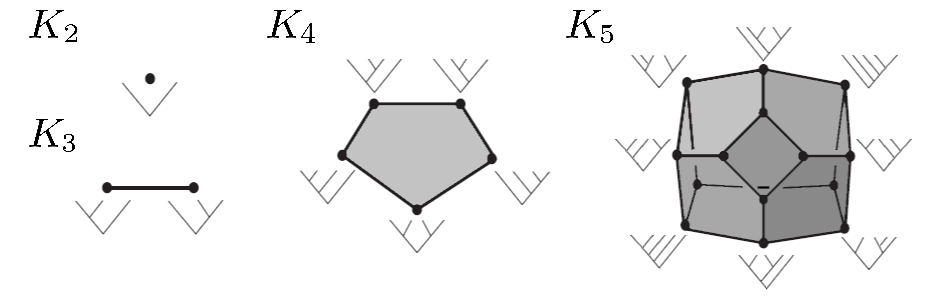
\includegraphics[width=0.72\linewidth]{fig01.png}
  \caption{前四个结合面体 $K_2,K_3,K_4,K_5$。顶点处的每一种拼接都可用一棵二叉树表示：
    例如 $K_2$ 只含一个点 $(f_1*f_2)\in\Omega X$，其二叉树平凡；$K_3$ 有两个顶点，分别对应
    $((f_1*f_2)*f_3)$ 与 $(f_1*(f_2*f_3))$；构成 $K_4$ 的各种拼接已在正文列出。另一方面，
    更高维的胞腔参数化分叉更多的树：例如 $K_3$ 的 1-胞腔由一棵三叉树标记，编码
    $f_1*f_2*f_3$。[来源：\texttt{http://pseudomonad.blogspot.com/2010/08/m-theory-lesson-345.html}]
    \hfill（原书 p.5）}
  \label{fig:01}
\end{figure}

这些 $K_n$ 称为\textbf{结合面体}（associahedra），由 Stasheff 在 \cite{Sta63} 中首次构造。
他把它们纳入 $A_\infty$-空间的定义：$A_\infty$-空间是带有相容映射族
$m_n:K_n\times Y^n\to Y$（$n\ge 2$）的拓扑空间 $Y$。如上所见，环路空间 $\Omega X$ 正是
$A_\infty$-空间的原型。此外，对任何这样的 $Y$，奇异上链复形 $C^\bullet(Y)$ 给出我们所遇到的
第一个 $A_\infty$-代数。下面说明其缘由。

\subsection{$A_\infty$-代数与态射}\label{sec:1.2}

全文中我们总在一个固定的基域 $\mathbb K$ 上工作，并假定分次取在 $\mathbb Z$ 上，除非另有
说明。我们先回顾分次向量空间与复形的基本内容（参看 \cite{Kel06} 第 2.1 节）。

\begin{Def}\label{def:1.1}
设 $V$ 为 $\mathbb Z$-分次 $\mathbb K$-向量空间，即形如 $V=\bigoplus_{p\in\mathbb Z}V^p$。
对 $n\in\mathbb Z$，其 \textbf{$n$ 次平移} $V[n]$ 是把所有指标向下移动 $n$ 次所得的分次向量空间，
即 $(V[n])^p=V^{p+n}$ 对一切 $p\in\mathbb Z$ 成立。记 $SV:=V[1]$，称之为 $V$ 的
\textbf{悬挂}（suspension）。

给定另一个分次向量空间 $V'$，分次向量空间之间的态射 $f:V\to V'[d]$ 是次数为
$d=|f|\in\mathbb Z$ 的齐次分次 $\mathbb K$-线性映射（于是次数为 $p=|v|$ 的齐次元素
$v\in V$ 被映为次数为 $p+d$ 的齐次元素 $f(v)\in V'$；为方便起见，我们常常省略态射的次数信息）。

分次向量空间及其态射构成范畴 $\mathsf{GradVect}$。
\end{Def}

考虑分次向量空间态射 $f:V\to V'$ 与 $g:W\to W'$ 的张量积
$f\otimes g:V\otimes W\to V'\otimes W'$ 时，结果服从 \textbf{Koszul 符号法则}：
\[
  (f\otimes g)(v\otimes w)=(-1)^{|g||v|}f(v)\otimes g(w),
\]
对一切齐次元素 $v\in V$，$w\in W$ 成立。

\begin{Def}\label{def:1.2}
若分次向量空间 $V$ 带有一个微分 $d_V:V\to V[1]$，即一个满足 $d_V\circ d_V=0$ 的 1 次齐次
态射，则称之为一个\textbf{（上链）复形}。我们定义 $d_{SV}:=-d_V$，并对分次向量空间态射
$f:V\to V'$ 定义
\[
  d(f):=d_{V'}\circ f-(-1)^{|f|}f\circ d_V .
\]
后者成为复形态射（上链映射）当且仅当 $d(f)=0$。

复形及其态射构成范畴 $\mathsf{Ch}$。因此我们可以研究它的上同调对应物 $H(\mathsf{Ch})$：
其对象是分次向量空间 $H(V)=\bigoplus_{p\in\mathbb Z}H^p(V)$，态射是诱导出的分次态射
（确实，作为范畴有 $H(\mathsf{Ch})\simeq\mathsf{GradVect}$）。
\end{Def}

最后回顾：复形态射 $f$ 与 $f'$ 同伦，当且仅当存在分次向量空间态射 $h$ 使得
$f-f'=d(h)$。同调代数学告诉我们，此时两者在上同调中诱导的映射相同：
$H^p(f)=H^p(f')$ 对一切 $p\in\mathbb Z$ 成立。

下面我们定义 $A_\infty$-代数，它也称为\textbf{强同伦结合代数}（strongly homotopy
associative algebra），其缘由将在下面的注 \ref{rem:1.5} 中明了。主要参考文献是
\cite{Kel01} 第 3–4 节。

\begin{Def}\label{def:1.3}
域 $\mathbb K$ 上的 \textbf{$A_\infty$-代数}是一个 $\mathbb Z$-分次 $\mathbb K$-向量空间
$A=\bigoplus_{p\in\mathbb Z}A^p$，带有分次态射 $m_n:A^{\otimes n}\to A[2-n]$（$n\ge 1$），
使得对一切 $n\ge 1$，作为 $A^{\otimes n}\to A$ 的映射成立方程
\begin{equation}\label{eq:1.1}
  \sum_{r+s+t=n}(-1)^{r+st}m_{r+1+t}
  \bigl(\mathrm{id}_A^{\otimes r}\otimes m_s\otimes\mathrm{id}_A^{\otimes t}\bigr)=0 .
\end{equation}
若 $A$ 带有某个 $1_A\in A^0$，使得 $m_1(1_A)=0$，
$m_2(1_A,a)=a=m_2(a,1_A)$ 对一切 $a\in A$ 成立，且当 $i>2$ 时
$m_i(\dots,1_A,\dots)=0$，则称 $A$ \textbf{严格幺的}（strictly unital）。
（若 $1_A$ 存在则唯一；称之为\textbf{严格单位元}。）

$A$ 的 \textbf{$A_\infty$-子代数} $B$ 是一个分次子空间，使得所有态射 $m_n$ 都限制到 $B$ 上。
\end{Def}

% [Tutor Note: 【易错】式 \eqref{eq:1.1} 的符号指数是 $r+st$，不是 $r+s+t$ 或 $rs+t$。它来自
% 把 $m_s$ 搬过前 $r$ 个因子的 Koszul 符号：$(-1)^{s\cdot 1\cdot r}$（每个 $m_s$ 的次数为
% $2-s$，故实际指数为 $r(2-s)+st$ 的化简结果，见 Keller 书中的推导）。逐项核对时务必先固定
% $r,s,t$ 再数 $m_s$ 与 $m_{r+1+t}$ 的相对位置。]

这里我们不必过分纠结式 \eqref{eq:1.1} 中出现的符号：具体的输入会按定义 \ref{def:1.1} 的
Koszul 法则对它作相应修改。在讨论 $A_\infty$-范畴时我们会更精确，那里所有公式都以这种形式
给出。

\begin{Rem}\label{rem:1.4}
若希望让定义 \ref{def:1.3} 中每个态射 $m_n$ 的次数与 $n$ 无关，有一种借助悬挂的典范做法：
通过要求下图交换，在诸 $m_n$ 与分次映射 $b_n:(SA)^{\otimes n}\to SA$ 之间建立一一对应：
\[
  \begin{tikzcd}
    A^{\otimes n} \arrow[r,"m_n"] \arrow[d,"s^{\otimes n}"'] & A \arrow[d,"s"] \\
    (SA)^{\otimes n} \arrow[r,"b_n"'] & SA
  \end{tikzcd}
\]
对一切 $n\ge 1$ 成立。这里 $s:A\to SA$，$a\in A^p\mapsto a\in(SA)^{p-1}$，次数为 $-1$，
于是每个 $b_n$ 满足 $|b_n|=-(-1)\cdot n+(2-n)+(-1)=1$。特别地，$b_1=-m_1$，且
$b_2(a_1,a_2)=(-1)^{|a_1|}m_2(a_1,a_2)$。可以证明：诸 $m_n$ 在 $A$ 上给出 $A_\infty$-代数
结构，当且仅当对一切 $n\ge 1$，
\[
  \sum_{r+s+t=n}b_{r+1+t}
  \bigl(\mathrm{id}_A^{\otimes r}\otimes b_s\otimes\mathrm{id}_A^{\otimes t}\bigr)=0 ,
\]
其中可以注意到，式 \eqref{eq:1.1} 中的符号已经消失。

具体操作中我们几乎从不真正使用悬挂，但在拼合各种符号约定时必须把它们考虑在内。
\end{Rem}

% [Tutor Note: 【含糊】注 \ref{rem:1.4} 中 "可以证明"（原文 one can prove）省略了证明：它等价于
% 同调微扰引理（HPT）在一维情形下的表述——把 $m_n$ 用 $s^{\otimes n}$ 共轭并消去 $\pm1$ 因子，
% 或用 $b_n=s\circ m_n\circ(s^{\otimes n})^{-1}$ 直接验证方程逐项相消。$|b_n|$ 的计算中
% "$-(-1)\cdot n$" 一项是 $(s^{\otimes n})^{-1}$ 的次数 $+n$（因为 $|s|=-1$），作者写成
% $(-1)\cdot n$ 再取负，易误读数。参见 Keller \cite{Kel01} 第 3 节。]

\begin{Rem}\label{rem:1.5}
方程组 \eqref{eq:1.1} 给出以下推论：
\begin{itemize}[leftmargin=2em]
  \item $m_1m_1=0$，于是 $(A,m_1)$ 是上链复形（从而按定义 $(SA,-m_1)$ 也是）。
  \item $m_1m_2=m_2(m_1\otimes\mathrm{id}_A+\mathrm{id}_A\otimes m_1)$ 表明微分 $m_1$ 是乘法%
  \footnote{我们称之为"乘法"，是因为在 $p\neq 0$ 时 $A^p=0$ 的特殊情形下，$A=A^0$ 只有
  $m_2$ 这一个非零映射，其次数为 $0$，因而可看作普通结合代数 $A$ 的乘法。}
  $m_2$ 的导子（即按分次 Leibniz 法则相容——正如所预期的那样）。由于
  $(m_1\otimes\mathrm{id}_A+\mathrm{id}_A\otimes m_1)$ 是 $A^{\otimes 2}$ 的微分，$m_2$ 是
  复形态射。
  \item $m_2(\mathrm{id}_A\otimes m_2-m_2\otimes\mathrm{id}_A)
  =m_1m_3+m_3(m_1\otimes\mathrm{id}_A\otimes\mathrm{id}_A+\mathrm{id}_A\otimes m_1\otimes
  \mathrm{id}_A+\mathrm{id}_A\otimes\mathrm{id}_A\otimes m_1)=d(m_3)$ 告诉我们：$m_2$ 只在
  同伦意义下结合！（"强同伦结合"这一术语即由此而来。）因此相应的上同调 $H(A)$ 关于
  $H(m_2)$ 构成分次结合代数（若 $H(A)$ 有单位元，则它由 $A$ 的上同调单位元诱导）。
  \item 若对一切 $n>2$ 有 $m_n=0$，则 $(A,m_1,m_2)$ 成为结合微分分次代数；反之，任何这样
  的代数都可看作 $A_\infty$-代数的特例。
\end{itemize}
\end{Rem}

第二个要点揭示了 $A_\infty$-代数的本性：它是结合性只在上同调意义下成立（且可能没有单位元）
的代数。第三个要点则已预示了在上同调层面工作的优势，这是我们后续理论的一条指导原则。

\begin{Def}\label{def:1.6}
给定两个 $A_\infty$-代数 $A$ 与 $B$，其态射分别为 $m_n^A$ 与 $m_n^B$，则
\textbf{$A_\infty$-代数态射} $f:A\to B$ 是一族分次映射 $f_n:A^{\otimes n}\to B[1-n]$
（$n\ge 1$），满足方程
\begin{equation}\label{eq:1.2}
  \sum_{r+s+t=n}(-1)^{r+st}f_{r+1+t}
  \bigl(\mathrm{id}_A^{\otimes r}\otimes m_s^A\otimes\mathrm{id}_A^{\otimes t}\bigr)
  =\sum_{\substack{1\le r\le n\\ s_1+\cdots+s_r=n}}(-1)^u\,
  m_r^B(f_{s_1}\otimes\cdots\otimes f_{s_r})
\end{equation}
对一切 $n\ge 1$ 成立，其中 $u:=\sum_{i=1}^{r-1}(r-i)(s_i-1)$。

与第二个 $A_\infty$-代数态射 $g:B\to C$ 的复合由下列分次映射族给出：
\[
  (g\circ f)_n:=\sum_{\substack{1\le r\le n\\ s_1+\cdots+s_r=n}}(-1)^u\,
  g_r\circ(f_{s_1}\otimes\cdots\otimes f_{s_r})
\]
（把它们代入式 \eqref{eq:1.2} 即可看出 $g\circ f:A\to C$ 确实是 $A_\infty$-代数态射）。

当 $A=B$ 时容易看出：取 $f_1:=\mathrm{id}_A$ 而其余 $f_n:=0$ 的 $f$ 对应于 $A$ 上的恒等态射。
\end{Def}

% [Tutor Note: 【易错】式 \eqref{eq:1.2} 右端的符号指数 $u=\sum_{i=1}^{r-1}(r-i)(s_i-1)$
% 极易抄错：每一项是 $(r-i)(s_i-1)$，不是 $(r-i)(s_i)$，也不含 $f$ 自身的次数。它来自把
% $m_r^B$ 依次搬过 $f_{s_1},\dots,f_{s_i}$ 时累积的 Koszul 符号。验证 $n=2$ 的项
% $f_1m_2^A-m_2^B(f_1\otimes f_1)=d(f_2)$ 是符号是否抄对的试金石。]

特别地，式 \eqref{eq:1.2} 的前两个等式
$f_1m_1^A=m_1^Bf_1$ 与
$f_1m_2^A-m_2^B(f_1\otimes f_1)
=m_1^Bf_2+f_2(m_1^A\otimes\mathrm{id}_A+\mathrm{id}_A\otimes m_1^A)=d(f_2)$
告诉我们：$f_1$ 是复形态射，且只在与 $m_2$ 同伦的意义下与 $m_2$ 交换。同样，使用悬挂后
式 \eqref{eq:1.2} 中的符号即可省去（见注 \ref{rem:1.4}）。

最后我们给出几个稍后会在其 $A_\infty$-范畴形式中重现的定义。

\begin{Def}\label{def:1.7}
若 $A_\infty$-代数态射 $f:A\to B$ 的 $f_1$ 是拟同构，即它诱导出代数同构
$H(f_1):H(A)\to H(B)$，则称 $f$ 为\textbf{拟同构}。

严格幺 $A_\infty$-代数之间的态射 $f:(A,1_A)\to(B,1_B)$，若满足 $f_1(1_A)=1_B$ 且
$f_i(\dots,1_A,\dots)=0$（$i>1$），则称 $f$ 本身是\textbf{严格幺的}。
\end{Def}

\subsection{$A_\infty$-模与态射}\label{sec:1.3}

\begin{Def}\label{def:1.8}
设 $A$ 为 $A_\infty$-代数，其态射 $m_n^A$ 如定义 \ref{def:1.3} 所述。$A$ 上的
\textbf{$A_\infty$-模}是一个 $\mathbb Z$-分次 $\mathbb K$-向量空间
$M=\bigoplus_{p\in\mathbb Z}M^p$，带有映射 $m_n^M:M\otimes A^{\otimes n-1}\to M[2-n]$
（$n\ge 1$），它们满足与式 \eqref{eq:1.1} 类似的方程
\begin{equation}\label{eq:1.3}
  \begin{aligned}
    \sum_{r+s+t=n}(-1)^{r+st}m_{r+1+t}^M
    \bigl(\mathrm{id}_M\otimes\mathrm{id}_A^{\otimes r-1}\otimes m_s^A
    \otimes\mathrm{id}_A^{\otimes t}\bigr)&=0
    &&\text{若 } r>0,\\
    \sum_{s+t=n}(-1)^{st}m_{1+t}^M\bigl(m_s^M\otimes\mathrm{id}_A^{\otimes t}\bigr)&=0
    &&\text{若 } r=0.
  \end{aligned}
\end{equation}
\end{Def}

\begin{Def}\label{def:1.9}
设 $M$ 与 $N$ 为 $A_\infty$-代数 $A$ 上的 $A_\infty$-模，其态射分别为 $m_n^M$ 与 $m_n^N$。
\textbf{$A_\infty$-模态射} $f:M\to N$ 是一族分次映射
$f_n:M\otimes A^{\otimes n-1}\to N[1-n]$（$n\ge 1$），满足方程
\begin{equation}\label{eq:1.4}
  \sum_{r+s+t=n}(-1)^{r+st}f_{r+1+t}
  \bigl(\mathrm{id}_A^{\otimes r}\otimes m_s^M\otimes\mathrm{id}_A^{\otimes t}\bigr)
  =\sum_{s+t=n}(-1)^{(s+1)t}m_{1+t}^N\bigl(f_s\otimes\mathrm{id}_A^{\otimes t}\bigr)
\end{equation}
对一切 $n\ge 1$ 成立；其中必须像上一个定义那样区分 $r>0$ 与 $r=0$ 两种情形。

与第二个 $A_\infty$-模态射 $g:N\to P$ 的复合由下列分次映射族给出：
\[
  (g\circ f)_n:=\sum_{s+t=n}(-1)^{(s-1)t}f_{1+t}\circ\bigl(g_s\otimes
  \mathrm{id}_A^{\otimes t}\bigr)
\]
（可以证明它们满足方程 \eqref{eq:1.4}）。恒等态射与拟同构的定义与 $A_\infty$-代数情形相同。

$A_\infty$-模连同 $A_\infty$-模态射构成一个范畴，记作 $\mathcal C_\infty(\mathcal A)$。
\end{Def}

% [Tutor Note: 【易错】定义 \ref{def:1.9} 中 $r=0$ 的分支在式 \eqref{eq:1.4} 右端出现，
% 但左端求和仍写作 $r+s+t=n$；实际约定是：$r=0$ 时左端只剩 $s+t=n$ 的项且
% $m_s^M$ 直接作用在 $M$ 上。书写代码时若把两个分支合并，最常见错误是漏掉 $r=0$ 时
% $m_s^M$ 前少一个 $\mathrm{id}_A^{\otimes r}$ 因子。

现在我们已经初步领略了第一部分所处理的代数结构，接下来转向更一般的 $A_\infty$-范畴概念。

% ============================================================================
% 第 2 章  $A_\infty$-范畴  （原书 pp.10–27，PDF pp.13–30）
% 底本：Alessandro Imparato, Towards Homological Mirror Symmetry, ETH Zürich
% 说明：章标题中的 ∞ 以 $A_\infty$ 排出，避免中文字库缺字。
% 公式编号：原文全书连续编号，本章为 (5)–(33)；main.tex 已改为全书连续编号，
%           故每个带号 equation 环境自动得到与原文一致的编号，不得手工 \tag。
%           本章共 29 个编号公式，恰与原文一一对应；多行公式一律 equation+aligned。
% ============================================================================
\section{$A_\infty$-范畴}\label{ch:02}

\takeaway{%
  核心图像：$A_\infty$-范畴是“同伦意义下的范畴”：复合 $\mu^2$ 只在上同调层面结合，
  高阶运算 $\mu^d$ 精确记录结合律失效的程度。\\
  数学工具：分次线性范畴与上链复形、$A_\infty$-结合性方程、结合面体 $K_n$ 的组合学、
  Hochschild 上同调、同调微扰引理。\\
  主要结论：$\mu^1$ 使每个 Hom 集成为复形，$H(\mathcal A)$ 是通常范畴；预自然变换构成
  函子范畴；拟等价在 $H^0$ 中可逆；Yoneda 嵌入全忠实地映入 $A_\infty$-模范畴。%
}

\subsection{范畴论预备}\label{sec:2.1}

在着手研究 $A_\infty$-范畴之前，我们先把范畴论中若干基本定义与结论汇总于此：
它们在本书中频繁出现，并在后文的证明里起关键作用。回忆：我们始终在某个固定的基域
$\mathbb K$ 上工作。

\begin{Def}\label{def:2.1}
称范畴 $\mathsf C$ 为：
\begin{itemize}
  \item \emph{线性的}（linear）且\emph{分次的}（graded），若其所有 Hom 集都是分次
        $\mathbb K$-向量空间，并且相容态射的复合是 $\mathbb K$ 上的双线性运算；
  \item \emph{微分 $\mathbb Z$-分次的}（dg），若每个 Hom 集都是 $\mathbb Z$-分次的
        （上链）复形，从而态射的复合是上链映射，且每个恒等态射的微分等于零
        （例：定义 \ref{def:1.2} 中的范畴 $\mathsf{Ch}$）；
  \item \emph{小的}（small），若 $\operatorname{obj}(\mathsf C)$ 与所有 Hom 集的全体
        都是集合；
  \item \emph{非幺的}（non-unital），若它可能缺少某些恒等态射（此时 $\mathsf C$ 并非
        真正的范畴）。
\end{itemize}
\end{Def}
% [Tutor Note: 【易错】“线性且分次”一条只要求齐次相容态射之间的复合双线性；非齐次情形由线性延拓定义，原文用 compatible 一词正是指“齐次且次数相加”的态射对。]
% [Tutor Note: 【背景】dg 范畴中“恒等态射的微分为零”并非额外公理：在 $\mathsf{Ch}$ 里 $d(f)=d_W\circ f-(-1)^{|f|}f\circ d_V$，故 $d(\mathrm{id}_V)=0$ 自动成立；参看定义 \ref{def:1.2} 的约定。]

\begin{Def}\label{def:2.2}
设 $\mathsf C$ 与 $\mathsf D$ 为范畴。函子 $F:\mathsf C\to\mathsf D$ 称为：
\begin{itemize}
  \item \emph{同构}，若存在函子 $G:\mathsf D\to\mathsf C$，使得作为函子有
        $G\circ F=\mathrm{Id}_{\mathsf C}$ 且 $F\circ G=\mathrm{Id}_{\mathsf D}$；
        此时称 $\mathsf C$ 与 $\mathsf D$ \emph{同构}；
  \item \emph{等价}，若存在函子 $G:\mathsf D\to\mathsf C$（有时称为\emph{拟逆}）以及
        自然同构 $\Phi:\mathrm{Id}_{\mathsf C}\to G\circ F$、$\Psi:F\circ G\to
        \mathrm{Id}_{\mathsf D}$（意即：对 $X\in\operatorname{obj}(\mathsf C)$，每个
        $\Phi_X\in\Hom_{\mathsf C}\bigl(X,G(F(X))\bigr)$ 都是对象的同构；对
        $Y\in\operatorname{obj}(\mathsf D)$，每个 $\Psi_Y\in
        \Hom_{\mathsf D}(F(G(Y)),Y)$ 亦然）；此时称 $\mathsf C$ 与 $\mathsf D$
        \emph{等价}；
  \item \emph{全的}与\emph{忠实的}，若对一切 $X,Y\in\operatorname{obj}(\mathsf C)$，
        映射 $F_{X,Y}:\Hom_{\mathsf C}(X,Y)\to\Hom_{\mathsf D}(F(X),F(Y))$ 分别是满射、
        单射（两者兼有时称为\emph{全忠实}）；
  \item \emph{本质满的}，若对每个 $Y\in\operatorname{obj}(\mathsf D)$，都存在
        $X\in\operatorname{obj}(\mathsf C)$ 以及对象的同构
        $f\in\Hom_{\mathsf D}(Y,F(X))$；
  \item \emph{嵌入}，若它忠实且在对象上单射（即 $F(X_1)=F(X_2)\in
        \operatorname{obj}(\mathsf D)$ 蕴含 $X_1=X_2\in\operatorname{obj}(\mathsf C)$）；
  \item \emph{线性的}与\emph{分次的}，若上述每个 $F_{X,Y}$ 都是分次向量空间之间的
        $\mathbb K$-线性分次态射（设 $\mathsf C,\mathsf D$ 线性且分次）；
  \item （\emph{非}）\emph{幺的}，若它（不）把一切恒等态射送到恒等态射。
\end{itemize}
\end{Def}

下列结论都是上述定义的简单推论（例如其证明可在 \cite{GM03} 中找到）。

\begin{Lem}\label{lem:2.3}
函子 $F:\mathsf C\to\mathsf D$：
\begin{enumerate}
  \item 是同构，当且仅当它在对象上与 Hom 集上都是双射；
  \item 是等价，当且仅当它全、忠实且本质满。
\end{enumerate}
特别地，同构都是等价，从而是全忠实的。
\end{Lem}

% [Tutor Note: 【易错】引理 \ref{lem:2.3} 第 2 条中“全、忠实、本质满”三者缺一不可：仅“全且忠实”只给出与某个满子范畴的等价，本质满才补上对象的覆盖。]

此后若无另行说明，我们总假定所讨论的（$A_\infty$-）范畴都是线性的且小的。

\subsection{$A_\infty$-范畴与 $A_\infty$-函子}\label{sec:2.2}

\begin{Def}\label{def:2.4}
一个非幺 $A_\infty$-范畴 $\mathcal A$ 由以下数据组成：
\begin{itemize}
  \item 一个对象集 $\operatorname{obj}(\mathcal A)$；
  \item 对任意一对 $X_0,X_1\in\operatorname{obj}(\mathcal A)$，一个 $\mathbb Z$-分次的
        $\mathbb K$-向量空间
        \[
          \hom_{\mathcal A}(X_0,X_1)=\bigoplus_{p\in\mathbb Z}
          \hom^p_{\mathcal A}(X_0,X_1),
        \]
        其元素仍称为态射（属于 $\hom^p_{\mathcal A}(X_0,X_1)$ 时称为 $p$ 次齐次的）；
  \item （多）线性分次映射
        \begin{equation}\label{eq:2.5}
          \mu^d_{\mathcal A}:\hom_{\mathcal A}(X_{d-1},X_d)\otimes\dots\otimes
          \hom_{\mathcal A}(X_0,X_1)\longrightarrow\hom_{\mathcal A}(X_0,X_d)[2-d]
        \end{equation}
        对每个 $d\ge 1$ 与 $X_0,\dots,X_d\in\operatorname{obj}(\mathcal A)$ 给出，
        我们称之为\emph{复合映射}。它们必须满足二次的 \emph{$A_\infty$-结合性方程}
        \begin{equation}\label{eq:2.6}
          \sum_{\substack{1\le m\le d\\ 0\le n\le d-m}}
          (-1)^{\dagger_n}\mu^{d-m+1}_{\mathcal A}\bigl(a_d,\dots,a_{n+m+1},
          \underbrace{\mu^m_{\mathcal A}(a_{n+m},\dots,a_{n+1})}
          _{\in\hom_{\mathcal A}(X_n,X_{n+m})},a_n,\dots,a_1\bigr)=0
        \end{equation}
        在 $\hom_{\mathcal A}(X_0,X_d)$ 中成立，其中
        $a_i\in\hom_{\mathcal A}(X_{i-1},X_i)$，且
        $\dagger_n:=\bigl(\sum_{i=1}^n|a_i|\bigr)-n$。\footnote{$\dagger_n$ 连同其他
        调节我们各表达式符号的变量，此后都作为标准记号使用，不再另行说明。}
\end{itemize}
\end{Def}
% [Tutor Note: 【易错】\eqref{eq:2.5} 中最左的因子是 $\hom_{\mathcal A}(X_{d-1},X_d)$：$\mu^d$ 的第一个变量是“最靠右”的态射。这是 Seidel 采用的记号，与按 $X_0\to X_1\to\cdots$ 自左向右排列的某些文献（如 Keller）相反，套用公式前务必核对变量次序。]
% [Tutor Note: 【易错】$\dagger_n$ 减去的是 $n$ 而不是 $n(n+1)/2$：作者把每个 $a_i$ 的“平移次数”$|a_i|-1$ 求和，故 $\dagger_n=\sum_{i=1}^n(|a_i|-1)$。]

对 $d=1,2$，前两个这样的方程形如
\[
  \mu^1_{\mathcal A}\bigl(\mu^1_{\mathcal A}(a_1)\bigr)=0
  \quad\text{与}\quad
  \mu^1_{\mathcal A}\bigl(\mu^2_{\mathcal A}(a_2,a_1)\bigr)
  =(-1)^{|a_1|}\mu^2_{\mathcal A}\bigl(\mu^1_{\mathcal A}(a_2),a_1\bigr)
  -\mu^2_{\mathcal A}\bigl(a_2,\mu^1_{\mathcal A}(a_1)\bigr).
\]

$A_\infty$-子范畴 $\mathcal B\subset\mathcal A$ 是指这样的 $A_\infty$-范畴：
$\operatorname{obj}(\mathcal B)\subset\operatorname{obj}(\mathcal A)$，对一切
$X_0,X_1\in\operatorname{obj}(\mathcal B)$ 都有 $\hom_{\mathcal B}(X_0,X_1)\subset
\hom_{\mathcal A}(X_0,X_1)$ 为分次子空间，且复合映射 $\mu^d_{\mathcal B}$ 的靶空间
落在 $\mathcal B$ 之内。

式 \eqref{eq:2.5} 与 \eqref{eq:2.6} 的指标体例可能略有误导：它试图调和若干标准约定。
为保持一致，此处及此后我们都忠实采用 Seidel 在 \cite{Sei08} 中所用的记号。

\begin{Rem}\label{rem:2.5}
考虑 $\operatorname{obj}(\mathcal A):=\{X\}$ 的情形。此时唯一可能的 $\mathbb Z$-分次
向量空间 $\mathcal A:=\hom_{\mathcal A}(X,X)$ 配上分次映射 $m_n:=\mu^n_{\mathcal A}$
确实构成 $A_\infty$-代数，因为方程 \eqref{eq:1.1} 与 \eqref{eq:2.6} 恰好重合（可能相差一个符号）。

此外，若 $d>2$ 时 $\mu^d_{\mathcal A}=0$，则 $A_\infty$-范畴 $\mathcal A$ 就是微分分次
范畴，反之亦然（例如 dg 范畴 $\mathsf{Ch}$ 可视为 $A_\infty$-范畴）。
\end{Rem}
% [Tutor Note: 【易错】注 \ref{rem:2.5} 说方程 \eqref{eq:1.1} 与 \eqref{eq:2.6} “可能相差一个符号”：若第 1 章采用 $(-1)^{|a_2|}$ 或 $(-1)^{|a_1|}$ 的不同 Koszul 约定，两者就不止差一个整体符号，而是逐项符号的重新分配；引用时须回到第 1 章定义 \ref{def:1.1} 核对。]

$A_\infty$-结合性方程给出与注 \ref{rem:1.5} 中对 $A_\infty$-代数完全相同的结论：非幺
$A_\infty$-范畴一般不是范畴，因为它们可能缺少恒等态射，而且每个复合映射
$\mu^2_{\mathcal A}$ 未必结合。

然而 $\mu^1_{\mathcal A}\mu^1_{\mathcal A}=0$，所以每个态射空间
$\hom_{\mathcal A}(X_0,X_1)$ 都是上链复形，其微分为
$\mu^1_{\mathcal A}:\hom_{\mathcal A}(X_0,X_1)\to\hom_{\mathcal A}(X_0,X_1)[1]$。
于是谈论\emph{上闭链}（即满足 $\mu^1_{\mathcal A}(a)=0$ 的任意
$a\in\hom_{\mathcal A}(X_0,X_1)$）、\emph{上边缘}（即对某个
$b\in\hom_{\mathcal A}(X_0,X_1)$ 形如 $a=\mu^1_{\mathcal A}(b)$ 的任意 $a$）与
\emph{上同调}才有意义：

\begin{Def}\label{def:2.6}
设 $\mathcal A$ 为非幺 $A_\infty$-范畴。它的\emph{上同调范畴} $H(\mathcal A)$
定义如下：$\operatorname{obj}(H(\mathcal A)):=\operatorname{obj}(\mathcal A)$，
每对 $X_0,X_1\in\operatorname{obj}(\mathcal A)$ 给出一个分次上同调群
\begin{equation}\label{eq:2.7}
  \Hom_{H(\mathcal A)}(X_0,X_1):=H\bigl(\hom_{\mathcal A}(X_0,X_1)\bigr)
  =\bigoplus_{p\in\mathbb Z}H^p\bigl(\hom_{\mathcal A}(X_0,X_1)\bigr),
\end{equation}
而“通常的”结合（！）复合映射为\footnote{注意记号的选择：凡谈及上同调范畴，
我们都在“Hom”中使用大写“H”（相对于 $A_\infty$-范畴的“hom”），并采用复合符号
“$\circ$”。}
\begin{equation}\label{eq:2.8}
  \begin{gathered}
    \circ:\Hom_{H(\mathcal A)}(X_1,X_2)\times\Hom_{H(\mathcal A)}(X_0,X_1)
    \longrightarrow\Hom_{H(\mathcal A)}(X_0,X_2),\\
    (\langle a_2\rangle,\langle a_1\rangle)\longmapsto
    \langle a_2\rangle\circ\langle a_1\rangle
    :=(-1)^{|a_1|}\langle\mu^2_{\mathcal A}(a_2,a_1)\rangle.
  \end{gathered}
\end{equation}
这是一个非幺的通常线性分次范畴。
\end{Def}
% [Tutor Note: 【易错】\eqref{eq:2.8} 中的符号 $(-1)^{|a_1|}$ 容易漏：$\mu^2$ 本身并不是 $H(\mathcal A)$ 的复合，差一个 Koszul 符号；也正因如此，$\circ$ 才结合（由 \eqref{eq:2.6} 在 $d=3$ 时的项保证）。]

我们记 $H^0(\mathcal A)\subset H(\mathcal A)$ 为\emph{零阶上同调子范畴}，其
$\operatorname{obj}(H^0(\mathcal A)):=\operatorname{obj}(H(\mathcal A))$，
$\Hom_{H^0(\mathcal A)}(X_0,X_1):=H^0\bigl(\hom_{\mathcal A}(X_0,X_1)\bigr)$。

\begin{Def}\label{def:2.7}
两个非幺 $A_\infty$-范畴 $\mathcal A$ 与 $\mathcal B$ 之间的\emph{非幺
$A_\infty$-函子} $\mathcal F:\mathcal A\to\mathcal B$ 是一个映射
$\mathcal F:\operatorname{obj}(\mathcal A)\to\operatorname{obj}(\mathcal B)$，
连同对每个 $d\ge 1$ 与 $X_0,\dots,X_d\in\operatorname{obj}(\mathcal A)$ 给出的一列
（多）线性分次映射
\begin{equation}\label{eq:2.9}
  \mathcal F^d:\hom_{\mathcal A}(X_{d-1},X_d)\otimes\dots\otimes
  \hom_{\mathcal A}(X_0,X_1)\longrightarrow
  \hom_{\mathcal B}\bigl(\mathcal F(X_0),\mathcal F(X_d)\bigr)[1-d],
\end{equation}
它们满足方程
\begin{equation}\label{eq:2.10}
  \begin{aligned}
    &\sum_{\substack{1\le r\le d\\ s_1+\dots+s_r=d}}
    \mu^r_{\mathcal B}\bigl(\mathcal F^{s_r}(a_d,\dots,a_{d-s_r+1}),\dots,
    \mathcal F^{s_1}(a_{s_1},\dots,a_1)\bigr)\\
    &\qquad=\sum_{\substack{1\le m\le d\\ 0\le n\le d-m}}(-1)^{\dagger_n}
    \mathcal F^{d-m+1}\bigl(a_d,\dots,a_{n+m+1},
    \mu^m_{\mathcal A}(a_{n+m},\dots,a_{n+1}),a_n,\dots,a_1\bigr),
  \end{aligned}
\end{equation}
在 $\hom_{\mathcal B}\bigl(\mathcal F(X_0),\mathcal F(X_d)\bigr)$ 中成立，其中
$a_i\in\hom_{\mathcal A}(X_{i-1},X_i)$。
\end{Def}

给定另一个非幺 $A_\infty$-函子 $\mathcal G:\mathcal B\to\mathcal C$，复合
$\mathcal G\circ\mathcal F:\mathcal A\to\mathcal C$ 是严格结合的，它由下式指定为
$A_\infty$-函子：
\begin{equation}\label{eq:2.11}
  (\mathcal G\circ\mathcal F)^d(a_d,\dots,a_1):=
  \sum_{\substack{1\le r\le d\\ s_1+\dots+s_r=d}}
  \mathcal G^r\bigl(\mathcal F^{s_r}(a_d,\dots,a_{d-s_r+1}),\dots,
  \mathcal F^{s_1}(a_{s_1},\dots,a_1)\bigr)
\end{equation}
取值于 $\hom_{\mathcal C}\bigl(\mathcal G(\mathcal F(X_0)),\mathcal G(\mathcal
F(X_d))\bigr)$ 中（可以证明它们确实满足定义方程 \eqref{eq:2.10}）。特别地，
$(\mathcal G\circ\mathcal F)^1(a_1)=\mathcal G^1(\mathcal F^1(a_1))$ 且
$(\mathcal G\circ\mathcal F)^2(a_2,a_1)=\mathcal G^1(\mathcal F^2(a_2,a_1))
+\mathcal G^2(\mathcal F^1(a_2),\mathcal F^1(a_1))$。

若 $\mathcal A=\mathcal B$ 且 $\mathcal A$ 幺，则恒等 $A_\infty$-函子
$\mathrm{Id}_{\mathcal A}$ 由 $\mathrm{Id}_{\mathcal A}(X):=X$、$X\in
\operatorname{obj}(\mathcal A)$ 时 $\mathrm{Id}^1_{\mathcal A}:=
\mathrm{id}_{\hom_{\mathcal A}(X,X)}$ 以及一切 $k>1$ 时
$\mathrm{Id}^k_{\mathcal A}:=0$ 给出。

正如所料，单对象 $A_\infty$-范畴之间的 $A_\infty$-函子恰是 $A_\infty$-代数态射。

由式 \eqref{eq:2.10} 可以推出各自的一阶映射交换：对任意
$a_1\in\hom_{\mathcal A}(X_0,X_1)$ 有
$\mu^1_{\mathcal B}\bigl(\mathcal F^1(a_1)\bigr)=
\mathcal F^1\bigl(\mu^1_{\mathcal A}(a_1)\bigr)$。$d=2$ 的情形则给出
\[
  \mu^1_{\mathcal B}\bigl(\mathcal F^2(a_2,a_1)\bigr)
  +\mu^2_{\mathcal B}\bigl(\mathcal F^1(a_2),\mathcal F^1(a_1)\bigr)
  =\mathcal F^1\bigl(\mu^2_{\mathcal A}(a_2,a_1)\bigr)
  +\mathcal F^2\bigl(a_2,\mu^1_{\mathcal A}(a_1)\bigr)
  +(-1)^{|a_1|-1}\mathcal F^2\bigl(\mu^1_{\mathcal A}(a_2),a_1\bigr).
\]
这些方程与我们从定义 \ref{def:1.6} 得到的结果相容（同样相差某些符号）。
% [Tutor Note: 【勘误】原书 p.12 此式写作 $\mathcal F^2(a_2,A^1(a_1))$，其中 $A^1$ 显然是 $\mu^1_{\mathcal A}$ 的笔误（与同式其余各项对照即可判定）；译文按 $\mu^1_{\mathcal A}$ 排出，原文照录于此备考。]

\begin{Def}\label{def:2.8}
非幺 $A_\infty$-函子 $\mathcal F:\mathcal A\to\mathcal B$ 诱导\emph{上同调函子}
$H(\mathcal F):H(\mathcal A)\to H(\mathcal B)$：它把 $X\in
\operatorname{obj}(H(\mathcal A))$ 映为 $\mathcal F(X)\in
\operatorname{obj}(H(\mathcal B))$，并对每个 $X_0,X_1\in
\operatorname{obj}(H(\mathcal A))$ 把
\begin{equation}\label{eq:2.12}
  \langle a_1\rangle\in\Hom_{H(\mathcal A)}(X_0,X_1)
  \longmapsto\langle\mathcal F^1(a_1)\rangle\in
  \Hom_{H(\mathcal B)}\bigl(\mathcal F(X_0),\mathcal F(X_1)\bigr).
\end{equation}
这是通常的非幺线性分次函子。我们称 $\mathcal F$：
\begin{itemize}
  \item \emph{拟同构}，若 $H(\mathcal F)$ 是同构；
  \item \emph{上同调全忠实}，若 $H(\mathcal F)$ 全且忠实；
  \item \emph{上同调本质满}，若 $H(\mathcal F)$ 本质满。
\end{itemize}
注意 $H(\mathcal F):H(\mathcal A)\to H(\mathcal B)$ 本身在零阶上同调范畴上退化为
$H^0(\mathcal F):H^0(\mathcal A)\to H^0(\mathcal B)$。
\end{Def}

作为引理 \ref{lem:2.3} 的直接推论，拟同构都是上同调全忠实的 $A_\infty$-函子。

有一类特殊的 $A_\infty$-函子，它将在简化若干证明的框架时派上用场。该定义利用如下
（非平凡的）事实：给定 $A_\infty$-范畴 $\mathcal A$ 以及一列如式 \eqref{eq:2.9} 那样的
分次映射 $(\Phi^0,\Phi^1,\dots)$，若
$\Phi^1:\hom_{\mathcal A}(X_0,X_1)\to\hom_{\mathcal A}(X_0,X_1)$ 是线性自同构，
则关于 $\mu_{\mathcal B}$ 递归求解方程 \eqref{eq:2.10}，会给出 $\mathcal A$ 上唯一的
另一种 $A_\infty$-结构 $\tilde{\mathcal A}$，它由
$\operatorname{obj}(\tilde{\mathcal A}):=\operatorname{obj}(\mathcal A)$、
$\hom_{\tilde{\mathcal A}}(X_0,X_1):=\hom_{\mathcal A}(X_0,X_1)$ 与
$\mu_{\tilde{\mathcal A}}:=\mu_{\mathcal B}$ 给出。于是按构造，多线性分次映射
$\Phi^d$ 满足 \eqref{eq:2.10}。
% [Tutor Note: 【含糊】“递归求解……给出唯一结构”是原文明确标为 non-trivial 的一步，未给证明。其可行性依赖 $\Phi^1$ 可逆：逐阶解 $d=1,2,\dots$ 时，只有 $\Phi^1$ 出现的那一项可解出新的 $\mu^d$，其余项已由低阶确定；参见 \cite{Sei08} 第 (1e) 节或 \cite{Kel06} 第 2 节。]

\begin{Def}\label{def:2.9}
设 $\mathcal A$ 为 $A_\infty$-范畴，其另一种 $A_\infty$-结构
$\tilde{\mathcal A}$ 如上由一列分次映射 $(\Phi^0,\Phi^1,\dots)$ 构造。相应的非幺
$A_\infty$-函子 $\Phi:\mathcal A\to\Phi_*\mathcal A:=\tilde{\mathcal A}$ 称为
\emph{形式微分同胚}（formal diffeomorphism）。由式 \eqref{eq:2.12} 与 $\Phi^1$
的选取，它特别地是拟同构（从而是上同调全忠实的）。
\end{Def}
% [Tutor Note: 【易错】形式微分同胚的靶范畴 $\Phi_*\mathcal A$ 与 $\mathcal A$ 有相同的对象和态射空间，只换了高阶运算 $\mu^d$；它不是 $\mathcal A$ 的“子范畴”或“商范畴”，这一点在 §\ref{sec:2.7} 用 $\Phi$ 把 c-幺范畴换成严格幺范畴时至关重要。]

\subsection{预自然变换与复合}\label{sec:2.3}

在通常的范畴论中，我们可以考察函子之间的映射，即自然变换。对 $A_\infty$-函子当然也有
相应的推广。

\begin{Def}\label{def:2.10}
给定两个非幺 $A_\infty$-范畴 $\mathcal A$ 与 $\mathcal B$，定义
$\mathcal Q=\mathrm{nu\text{-}fun}(\mathcal A,\mathcal B)$ 为由以下数据指定的非幺
$A_\infty$-范畴：
\begin{itemize}
  \item 一个对象集 $\operatorname{obj}(\mathcal Q)$，由非幺 $A_\infty$-函子
        $\mathcal F:\mathcal A\to\mathcal B$ 组成；
  \item 对任意一对 $\mathcal F_0,\mathcal F_1\in\operatorname{obj}(\mathcal Q)$，
        态射的齐次部分 $T\in\hom^g_{\mathcal Q}(\mathcal F_0,\mathcal F_1)$ 是序列
        $(T^0,T^1,\dots)$，其中每个 $d\ge 1$ 的 $T^d$ 是一族（多）线性分次映射
        \begin{equation}\label{eq:2.13}
          \hom_{\mathcal A}(X_{d-1},X_d)\otimes\dots\otimes
          \hom_{\mathcal A}(X_0,X_1)\longrightarrow
          \hom_{\mathcal B}\bigl(\mathcal F_0(X_0),\mathcal F_1(X_d)\bigr)[g-d],
        \end{equation}
        其中 $X_0,\dots,X_d\in\operatorname{obj}(\mathcal A)$。而 $T^0$ 必须视为一族
        \[
          \bigl\{T^0_X\equiv T^0(X)\in\hom^g_{\mathcal B}\bigl(\mathcal F_0(X),
          \mathcal F_1(X)\bigr)\mid X\in\operatorname{obj}(\mathcal A)\bigr\}
        \]
        （与自然变换的标准定义一致）。称 $T$ 为从 $\mathcal F_0$ 到 $\mathcal F_1$ 的、
        次数为 $|T|=g$ 的\emph{预自然变换}；
  \item 复合映射 $\mu^d_{\mathcal Q}$ 形如 \eqref{eq:2.5} 中的那些，从而对
        $T_k\in\hom_{\mathcal Q}(\mathcal F_{k-1},\mathcal F_k)$，输出
        $S:=\mu^d_{\mathcal Q}(T_d,\dots,T_1)\in\hom_{\mathcal Q}(\mathcal F_0,
        \mathcal F_d)[2-d]$ 仍是形如 \eqref{eq:2.13} 的序列 $(S^0,S^1,\dots)$。
        前两种情形 $d=1,2$ 为\footnote{注意：按定义，在 \eqref{eq:2.14} 中只有 $s_i$
        可以为零，而在 \eqref{eq:2.15} 中 $s_i$ 与 $s_j$ 都可以为零。}
        \begin{equation}\label{eq:2.14}
          \begin{aligned}
            &\mu^1_{\mathcal Q}(T_1)^h(a_h,\dots,a_1)\\
            &\quad:=\sum_{\substack{1\le r\le h+1\\ 1\le i\le r\\ s_1+\dots+s_r=h}}
            (-1)^{\ddagger^1_i}\mu^r_{\mathcal B}\Bigl(
            \mathcal F_1^{s_r}(a_h,\dots,a_{h-s_r+1}),\dots,\\
            &\qquad\qquad \mathcal F_1^{s_{i+1}}(a_{h-\dots-s_{i+2}},\dots,
            a_{s_1+\dots+s_{i+1}}),T_1^{s_i}(a_{s_1+\dots+s_i},\dots,
            a_{s_1+\dots+s_{i-1}+1}),\\
            &\qquad\qquad \mathcal F_0^{s_{i-1}}(a_{s_1+\dots+s_{i-1}},\dots,
            a_{s_1+\dots+s_{i-2}+1}),\dots,\mathcal F_0^{s_1}(a_{s_1},\dots,a_1)
            \Bigr)\\
            &\qquad-\sum_{\substack{1\le m\le h\\ 0\le n\le h-m}}
            (-1)^{\dagger_n+|T_1|-1}T_1^{h-m+1}\bigl(a_h,\dots,
            \mu^m_{\mathcal A}(a_{n+m},\dots,a_{n+1}),\dots,a_1\bigr)
          \end{aligned}
        \end{equation}
        取值于 $\hom_{\mathcal B}(\mathcal F_0(X_0),\mathcal F_1(X_h))$ 中；而
        \begin{equation}\label{eq:2.15}
          \begin{aligned}
            &\mu^2_{\mathcal Q}(T_2,T_1)^h(a_h,\dots,a_1)\\
            &\quad:=\sum_{\substack{1\le r\le h+2\\ i<j\le r\\
            s_1+\dots+s_r=h}}(-1)^{\ddagger^1_i+\ddagger^2_j}
            \mu^r_{\mathcal B}\Bigl(\mathcal F_2^{s_r}(a_h,\dots,a_{h-s_r+1}),\dots,\\
            &\qquad\qquad \mathcal F_2^{s_{j+1}}(\dots),T_2^{s_j}(a_{s_1+\dots+s_j},
            \dots,a_{s_1+\dots+s_{j-1}+1}),\mathcal F_1^{s_{j-1}}(\dots),\dots,\\
            &\qquad\qquad \mathcal F_1^{s_{i+1}}(\dots),T_1^{s_i}(a_{s_1+\dots+s_i},
            \dots,a_{s_1+\dots+s_{i-1}+1}),\mathcal F_0^{s_{i-1}}(\dots),\dots,
            \mathcal F_0^{s_1}(a_{s_1},\dots,a_1)\Bigr)
          \end{aligned}
        \end{equation}
        取值于 $\hom_{\mathcal B}(\mathcal F_0(X_0),\mathcal F_2(X_h))$ 中，其中
        $h\ge 1$、$a_k\in\hom_{\mathcal A}(X_{k-1},X_k)$，且
        $\ddagger^j_i:=\bigl(|T_j|-1\bigr)\cdot\sum_{k=1}^{s_1+\dots+s_{i-1}}
        \bigl(|a_k|-1\bigr)$。
\end{itemize}
\end{Def}
% [Tutor Note: 【易错】\eqref{eq:2.14}\eqref{eq:2.15} 中 $T$ 的上标是“序列的第几个分量”，与整个预自然变换 $T_1$ 的符号并存：$T_1^{s_i}$ 表示 $T_1$ 的第 $s_i$ 个分量，不是 $T_1$ 的 $s_i$ 次幂。]
% [Tutor Note: 【易错】$\ddagger^j_i$ 里乘的是 $|T_j|-1$（不是 $|T_j|$），求和到 $s_1+\dots+s_{i-1}$ 为止，即只累计 $T_j$“左边”那些 $a$ 的平移次数；这是由 Koszul 法则逐项决定的。]
% [Tutor Note: 【背景】\eqref{eq:2.14}\eqref{eq:2.15} 的求和组合对应 Stasheff 结合面体 $K_n$ 的胞腔分解：每个求和项对应把 $h$ 个输入按 $(s_1,\dots,s_r)$ 分成 $r$ 组、再把某个 $T$ 插到第 $i$ 个位置的一棵树；高阶公式见 \cite{Fuk99} 定义 10.15。]

更高阶的公式 $\mu^d_{\mathcal Q}(T_d,\dots,T_1)$ 可在 Fukaya 的工作中找到（见 \cite{Fuk99}
定义 10.15）。实际计算最好借助编程来完成。这里我们只限于给出 \eqref{eq:2.14} 的前两项：
\begin{equation}\label{eq:2.16}
  \mu^1_{\mathcal Q}(T)^0=\bigl\{\mu^1_{\mathcal Q}(T)^0_X=\mu^1_{\mathcal B}(T^0_X)
  \in\hom_{\mathcal B}(\mathcal F_0(X),\mathcal F_1(X))\mid
  X\in\operatorname{obj}(\mathcal A)\bigr\},
\end{equation}
\begin{equation}\label{eq:2.17}
  \begin{aligned}
    \mu^1_{\mathcal Q}(T)^1(a_1)&=\mu^1_{\mathcal B}\bigl(T^1(a_1)\bigr)
    +(-1)^{|T|-1}T^1\bigl(\mu^1_{\mathcal A}(a_1)\bigr)
    +\mu^2_{\mathcal B}\bigl(\mathcal F_1^1(a_1),T^0_{X_0}\bigr)\\
    &\quad+(-1)^{(|T|-1)(|a_1|-1)}\mu^2_{\mathcal B}\bigl(T^0_{X_1},
    \mathcal F_0^1(a_1)\bigr).
  \end{aligned}
\end{equation}

\begin{Def}\label{def:2.11}
若预自然变换对 $\hom_{\mathcal Q}(\mathcal F_0,\mathcal F_1)$ 的边缘算子封闭，即
$T\in\hom_{\mathcal Q}(\mathcal F_0,\mathcal F_1)$ 满足一切 $d\ge 0$ 时
$\mu^1_{\mathcal Q}(T)^d=0$，则称它为（$A_\infty$-）\emph{自然变换}。
\end{Def}

考察一个自然变换 $T\in\hom_{\mathcal Q}(\mathcal F_0,\mathcal F_1)$。由 \eqref{eq:2.17}
与 \eqref{eq:2.8}，对一切 $a_1\in\hom_{\mathcal A}(X_0,X_1)$，类
$\langle T^0_X\rangle$ 满足自然性条件
\[
  \langle T^0_{X_1}\rangle\circ\langle\mathcal F_0^1(a_1)\rangle
  =(-1)^{|a_1|\cdot|T|}\langle\mathcal F_1^1(a_1)\rangle\circ
  \langle T^0_{X_0}\rangle\in\Hom_{H(\mathcal B)}\bigl(\mathcal F_0(X_0),
  \mathcal F_1(X_1)\bigr).
\]
因此 $H(T)\equiv H(T^0):=\{\langle T^0_X\rangle\in\Hom_{H(\mathcal B)}
(\mathcal F_0(X),\mathcal F_1(X))\mid X\in\operatorname{obj}(\mathcal A)\}$ 是
“通常的”自然变换，于是我们可以定义：
% [Tutor Note: 【易错】自然性条件中的符号 $(-1)^{|a_1|\cdot|T|}$ 来自 \eqref{eq:2.8} 中两次应用 Koszul 符号：一侧是 $\langle T^0\rangle\circ\langle\mathcal F_0^1(a_1)\rangle$，另一侧是 $\langle\mathcal F_1^1(a_1)\rangle\circ\langle T^0\rangle$，交换次序恰好贡献 $(-1)^{|a_1||T|}$。]

\begin{Def}\label{def:2.12}
设 $\mathcal Q=\mathrm{nu\text{-}fun}(\mathcal A,\mathcal B)$。则
$H(\mathcal Q)=\mathrm{Nu\text{-}Fun}(H(\mathcal A),H(\mathcal B))$ 表示这样的
（非幺）范畴：其对象是非幺上同调函子 $H(\mathcal F):H(\mathcal A)\to H(\mathcal B)$，
其态射是它们的自然变换 $H(T)\in\Hom_{H(\mathcal Q)}(H(\mathcal F),H(\mathcal G))$，
定义如上段。
\end{Def}

于是得到非幺函子
\begin{equation}\label{eq:2.18}
  \mathcal H:H(\mathcal Q)\longrightarrow H(\mathcal Q),\qquad
  \begin{cases}
    \mathcal F\in\operatorname{obj}(\mathcal Q)\longmapsto H(\mathcal F),\\
    \langle T\rangle\in\Hom_{H(\mathcal Q)}(F,G)\longmapsto H(T).
  \end{cases}
\end{equation}
% [Tutor Note: 【勘误】原书 \eqref{eq:2.18} 写作 $\mathcal H:H(\mathcal Q)\to H(\mathcal Q)$，但其定义域中取的是 $\mathcal F\in\operatorname{obj}(\mathcal Q)$、$\langle T\rangle\in\Hom_{H(\mathcal Q)}(F,G)$，故应读作 $\mathcal H:\mathcal Q\to H(\mathcal Q)$（对象层面即 $F\mapsto H(F)$）；原文照录，读者按定义理解即可。]

有两个有用的运算，分别是用某个固定的 $A_\infty$-函子作左复合与右复合。

\begin{Def}\label{def:2.13}
设 $\mathcal G:\mathcal A\to\mathcal B$ 为非幺 $A_\infty$-函子，$\mathcal C$ 为任意非幺
$A_\infty$-范畴。我们定义如下非幺 $A_\infty$-函子：
\begin{itemize}
  \item \emph{左复合} $\mathcal L_{\mathcal G}:\mathrm{nu\text{-}fun}(\mathcal C,
        \mathcal A)\to\mathrm{nu\text{-}fun}(\mathcal C,\mathcal B)$，由
        $\mathcal F\mapsto\mathcal G\circ\mathcal F$ 给出，且
        \[
          \mathcal L^1_{\mathcal G}:\hom_{\mathrm{nu\text{-}fun}(\mathcal C,\mathcal A)}
          (\mathcal F_0,\mathcal F_1)\to\hom_{\mathrm{nu\text{-}fun}(\mathcal C,
          \mathcal B)}(\mathcal G\circ\mathcal F_0,\mathcal G\circ\mathcal F_1)
        \]
        由下式指定：
        \begin{equation}\label{eq:2.19}
          \begin{aligned}
            &\mathcal L^1_{\mathcal G}(T_1)^d(a_d,\dots,a_1)
            :=\sum_{\substack{1\le r\le d+1\\ i\le r\\s_1+\dots+s_r=d}}
            (-1)^{\ddagger^1_i}\mathcal G^r\Bigl(
            \mathcal F_1^{s_r}(a_d,\dots,a_{d-s_r+1}),\dots,\\
            &\qquad\qquad \mathcal F_1^{s_{i+1}}(a_{d-\dots-s_{i+2}},\dots,
            a_{s_1+\dots+s_{i+1}}),T_1^{s_i}(a_{s_1+\dots+s_i},\dots,
            a_{s_1+\dots+s_{i-1}+1}),\\
            &\qquad\qquad \mathcal F_0^{s_{i-1}}(a_{s_1+\dots+s_{i-1}},\dots,
            a_{s_1+\dots+s_{i-2}+1}),\dots,\mathcal F_0^{s_1}(a_{s_1},\dots,a_1)
            \Bigr)
          \end{aligned}
        \end{equation}
        取值于 $\hom_{\mathcal B}\bigl(\mathcal G(\mathcal F_0(X_0)),
        \mathcal G(\mathcal F_1(X_d))\bigr)$ 中，更高阶项 $\mathcal L^d_{\mathcal G}$
        则甚为复杂；
  \item \emph{右复合} $\mathcal R_{\mathcal G}:\mathrm{nu\text{-}fun}(\mathcal B,
        \mathcal C)\to\mathrm{nu\text{-}fun}(\mathcal A,\mathcal C)$，由
        $\mathcal F\mapsto\mathcal F\circ\mathcal G$ 给出，且
        \[
          \mathcal R^1_{\mathcal G}:\hom_{\mathrm{nu\text{-}fun}(\mathcal B,\mathcal C)}
          (\mathcal F_0,\mathcal F_1)\to\hom_{\mathrm{nu\text{-}fun}(\mathcal A,
          \mathcal C)}(\mathcal F_0\circ\mathcal G,\mathcal F_1\circ\mathcal G)
        \]
        由下式指定：
        \begin{equation}\label{eq:2.20}
          \mathcal R^1_{\mathcal G}(T_1)^d(a_d,\dots,a_1)
          :=\sum_{\substack{0\le r\le d\\s_1+\dots+s_r=d}}T^r\bigl(
          \mathcal G^{s_r}(a_d,\dots,a_{d-s_r+1}),\dots,
          \mathcal G^{s_1}(a_{s_1},\dots,a_1)\bigr)
        \end{equation}
        取值于 $\hom_{\mathcal C}\bigl(\mathcal F_0(\mathcal G(X_0)),
        \mathcal F_1(\mathcal G(X_d))\bigr)$ 中，且 $d>1$ 时
        $\mathcal R^d_{\mathcal G}:=0$。
\end{itemize}
\end{Def}
% [Tutor Note: 【易错】左复合的求和从 $r=1$ 起、上界为 $d+1$，右复合的求和却从 $r=0$ 起：后者 $r=0$ 项即 $T^0$ 作用在空张量上（常数项），并且 $\mathcal R^d_{\mathcal G}=0$（$d>1$）说明右复合只保留一阶与零阶误差；两者不对称是 \eqref{eq:2.14} 中 $T$ 出现位置不同造成的。]

同样值得算出低阶项：$\mathcal L^1_{\mathcal G}(T)^0_X=\mathcal G^1(T^0_X)$，以及
\[
  \mathcal L^1_{\mathcal G}(T)^1(a_1)=\mathcal G^1\bigl(T^1(a_1)\bigr)
  +\mathcal G^2\bigl(\mathcal F_1^1(a_1),T^0_{X_0}\bigr)
  +(-1)^{(|T|-1)(|a_1|-1)}\mathcal G^2\bigl(T^0_{X_1},\mathcal F_0^1(a_1)\bigr),
\]
相应地 $\mathcal R^1_{\mathcal G}(T)^0_X=T^0_X$ 且
$\mathcal R^1_{\mathcal G}(T)^1(a_1)=T^1\bigl(\mathcal G^1(a_1)\bigr)$。

对相容的 $A_\infty$-函子，左复合与右复合本身还可以再复合：
$\mathcal R_{\mathcal G_1}\circ\mathcal R_{\mathcal G_2}=
\mathcal R_{\mathcal G_1\circ\mathcal G_2}$、
$\mathcal L_{\mathcal G_1}\circ\mathcal L_{\mathcal G_2}=
\mathcal L_{\mathcal G_1\circ\mathcal G_2}$ 以及
$\mathcal L_{\mathcal G_1}\circ\mathcal R_{\mathcal G_2}=
\mathcal R_{\mathcal G_2}\circ\mathcal L_{\mathcal G_1}$。

\subsection{插曲：Hochschild 上同调}\label{sec:2.4}

Hochschild 上同调是借助比较论证来证明许多关键结果的有用工具。它在形变理论中占有
显著地位。然而完整的处理会离题太远，因此我们仅限于给出相关定义与主要应用。更严格的
叙述可在 \cite{GM03} 第 III.7.3 小节与 \cite{Sei08} 第 (1f) 节中找到。

\begin{Def}\label{def:2.14}
设 $\mathcal A$ 为上同调范畴 $H(\mathcal A)$ 幺的 $A_\infty$-范畴。定义 $\mathcal A$ 的
\emph{Hochschild 上同调群}为分次态射空间
$HH(\mathcal A):=H\bigl(\hom_{\mathrm{nu\text{-}fun}(\mathcal A,\mathcal A)}
(\mathrm{Id}_{\mathcal A},\mathrm{Id}_{\mathcal A})\bigr)$。它可以由这样的上链复形
$(CC(\mathcal A),d)$ 计算：其余链 $h=(h^0,h^1,\dots)\in CC^r(\mathcal A)$ 是对每个
元组 $(X_1,\dots,X_{d+1})\subset\operatorname{obj}(\mathcal A)$ 给出的一族（多）线性
分次映射
\[
  h^d:\hom_{\mathcal A}(X_d,X_{d+1})\otimes\dots\otimes\hom_{\mathcal A}(X_1,X_2)
  \longrightarrow\hom_{\mathcal A}(X_1,X_{d+1})[r-d],
\]
微分作用在这些余链上为
\[
  \begin{aligned}
    (dh)^d(a_d,\dots,a_1):={}&\sum_{0\le i+j<d+1}(-1)^{(r+1)\dagger_i}
    \mu^{d+1-j}_{\mathcal A}\bigl(a_d,\dots,h^j(a_{i+j},\dots,a_{i+1}),\dots,a_1\bigr)\\
    &+\sum_{0<i+j\le d+1}(-1)^{r+1+\dagger_i}
    h^{d+1-j}\bigl(a_d,\dots,\mu^j_{\mathcal A}(a_{i+j},\dots,a_{i+1}),\dots,a_1\bigr).
  \end{aligned}
\]
\end{Def}
% [Tutor Note: 【易错】Hochschild 余链 $h^d$ 的变量次序与 $\mu^d_{\mathcal A}$ 相同（最左是 $X_d\to X_{d+1}$ 的态射），而 $h^0$ 对应 $X_1\to X_1$ 的自态射（$d=0$ 时靶空间为 $\hom_{\mathcal A}(X_1,X_1)[r]$）；此外 $r$ 是上同调次数，$d$ 是链的次数，两者独立。]
% [Tutor Note: 【含糊】原文对“$H(\mathcal A)$ 幺”与 $HH(\mathcal A)$ 关系的解释仅一句带过：$HH(\mathcal A)$ 是 $\mathrm{Id}_{\mathcal A}$ 的自预自然变换的上同调，其零阶部分对应通常意义下的 Hochschild 上同调 $HH^0$；完整处理见 \cite{GM03} 第 III.7.3 小节。]

事实上，在双分次情形下可以更明确地写出 Hochschild 复形。现在考虑两个任意的非幺
$A_\infty$-范畴 $\mathcal A,\mathcal B$ 以及 $\mathcal Q=\mathrm{nu\text{-}fun}
(\mathcal A,\mathcal B)$。给定两个 $\mathcal G_0,\mathcal G_1\in\operatorname{obj}
(\mathcal Q)$，向量空间 $\hom_{\mathcal Q}(\mathcal G_0,\mathcal G_1)$ 可以作递降
过滤：第 $r$ 项只允许那些满足 $T^0=\dots=T^{r-1}=0$ 的预自然变换 $T$。与该过滤
相伴的谱序列的初始项为
\begin{equation}\label{eq:2.21}
  E_1^{rs}=\prod_{X_0,\dots,X_r}\Hom^s_{\mathbb K}\Bigl(
  \Hom_{H(\mathcal A)}(X_{r-1},X_r)\otimes\dots\otimes
  \Hom_{H(\mathcal A)}(X_0,X_1),\ \Hom_{H(\mathcal B)}\bigl(\mathcal G_0(X_0),
  \mathcal G_1(X_r)\bigr)\Bigr).
\end{equation}
于是 $\mathcal Q$ 中边缘算子的公式 \eqref{eq:2.14} 给出 $E_1^{rs}$ 上的微分
$d\equiv d^{rs}$：
\[
  \begin{aligned}
    (dT)(a_{r+1},\dots,a_1)={}&(-1)^{(r+s)(|a_1|-1)+1}T(a_{r+1},\dots,a_2)
    H(\mathcal G_0)(a_1)\\
    &+(-1)^{r+s+\dagger_r}H(\mathcal G_1)(a_{r+1})T(a_r,\dots,a_1)\\
    &+\sum_{0\le n\le r-1}(-1)^{r+s-1+\dagger_{n+1}}
    T(a_{r+1},\dots,a_{n+2}a_{n+1},\dots,a_1)
  \end{aligned}
\]
（这里 $T$ 与各 $a_i$ 都已取为上同调中的映射）。于是我们得到双分次复形
$CC^{r+s}(H(\mathcal A),H(\mathcal B))^s:=E_1^{rs}$，它诱导出（双分次的）Hochschild
上同调 $HH^{r+s}(H(\mathcal A),H(\mathcal B))^s:=E_2^{rs}$（特别地，有
$HH^s(H(\mathcal A),H(\mathcal B))^s=\Hom^s_{H(\mathcal Q)}(H(\mathcal G_0),
H(\mathcal G_1))$）。
% [Tutor Note: 【含糊】最后一项中 $a_{n+2}a_{n+1}$ 是并置乘积，即在 $H(\mathcal A)$ 中把相邻两个变量复合成一个自变量（原文未加逗号，也未说明）；$\dagger_{n+1}$ 的下标同样按复合后的位置理解。这与 Hochschild 复形中“内部”微分由结合乘法给出的通常图景一致。]
% [Tutor Note: 【背景】过滤按 $T^0=\dots=T^{r-1}=0$ 分层，$E_1^{rs}$ 的 $r$ 记录预自然变换的最低非零阶，$s$ 记录总次数；这正是把 $\hom_{\mathcal Q}$ 的复形结构按“阶数”展成谱序列的标准做法，$E_2$ 项即 Hochschild 上同调。]

为本章的目的，下面列出几个主要结果，它们的证明都要用到 Hochschild 上同调：

\begin{Lem}\label{lem:2.15}
设 $\mathcal Q=\mathrm{nu\text{-}fun}(\mathcal A,\mathcal B)$，
$\mathcal G_1,\mathcal G_2,\mathcal G_3\in\operatorname{obj}(\mathcal Q)$，
$T\in\hom_{\mathcal Q}(\mathcal G_1,\mathcal G_2)$ 为自然变换。假设：
\begin{itemize}
  \item 对一切 $X\in\operatorname{obj}(\mathcal A)$，映射
        $\Hom_{H(\mathcal B)}(\mathcal G_2(X),\mathcal G_3(X))\to
        \Hom_{H(\mathcal B)}(\mathcal G_1(X),\mathcal G_3(X))$，
        $\langle c\rangle\mapsto\langle c\rangle\circ\langle T^0_X\rangle$
        是同构。则 $\Hom_{H(\mathcal Q)}(\mathcal G_2,\mathcal G_3)\to
        \Hom_{H(\mathcal Q)}(\mathcal G_1,\mathcal G_3)$，
        $\langle S\rangle\mapsto\langle S\rangle\circ\langle T\rangle$ 也是同构。
  \item 对一切 $X\in\operatorname{obj}(\mathcal A)$，映射
        $\Hom_{H(\mathcal B)}(\mathcal G_3(X),\mathcal G_1(X))\to
        \Hom_{H(\mathcal B)}(\mathcal G_3(X),\mathcal G_2(X))$，
        $\langle c\rangle\mapsto\langle T^0_X\rangle\circ\langle c\rangle$
        是同构。则 $\Hom_{H(\mathcal Q)}(\mathcal G_3,\mathcal G_1)\to
        \Hom_{H(\mathcal Q)}(\mathcal G_3,\mathcal G_2)$，
        $\langle S\rangle\mapsto\langle T\rangle\circ\langle S\rangle$ 也是同构。
\end{itemize}
\end{Lem}

\begin{Lem}\label{lem:2.16}
设 $\mathcal C$ 为任意非幺 $A_\infty$-范畴。设
$\mathcal G\in\mathrm{nu\text{-}fun}(\mathcal A,\mathcal B)$：
\begin{itemize}
  \item 上同调全忠实，则 $\mathcal L_{\mathcal G}:\mathrm{nu\text{-}fun}
        (\mathcal C,\mathcal A)\to\mathrm{nu\text{-}fun}(\mathcal C,\mathcal B)$
        也是上同调全忠实；
  \item 拟同构，则 $\mathcal R_{\mathcal G}:\mathrm{nu\text{-}fun}(\mathcal B,
        \mathcal C)\to\mathrm{nu\text{-}fun}(\mathcal A,\mathcal C)$ 也是拟同构。
\end{itemize}
\end{Lem}
% [Tutor Note: 【含糊】引理 \ref{lem:2.15} 与 \ref{lem:2.16} 的证明原文完全略去，只说“要用 Hochschild 上同调作比较论证”；其思路是把 $\Hom_{H(\mathcal Q)}$ 解释为某个 Hochschild 上同调群，再用长正合列比较，细节见 \cite{GM03} 第 III.7.3 小节与 \cite{Sei08} 第 (1f) 节。]

\subsection{同调微扰理论}\label{sec:2.5}

和往常一样，令 $\mathcal Q=\mathrm{nu\text{-}fun}(\mathcal A,\mathcal B)$。给定
$\mathcal F_0,\mathcal F_1\in\operatorname{obj}(\mathcal Q)$，注意由 $D^0:=0$ 与
$d\ge 1$ 时 $D^d:=\mathcal F_0^d-\mathcal F_1^d$ 定义的预自然变换
$D:=\mathcal F_0-\mathcal F_1\in\hom^1_{\mathcal Q}(\mathcal F_0,\mathcal F_1)$
实际上是自然变换（确实，$\mu^1_{\mathcal Q}(D)=0$ 可借助 \eqref{eq:2.10} 与
\eqref{eq:2.14} 验证）。

\begin{Def}\label{def:2.17}
设两个非幺 $A_\infty$-函子 $\mathcal F_0,\mathcal F_1\in\operatorname{obj}
(\mathcal Q)$ 满足对一切 $X\in\operatorname{obj}(\mathcal A)$ 有
$\mathcal F_0(X)=\mathcal F_1(X)$。若存在某个 $T\in\hom^0_{\mathcal Q}(\mathcal F_0,
\mathcal F_1)$ 使 $T^0=0$ 且 $\mathcal F_0-\mathcal F_1=\mu^1_{\mathcal Q}(T)$，
则称它们\emph{同伦}，记作 $\mathcal F_0\simeq\mathcal F_1$。
\end{Def}

同伦是一个良定义的等价关系。
% [Tutor Note: 【易错】“同伦”只对在对象上完全相同的两个函子有定义（原文在定义中已写明 $F_0(X)=F_1(X)$；p.23 的脚注再次强调这一点）。对象不同的函子即使“差一个同伦”也不能直接比较，必须先经由拟等价搬运，这正是 §\ref{sec:2.8} 反复使用的手法。]

正如所料，同伦的 $A_\infty$-函子在上同调上诱导同一映射：
$(H(\mathcal F_0)-H(\mathcal F_1))\langle c\rangle=H(\mu^1_{\mathcal Q}(T))
\langle c\rangle=\langle\mu^1_{\mathcal Q}(T)^1(c)\rangle=0$，而对象上的恒等性容易
验证。此外，若 $\mathcal F_0\simeq\mathcal F_1$ 经由 $T$，则
$\mathcal G\circ\mathcal F_0\simeq\mathcal G\circ\mathcal F_1$ 经由
$\mathcal L^1_{\mathcal G}(T)$，而 $\mathcal F_0\circ\mathcal G\simeq
\mathcal F_1\circ\mathcal G$ 经由 $\mathcal R^1_{\mathcal G}(T)$。

下面是我们的第一个重要结果。

\begin{Pro}[同调微扰引理]\label{pro:2.18}
设 $\mathcal B$ 为非幺 $A_\infty$-范畴。假设对每一对 $X_0,X_1\in\operatorname{obj}
(\mathcal B)$ 都有一个图
\begin{equation}\label{eq:2.22}
  \begin{tikzcd}
    \hom_{\mathcal A}(X_0,X_1)
      \arrow[r, bend left=18, "\mathcal F^1{[}0{]}"]
    & \hom_{\mathcal B}(X_0,X_1)
      \arrow[l, bend left=18, "\mathcal G^1{[}0{]}"']
      \arrow[loop right, "\mathcal T^1{[}-1{]}"]
  \end{tikzcd}
\end{equation}
其中 $(\hom_{\mathcal A}(X_0,X_1),\mu^1_{\mathcal A})$ 是上链复形（如定义 \ref{def:1.2}），
$\mathcal F^1$ 与 $\mathcal G^1$ 是 0 次链映射，$T^1$ 是 $-1$ 次分次映射，且作为
$\hom_{\mathcal B}(X_0,X_1)$ 的自同态满足
$\mu^1_{\mathcal B}T^1+T^1\mu^1_{\mathcal B}=\mathcal F^1\mathcal G^1-\mathrm{id}$。
则存在：
\begin{itemize}
  \item 一个非幺 $A_\infty$-范畴 $\mathcal A$，满足 $\operatorname{obj}(\mathcal A)=
        \operatorname{obj}(\mathcal B)$，其态射空间为 $\hom_{\mathcal A}(X_0,X_1)$，
        并带有相应的一阶复合映射 $\mu^1_{\mathcal A}$；
  \item 非幺 $A_\infty$-函子 $\mathcal F:\mathcal A\to\mathcal B$ 与
        $\mathcal G:\mathcal B\to\mathcal A$，它们在对象上是恒等，且一阶项分别为
        $\mathcal F^1$ 与 $\mathcal G^1$；
  \item 一个同伦 $T\in\hom^0_{\mathrm{nu\text{-}fun}(\mathcal B,\mathcal B)}
        (\mathcal F\circ\mathcal G,\mathrm{Id}_{\mathcal B})$，其一阶项为 $T^1$。
\end{itemize}
\end{Pro}
% [Tutor Note: 【易错】常见的同调微扰引理写作 $\mathrm{id}-\mathcal F^1\mathcal G^1=\mu^1 T+T\mu^1$，原文取的是相反号。两者只差把 $T^1$ 换成 $-T^1$，但递归公式中的符号随之确定；若照搬其他文献（如 \cite{Kel06} 第 3 节）的公式，务必先统一 $T$ 的符号约定。]

所需的公式可以递归地给出。事实上，
\[
  \mathcal F^d(a_d,\dots,a_1):=\sum_{\substack{2\le r\le d\\ s_1+\dots+s_r=d}}
  T^1\Bigl(\mu^r_{\mathcal B}\bigl(\mathcal F^{s_r}(a_d,\dots,a_{d-s_r+1}),\dots,
  \mathcal F^{s_1}(a_{s_1},\dots,a_1)\bigr)\Bigr),
\]
\[
  \mu^d_{\mathcal A}(a_d,\dots,a_1):=\sum_{\substack{2\le r\le d\\ s_1+\dots+s_r=d}}
  \mathcal G^1\Bigl(\mu^r_{\mathcal B}\bigl(\mathcal F^{s_r}(a_d,\dots,
  a_{d-s_r+1}),\dots,\mathcal F^{s_1}(a_{s_1},\dots,a_1)\bigr)\Bigr)
\]
被验证为满足定义方程 \eqref{eq:2.10} 与 \eqref{eq:2.6}（归根结底因为
$\mu^\bullet_{\mathcal B}$ 是 $\mathcal B$ 上的 $A_\infty$-结构）。然而导出它们的
证明过于技术化，我们宁愿转向下面的应用。
% [Tutor Note: 【含糊】原文明确跳过递归构造的细节（“too technical”），只给出公式。构造的可操作性依赖 $\mathcal F^1$ 为包含、$\mathcal G^1$ 为投影这一特殊情形（见引理 \ref{lem:2.19} 的证明）；一般情形可参看 \cite{Lef03} 第 1 章或 \cite{Kel06} 第 3 节。]

\begin{Lem}\label{lem:2.19}
非幺 $A_\infty$-范畴的任意拟同构 $\mathcal K:\mathcal B\to\tilde{\mathcal B}$ 都有
同伦逆。也就是说，存在某个 $\mathcal J:\tilde{\mathcal B}\to\mathcal B$ 使得
$\mathcal K\circ\mathcal J\simeq\mathrm{Id}_{\tilde{\mathcal B}}$ 且
$\mathcal J\circ\mathcal K\simeq\mathrm{Id}_{\mathcal B}$。
\end{Lem}

\begin{proof}
我们先证明如下断言：适当选取复形后，可以构造出命题 \ref{pro:2.18} 中的 $A_\infty$-范畴
$\mathcal A$，使得 $\mathcal F$ 是拟同构，并且 $\mathcal G\circ\mathcal F\simeq
\mathrm{Id}_{\mathcal A}$ 也成立。

事实上，给定 $X_0,X_1\in\operatorname{obj}(\mathcal B)$，我们可以把相应的复形
$(\hom_{\mathcal B}(X_0,X_1),\mu^1_{\mathcal B})$ 分解为
$(\hom_{\mathcal A}(X_0,X_1),0)\oplus(\hom_{\mathcal B'}(X_0,X_1),
\mu^1_{\mathcal B'})$，使得 $\mathcal F^1$ 与 $\mathcal G^1$ 分别是第一个直和项的
包含与投影，而第二个直和项无环。但无环性的成立当且仅当存在收缩同伦
$(T^1)^n:\hom^n_{\mathcal B'}(X_0,X_1)\to\hom^{n-1}_{\mathcal B'}(X_0,X_1)$。
这就给出了所需的 $T^1$。

微扰引理适用于构造边缘算子为零的 $A_\infty$-范畴 $\mathcal A$，以及相容的
$A_\infty$-函子 $\mathcal F$ 与 $\mathcal G$。
% [Tutor Note: 【勘误】原书 p.18 此处写作“相容的 $A_\infty$-函子 $\mathcal F$ 与 $\mathcal B$”：$\mathcal B$ 是范畴而非函子，下一句又以 $\mathcal G$ 指代该函子，故 $\mathcal B$ 显系 $\mathcal G$ 之误；译文按 $\mathcal G$ 排出，原文照录备考。]
由于 $\mathcal F^1$ 是包含且
$\mathcal F\circ\mathcal G\simeq\mathrm{Id}_{\mathcal B}$，可见 $H(\mathcal G)$
在对象上与态射上都是双射，从而 $\mathcal G$（因而 $\mathcal F$ 也）是拟同构。
由引理 \ref{lem:2.16}，$\mathcal R_{\mathcal G}$ 也是拟同构，于是任何
\[
  H(\mathcal R_{\mathcal G})_{\mathcal F_1,\mathcal F_2}:
  \Hom_{H(\mathrm{nu\text{-}fun}(\mathcal A,\mathcal A))}(\mathcal F_1,\mathcal F_2)
  \longrightarrow\Hom_{H(\mathrm{nu\text{-}fun}(\mathcal B,\mathcal A))}
  (\mathcal F_1\circ\mathcal G,\mathcal F_2\circ\mathcal G)
\]
都是双射，在限制到零阶项为零的（预自然变换的类）时亦然。取
$\mathcal F_1:=\mathrm{Id}_{\mathcal A}$、$\mathcal F_2:=\mathcal G\circ\mathcal F$。
由于 $\mathrm{Id}_{\mathcal B}\simeq\mathcal F\circ\mathcal G$，故也有
$\mathcal G\simeq\mathcal G\circ\mathcal F\circ\mathcal G$，比如说经由某个预自然
变换 $T\in\hom^0_{\mathrm{nu\text{-}fun}(\mathcal B,\mathcal A)}(\mathcal G,
\mathcal G\circ\mathcal F\circ\mathcal G)$。于是
$\mu^1_{\mathcal Q}(T)=\mathcal G-\mathcal G\circ\mathcal F\circ\mathcal G=
\mathcal R^1_{\mathcal G}(\mathrm{Id}_{\mathcal A}-\mathcal G\circ\mathcal F)$，
从而 $\langle\mu^1_{\mathcal Q}(T)\rangle=H(\mathcal R_{\mathcal G})_{\mathrm{Id}
_{\mathcal A},\mathcal G\circ\mathcal F}\langle\mathrm{Id}_{\mathcal A}-\mathcal G
\circ\mathcal F\rangle$，而 $H(\mathcal R_{\mathcal G})_{\mathrm{Id}_{\mathcal A},
\mathcal G\circ\mathcal F}$ 的双射性给出一个映射到
$\langle\mathrm{Id}_{\mathcal A}-\mathcal G\circ\mathcal F\rangle$ 的类。其任意
代表元按构造给出同伦 $\mathrm{Id}_{\mathcal A}\simeq\mathcal G\circ\mathcal F$。
断言得证。

我们用这一结果构造如下交换图：
\[
  \begin{tikzcd}
    \mathcal A \arrow[r, bend left=18, "\mathcal F"]
      \arrow[d, dashed, "\mathcal E"]
    & \mathcal B \arrow[l, bend left=18, "\mathcal G"']
      \arrow[d, "\mathcal K"] \\
    \tilde{\mathcal A} \arrow[r, bend left=18, "\tilde{\mathcal F}"]
    & \tilde{\mathcal B} \arrow[l, bend left=18, "\tilde{\mathcal G}"']
  \end{tikzcd}
\]
其中所有箭头（包括 $\mathcal E:=\tilde{\mathcal G}\circ\mathcal K\circ\mathcal F$）
都是拟同构。但此时 $\mu^1_{\mathcal A}=\mu^1_{\tilde{\mathcal A}}=0$，而方程
\eqref{eq:2.10} 迫使 $\mathcal E:\mathcal A\to\tilde{\mathcal A}\equiv
\mathcal E_*\mathcal A$ 成为形式微分同胚，从而是可逆的。因此非幺 $A_\infty$-函子
$\mathcal J:=\mathcal F\circ\mathcal E^{-1}\circ\tilde{\mathcal G}:
\tilde{\mathcal B}\to\mathcal B$ 有定义，并且满足：
$\mathcal K\simeq\mathrm{Id}_{\tilde{\mathcal B}}\circ\mathcal K\circ
\mathrm{Id}_{\mathcal B}\simeq\tilde{\mathcal F}\circ\tilde{\mathcal G}\circ
\mathcal K\circ\mathcal F\circ\mathcal G=\tilde{\mathcal F}\circ\mathcal E\circ
\mathcal G$，故 $\mathcal K\circ\mathcal J\simeq\tilde{\mathcal F}\circ\mathcal E
\circ\mathrm{Id}_{\mathcal A}\circ\mathcal E^{-1}\circ\tilde{\mathcal G}\simeq
\mathrm{Id}_{\tilde{\mathcal B}}$，且 $\mathcal J\circ\mathcal K\simeq\mathcal F
\circ\mathcal E^{-1}\circ\mathrm{Id}_{\tilde{\mathcal A}}\circ\mathcal E\circ
\mathcal G\simeq\mathrm{Id}_{\mathcal B}$。我们得出 $\mathcal J$ 是 $\mathcal K$
的同伦逆。
\end{proof}

\subsection{$A_\infty$-范畴上的 $A_\infty$-模}\label{sec:2.6}

仿照我们对 $A_\infty$-代数的定义，现在把 $A_\infty$-模的构造推广到 $A_\infty$-范畴。

给定任意非幺 $A_\infty$-范畴 $\mathcal A$，其\emph{反范畴} $\mathcal A^{opp}$
就是对象相同、$\hom_{\mathcal A^{opp}}(X_0,X_1):=\hom_{\mathcal A}(X_1,X_0)$ 且
$\mu^d_{\mathcal A^{opp}}(a_d,\dots,a_1):=(-1)^{\dagger_d}\mu^d_{\mathcal A}
(a_1,\dots,a_d)$ 的非幺 $A_\infty$-范畴。又有
$H(\mathcal A^{opp})=H(\mathcal A)^{opp}$。

\begin{Def}\label{def:2.20}
考虑复形的 $A_\infty$-范畴\footnote{参见注 \ref{rem:2.5}。} $\mathsf{Ch}$ 与任意非幺
$A_\infty$-范畴 $\mathcal A$。则 $\mathcal Q=\mathrm{nu\text{-}mod}(\mathcal A):=
\mathrm{nu\text{-}fun}(\mathcal A^{opp},\mathsf{Ch})$ 是 $\mathcal A$ 上非幺
（右）$A_\infty$-模的非幺 $A_\infty$-范畴，由以下数据指定：
\begin{itemize}
  \item 对象 $\mathcal M\in\operatorname{obj}(\mathcal Q)$ 是非幺 $A_\infty$-函子
        $\mathcal M:\mathcal A^{opp}\to\mathsf{Ch}$，从而是一族分次空间
        $\{\mathcal M(X)=\bigoplus_{p\in\mathbb Z}\mathcal M(X)^p\in
        \operatorname{obj}(\mathsf{Ch})\mid X\in\operatorname{obj}(\mathcal A)\}$，
        连同 $d-2$ 次的（多）线性分次映射
        \begin{equation}\label{eq:2.23}
          \mu^d_{\mathcal M}:\mathcal M(X_{d-1})\otimes\hom_{\mathcal A}
          (X_{d-2},X_{d-1})\otimes\dots\otimes\hom_{\mathcal A}(X_0,X_1)
          \longrightarrow\mathcal M(X_0)
        \end{equation}
        对一切 $d\ge 1$ 与 $X_0,\dots,X_{d-1}\in\operatorname{obj}(\mathcal A)$
        给出。特别地，$\mu^1_{\mathcal M}$ 充当上链复形 $\mathcal M(X_0)$ 的微分。
        这些 $\mu^d_{\mathcal M}$ 满足类似于 \eqref{eq:2.10} 的结合性方程：
        \begin{equation}\label{eq:2.24}
          \begin{aligned}
            &\sum_{0\le n\le d-1}(-1)^{\dagger_n}\mu^{n+1}_{\mathcal M}\bigl(
            \mu^{d-n}_{\mathcal M}(b,a_{d-1},\dots,a_{n+1}),a_n,\dots,a_1\bigr)\\
            &\quad+\sum_{\substack{1\le m\le d\\ 0\le n<d-m}}(-1)^{\dagger_n}
            \mu^{d-m+1}_{\mathcal M}\bigl(b,a_{d-1},\dots,\mu^m_{\mathcal A}
            (a_{n+m},\dots,a_{n+1}),\dots,a_1\bigr)=0.
          \end{aligned}
        \end{equation}
  \item 对任意一对 $\mathcal M_0,\mathcal M_1\in\operatorname{obj}(\mathcal Q)$，
        态射 $t\in\hom_{\mathcal Q}(\mathcal M_0,\mathcal M_1)$ 由（多）线性分次
        映射的序列 $(t^1,t^2,\dots)$ 组成：
        \begin{equation}\label{eq:2.25}
          \begin{aligned}
            t^d:\ &\mathcal M_0(X_{d-1})\otimes\hom_{\mathcal A}(X_{d-2},X_{d-1})
            \otimes\dots\otimes\hom_{\mathcal A}(X_0,X_1)\\
            &\longrightarrow\mathcal M_1(X_0)[|t|-d+1],
          \end{aligned}
        \end{equation}
        对 $d\ge 1$ 与 $X_0,\dots,X_{d-1}\in\operatorname{obj}(\mathcal A)$ 给出。
        这样的 $t$ 称为\emph{预模同态}。
  \item 复合映射 $\mu^d_{\mathcal Q}$，使得对 $t_k\in\hom_{\mathcal Q}
        (\mathcal M_{k-1},\mathcal M_k)$，输出 $s:=\mu^d_{\mathcal Q}(t_d,\dots,
        t_1)\in\hom_{\mathcal Q}(\mathcal M_0,\mathcal M_d)[2-d]$ 仍是上述形式的
        序列 $(s^1,s^2,\dots)$。前两种情形 $d=1,2$ 为
        \begin{equation}\label{eq:2.26}
          \begin{aligned}
            \mu^1_{\mathcal Q}(t_1)^h&(b,a_{h-1},\dots,a_1)\\
            &:=\sum_{0\le n\le h-1}(-1)^{\natural_n}\mu^{n+1}_{\mathcal M_1}
            \bigl(t_1^{h-n}(b,a_{h-1},\dots,a_{n+1}),a_n,\dots,a_1\bigr)\\
            &\quad+\sum_{0\le n\le h-1}(-1)^{\natural_n}t_1^{n+1}\bigl(
            \mu^{h-n}_{\mathcal M_0}(b,a_{h-1},\dots,a_{n+1}),a_n,\dots,a_1\bigr)\\
            &\quad+\sum_{\substack{1\le m\le h\\ 0\le n<h-m}}(-1)^{\natural_n}
            t^{h-m+1}\bigl(b,a_{h-1},\dots,\mu^m_{\mathcal A}(a_{n+m},\dots,
            a_{n+1}),\dots,a_1\bigr),
          \end{aligned}
        \end{equation}
        取值于 $\mathcal M_1(X_0)$ 中，以及
        \begin{equation}\label{eq:2.27}
          \mu^2_{\mathcal Q}(t_2,t_1)^h(b,a_{h-1},\dots,a_1):=
          \sum_{0\le n\le h-1}(-1)^{\natural_n}t_2^{n+1}\bigl(
          t_1^{h-n}(b,a_{h-1},\dots),a_n,\dots,a_1\bigr),
        \end{equation}
        取值于 $\mathcal M_2(X_0)$ 中，其中 $h\ge 1$、$a_k\in\hom_{\mathcal A}
        (X_{k-1},X_k)$，且 $\natural_n:=|b|+|a_{h-1}|+\dots+|a_{n+1}|-(h-1-n)$。
        同时，$d>2$ 时 $\mu^d_{\mathcal Q}:=0$。
\end{itemize}
\end{Def}
% [Tutor Note: 【易错】模运算 $\mu^d_{\mathcal M}$ 的次数是 $d-2$（因为 $d$ 个输入中第一个是 $\mathcal M(X_{d-1})$ 的元素、其余 $d-1$ 个是态射），与 $A_\infty$-范畴的 $\mu^d_{\mathcal A}$ 次数 $2-d$ 恰好相反；做符号计算时最容易在这里出错。]
% [Tutor Note: 【易错】$\natural_n$ 中减的是 $(h-1-n)$，而 $\dagger_n$ 中减的是 $n$：两者不是同一个符号函数，原文用不同的花体字母区分，抄公式时不可混用。]

在平凡 $A_\infty$-范畴的情形，这些数据与定义 \ref{def:1.8}、定义 \ref{def:1.9} 所给的一致（把定义方程
\eqref{eq:2.24} 与 \eqref{eq:2.26} 分别同式 \eqref{eq:1.3}、\eqref{eq:1.4} 比较，并注意预模同态此时
恰好退化为 $A_\infty$-代数上 $A_\infty$-模的态射）。

任意预模同态 $t\in\hom_{\mathcal Q}(\mathcal M_0,\mathcal M_1)$ 通过令
$T^{d-1}(a_1,\dots,a_{d-1})(b):=(-1)^{\text{\S}}t^d(b,a_{d-1},\dots,a_1)$ 确定一个
预自然变换 $T\in\hom_{\mathrm{nu\text{-}fun}(\mathcal A^{opp},\mathsf{Ch})}
(\mathcal M_0,\mathcal M_1)$，其中 $\text{\S}:=(|T|-1)|b|+|T|(|T|-1)/2$。
$d=1$ 时的结合性方程给出 $\mu^1_{\mathcal M}\bigl(\mu^1_{\mathcal M}(b)\bigr)=0$
——正如所料——而 \eqref{eq:2.26} 与 \eqref{eq:2.27} 化为
\[
  \mu^1_{\mathcal Q}(t)^1(b)=(-1)^{|b|}\mu^1_{\mathcal M_1}\bigl(t^1(b)\bigr)
  +(-1)^{|b|}t^1\bigl(\mu^1_{\mathcal M_0}(b)\bigr),
  \qquad
  \mu^2_{\mathcal Q}(t_2,t_1)^1(b)=(-1)^{|b|}t^1_2\bigl(t^1_1(b)\bigr).
\]

\begin{Def}\label{def:2.21}
若预模同态对 $\hom_{\mathcal Q}(\mathcal M_0,\mathcal M_1)$ 的边缘算子封闭，即
$t\in\hom_{\mathcal Q}(\mathcal M_0,\mathcal M_1)$ 满足一切 $d\ge 0$ 时
$\mu^1_{\mathcal Q}(t)^d=0$，则称它为（$A_\infty$-）\emph{模同态}。
\end{Def}
% [Tutor Note: 【易错】注意 $\mu^2_{\mathcal Q}(t_2,t_1)^1(b)$ 中没有来自 $\mathcal M$ 的项：模同态的复合只经 $t_2$ 与 $t_1$ 的合成，$\mu^d_{\mathcal Q}=0$（$d>2$）说明模同态范畴的复合是严格的，不存在高阶修正。]

作为 $A_\infty$-函子，$\mathcal M\in\operatorname{obj}(\mathcal Q)$ 诱导非幺
（反变）函子 $H(\mathcal M):H(\mathcal A)^{opp}\to H(\mathsf{Ch})\cong
\mathrm{GradVect}$，取值于分次向量空间范畴（如第 1 章第 \ref{sec:1.2} 节所述）。

\begin{Def}\label{def:2.22}
设 $\mathcal M\in\operatorname{obj}(\mathcal Q)$ 为 $A_\infty$-模。$\mathcal M$ 的
\emph{上同调模} $H(\mathcal M):H(\mathcal A)^{opp}\to\mathrm{GradVect}$ 是一个
$H(\mathcal A)$-模，由一族 $\{(H(\mathcal M)(X),\partial_X)\mid X\in
\operatorname{obj}(\mathcal A)\}$ 组成，其中 $H(\mathcal M)(X):=H(\mathcal M(X))\in
\operatorname{obj}(\mathrm{GradVect})$，且对 $b\in\mathcal M(X)$ 有
$\partial_X(b):=(-1)^{|b|}\mu^1_{\mathcal M}(b)\in\mathcal M(X)[1]$，并带有模乘法
\[
  H(\mathcal M)(X_1)\otimes\Hom_{H(\mathcal A)}(X_0,X_1)\to
  H(\mathcal M)(X_0),\qquad
  \langle b\rangle\cdot\langle a\rangle:=(-1)^{|a|}
  \langle\mu^2_{\mathcal M}(b,a)\rangle
\]
（参看方程 \eqref{eq:2.8}）。上同调模是非幺范畴 $H(\mathcal Q)=\mathrm{Nu\text{-}
Fun}(H(\mathcal A)^{opp},\mathrm{GradVect})$（若幺，则记作 $\mathrm{Mod}^0
(H(\mathcal A))$）的对象。
\end{Def}
% [Tutor Note: 【易错】$\partial_X$ 前有符号 $(-1)^{|b|}$，而 $\mu^1_{\mathcal M}$ 本身不带号；这个“平移过的微分”约定与 $\mu^2_{\mathcal M}$ 的模乘法符号相配，才使 $\partial$ 满足 Leibniz 法则（见 \eqref{eq:2.8} 的约定）。]

此外，任意模同态 $t\in\hom_{\mathcal Q}(\mathcal M_0,\mathcal M_1)$ 诱导通常的模
同态 $H(t)\in\Hom_{H(\mathcal Q)}(H(\mathcal M_0),H(\mathcal M_1))$，即对一切
$X\in\operatorname{obj}(\mathcal A)$ 的一族分次映射
\[
  H(t)_X:H(\mathcal M_0)(X)\to H(\mathcal M_1)(X),\qquad
  \langle b\rangle\longmapsto\bigl\langle(-1)^{|b|}t^1(b)\bigr\rangle.
\]

\subsection{严格幺性与上同调幺性}\label{sec:2.7}

正如我们在 §\ref{sec:2.2} 开头已经观察到的，$A_\infty$-范畴一般缺少恒等态射，但——正如所料
——与它们打交道是可取的，因为它们会显著简化整个理论。所以这里引入两种不同的幺性
概念（推广 $A_\infty$-代数中遇到的那些），它们最终是等价的。

\begin{Def}\label{def:2.23}
设 $\mathcal A$ 为非幺 $A_\infty$-范畴。称它：
\begin{itemize}
  \item \emph{严格幺的}，若对每个对象 $X$ 都存在某个 $e_X\in\hom^0_{\mathcal A}
        (X,X)$（此时唯一），称为\emph{严格单位元}，满足条件
        \begin{equation}\label{eq:2.28}
          \begin{gathered}
            \mu^1_{\mathcal A}(e_X)=0,\\
            (-1)^{|a_1|}\mu^2_{\mathcal A}(e_{X_1},a_1)=a_1
            =\mu^2_{\mathcal A}(a_1,e_{X_0}),\\
            \mu^d_{\mathcal A}(a_{d-1},\dots,a_{n+1},e_{X_n},a_n,\dots,a_1)=0,
          \end{gathered}
        \end{equation}
        对 $d>2$、$0\le n<d$ 与 $a_i\in\hom_{\mathcal A}(X_{i-1},X_i)$ 成立
        （特别地，$e_X$ 必须是上闭链）；
  \item \emph{c-幺的}（即\emph{上同调幺的}），若上同调范畴 $H(\mathcal A)$ 幺
        （从而是“真正的”线性分次范畴）。我们称任意使 $X$ 在 $H(\mathcal A)$ 中
        诱导恒等态射的 $e_X\in\hom^0_{\mathcal A}(X,X)$ 为 \emph{c-单位}
        （$e_X$ 必然是 0 次上闭链）。
\end{itemize}
\end{Def}
% [Tutor Note: 【易错】\eqref{eq:2.28} 第二条的符号 $(-1)^{|a_1|}$ 只在左边出现：$\mu^2(e,a)$ 与 $a$ 相差一个 Koszul 符号，而 $\mu^2(a,e)=a$ 不带号。这一不对称来自 \eqref{eq:2.8} 中复合的符号约定，若统一写 $a$ 而不加号会在 $d=2$ 的 $A_\infty$-函子方程中出错。]

严格幺性蕴含 c-幺性，这可以借助居间的\emph{同伦幺性}概念来证明：粗略地说，同伦幺的
$A_\infty$-范畴是这样一个范畴，它带有额外的复合映射
$\mu^{d,(i_d,\dots,i_0)}_{\mathcal A}$，其次数为 $2-d-2\sum_{k=0}^d i_k$，对一切
$d+i_0+\dots+i_d>0$ 都有定义，当 $i_0=\dots=i_d=0$ 时与定义 \ref{def:2.4} 中的那些重合，
并且满足某些修改过的相容 $A_\infty$-结合性方程。
% [Tutor Note: 【含糊】“同伦幺性”只是为解释证明思路而粗略引入的中间概念，原文既未给定义细节，也未给所用方程；具体构造可参看 \cite{Sei08} 第 (2a) 节与 \cite{Lef03} 第 1 章，那里用“带额外缩并的 $A_\infty$-范畴”表述同一想法。]

事实上，逆蕴含也成立（在形式微分同胚给出的拟同构意义下）：

\begin{Lem}\label{lem:2.24}
设 $\mathcal A$ 为 c-幺 $A_\infty$-范畴，且对一切 $X\in\operatorname{obj}(\mathcal A)$
有 $\hom_{\mathcal A}(X,X)=\{0\}$ 或 $H(\hom_{\mathcal A}(X,X))$ 非平凡。则存在
形式微分同胚 $\Phi:\mathcal A\to\tilde{\mathcal A}=\Phi_*\mathcal A$，满足
$\Phi^1_{X_0,X_1}=\mathrm{id}_{\hom_{\mathcal A}(X_0,X_1)}$，并使
$\Phi_*\mathcal A$ 严格幺。
\end{Lem}

\begin{proof}（略证）
与大多数情形一样，我们给一个递归构造。首先，对每个 $X\in\operatorname{obj}
(\mathcal A)$，由假设存在 c-单位 $e_X\in\hom^0_{\mathcal A}(X,X)$，它特别是上闭链。
令 $\mu^1_{\tilde{\mathcal A}}:=\mu^1_{\mathcal A}$，则显然
$\mu^1_{\tilde{\mathcal A}}(e_X)=0$。构造\footnote{回忆定义 \ref{def:2.9}：$\Phi_*\mathcal A$
与 $\mathcal A$ 有相同的态射空间！}
$\mu^2_{\tilde{\mathcal A}}:\hom_{\mathcal A}(X_1,X_2)\otimes\hom_{\mathcal A}
(X_0,X_1)\to\hom_{\mathcal A}(X_0,X_2)$，使其表示 $H(\mathcal A)$ 的复合律
\eqref{eq:2.8} 并满足 \eqref{eq:2.28} 的第二个方程。令 $\Phi^1:=\mathrm{id}$，
并在每个态射空间上把 $\Phi^2$ 定义为 $\mu^2_{\mathcal A}$ 与
$\mu^2_{\tilde{\mathcal A}}$ 之间的链同伦。

接下来的构造更为复杂，最终由复合映射给出所需的形式微分同胚
$\Phi:\mathcal A\to\tilde{\mathcal A}$：
\[
  \begin{aligned}
    \mu^d_{\tilde{\mathcal A}}(a_d,\dots,a_1):={}&\mu^d_{\mathcal A}(a_d,\dots,a_1)
    -(-1)^{\gamma}\mu^2_{\mathcal A}\bigl(\mu^d_{\mathcal A}(a_d,\dots,
    e_{X_{n+1}},a_{n+1},\dots,a_2),a_1\bigr)\\
    &-(-1)^{\dagger_{n+1}}\sum_{j<n}(-1)^{\alpha_j}\mu^d_{\mathcal A}\bigl(
    a_d,\dots,e_{X_{n+1}},a_{n+1},\dots,\mu^2_{\mathcal A}(a_{j+2},a_{j+1}),
    \dots,a_1\bigr)\\
    &-(-1)^{\dagger_n}\sum_{i,j}(-1)^{\beta_j}\mu^{d+2-i}_{\mathcal A}\bigl(
    b_{d+1},\dots,\mu^i_{\mathcal A}(b_{j+i},\dots,b_{j+1}),b_j,\dots,b_1\bigr),
  \end{aligned}
\]
其中 $0\le n<d$，$(b_1,\dots,b_{d+1}):=(a_1,\dots,a_n,e_{X_n},a_{n+1},\dots,a_d)$，
$\gamma:=|a_2|+\dots+|a_{n+1}|-n$，$\alpha_j:=|a_1|+\dots+|a_j|-j$，
$\beta_j:=|b_1|+\dots+|b_j|-j$，而最后一个和式中 $i,j$ 的取值范围为：
$i=1$ 且 $j\ne n$；$i=2$ 且 $j>n$；$i=d$ 且 $j=0$；$i=d+1$。

现在必须验证：当这些更高阶的 $\mu^d_{\tilde{\mathcal A}}$ 的输入中含有恒等态射时，
它们会消失。这一策略性做法的细节我们参阅 \cite{Sei08} 引理 2.1。
\end{proof}
% [Tutor Note: 【含糊】引理 \ref{lem:2.24} 的证明只是 sketch：原文把“输入含 $e_X$ 时 $\mu^d_{\tilde{\mathcal A}}$ 消失”的验证交给 \cite{Sei08} 引理 2.1，并未展开。另注意假设“$\hom_{\mathcal A}(X,X)=\{0\}$ 或 $H$ 非平凡”是用来排除“平凡对象上 c-单位与零态射无法区分”的退化情形。]
% [Tutor Note: 【勘误】原书 p.21 该公式最后一项前的指标说明作 “$i=1,\ j\ne n;\ i=2,\ j>n;\ i=d,\ j=0;\ i=d+1$”，其中最后一项只给 $i$、未限定 $j$ 的范围，疑为排印时漏掉了 $j$ 的条件；译文照印，使用时须回到 \cite{Sei08} 引理 2.1 的原始表述核对。]

\begin{Def}\label{def:2.25}
设 $\mathcal F:\mathcal A\to\mathcal B$ 为 $A_\infty$-范畴之间的函子。若 $\mathcal A$
与 $\mathcal B$：
\begin{itemize}
  \item 严格幺，则称 $\mathcal F$ 为\emph{严格幺 $A_\infty$-函子}，若对一切
        $X\in\operatorname{obj}(\mathcal A)$ 有 $\mathcal F^1(e_X)=e_{\mathcal F(X)}$，
        且 $d>1$ 时 $\mathcal F^d(a_{d-1},\dots,a_{n+1},e_{X_n},a_n,\dots,a_1)=0$；
  \item c-幺，则称 $\mathcal F$ 为 \emph{c-幺 $A_\infty$-函子}，若 $H(\mathcal F)$
        幺（从而是“真正的”线性分次函子）。
\end{itemize}
\end{Def}

我们把重点放在 c-幺性上，因为这是 Fukaya 范畴的一个特征，而 Fukaya 范畴将在本文
第二部分引入。眼下，我们先考察函子范畴中的幺性。

\begin{Pro}\label{pro:2.26}
设 $\mathcal A$ 为 $A_\infty$-范畴，$\mathcal C$ 为任意非幺 $A_\infty$-范畴。则：
\begin{enumerate}
  \item 若 $\mathcal A$ 严格幺，则 $\mathcal Q=\mathrm{nu\text{-}fun}(\mathcal C,
        \mathcal A)$ 也严格幺；
  \item 若 $\mathcal A$ 是 c-幺的，则 $\mathcal Q$ 也是 c-幺的。
\end{enumerate}
在后一情形，若 $E_{\mathcal F}\in\hom^0_{\mathcal Q}(\mathcal F,\mathcal F)$ 是
c-单位，从而表示 $\mathrm{id}_{\mathcal F}\in\Hom^0_{H(\mathcal Q)}(\mathcal F,
\mathcal F)$，则对 $X\in\operatorname{obj}(\mathcal C)$，每个
$E^0_{\mathcal F}(X)\equiv E^0_{\mathcal F,X}\in\hom^0_{\mathcal A}(\mathcal F(X),
\mathcal F(X))$ 都是 c-单位，从而表示 $\mathrm{id}_{\mathcal F(X)}\in
\Hom^0_{H(\mathcal A)}(\mathcal F(X),\mathcal F(X))$。
\end{Pro}

\begin{proof}
\begin{enumerate}
  \item 我们验证：$\mathcal Q$ 的严格单位元恰是由 $E^0_{\mathcal F}(X):=
        e_{\mathcal F(X)}\in\hom^0_{\mathcal A}(\mathcal F(X),\mathcal F(X))$
        （即 $\mathcal F(X)$ 的严格单位元）与 $d>0$ 时 $E^d_{\mathcal F}:=0$ 给出的
        那些预自然变换 $E_{\mathcal F}\in\hom^0_{\mathcal Q}(\mathcal F,\mathcal F)$。
        例如，代入 \eqref{eq:2.16} 得 $\mu^1_{\mathcal Q}(E_{\mathcal F})^0_X=
        \mu^1_{\mathcal A}(e_{\mathcal F(X)})=0$，而 \eqref{eq:2.17} 给出
        \[
          \begin{aligned}
            \mu^1_{\mathcal Q}(E_{\mathcal F})^1(a)
            &=0+0+\mu^2_{\mathcal A}\bigl(\mathcal F^1(a),e_{\mathcal F(X_0)}\bigr)
            +(-1)^{1-|a|}\mu^2_{\mathcal A}\bigl(e_{\mathcal F(X_1)},\mathcal F^1(a)
            \bigr)\\
            &=\mathcal F^1(a)+(-1)^{1-|a|+|a|}\cdot\mathcal F^1(a)=0.
          \end{aligned}
        \]
        确实，方程 \eqref{eq:2.14} 表明对一切更高的 $d$ 都有
        $\mu^1_{\mathcal Q}(E_{\mathcal F})^d=0$，故
        $\mu^1_{\mathcal Q}(E_{\mathcal F})=0$（特别地，$E_{\mathcal F}$ 是自然
        变换）。由 \eqref{eq:2.15}，严格幺性的第二个要求也满足，而第三个要求涉及
        更高次的 $\mu^d_{\mathcal Q}$（同样参见 \cite{Fuk99}）。
  \item 我们把这一情形归到上面的严格幺情形。为此，考虑引理 \ref{lem:2.24} 所给的、在态射
        空间上满足 $\Phi^1=\mathrm{id}$ 的形式微分同胚 $\Phi:\mathcal A\to
        \tilde{\mathcal A}$，于是 $\tilde{\mathcal A}$ 严格幺（从而由第 i 部分，
        $\tilde{\mathcal Q}:=\mathrm{nu\text{-}fun}(\mathcal C,\tilde{\mathcal A})$
        也严格幺）。按定义 $\Phi$ 是拟同构，故其左复合
        $\mathcal L_{\Phi}:\mathcal Q\to\tilde{\mathcal Q}$ 也是拟同构（由引理 \ref{lem:2.16}）。于是对每个 $\mathcal F\in\operatorname{obj}(\mathcal Q)$，都存在
        某个 $E_{\mathcal F}\in\hom^0_{\mathcal Q}(\mathcal F,\mathcal F)$，使
        $H(\mathcal L_{\Phi})\langle E_{\mathcal F}\rangle=\langle\mathcal L^1
        _{\Phi}(E_{\mathcal F})\rangle$ 恰是由 $\tilde{\mathcal F}:=
        \mathcal L_{\Phi}(\mathcal F)\in\operatorname{obj}(\tilde{\mathcal Q})$ 的
        唯一严格单位元诱导的恒等态射 $\langle\tilde E_{\mathcal F}\rangle\in
        \Hom^0_{H(\tilde{\mathcal Q})}(\tilde{\mathcal F},\tilde{\mathcal F})$。
        同构 $H(\mathcal L_{\Phi})$ 的函子性保证 $\langle E_{\mathcal F}\rangle$
        本身是 $H(\mathcal Q)$ 中的恒等态射，且是 $\mathcal F$ 的唯一个这样的态射，
        这就证明 $H(\mathcal Q)$ 幺，即 $\mathcal Q$ 是 c-幺的。
\end{enumerate}

现在，\eqref{eq:2.18} 中的函子 $\mathcal H$ 把 $\langle E_{\mathcal F}\rangle=
\mathrm{id}_{\mathcal F}$ 映到恒等自然变换 $H(E_{\mathcal F})\in
\Hom_{H(\mathcal Q)}(H(\mathcal F),H(\mathcal F))$，取值于 $H(\mathcal Q)=
\mathrm{Nu\text{-}Fun}(H(\mathcal C),H(\mathcal A))$ 中。$\Phi$ 的定义（它使
$H(\mathcal F)=H(\tilde{\mathcal F})$ 且 $H(\mathcal A)\cong H(\tilde{\mathcal A})$，
从而 $H(\mathcal Q)\cong H(\tilde{\mathcal Q})$）使我们能构造交换图
\[
  \begin{tikzcd}
    \Hom_{H(\mathcal Q)}(\mathcal F,\mathcal F)
      \arrow[rr, "H(\mathcal L_{\Phi})"]
      \arrow[dr, "\mathcal H"'] & &
    \Hom_{H(\tilde{\mathcal Q})}(\tilde{\mathcal F},\tilde{\mathcal F})
      \arrow[dl, "\mathcal H"] \\
    & \Hom_{H(\mathcal Q)}\bigl(H(\mathcal F),H(\mathcal F)\bigr) &
  \end{tikzcd}
\]
它又给出 $H(E_{\mathcal F})=H(\langle E_{\mathcal F}\rangle)=
\mathcal H\circ H(\mathcal L_{\Phi})\langle E_{\mathcal F}\rangle=
H(\langle\tilde E_{\mathcal F}\rangle)=H(E_{\tilde{\mathcal F}})$ 作为恒等自然
变换，从而对 $X\in\operatorname{obj}(\mathcal C)$，每个
$\langle E^0_{\mathcal F(X)}\rangle=\langle E^0_{\tilde{\mathcal F}(X)}\rangle$
（参看定义 \ref{def:2.12}）都必须是 $H^0(\mathcal A)$ 中的恒等态射
$\mathrm{id}_{\mathcal F(X)}$。
\end{proof}
% [Tutor Note: 【易错】第 i 部分中 $E_{\mathcal F}$ 的零阶项取的是 $\mathcal F(X)$ 的严格单位元 $e_{\mathcal F(X)}$，而 $E^d_{\mathcal F}=0$（$d>0$）：验证 $\mu^2$-幺性时靠的正是 \eqref{eq:2.28} 的第三条，$\mu^d_{\mathcal A}(e,\dots)=0$ 对 $d>2$ 成立，所以高阶项全部消失。]
% [Tutor Note: 【含糊】第 ii 部分两次用到“唯一性”：$\tilde{\mathcal F}$ 的严格单位元唯一（严格幺范畴中单位元唯一），以及 $H(\mathcal Q)$ 中 $\mathcal F$ 的恒等态射唯一。原文未说明为何 $H(\mathcal L_\Phi)$ 把恒等类送到恒等类——这由 $H(\mathcal L_\Phi)$ 是同构（故保持恒等）保证。]

\begin{Lem}\label{lem:2.27}
设 $\mathcal G:\mathcal A\to\mathcal B$ 为 c-幺 $A_\infty$-函子。则对任意非幺
$A_\infty$-范畴 $\mathcal C$，$\mathcal L_{\mathcal G}:\mathrm{nu\text{-}fun}
(\mathcal C,\mathcal A)\to\mathrm{nu\text{-}fun}(\mathcal C,\mathcal B)$ 是 c-幺的。
右复合也有类似结果。
\end{Lem}

\begin{proof}
设 $E_{\mathcal F}\in\hom^0_{\mathrm{nu\text{-}fun}(\mathcal C,\mathcal A)}
(\mathcal F,\mathcal F)$ 为 c-单位。由命题 \ref{pro:2.26}，对每个 $X\in\operatorname{obj}
(\mathcal C)$ 有 $\langle E^0_{\mathcal F}(X)\rangle=\mathrm{id}_{\mathcal F(X)}$
在 $H(\mathcal A)$ 中成立。于是 $\langle\mathcal L^1_{\mathcal G}(E_{\mathcal F})^0_X
\rangle=\langle\mathcal G^1(E^0_{\mathcal F}(X))\rangle=H(\mathcal G)\langle
E^0_{\mathcal F}(X)\rangle$（利用 $d=0$ 时的 \eqref{eq:2.19}）表明
$\mathcal L^1_{\mathcal G}(E_{\mathcal F})^0_X\in\hom^0_{\mathcal B}(\mathcal G
(\mathcal F(X)),\mathcal G(\mathcal F(X)))$ 也是 c-单位（因为 $\mathcal G$ 是 c-幺的，
$H(\mathcal G)$ 会保持恒等态射）。

现在把引理 \ref{lem:2.15} 施用于如下数据：$\mathcal Q:=\mathrm{nu\text{-}fun}(\mathcal C,
\mathcal B)$，$\mathcal G_1=\mathcal G_2=\mathcal G_3:=\mathcal G\circ\mathcal F$，
$T:=\mathcal L^1_{\mathcal G}(E_{\mathcal F})\in\hom^0_{\mathcal Q}(\mathcal G\circ
\mathcal F,\mathcal G\circ\mathcal F)$，其中上一段的论证保证：与每个
$\langle T^0_X\rangle=\mathrm{id}_{\mathcal G(\mathcal F(X))}$ 作右复合确实是
$\Hom_{H(\mathcal B)}(\mathcal G(\mathcal F(X)),\mathcal G(\mathcal F(X)))$ 的
自同构。因此，与 $\langle\mathcal L^1_{\mathcal G}(E_{\mathcal F})\rangle$ 作右
复合是 $\Hom_{H(\mathcal Q)}(\mathcal G\circ\mathcal F,\mathcal G\circ\mathcal F)$
的自同构。

但由命题 \ref{pro:2.26}，$\mathcal Q$ 是 c-幺的，故 $H(\mathcal Q)$ 有恒等态射
$\mathrm{id}_{\mathcal G\circ\mathcal F}$；而在与 $\langle\mathcal L^1_{\mathcal G}
(E_{\mathcal F})\rangle$ 作右复合下映到它的那个 $\langle S\rangle\in
\Hom_{H(\mathcal Q)}(\mathcal G\circ\mathcal F,\mathcal G\circ\mathcal F)$ 就是
$\langle\mathcal L^1_{\mathcal G}(E_{\mathcal F})\rangle$ 的逆。此外，由
$H(\mathcal L_{\mathcal G})$ 的函子性与方程 \eqref{eq:2.8}，
$\langle\mathcal L^1_{\mathcal G}(E_{\mathcal F})\rangle\circ
\langle\mathcal L^1_{\mathcal G}(E_{\mathcal F})\rangle=
\langle\mathcal L^1_{\mathcal G}(\mu^2_{\mathcal Q}(E_{\mathcal F},E_{\mathcal F}))
\rangle=\langle\mathcal L^1_{\mathcal G}(E_{\mathcal F})\rangle$ 是幂等的。唯一
幂等的可逆映射是恒等映射，于是我们得出 $H(\mathcal L_{\mathcal G}):\langle
E_{\mathcal F}\rangle\mapsto\langle\mathcal L^1_{\mathcal G}(E_{\mathcal F})\rangle$
保持恒等态射，即 $\mathcal L_{\mathcal G}$ 是 c-幺的。
\end{proof}
% [Tutor Note: 【易错】此证明的关键是“幂等 + 可逆 ⇒ 恒等”：$\langle\mathcal L^1_{\mathcal G}(E_{\mathcal F})\rangle$ 既幂等又可逆（在 $H(\mathcal Q)$ 中），故必须是 $\mathrm{id}_{\mathcal G\circ\mathcal F}$。原文未点明 $H(\mathcal Q)$ 中“可逆”指的是同构类中的可逆性，读者易误以为要求严格相等。]

\begin{Lem}\label{lem:2.28}
设 $\mathcal A$ 为 c-幺 $A_\infty$-范畴，$\mathcal C$ 为任意非幺 $A_\infty$-范畴。
若 $\mathcal F_0,\mathcal F_1:\mathcal C\to\mathcal A$ 是同伦的非幺 $A_\infty$-函子，
则作为 $H^0(\mathrm{nu\text{-}fun}(\mathcal C,\mathcal A))$ 的对象有
$\mathcal F_0\cong\mathcal F_1$。
\end{Lem}

\begin{proof}
与命题 \ref{pro:2.26} 的证明一样，我们经由一个适当的形式微分同胚 $\Phi$ 过渡到严格幺的像
$\tilde{\mathcal A}=\Phi_*\mathcal A$，并回忆：$\mathcal F_0\simeq\mathcal F_1$
蕴含 $\tilde{\mathcal F}_0\simeq\tilde{\mathcal F}_1$，其中
$\tilde{\mathcal F}_i:=\Phi\circ\mathcal F_i$。

再令 $\mathcal Q=\mathrm{nu\text{-}fun}(\mathcal C,\mathcal A)$ 与
$\tilde{\mathcal Q}=\mathrm{nu\text{-}fun}(\mathcal C,\tilde{\mathcal A})$。设
$T\in\hom^0_{\tilde{\mathcal Q}}(\tilde{\mathcal F}_0,\tilde{\mathcal F}_1)$
满足 $T^0=0$，并定义 $S\in\hom^0_{\tilde{\mathcal Q}}(\tilde{\mathcal F}_0,
\tilde{\mathcal F}_1)$ 使得对一切 $X\in\operatorname{obj}(\mathcal C)$ 有
$S^0_X=e_{\tilde{\mathcal F}_0(X)}=e_{\tilde{\mathcal F}_1(X)}$\footnote{回忆：
两个 $A_\infty$-函子只有在对象上相同时才可能同伦！}（于是
$\mu^1_{\tilde{\mathcal Q}}(S)^0_X=\mu^1_{\tilde{\mathcal A}}
(e_{\tilde{\mathcal F}_0(X)})=0$），且 $d>0$ 时 $S^d=T^d$。方程
\eqref{eq:2.14} 表明：$T$ 是从 $\tilde{\mathcal F}_0$ 到 $\tilde{\mathcal F}_1$
的同伦，当且仅当 $S$ 是自然变换——\eqref{eq:2.17} 已提示这一点：
\[
  \begin{aligned}
    \mu^1_{\tilde{\mathcal Q}}(S)^1(a)&=\mu^1_{\tilde{\mathcal A}}\bigl(S^1(a)\bigr)
    -S^1\bigl(\mu^1_{\mathcal C}(a)\bigr)
    +\mu^2_{\tilde{\mathcal A}}\bigl(\tilde{\mathcal F}_1^1(a),S^0_{X_0}\bigr)
    +(-1)^{1-|a|}\mu^2_{\tilde{\mathcal A}}\bigl(S^0_{X_1},
    \tilde{\mathcal F}_0^1(a)\bigr)\\
    &=\mu^1_{\tilde{\mathcal A}}\bigl(S^1(a)\bigr)-S^1\bigl(\mu^1_{\mathcal C}(a)
    \bigr)+\tilde{\mathcal F}_1^1(a)-\tilde{\mathcal F}_0^1(a)=0
  \end{aligned}
\]
当且仅当 $\mu^1_{\tilde{\mathcal Q}}(T)=\tilde{\mathcal F}_0-\tilde{\mathcal F}_1$。

现在把引理 \ref{lem:2.15} 施用于数据：$\mathcal G_1:=\tilde{\mathcal F}_0$、
$\mathcal G_2=\mathcal G_3:=\tilde{\mathcal F}_1$ 以及自然变换
$S\in\hom_{\tilde{\mathcal Q}}(\tilde{\mathcal F}_0,\tilde{\mathcal F}_1)$，
于是 $\langle c\rangle\mapsto\langle c\rangle\circ\langle S^0_X\rangle=
\langle\mu_{\tilde{\mathcal A}}(c,e_{\tilde{\mathcal F}_0(X)})\rangle=\langle c
\rangle$ 确实是同构。于是由与 $\langle S\rangle$ 作右复合给出的映射
$\Hom^0_{H(\tilde{\mathcal Q})}(\tilde{\mathcal F}_1,\tilde{\mathcal F}_1)\to
\Hom^0_{H(\tilde{\mathcal Q})}(\tilde{\mathcal F}_0,\tilde{\mathcal F}_1)$ 是
同构。$\tilde{\mathcal A}$ 严格幺，故 $\tilde{\mathcal Q}$ 也严格幺（由命题 \ref{pro:2.26}），从而也是 c-幺的，于是可以找到恒等态射
$\mathrm{id}_{\tilde{\mathcal F}_1}\in\Hom^0_{H(\tilde{\mathcal Q})}
(\tilde{\mathcal F}_1,\tilde{\mathcal F}_1)$。于是经由同构
$\mathrm{id}_{\tilde{\mathcal F}_1}\circ\langle S\rangle:\tilde{\mathcal F}_0\to
\tilde{\mathcal F}_1$ 有 $\tilde{\mathcal F}_0\cong\tilde{\mathcal F}_1\in
\operatorname{obj}(H^0(\tilde{\mathcal Q}))$。

最后，$\Phi$ 是拟同构，从而是上同调全忠实的，故由引理 \ref{lem:2.16}，
$\mathcal L_{\Phi}:\mathcal Q\to\tilde{\mathcal Q}$ 也是上同调全忠实的。这说明
$H(\mathcal L_{\Phi})_{\mathcal F_0,\mathcal F_1}$ 是双射，从而保持同构。因此
$\mathcal F_0\cong\mathcal F_1\in\operatorname{obj}(H^0(\mathcal Q))$，如所欲证。
\end{proof}
% [Tutor Note: 【易错】$S^0_X$ 取的是 $\tilde{\mathcal F}_0(X)$ 的严格单位元，而这里用到了 $\tilde{\mathcal F}_0(X)=\tilde{\mathcal F}_1(X)$（同伦的必要条件，见脚注）；否则 $S^0$ 无法同时充当两端的单位元，整个论证失效。]

\subsection{拟等价}\label{sec:2.8}

\begin{Def}\label{def:2.29}
设 $\mathcal A$ 与 $\mathcal B$ 为 c-幺 $A_\infty$-范畴，用 $\mathrm{fun}
(\mathcal A,\mathcal B)$ 表示 $\mathrm{nu\text{-}fun}(\mathcal A,\mathcal B)$ 中
由 c-幺 $A_\infty$-函子组成的满 $A_\infty$-子范畴。若 $H(\mathcal F)$ 是等价，
则称任意 $\mathcal F\in\operatorname{obj}(\mathrm{fun}(\mathcal A,\mathcal B))$
为\emph{拟等价}。特别地，由引理 \ref{lem:2.3}，对 $\mathcal F$ 有如下蕴含链：
\begin{center}
  \fbox{\parbox{0.86\linewidth}{\centering
    拟同构 $\Longrightarrow$ 拟等价 $\Longrightarrow$ 上同调全、忠实
    $\Longrightarrow$ c-幺}}
\end{center}
\end{Def}
% [Tutor Note: 【易错】这条蕴含链的最后一环最易被忽略：拟等价只要求 $H(\mathcal F)$ 是通常范畴的等价，而由引理 \ref{lem:2.3} 等价蕴含全且忠实，故 $H(\mathcal F)$ 保持 Hom 集上的同构类；c-幺性由 $H(\mathcal F)$ 把恒等态射送到恒等态射这一事实得到（等价函子必然如此）。]

以下，对任意 c-幺 $A_\infty$-范畴 $\mathcal A$，记 $\tilde{\mathcal A}\subset
\mathcal A$ 为使（c-幺）包含 $\mathcal I:\tilde{\mathcal A}\to\mathcal A$ 成为
拟等价的满 c-幺 $A_\infty$-子范畴。

\begin{Lem}\label{lem:2.30}
给定另一个 c-幺 $A_\infty$-范畴 $\mathcal B$，由 $\mathcal F\mapsto
\tilde{\mathcal F}\equiv\mathcal F|_{\tilde{\mathcal A}}$ 与
$T\in\hom_{\mathcal Q}(\mathcal F_0,\mathcal F_1)\mapsto\tilde T\in
\hom_{\tilde{\mathcal Q}}(\tilde{\mathcal F}_0,\tilde{\mathcal F}_1)$ 指定的
限制映射 $\mathcal Q=\mathrm{fun}(\mathcal A,\mathcal B)\to\tilde{\mathcal Q}=
\mathrm{fun}(\tilde{\mathcal A},\mathcal B)$ 是拟等价。
\end{Lem}

\begin{proof}（略证）
用 Hochschild 上同调论证，可以证明 $T\in\hom_{\mathcal Q}(\mathcal F_0,\mathcal F_1)
\mapsto\tilde T\in\hom_{\tilde{\mathcal Q}}(\tilde{\mathcal F}_0,
\tilde{\mathcal F}_1)$ 是拟同构，从而是上同调全忠实的；并且任意 c-幺
$\tilde{\mathcal F}:\tilde{\mathcal A}\to\mathcal B$ 都可以唯一地延拓为某个
$\mathcal F\in\operatorname{obj}(\mathcal Q)$，这使限制映射上同调本质满。由引理 \ref{lem:2.3}，这两个条件蕴含拟等价。
\end{proof}
% [Tutor Note: 【含糊】“用 Hochschild 上同调论证”一语带过的是本章最重的一段技术：需要把 $\hom_{\mathcal Q}(\mathcal F_0,\mathcal F_1)$ 与 $\hom_{\tilde{\mathcal Q}}(\tilde{\mathcal F}_0,\tilde{\mathcal F}_1)$ 分别识别为 Hochschild 复形并比较其谱序列（见 \eqref{eq:2.21}）；原文没有展开，细节见 \cite{Sei08} 第 (2g) 节与 \cite{GM03} 第 III.7.3 小节。]

上一证明中提到的延拓过程施用于恒等 $\mathrm{Id}_{\tilde{\mathcal A}}\in\mathrm{fun}
(\tilde{\mathcal A},\tilde{\mathcal A})$ 时，会给出 c-幺 $A_\infty$-函子
$\mathcal P:\mathcal A\to\tilde{\mathcal A}$，满足
$\mathcal P|_{\tilde{\mathcal A}}=\mathcal P\circ\mathcal I=
\mathrm{Id}_{\tilde{\mathcal A}}$，并且是拟等价（正如 $\mathcal I$ 那样）。事实上，
作为 $\operatorname{obj}\bigl(H^0(\mathrm{fun}(\mathcal A,\mathcal A))\bigr)$ 的
对象有 $\mathcal I\circ\mathcal P\cong\mathrm{Id}_{\mathcal A}$，因为
$\mathcal L_{\mathcal P}$ 上同调全忠实（由引理 \ref{lem:2.16}），从而
\[
  H(\mathcal L_{\mathcal P}):\Hom^0_{H(\mathrm{fun}(\mathcal A,\mathcal A))}
  (\mathcal I\circ\mathcal P,\mathrm{Id}_{\mathcal A})\longrightarrow
  \Hom^0_{H(\mathrm{fun}(\mathcal A,\tilde{\mathcal A}))}\Bigl(
  \underbrace{\mathcal L_{\mathcal P}(\mathcal I\circ\mathcal P)}
  _{=\mathcal L_{\mathcal P}(\mathrm{Id}_{\mathcal A})},
  \mathcal L_{\mathcal P}(\mathrm{Id}_{\mathcal A})\Bigr)
\]
是双射，它把 $\mathcal L_{\mathcal P}(\mathrm{Id}_{\mathcal A})$ 的恒等态射映回
所需的同构。

这些映射参与了如下非常重要的结果的证明，它解释了为什么我们关心拟等价。在下一节
中我们将反复使用它。

\begin{Thm}\label{thm:2.31}
设 $\mathcal A,\mathcal B$ 为 c-幺 $A_\infty$-范畴，$\mathcal F:\mathcal A\to
\mathcal B$ 为拟等价。则存在拟等价 $\mathcal G:\mathcal B\to\mathcal A$，使得
\[
  \mathcal G\circ\mathcal F\cong\mathrm{Id}_{\mathcal A}
  \in\operatorname{obj}\bigl(H^0(\mathrm{fun}(\mathcal A,\mathcal A))\bigr),
  \qquad
  \mathcal F\circ\mathcal G\cong\mathrm{Id}_{\mathcal B}
  \in\operatorname{obj}\bigl(H^0(\mathrm{fun}(\mathcal B,\mathcal B))\bigr).
\]
\end{Thm}

\begin{proof}
记 $\tilde{\mathcal A}\subset\mathcal A$ 与 $\tilde{\mathcal B}\subset\mathcal B$
为使包含 $\mathcal I_{\mathcal A}:\tilde{\mathcal A}\to\mathcal A$ 与
$\mathcal I_{\mathcal B}:\tilde{\mathcal B}\to\mathcal B$ 成为拟等价的满 c-幺
$A_\infty$-子范畴；由上段的论证，它们分别经由 $\mathcal P_{\mathcal A}$ 与
$\mathcal P_{\mathcal B}$ 同构可逆。令 $\tilde{\mathcal F}:=\mathcal P_{\mathcal B}
\circ\mathcal F\circ\mathcal I_{\mathcal A}:\tilde{\mathcal A}\to\tilde{\mathcal B}$，
可见 $\tilde{\mathcal F}$ 实际上是拟同构，从而由引理 \ref{lem:2.19} 有同伦逆
$\tilde{\mathcal G}:\tilde{\mathcal B}\to\tilde{\mathcal A}$，使得
$\tilde{\mathcal F}\circ\tilde{\mathcal G}\simeq\mathrm{Id}_{\tilde{\mathcal B}}$
且 $\tilde{\mathcal G}\circ\tilde{\mathcal F}\simeq\mathrm{Id}_{\tilde{\mathcal A}}$。
现在，引理 \ref{lem:2.28} 给出 $H^0(\mathrm{fun}(\tilde{\mathcal B},\tilde{\mathcal B}))$ 中的
$\tilde{\mathcal F}\circ\tilde{\mathcal G}\cong\mathrm{Id}_{\tilde{\mathcal B}}$
以及 $H^0(\mathrm{fun}(\tilde{\mathcal A},\tilde{\mathcal A}))$ 中的
$\tilde{\mathcal G}\circ\tilde{\mathcal F}\cong\mathrm{Id}_{\tilde{\mathcal A}}$。
\end{proof}
% [Tutor Note: 【含糊】定理 \ref{thm:2.31} 的证明在此戛然而止：原文没有说明如何把 $\tilde{\mathcal A},\tilde{\mathcal B}$ 上的同构搬回 $\mathcal A,\mathcal B$（应当用 $\mathcal P_{\mathcal A},\mathcal P_{\mathcal B}$ 与 $\mathcal I$ 作共轭，即 $\mathcal G:=\mathcal I_{\mathcal A}\circ\tilde{\mathcal G}\circ\mathcal P_{\mathcal B}$ 之类），也未验证 $\mathcal G$ 是拟等价；这些步骤留给读者。]
% [Tutor Note: 【背景】定理 \ref{thm:2.31} 的实际意义：它说明拟等价在 $H^0$ 层面可逆，于是“$A_\infty$-范畴 + 拟等价”构成某种同伦理论；这正是后文可以用 $\tilde{\mathcal A}\subset\mathcal A$ 替换 $\mathcal A$ 而不改变理论的原因（譬如把 $\mathcal A$ 换成极小模型）。]

\begin{Cor}\label{cor:2.32}
设 $\mathcal C$ 为任意 c-幺 $A_\infty$-范畴。若 $\mathcal G:\mathcal A\to\mathcal B$
是拟等价，则其右复合 $\mathcal R_{\mathcal G}:\mathrm{fun}(\mathcal B,\mathcal C)
\to\mathrm{fun}(\mathcal A,\mathcal C)$（以及左复合 $\mathcal L_{\mathcal G}:
\mathrm{fun}(\mathcal C,\mathcal A)\to\mathrm{fun}(\mathcal C,\mathcal B)$）也是
拟等价。
\end{Cor}

\begin{proof}
由上述，有两种情形可推出一般结果：要么 $\mathcal G$ 是拟同构，要么它是满
$A_\infty$-子范畴 $\tilde{\mathcal B}:=\mathcal A$ 的包含（于是引理 \ref{lem:2.30} 的限制
映射恰好就是 $\mathcal R_{\mathcal G}$）。两种情形下 $\mathcal R_{\mathcal G}$
都是上同调全忠实的（分别由引理 \ref{lem:2.16} 与引理 \ref{lem:2.30}）。

现在，由定理 \ref{thm:2.31} 可以找到拟等价 $\mathcal F:\mathcal B\to\mathcal A$，使得作为
上同调中的对象有 $\mathcal F\circ\mathcal G\cong\mathrm{Id}_{\mathcal A}$，而引理 \ref{lem:2.27} 保证对任意 $\mathcal E\in\operatorname{obj}(\mathrm{fun}(\mathcal A,
\mathcal C))$，$\mathcal L_{\mathcal E}:\mathrm{fun}(\mathcal A,\mathcal A)\to
\mathrm{fun}(\mathcal A,\mathcal C)$ 有定义。我们有
$\mathcal R_{\mathcal G}(\mathcal E\circ\mathcal F)=\mathcal L_{\mathcal E}
(\mathcal F\circ\mathcal G)\cong\mathcal L_{\mathcal E}(\mathrm{Id}_{\mathcal A})
=\mathcal E$ 于 $H^0(\mathrm{fun}(\mathcal A,\mathcal C))$ 中。因此
$\mathcal R_{\mathcal G}$ 上同调本质满。连同全性与忠实性，这使它成为拟等价
（$\mathcal L_{\mathcal G}$ 的论证类似）。
\end{proof}
% [Tutor Note: 【易错】此证明第一句把拟等价分成两类，但 $\mathcal G$ 一般既非拟同构也非满子范畴的包含；之所以可以这样分，是因为定理 \ref{thm:2.31} 允许先把 $\mathcal G$ 与 $\tilde{\mathcal A},\tilde{\mathcal B}$ 上的拟同构作比较，而“满子范畴包含”这一情形对应的正是限制映射。原文对这一步的表述压缩得极紧。]

最后，$A_\infty$-模的幺性概念。

\begin{Rem}\label{rem:2.33}
注意 dg 范畴 $\mathsf{Ch}$ 是严格幺的：对任意复形 $(V,d_V)\in\operatorname{obj}
(\mathsf{Ch})$，唯一的严格单位元由 $e_V:=\mathrm{id}_V\in\hom^0_{\mathsf{Ch}}
(V,V)$ 给出。确实，由定义 \ref{def:1.2}：
$\mu^1_{\mathsf{Ch}}(\mathrm{id}_V)=d(\mathrm{id}_V)=d_V\circ\mathrm{id}_V
-(-1)^0\mathrm{id}_V\circ d_V=0$，且对一切 $f\in\Hom_{\mathsf{Ch}}(V,W)$ 有
$(-1)^{|f|}\mu^2_{\mathsf{Ch}}(\mathrm{id}_W,f)=(-1)^{2|f|}\mathrm{id}_W\circ f
=f=f\circ\mathrm{id}_V=\mu^2_{\mathsf{Ch}}(f,\mathrm{id}_V)$，而 $d>2$ 时显然
$\mu^d_{\mathsf{Ch}}=0$。
\end{Rem}
% [Tutor Note: 【易错】这里 $(-1)^{2|f|}=1$ 依赖 $\mathsf{Ch}$ 的复合符号约定：$\mu^2_{\mathsf{Ch}}(f,g)=f\circ g$ 只在偶次情形下不带号，而 $\mu^2_{\mathsf{Ch}}(\mathrm{id}_W,f)$ 的展开中含 $(-1)^{|f|}$，两者相乘才得 $(-1)^{2|f|}$；若改用别的 Koszul 约定，这一行必须重算。]

由上一条注与命题 \ref{pro:2.26}，对任意非幺 $A_\infty$-范畴 $\mathcal A$，
$\mathcal Q=\mathrm{nu\text{-}mod}(\mathcal A)=\mathrm{nu\text{-}fun}
(\mathcal A^{opp},\mathsf{Ch})$ 是严格幺的。与 $\mathcal M\in\operatorname{obj}
(\mathcal Q)$ 相伴的严格单位元是由
\begin{equation}\label{eq:2.29}
  e^1_{\mathcal M}(b):=(-1)^{|b|}b\in\mathcal M(X_0)
  \qquad\text{与}\qquad
  e^d_{\mathcal M}:=0\quad(d>1)
\end{equation}
给出的模同态 $t:=e_{\mathcal M}\in\hom^0_{\mathcal Q}(\mathcal M,\mathcal M)$。

我们借助方程 \eqref{eq:2.26} 与 \eqref{eq:2.27} 在一维情形验证这一点：
\[
  \begin{aligned}
    \mu^1_{\mathcal Q}(t)^1(b)&=(-1)^{|b|}\mu^1_{\mathcal M_1}\bigl(t^1(b)\bigr)
    +(-1)^{|b|}t^1\bigl(\mu^1_{\mathcal M}(b)\bigr)
    =\mu^1_{\mathcal M}(b)+(-1)^{2|b|+1}\mu^1_{\mathcal M}(b)=0,\\
    \text{且}\quad
    (-1)^{|t_1|}\mu^2_{\mathcal Q}(t,t_1)^1(b)&=(-1)^{|t_1|+|b|}
    t^1\bigl(t^1_1(b)\bigr)=t^1_1(b)=\mu^2_{\mathcal Q}(t_1,t)^1(b).
  \end{aligned}
\]
% [Tutor Note: 【易错】$e^1_{\mathcal M}(b)=(-1)^{|b|}b$ 是“平移过的恒等”，它在 $\mathcal M(X_0)$ 中并不是恒等映射；只有其同调类 $\langle e^1_{\mathcal M}(b)\rangle=\langle b\rangle$ 才是 $H(\mathcal M)$ 中的恒等。若忘记符号，$d>1$ 时 \eqref{eq:2.24} 中的高阶项将不再消失。]
% [Tutor Note: 【含糊】最后一行验证里的符号 $(-1)^{|t_1|+|b|}$ 与 $|t^1_1(b)|$ 的关系未写出：$t_1$ 是任意预模同态，$t^1_1$ 表示其第一个分量。原文把两处展开压成一步，读者需自行用 $|t^1_1(b)|=|b|+|t_1|-1$ 补全符号计算。]

\begin{Def}\label{def:2.34}
设 $\mathcal A$ 为 c-幺 $A_\infty$-范畴。若 $H(\mathcal A)$-模 $H(\mathcal M)$ 幺，
即 c-单位 $e_X\in\hom^0_{\mathcal A}(X,X)$ 使映射 $\mu^2_{\mathcal M}(\,\cdot\,,e_X):
\mathcal M(X)\to\mathcal M(X)$ 在上同调中诱导恒等，则称 $A_\infty$-模
$\mathcal M\in\operatorname{obj}(\mathcal Q)$ 为 \emph{c-幺的}。

记 $\mathrm{mod}(\mathcal A)\subset\mathrm{nu\text{-}mod}(\mathcal A)$ 为 c-幺
$A_\infty$-模的满子范畴。
\end{Def}

\subsection{Yoneda 嵌入}\label{sec:2.9}

在转向 $A_\infty$-范畴的三角化之前，我们讨论一个重要的 $A_\infty$-函子，它在后文的
构造中将扮演主要角色。

\begin{Def}\label{def:2.35}
非幺 $A_\infty$-范畴 $\mathcal A$ 的\emph{Yoneda 嵌入}是如下非幺
$A_\infty$-函子 $\Upsilon\equiv\Upsilon_{\mathcal A}:\mathcal A\to\mathcal Q=
\mathrm{nu\text{-}mod}(\mathcal A)$：
\begin{itemize}
  \item 它把 $Y\in\operatorname{obj}(\mathcal A)$ 映为 $\mathcal Y\in
        \operatorname{obj}(\mathcal Q)$（称为 $Y$ 的\emph{Yoneda 模}），后者由
        $\mathcal Y(X):=\hom_{\mathcal A}(X,Y)$ 与 $\mu^d_{\mathcal Y}:=
        \mu^d_{\mathcal A}:\hom_{\mathcal A}(X_{d-1},Y)\otimes\dots\otimes
        \hom_{\mathcal A}(X_0,X_1)\to\hom_{\mathcal A}(X_0,Y)$ 定义，其中 $d\ge 1$、
        $X,X_0,\dots,X_{d-1}\in\operatorname{obj}(\mathcal A)$；
  \item 它由一列如 \eqref{eq:2.9} 的分次映射 $\Upsilon^d$ 组成，其中一阶项
        $\Upsilon^1$（次数为 0）把 $c_1\in\hom_{\mathcal A}(Y_0,Y_1)$ 映为预模
        同态 $\Upsilon^1(c_1)\in\hom_{\mathcal Q}(\mathcal Y_0,\mathcal Y_1)$，
        后者由
        \begin{equation}\label{eq:2.30}
          \begin{aligned}
            \Upsilon^1(c_1)^d:\ &\mathcal Y_0(X_{d-1})\otimes\hom_{\mathcal A}
            (X_{d-2},X_{d-1})\otimes\dots\otimes\hom_{\mathcal A}(X_0,X_1)
            \longrightarrow\mathcal Y_1(X_0)\\
            &(b,a_{d-1},\dots,a_1)\longmapsto\mu^{d+1}_{\mathcal A}
            (c_1,b,a_{d-1},\dots,a_1)
          \end{aligned}
        \end{equation}
        给出。
\end{itemize}
\end{Def}
% [Tutor Note: 【易错】Yoneda 模是反变的：$\mathcal Y(X)=\hom_{\mathcal A}(X,Y)$ 关于 $X$ 反变，这正是它被定义为 $\mathcal A^{opp}$ 上的函子（即 $\mathcal A$ 的右模）的原因；而 $\mu^d_{\mathcal Y}=\mu^d_{\mathcal A}$ 中第一个变量是 $b\in\hom_{\mathcal A}(X_{d-1},Y)$（“最右”），次序不可对调。]

更高阶的 $\Upsilon^d$ 类似定义：
$\Upsilon^2(c_2,c_1)^d(b,a_{d-1},\dots,a_1):=\mu^{d+2}_{\mathcal A}(c_2,c_1,
b,a_{d-1},\dots,a_1)\in\mathcal Y_2$，其中 $c_2\in\hom_{\mathcal A}(Y_1,Y_2)$，
依此类推。
% [Tutor Note: 【含糊】“依此类推”省去了 $\Upsilon^d$ 的一般公式以及验证它满足 $A_\infty$-函子方程 \eqref{eq:2.10} 的全部工作；这些正是 Yoneda 嵌入之所以为 $A_\infty$-函子的实质，见 \cite{Sei08} 第 (2g) 节。]

此外，若 $\mathcal A$ 是 c-幺的，则由定义 \ref{def:2.34}，Yoneda 嵌入实际上是
$A_\infty$-函子 $\Upsilon:\mathcal A\to\mathrm{mod}(\mathcal A)$。

可以证明，对 c-幺 $A_\infty$-范畴 $\mathcal A$，$\Upsilon_{\mathcal A}$ 是上同调
全忠实的（证明涉及 Hochschild 上同调；见 \cite{Sei08} 第 (2g) 节）。此外，对任意
$A_\infty$-模 $\mathcal M$ 与 $Y\in\operatorname{obj}(\mathcal A)$，有自然链映射
\begin{equation}\label{eq:2.31}
  \lambda=\lambda_{\mathcal M}:\mathcal M(Y)\to\hom_{\mathcal Q}(\mathcal Y,
  \mathcal M),\qquad
  \lambda(c)^d(b,a_{d-1},\dots,a_1):=\mu^{d+1}_{\mathcal M}(c,b,a_{d-1},\dots,a_1)
\end{equation}
延拓 $\Upsilon^1$。事实上，只要 $c\in\mathcal M(Y)$ 是上闭链，由方程
\eqref{eq:2.26} 便知 $\lambda(c)$ 是模同态。此外，方程 \eqref{eq:2.27} 表明：
\begin{equation}\label{eq:2.32}
  \begin{gathered}
    \bigl\langle\lambda_{\mathcal M}\bigl(\mu^2_{\mathcal M}(c,b)\bigr)\bigr\rangle
    =\bigl\langle\mu^2_{\mathcal Q}\bigl(\lambda_{\mathcal M}(c),\Upsilon^1(b)
    \bigr)\bigr\rangle\in\Hom_{H(\mathcal Q)}(\mathcal Y_0,\mathcal M),\\
    \bigl\langle\mu^2_{\mathcal Q}\bigl(t,\lambda_{\mathcal M_0}(\tilde c)\bigr)
    \bigr\rangle=\bigl\langle\lambda_{\mathcal M_1}\bigl(t^1(\tilde c)\bigr)
    \bigr\rangle\in\Hom_{H(\mathcal Q)}(\mathcal Y,\mathcal M_1),
  \end{gathered}
\end{equation}
对任意 $\langle c\rangle\in H(\mathcal M(Y_1))$、$\langle b\rangle\in
\Hom_{H(\mathcal A)}(Y_0,Y_1)$、$\langle t\rangle\in\Hom_{H(\mathcal Q)}
(\mathcal M_0,\mathcal M_1)$ 与 $\langle\tilde c\rangle\in H(\mathcal M_0(Y))$ 成立。
% [Tutor Note: 【易错】\eqref{eq:2.32} 第一式的两边分别把 $\lambda_{\mathcal M}$ 与 $\Upsilon^1$ 当作“作用”：左边是 $\lambda$ 作用在 $\mu^2_{\mathcal M}(c,b)$ 上，右边是 $\mu^2_{\mathcal Q}$ 把 $\lambda_{\mathcal M}(c)$ 与 $\Upsilon^1(b)$ 复合；这正是说 $\lambda$ 是 $\mathcal A$-线性的（与 $\mathcal Y$ 的作用相容）。]

特别地，经典 Yoneda 引理的推广在 c-幺情形成立（见 \cite{Sei08} 引理 2.12）。

\begin{Lem}[Yoneda 引理]\label{lem:2.36}
设 $\mathcal A$ 为 c-幺 $A_\infty$-范畴，$\mathcal Q=\mathrm{mod}(\mathcal A)$。
则对任意 $\mathcal M\in\operatorname{obj}(\mathcal Q)$ 与 $Y\in\operatorname{obj}
(\mathcal A)$，\eqref{eq:2.31} 中的模同态 $\lambda_{\mathcal M}$ 实际上是拟同构。
\end{Lem}
% [Tutor Note: 【含糊】Yoneda 引理的证明原文未给；在 $A_\infty$ 情形它并不像通常范畴那样“显然”，因为 $\hom_{\mathcal Q}(\mathcal Y,\mathcal M)$ 是复形而非集合，需要把两边分别识别为 $\mathcal M(Y)$ 的某个 Hochschild 型复形再比较，见 \cite{Sei08} 第 (2g) 节。]

有一种方式把不同 $A_\infty$-范畴 $\mathcal A$、$\mathcal B$ 的 Yoneda 嵌入联系
起来。它利用如下构造。

\begin{Def}\label{def:2.37}
非幺 $A_\infty$-函子 $\mathcal G:\mathcal A\to\mathcal B$ 诱导非幺（dg）
\emph{拉回函子} $\mathcal G^*:=\mathcal R_{\mathcal G^{opp}}:\mathrm{nu\text{-}mod}
(\mathcal B)\to\mathrm{nu\text{-}mod}(\mathcal A)$，定义如下：
\begin{itemize}
  \item $\mathcal M\in\operatorname{obj}(\mathrm{nu\text{-}mod}(\mathcal B))$ 被
        映为模 $\mathcal G^*\mathcal M\in\operatorname{obj}(\mathrm{nu\text{-}mod}
        (\mathcal A))$，后者由 $(\mathcal G^*\mathcal M)(X):=\mathcal M(\mathcal G(X))
        \in\operatorname{obj}(\mathsf{Ch})$（$X\in\operatorname{obj}(\mathcal A)$）
        给出，并带有
        \[
          \mu^d_{\mathcal G^*\mathcal M}(b,a_{d-1},\dots,a_1):=
          \sum_{\substack{1\le r\le d\\ s_1+\dots+s_r=d}}
          \mu^r_{\mathcal M}\bigl(b,\mathcal G^{s_r}(a_{d-1},\dots,a_{d-s_r}),
          \dots,\mathcal G^{s_1}(a_{s_1},\dots,a_1)\bigr),
        \]
  \item $t\in\hom_{\mathrm{nu\text{-}mod}(\mathcal B)}(\mathcal M_0,\mathcal M_1)$
        被映为预模同态 $\mathcal G^*t\in\hom_{\mathrm{nu\text{-}mod}(\mathcal A)}
        (\mathcal G^*\mathcal M_0,\mathcal G^*\mathcal M_1)$，后者由
        \[
          (\mathcal G^*t)^d(b,a_{d-1},\dots,a_1):=
          \sum_{\substack{1\le r\le d\\ s_1+\dots+s_r=d}}
          t^r\bigl(b,\mathcal G^{s_r}(a_{d-1},\dots,a_{d-s_r}),\dots,
          \mathcal G^{s_1}(a_{s_1},\dots,a_1)\bigr)
        \]
        给出。
\end{itemize}
\end{Def}
% [Tutor Note: 【易错】$\mathcal G^{s_r}$ 作用在 $a_{d-1},\dots,a_1$ 上（共 $d-1$ 个自变量），与 \eqref{eq:2.19}\eqref{eq:2.20} 中作用在 $a_d,\dots,a_1$ 上的情形相比下标整体偏移 1：因为 $\mathcal G^*$ 是反范畴 $\mathcal A^{opp}$ 上的右复合。照抄 \eqref{eq:2.20} 的公式会多出一个变量。]
% [Tutor Note: 【勘误】原书 p.26 上面两式都把求和条件写成 $s_1+\dots+s_r=d$；但左端只有 $b$ 与 $a_{d-1},\dots,a_1$ 共 $d$ 个输入，而 $\mu^r_{\mathcal M}$（或 $t^r$）在 $b$ 之后只应接 $r-1$ 个态射。按原文条件，$r=1$ 时会出现 $\mathcal G^d(a_{d-1},\dots,a_0)$，而 $a_0$ 无定义；按次数核对，条件应为 $s_1+\dots+s_r=d-1$。译文照印原文。]
% [Tutor Note: 【背景】拉回定义为 $\mathcal G^*:=\mathcal R_{\mathcal G^{opp}}$ 而不是 $\mathcal R_{\mathcal G}$：模是 $\mathcal A^{opp}$ 上的函子，只有在反范畴上作右复合才能得到反向的函子 $\mathrm{nu\text{-}mod}(\mathcal B)\to\mathrm{nu\text{-}mod}(\mathcal A)$。]

若 $\mathcal G$ 是 c-幺的，则由引理 \ref{lem:2.27}，$\mathcal G^*$ 也是 c-幺的，从而给出
严格幺（dg）函子 $\mathrm{mod}(\mathcal B)\to\mathrm{mod}(\mathcal A)$。此外，若
$\mathcal G$ 是拟等价，则 $\mathcal G^*$ 也是。

现在考虑非幺 $A_\infty$-函子 $\mathcal F:\mathcal A\to\mathcal B$。则相应的
Yoneda 嵌入 $\Upsilon_{\mathcal A}$ 与 $\Upsilon_{\mathcal B}$ 经由
$\mathrm{nu\text{-}fun}(\mathcal A,\mathcal Q)$ 中的自然变换
$T:\Upsilon_{\mathcal A}\to\mathcal F^*\circ\Upsilon_{\mathcal B}\circ\mathcal F$
相联系，其中 $T^1:\hom_{\mathcal A}(Y_0,Y_1)\to\hom_{\mathcal Q}(\Upsilon_
{\mathcal A}(Y_0),\mathcal F^*\Upsilon_{\mathcal B}\mathcal F(Y_1))$ 把
$\mathcal A$ 中的每个态射对应到 $\mathcal Q$ 中的一个模同态，后者本身是一族分次
映射
\begin{equation}\label{eq:2.33}
  \begin{aligned}
    &(\Upsilon_{\mathcal A}(Y))(X_{d-1})\otimes\hom_{\mathcal A}(X_{d-2},
    X_{d-1})\otimes\dots\otimes\hom_{\mathcal A}(X_0,X_1)\longrightarrow
    \underbrace{(\mathcal F^*\Upsilon_{\mathcal B}\mathcal F(Y))(X_0)}
    _{=\hom_{\mathcal B}(\mathcal F(X_0),\mathcal F(Y))},\\
    &(b,a_{d-1},\dots,a_1)\longmapsto(-1)^{\dagger_{d-1}+|b|}
    \mathcal F^d(b,a_{d-1},\dots,a_1).
  \end{aligned}
\end{equation}
% [Tutor Note: 【易错】\eqref{eq:2.33} 的符号 $(-1)^{\dagger_{d-1}+|b|}$ 里用的是 $\dagger_{d-1}$ 而不是 $\dagger_d$：因为 $b$ 与 $a_1,\dots,a_{d-1}$ 合计 $d$ 个变量，但 $\mathcal F^d$ 的第一个变量 $b$ 已在指数中单独用 $|b|$ 计了一次，其余 $d-1$ 个用 $\dagger_{d-1}$；这一“错位”正是 $T^1$ 为 0 次映射所要求的。]

\begin{Rem}\label{rem:2.38}
若假设 $\mathcal A$、$\mathcal B$ 是 c-幺的且 $\mathcal F$ 上同调全忠实，则 $T^1$
是 c-幺 $A_\infty$-模的同构。因此引理 \ref{lem:2.15} 蕴含 $T$ 在相应的上同调范畴中是
同构，从而给出交换图
\[
  \begin{tikzcd}
    \mathcal A \arrow[r, "\mathcal F"] \arrow[d, "\Upsilon_{\mathcal A}"']
    & \mathcal B \arrow[d, "\Upsilon_{\mathcal B}"]\\
    \mathrm{mod}(\mathcal A) & \mathrm{mod}(\mathcal B)
    \arrow[l, "\mathcal F^*"']
  \end{tikzcd}
\]
它在 $H^0\bigl(\mathrm{fun}(\mathcal A,\mathrm{mod}(\mathcal A))\bigr)$ 中相差
标准同构的意义下交换。
\end{Rem}
% [Tutor Note: 【背景】注 \ref{rem:2.38} 是本节的目的：它说明 Yoneda 嵌入在 $A_\infty$ 层面把函子 $\mathcal F$ 与拉回 $\mathcal F^*$ 联系成一个“自然方块”，这是后文用 Yoneda 嵌入把 $A_\infty$-范畴嵌入其模范畴、进而做三角化的技术基础。]

此后，所有 $A_\infty$-范畴、$A_\infty$-函子与 $A_\infty$-模都假定是 c-幺的，除非
另有说明。

% ============================================================================
% 第 3 章  三角化  （原书 pp.28–50，PDF pp.31–53）
% 底本：Alessandro Imparato, Towards Homological Mirror Symmetry, ETH Zürich
% 说明：原书公式全书连续编号，本章恰为 (34)–(51) 共 18 个编号公式；main.tex
%       亦为全局连续编号，故自动编号与原文一致。每个编号公式恰用一个 equation
%       环境（多行用 equation+aligned，只编号一次），\label 按原文编号命名
%       （如 eq:3.34）。
% ============================================================================
\section{三角化}\label{ch:03}

\takeaway{%
  核心图像：三角化把同调代数中“短正合列给出长正合列”的现象提升为公理：平移函子
  让对象可以逐次旋转，区分三角形记录映射锥，而八面体公理表达锥的“结合律”。\\
  数学工具：区分三角形 (T1)–(T3)、导出范畴的局部化、$A_\infty$-模的直和与张量积、
  扭复形 $\mathsf{Tw}\mathcal A$、同调微扰引理。\\
  主要结论：$\mathsf{Tw}\mathcal A$ 是 $\mathcal A$ 的三角包络，$H^0(\mathsf{Tw}\mathcal A)
  =\mathsf D^{\mathrm b}(\mathcal A)$ 是经典三角范畴；$\mathcal A$ 三角当且仅当
  $\iota:\mathcal A\hookrightarrow\mathsf{Tw}\mathcal A$ 是拟等价；$\mathrm{mod}(\mathcal A)$
  恒为三角 $A_\infty$-范畴。%
}

\subsection{范畴论预备}\label{sec:3.1}

本小节回顾三角范畴的定义，采用 \cite{May01} 第 1 节的简洁版本，随后定性介绍
导出范畴的构造。先交代一些基本概念。

\begin{Def}\label{def:3.1}
\begin{itemize}
  \item 称（线性）范畴 $\mathsf C$ 为\emph{加性的}（additive），若它具有零对象，
        记作 $0\in\operatorname{obj}(\mathsf C)$，并且包含一切有限积与有限余积，
        使得对任意两个 $X,Y\in\operatorname{obj}(\mathsf C)$，标准映射
        $X\sqcup Y\to X\sqcap Y$ 是同构，且 $\Hom_{\mathsf C}(X,Y)$ 是阿贝尔群；
  \item 加性范畴之间的函子 $F:\mathsf C\to\mathsf D$ 称为\emph{加性的}，若它把
        $\mathsf C$ 的零对象送到 $\mathsf D$ 的零对象，并且对任意
        $X,Y\in\operatorname{obj}(\mathsf C)$ 存在同构
        $F(X\oplus Y)\cong F(X)\oplus F(Y)$，且这些同构与各直和项的包含、投影相容。
\end{itemize}
\end{Def}
% [Tutor Note: 【易错】加性范畴的第一条把“有限积与有限余积”和“Hom 集是阿贝尔群”一并要求，等价于“存在有限双积且 Hom 集富化于 $\mathsf{Ab}$”；零对象既初始又终对象这一条不能漏，否则 $\mathsf C$ 可能只有空积而没有零对象。]

回忆：$\mathsf C$ 的对象 $0$ 是\emph{零对象}（从而在同构意义下唯一），若它既是
初始对象又是终对象，即对一切 $X\in\operatorname{obj}(\mathsf C)$，
$\Hom_{\mathsf C}(0,X)=\{\alpha_X\}$ 与 $\Hom_{\mathsf C}(X,0)=\{\omega_X\}$
各自只含一个态射。

\begin{Def}\label{def:3.2}
设 $\mathsf C$ 为加性范畴。$\mathsf C$ 上的一个\emph{三角化}（triangulation）
是一个加性等价 $T:\mathsf C\to\mathsf C$（逆为 $T^{-1}$），称为\emph{平移函子}，
连同一族图形，称为\emph{区分三角形}，形如
\[
  X\xrightarrow{f}Y\xrightarrow{g}Z\xrightarrow{h}T(X),
\]
其中 $X,Y,Z\in\operatorname{obj}(\mathsf C)$，$f,g,h$ 为态射（$h$ 的靶对象是
“平移”了的 $T(X)\equiv X[1]\in\operatorname{obj}(\mathsf C)$）。当对象在上下文中
已明确时，简记作 $(f,g,h)$。它们给出周期的三角形图——名称即由此而来——形如
\[
  \begin{tikzcd}
    X \arrow[rr, "{f}"] & & Y \arrow[dl, "{g}"] \\
    & Z \arrow[ul, "{h{[}1{]}}"'] &
  \end{tikzcd}
\]
其中 $h[1]$ 表示 $h$ 实际上是态射 $Z\to T(X)$。区分三角形必须满足如下公理：

\begin{itemize}
  \item (T1) 对任意 $X,Y\in\operatorname{obj}(\mathsf C)$ 与态射 $f:X\to Y$：
  \begin{enumerate}
    \item $X\xrightarrow{\mathrm{id}_X}X\xrightarrow{\omega_X}0
          \xrightarrow{\alpha_X}T(X)$ 是区分的（注意 $\alpha_X$ 与 $\omega_X$
          唯一）；
    \item $f$ 是某个如上形式的区分三角形 $(f,g,h)$ 的一部分（此时称 $Y$ 为
          $Z$ 被 $X$ 的\emph{扩张}（extension），$Z$ 为 $f$ 的\emph{锥}（cone））；
    \item 与区分三角形 $(f,g,h)$ 同构的任意三角形仍是区分的：若
          $X\cong X'$、$Y\cong Y'$、$Z\cong Z'$ 分别经由 $u,v,w$ 实现，则
          $X'\xrightarrow{v\circ f\circ u^{-1}}Y'\xrightarrow{w\circ g\circ v^{-1}}
          Z'\xrightarrow{T(v)\circ h\circ w^{-1}}T(X')$ 是区分的。
  \end{enumerate}
  \item (T2) 若 $(f,g,h)$ 区分，则 $(g,h,-T(f))$ 与 $(-T^{-1}(h),f,g)$ 也区分。
        它们对应于“逆时针与顺时针旋转”的三角形：
        \[
          \begin{tikzcd}
            Y \arrow[rr, "{g}"] & & Z \arrow[dl, "{h}"] \\
            & T(X) \arrow[ul, "{-T(f){[}1{]}}"'] &
          \end{tikzcd}
          \quad\text{与}\quad
          \begin{tikzcd}
            T^{-1}(Z) \arrow[rr, "{-T^{-1}(h)}"] & & X \arrow[dl, "{f}"] \\
            & Y \arrow[ul, "{g{[}1{]}}"'] &
          \end{tikzcd}
        \]
        （这也解释了上文所说的周期性：反复施加 $T$ 与 $T^{-1}$，可以绕三角形
        无限次地转圈，得到无限链
        $\dots\to T^{-1}(X)\to T^{-1}(Y)\to T^{-1}(Z)\to X\to Y\to Z\to T(X)
        \to T(Y)\to T(Z)\to\dots$。）
  \item (T3) 由区分三角形 $(f,f',f'')$、$(g,g',g'')$、$(h,h',h'')$ 构成的下图，
        其中 $h=g\circ f$ 且 $j''=T(f')\circ g''$，可用虚线箭头 $j$ 与 $j'$
        补充为交换图，使得 $(j,j',j'')$ 成为区分三角形：
        \[
          \begin{tikzcd}[column sep=small, row sep=small]
            X \arrow[rr, "{h}"] \arrow[rd, "{f}"'] & & Z \arrow[rr, "{g'}"]
              \arrow[rd, "{h'}"] & & W \arrow[rr, "{j''}"] \arrow[rd, "{g''}"] & & T(U) \\
            & Y \arrow[ur, "{g}"] \arrow[d, "{f'}"'] & & V \arrow[ur, dashed, "{j'}"']
              \arrow[dr, "{h''}"] & & T(Y) \arrow[ur, "{T(f')}"'] & \\
            & U \arrow[urr, dashed, "{j}"] \arrow[rrr, "{f''}", bend right=35] & & &
              T(X) \arrow[ur, "{T(f)}"] & &
          \end{tikzcd}
        \]
\end{itemize}
此时称 $\mathsf C=(\mathsf C,T_{\mathsf C})$ 为\emph{三角范畴}（triangulated
category）。
\end{Def}
% [Tutor Note: 【易错】(T2) 中的第三个箭头是 $-T(f)$（以及另一个旋转里的 $-T^{-1}(h)$），不是 $T(f)$：若丢掉符号，旋转后的三角形一般不再区分；符号来自“绕三角形一周的复合为零”这一Koszul 约定。]
% [Tutor Note: 【背景】八面体公理即 Verdier 的 (TR4)：图中 $f:X\to Y$、$g:Y\to Z$、$h=g\circ f:X\to Z$ 固定后，完成箭头 $j:U\to V$、$j':V\to W$ 一般并不唯一，公理只断言存在；标准叙述见 \cite{May01} 第 1 节与 \cite{Ver96} 第 II.1 节。]
% [Tutor Note: 【易错】八面体图中箭头 $j''=T(f')\circ g''$ 的方向：$g'':W\to T(Y)$、$T(f'):T(Y)\to T(U)$，故 $j'':W\to T(U)$，与三角形 $(j,j',j'')$ 的第三个箭头一致；抄写时容易把 $T(f')$ 误作 $T(f'')$。]

Verdier 最初为三角范畴列出四条公理，记作 (TR1)–(TR4)（见 \cite{Ver96}
第 II.1 节）。他的 (TR1) 即上文的 (T1)，(TR2) 即 (T2)，(TR4) 即 (T3)。后者称为
\emph{Verdier 公理}，或称\emph{八面体公理}（得名于我们所画交换辫形的一种变形）。
(TR3) 其实可由其余公理推出；后文需要它的 $A_\infty$-范畴表述，故在此给出推导。

\begin{Lem}\label{lem:3.3}
设下图在 $\mathsf C$ 中的两行都是区分三角形，且左方块交换：
\[
  \begin{tikzcd}
    X \arrow[r, "{f}"] \arrow[d, "{i}"] & Y \arrow[r, "{g}"] \arrow[d, "{j}"]
      & Z \arrow[r, "{h}"] \arrow[d, dashed, "{k}"] & T(X) \arrow[d, "{T(i)}"] \\
    X' \arrow[r, "{f'}"] & Y' \arrow[r, "{g'}"] & Z' \arrow[r, "{h'}"] & T(X')
  \end{tikzcd}
\]
则存在虚线箭头 $k$ 使整个图交换；此外，若 $i$ 与 $j$ 都是同构，则 $k$ 也是。
\end{Lem}

\begin{proof}
对态射 $i$、$j$、$j\circ f$ 应用公理 (T1) 第 2 条，得到区分三角形
$X\xrightarrow{i}X'\xrightarrow{i'}X''\xrightarrow{i''}T(X)$、
$Y\xrightarrow{j}Y'\xrightarrow{j'}Y''\xrightarrow{j''}T(Y)$ 与
$X\xrightarrow{j\circ f}Y'\xrightarrow{p}V\xrightarrow{q}T(X)$。然后对输入数据
$(f,g,h)$、$(j,j',j'')$、$(j\circ f,p,q)$ 与 $(i,i',i'')$、$(f',g',h')$、
$(f'\circ i,p,q)$ 分别使用两次 (T3)，得到区分三角形
\[
  Z\xrightarrow{s}V\xrightarrow{t}Y''\xrightarrow{T(g)\circ j''}T(Z)
  \qquad\text{与}\qquad
  X''\xrightarrow{s'}V\xrightarrow{t'}Z'\xrightarrow{T(i')\circ h'}T(X'').
\]
现在只须利用所得两个辫形的交换性，即可看出 $k:=t'\circ s:Z\to Z'$ 满足要求：
$k\circ g=t'\circ(s\circ g)=t'\circ(p\circ j)=g'\circ j$，且
$h'\circ k=(h'\circ t')\circ s=(T(i)\circ q)\circ s=T(i)\circ h$。

此外，若 $i$ 与 $j$ 都是同构，则等价 $T$ 保持同构。由公理 (T2) 可合法地把两行
分别经 $-T(f)$ 与 $-T(f')$ 向右延拓到 $T(Y)$ 与 $T(Y')$。由于如上所证，竖向箭头
$i$、$j$、$T(i)$ 与 $T(j):T(Y)\to T(Y')$ 都是同构，五引理即给出所需结论。
\end{proof}
% [Tutor Note: 【含糊】证明中“只须利用两个辫形的交换性”省略了如下事实：$j\circ f=p\circ i$ 与 $f'\circ i=j\circ f$ 给出 $p\circ i=j\circ f$，从而 $t'\circ p=g'\circ j$ 可由第二个八面体的交换性读出；此外把行延拓到 $T(Y)$ 时用到的 $T(0)\cong 0$ 来自 $T$ 是加性等价。]

事实上，(T2) 中“顺时针旋转”的三角形本身也可由其余公理推出，于是剩下几条便是
一个范畴成为三角范畴的充分要求（详见 \cite{May01}）。最后，我们引入一些后文
会用到的术语。

\begin{Def}\label{def:3.4}
设 $(\mathsf C,T_{\mathsf C})$ 与 $(\mathsf D,T_{\mathsf D})$ 为三角范畴。
\begin{itemize}
  \item 函子 $F:\mathsf C\to\mathsf D$ 称为\emph{三角的}（或\emph{正合的}），若它与
        平移交换，并把 $\mathsf C$ 中的区分三角形
        $X\xrightarrow{f}Y\xrightarrow{g}Z\xrightarrow{h}T_{\mathsf C}(X)$ 送到
        $\mathsf D$ 中的区分三角形
        $F(X)\xrightarrow{F(f)}F(Y)\xrightarrow{F(g)}F(Z)
        \xrightarrow{F(h)}F(T_{\mathsf C}(X))=T_{\mathsf D}(F(X))$；
  \item 称 $\mathsf C$ 中的三角形 $(f,g,h)$ 为\emph{正合的}（exact），若对每个
        $C\in\operatorname{obj}(\mathsf C)$，施加函子 $\Hom_{\mathsf C}(\cdot,C)$
        与 $\Hom_{\mathsf C}(C,\cdot)$ 后它都诱导（阿贝尔群的）长正合列。
\end{itemize}
\end{Def}

下一个引理仍是对 (T1)–(T3) 的练习；Verdier 给出了证明（参看 \cite{Ver96}
第 II.1.2.1 节）。

\begin{Lem}\label{lem:3.5}
每个区分三角形 $(f,g,h)$ 都是正合的，从而给出长正合列；写成周期的三角形图，
它们形如：
\[
  \begin{tikzcd}
    \Hom_{\mathsf C}(C,X) \arrow[rr, "{\Hom_{\mathsf C}(C,f)}"] & &
      \Hom_{\mathsf C}(C,Y) \arrow[dl, "{\Hom_{\mathsf C}(C,g)}"] \\
    & \Hom_{\mathsf C}(C,Z) \arrow[ul, "{\Hom_{\mathsf C}(C,h){[}1{]}}"'] &
  \end{tikzcd}
  \qquad
  \begin{tikzcd}
    \Hom_{\mathsf C}(X,C) \arrow[dr, "{\Hom_{\mathsf C}(h,C){[}1{]}}"'] & &
      \Hom_{\mathsf C}(Y,C) \arrow[ll, "{\Hom_{\mathsf C}(f,C)}"'] \\
    & \Hom_{\mathsf C}(Z,C) \arrow[ur, "{\Hom_{\mathsf C}(g,C)}"'] &
  \end{tikzcd}
\]
\end{Lem}
% [Tutor Note: 【易错】第二幅图中箭头方向与第一幅相反：$\Hom_{\mathsf C}(\cdot,C)$ 反变，故 $\Hom_{\mathsf C}(f,C)$ 指 $Y\to X$、$\Hom_{\mathsf C}(g,C)$ 指 $Z\to Y$，而 $\Hom_{\mathsf C}(h,C)[1]$ 的靶是 $\Hom_{\mathsf C}(Z,C)[1]$；把反变箭头的方向画成同向是常见错误。]

在回到 $A_\infty$-范畴之前，我们——在非常表面的层面上——说明导出范畴的构造，
它是三角范畴的特别实例。参考文献仍是 \cite{Kel01} 第 4.1、4.2 节。不过，下述
过程\emph{不会}被推广到 $A_\infty$-范畴；它只是为下文的定理 \ref{thm:3.8} 作铺垫。

在最基本的层面上，给定结合幺 $\mathbb K$-代数 $A$，我们用其上链复形的范畴
$\mathsf{Kom}(A)$ 来构造同伦范畴 $\mathsf H(A)$ 如下：
$\operatorname{obj}(\mathsf H(A)):=\operatorname{obj}(\mathsf{Kom}(A))$，
而 $\mathsf H(A)$ 的态射集是 $\mathsf{Kom}(A)$ 的态射集对所有零伦态射（即与
平凡态射链同伦的态射）取商。由此，我们把导出范畴 $\mathsf D(A)$ 定义为
$\mathsf H(A)$ 关于其所有拟同构的“局部化”，可通过对它们“形式地求逆”实现。

现在，像第 \ref{sec:1.2} 节那样定义复形的悬挂（即：给定任意
$K\in\operatorname{obj}(\mathsf D(A))=\operatorname{obj}(\mathsf{Kom}(A))$，
令 $(SK)^p:=K^{p+1}$ 且 $d_{SK}:=-d_K$），便可发现复形的任意短正合列
$\{0\}\to K\to L\to M\to\{0\}$ 都诱导三角形 $K\to L\to M\to SK$，它满足公理
(T1)–(T3)；而 $\mathsf D(A)$ 中所有三角形都与这样的三角形同构。于是
$\mathsf D(A)$ 成为三角范畴。

下面看一个涉及第 \ref{sec:1.3} 节中 $A_\infty$-模范畴
$\mathsf C_\infty(A)$ 的具体例子。

\begin{Ex}\label{ex:3.6}
设 $A$ 为 $A_\infty$-代数。给定 $A$ 上两个 $A_\infty$-模 $M,N$，回忆：
$A_\infty$-模的态射 $f:M\to N$ 是一列分次映射
$f_n:M\otimes A^{\otimes n-1}\to N[1-n]$（$n\ge 1$）；它是拟同构当且仅当
$f_1:M\to N$ 是拟同构。由定义 \ref{def:1.9}，$f$ 是零伦的当且仅当存在一列
分次映射 $h_n:M\otimes A^{\otimes n-1}\to N[-n]$，使得
\[
  f_n=\sum_{s+t=n}(-1)^{st}m^N_{1+t}(h_s\otimes\mathrm{id}_A^{\otimes t})
  +\sum_{r+s+t=n}(-1)^{r+st}h_{r+1+t}
  \bigl(\mathrm{id}_A^{\otimes r}\otimes m^M_s\otimes\mathrm{id}_A^{\otimes t}\bigr).
\]
可以验证这定义了一个等价关系 $\sim$。如上所述，$A$ 的同伦范畴
$\mathsf H_\infty(A)$ 由 $\operatorname{obj}(\mathsf H_\infty(A)):=
\operatorname{obj}(\mathsf C_\infty(A))$ 与
$\Hom_{\mathsf H_\infty(A)}(M,N):=\Hom_{\mathsf C_\infty(A)}(M,N)/\sim$
（对每个 $M,N\in\operatorname{obj}(\mathsf C_\infty(A))$）给出。结果表明
（例如见 \cite{Lef03} 第 2.4.2 节），$\mathsf H_\infty(A)$ 的所有拟同构都已可逆，
故 $\mathsf D_\infty(A):=\mathsf H_\infty(A)$ 直接就是 $A$ 的导出范畴。

此外，定义悬挂函子 $S:\mathsf D_\infty(A)\to\mathsf D_\infty(A)$ 为
$(SM)^d:=M^{d+1}$ 与 $(m_{SM})_n:=(-1)^n(m_M)_n$，可以证明每个短正合列
\[
  \{0\}\to K\xrightarrow{i}L\xrightarrow{p}M\to\{0\}
\]
（其中态射 $i,p$ 满足 $n>1$ 时 $i_n=p_n=0$）都在 $\mathsf D_\infty(A)$ 中给出
标准三角形，并且 $\mathsf D_\infty(A)$ 中所有三角形都与这样的三角形同构（仍请
参看 \cite{Lef03}）。这表明 $\mathsf D_\infty(A)$ 是三角范畴。\hfill$\blacklozenge$
\end{Ex}
\footnote{事实：若 $A$ 只是结合代数，则可构造忠实函子
$\mathsf{Kom}(A)\to\mathsf C_\infty(A)$。}
% [Tutor Note: 【易错】零伦公式中第一个求和的符号是 $(-1)^{st}$、第二个是 $(-1)^{r+st}$，两处的 $st$ 来自 $h_s$ 与 $t$ 个 $A$ 因子的 Koszul 交换；而 $m^N_{1+t}(h_s\otimes\mathrm{id}^{\otimes t})$ 里 $h_s$ 必须放在最左边，因为 $M\otimes A^{\otimes n-1}$ 的第一个因子是 $M$。]

试图把这一过程形式化到一般的（$A_\infty$-）范畴会走得太远。我们只给出阿贝尔范畴的
主要步骤：阿贝尔范畴粗略地说就是含任意态射的核与余核的加性范畴（见 \cite{GM03}
第 II.5 节；原型是阿贝尔群范畴 $\mathsf{Ab}$），从而使正合列与上同调的概念有定义。
更严格的论述见 \cite{GM03} 第 III 章。

\begin{Def}\label{def:3.7}
设 $\mathsf A$ 为阿贝尔范畴。它的\emph{导出范畴}按如下方式构造：
\begin{enumerate}
  \item 取 $\mathsf A$ 中上链复形的范畴 $\mathsf{Kom}(\mathsf A)$，其对象是形如
        \[
          \dots\to X^{-1}\xrightarrow{d^{-1}}X^0\xrightarrow{d^0}X^1
          \xrightarrow{d^1}X^2\to\dots
        \]
        的上链复形 $X^\bullet$，其中 $\{X^k\}_{k\in\mathbb Z}\subset
        \operatorname{obj}(\mathsf A)$、$\{d^k\}_{k\in\mathbb Z}$ 是 $\mathsf A$
        中的态射且 $d^{k+1}\circ d^k=0$；其态射是上链复形之间的标准链映射；
  \item 定义上链复形的\emph{同伦范畴} $\mathsf H(\mathsf A)$：对任意两个
        $X^\bullet,Y^\bullet\in\operatorname{obj}(\mathsf H(\mathsf A))$，令
        $\operatorname{obj}(\mathsf H(\mathsf A)):=\operatorname{obj}(\mathsf{Kom}(\mathsf A))$、
        $\Hom_{\mathsf H(\mathsf A)}(X^\bullet,Y^\bullet):=
        \Hom_{\mathsf{Kom}(\mathsf A)}(X^\bullet,Y^\bullet)/\sim$，其中两个链映射
        $f,g$ 满足 $f\sim g$ 当且仅当它们链同伦（同调代数的标准意义下）；
  \item 把 $\mathsf A$ 的\emph{导出范畴} $\mathsf D(\mathsf A)$ 刻画为如下
        泛问题的解：
  \begin{enumerate}
    \item[(a)] 取 $\mathsf H(\mathsf A)$ 中所有拟同构构成的类 $S$：链映射
          $f:X^\bullet\to Y^\bullet$ 是拟同构，若它对所有 $n\in\mathbb Z$ 都在
          上同调中诱导同构 $H^n(X^\bullet)\cong H^n(Y^\bullet)$；
    \item[(b)] 注意到 $S$ 是 $\mathsf H(\mathsf A)$ 态射的一个\emph{局部化类}：
          \[
            \begin{gathered}
              \mathrm{id}_{X^\bullet}\in S\ \ \text{对一切 }
              X^\bullet\in\operatorname{obj}(\mathsf H(\mathsf A)),\qquad
              (s,t\in S\Rightarrow s\circ t\in S)\ \text{（只要可复合）},\\
              (\forall\, X^\bullet\xrightarrow{f}Y^\bullet\ \text{in}\ 
              \mathsf H(\mathsf A),\ Z^\bullet\xrightarrow{s}Y^\bullet\ \text{in}\ S\
              \exists\, W^\bullet\xrightarrow{g}Z^\bullet\ \text{in}\ 
              \mathsf H(\mathsf A),\\
              W^\bullet\xrightarrow{t}X^\bullet\ \text{in}\ S
              \ \text{s.t.}\ f\circ t=s\circ g)
            \end{gathered}
          \]
          以及
          \[
            (\forall f,g:X^\bullet\to Y^\bullet\ \text{in}\ \mathsf H(\mathsf A):\
            \exists s\in S\ \text{s.t.}\ s\circ f=s\circ g
            \iff \exists t\in S\ \text{s.t.}\ f\circ t=g\circ t);
          \]
    \item[(c)] 定义一个范畴 $\mathsf H(\mathsf A)[S^{-1}]$：其对象集为
          $\operatorname{obj}(\mathsf H(\mathsf A)[S^{-1}]):=
          \operatorname{obj}(\mathsf H(\mathsf A))$，态射按 $S$ 的态射为模型定义；
          再定义函子 $L:\mathsf H(\mathsf A)\to\mathsf H(\mathsf A)[S^{-1}]$
          （称为“$S$ 的局部化”），满足 $L|_{\mathsf H(\mathsf A)}=
          \mathrm{Id}_{\mathsf H(\mathsf A)}$（见 \cite{GM03} 第 III.2.2 小节）；
    \item[(d)] 令 $\mathsf D(\mathsf A):=\mathsf H(\mathsf A)[S^{-1}]$，则它满足
          \[
            \bigl(f:X^\bullet\to Y^\bullet\ \text{是}\ \mathsf H(\mathsf A)\ \text{中的拟同构}
            \Longrightarrow L(f):X^\bullet\to Y^\bullet\ \text{是}\ 
            \mathsf D(\mathsf A)\ \text{中的同构}\bigr),
          \]
          并具有泛性质：对任何其他具有同一性质的 $\bigl(\mathsf B,
          L':\mathsf H(\mathsf A)\to\mathsf B\bigr)$，存在唯一函子
          $F:\mathsf D(\mathsf A)\to\mathsf B$ 使得 $F\circ L=L'$。
  \end{enumerate}
\end{enumerate}
在实际操作中，$\operatorname{obj}(\mathsf D(\mathsf A))=
\operatorname{obj}(\mathsf{Kom}(\mathsf A))$，而 $\mathsf D(\mathsf A)$ 中的
态射 $X^\bullet\to Y^\bullet$ 是“屋顶”(roof) $(s,f)$ 的（等价）类，即图形
$\tilde X^\bullet\xleftarrow{s}X^\bullet\xrightarrow{f}Y^\bullet$，其中
$f\in\Hom_{\mathsf H(\mathsf A)}(X^\bullet,Y^\bullet)$ 且 $s\in S$。

若只考虑 $\mathsf{Kom}(\mathsf A)$ 中的有界上链复形，便得到 $\mathsf A$ 的
\emph{有界导出范畴} $\mathsf D^{\mathrm b}(\mathsf A)$。
\end{Def}
% [Tutor Note: 【易错】屋顶 $(s,f)$ 的方向：$s$ 的箭头指向 $\tilde X^\bullet$，即把拟同构 $s$ “反转”后才是 $\mathsf D(\mathsf A)$ 中的态射；写成 $X^\bullet\xleftarrow{s}\tilde X^\bullet\xrightarrow{f}Y^\bullet$ 会得到反向复合，务必按原文的 $\tilde X^\bullet\leftarrow X^\bullet\to Y^\bullet$ 记忆。]
% [Tutor Note: 【背景】(b) 中第三条与第四条分别是“右 Ore 条件”与“右可消性”；它们保证屋顶的复合与等价关系良定义，即局部化不会把 Hom 集变成真类。参见 \cite{Kel01} 第 4.1 节。]

接下来，我们着手把区分三角形的概念搬到 $\mathsf D(\mathsf A)$ 上。正合性这一性质
更难重塑，因为 $\mathsf D(\mathsf A)$ 其实只是加性范畴，而非阿贝尔范畴。相反，
锥与平移的对应定义可以立即写出，由此可证明 $\mathsf H(\mathsf A)$ 总是三角范畴
（证明见 \cite{GM03} 定理 IV.1.9）。我们最关心的是下述结果（见 \cite{GM03}
推论 IV.2.7）。

\begin{Thm}\label{thm:3.8}
设 $\mathsf A$ 为加性范畴，其同伦范畴 $(\mathsf H(\mathsf A),T)$ 已三角化。
定义其导出范畴 $\mathsf D(\mathsf A)=\mathsf H(\mathsf A)[S^{-1}]$ 的局部化类
$S$ 与三角化相容，即满足（$s\in S\iff T(s)\in S$）以及（引理 \ref{lem:3.3} 中
的 $i,j\in S\Rightarrow k\in S$）。若把 $\mathsf D(\mathsf A)$ 中的区分三角形
定义为在局部化 $L:\mathsf H(\mathsf A)\to\mathsf H(\mathsf A)[S^{-1}]$ 下与
$\mathsf H(\mathsf A)$ 中区分三角形的像同构的三角形，则 $(\mathsf D(\mathsf A),T)$
是三角范畴（对 $\mathsf D^{\mathrm b}(\mathsf A)$ 同样成立）。
\end{Thm}
% [Tutor Note: 【含糊】定理 3.8 的陈述称 $\mathsf A$ 为“加性范畴”，但定义 3.7 中复形、拟同构与导出范畴的构造需要 $\mathsf A$ 是阿贝尔范畴（至少要能取上同调）；原文此处的“加性”应理解为对定义 3.7 所设阿贝尔范畴的宽松表述，引用时以定义 3.7 为准，此点已记入报告。]

\subsection{$A_\infty$-模上的运算}\label{sec:3.2}

在 $A_\infty$-范畴的框架里，我们将要构造的映射锥与“平移”对象，依赖于通过直和、
张量积等基本运算来操作 $A_\infty$-模的能力。先给出一个重要定义。

\begin{Def}\label{def:3.9}
设 $\mathcal A$ 为 $A_\infty$-范畴，$\mathcal Q=\mathrm{mod}(\mathcal A)
=\mathrm{fun}(\mathcal A^{\mathrm{opp}},\mathsf{Ch})$。设对给定的
$A_\infty$-模 $\mathcal M\in\operatorname{obj}(\mathcal Q)$，存在某个
$Y\in\operatorname{obj}(\mathcal A)$，使得
$\mathcal Y=\Upsilon(Y)\in\operatorname{obj}(\mathcal Q)$ 在 $H^0(\mathcal Q)$
中同构于 $\mathcal M$，比如说经由同构
$\langle t\rangle\in\Hom^0_{H(\mathcal Q)}(\mathcal Y,\mathcal M)$。此时称
$(Y,\langle t\rangle)$ \emph{准表示}（quasi-represents）$\mathcal M$
（或称它是 $\mathcal M$ 的\emph{准代表}；有时从记号中省略 $\langle t\rangle$）。
\end{Def}
% [Tutor Note: 【易错】准表示要求同构 $\langle t\rangle$ 存在于上同调范畴 $H^0(\mathcal Q)$ 中，而不是 $\mathcal Q$ 本身；若 $\mathcal Y$ 与 $\mathcal M$ 只在 $\mathcal Q$ 中同构，条件会强得多，且当 $Y$ 只是“差一个高阶同伦”地表示 $\mathcal M$ 时会失效。]

\begin{Rem}\label{rem:3.10}
设 $\mathcal M$ 同时被 $(Y,\langle t\rangle)$ 与 $(Y',\langle t'\rangle)$ 准表示，
于是给出同构 $\langle t'\rangle^{-1}\circ\langle t\rangle\in
\Hom^0_{H(\mathcal Q)}(\mathcal Y,\mathcal Y')$。由于如第 \ref{sec:2.9} 节所述，
Yoneda 嵌入在上同调意义下全忠实（即 $H(\Upsilon)$ 在态射上是双射），存在唯一
同构 $\langle a\rangle\in\Hom^0_{H(\mathcal A)}(Y,Y')$ 使得
$H(\Upsilon)\langle a\rangle=\langle\Upsilon^1(a)\rangle=
\langle t'\rangle^{-1}\circ\langle t\rangle$，从而满足
$\langle t'\rangle\circ\langle\Upsilon^1(a)\rangle=\langle t\rangle$。
\end{Rem}

准表示性有如下显式判别法（证明参看 \cite{Sei08} 引理 2.1）。

\begin{Lem}\label{lem:3.11}
$(Y,\langle t\rangle)$ 准表示 $\mathcal M$ 当且仅当存在 0 次上闭链
$c\in\mathcal M(Y)^0$，使得 $\langle t\rangle=\langle\lambda(c)\rangle$，且
\[
  t^1_X:\mathcal Y(X)\to\mathcal M(X),\qquad b\longmapsto(-1)^{|b|}
  \mu^2_{\mathcal M}(c,b)
\]
对一切 $X\in\operatorname{obj}(\mathcal A)$ 都是 $\mathsf{Ch}$ 中的拟同构。
这里 $\lambda=\lambda_{\mathcal M}:\mathcal M(Y)\to
\hom_{\mathcal Q}(\mathcal Y,\mathcal M)$ 是式 \eqref{eq:2.31} 中的映射。
由 $c$ 的选取，$\lambda(c)$ 是模同态。
\end{Lem}
% [Tutor Note: 【易错】$t^1_X$ 的符号 $(-1)^{|b|}$ 来自把 $c$ 从 $\mathcal M$ 搬到 $\hom_{\mathcal Q}(\mathcal Y,\mathcal M)$ 时的 Koszul 约定；判别它的拟同构性只需看 $t^1$，因为 $t$ 的更高阶分量由 $\lambda$ 的 $A_\infty$-函子性自动决定。]

下面说明前文允诺的 $A_\infty$-模运算。

\begin{Def}\label{def:3.12}
给定两个 $\mathcal M_0,\mathcal M_1\in\operatorname{obj}(\mathcal Q)$，
\emph{直和} $A_\infty$-模 $\mathcal M_0\oplus\mathcal M_1\in
\operatorname{obj}(\mathcal Q)$ 由平凡的设定得到：
\[
  (\mathcal M_0\oplus\mathcal M_1)(X):=\mathcal M_0(X)\oplus\mathcal M_1(X),
  \qquad
  \mu^d_{\mathcal M_0\oplus\mathcal M_1}:=\mu^d_{\mathcal M_0}
  \oplus\mu^d_{\mathcal M_1},
\]
其中 $X\in\operatorname{obj}(\mathcal A)$、$d\ge 1$。对任意准表示
$\mathcal Y_0\oplus\mathcal Y_1\in\operatorname{obj}(\mathcal Q)$ 的对象
$Y_0\oplus Y_1\in\operatorname{obj}(\mathcal A)$，我们沿用记号
$Y_0\oplus Y_1$。\footnote{因此这\emph{不可}误解为对象之间的某种运算！
张量积也有同样的警告。}
\end{Def}
% [Tutor Note: 【易错】$Y_0\oplus Y_1$ 并不是 $\mathcal A$ 中一个预先给定的直和，而是“准表示 $\mathcal Y_0\oplus\mathcal Y_1$ 的某个对象”；它只在 $H^0(\mathcal A)$ 中与直和同构意义下确定。原文脚注正是提醒：不要把它当成对象层面的运算。]

由引理 \ref{lem:3.11} 与 $\Upsilon$ 的定义，对任意
$X\in\operatorname{obj}(\mathcal A)$，我们得到同构
\[
  \Hom_{H(\mathcal A)}(X,Y_0\oplus Y_1)
  =H\bigl(\Upsilon(Y_0\oplus Y_1)(X)\bigr)\cong
  H\bigl((\mathcal Y_0\oplus\mathcal Y_1)(X)\bigr)\cong
  \Hom_{H(\mathcal A)}(X,Y_0)\oplus\Hom_{H(\mathcal A)}(X,Y_1).
\]

\begin{Def}\label{def:3.13}
设 $\mathcal M\in\operatorname{obj}(\mathcal Q)$，$Z=(Z,\partial_Z)\in
\operatorname{obj}(\mathsf{Ch})$。则\emph{张量积} $A_\infty$-模
$Z\otimes\mathcal M\in\operatorname{obj}(\mathcal Q)$ 由以下设定得到：
\[
  \begin{aligned}
    (Z\otimes\mathcal M)(X_0)&:=Z\otimes\mathcal M(X_0)
    &&\text{（确实是分次向量空间）},\\
    \mu^1_{Z\otimes\mathcal M}(z\otimes b)&:=(-1)^{|b|-1}\partial_Z(z)\otimes b
    +z\otimes\mu^1_{\mathcal M}(b)\in(Z\otimes\mathcal M)(X_0)[1],\\
    \mu^d_{Z\otimes\mathcal M}(z\otimes b,a_{d-1},\dots,a_1)&:=
    z\otimes\mu^d_{\mathcal M}(b,a_{d-1},\dots,a_1)\in
    (Z\otimes\mathcal M)(X_0)[2-d],
  \end{aligned}
\]
其中 $X_0\in\operatorname{obj}(\mathcal A)$、$d>1$。对任意准表示
$Z\otimes\mathcal Y\in\operatorname{obj}(\mathcal Q)$ 的对象
$Z\otimes Y\in\operatorname{obj}(\mathcal A)$，我们沿用记号
$Z\otimes Y$。
\end{Def}
% [Tutor Note: 【易错】$\mu^1$ 中第一项的符号是 $(-1)^{|b|-1}$ 而非 $(-1)^{|b|}$：$z$ 的微分要被移到 $b$ 的右边，Koszul 符号是 $(-1)^{|b|\cdot|\partial_Z|}=(-1)^{|b|}$，再乘上“$z$ 本身作为算子”的约定符号 $(-1)^{1}$，合计 $(-1)^{|b|-1}$。可对照 \cite{Sei08} 第 (2.5)–(2.6) 节核对。]

由引理 \ref{lem:3.11} 与 $\Upsilon$ 的定义，对任意
$X\in\operatorname{obj}(\mathcal A)$，我们得到同构
\[
  \Hom_{H(\mathcal A)}(X,Z\otimes Y)=H\bigl(\Upsilon(Z\otimes Y)(X)\bigr)
  \cong H\bigl((Z\otimes\mathcal Y)(X)\bigr)\cong H(Z)\otimes
  \Hom_{H(\mathcal A)}(X,Y).
\]

\begin{Def}\label{def:3.14}
在上一定义中取 $Z=\mathbb K[\sigma]$（$\sigma\in\mathbb Z$），即把一维向量空间
$\mathbb K$ 放在次数 $-\sigma$ 处。给定准表示
$\mathcal M\in\operatorname{obj}(\mathcal Q)$ 的对象
$Y\in\operatorname{obj}(\mathcal A)$，我们写 $S^\sigma Y:=
\mathbb K[\sigma]\otimes Y$，作为 $\mathbb S^\sigma\mathcal M:=
\mathbb K[\sigma]\otimes\mathcal M$ 的准代表；两者都称为 \emph{$\sigma$ 次平移}，
当 $\sigma=1$ 时分别简记作 $SY$ 与 $\mathbb S\mathcal M$。
\end{Def}

注意 $Z\otimes\Box:\mathcal Q\to\mathcal Q$ 定义了 $A_\infty$-函子，它把预模同态
$t\in\hom_{\mathcal Q}(\mathcal M_0,\mathcal M_1)$ 送到
$\mathrm{id}_Z\otimes t\in\hom_{\mathcal Q}(Z\otimes\mathcal M_0,
Z\otimes\mathcal M_1)$：
\[
  (\mathrm{id}_Z\otimes t)^d(z\otimes b,a_{d-1},\dots):=
  (-1)^{|z|(|t|-1)}z\otimes t^d(b,a_{d-1},\dots),
\]
并且当 $d>1$ 时 $(Z\otimes\Box)^d=0$。特别地，
$\mathbb S^\sigma:=\mathbb K[\sigma]\otimes\Box:\mathcal Q\to\mathcal Q$ 本身也是
$A_\infty$-函子。

定义 \ref{def:3.14} 的平移（当存在时）带有标准同构：
\begin{equation}\label{eq:3.34}
  \begin{aligned}
    \Hom_{H(\mathcal A)}(Y_0,S^\sigma Y_1)&\cong
    \mathbb K[\sigma]\otimes\Hom_{H(\mathcal A)}(Y_0,Y_1)
    \cong\Hom_{H(\mathcal A)}(Y_0,Y_1)[\sigma],\\
    \Hom_{H(\mathcal A)}(S^\sigma Y_0,S^\sigma Y_1)&\cong
    \Hom_{H(\mathcal A)}(Y_0,Y_1),\\
    \Hom_{H(\mathcal A)}(S^\sigma Y_0,Y_1)[\sigma]&\cong
    \Hom_{H(\mathcal A)}(S^\sigma Y_0,S^\sigma Y_1)\cong
    \Hom_{H(\mathcal A)}(Y_0,Y_1).
  \end{aligned}
\end{equation}
对第二个同构，我们用了 $H(\mathbb S^\sigma)$ 的函子性。
% [Tutor Note: 【易错】三行里的平移方向各不相同：第一个把 $S^\sigma$ 从第二变量移到 $\mathbb K[\sigma]$，第二个说明 $S^\sigma$ 在两侧同时作用时相互抵消，第三个则把左侧的 $[\sigma]$ 与 $S^\sigma$ 对消；套用 (34) 时必须逐行核对 $\sigma$ 的符号。]

\begin{Def}\label{def:3.15}
设 $\mathcal A$ 为 $A_\infty$-范畴，且对 $\mathcal A$ 的所有对象 $Y$ 都有
$SY\in\operatorname{obj}(\mathcal A)$。则定义 \emph{$A_\infty$-平移函子}
$S:\mathcal A\to\mathcal A$ 为使下图交换（在同构意义下，$H^0(\mathrm{fun}
(\mathcal A,\mathcal Q))$ 中）的唯一（在 $H^0(\mathrm{fun}(\mathcal A,
\mathcal A))$ 的同构意义下）$A_\infty$-函子：
\[
  \begin{tikzcd}
    \mathcal A \arrow[r, "{\Upsilon}"] \arrow[d, "{S}"'] & \mathcal Q
      \arrow[d, "{\mathbb S}"] \\
    \mathcal A & \mathcal Q \arrow[l, "{\mathcal K}"']
  \end{tikzcd}
\]
\end{Def}

事实上我们可以写得更具体：取 $\tilde{\mathcal A}\subset\mathcal A$ 为一切
“平移”对象 $SY$ 构成的全 $A_\infty$-子范畴，$\tilde{\mathcal Q}\subset
\mathcal Q$ 为同构于“平移”$\mathcal Y$ 的 $\mathbb S\mathcal Y$ 的那些
$A_\infty$-模构成的子范畴。则
$\Upsilon|_{\tilde{\mathcal A}}:\tilde{\mathcal A}\to\tilde{\mathcal Q}$
在上同调意义下本质满、全且忠实，从而是拟等价；由定理 \ref{thm:2.31}，它可以被
反向到某个 $\mathcal K$，即上图中的函子。于是我们置
$S:=\mathcal K\circ\mathbb S\circ\Upsilon$。
% [Tutor Note: 【背景】这里 $\mathcal K$ 是 $\Upsilon|_{\tilde{\mathcal A}}$ 的拟逆，由定理 2.31 只在同构意义下唯一，故 $S$ 也只在 $H^0(\mathrm{fun}(\mathcal A,\mathcal A))$ 中唯一；$\mathcal A$ 未必含所有平移对象，所以先退到 $\tilde{\mathcal A}$，再沿全忠实嵌入延拓。]

\subsection{映射锥与正合三角形}\label{sec:3.3}

现在仿照同调代数中标准映射锥的构造。这里 $\mathcal A$ 与 $\mathcal Q$ 如常。

\begin{Def}\label{def:3.16}
设 $Y_0,Y_1\in\operatorname{obj}(\mathcal A)$，
$c\in\hom^0_{\mathcal A}(Y_0,Y_1)$ 为 0 次上闭链。$c$ 的\emph{抽象映射锥}是
$A_\infty$-模 $\mathcal C=\mathrm{Cone}(c)\in\operatorname{obj}(\mathcal Q)$，
定义为：对 $X\in\operatorname{obj}(\mathcal A)$，
\[
  \mathcal C(X):=\hom_{\mathcal A}(X,Y_0)[1]\oplus\hom_{\mathcal A}(X,Y_1)
  \in\operatorname{obj}(\mathsf{Ch}),
\]
其分次映射为
\begin{equation}\label{eq:3.35}
  \begin{aligned}
    \mu^d_{\mathcal C}:{}&\mathcal C(X_{d-1})\otimes
    \hom_{\mathcal A}(X_{d-2},X_{d-1})\otimes\dots\otimes
    \hom_{\mathcal A}(X_0,X_1)\longrightarrow\mathcal C(X_0)[2-d],\\
    &\bigl((b_0,b_1),a_{d-1},\dots\bigr)\longmapsto
    \bigl(\mu^d_{\mathcal A}(b_0,a_{d-1},\dots),\ 
    \mu^d_{\mathcal A}(b_1,a_{d-1},\dots)+
    \mu^{d+1}_{\mathcal A}(c,b_0,a_{d-1},\dots)\bigr),
  \end{aligned}
\end{equation}
其中 $d\ge 1$、$X_0,\dots,X_{d-1}\in\operatorname{obj}(\mathcal A)$。特别地，
$\mathcal C(X)$ 是上链复形，其微分为
\[
  \mu^1_{\mathcal C}=
  \begin{pmatrix}
    \mu^1_{\mathcal A} & 0\\
    \mu^2_{\mathcal A}(c,\cdot) & \mu^1_{\mathcal A}
  \end{pmatrix}.
\]
我们用 $\mathrm{Cone}(c)\in\operatorname{obj}(\mathcal A)$ 表示 $\mathcal C$
的任意准代表，并称之为 $c$ 的\emph{映射锥}。
\end{Def}
% [Tutor Note: 【易错】(35) 的第二分量是 $\mu^d_{\mathcal A}(b_1,\dots)+\mu^{d+1}_{\mathcal A}(c,b_0,\dots)$：$c$ 与 $b_0$ 都位于第一个直和项，故第二分量只通过 $\mu^{d+1}_{\mathcal A}$ 感受到 $b_0$；把 $c$ 与 $b_1$ 组合是常见错误。]
% [Tutor Note: 【易错】$\mu^1_{\mathcal C}$ 的矩阵按“列向量 $(b_0,b_1)^{\mathsf T}$”作用，因此非对角元 $\mu^2_{\mathcal A}(c,\cdot)$ 位于左下角而非右上角；这与 $b_0\in\hom(X,Y_0)[1]$、$b_1\in\hom(X,Y_1)$ 的次数差 1 相符。]

我们验证 $\mathcal C$ 确实是 $\mathcal Q$ 的对象。首先，结合性方程
\eqref{eq:2.24} 满足（这又是一个非平凡的事实）。其次，按定义 \ref{def:2.34}，
$\mathcal C$ 是 c-幺的：给定 c-单位 $e_X\in\hom^0_{\mathcal A}(X,X)$，映射
$(b_0,b_1)\mapsto\mu^2_{\mathcal C}((b_0,b_1),e_X)=
\bigl(\mu^2_{\mathcal A}(b_0,e_X),\mu^2_{\mathcal A}(b_1,e_X)+
\mu^3_{\mathcal A}(c,b_0,e_X)\bigr)=(b_0,b_1)$ 显然在上同调中诱导恒等。
因此 $\mathcal C\in\operatorname{obj}(\mathcal Q)$。

可以证明 $\mathrm{Cone}(c)$（从而 $\mathrm{Cone}(c)$）仅由类 $\langle c\rangle$
决定，至多差一个非标准同构。最值得注意的是，$\mathrm{Cone}(0)$ 准表示
$\mathbb S\mathcal Y_0\oplus\mathcal Y_1$，从而
$\mathrm{Cone}(0)\cong\mathbb S\mathcal Y_0\oplus\mathcal Y_1$，这与映射锥的
标准定义类似。

\begin{Def}\label{def:3.17}
某个 0 次上闭链 $c\in\hom^0_{\mathcal A}(Y_0,Y_1)$ 的任意抽象映射锥
$\mathcal C$ 都带有两个标准的模同态：
\begin{itemize}
  \item 到第二个直和项的“包含”$\iota\in\hom^0_{\mathcal Q}
        (\mathcal Y_1,\mathcal C)$，它由
        $\iota^1:\mathcal Y_1(X_0)\to\mathcal C(X_0)$、
        $b_1\mapsto(0,(-1)^{|b_1|}b_1)$（$X_0\in\operatorname{obj}
        (\mathcal A)$）给出，且当 $d>1$ 时 $\iota^d:=0$；
  \item 到第一个直和项的“投影”$\pi\in\hom^1_{\mathcal Q}
        (\mathcal C,\mathcal Y_0)$，它由
        $\pi^1:\mathcal C(X_0)\to\mathcal Y_0(X_0)[1]$、
        $(b_0,b_1)\mapsto(-1)^{|b_0|-1}b_0$（$X_0\in\operatorname{obj}
        (\mathcal A)$）给出，且当 $d>1$ 时 $\pi^d:=0$。
\end{itemize}
它们合起来构成 $H(\mathcal Q)$ 中的周期三角形图
\begin{equation}\label{eq:3.36}
  \begin{tikzcd}
    \mathcal Y_0 \arrow[rr, "{\langle\Upsilon^1(c)\rangle}"] & &
      \mathcal Y_1 \arrow[dl, "{\langle\iota\rangle}"] \\
    & \mathcal C \arrow[ul, "{\langle\pi\rangle{[}1{]}}"'] &
  \end{tikzcd}
\end{equation}
这里我们采用与第 \ref{sec:3.1} 节相同的记号（在此情形，$[1]$ 实际上只表明
$\pi$ 的次数为 1）。
\end{Def}
% [Tutor Note: 【易错】$\iota$ 与 $\pi$ 的符号 $(-1)^{|b_1|}$、$(-1)^{|b_0|-1}$ 不可互换成 $(-1)^{|b_0|}$：前者来自“把 $e_{Y_1}$ 搬到 $\mu^2$ 中”的 Koszul 约定，后者则来自 $\pi$ 的次数为 1（目标平移一次）；可对照引理 3.18 的证明逐项核对。]

\begin{Lem}\label{lem:3.18}
设 $e_{Y_0}\in\hom^0_{\mathcal A}(Y_0,Y_0)$、$e_{Y_1}\in\hom^0_{\mathcal A}
(Y_1,Y_1)$ 为 c-单位。则如下模同态
\[
  \tilde\iota\in\hom^0_{\mathcal Q}(\mathcal Y_1,\mathcal C),\qquad
  \tilde\iota^d(b,a_{d-1},\dots,a_1):=
  \bigl(0,\mu^{d+1}_{\mathcal A}(e_{Y_1},b,a_{d-1},\dots,a_1)\bigr)\in
  \mathcal C(X_0)
\]
与
\[
  \tilde\pi\in\hom^1_{\mathcal Q}(\mathcal C,\mathcal Y_0),\qquad
  \tilde\pi^d\bigl((b_0,b_1),a_{d-1},\dots,a_1\bigr):=
  -\mu^{d+1}_{\mathcal A}(e_{Y_0},b_0,a_{d-1},\dots,a_1)\in
  \mathcal Y_0(X_0)
\]
（其中 $d\ge 1$、$X_0\in\operatorname{obj}(\mathcal A)$）在 $H(\mathcal Q)$ 中
满足 $\langle\tilde\iota\rangle=\langle\iota\rangle$ 与
$\langle\tilde\pi\rangle=\langle\pi\rangle$。
\end{Lem}

\begin{proof}
先考虑 $\iota$。设 $e_{Y_1}\in\hom^0_{\mathcal Q}(\mathcal Y_1,\mathcal Y_1)$
是 $\mathcal Y_1\in\operatorname{obj}(\mathcal Q)$ 的 c-单位。由于 $\Upsilon$
是 c-幺的，必有 $\langle e_{Y_1}\rangle=H(\Upsilon)\langle e_{Y_1}\rangle=
\langle\Upsilon^1(e_{Y_1})\rangle$，于是存在
$h\in\hom^{-1}_{\mathcal Q}(\mathcal Y_1,\mathcal Y_1)$ 使得
$e_{Y_1}-\Upsilon^1(e_{Y_1})=\mu^1_{\mathcal Q}(h)$。置
$k:=(0,h)\in\hom^{-1}_{\mathcal Q}(\mathcal Y_1,\mathcal C)$，则由方程
\eqref{eq:2.30} 有
\[
  \begin{aligned}
    \mu^1_{\mathcal Q}(k)^d(b,a_{d-1},\dots,a_1)
    &=\bigl(0,\mu^1_{\mathcal Q}(h)^d(b,a_{d-1},\dots,a_1)\bigr)\\
    &=\bigl(0,e^d_{Y_1}(b,a_{d-1},\dots,a_1)-
    \Upsilon^1(e_{Y_1})^d(b,a_{d-1},\dots,a_1)\bigr)\\
    &=\bigl(0,0-\mu^{d+1}_{\mathcal A}(e_{Y_1},b,a_{d-1},\dots,a_1)\bigr)\\
    &=(\iota^d-\tilde\iota^d)(b,a_{d-1},\dots,a_1),
  \end{aligned}
\]
对 $d>1$ 成立；而
$\mu^1_{\mathcal Q}(k)^1(b)=\bigl(0,e^1_{Y_1}(b)-\Upsilon^1(e_{Y_1})^1(b)\bigr)
=\bigl(0,(-1)^{|b|}b-\mu^2_{\mathcal A}(e_{Y_1},b)\bigr)=\iota^1(b)-
\tilde\iota^1(b)$（由 $A_\infty$-模严格单位的定义 \eqref{eq:2.29}）。因此
$\mu^1_{\mathcal Q}(k)=\iota-\tilde\iota$，即 $\tilde\iota$ 与 $\iota$ 上同调。

$\pi$ 的论证类似：存在 $h\in\hom^{-1}_{\mathcal Q}(\mathcal Y_0,\mathcal Y_0)$
使得 $\mu^1_{\mathcal Q}(h)=-e_{Y_0}+\Upsilon^1(e_{Y_0})$，于是
\[
  \begin{aligned}
    \mu^1_{\mathcal Q}(h)^d(b_0,a_{d-1},\dots,a_1)
    &=-e^d_{Y_0}(b_0,a_{d-1},\dots,a_1)+
    \mu^{d+1}_{\mathcal A}(e_{Y_0},b_0,a_{d-1},\dots,a_1)\\
    &=0-\tilde\pi^d\bigl((b_0,b_1),a_{d-1},\dots,a_1\bigr)\\
    &=(\pi^d-\tilde\pi^d)\bigl((b_0,b_1),a_{d-1},\dots,a_1\bigr),
  \end{aligned}
\]
对 $d>1$ 成立；而
$\mu^1_{\mathcal Q}(h)^1(b_0)=-e^1_{Y_0}(b_0)+\Upsilon^1(e_{Y_0})^1(b_0)
=(-1)^{|b_0|-1}b_0+\mu^2_{\mathcal A}(e_{Y_0},b_0)=\pi^1(b_0,b_1)-
\tilde\pi^1(b_0,b_1)$，即 $\tilde\pi$ 与 $\pi$ 上同调。
\end{proof}

\begin{Def}\label{def:3.19}
$H(\mathcal A)$ 中的\emph{正合三角形}是任一图形
\begin{equation}\label{eq:3.37}
  \begin{tikzcd}
    \mathcal Y_0 \arrow[rr, "{\langle c_1\rangle}"] & &
      \mathcal Y_1 \arrow[dl, "{\langle c_2\rangle}"] \\
    & \mathcal Y_2 \arrow[ul, "{\langle c_3\rangle{[}1{]}}"'] &
  \end{tikzcd}
\end{equation}
它在施加 Yoneda 嵌入 $\Upsilon:\mathcal A\to\mathcal Q$ 后同构于三角形图
\eqref{eq:3.36}。等价地，\eqref{eq:3.37} 正合当且仅当存在同构
$\langle t\rangle\in\Hom^0_{H(\mathcal Q)}(\mathcal Y_2,
\mathrm{Cone}(c_1))$（即 $\mathrm{Cone}(c_1)$ 的准代表
$(\mathcal Y_2,\langle t\rangle)$），使下图在 $H(\mathcal Q)$ 中交换：
\begin{equation}\label{eq:3.38}
  \begin{tikzcd}[column sep=large, row sep=large]
    \mathcal Y_0 \arrow[rr, "{\langle\Upsilon^1(c_1)\rangle}"] & &
      \mathcal Y_1 \arrow[dl, "{\langle\Upsilon^1(c_2)\rangle}"]
      \arrow[ddl, "{\langle\iota\rangle}"', bend left=25] \\
    & \mathcal Y_2 \arrow[d, dashed, "{\wr\langle t\rangle}"']
      \arrow[ul, "{\langle\Upsilon^1(c_3)\rangle{[}1{]}}"', bend left=20] & & \\
    & \mathrm{Cone}(c_1) \arrow[uul, "{\langle\pi\rangle{[}1{]}}"', bend left=25] & &
  \end{tikzcd}
\end{equation}
（注：$\langle t\rangle$ 的存在性与 $\langle c_1\rangle$ 的代表的选取无关。）
\end{Def}
% [Tutor Note: 【易错】(38) 中虚线箭头旁的 $\wr$ 表示“同构”，即 $\langle t\rangle$ 可逆；两条左弧与一条右弧分别给出 $\langle\Upsilon^1(c_3)\rangle[1]=\langle\pi\rangle[1]\circ\langle t\rangle$ 与 $\langle\iota\rangle=\langle t\rangle\circ\langle\Upsilon^1(c_2)\rangle$，缺一不可，否则图 (38) 不能表达 (37) 的正合性。]

\begin{Lem}\label{lem:3.20}
三角形 \eqref{eq:3.37} 正合，当且仅当存在 $h_1\in\hom^0_{\mathcal A}(Y_1,Y_0)$、
$h_2\in\hom^0_{\mathcal A}(Y_2,Y_1)$ 与 $k\in\hom^{-1}_{\mathcal A}(Y_1,Y_1)$
使得
\begin{equation}\label{eq:3.39}
  \begin{aligned}
    \mu^1_{\mathcal A}(h_1)&=\mu^2_{\mathcal A}(c_3,c_2)
    \in\hom^1_{\mathcal A}(Y_1,Y_0)\\
    \mu^1_{\mathcal A}(h_2)&=-\mu^2_{\mathcal A}(c_1,c_3)
    \in\hom^1_{\mathcal A}(Y_2,Y_1)\\
    \mu^1_{\mathcal A}(k)&=-\mu^2_{\mathcal A}(c_1,h_1)+
    \mu^2_{\mathcal A}(h_2,c_2)+\mu^3_{\mathcal A}(c_1,c_3,c_2)-e_{Y_1}
    \in\hom^0_{\mathcal A}(Y_1,Y_1)
  \end{aligned}
\end{equation}
（其中 $e_{Y_1}$ 是 c-单位），并且对一切 $X\in\operatorname{obj}(\mathcal A)$，
上链复形 $\mathcal Y_2(X)[1]\oplus\mathcal Y_0(X)[1]\oplus\mathcal Y_1(X)$
（边界算子为
\[
  \partial:=
  \begin{pmatrix}
    \mu^1_{\mathcal A} & 0 & 0\\
    \mu^2_{\mathcal A}(c_3,\cdot) & \mu^1_{\mathcal A} & 0\\
    \mu^2_{\mathcal A}(h_2,\cdot)+\mu^3_{\mathcal A}(c_1,c_3,\cdot)
    & \mu^2_{\mathcal A}(c_1,\cdot) & \mu^1_{\mathcal A}
  \end{pmatrix}
\]）
是无环的。
\end{Lem}
% [Tutor Note: 【易错】(39) 三条方程的右端符号交错：第二条是 $-\mu^2_{\mathcal A}(c_1,c_3)$（而非 $+\mu^2_{\mathcal A}(c_1,c_3)$），第三条含 $-e_{Y_1}$；这正是使 $(c_3,h_2)$ 成为 $\mathcal C(Y_2)$ 中上闭链、并让 $b=(c_3,h_2)$ 可用的符号配置，不可“对称化”。]

\begin{proof}
“$\Leftarrow$” 令 $\mathcal C=\mathrm{Cone}(c_1)$。则 $b:=(c_3,h_2)$ 是
$\mathcal C(Y_2)$ 的 0 次上闭链（确实，
$\mu^1_{\mathcal C}(b)=\bigl(\mu^1_{\mathcal A}(c_3),
\mu^1_{\mathcal A}(h_2)+\mu^2_{\mathcal A}(c_1,c_3)\bigr)=0$，由 \eqref{eq:3.39} 的第二式），
从而给出模同态 $t:=\lambda_{\mathcal C}(b)\in\hom^0_{\mathcal Q}
(\mathcal Y_2,\mathcal C)$（其中 $\lambda_{\mathcal C}$ 如式 \eqref{eq:2.31}）。
对 $X\in\operatorname{obj}(\mathcal A)$，$t^1_X$ 恰是分次（链）映射
$\mathcal Y_2(X)\to\mathcal C(X)$，
\[
  a\longmapsto(-1)^{|a|}\mu^2_{\mathcal C}(b,a)=
  (-1)^{|a|}\bigl(\mu^2_{\mathcal A}(c_3,a),
  \mu^2_{\mathcal A}(h_2,a)+\mu^3_{\mathcal A}(c_1,c_3,a)\bigr),
\]
它来自引理 \ref{lem:3.11}；而按定义它的映射锥为
\[
  \partial^{t^1_X}=
  \begin{pmatrix}
    \partial_{\mathcal Y_2(X)} & 0\\
    t^1_X & \partial_{\mathcal C(X)}
  \end{pmatrix}.
\]
$\mathcal Y_2(X)=\hom_{\mathcal A}(X,Y_2)$ 的微分是 $\mu^1_{\mathcal A}$，
$\mathcal C(X)$ 的微分则在定义 \ref{def:3.16} 中给出。因此
$\partial^{t^1_X}=\partial$，按假设它是无环的。基本的同调代数告诉我们，
这使 $t^1_X$ 成为链等价，进而蕴含 $\langle t\rangle$ 在 $H^0(\mathcal Q)$ 中
是同构，从而是图 \eqref{eq:3.38} 中合法的竖向箭头。

还需说明 \eqref{eq:3.38} 交换。我们有：
\[
  \begin{aligned}
    \langle\iota\rangle
    &=\langle\tilde\iota\rangle
    &&\text{（由引理 \ref{lem:3.18}）}\\
    &=\bigl\langle\lambda_{\mathcal C}\bigl((0,e_{Y_1})\bigr)\bigr\rangle
    &&\text{（由 $\lambda$ 与 $\tilde\iota$ 的定义）}\\
    &=\bigl\langle\lambda_{\mathcal C}\bigl(\mu^2_{\mathcal C}(b,c_2)
    \bigr)\bigr\rangle
    &&\text{（因 $(0,e_{Y_1})$ 与 $\mu^2_{\mathcal C}(b,c_2)$ 上同调，见 \eqref{eq:3.39}）}\\
    &=\bigl\langle\mu^2_{\mathcal Q}\bigl(t,\Upsilon^1(c_2)\bigr)\bigr\rangle
    &&\text{（由 (32) 的第一式）}\\
    &=\langle t\rangle\circ\langle\Upsilon^1(c_2)\rangle
    &&\text{（按定义，且 $|\Upsilon^1(c_2)|=|c_2|=0$）}
  \end{aligned}
\]
以及
\[
  \begin{aligned}
    \langle\Upsilon^1(c_3)\rangle
    &=\bigl\langle\lambda_{\mathcal Y_0}(c_3)\bigr\rangle
    &&\text{（由 $\lambda$ 的定义）}\\
    &=\bigl\langle\lambda_{\mathcal Y_0}\bigl(\pi^1(b)\bigr)\bigr\rangle
    &&\text{（由 $\pi$ 的定义，且 $|c_3|=1$）}\\
    &=\bigl\langle\mu^2_{\mathcal Q}(\pi,t)\bigr\rangle
    &&\text{（由 (32) 的第二式）}\\
    &=\langle\pi\rangle\circ\langle t\rangle
    &&\text{（按定义，且 $|t|=0$）。}
  \end{aligned}
\]
于是 \eqref{eq:3.37} 正合的一切条件都满足。

“$\Rightarrow$” 我们倒推：使 \eqref{eq:3.38} 交换的任一原因同构 $\langle t\rangle$ 都由引理
\ref{lem:3.11} 具有形式 $\langle\lambda_{\mathcal C}(b)\rangle$，其中
$b=(b_0,h_2)\in\mathcal C(Y_2)^0$ 是上闭链。由 $H(\Upsilon)$ 的双射性，
$H(\Upsilon)\langle b_0\rangle=\langle\Upsilon^1(\pi^1(b))\rangle=
H(\Upsilon)\langle c_3\rangle$ 蕴含 $\langle b_0\rangle=\langle c_3\rangle$
（这里用了最后一串等式以及 \eqref{eq:3.38} 的交换性）。因此可以取
$b=(c_3,h_2)$，$h_2$ 仍待定。

另一方面，$\bigl\langle\lambda_{\mathcal C}((0,e_Y))\bigr\rangle=
\langle\iota\rangle=\bigl\langle\mu^2_{\mathcal Q}(t,\Upsilon^1(c_2))\bigr\rangle
=\bigl\langle\lambda_{\mathcal C}(\mu^2_{\mathcal C}(b,c_2))\bigr\rangle$
（再次利用交换性与 (32) 的第一式），故两个输入上同调，从而给出某个 $h_1$ 与
$k$ 的上边缘。按构造，三元组 $(h_1,h_2,k)$ 满足方程 \eqref{eq:3.39}。
$\mathcal Y_2(X)[1]\oplus\mathcal Y_0(X)[1]\oplus\mathcal Y_1$ 的无环性可通过
写出收缩同伦得到；此处从略。
\end{proof}
% [Tutor Note: 【含糊】原文明确省略了最后“写出收缩同伦”的一步。可这样补：把 $\partial$ 视为三项复形，用 $\mathcal Y_2\to\mathcal Y_0$ 方向的 $h_2$ 与 $\mathcal Y_0\to\mathcal Y_1$ 方向的 $h_1$ 逐次消去上同调，$k$ 则修正在 $\mathcal Y_1$ 上的失败项；这与同调微扰引理（\cite{Sei08} 第 (1e) 节）的构造一致。]

虽然显式，引理 \ref{lem:3.20} 的判别法极为繁重。我们希望借助结构上更简单的
$A_\infty$-范畴来判断三角形的正合性。这确实是可行的（见命题 \ref{pro:3.43}），
但要等我们发展出合适的工具后才能证明。

\subsection{三角 $A_\infty$-范畴与导出范畴}\label{sec:3.4}

我们把第 \ref{sec:3.1} 节研究过的三角化概念推广到 $A_\infty$-范畴。

\begin{Def}\label{def:3.21}
$A_\infty$-范畴 $\mathcal A$ 称为\emph{三角的}（triangulated），若：
\begin{itemize}
  \item $\operatorname{obj}(\mathcal A)\neq\varnothing$；
  \item 对任意 $Y_0,Y_1\in\operatorname{obj}(\mathcal A)$，每个 0 次态射
        $\langle c_1\rangle\in\Hom^0_{H(\mathcal A)}(Y_0,Y_1)$ 都可以补全为
        $H(\mathcal A)$ 中形如 \eqref{eq:3.37} 的正合三角形；
  \item 对任意 $Y\in\operatorname{obj}(\mathcal A)$，存在某个
        $\tilde Y\in\operatorname{obj}(\mathcal A)$ 使得
        $S\tilde Y\cong Y$ 在 $H^0(\mathcal A)$ 中成立，即每个对象都同构于
        某个平移对象。
\end{itemize}
\end{Def}

最后两个条件蕴含我们可以像定义 \ref{def:3.15} 那样构造 $A_\infty$-平移函子
$S:\mathcal A\to\mathcal A$，且它是拟等价（因为要求它在上同调意义下全、忠实且
本质满）。

后文将证明 $\mathcal Q=\mathrm{mod}(\mathcal A)$ 总是三角的。更重要的是，若
$\mathcal A$ 是三角 $A_\infty$-范畴，则其零阶上同调范畴 $H^0(\mathcal A)$ 是
标准三角范畴，平移函子为 $T:=H^0(S)$，区分三角形对应于 $H^0(\mathcal A)\subset
H(\mathcal A)$ 中的正合三角形（见命题 \ref{pro:3.47}）；这里可以先把
$\langle c_3\rangle$ 认定为 $\Hom_{H(\mathcal A)}(Y_2,SY_0)$ 中的 0 次态射
（由 \eqref{eq:3.34} 第一式，它 $\cong\Hom_{H(\mathcal A)}(Y_2,Y_0)[1]$）。

\begin{Def}\label{def:3.22}
设 $\mathcal B$ 为三角 $A_\infty$-范畴，$\mathcal A\subset\mathcal B$ 为全的、
非空的 $A_\infty$-子范畴。包含 $\mathcal A$、并在同构下封闭（即
$X_0\cong X_1$ 于 $H(\mathcal B)$ 且 $X_0\in\operatorname{obj}(\tilde{\mathcal B})$
蕴含 $X_1\in\operatorname{obj}(\tilde{\mathcal B})$）的最小三角全
$A_\infty$-子范畴 $\tilde{\mathcal B}\subset\mathcal B$，称为 $\mathcal B$ 中
\emph{由 $\mathcal A$ 生成的三角子范畴}。
\end{Def}

具体地说，$\operatorname{obj}(\tilde{\mathcal B})$ 可以从
$\operatorname{obj}(\mathcal A)$ 出发，取一切可能的映射锥与平移并迭代得到。
若 $\tilde{\mathcal B}=\mathcal B$，则称 $\mathcal A$ \emph{生成} $\mathcal B$。

$A_\infty$-范畴 $\mathcal A$ 的\emph{三角包络}（triangulated envelope）是一个
二元组 $(\mathcal B,\mathcal F)$，其中 $\mathcal B$ 是三角 $A_\infty$-范畴，
$\mathcal F:\mathcal A\to\mathcal B$ 是上同调全忠实函子，且其像对象生成
$\mathcal B$。按定义，若 $\mathcal A$ 生成 $\mathcal B$，则 $\mathcal B$ 就是
$\mathcal A$ 的三角包络（取 $\mathcal F$ 为包含函子）。

我们将证明三角包络 $(\mathcal B,\mathcal F)$ 总是存在，且在拟等价意义下唯一
（参看命题 \ref{pro:3.50}），从而 $H^0(\mathcal B)$ 在等价意义下被唯一确定。

\begin{Def}\label{def:3.23}
设 $\mathcal B$ 为 $A_\infty$-范畴 $\mathcal A$ 的三角包络。则称
$\mathsf D(\mathcal A):=H^0(\mathcal B)$ 为 $\mathcal A$ 的\emph{导出范畴}。%
\footnote{这一术语并不十分恰当：我们构造三角包络的过程并不涉及定义
\ref{def:3.7} 中强调的局部化程序，但在考察扭复形时会发现两者有确切的联系
（参看命题 \ref{pro:3.39}）。对定义 \ref{def:3.51} 中的有界导出范畴也有同样
的说明。}
\end{Def}

\subsection{扭复形的 $A_\infty$-范畴}\label{sec:3.5}

为了一般性，我们暂时放弃“每个 $A_\infty$-范畴与函子都是 c-幺的”这一假设。

\begin{Def}\label{def:3.24}
设 $\mathcal A$ 为非幺 $A_\infty$-范畴。我们定义其\emph{加性扩张}
$\Sigma\mathcal A$ 为非幺 $A_\infty$-范畴，具有：
\begin{itemize}
  \item 对象：一切形式和
        $X\equiv(I,\{X^i\}_{i\in I},\{V^i\}_{i\in I}):=
        \bigoplus_{i\in I}V^i\otimes X^i$，其中 $I$ 为有限指标集，
        $X^i\in\operatorname{obj}(\mathcal A)$，$V^i$ 为有限维分次向量空间
        （称为\emph{重数空间}）；
  \item 对任意 $X_0,X_1\in\operatorname{obj}(\Sigma\mathcal A)$，分次向量空间
        \begin{equation}\label{eq:3.40}
          \begin{aligned}
            \hom_{\Sigma\mathcal A}(X_0,X_1)
            &=\hom_{\Sigma\mathcal A}\Bigl(\bigoplus_{i_0\in I_0}
            V_0^{i_0}\otimes X_0^{i_0},\bigoplus_{i_1\in I_1}
            V_1^{i_1}\otimes X_1^{i_1}\Bigr)\\
            &:=\bigoplus_{i_0\in I_0,\,i_1\in I_1}
            \Hom_{\mathbb K}(V_0^{i_0},V_1^{i_1})\otimes
            \hom_{\mathcal A}(X_0^{i_0},X_1^{i_1})
          \end{aligned}
        \end{equation}
        （分次，因为每个直和项都分次），其中
        \[
          \hom^n_{\Sigma\mathcal A}(X_0,X_1)=
          \bigoplus_{l+m=n}\ \bigoplus_{i_0\in I_0,\,i_1\in I_1}
          \Hom^l_{\mathbb K}(V_0^{i_0},V_1^{i_1})\otimes
          \hom^m_{\mathcal A}(X_0^{i_0},X_1^{i_1});
        \]
        我们把态射 $a_1\in\hom_{\Sigma\mathcal A}(X_0,X_1)$ 写成矩阵形式
        $(a_1^{i_1,i_0})$（$i_0\in I_0$，$i_1\in I_1$），其中每个元素是形如
        $a_1^{i_1,i_0}=\sum_k\varphi_1^{k,i_1,i_0}\otimes x_1^{k,i_1,i_0}
        \in\Hom_{\mathbb K}(V_0^{i_0},V_1^{i_1})\otimes
        \hom_{\mathcal A}(X_0^{i_0},X_1^{i_1})$ 的有限线性组合（但为实用起见，
        我们默认线性性，直接写
        $a_1^{i_1,i_0}=\varphi_1^{i_1,i_0}\otimes x_1^{i_1,i_0}$）；
  \item 复合映射 $\mu^d_{\Sigma\mathcal A}$ 如 \eqref{eq:2.5} 中那样，其中对
        $a_k\in\hom_{\Sigma\mathcal A}(X_{k-1},X_k)$，输出态射
        $\mu^d_{\Sigma\mathcal A}(a_d,\dots,a_1)\in
        \hom_{\Sigma\mathcal A}(X_d,X_0)$ 按分量定义为
        \begin{equation}\label{eq:3.41}
          \begin{aligned}
            \mu^d_{\Sigma\mathcal A}(a_d,\dots,a_1)^{i_d,i_0}
            &:=\sum_{i_1\in I_1,\dots,i_{d-1}\in I_{d-1}}(-1)^{\star}
            \bigl(\varphi_d^{i_d,i_{d-1}}\circ\dots\circ
            \varphi_1^{i_1,i_0}\bigr)\otimes
            \mu^d_{\mathcal A}\bigl(x_d^{i_d,i_{d-1}},\dots,
            x_1^{i_1,i_0}\bigr),
          \end{aligned}
        \end{equation}
        其中 $i_0\in I_0$、$i_d\in I_d$，且
        $\star:=\sum_{1\le p<q\le d}\bigl|\varphi_p^{i_p,i_{p-1}}\bigr|
        \cdot\bigl(\bigl|x_q^{i_q,i_{q-1}}\bigr|-1\bigr)$。
\end{itemize}
\end{Def}
% [Tutor Note: 【易错】$\star$ 中乘的是 $(|x_q|-1)$ 而不是 $|x_q|$：因为 $\mu^d_{\mathcal A}$ 的靶带平移 $[2-d]$，求符号时必须用“$x_q$ 的平移次数”$|x_q|-1$；这与第 2 章 $\dagger_n$ 的约定一致。]
% [Tutor Note: 【背景】重数空间 $V^i$ 与 $\Hom_{\mathbb K}(V^i,V^j)$ 的引入，相当于把 $\mathcal A$ 形式的矩阵范畴；若把所有 $V^i$ 取成 $\mathbb K$ 的平移，就得到注 3.25 中记号更简单的版本，两者仅相差拟等价。]

取 $I:=\{*\}$、$X^*:=X$、$V^*:=\mathbb K[0]=\mathbb K$（对一切
$X\in\operatorname{obj}(\mathcal A)$），便使
$\mathcal A\subset\Sigma\mathcal A$ 成为全 $A_\infty$-子范畴。

\begin{Rem}\label{rem:3.25}
在继续之前，值得提一下加性扩张的另一种构造：它与上述构造只在拟等价意义下相容，
但记号更友好（确切表述参看 \cite{Sei13} 第 2b 节；更简洁的版本见 \cite{Kel01}
第 7.6 节）。即：我们只允许 $\mathbb K$ 的平移副本作为重数空间。此时对象形如
$\bigoplus_i S^{-\sigma_i}X^i$（$\sigma_i\in\mathbb Z$），即第 \ref{sec:3.2} 节
中 $\mathcal A$ 的平移对象的形式和。态射空间成为
$\bigoplus_{i_0,i_1}\hom_{\mathcal A}(X_0^{i_0},X_1^{i_1})
[\sigma_{1,i_1}-\sigma_{0,i_0}]$，而复合为
\[
  \mu^d_{\Sigma\mathcal A}(a_d,\dots,a_1)^{i_d,i_0}
  :=(-1)^{\sigma_{0,i_0}}\sum_{i_1,\dots,i_{d-1}}
  \mu^d_{\mathcal A}\bigl(a_d^{i_d,i_{d-1}},\dots,a_1^{i_1,i_0}\bigr).
\]
这简化了讨论，尤其在符号方面，但我们仍忠于主要文献 \cite{Sei08} 更一般的表述。
\end{Rem}

\begin{Def}\label{def:3.26}
设 $\mathcal A$ 与 $\mathcal B$ 为非幺 $A_\infty$-范畴。非幺 $A_\infty$-函子
$\mathcal F:\mathcal A\to\mathcal B$ 诱导 $A_\infty$-函子
$\Sigma\mathcal F:\Sigma\mathcal A\to\Sigma\mathcal B$，定义为
\begin{equation}\label{eq:3.42}
  (\Sigma\mathcal F)(X)=(\Sigma\mathcal F)\Bigl(\bigoplus_{i\in I}
  V^i\otimes X^i\Bigr):=\bigoplus_{i\in I}V^i\otimes\mathcal F(X^i),
\end{equation}
\[
  (\Sigma\mathcal F)^d(a_d,\dots,a_1)^{i_d,i_0}:=
  \sum_{i_1\in I_1,\dots,i_{d-1}\in I_{d-1}}(-1)^{\star}
  \bigl(\varphi_d^{i_d,i_{d-1}}\circ\dots\circ\varphi_1^{i_1,i_0}\bigr)
  \otimes\mathcal F^d\bigl(x_d^{i_d,i_{d-1}},\dots,x_1^{i_1,i_0}\bigr),
\]
其中 $X\in\operatorname{obj}(\Sigma\mathcal A)$、
$a_k\in\hom_{\Sigma\mathcal A}(X_{k-1},X_k)$。

此外有非幺 $A_\infty$-函子
$\Sigma:\mathrm{nu\text{-}fun}(\mathcal A,\mathcal B)\to
\mathrm{nu\text{-}fun}(\Sigma\mathcal A,\Sigma\mathcal B)$，它把
$T\in\hom_{\mathrm{nu\text{-}fun}(\mathcal A,\mathcal B)}(\mathcal F_0,
\mathcal F_1)$ 送到
$\Sigma^1(T)\in\hom_{\mathrm{nu\text{-}fun}(\Sigma\mathcal A,\Sigma\mathcal B)}
(\Sigma\mathcal F_0,\Sigma\mathcal F_1)$，由下式给出：
\begin{equation}\label{eq:3.43}
  \Sigma^1(T)^d(a_d,\dots,a_1)^{i_d,i_0}:=
  \sum_{i_1\in I_1,\dots,i_{d-1}\in I_{d-1}}(-1)^{\star}
  \bigl(\varphi_d^{i_d,i_{d-1}}\circ\dots\circ\varphi_1^{i_1,i_0}\bigr)
  \otimes T^d\bigl(x_d^{i_d,i_{d-1}},\dots,x_1^{i_1,i_0}\bigr),
\end{equation}
并且当 $d>1$ 时 $\Sigma^d:=0$。
\end{Def}

\begin{Def}\label{def:3.27}
设 $\mathcal A$ 为非幺 $A_\infty$-范畴。$\mathcal A$ 中的\emph{预扭复形}
是一个二元组 $(X,\delta_X)$，其中
$X=(I,\{X^i\},\{V^i\})\in\operatorname{obj}(\Sigma\mathcal A)$ 且
$\delta_X=(\delta_X^{j,i})\in\hom^1_{\Sigma\mathcal A}(X,X)$（于是每个
$\delta_X^{j,i}$ 都是若干个次数为 1 的张量的线性组合）。

$\mathcal A$ 中的\emph{扭复形}是满足如下条件的预扭复形 $(X,\delta_X)$：
$\delta_X$ “严格下三角”（即适当重排 $I$ 后，$j\le i$ 时
$\delta_X^{j,i}=0$），并且满足广义 Maurer–Cartan 方程
\begin{equation}\label{eq:3.44}
  \sum_{r=1}^{\infty}\mu^r_{\Sigma\mathcal A}(\delta_X,\dots,\delta_X)=0.
\end{equation}
（由下三角性，最后一个和实际上是有限的，因为 \eqref{eq:3.41} 中 $\varphi$ 的复合最终会
消失。）\footnote{办法是利用子复形给出的滤过；见 \cite{Sei08} 第 (3l) 节。}
\end{Def}
% [Tutor Note: 【易错】$\delta_X$ 的次数必须是 1（使 $\mu^1$ 项与 $\mu^2(\delta,\cdot)$ 项次数一致），且“严格下三角”是对某个重排后的指标序而言的；若 $\delta_X$ 不满足 Maurer–Cartan 方程，(46) 定义的 $\mu^1_{\mathsf{Tw}\mathcal A}$ 不会平方为零。]

\begin{Def}\label{def:3.28}
设 $\mathcal A$ 为非幺 $A_\infty$-范畴。我们定义 $\mathcal A$ 中扭复形的范畴
$\mathsf{Tw}\mathcal A$ 为非幺 $A_\infty$-范畴，具有：
\begin{itemize}
  \item 对象：$\mathcal A$ 中一切扭复形 $X=(X,\delta_X)$；
  \item 对任意 $X_0,X_1\in\operatorname{obj}(\mathsf{Tw}\mathcal A)$，态射空间
        \begin{equation}\label{eq:3.45}
          \hom_{\mathsf{Tw}\mathcal A}(X_0,X_1):=
          \hom_{\Sigma\mathcal A}(X_0,X_1);
        \end{equation}
  \item 复合映射 $\mu^d_{\mathsf{Tw}\mathcal A}$ 由下式给出：
        \begin{equation}\label{eq:3.46}
          \mu^d_{\mathsf{Tw}\mathcal A}(a_d,\dots,a_1):=
          \sum_{s_0,\dots,s_d\ge 0}\mu^{d+s_0+\dots+s_d}_{\Sigma\mathcal A}
          (\underbrace{\delta_{X_d},\dots,\delta_{X_d}}_{s_d},
          a_d,\dots,a_1,\underbrace{\delta_{X_0},\dots,\delta_{X_0}}_{s_0}),
        \end{equation}
        其中 $d\ge 1$、$a_k\in\hom_{\mathsf{Tw}\mathcal A}(X_{k-1},X_k)$
        （和同样是有限的）。
\end{itemize}
\end{Def}
$\mathsf{Tw}\mathcal A$ 确实构成 $A_\infty$-范畴，例如可在 \cite{Kel01} 第 8.6 节
找到证明（该作者在那里使用的是由注 \ref{rem:3.25} 导出的简化定义）。对一切
$X\in\operatorname{obj}(\Sigma\mathcal A)$ 置 $\delta_X:=0$，便使
$\Sigma\mathcal A\subset\mathsf{Tw}\mathcal A$ 成为全 $A_\infty$-子范畴。于是
结合上述等同，$\mathcal A\subset\mathsf{Tw}\mathcal A$ 也是全
$A_\infty$-子范畴。
% [Tutor Note: 【含糊】原文把“$\mathsf{Tw}\mathcal A$ 确实是 $A_\infty$-范畴”的验证外引到 \cite{Kel01} 第 8.6 节，且该处作者用的是注 3.25 的简化定义；两种定义只差拟等价，故结论可迁移，但逐项验算 $\mu^1\mu^1=0$ 需要 Maurer–Cartan 方程与 (41) 的符号配合，详见 \cite{Sei08} 第 (3l) 节。]

\begin{Def}\label{def:3.29}
设 $\mathcal A$ 与 $\mathcal B$ 为非幺 $A_\infty$-范畴。非幺 $A_\infty$-函子
$\mathcal F:\mathcal A\to\mathcal B$ 诱导 $A_\infty$-函子
$\mathsf{Tw}\mathcal F:\mathsf{Tw}\mathcal A\to\mathsf{Tw}\mathcal B$，定义为
\begin{equation}\label{eq:3.47}
  (\mathsf{Tw}\mathcal F)(X,\delta_X):=
  \Bigl(\Sigma\mathcal F(X),\sum_{d\ge 1}(\Sigma\mathcal F)^d
  (\delta_X,\dots,\delta_X)\Bigr),
\end{equation}
\[
  (\mathsf{Tw}\mathcal F)^d(a_d,\dots,a_1):=
  \sum_{s_0,\dots,s_d\ge 0}(\Sigma\mathcal F)^{d+s_0+\dots+s_d}
  (\underbrace{\delta_{X_d},\dots,\delta_{X_d}}_{s_d},a_d,\dots,a_1,
  \underbrace{\delta_{X_0},\dots,\delta_{X_0}}_{s_0}),
\]
其中 $X=(X,\delta_X)\in\operatorname{obj}(\mathsf{Tw}\mathcal A)$、
$a_k\in\hom_{\Sigma\mathcal A}(X_{k-1},X_k)$。

此外有非幺 $A_\infty$-函子
$\mathsf{Tw}:\mathrm{nu\text{-}fun}(\mathcal A,\mathcal B)\to
\mathrm{nu\text{-}fun}(\mathsf{Tw}\mathcal A,\mathsf{Tw}\mathcal B)$，
$T\in\hom_{\mathrm{nu\text{-}fun}(\mathcal A,\mathcal B)}(\mathcal F_0,
\mathcal F_1)\mapsto\mathsf{Tw}^1(T)\in
\hom_{\mathrm{nu\text{-}fun}(\mathsf{Tw}\mathcal A,\mathsf{Tw}\mathcal B)}
(\mathsf{Tw}\mathcal F_0,\mathsf{Tw}\mathcal F_1)$，由下式给出：
\[
  \mathsf{Tw}^1(T)^d(a_d,\dots,a_1):=
  \sum_{s_0,\dots,s_d\ge 0}\Sigma^1(T)^{d+s_0+\dots+s_d}
  (\underbrace{\delta_{X_d},\dots,\delta_{X_d}}_{s_d},a_d,\dots,a_1,
  \underbrace{\delta_{X_0},\dots,\delta_{X_0}}_{s_0}),
\]
并且当 $d>1$ 时 $\mathsf{Tw}^d:=0$。
\end{Def}

\begin{Lem}\label{lem:3.30}
若 $F:\mathcal A\to\mathcal B$ 是上同调全忠实的非幺 $A_\infty$-函子，则
$\mathsf{Tw}F:\mathsf{Tw}\mathcal A\to\mathsf{Tw}\mathcal B$ 也是。
\end{Lem}

\begin{proof}
对空间 $\hom_{\mathsf{Tw}\mathcal A}(X_0,X_1)$ 与
$\hom_{\mathsf{Tw}\mathcal B}(\mathsf{Tw}F(X_0),\mathsf{Tw}F(X_1))$ 的滤过所
关联的谱序列 \eqref{eq:2.21} 作比较论证，问题归结为 $\Sigma F$。但对任意两个固定对象
$X,Y\in\operatorname{obj}(\Sigma\mathcal A)$，$H(\Sigma F)_{X,Y}:
\Hom_{H(\Sigma\mathcal A)}(X,Y)\to\Hom_{H(\Sigma\mathcal B)}
((\Sigma F)(X),(\Sigma F)(Y))$ 把 $\langle a\rangle$ 送到
$\langle(\Sigma F)^1(a)\rangle$；按方程 \eqref{eq:3.42}，后者的 $(i_1,i_0)$ 元等于
$\varphi_1^{i_1,i_0}\otimes H(F)\langle x_1^{i_1,i_0}\rangle$。因此
$H(\Sigma F)$ 在态射上的双射性可由 $H(F)$ 的相应性质推出。
\end{proof}
% [Tutor Note: 【含糊】谱序列 (21) 的比较是本章反复使用的核心工具：两边滤过的分次块分别同构于 $\bigoplus\Hom(V_0,V_1)\otimes\hom_{\mathcal A}(X_0,X_1)$（或其在 $\mathcal B$ 中的像），逐块由 $H(F)$ 双射，再用滤过谱序列的 $E_1$ 页同构推出 $E_\infty$ 页同构。原文未展开逐页论证。]

我们回到幺性的讨论。若 $\mathcal A$ 严格幺，即对所有 $Y\in\operatorname{obj}
(\mathcal A)$ 都能找到严格单位 $e_Y\in\hom^0_{\mathcal A}(Y,Y)$，则我们定义
扭复形 $X=(I,\{X^i\},\{V^i\})$ 的严格单位
$E_X\in\hom_{\mathsf{Tw}\mathcal A}(X,X)$ 为对角矩阵形式
\[
  E_X^{j,i}=\varphi^{j,i}\otimes x^{j,i}:=\delta_{ji}\cdot\mathrm{id}_{V^i}
  \otimes e_{X^i}
\]
（把 \eqref{eq:3.46} 看作矩阵乘法，由 $\delta_{X_k}$ 的严格下三角性，严格幺性的要求
\eqref{eq:2.28} 显然满足）。

也可证明严格幺 $A_\infty$-函子 $\mathcal F:\mathcal A\to\mathcal B$ 诱导严格幺
的 $\mathsf{Tw}\mathcal F$，且 $\mathsf{Tw}$ 本身在严格幺 $A_\infty$-范畴
$\mathrm{nu\text{-}fun}(\mathcal C,\mathcal A)$ 上是严格幺的（对任意
$\mathcal C$）。那么 c-幺性如何？

\begin{Lem}\label{lem:3.31}
若 $\mathcal A$ 是 c-幺的，则 $\mathsf{Tw}\mathcal A$ 也是。此外，c-幺范畴之间
的 c-幺函子 $\mathcal F:\mathcal A\to\mathcal B$ 给出 c-幺的
$\mathsf{Tw}\mathcal F$。最后，$A_\infty$-函子
$\mathsf{Tw}:\mathrm{nu\text{-}fun}(\mathcal C,\mathcal A)\to
\mathrm{nu\text{-}fun}(\mathsf{Tw}\mathcal C,\mathsf{Tw}\mathcal A)$ 对任意
$\mathcal C$ 与 c-幺的 $\mathcal A$ 都是 c-幺的。
\end{Lem}

\begin{proof}
我们采取与命题 2.26.ii 的证明类似的策略：借助形式微分同胚
$\Phi:\mathcal A\to\tilde{\mathcal A}$（$\Phi^1=\mathrm{id}$，上同调全忠实；
由引理 \ref{lem:2.24} 给出）化归到严格幺情形 $\tilde{\mathcal A}$。于是引理
\ref{lem:3.30} 可用，使
$\mathsf{Tw}\Phi:\mathsf{Tw}\mathcal A\to\mathsf{Tw}\tilde{\mathcal A}$ 上同调
全忠实，而其靶 $\mathsf{Tw}\tilde{\mathcal A}$ 由上一段是严格幺的。因此
$\mathsf{Tw}\mathcal A$ 也必为 c-幺的。

$\mathsf{Tw}\mathcal F$ 的 c-幺性论证更复杂；我们相信它为真，证明可参看
\cite{Sei08} 引理 3.24。

至于 $\mathsf{Tw}$，从一个非幺 $A_\infty$-函子
$\mathcal G:\mathcal C\to\mathcal A$ 出发，定义
$\tilde{\mathcal G}:=\Phi\circ\mathcal G:\mathcal C\to\tilde{\mathcal A}$。
直接计算表明 $\mathsf{Tw}$ 对左复合
$L_\Phi:\mathrm{nu\text{-}fun}(\mathcal C,\mathcal A)\to
\mathrm{nu\text{-}fun}(\mathcal C,\tilde{\mathcal A})$ 表现良好，而后者由引理
\ref{lem:2.27} 是 c-幺的 $A_\infty$-函子（$L_{\mathsf{Tw}\Phi^{-1}}$ 也是，
因为由前面跳过的一点 $\mathsf{Tw}\Phi^{-1}$ 是 c-幺的）。这意味着在态射上
\[
  \mathsf{Tw}^1=L^1_{\mathsf{Tw}\Phi^{-1}}\circ\mathsf{Tw}^1\circ
  L^1_\Phi:\hom_{\mathrm{nu\text{-}fun}(\mathcal C,\mathcal A)}
  (\mathcal G,\mathcal G)\to\hom_{\mathrm{nu\text{-}fun}
  (\mathsf{Tw}\mathcal C,\mathsf{Tw}\mathcal A)}
  (\mathsf{Tw}\mathcal G,\mathsf{Tw}\mathcal G),
\]
其中右端的 $\mathsf{Tw}^1:\hom_{\mathrm{nu\text{-}fun}(\mathcal C,
\tilde{\mathcal A})}(\tilde{\mathcal G},\tilde{\mathcal G})\to
\hom_{\mathrm{nu\text{-}fun}(\mathsf{Tw}\mathcal C,\mathsf{Tw}
\tilde{\mathcal A})}(\mathsf{Tw}\tilde{\mathcal G},
\mathsf{Tw}\tilde{\mathcal G})$ 由上一段是严格幺的。综合起来，$\mathsf{Tw}$
必是 c-幺的，如所断言。
\end{proof}
% [Tutor Note: 【含糊】原文对“$\mathsf{Tw}\mathcal F$ 的 c-幺性”明确表示“take it on faith”，只给出 \cite{Sei08} 引理 3.24 作为出处；这是本章少数未在正文证明的引理之一，引用时不要误以为已证。]

结合 $\mathsf{Tw}\mathcal F$ 的 c-幺性、定理 \ref{thm:2.31} 与引理
\ref{lem:3.30}，我们还得到：

\begin{Cor}\label{cor:3.32}
设 $\mathcal A$ 与 $\mathcal B$ 为 c-幺 $A_\infty$-范畴，
$\mathcal F:\mathcal A\to\mathcal B$ 为拟等价。则
$\mathsf{Tw}\mathcal F:\mathsf{Tw}\mathcal A\to\mathsf{Tw}\mathcal B$ 也是
拟等价。
\end{Cor}

现在研究第 \ref{sec:3.2}、\ref{sec:3.3} 节的构造在
$\mathsf{Tw}\mathcal A$ 上的情形；这里 $\mathcal A$ 及其关联的一切
$A_\infty$-函子重新假定为 c-幺的。

\begin{Def}\label{def:3.33}
设 $\mathcal A$ 为（c-幺）$A_\infty$-范畴。
\begin{itemize}
  \item 对 $Y_0=(I_0,\{Y_0^{i_0}\},\{V_0^{i_0}\})$、
        $Y_1=(I_1,\{Y_1^{i_1}\},\{V_1^{i_1}\})\in\operatorname{obj}
        (\Sigma\mathcal A)$，我们把 $Y_0\oplus Y_1\in\operatorname{obj}
        (\Sigma\mathcal A)$ 定义为显然的直和，其指标现在跑遍集合
        $I_0\times I_1$。

        把 $Y_0\oplus Y_1$ 解释为 $\mathsf{Tw}\mathcal A$ 的对象（其定义相同），
        则 $\Upsilon(Y_0\oplus Y_1)=\mathcal Y_0\oplus\mathcal Y_1\in
        \operatorname{obj}(\mathrm{mod}(\mathsf{Tw}\mathcal A))$（确实，对任意
        $X\in\operatorname{obj}(\mathsf{Tw}\mathcal A)$ 有
        $\Upsilon(Y_0\oplus Y_1)(X)=\hom_{\mathsf{Tw}\mathcal A}
        (X,Y_0\oplus Y_1)=\hom_{\mathsf{Tw}\mathcal A}(X,Y_0)\oplus
        \hom_{\mathsf{Tw}\mathcal A}(X,Y_1)=\mathcal Y_0(X)\oplus
        \mathcal Y_1(X)$）。
  \item 对有限维分次向量空间 $Z$，定义非幺 $A_\infty$-函子
        $Z\otimes\Box:\Sigma\mathcal A\to\Sigma\mathcal A$：它把对象
        $Y=(I,\{Y^i\},\{V^i\})$ 送到
        $Z\otimes Y:=(I,\{Y^i\},\{Z\otimes V^i\})$，把态射
        $a=(\varphi^{j,i}\otimes x^{j,i})$ 送到
        $\mathrm{id}_Z\otimes a:=(\mathrm{id}_Z\otimes\varphi^{j,i}\otimes
        x^{j,i})$，且当 $d>1$ 时 $(Z\otimes\Box)^d:=0$。

        类似地，有非幺 $A_\infty$-函子
        $Z\otimes\Box:\mathsf{Tw}\mathcal A\to\mathsf{Tw}\mathcal A$，把
        $(Y,\delta_Y)$ 送到 $(Z\otimes Y,\mathrm{id}_Z\otimes\delta_Y)$；
        在 $\mathrm{mod}(\mathsf{Tw}\mathcal A)$ 上，它恰对应于第
        \ref{sec:3.2} 节的张量函子（施加 $\Upsilon$ 之后）。
  \item 取 $Z:=\mathbb K[\sigma]$（$\partial_Z:=0$），我们再次置
        $S^\sigma Y:=\mathbb K[\sigma]\otimes Y\cong\bigoplus_{i\in I}
        V^i[\sigma]\otimes Y^i\in\operatorname{obj}(\Sigma\mathcal A)$，以
        表示 $\sigma$ 次平移对象，其态射为
        $\delta_{S^\sigma Y}:=S^\sigma(\delta_Y)=
        S^\sigma\bigl((\varphi^{j,i}\otimes x^{j,i})\bigr)=
        \bigl((-1)^{\sigma\cdot|\varphi^{j,i}|}\varphi^{j,i}\otimes
        x^{j,i}\bigr)$。于是得到非幺 $A_\infty$-函子
        $S^\sigma:\mathsf{Tw}\mathcal A\to\mathsf{Tw}\mathcal A$，它与定义
        \ref{def:3.15} 中给出的那个一致，并在对象上表示
        $\mathbb S^\sigma$。
\end{itemize}
同构 \eqref{eq:3.34} 仍然成立，即便在非上同调层面也是如此。最重要的是，按构造
$S:\mathsf{Tw}\mathcal A\to\mathsf{Tw}\mathcal A$ 是拟等价（参看下面的注
\ref{rem:3.35}）。
\end{Def}

\begin{Def}\label{def:3.34}
设 $c\in\hom^0_{\mathsf{Tw}\mathcal A}(Y_0,Y_1)$ 为上闭链。\emph{扭映射锥}
$\mathrm{Cone}(c)=(C,\delta_C)\in\operatorname{obj}(\mathsf{Tw}\mathcal A)$
由下式给出：
\begin{equation}\label{eq:3.48}
  \mathrm{Cone}(c):=\Bigl(SY_0\oplus Y_1,
  \begin{pmatrix}
    S(\delta_{Y_0}) & 0\\
    -S(c) & \delta_{Y_1}
  \end{pmatrix}\Bigr),
\end{equation}
其中 $\delta_C\in\hom^1_{\mathsf{Tw}\mathcal A}(C,C)$ 良定义，因为
$S(\delta_{Y_0})\in\hom^1_{\mathsf{Tw}\mathcal A}(SY_0,SY_0)$ 且
$S(c)\in\hom^0_{\mathsf{Tw}\mathcal A}(SY_0,SY_1)\cong
\hom^0_{\mathsf{Tw}\mathcal A}(Y_0,Y_1)\cong\hom^1_{\mathsf{Tw}\mathcal A}
(SY_0,Y_1)$（由于 \eqref{eq:3.34} 的非上同调对应物）。于是 $C$ 满足
\begin{equation}\label{eq:3.49}
  \begin{aligned}
    \Upsilon(C)(X)&=\hom_{\mathsf{Tw}\mathcal A}(X,C)=
    \hom_{\mathsf{Tw}\mathcal A}(X,SY_0)\oplus\hom_{\mathsf{Tw}\mathcal A}
    (X,Y_1)\\
    &\cong\hom_{\mathsf{Tw}\mathcal A}(X,Y_0)[1]\oplus
    \hom_{\mathsf{Tw}\mathcal A}(X,Y_1)=\mathcal C(X),
  \end{aligned}
\end{equation}
即我们可以把 $\Upsilon(C)$ 与定义 \ref{def:3.16} 中的抽象映射锥
$\mathcal C=\mathrm{Cone}(c)$ 等同。
\end{Def}
% [Tutor Note: 【易错】(48) 中左下角是 $-S(c)$ 而非 $S(c)$：符号来自 $\delta_C$ 必须是 1 次且 $\mu^1_{\mathsf{Tw}}$ 的矩阵乘法要与 (49) 的直和分解相容；在注 3.35 的简化构造中该符号消失，两者不可混用。]

\begin{Rem}\label{rem:3.35}
回忆注 \ref{rem:3.25} 中 $\Sigma\mathcal A$ 的另一种构造，它容易推广而得到
$\mathsf{Tw}\mathcal A$ 的类似版本。相应的扭映射锥
$C=\mathrm{Cone}(c)$ 被证明具有
\[
  \delta_C=
  \begin{pmatrix}
    \delta_{Y_0} & 0\\
    c & \delta_{Y_1}
  \end{pmatrix}.
\]
如已所见，符号恰到好处地不再出现。这是因为这里 $S$ 的作用是
$a\in\hom^k_{\mathsf{Tw}\mathcal A}(X_0,X_1)\mapsto
(-1)^{k-1}a\in\hom^k_{\mathsf{Tw}\mathcal A}(X_0,X_1)$（由此我们显然推出它的
上同调全忠实性）。
\end{Rem}
% [Tutor Note: 【背景】两种构造的符号差异不是笔误：在注 3.25 的“只取 $\mathbb K$ 的平移副本”版本中，$S$ 在态射上等于 $(-1)^{k-1}$，故 $\delta_C$ 的 $(2,1)$ 元为 $c$；在定义 3.34 的一般构造中 $S$ 还带有重数空间上的作用，故出现 $-S(c)$。]

\begin{Def}\label{def:3.36}
设 $\mathcal A$ 为 c-幺 $A_\infty$-范畴。给定
$c\in\hom^0_{\mathsf{Tw}\mathcal A}(Y_0,Y_1)$，扭映射锥
$C=\mathrm{Cone}(c)=SY_0\oplus Y_1\in\operatorname{obj}(\mathsf{Tw}\mathcal A)$
带有两个标准态射（$e_{Y_k}$ 为 c-单位）：
\begin{itemize}
  \item 到第二个直和项的包含
        $i:=\binom{0}{e_{Y_1}}\in\hom^0_{\mathsf{Tw}\mathcal A}(Y_1,C)
        \cong\mathcal C(Y_1)$；由于
        \[
          \Upsilon^1(i)(b,a_{d-1},\dots)=\mu^{d+1}_{\mathsf{Tw}\mathcal A}
          (i,b,a_{d-1},\dots)=
          \begin{pmatrix}0\\ \mu^{d+1}_{\mathsf{Tw}\mathcal A}
          (e_{Y_1},b,a_{d-1},\dots)\end{pmatrix}
          =\tilde\iota^d(b,a_{d-1},\dots),
        \]
        我们有 $H(\Upsilon)\langle i\rangle=\langle\tilde\iota\rangle=
        \langle\iota\rangle$（见定义 \ref{def:3.17} 与引理 \ref{lem:3.18}）；
  \item 到第一个直和项的投影
        $p:=(S(e_{Y_0}),0)\in\hom^1_{\mathsf{Tw}\mathcal A}(C,Y_0)\cong
        \mathcal Y_0(C)$；由于
        \[
          \begin{aligned}
            \Upsilon^1(p)^d\bigl((b_0,b_1),a_{d-1},\dots\bigr)
            &=\mu^{d+1}_{\mathsf{Tw}\mathcal A}\bigl(p,(b_0,b_1),
            a_{d-1},\dots\bigr)\\
            &=\mu^{d+1}_{\mathsf{Tw}\mathcal A}\bigl(S(e_{Y_0}),b_0,
            a_{d-1},\dots\bigr)+0\\
            &=\mu^{d+1}_{\mathsf{Tw}\mathcal A}\bigl(-e_{Y_0},b_0,
            a_{d-1},\dots\bigr)=\tilde\pi^d\bigl((b_0,b_1),
            a_{d-1},\dots\bigr),
          \end{aligned}
        \]
        我们有 $H(\Upsilon)\langle p\rangle=\langle\tilde\pi\rangle=
        \langle\pi\rangle$（倒数第二个等式中用了注 \ref{rem:3.35} 所解释的
        $S$ 的作用）。
\end{itemize}
\end{Def}

\begin{Lem}\label{lem:3.37}
$H^0(\mathsf{Tw}\mathcal A)$ 中形如 \eqref{eq:3.37} 的三角形
$(\langle c_1\rangle,\langle c_2\rangle,\langle c_3\rangle)$ 正合，当且仅当
存在同构 $\langle b\rangle\in\Hom^0_{H(\mathsf{Tw}\mathcal A)}(Y_2,
\mathrm{Cone}(c_1))$，使下图在 $H^0(\mathsf{Tw}\mathcal A)$ 中交换：
\begin{equation}\label{eq:3.50}
  \begin{tikzcd}[column sep=large, row sep=large]
    Y_0 \arrow[rr, "{\langle c_1\rangle}"] & &
      Y_1 \arrow[dl, "{\langle c_2\rangle}"]
      \arrow[ddl, "{\langle\iota\rangle}"', bend left=25] \\
    & Y_2 \arrow[d, dashed, "{\wr\langle b\rangle}"']
      \arrow[ul, "{\langle c_3\rangle{[}1{]}}"', bend left=20] & & \\
    & \mathrm{Cone}(c_1) \arrow[uul, "{\langle p\rangle{[}1{]}}"',
      bend left=25] & &
  \end{tikzcd}
\end{equation}
\end{Lem}

\begin{proof}
照例记 $\mathcal Q=\mathrm{mod}(\mathsf{Tw}\mathcal A)$、
$C=\mathrm{Cone}(c_1)$，并经由同构 \eqref{eq:3.49} 把 $\mathcal C$ 与
$\Upsilon(C)$ 等同。图 \eqref{eq:3.50} 交换意味着
$\langle p\rangle\circ\langle b\rangle=
\langle\mu^2_{\mathsf{Tw}\mathcal A}(p,b)\rangle=\langle c_3\rangle$ 以及
$\langle b\rangle\circ\langle c_2\rangle=
\langle\mu_{\mathsf{Tw}\mathcal A}(b,c_2)\rangle=\langle i\rangle$（注意 $b$
与 $c_2$ 的次数都是 0）。

三角形 \eqref{eq:3.37} 在 $H^0(\mathsf{Tw}\mathcal A)$ 中正合，等价于存在同构
$\langle t\rangle\in\Hom^0_{H(\mathcal Q)}(Y_2,C)$ 使图 \eqref{eq:3.38} 在
$H(\mathcal Q)$ 中交换。也就是说，由引理 \ref{lem:3.11}，我们有准代表
$\langle t\rangle=\langle\lambda_C(b)\rangle=H(\Upsilon)\langle b\rangle$，
其中 $\langle b\rangle\in H(C(Y_2))^0=\Hom^0_{H(\mathsf{Tw}\mathcal A)}
(Y_2,C)$ 是唯一确定的同构（再次使用 \eqref{eq:3.49}），使得
\[
  H(\Upsilon)\langle p\rangle\circ H(\Upsilon)\langle b\rangle=
  \langle\pi\rangle\circ\langle t\rangle=H(\Upsilon)\langle c_3\rangle
\]
以及
\[
  H(\Upsilon)\langle b\rangle\circ H(\Upsilon)\langle c_2\rangle=
  \langle t\rangle\circ H(\Upsilon)\langle c_2\rangle=\langle\iota\rangle=
  H(\Upsilon)\langle i\rangle.
\]
$H(\Upsilon)$ 在态射上的双射性给出结论。
\end{proof}

\begin{Cor}\label{cor:3.38}
设 $\mathcal A$ 为 c-幺 $A_\infty$-范畴。则 $A_\infty$-范畴
$\mathsf{Tw}\mathcal A$ 是三角的。
\end{Cor}

\begin{proof}
我们总（隐含地）假定 $\mathcal A$ 是非平凡的 $A_\infty$-范畴，故按构造
$\mathsf{Tw}\mathcal A$ 也是：$\operatorname{obj}(\mathsf{Tw}\mathcal A)
\neq\varnothing$。此外，任意 0 次态射
$\langle c_1\rangle\in\Hom^0_{H(\mathsf{Tw}\mathcal A)}(Y_0,Y_1)$ 都是
$H^0(\mathsf{Tw}\mathcal A)$ 中正合三角形 \eqref{eq:3.37} 的一部分，其中
$Y_2:=\mathrm{Cone}(c_1)$、$c_2:=i$、$c_3:=p$（在引理 \ref{lem:3.37} 中取
$b$ 等于 $\mathsf{Tw}\mathcal A$ 中的 c-单位 $e_{Y_2}$）。最后，我们在定义
\ref{def:3.33} 中看到 $S:\mathsf{Tw}\mathcal A\to\mathsf{Tw}\mathcal A$ 是
拟等价，因此 $\mathsf{Tw}\mathcal A$ 的每个扭复形 $Y$ 都在
$H^0(\mathsf{Tw}\mathcal A)$ 中同构于某个平移
$S\tilde Y\in\operatorname{obj}(\mathsf{Tw}\mathcal A)$。
\end{proof}

\begin{Pro}\label{pro:3.39}
设 $\mathcal A$ 为 c-幺 $A_\infty$-范畴。若以
$T:=H^0(S):H^0(\mathsf{Tw}\mathcal A)\to H^0(\mathsf{Tw}\mathcal A)$ 为平移
函子、以正合三角形为区分三角形，则零阶上同调范畴
$H^0(\mathsf{Tw}\mathcal A)$ 是经典的三角范畴。

此外，由任意 c-幺 $A_\infty$-函子 $\mathcal F:\mathcal A\to\mathcal B$ 诱导的
函子 $H^0(\mathsf{Tw}\mathcal F):H^0(\mathsf{Tw}\mathcal A)\to
H^0(\mathsf{Tw}\mathcal B)$ 是三角的（参看定义 \ref{def:3.4}）。
\end{Pro}

\begin{proof}（概要）
由推论 \ref{cor:3.38}，$\mathsf{Tw}\mathcal A$ 是三角 $A_\infty$-范畴。它的扭
映射锥表现得与上链复形的经典映射锥一样，这使我们能模仿定理 \ref{thm:3.8} 的
证明来证明本命题，其中 $\mathsf A$ 扮演定理 \ref{thm:3.8} 中范畴
$\mathsf A$ 的角色，而 $\mathsf{Tw}\mathcal A$ 扮演同伦范畴
$\mathsf H(\mathsf A)$ 的角色。于是
$\mathsf D(\mathcal A):=H^0(\mathsf{Tw}\mathcal A)$ 是经典三角范畴。%
\footnote{这一 $A_\infty$-范畴的记号在定义 \ref{def:3.23} 中引入，当我们证明
$\mathsf{Tw}\mathcal A$ 确实是 $\mathcal A$ 的三角包络时（见命题
\ref{pro:3.50}），它在此情境下便会名副其实。}

现在可以证明 c-幺 $A_\infty$-函子
$\mathsf{Tw}\mathcal F:\mathsf{Tw}\mathcal A\to\mathsf{Tw}\mathcal B$ 与 $S$
交换，并给出锥之间的等同
$\mathsf{Tw}\mathcal F(\mathrm{Cone}(c))\cong
\mathrm{Cone}((\mathsf{Tw}\mathcal F)^1(c))$，此等同与其标准态射 $i$、$p$
相容。因此 $H^0(\mathsf{Tw}\mathcal F):H^0(\mathsf{Tw}\mathcal A)\to
H^0(\mathsf{Tw}\mathcal B)$ 把正合三角形送到正合三角形，即它是三角的。
\end{proof}

\subsection{有界导出范畴}\label{sec:3.6}

本节把关于 $\mathsf{Tw}\mathcal A$ 所得的结果用来证明：只要 $\mathcal A$ 是
三角的，$H^0(\mathcal A)$ 就是三角的。此外，我们证明
$\mathsf{Tw}\mathcal A$ 是三角包络的一个有效选择，由此给出有界导出范畴的定义。

\begin{Lem}\label{lem:3.40}
$H(\mathcal A)$ 中的三角形 \eqref{eq:3.37} 正合，当且仅当它在嵌入
$H(\mathcal A)\hookrightarrow H(\mathsf{Tw}\mathcal A)$ 下的像在
$H(\mathsf{Tw}\mathcal A)$ 中正合。
\end{Lem}

\begin{proof}
我们在第 \ref{sec:3.5} 节说明了如何构造上同调全忠实的嵌入
$\imath:\mathcal A\hookrightarrow\mathsf{Tw}\mathcal A$：在对象上
$\imath(X):=(X,0)\equiv\bigl((\{*\},\{X\},\{\mathbb K\}),0\bigr)$，且它保持态射。由引理
\ref{lem:3.20}，若 \eqref{eq:3.37} 在 $H(\mathcal A)$ 中正合，则可以找到
$H(\mathcal A)$ 中的态射 $h_1,h_2$ 与 $k$ 满足方程 \eqref{eq:3.39}。由于 $H(\imath)$
的双射性，$H(\mathsf{Tw}\mathcal A)$ 中存在具有同一性质的对应物，反之亦然；
因此把 \eqref{eq:3.37} 看作位于 $H(\mathcal A)$ 还是 $H(\mathsf{Tw}\mathcal A)$ 中，
其实并无区别。

我们还需证明 $K(X):=Y_2(X)[1]\oplus Y_0(X)[1]\oplus Y_1(X)$ 对一切对象
$X$ 无环。一个方向是显然的。对另一方向，我们可以把任意
$X\in\operatorname{obj}(\mathsf{Tw}\mathcal A)$ 作滤过，使得 $K(X)$ 相应的
递增滤过中所有子复形都无环：它们是若干个平移了的有环复形
$K(\tilde X)$（$\tilde X\in\operatorname{obj}(\mathcal A)$）的有限直和。
\end{proof}

\begin{Cor}\label{cor:3.41}
设 $\mathcal F:\mathcal A\to\mathcal B$ 为任意 $A_\infty$-函子。则
$H(\mathcal F)$ 把 $H(\mathcal A)$ 中的正合三角形送到 $H(\mathcal B)$ 中的
正合三角形。
\end{Cor}

\begin{proof}
考察 $H(\mathcal A)$ 中通常的正合三角形 \eqref{eq:3.37}；由引理 \ref{lem:3.40}，它在
$H(\mathsf{Tw}\mathcal A)\supset H(\mathcal A)$ 中也正合。它在
$H(\mathsf{Tw}\mathcal F)$ 下的像（把 $\langle c_3\rangle$ 认定为 0 次态射后，
与 $H^0(\mathsf{Tw}\mathcal F)$ 下的像一致）由命题 \ref{pro:3.39} 仍在
$H(\mathsf{Tw}\mathcal B)$ 中正合。显然
$H(\mathsf{Tw}\mathcal F)|_{H(\mathcal A)}:H(\mathcal A)\to H(\mathcal B)$
与 $H(\mathcal F)$ 一致，从而把 \eqref{eq:3.37} 送到 $H(\mathcal B)\subset
H(\mathsf{Tw}\mathcal B)$ 中的正合三角形。再次应用引理 \ref{lem:3.40}，
后者等价于在范畴 $H(\mathcal B)$ 本身中正合。
\end{proof}

现在终于可以陈述并证明一个更有效的三角形正合性判别法。先给出一个表面上
任意的定义。

\begin{Def}\label{def:3.42}
我们定义 $\mathcal D$ 为严格幺的 $A_\infty$-范畴，其
$\operatorname{obj}(\mathcal D):=\{Z_0,Z_1,Z_2\}$，且
\begin{itemize}
  \item 只有如下非平凡态射空间：
        \[
          \hom_{\mathcal D}(Z_k,Z_k):=\mathbb K\cdot e_{Z_k}\equiv
          \{k\cdot e_{Z_k}\mid k\in\mathbb K\},
        \]
        \[
          \hom_{\mathcal D}(Z_0,Z_1):=\mathbb K\cdot x_1,\qquad
          \hom_{\mathcal D}(Z_1,Z_2):=\mathbb K\cdot x_2,\qquad
          \hom_{\mathcal D}(Z_2,Z_0):=\mathbb K\cdot x_3,
        \]
        其中 $x_i$ 是固定的（必然不可逆的）态射，满足
        $|x_1|=|x_2|=0$ 且 $|x_3|=1$；
  \item 只有如下非平凡复合：$\mu^3_{\mathcal D}(x_3,x_2,x_1):=e_{Z_0}$、
        $\mu^3_{\mathcal D}(x_1,x_3,x_2):=e_{Z_1}$ 与
        $\mu^3_{\mathcal D}(x_2,x_1,x_3):=e_{Z_2}$。
\end{itemize}
\end{Def}

\begin{Pro}\label{pro:3.43}
设 $\mathcal A$ 为 c-幺 $A_\infty$-范畴，$\mathcal D$ 如上。$H(\mathcal A)$
中的三角形 \eqref{eq:3.37} 正合，当且仅当存在 $A_\infty$-函子
$\mathcal F:\mathcal D\to\mathcal A$，使得
$\mathcal F(Z_k)=Y_k$（$k=0,1,2$）且 $H(\mathcal F)\langle x_k\rangle=
\langle c_k\rangle$（$k=1,2,3$）。
\end{Pro}

\begin{proof}
“$\Leftarrow$” 对象 $Z_0,Z_1,Z_2$ 在 $H(\mathcal D)$ 中构成三角形
$(\langle x_1\rangle,\langle x_2\rangle,\langle x_3\rangle)$，它是正合的，因为
取 $h_1=h_2=k=0$ 便满足引理 \ref{lem:3.20} 的全部要求（确实：二元复合为零，
$\mu^3_{\mathcal D}(x_1,x_3,x_2)=e_{Z_1}$，且复形
$\hom_{\mathcal D}(Z,Z_2)[1]\oplus\hom_{\mathcal D}(Z,Z_0)[1]\oplus
\hom_{\mathcal D}(Z,Z_1)=\{0\}$ 对每个 $Z\in\operatorname{obj}(\mathcal D)$
无环）。由推论 \ref{cor:3.41}，对象 $Y_k:=\mathcal F(Z_k)\in
\operatorname{obj}(\mathcal A)$ 与态射
$\langle c_k\rangle:=H(\mathcal F)\langle x_k\rangle$ 在 $H(\mathcal A)$ 中构成
正合三角形 $(\langle c_1\rangle,\langle c_2\rangle,\langle c_3\rangle)$。

“$\Rightarrow$” 先考虑 $\mathcal A$ 严格幺的情形（于是
$\mathsf{Tw}\mathcal A$ 也严格幺，严格单位如第 \ref{sec:3.5} 节所述）。固定
某个上闭链 $c\in\hom^0_{\mathcal A}(Y_0,Y_1)$，其锥带有标准态射 $i$ 与 $p$；
定义 $A_\infty$-子范畴 $\tilde{\mathcal D}\subset\mathsf{Tw}\mathcal A$，
其对象为 $\tilde Z_0:=Y_0$、$\tilde Z_1:=Y_1$、
$\tilde Z_2:=\mathrm{Cone}(c)=SY_0\oplus Y_1$，态射空间为
\[
  \begin{aligned}
    \hom_{\tilde{\mathcal D}}(\tilde Z_0,\tilde Z_0)&:=\mathbb K\cdot e_{Y_0},
    &\hom_{\tilde{\mathcal D}}(\tilde Z_1,\tilde Z_1)&:=\mathbb K\cdot e_{Y_1},\\
    \hom_{\tilde{\mathcal D}}(\tilde Z_2,\tilde Z_2)&:=
    \Bigl\{\begin{pmatrix}\lambda_{00}\cdot S(e_{Y_0}) & 0\\
    \lambda_{10}\cdot S(c) & \lambda_{11}\cdot e_{Y_1}\end{pmatrix}\Bigr\},
    &\hom_{\tilde{\mathcal D}}(\tilde Z_1,\tilde Z_0)&:=0,\\
    \hom_{\tilde{\mathcal D}}(\tilde Z_0,\tilde Z_1)&:=\mathbb K\cdot c,
    &\hom_{\tilde{\mathcal D}}(\tilde Z_2,\tilde Z_1)&:=
    \bigl\{(\nu_{10}\cdot S(c),\nu_{11}\cdot e_{Y_1})\bigr\},\\
    \hom_{\tilde{\mathcal D}}(\tilde Z_1,\tilde Z_2)&:=\mathbb K\cdot i
    =\mathbb K\cdot\binom{0}{e_{Y_1}},
    &\hom_{\tilde{\mathcal D}}(\tilde Z_2,\tilde Z_0)&:=\mathbb K\cdot p
    =\mathbb K\cdot(S(e_{Y_0}),0),\\
    \hom_{\tilde{\mathcal D}}(\tilde Z_0,\tilde Z_2)&:=
    \Bigl\{\begin{pmatrix}\sigma_{00}\cdot e_{Y_0}\\
    \sigma_{10}\cdot c\end{pmatrix}\Bigr\},&&
  \end{aligned}
\]
其中所有 $\lambda_{ij}$、$\nu_{ij}$ 与 $\sigma_{ij}$ 都跑遍 $\mathbb K$。

我们的目标是像引理 \ref{lem:2.19} 的证明那样，用同调微扰引理构造
$\mathcal D$。定义 $T^1\in\mathrm{End}\bigl(\hom_{\tilde{\mathcal D}}
(\tilde Z_i,\tilde Z_j)\bigr)$，使得在
$\hom_{\tilde{\mathcal D}}(\tilde Z_2,\tilde Z_2)$ 上
$T^1(\lambda_{00},\lambda_{10},\lambda_{11})=(0,0,-\lambda_{10})$，在
$\hom_{\tilde{\mathcal D}}(\tilde Z_2,\tilde Z_1)$ 上
$T^1(\nu_{10},\nu_{11})=(0,-\nu_{10})$，在
$\hom_{\tilde{\mathcal D}}(\tilde Z_0,\tilde Z_2)$ 上
$T^1(\sigma_{00},\sigma_{10})=(-\sigma_{10},0)$，其余情形 $T^1=0$。按构造，
$E^1:=\mathrm{id}+\mu^1_{\tilde{\mathcal D}}\circ T^1+T^1\circ
\mu^1_{\tilde{\mathcal D}}$ 是
$\hom_{\tilde{\mathcal D}}(\tilde Z_i,\tilde Z_j)$ 到某个微分消失的子复形
$\hom_{\mathcal B}(\tilde Z_i,\tilde Z_j)$ 上的严格幺投影。取 $G^1$ 为相应的
包含，则图 \eqref{eq:2.22} 成为
\[
  \begin{tikzcd}
    \hom_{\mathcal B}(\tilde Z_i,\tilde Z_j) \arrow[rr, "{G^1}"] & &
    \hom_{\tilde{\mathcal D}}(\tilde Z_i,\tilde Z_j)
    \arrow[ll, "{E^1}"'] \arrow[loop right, "{T^1}"]
  \end{tikzcd}
\]

命题 \ref{pro:2.18} 构造出与 $\tilde{\mathcal D}$ 拟同构的 $A_\infty$-范畴
$\mathcal B$。但更细致的检查表明 $\mathcal B=\mathcal D$。确实，定义
$Z_k:=E(\tilde Z_k)$、$x_1:=c$、$x_2:=i$、$x_3:=p$，我们得到：
\[
  \begin{aligned}
    \hom_{\mathcal B}(Z_k,Z_k)&=E^1\bigl(\hom_{\tilde{\mathcal D}}
    (\tilde Z_k,\tilde Z_k)\bigr)=\mathbb K\cdot e_{E(Y_k)}
    =\mathbb K\cdot e_{Z_k}\quad(k=0,1),\\
    \hom_{\mathcal B}(Z_0,Z_1)&=E^1\bigl(\hom_{\tilde{\mathcal D}}
    (\tilde Z_0,\tilde Z_1)\bigr)=\mathbb K\cdot\bigl(c+\mu^1_{\tilde{\mathcal D}}
    (0)+T^1(0)\bigr)=\mathbb K\cdot x_1,\\
    \hom_{\mathcal B}(Z_1,Z_2)&=E^1\bigl(\hom_{\tilde{\mathcal D}}
    (\tilde Z_1,\tilde Z_2)\bigr)=\mathbb K\cdot\bigl(i+\mu^1_{\tilde{\mathcal D}}
    (0)+T^1(\mu^1_{\tilde{\mathcal D}}(i))\bigr)=\mathbb K\cdot x_2,\\
    \hom_{\mathcal B}(Z_2,Z_0)&=E^1\bigl(\hom_{\tilde{\mathcal D}}
    (\tilde Z_2,\tilde Z_0)\bigr)=\mathbb K\cdot\bigl(p+\mu^1_{\tilde{\mathcal D}}
    (0)+T^1(\mu^1_{\tilde{\mathcal D}}(p))\bigr)=\mathbb K\cdot x_3,
  \end{aligned}
\]
而其余态射空间可证明都映入 $\{0\}$，唯一例外是
$\hom_{\mathcal B}(Z_2,Z_2)=E^1\bigl(\hom_{\tilde{\mathcal D}}
(\tilde Z_k,\tilde Z_k)\bigr)=\mathbb K\cdot e_{Z_2}$（这里的计算更繁，因为
这一次 $T^1$ 非平凡地作用）。因此，我们有拟同构
$G:\mathcal D\to\tilde{\mathcal D}\subset\mathsf{Tw}\mathcal A$，满足
$G(Z_k)=\tilde Z_k$、$H(G)\langle x_1\rangle=\langle c\rangle$、
$H(G)\langle x_2\rangle=\langle i\rangle$ 与
$H(G)\langle x_3\rangle=\langle p\rangle$。
% [Tutor Note: 【勘误】原文上述四式中 $T^1(\mu^1_{\tilde{\mathcal D}}(i))$ 与 $T^1(\mu^1_{\tilde{\mathcal D}}(p))$ 两处被划掉（横线在底本上表示它们为零项），译本按普通项排出；另原文写 $\hom_{\mathcal B}(Z_2,Z_2)=E^1(\hom_{\tilde{\mathcal D}}(\tilde Z_k,\tilde Z_k))$ 时下标仍作 $k$，按上下文应为 $\tilde Z_2$，属笔误，译文照印并在此说明。]

现在取正合三角形 \eqref{eq:3.37} 中的 $c=c_1$，并定义全 $A_\infty$-子范畴
$\mathcal C\subset\mathcal A$，其
$\operatorname{obj}(\mathcal C):=\{Y_0,Y_1,Y_2\}$；相应地
$\tilde{\mathcal C}\subset\mathsf{Tw}\mathcal A$，其
$\operatorname{obj}(\tilde{\mathcal C}):=\{\imath(Y_0),\imath(Y_1),
\imath(Y_2),\mathrm{Cone}(c_1)\}$，其中
$\imath:\mathcal A\hookrightarrow\mathsf{Tw}\mathcal A$ 是引理 \ref{lem:3.40}
中的嵌入。后者说明 \eqref{eq:3.37} 在 $H(\mathsf{Tw}\mathcal A)$ 中有正合的像，从而
$Y_2\cong\mathrm{Cone}(c_1)$（由引理 \ref{lem:3.37}），于是平凡的嵌入
$\imath|_{\mathcal C}:\mathcal C\to\tilde{\mathcal C}$ 是拟等价。定理
\ref{thm:2.31} 给出拟逆 $\mathcal K:\tilde{\mathcal C}\to\mathcal C$，使得
$k=0,1$ 时 $\mathcal K(Y_k)=Y_k$、
$\mathcal K(\mathrm{Cone}(c_1))\cong\mathcal K(Y_2)=Y_2$、
$H(\mathcal K)\langle c_1\rangle=\langle c_1\rangle$、
$H(\mathcal K)\langle i\rangle=\langle c_2\rangle$ 且
$H(\mathcal K)\langle p\rangle=\langle c_3\rangle$。结合上一段的构造，
$A_\infty$-函子
$\mathcal F:=\mathcal K\circ G:\mathcal D\to\mathcal C\subset\mathcal A$
显然具有所需性质。

为了推广到只 c-幺的 $A_\infty$-范畴 $\mathcal A$，我们取出引理 \ref{lem:2.24}
中常用的形式微分同胚 $\Phi:\mathcal A\to\tilde{\mathcal A}$，由推论
\ref{cor:3.41}，它保持 \eqref{eq:3.37} 的正合性。对严格幺的 $\tilde{\mathcal A}$ 代替
$\mathcal A$ 重复上述构造，便得到如命题所述的
$\tilde{\mathcal F}:\mathcal D\to\tilde{\mathcal A}$。最后，
$A_\infty$-函子
$\mathcal F:=\Phi^{-1}\circ\tilde{\mathcal F}:\mathcal D\to\mathcal A$ 满足
一切要求。
\end{proof}

\begin{Cor}\label{cor:3.44}
设 $\mathcal F:\mathcal A\to\mathcal B$ 为上同调全忠实的 $A_\infty$-函子，
并设 $H(\mathcal B)$ 中存在由 $\mathcal F$ 的像中对象构成的正合三角形。
则该三角形的原像在 $H(\mathcal A)$ 中也是正合三角形。
\end{Cor}

尽管证明繁琐，命题 \ref{pro:3.43} 充分运用了我们在这两章中发展起来的机器。
更重要的是，它大大简化了对正合三角形的研究，把焦点移到像 $\mathcal D$ 这样
“更精简”的 $A_\infty$-范畴上。下面是另一个基本结果。

\begin{Lem}\label{lem:3.45}
$\mathsf{Tw}\mathcal A$ 由其全子范畴 $\mathcal A$ 生成。
\end{Lem}

其证明本质上是从 $\mathsf{Tw}\mathcal A$ 中扭复形的滤过所得子复形出发构造
正合三角形，表明后者不过是 $\mathcal A$ 的对象经平移与锥作用得到的（见
\cite{Sei08} 引理 3.32）。按定义，这意味着 $\mathcal A$ 生成
$\mathsf{Tw}\mathcal A$（不过与定义 \ref{def:3.22} 不同，这里尚未对三角化作
任何假设——$\mathcal A$ 不必是三角的！）。
% [Tutor Note: 【含糊】引理 3.45 的证明被整段略去，只说“本质上由滤过构造正合三角形”。可参考 \cite{Sei08} 引理 3.32：对扭复形的下三角滤过逐层作锥，每层是 $\mathcal A$ 中若干对象的平移直和，从而归纳地说明任意扭复形由 $\mathcal A$ 的对象经平移与锥生成。]

\begin{Lem}\label{lem:3.46}
c-幺 $A_\infty$-范畴 $\mathcal A$ 是三角的，当且仅当嵌入
$\imath:\mathcal A\hookrightarrow\mathsf{Tw}\mathcal A$ 是拟等价。
\end{Lem}

\begin{proof}
设 $\imath$ 是拟等价。对任意上闭链
$c\in\hom^0_{\mathsf{Tw}\mathcal A}(Y_0,Y_1)$，抽象映射锥
$\mathcal C=\mathrm{Cone}(c)\in\operatorname{obj}
(\mathrm{mod}(\mathsf{Tw}\mathcal A))$ 经由 \eqref{eq:3.49} 被
$\mathrm{Cone}(c)\in\operatorname{obj}(\mathsf{Tw}\mathcal A)$ 准表示。由于
$\mathsf{Tw}\mathcal A$ 由 $\mathcal A$ 生成，$\mathrm{Cone}(c)$ 也被
$\mathcal A$ 的某个对象准表示（这里 $H(\imath)$ 的双射性至关重要）。向上与
向下的平移也同样如此。因此，三角 $A_\infty$-范畴的各项性质可由
$\mathsf{Tw}\mathcal A$ 的相应性质推出，而由推论 \ref{cor:3.38} 已知后者是
三角的。

反之，设 $\mathcal A$ 是三角的，从而对取映射锥与平移封闭。由于 $\mathcal A$
生成 $\mathsf{Tw}\mathcal A$，$H^0(\mathsf{Tw}\mathcal A)$ 的任意对象都可由
$H^0(\mathcal A)$ 中的对象经反复施加仍属于 $H^0(\mathcal A)$ 的锥与平移
构造出来（按假设）。因此 $H^0(\imath):H^0(\mathcal A)\to
H^0(\mathsf{Tw}\mathcal A)$ 必是范畴的等价，从而 $\imath$ 是拟等价。
\end{proof}

现在可以证明本章的主要结果：

\begin{Pro}\label{pro:3.47}
若 $\mathcal A$ 是三角 c-幺 $A_\infty$-范畴，则 $H^0(\mathcal A)$ 是经典
三角范畴。此外，若 $\mathcal A,\mathcal B$ 是三角 c-幺 $A_\infty$-范畴，
$\mathcal F:\mathcal A\to\mathcal B$ 是任意 c-幺 $A_\infty$-函子，则诱导函子
$H^0(\mathcal F):H^0(\mathcal A)\to H^0(\mathcal B)$ 是正合的。
\end{Pro}

\begin{proof}
由命题 \ref{pro:3.39}，我们已知 $H^0(\mathsf{Tw}\mathcal A)$ 是三角范畴；
由引理 \ref{lem:3.46}，$\imath:\mathcal A\hookrightarrow\mathsf{Tw}\mathcal A$
是拟等价。因此，经典三角范畴的公理 (T1)–(T3) 可由
$H^0(\mathsf{Tw}\mathcal A)$ 的相应公理推出，只需利用 $H(\imath)$ 的全性、
忠实性与本质满性。特别地，全子范畴 $H^0(\mathcal A)\subset
H^0(\mathsf{Tw}\mathcal A)$ 与 $H^0(\mathsf{Tw}\mathcal A)$ 有相同的平移函子
$T:=H^0(S):H^0(\mathcal A)\to H^0(\mathcal A)$，其区分三角形正是
$H^0(\mathsf{Tw}\mathcal A)$ 中的区分三角形（按选择，即正合三角形）。

此外，给定任意两个这样的三角范畴 $H^0(\mathcal A)$、$H^0(\mathcal B)$，
$H^0(\mathcal F):H^0(\mathcal A)\to H^0(\mathcal B)$ 的正合性可由
$H^0(\mathsf{Tw}\mathcal F)$ 的正合性（再次参看命题 \ref{pro:3.39}）以及
各自的上同调嵌入函子推出，而我们刚看到这些嵌入保持区分三角形。
\end{proof}

\begin{Rem}\label{rem:3.48}
例如，让我们把公理 (T2) 写清楚。设 $\mathcal A$ 为三角 $A_\infty$-范畴。
若 \eqref{eq:3.37} 是 $H^0(\mathcal A)$ 中的区分三角形，按我们的约定记作
$(\langle c_1\rangle,\langle c_2\rangle,\langle c_3\rangle)$，则“旋转”的
三角形 $(\langle c_2\rangle,\langle c_3\rangle,-\langle S^1(c_1)\rangle)$ 与
$(-\langle(S^{-1})^1(c_3)\rangle,\langle c_1\rangle,\langle c_2\rangle)$
在 $H^0(\mathcal A)$ 中也是区分三角形，对应于图形
\begin{equation}\label{eq:3.51}
  \begin{tikzcd}
    Y_1 \arrow[rr, "{\langle c_2\rangle}"] & & Y_2 \arrow[dl, "{\langle c_3\rangle}"] \\
    & SY_0 \arrow[ul, "{-\langle S^1(c_1)\rangle{[}1{]}}"'] &
  \end{tikzcd}
  \qquad\text{与}\qquad
  \begin{tikzcd}
    S^{-1}Y_2 \arrow[rr, "{-\langle(S^{-1})^1(c_3)\rangle}"] & &
    Y_0 \arrow[dl, "{\langle c_1\rangle}"] \\
    & Y_1 \arrow[ul, "{\langle c_2\rangle{[}1{]}}"'] &
  \end{tikzcd}
\end{equation}
其中 $S^{-1}$ 在 $H^0(\mathcal A)$ 中诱导拟逆平移
$T^{-1}=H^0(S^{-1})$。借助同构 \eqref{eq:3.34}，我们已把
$\langle c_3\rangle\in\Hom_{H^0(\mathcal A)}(Y_2,Y_0)[1]\cong
\Hom_{H^0(\mathcal A)}(Y_2,SY_0)$ 以及
$\langle S^1(c_1)\rangle\in\Hom_{H^0(\mathcal A)}(SY_0,SY_1)\cong
\Hom_{H^0(\mathcal A)}(Y_0,Y_1)\cong
\Hom_{H^0(\mathcal A)}(SY_0,Y_1)[1]$ 分别作了认定，另外还有
$\langle(S^{-1})^1(c_3)\rangle\in
\Hom_{H^0(\mathcal A)}(S^{-1}Y_2,S^{-1}Y_0)[1]\cong
\Hom_{H^0(\mathcal A)}(Y_2,Y_0)[1]\cong
\Hom_{H^0(\mathcal A)}(S^{-1}Y_2,Y_0)$ 与
$\langle c_2\rangle\in\Hom_{H^0(\mathcal A)}(Y_1,Y_2)\cong
\Hom_{H^0(\mathcal A)}(Y_1,S^{-1}Y_2)[1]$。
\end{Rem}
% [Tutor Note: 【易错】(51) 第一图中 $-\langle S^1(c_1)\rangle$ 的负号在括号外、$[1]$ 在括号外：旋转后的第三个箭头是 $-\langle S^1(c_1)\rangle[1]:SY_0\to T(Y_1)$，若把负号并入 $c_1$ 或把 $[1]$ 移到 $S^1$ 上，都会与 (T2) 的符号约定不符。]

正如我们在定义 \ref{def:3.16} 之后所述，\eqref{eq:3.36} 中 $c=c_1$ 的消失蕴含
$Y_2\cong\mathrm{Cone}(c_1)\cong\mathbb S\mathcal Y_0\oplus\mathcal Y_1$
（在 $H(\mathcal Q)$ 中）。利用 $S$ 准表示 $\mathbb S$，我们得到如下有趣的
推论（后两条可类似地从图 \eqref{eq:3.51} 与 \eqref{eq:3.37} 推出）：
\[
  \langle c_1\rangle=0\ \Longrightarrow\ Y_2\cong SY_0\oplus Y_1,
\]
\[
  \langle c_2\rangle=0\ \Longrightarrow\ Y_0\cong Y_1\oplus S^{-1}Y_2,
\]
\[
  \langle c_3\rangle=0\ \Longrightarrow\ Y_1\cong Y_2\oplus Y_0.
\]

最后，我们回到三角包络与 $A_\infty$-范畴的导出范畴这两个概念，证明其存在性
以及在等价意义下的唯一性。

\begin{Lem}\label{lem:3.49}
设 $\mathcal F:\mathcal A\to\mathcal B$ 为上同调全忠实的 $A_\infty$-函子，
$\mathcal B$ 是由 $\mathcal F$ 的像对象生成的三角 c-幺 $A_\infty$-范畴。
则存在拟等价 $\tilde{\mathcal F}:\mathsf{Tw}\mathcal A\to\mathcal B$，使得
$\tilde{\mathcal F}|_{\mathcal A}\cong\mathcal F$ 于
$H^0(\mathrm{fun}(\mathcal A,\mathcal B))$ 中。
\end{Lem}

\begin{proof}
由引理 \ref{lem:3.46}，$\mathcal B\hookrightarrow\mathsf{Tw}\mathcal B$ 是
拟等价，于是我们可以找到拟逆
$\mathcal K:\mathsf{Tw}\mathcal B\to\mathcal B$（如同定理 \ref{thm:2.31}）。
定义 $A_\infty$-函子
$\tilde{\mathcal F}:=\mathcal K\circ\mathsf{Tw}\mathcal F:
\mathsf{Tw}\mathcal A\to\mathcal B$，它显然满足
$\tilde{\mathcal F}|_{\mathcal A}\cong\mathcal K\circ\mathcal F=\mathcal F$。
由引理 \ref{lem:3.30}，$\mathsf{Tw}\mathcal F$ 上同调全忠实，从而
$\tilde{\mathcal F}$ 也是。

至于上同调本质满性：按假设，任意 $Y\in\operatorname{obj}(\mathcal B)$ 在
$\operatorname{obj}(H^0(\mathcal B))$ 中都同构于某个像对象
$\mathcal F(X)=\tilde{\mathcal F}(X)$（$X\in\operatorname{obj}(\mathcal A)$），
可能还要施加映射锥与平移，而这些仍留在 $\tilde{\mathcal F}$ 的像中，因为
$H(\mathsf{Tw}\mathcal F)$ 保持正合三角形（见推论 \ref{cor:3.41}）。这相当于说
$\tilde{\mathcal F}$ 在上同调意义下本质满。因此它是拟等价，且作为
$H^0(\mathrm{fun}(\mathcal A,\mathcal B))$ 的对象限制为 $\mathcal F$。
\end{proof}

\begin{Pro}\label{pro:3.50}
每个（非空的）c-幺 $A_\infty$-范畴 $\mathcal A$ 都有三角包络
$(\tilde{\mathcal B},\mathcal G)$。给定另一个这样的包络，比如
$(\mathcal B,\mathcal F)$，存在拟等价
$\tilde{\mathcal F}:\tilde{\mathcal B}\to\mathcal B$，使得
$\tilde{\mathcal F}\circ\mathcal G\cong\mathcal F\in\operatorname{obj}
\bigl(H^0(\mathrm{fun}(\mathcal A,\mathcal B))\bigr)$。
\end{Pro}

\begin{proof}
二元组 $(\tilde{\mathcal B},\mathcal G):=(\mathsf{Tw}\mathcal A,\imath)$ 是
$\mathcal A$ 的三角包络的一个有效选择：$\mathsf{Tw}\mathcal A$ 是三角的，
$\mathcal A\equiv\imath(\mathcal A)$ 生成它，且嵌入
$\imath:\mathcal A\hookrightarrow\mathsf{Tw}\mathcal A$ 上同调全忠实（按构造）。

此外，给定另一个包络 $(\mathcal B,\mathcal F)$，由引理 \ref{lem:3.49} 存在
拟等价 $\tilde{\mathcal F}:\mathsf{Tw}\mathcal A\to\mathcal B$，使得
$\tilde{\mathcal F}|_{\mathcal A}=\tilde{\mathcal F}\circ\imath:
\mathcal A\to\mathcal B$ 确实同构于 $\mathcal F$ 于
$H^0(\mathrm{fun}(\mathcal A,\mathcal B))$ 中。
\end{proof}

\begin{Def}\label{def:3.51}
设 $\mathcal A$ 为 c-幺 $A_\infty$-范畴。我们称导出范畴
$\mathsf D^{\mathrm b}(\mathcal A):=H^0(\mathsf{Tw}\mathcal A)$ 为
$\mathcal A$ 的\emph{有界导出范畴}。%
\footnote{这一记号与术语纯属策略性的：如同定义 \ref{def:3.7} 中所说，
“有界”只是指我们在局部化构造中从有界上链复形出发，而这里绕过了该构造！}
\end{Def}

把推论 \ref{cor:3.32} 与命题 \ref{pro:3.39} 结合起来，容易推出（另见
\cite{Sei13} 引理 2.4）：

\begin{Cor}\label{cor:3.52}
设 $\mathcal A$ 与 $\mathcal B$ 为拟等价的 c-幺 $A_\infty$-范畴。则
$\mathsf D^{\mathrm b}(\mathcal A)$ 与 $\mathsf D^{\mathrm b}(\mathcal B)$
是等价的三角范畴。
\end{Cor}

\subsection{三角 $A_\infty$-范畴的例子：$\mathrm{mod}(\mathcal A)$}\label{sec:3.7}

三角 $A_\infty$-范畴的一个突出例子，是 c-幺 $A_\infty$-范畴上 c-幺
$A_\infty$-模构成的范畴 $\mathcal Q=\mathrm{mod}(\mathcal A)$。我们简要说明
其理由，先推广抽象映射锥的定义。

\begin{Def}\label{def:3.53}
设 $\mathcal M_0,\mathcal M_1\in\operatorname{obj}(\mathcal Q)$，并设
$t\in\hom^0_{\mathcal Q}(\mathcal M_0,\mathcal M_1)$ 为 0 次上闭链（即模
同态）。其\emph{抽象映射锥}
$\mathcal C=\mathrm{Cone}(t)\in\operatorname{obj}(\mathcal Q)$ 由
$\mathcal C(X):=\mathcal M_0(X)[1]\oplus\mathcal M_1(X)\in
\operatorname{obj}(\mathsf{Ch})$（$X\in\operatorname{obj}(\mathcal A)$）给出，
分次映射为
\[
  \begin{aligned}
    \mu^d_{\mathcal C}:{}&\mathcal C(X_{d-1})\otimes
    \hom_{\mathcal A}(X_{d-2},X_{d-1})\otimes\dots\otimes
    \hom_{\mathcal A}(X_0,X_1)\longrightarrow\mathcal C(X_0)[2-d],\\
    &\bigl((b_0,b_1),a_{d-1},\dots\bigr)\longmapsto
    \bigl(\mu^d_{\mathcal M_0}(b_0,a_{d-1},\dots),\ 
    \mu^d_{\mathcal M_1}(b_1,a_{d-1},\dots)+t^d(b_0,a_{d-1},\dots)\bigr),
  \end{aligned}
\]
其中 $d\ge 1$、$X_0,\dots,X_{d-1}\in\operatorname{obj}(\mathcal A)$。
\end{Def}

取 $\mathcal M_k:=\Upsilon(Y_k)=\mathcal Y_k$ 与
$t:=\Upsilon^1(c)\in\hom^0_{\mathcal Q}(\mathcal Y_0,\mathcal Y_1)$，便还原
出定义 \ref{def:3.16}。类似地，把我们对 $\mathcal A$ 与
$\mathsf{Tw}\mathcal A$ 所看到的内容稍作改动，便可证明（参看 \cite{Sei08}
引理 3.35）：

\begin{Lem}\label{lem:3.54}
给定模同态 $t\in\hom^0_{\mathcal Q}(\mathcal M_0,\mathcal M_1)$，相应的抽象
映射锥 $\mathcal C=\mathrm{Cone}(t)$ 带有标准包含
$\iota\in\hom^0_{\mathcal Q}(\mathcal M_1,\mathcal C)$ 与投影
$\pi\in\hom^1_{\mathcal Q}(\mathcal C,\mathcal M_0)$，使得三角形
\[
  \begin{tikzcd}
    \mathcal M_0 \arrow[rr, "{\langle t\rangle}"] & &
    \mathcal M_1 \arrow[dl, "{\langle\iota\rangle}"] \\
    & \mathcal C \arrow[ul, "{\langle\pi\rangle{[}1{]}}"'] &
  \end{tikzcd}
\]
在 $H^0(\mathcal Q)$ 中正合。特别地，$H^0(\mathcal Q)$ 中的任意态射
$\langle t\rangle$ 都可补全为如上正合三角形。
\end{Lem}

存在平移函子 $\mathbb S:\mathcal Q\to\mathcal Q$（它特别是拟等价），这已在
第 \ref{sec:3.2} 节证明。结合上一个引理，便表明
$\mathcal Q=\mathrm{mod}(\mathcal A)$ 是三角 $A_\infty$-范畴。

\begin{Rem}\label{rem:3.55}
考虑 $\mathcal F=\Upsilon_{\mathcal A}:\mathcal A\to\tilde{\mathcal Q}$
（上同调全忠实），其中 $\tilde{\mathcal Q}\subset\mathcal Q$ 是由
$\Upsilon_{\mathcal A}$ 的像对象生成的三角全 $A_\infty$-子范畴，我们便得到
$\mathcal A$ 的另一个标准三角包络。确实，由命题 \ref{pro:3.50}，存在拟等价
$\tilde\Upsilon:\mathsf{Tw}\mathcal A\to\tilde{\mathcal Q}$，使得
$\tilde\Upsilon\circ\imath\cong\Upsilon_{\mathcal A}$ 于
$H^0(\mathrm{fun}(\mathcal A,\tilde{\mathcal Q}))$ 中。可以证明它恰好就是
$\tilde\Upsilon=\imath^*\circ\Upsilon_{\mathsf{Tw}\mathcal A}$（其中拉回
$\imath^*:\mathrm{mod}(\mathsf{Tw}\mathcal A)\to\mathrm{mod}(\mathcal A)$
如定义 \ref{def:2.37} 中那样）。于是得到交换（在同构意义下）图
\[
  \begin{tikzcd}
    \mathcal A \arrow[r, "{\imath}"] \arrow[d, "{\Upsilon_{\mathcal A}}"']
    & \mathsf{Tw}\mathcal A \arrow[d, "{\Upsilon_{\mathsf{Tw}\mathcal A}}"]
    \arrow[dl, "{\tilde\Upsilon}"'] \\
    \tilde{\mathcal Q} & \mathrm{mod}(\mathsf{Tw}\mathcal A)
    \arrow[l, "{\imath^*}"']
  \end{tikzcd}
\]
它正是注 \ref{rem:2.38} 中给出的图。（见 \cite{Kel01} 第 7.5 节，作者建议
这可用来以泛性质刻画 $\mathsf{Tw}\mathcal A$。）
\end{Rem}

% ============================================================================
% 第 4 章  分裂生成与扭转  （原书 pp.51–60，PDF pp.54–63）
% 底本：Alessandro Imparato, Towards Homological Mirror Symmetry, ETH Zürich
% 说明：原书公式全书连续编号，本章恰为 (52)–(53) 共 2 个编号公式；main.tex 采用
%       全局连续编号，故自动编号与原文一致。每个编号公式恰用一个 equation 环境
%       （内含 tikzcd，只编号一次），其余公式一律 equation*/\[ \] 不编号；\label
%       按原书编号命名（eq:4.52、eq:4.53）。
% ============================================================================
\section{分裂生成与扭转}\label{ch:04}

\takeaway{%
  核心图像：幂等态射的“像”在普通范畴里给出分裂封闭与 Karoubi 完备化，在
  $A_\infty$ 世界里则对应同伦幂等与抽象像；补进一切幂等分裂，就得到分裂封闭导出范畴
  $\mathsf D^\pi(\mathcal A)$，它是 Fukaya 范畴“分裂生成”讨论的舞台。\\
  数学工具：幂等自同态与收缩—包含对、Karoubi 完备化、同伦幂等 $\wp$、抽象像模
  $\hom_{\mathcal A}(X,Y)[q]$、三角包络 $\mathsf{Tw}\mathcal A$、抽象扭转函子
  $\mathcal T_Y$ 及其伴随 $\mathcal T^\vee_{Y_0}$。\\
  主要结论：每个 $A_\infty$-范畴都有分裂封闭（命题 4.13）；三角 $A_\infty$-范畴的分裂
  封闭仍三角（引理 4.14）；扭转可迭代复合，其零性或平移性构成分裂生成的判据
  （推论 4.24）。%
}

\subsection{范畴论预备}\label{sec:4.1}

\begin{Def}\label{def:4.1}
设 $\mathsf C$ 为 $\mathbb K$ 上的线性范畴。考虑某个 $Y\in\operatorname{obj}(\mathsf C)$
的\emph{幂等自同态}（idempotent endomorphism）$p$，即满足 $p\circ p=p$ 的态射
$p\in\Hom_{\mathsf C}(Y,Y)$。

若三元组 $(Z,r,k)$（其中 $Z\in\operatorname{obj}(\mathsf C)$，
$r\in\Hom_{\mathsf C}(Y,Z)$ 称为\emph{收缩}（retraction），
$k\in\Hom_{\mathsf C}(Z,Y)$ 称为\emph{包含}（inclusion））满足
\[
  r\circ k=\mathrm{id}_Z
  \qquad\text{且}\qquad
  k\circ r=p,
\]
则称之为 $p$ 的\emph{像}（image）。相应地，若这样的三元组存在，则称 $p$
\emph{分裂}（splits）。我们把上述数据编码为下图：
\begin{equation}\label{eq:4.52}
  \begin{tikzcd}
    Z \arrow[loop left, "{\mathrm{id}_Z}"] \arrow[r, bend left=25, "k"]
      & Y \arrow[l, bend left=25, "r"'] \arrow[loop right, "p"]
  \end{tikzcd}
\end{equation}
若 $\mathsf C$ 的所有幂等自同态都分裂，则称 $\mathsf C$ 为\emph{分裂封闭的}
（split-closed）。
\end{Def}

注意，幂等态射 $p$ 的像若存在则唯一：给定另一个合适的三元组 $(Z',r',k')$，
$r'\circ k:Z\to Z'$ 是对象间的同构，其逆为 $r\circ k'$。
% [Tutor Note: 【易错】这里的“像”不是核—余核意义下的像，而是把 $p$ 显式分解为“包含—收缩”
% 的数据 $(Z,r,k)$；三条关系缺一不可，且方向极易写反：$r:Y\to Z$ 是收缩（先作用），
% $k:Z\to Y$ 是包含。图中 $k$ 在上、$r$ 在下，与式 (52) 的编号约定一致。]

还要注意，若 $\mathsf C$ 是加性范畴（例如三角范畴）且分裂封闭，则对幂等态射
$p\in\Hom_{\mathsf C}(Y,Y)$，可以取对 $Z:=\operatorname{im}(p)$ 与
$Z^{\perp}:=\operatorname{im}(\mathrm{id}_Y-p)$，得到分解 $Y=Z\oplus Z^{\perp}$。

\begin{Def}\label{def:4.2}
范畴 $\mathsf C$ 的\emph{分裂封闭}（split-closure）是一对 $(\mathsf D,F)$：$\mathsf D$
为分裂封闭范畴，$F:\mathsf C\to\mathsf D$ 为全忠实嵌入，且 $\mathsf D$ 的任一对象
$Z$ 都是某个幂等自同态 $p\in\Hom_{\mathsf D}(F(X),F(X))$ 的像，其中
$X\in\operatorname{obj}(\mathsf C)$。
\end{Def}

\begin{Rem}\label{rem:4.3}
任何范畴 $\mathsf C$ 都有一个自动给出的分裂封闭 $\overline{\mathsf C}$，称为
\emph{Karoubi 完备化}（Karoubi completion），也称\emph{幂等完备化}（idempotent
completion）。其定义如下：对象为二元组 $(Y,p)$，其中 $Y\in\operatorname{obj}(\mathsf C)$
而 $p\in\Hom_{\mathsf C}(Y,Y)$ 为幂等自同态（$\mathsf C$ 的每个对象都至少有一个这样的
幂等自同态，即 $\mathrm{id}_Y$）；态射为
\[
  \Hom_{\overline{\mathsf C}}\bigl((Y_0,p_0),(Y_1,p_1)\bigr)
  :=p_1\circ\Hom_{\mathsf C}(Y_0,Y_1)\circ p_0,
\]
即满足 $f=p_1\circ f\circ p_0$ 的三元组 $(p_0,f,p_1):=p_1\circ f\circ p_0$，其中
$f\in\Hom_{\mathsf C}(Y_0,Y_1)$。复合是由 $\mathsf C$ 诱导的显然复合，恒等态射均取
\[
  \mathrm{id}_{(Y,p)}:=(p,p,p)=p.
\]
全忠实嵌入为 $E:\mathsf C\to\overline{\mathsf C}$，
$Y\mapsto(Y,\mathrm{id}_Y)$，$p\mapsto(\mathrm{id}_Y,p,\mathrm{id}_Y)$。

确实，$\overline{\mathsf C}$ 分裂封闭：对任一幂等态射
$\bar p=(p,s,p)\in\Hom_{\overline{\mathsf C}}\bigl((Y,p),(Y,p)\bigr)$（其中
$s\in\Hom_{\mathsf C}(Y,Y)$ 必然满足 $s=p\circ s\circ p$ 与 $s=s\circ p\circ s$），取
$Z:=(Y,\mathrm{id}_Y)$、$r:=(p,s,\mathrm{id}_Y):(Y,p)\to Z$ 与
$k:=(\mathrm{id}_Y,s,p):Z\to(Y,p)$，便有
\[
  r\circ k=\mathrm{id}_Y\circ s\circ\mathrm{id}_Y=E(s),
  \qquad
  k\circ r=p\circ s\circ p=\bar p.
\]
事实上可以证明，$\mathsf C$ 的任意分裂封闭 $(\mathsf D,F)$ 都等价于 Karoubi 完备化
$(\overline{\mathsf C},E)$。此外，若 $\mathsf C$ 是三角范畴，则 $\overline{\mathsf C}$
连同嵌入 $E$ 也是三角范畴。下面给出一个更具体的结果。
\end{Rem}
% [Tutor Note: 【背景】Karoubi 完备化的对象应理解为“形式上补上 $p$ 的像”；把 $(Y,p)$ 看作
% $\operatorname{im}(p)$，态射 $p_1\circ f\circ p_0$ 就是“先在 $\operatorname{im}(p_0)$ 上取值、
% 再落到 $\operatorname{im}(p_1)$”的诱导映射。这是幂等完备化的标准构造；可参看
% \cite{GM03} 第 II 章关于加性范畴的讨论。]

\begin{Lem}\label{lem:4.4}
设 $\mathsf B=(\mathsf B,T)$ 为分裂封闭的三角范畴，$\mathsf A\subset\mathsf B$ 为三角
全子范畴（从而对平移与正合三角形封闭）。设 $\tilde{\mathsf A}\subset\mathsf B$ 为所有
同构于 $\mathsf A$ 中某对象的直和项的对象构成的全子范畴（特别地，
$\tilde{\mathsf A}\cong\overline{\mathsf A}$，因为后者分裂封闭）。则 $\tilde{\mathsf A}$
是三角范畴。
\end{Lem}

\begin{proof}
首先注意，我们处理的是加性范畴，因此谈论直和分解才有意义（参看上文）。按假设，任一
$\tilde Y_i\in\operatorname{obj}(\tilde{\mathsf A})$ 都出现在某个
$Y\cong\tilde Y_i\oplus\tilde Y_i^{\perp}\in\operatorname{obj}(\mathsf A)$ 中。于是可以
取对应的收缩与包含 $r_i,k_i$，使得 $r_i\circ k_j=\mathrm{id}_{\tilde Y_i}$。
% [Tutor Note: 【勘误】原文此处印作 $r_i\circ k_j=\mathrm{id}_{\tilde Y_i}$，下标 $j$
% 显然应为 $i$：只有 $r_i$ 与 $k_i$ 才是一对相容的收缩—包含，$r_i\circ k_i=\mathrm{id}_{\tilde Y_i}$；
% 若真按 $j\ne i$ 理解，该等式一般不成立。译文照印原式，不改动。]

由三角范畴的公理 (T1)（见定义 \ref{def:3.2}），可以把态射
$\tilde c:\tilde Y_0\to\tilde Y_1$ 与
$c:=k_1\circ\tilde c\circ r_0:Y_0\to Y_1$ 分别补全为正合三角形，其中涉及某个第三对象
$\tilde Y_2$ 与 $Y_2$。它们构成如引理 \ref{lem:3.3} 中的两个图（一个以包含
$k_0,k_1$ 为竖直箭头，另一个以收缩 $r_0,r_1$ 为竖直箭头），其最左边的方块由 $c$ 的
定义而交换。因此可以找到补充态射 $k_2:\tilde Y_2\to Y_2$ 与
$r_2:Y_2\to\tilde Y_2$，使整个图交换。把它们复合，得到：
\[
  \begin{tikzcd}[row sep=large]
    \tilde Y_0 \arrow[r, "\tilde c"] \arrow[d, "r_0\circ k_0"']
      & \tilde Y_1 \arrow[r] \arrow[d, "r_1\circ k_1"']
      & \tilde Y_2 \arrow[r] \arrow[d, dashed, "r_2\circ k_2"']
      & T(\tilde Y_0) \arrow[d, "T(r_0\circ k_0)"'] \\
    \tilde Y_0 \arrow[r, "\tilde c"']
      & \tilde Y_1 \arrow[r]
      & \tilde Y_2 \arrow[r]
      & T(\tilde Y_0)
  \end{tikzcd}
\]
由于前两个竖直箭头是同构（它们都是恒等态射），再次应用引理 \ref{lem:3.3} 可知
$r_2\circ k_2$ 也是同构，从而可逆；此外图的交换性迫使它等于恒等态射
$\mathrm{id}_{\tilde Y_2}$。于是取幂等自同态 $p:=k_2\circ r_2\in\Hom_{\mathsf A}(Y_2,Y_2)$（它显然幂等），便看出
$p$ 经由 $(\tilde Y_2,r_2,k_2)$ 分裂，从而 $\tilde Y_2$
同构于 $Y_2$ 的直和项。按定义，这意味着 $\tilde Y_2\in\operatorname{obj}(\tilde{\mathsf A})$，
故 $\tilde{\mathsf A}$ 完全包含上图所示的正合三角形。因此 $\tilde{\mathsf A}$ 是三角
范畴。
\end{proof}
% [Tutor Note: 【易错】图中第二行的三个对象仍是带波浪号的 $\tilde Y_i$，不是 $Y_i$：
% 把“包含”$k_i$ 与“收缩”$r_i$ 复合后又回到了 $\tilde{\mathsf A}$ 一侧，竖直箭头
% $r_i\circ k_i$ 是 $\tilde Y_i$ 的自同态；正是这一点让第二步引理 3.3 能给出
% $r_2\circ k_2$ 的可逆性。]

\subsection{抽象像}\label{sec:4.2}

下面把刚刚得到的理论翻译成 $A_\infty$-模的语言。为此，把基域 $\mathbb K$ 视为平凡的
$A_\infty$-范畴：$\operatorname{obj}(\mathbb K):=\{*\}$，
$\hom_{\mathbb K}(*,*):=\{\mathrm{id}_*\}$，从而与它的上同调范畴一致，
$H(\mathbb K)\cong\mathbb K$。

\begin{Def}\label{def:4.5}
设 $\mathcal A$ 为 $A_\infty$-范畴，$\mathcal Q=\mathrm{mod}(\mathcal A)$。
$Y\in\operatorname{obj}(\mathcal A)$ 的\emph{同伦幂等}（idempotent up to homotopy）
是指一个非幺 $A_\infty$-函子 $\wp:\mathbb K\to\mathcal A$，满足 $\wp(*)=Y$，且对
$d\ge1$ 有
\[
  \wp^d\equiv\wp^d(\mathrm{id}_*,\dots,\mathrm{id}_*)\in\hom^{1-d}_{\mathcal A}(Y,Y),
\]
并满足相应的方程 \eqref{eq:2.10}：
\[
  \sum_{\substack{1\le r\le d\\ s_1+\dots+s_r=d}}
    \mu^r_{\mathcal A}(\wp^{s_r},\dots,\wp^{s_1})
  =
  \begin{cases}
    \wp^{d-1} & \text{若 $d$ 为偶数},\\
    0 & \text{若 $d$ 为奇数},
  \end{cases}
\]
其中的等式落在 $\hom^{2-d}_{\mathcal A}(Y,Y)$ 中。
\end{Def}
% [Tutor Note: 【易错】$\wp^d$ 的次数为 $1-d$：$\wp^1\in\hom^0$、$\wp^2\in\hom^{-1}$，
% 依次递减。左端 $\mu^r_{\mathcal A}$ 把 $r$ 个次数为 $1-s_i$ 的元素相乘，总次数为
% $r-d$，加上 $\mu^r$ 的 $2-r$ 次恰为 $2-d$，与右端 $\wp^{d-1}$ 的次数一致；
% 这是检验符号约定是否抄对的最快办法。]

可以证明幂等自同态与同伦幂等之间有如下关系（见 \cite{Sei08} 引理 4.2）。

\begin{Lem}\label{lem:4.6}
设 $p\in\Hom^0_{H(\mathcal A)}(Y,Y)$ 幂等，$Y\in\operatorname{obj}(\mathcal A)$。则
存在 $Y$ 的一个同伦幂等 $\wp:\mathbb K\to\mathcal A$，使得 $\langle\wp^1\rangle=p$。
\end{Lem}

我们着手把 $\wp$ 描述为某个 $A_\infty$-模的像，做法与上一节处理幂等态射 $p$ 时类似。

\begin{Def}\label{def:4.7}
设 $\wp:\mathbb K\to\mathcal A$ 为某个 $Y\in\operatorname{obj}(\mathcal A)$ 的同伦幂等。
定义 $\wp$ 的\emph{抽象像}（abstract image）为如下 $A_\infty$-模
$\mathcal Z\in\operatorname{obj}(\mathcal Q)$：它对任一
$X\in\operatorname{obj}(\mathcal A)$ 给出
\[
  \mathcal Z(X):=\hom_{\mathcal A}(X,Y)[q],
\]
即关于一个次数为 $-1$ 的变量 $q$ 的形式多项式的分次向量空间。记 $\delta_q$ 为形式
微分算子，使得 $\delta_q(q^0)=0$、$\delta_q(q^k)=q^{k-1}$，则复合映射为
\[
  \mu^1_{\mathcal Z}\bigl(b(q)\bigr)
  :=\sum_{\substack{r\ge2\\ s_2,\dots,s_r\ge1}}
    \delta_q^{s_2+\dots+s_r}\mu^r_{\mathcal A}
    (\wp^{s_r},\dots,\wp^{s_2},b(q))
  +(-1)^{|b|}\frac{b(q)-b(-q)}{2q}
  \in\mathcal Z(X_0)[1],
\]
\[
  \begin{aligned}
  \mu^d_{\mathcal Z}:{}&\mathcal Z(X_{d-1})\otimes
    \hom_{\mathcal A}(X_{d-2},X_{d-1})\otimes\dots\otimes
    \hom_{\mathcal A}(X_0,X_1)\longrightarrow\mathcal Z(X_0)[2-d],\\
  &\bigl(b(q),a_{d-1},\dots,a_1\bigr)\longmapsto
    \sum_{\substack{r\ge d+1\\ s_{d+1},\dots,s_r\ge1}}
    \delta_q^{s_{d+1}+\dots+s_r}\mu^r_{\mathcal A}
    (\wp^{s_r},\dots,\wp^{s_{d+1}},b(q),a_{d-1},\dots,a_1),
  \end{aligned}
\]
对 $d>1$ 成立。
\end{Def}
% [Tutor Note: 【背景】$\mathcal Z(X)=\hom_{\mathcal A}(X,Y)[q]$ 把形式多项式 $q$ 当作
% “把 $\wp$ 的各阶分量逐次插入复合”的记账工具：$\delta_q$ 每作用一次就消耗掉一个 $q$，
% 从而把 $\mu^r_{\mathcal A}$ 的高阶项按 $s_2+\dots+s_r$ 分次。最后一项
% $\frac{b(q)-b(-q)}{2q}$ 是投影到 $q$ 的偶次部分之外，保证 $\mu^1_{\mathcal Z}$ 在形式上
% 只保留与 $b(q)$ 的“奇偶相容”部分；参见 \cite{Sei08} 第 (4c) 节。]

借助 $\mathcal Z(X)$ 的滤过并研究相应的谱序列，最终可在上同调模层面得到如下刻画
（回忆定义 \ref{def:2.22}）。

\begin{Lem}\label{lem:4.8}
考虑某个 $Y\in\operatorname{obj}(\mathcal A)$ 的同伦幂等 $\wp$ 的抽象像 $\mathcal Z$，
并取 $p\in\Hom^0_{H(\mathcal A)}(Y,Y)$ 使 $\langle\wp^1\rangle=p$ 幂等（由引理
\ref{lem:4.6} 可行）。
\begin{enumerate}[label=\textup{\roman*}.,leftmargin=*]
  \item 上同调模 $H(\mathcal Z)\in\operatorname{obj}\bigl(\mathrm{Mod}^0(H(\mathcal A))\bigr)$%
        \footnote{由于我们隐含假设了 $\mathcal A$ 是 c-幺的，$H(\mathcal Z):
        H(\mathcal A)^{opp}\to\mathrm{GradVect}$ 确实是反变幺函子，即
        $\mathrm{Mod}^0(H(\mathcal A))$ 的对象（参看定义 \ref{def:2.22}）。}
        描述如下：对任一 $X\in\operatorname{obj}(\mathcal A)$，
        \[
          H(\mathcal Z)(X)=H\bigl(\mathcal Z(X)\bigr)
          \cong p\circ\Hom_{H(\mathcal A)}(X,Y)
          \in\operatorname{obj}(\mathrm{GradVect}),
        \]
        特别地，$H(\mathcal Z)$ 是 $H(\Upsilon(Y))$ 的直和项；其模乘法为
        \[
          H(\mathcal Z)(X_1)\otimes\Hom_{H(\mathcal A)}(X_0,X_1)
          \to H(\mathcal Z)(X_0),\qquad
          (p\circ\langle a_1\rangle,\langle a_0\rangle)
          \mapsto p\circ(\langle a_1\rangle\circ\langle a_0\rangle).
        \]
  \item 对任一 $\mathcal M\in\operatorname{obj}(\mathcal Q)$，存在分次群同构
        \[
          \Hom_{H(\mathcal Q)}(\mathcal Z,\mathcal M)\cong H(\mathcal M)(Y)\circ p,
        \]
        它关于与模同态的左侧复合是自然的。结合上一点可知
        $\Hom_{H(\mathcal Q)}(\mathcal Z,\mathcal Z)
        \cong p\circ\Hom_{H(\mathcal A)}(Y,Y)\circ p$。
\end{enumerate}
\end{Lem}
% [Tutor Note: 【易错】第 (i) 点里的 $\circ p$ 是右乘 $p$：$p\circ\Hom(X,Y)$ 表示
% “先由 $p$ 投影再取 $\Hom$”，即 $\Hom_{H(\mathcal A)}(X,Y)$ 中落在 $\operatorname{im}(p)$
% 的那些元素；不要与左乘 $p$ 混为一谈。（ii）中的 $H(\mathcal M)(Y)\circ p$ 同理。
% 这一约定是后文 $r\circ p$、$k$ 互为逆的关键。]

\begin{Cor}\label{cor:4.9}
考虑某个 $Y\in\operatorname{obj}(\mathcal A)$ 的同伦幂等 $\wp$ 的抽象像 $\mathcal Z$，
并取 $p\in\Hom^0_{H(\mathcal A)}(Y,Y)$ 使 $\langle\wp^1\rangle=p$ 幂等。则 $\mathcal Z$
是 $\langle\Upsilon^1(\wp^1)\rangle$ 在 $H^0(\mathcal Q)$ 中的像（按定义 \ref{def:4.1}
的意义）。特别地，$\mathcal Z$ 在同构意义下只依赖于类 $p$，而与它的代表 $\wp^1$ 无关。
\end{Cor}

\begin{proof}
记 $\mathcal Y=\Upsilon(Y)\in\operatorname{obj}(\mathcal Q)$ 为 Yoneda 模，注意
$p\in H(\mathcal Y(Y))=H(\mathcal Y)(Y)$。我们验证类
$\langle\Upsilon^1(\wp^1)\rangle=H(\Upsilon)\langle\wp^1\rangle=H(\Upsilon)(p)
\in\Hom^0_{H(\mathcal Q)}(\mathcal Y,\mathcal Y)$ 是 $\mathcal Y$ 在 $H^0(\mathcal Q)$
中的幂等自同态。

这其实是 $H(\Upsilon)$ 的函子性与 $p$ 的幂等性的直接推论：
$H(\Upsilon)(p)\circ H(\Upsilon)(p)=H(\Upsilon)(p\circ p)=H(\Upsilon)(p)$。把
$H(\Upsilon)$ 作用于图 (52)，得到
\begin{equation}\label{eq:4.53}
  \begin{tikzcd}
    \Upsilon(Z) \arrow[loop left, "{\mathrm{id}_{\Upsilon(Z)}}"]
      \arrow[r, bend left=25, "\kappa"]
      & \mathcal Y \arrow[l, bend left=25, "\rho"']
      \arrow[loop right, "{\langle\Upsilon^1(\wp^1)\rangle}"]
  \end{tikzcd}
\end{equation}
上述图位于 $H^0(\mathcal Q)$ 中，其中我们置 $\rho:=H(\Upsilon)(r)$ 与
$\kappa:=H(\Upsilon)(k)$。回忆 $\mathrm{id}_{\Upsilon(Z)}$ 由严格单位
$e_{\Upsilon(Z)}\in\hom_{\mathcal Q}(\Upsilon(Z),\Upsilon(Z))$ 诱导，如第
\ref{sec:2.8} 节所述。像的两条刻画关系显然成立，这仍归功于 $H(\Upsilon)$ 的函子性。
% [Tutor Note: 【勘误】原文此处引“Section 2.8”；但严格单位 $e_{\Upsilon(Z)}$ 的讨论
% 在本书第 2.7 节“严格幺性与上同调幺性”，第 2.8 节是“拟等价”。疑为误引 2.7 为 2.8。
% 译文照印 2.8。]

还需说明 $\mathcal Z\cong\Upsilon(Z)$ 在 $H^0(\mathcal Q)$ 中成立。由引理 \ref{lem:4.8}，
\[
  \Hom_{H(\mathcal Q)}\bigl(\mathcal Z,\Upsilon(Z)\bigr)
  \cong H\bigl(\Upsilon(Z)(Y)\bigr)\circ p
  =\Hom^0_{H(\mathcal A)}(Y,Z)\circ p.
\]
于是只需右端存在同构：一个这样的同构由 $r\circ p$ 给出，其逆为
$k\in\Hom^0_{H(\mathcal A)}(Z,Y)$。
\end{proof}
% [Tutor Note: 【含糊】此证明把 $H(\Upsilon)$ 作用于图 (52)，等于默认 $p$ 在
% $H^0(\mathcal A)$ 中已经分裂（图中 $Z$ 是 $\mathcal A$ 的对象，$r,k$ 为该分裂的数据），
% 而推论 4.9 的假设只要求 $p$ 幂等；引理 4.11 的证明正是先假设 $p$ 分裂、再引用本条。
% 原文未声明这一附加假设，若要处理一般幂等，需直接验证 $(\mathcal Z,\rho,\kappa)$
% 的两条关系。]

作为推论，$H^0(\mathcal Q)$ 是分裂封闭的普通范畴：$H^0(\mathcal Q)$ 中的任一幂等
自同态都（再次由 $H(\Upsilon)$ 的双射性与函子性）对应到 $H^0(\mathcal A)$ 中的一个幂等
自同态，而后者在 $H^0(\mathcal Q)$ 中的像刚由推论 \ref{cor:4.9} 证明分裂。

\subsection{分裂封闭导出范畴}\label{sec:4.3}

\begin{Def}\label{def:4.10}
称 $A_\infty$-范畴 $\mathcal A$ 为\emph{分裂封闭的}（split-closed），若任意同伦幂等的
抽象像 $\mathcal Z$ 都被某个 $Y\in\operatorname{obj}(\mathcal A)$ 准表示，即可以找到
$H^0(\mathcal Q)$ 中的同构 $\langle t\rangle:\Upsilon(Y)=\mathcal Y\xrightarrow{\ \sim\ }
\mathcal Z$。

$\mathcal A$ 的\emph{分裂封闭}（split-closure）是一对 $(\mathcal B,\mathcal F)$，其中
$\mathcal B$ 为分裂封闭 $A_\infty$-范畴，$\mathcal F:\mathcal A\to\mathcal B$ 为上同调
全忠实的 $A_\infty$-函子，且对任一 $Z\in\operatorname{obj}(\mathcal B)$，存在
$Y\in\operatorname{obj}(\mathcal A)$，使 $Z$ 成为某个幂等自同态
$p\in\Hom_{H(\mathcal B)}(\mathcal F(Y),\mathcal F(Y))$ 在 $H^0(\mathcal B)$ 中的像
（经典意义下）。
\end{Def}

\begin{Lem}\label{lem:4.11}
$A_\infty$-范畴 $\mathcal A$ 分裂封闭，当且仅当 $H^0(\mathcal A)$ 分裂封闭（经典意义下）。
\end{Lem}

\begin{proof}
若 $H^0(\mathcal A)$ 分裂封闭，给定同伦幂等 $\wp:\mathbb K\to\mathcal A$，
$\wp(*)=Y\in\operatorname{obj}(\mathcal A)$，先由引理 \ref{lem:4.6} 找到幂等
$p=\langle\wp^1\rangle\in\Hom^0_{H(\mathcal A)}(Y,Y)$；按假设 $p$ 分裂。把
$H(\Upsilon)$ 作用于相应的图 (52)，便知对象 $Z$ 是抽象像 $\mathcal Z$ 的合法
准代表（所需的同构 $\langle t\rangle\in\Hom_{H(\mathcal Q)}(\Upsilon(Z),\mathcal Z)$
正是推论 \ref{cor:4.9} 中构造的那个）。因此 $\mathcal A$ 分裂封闭。
% [Tutor Note: 【易错】这里有两类“$Z$”：不带花体的 $Z\in\operatorname{obj}(\mathcal A)$
% 是 $p$ 的分裂对象，带花体的 $\mathcal Z\in\operatorname{obj}(\mathcal Q)$ 是抽象像模。
% “$\mathcal Z$ 被 $Z$ 准表示”指 $\Upsilon(Z)$ 与 $\mathcal Z$ 在 $H^0(\mathcal Q)$ 中同构。
% 原文用同一字母排版不同字体，抄写时务必分清。]

反过来，设 $\mathcal A$ 分裂封闭，考虑幂等元
$p=\langle\wp^1\rangle\in\Hom_{H(\mathcal A)}(Y,Y)$（再次用到引理 \ref{lem:4.6}）。
按假设，存在某个 $X\in\operatorname{obj}(\mathcal A)$，其 Yoneda 模
$\mathcal X\in\operatorname{obj}(\mathcal Q)$ 准表示 $\wp$ 的抽象像 $\mathcal Z$。由引理
\ref{lem:4.8}，
\[
  \Hom^0_{H(\mathcal Q)}(\mathcal Z,\mathcal X)
  \cong H^0(\mathcal X)(Y)\circ p
  =\Hom^0_{H(\mathcal A)}(Y,X)\circ p,
\]
故可找到 $H^0(\mathcal A)$ 中的同构 $r=\tilde r\circ p:Y\to X$。取
$Z:=\operatorname{im}(r)$ 与 $k:=p\circ r^{-1}|_Z$，便有 $k\circ r=p$ 以及
$r\circ k=\tilde r\circ p\circ r^{-1}|_Z=\mathrm{id}_Z$。因此任一 $p$ 都经由这样的
三元组 $(Z,r,k)$ 分裂，这使 $H^0(\mathcal A)$ 分裂封闭。
\end{proof}

\begin{Cor}\label{cor:4.12}
设 $\mathcal A$ 与 $\mathcal B$ 为 $A_\infty$-范畴，$\mathcal F:\mathcal A\to\mathcal B$
为 $A_\infty$-函子。则 $(\mathcal B,\mathcal F)$ 是 $\mathcal A$ 的分裂封闭，当且仅当
$(H^0(\mathcal B),H^0(\mathcal F))$ 是 $H^0(\mathcal A)$ 的分裂封闭。
\end{Cor}

由于 $H^0(\mathcal Q)$ 分裂封闭，立即可推出 $\mathcal Q$ 是分裂封闭的
$A_\infty$-范畴。$\mathcal A$ 的唯一分裂封闭便由此得出：

\begin{Pro}\label{pro:4.13}
每个 $A_\infty$-范畴 $\mathcal A$ 都有分裂封闭 $(\widetilde{\mathcal B},\widetilde{\mathcal F})$。
若另有分裂封闭 $(\mathcal B,\mathcal F)$，则存在拟等价
$\mathcal G:\mathcal B\to\widetilde{\mathcal B}$，使得
$\mathcal G\circ\mathcal F\cong\widetilde{\mathcal F}
\in\operatorname{obj}\bigl(H^0(\mathrm{fun}(\mathcal A,\widetilde{\mathcal B}))\bigr)$。
\end{Pro}

\begin{proof}
设 $\Pi\mathcal A\subset\mathcal Q$ 为对象集
\[
  \operatorname{obj}(\Pi\mathcal A):=\bigl\{\mathcal M\in\operatorname{obj}(\mathcal Q)
  \bigm|\exists\wp\ \text{使}\ \mathcal Z\cong\mathcal M\ \text{于}\ H^0(\mathcal Q)\bigr\}
\]
的全 $A_\infty$-子范畴，其中 $\mathcal Z$ 跑遍同伦幂等的抽象像。注意每个 Yoneda 模
$\mathcal Y=\Upsilon(Y)\in\operatorname{obj}(\mathcal Q)$ 都落在 $\Pi\mathcal A$ 中：
由引理 \ref{lem:4.6}，对幂等自同态 $\mathrm{id}_Y$ 存在某个 $\wp$，使得
$\mathrm{id}_Y=\langle\wp^1\rangle\in\Hom^0_{H(\mathcal A)}(Y,Y)$，而其抽象像
$\mathcal Z$ 满足
\[
  \Hom^0_{H(\mathcal A)}(Y,Y)=H^0(\mathcal Y)(Y)\circ\mathrm{id}_Y
  \cong\Hom^0_{H(\mathcal Q)}(\mathcal Z,\mathcal Y)
\]
（由引理 \ref{lem:4.8}）；在此同构下，$\mathrm{id}_Y$ 必然被送到 $H^0(\mathcal Q)$ 中的
同构 $\mathcal Z\xrightarrow{\ \sim\ }\mathcal Y$，所以 $\mathcal Y\in
\operatorname{obj}(\Pi\mathcal A)$，如所声称。

由推论 \ref{cor:4.12}，$(\widetilde{\mathcal B},\widetilde{\mathcal F})
:=(\Pi\mathcal A,\Upsilon)$ 是 $\mathcal A$ 的合法分裂封闭，因为
$(H^0(\Pi\mathcal A),H^0(\Upsilon))$ 是 $H^0(\mathcal A)$ 的分裂封闭：$H^0(\Pi\mathcal A)$
中任一幂等自同态都分裂（论证同引理 \ref{lem:4.11}），且 $H^0(\Upsilon)$ 是全忠实嵌入，
使得任一 $\mathcal M\cong\mathcal Z\in\operatorname{obj}(H^0(\Pi\mathcal A))$ 都是形如
$\langle\Upsilon^1(\wp^1)\rangle$ 的幂等自同态的像（如图 (53) 所示）。

现在考虑 $\mathcal A$ 的另一个分裂封闭 $(\mathcal B,\mathcal F)$。按假设，$\mathcal F$ 是
c-幺的，从而有（严格幺的）拉回函子 $\mathcal F^*:\mathrm{mod}(\mathcal B)\to\mathcal Q$，
如定义 \ref{def:2.37} 所述。令
$\mathcal G:=\mathcal F^*\circ\Upsilon_{\mathcal B}:\mathcal B\to\Pi\mathcal A
\subset\mathcal Q$。考察注 \ref{rem:2.38} 中那个在同构意义下交换的图，可推出
$\mathcal G\circ\mathcal F\cong\Upsilon_{\mathcal A}$ 于
$H^0(\mathrm{fun}(\mathcal A,\Pi\mathcal A))$ 中。这又说明：限制在 $\mathcal F$ 的像对象上
$\mathcal G$ 上同调全忠实（因为 $\Upsilon_{\mathcal A}$ 如此），从而由分裂封闭的定义，
它在整个 $\mathcal B$ 上也上同调全忠实。按上面同样的论证，可证明 $\Pi\mathcal A$ 的任一
对象都同构于 $\mathcal G$ 的某个像对象，这给出本质满性。于是 $\mathcal G$ 是拟等价，
由定理 2.19 可逆，从而任意两个分裂封闭只差一个拟等价。
% [Tutor Note: 【勘误】原文此处引“Theorem 2.19”，但本书并无定理 2.19；所述“拟等价可逆”
% 的结果实为定理 2.31（第 2.8 节，见 ch02）：$\mathcal G$ 是拟等价而非拟同构，故不能
% 用引理 2.19。译文照印 2.19。]
\end{proof}

\begin{Lem}\label{lem:4.14}
三角 $A_\infty$-范畴 $\mathcal A$ 的分裂封闭是三角的。
\end{Lem}

\begin{proof}
在第 \ref{sec:3.7} 节中我们论证了 $\mathcal Q$ 是三角 $A_\infty$-范畴，从而
$H^0(\mathcal Q)$ 作为普通范畴也是三角的（由命题 \ref{pro:3.47}），并且由推论
\ref{cor:4.9} 分裂封闭。在注 \ref{rem:3.55} 中我们把 $\mathcal A$ 与
$\widetilde{\mathcal Q}\subset\mathcal Q$ 等同，后者是由所有 Yoneda 模
$\mathcal Y=\Upsilon(Y)$ 生成的三角全 $A_\infty$-子范畴，其对象从而也是三角全子范畴
$H^0(\mathcal A)\subset H^0(\mathcal Q)$ 的对象。此外按定义，
$H^0(\Pi\mathcal A)\subset H^0(\mathcal Q)$ 是所有同构于某个
$\mathcal Y\in\operatorname{obj}(H^0(\mathcal A))$ 的直和项的对象构成的全子范畴
（由引理 \ref{lem:4.8}，任一抽象像的上同调模 $H(\mathcal Z)$ 都出现在某个
$H(\mathcal Y)$ 的分解中）。应用引理 \ref{lem:4.4} 可知 $H^0(\Pi\mathcal A)$ 也是三角
范畴。

但由此容易推出 $\Pi\mathcal A$ 本身是三角 $A_\infty$-范畴：它当然非空；任一对象在
$H^0(\Pi\mathcal A)$ 中都同构于某个平移对象（因为它位于 $H^0(\mathcal Q)$ 中，而后者以
$H^0(\Pi\mathcal A)$ 为全子范畴）；$H^0(\Pi\mathcal A)$ 中任一态射都可补全为正合
三角形（在 $H^0(\mathcal Q)$ 中可以，而其所有组成部分必属于三角范畴
$H^0(\Pi\mathcal A)$；于是该正合三角形在 $\Pi\mathcal A\hookrightarrow\mathcal Q$
下的原像在 $H^0(\Pi\mathcal A)$ 中仍正合，由推论 \ref{cor:3.44}）。
\end{proof}

\begin{Def}\label{def:4.15}
设 $\mathcal B$ 为分裂封闭的三角 $A_\infty$-范畴，$\mathcal A\subset\mathcal B$ 为非空的
全 $A_\infty$-子范畴。包含 $\mathcal A$、对同构封闭且分裂封闭的最小三角全
$A_\infty$-子范畴 $\widetilde{\mathcal B}\subset\mathcal B$，称为 $\mathcal B$ 的由
$\mathcal A$ \emph{分裂生成}（split-generated）的（三角）子范畴。

具体而论，$\operatorname{obj}(\widetilde{\mathcal B})$ 可以从
$\operatorname{obj}(\mathcal A)$ 出发构造：取所有可能的映射锥与平移，反复进行，最后取
所有可能的幂等自同态的像。

若 $\widetilde{\mathcal B}=\mathcal B$，则称 $\mathcal A$ \emph{分裂生成}
$\mathcal B$（此时 $\mathcal B$ 是 $\mathcal A$ 的分裂封闭；而且 $\mathcal A$ 也按
定义 \ref{def:3.22} 的意义\emph{生成} $\mathcal B$）。
\end{Def}

\begin{Def}\label{def:4.16}
设 $\mathcal A$ 为 $A_\infty$-范畴，考虑 $\mathcal A$ 的标准三角包络
$(\mathsf{Tw}\mathcal A,\iota)$ 的分裂封闭
$(\Pi(\mathsf{Tw}\mathcal A),\Upsilon_{\mathsf{Tw}\mathcal A})$（按构造，
$\Pi(\mathsf{Tw}\mathcal A)$ 由 $\mathcal A$ 分裂生成）。我们称
\[
  \mathsf D^\pi(\mathcal A):=H^0\bigl(\Pi(\mathsf{Tw}\mathcal A)\bigr)
\]
为 $\mathcal A$ 的\emph{分裂封闭导出范畴}（split-closed derived category）。
\end{Def}
% [Tutor Note: 【易错】$\mathsf D^\pi$ 的上标 $\pi$ 与基本群 $\pi_1$ 无关，它来自
% “分裂封闭”所取的幂等完备化（幂等投影）；书写时不要把它误作
% $D^{\pi_1}$。另一个常见混淆是 $\mathsf D^\pi(\mathcal A)$（分裂封闭）与
% $\mathsf D^{\mathrm b}(\mathcal A)=H^0(\mathsf{Tw}\mathcal A)$（有界导出范畴）：
% 后者不补幂等分裂。]

\begin{Cor}\label{cor:4.17}
设 $\mathcal B$ 为分裂封闭的三角 $A_\infty$-范畴，且由全 $A_\infty$-子范畴
$\mathcal A\subset\mathcal B$ 分裂生成。则存在拟等价
$\Pi(\mathsf{Tw}\mathcal A)\to\mathcal B$，从而 $H^0(\mathcal B)$ 与
$\mathsf D^\pi(\mathcal A)$ 作为分裂封闭三角范畴等价。
\end{Cor}

\begin{proof}
连同包含 $\mathcal A\hookrightarrow\mathcal B$，$\mathcal B$ 便是 $\mathcal A$ 的一个
合法三角包络兼分裂封闭。相应的唯一性结论（命题 \ref{pro:3.50} 与 \ref{pro:4.13}）
给出所需结果。
\end{proof}

由推论 \ref{cor:3.52} 直接可得：

\begin{Cor}\label{cor:4.18}
设 $\mathcal A$ 与 $\mathcal B$ 为拟等价的 c-幺 $A_\infty$-范畴。则
$\mathsf D^\pi(\mathcal A)$ 与 $\mathsf D^\pi(\mathcal B)$ 是等价的分裂封闭三角范畴。
\end{Cor}

结合最后两条推论，得到：

\begin{Cor}\label{cor:4.19}
设 $\mathcal A$ 与 $\mathcal B$ 为 c-幺 $A_\infty$-范畴，分别由全 $A_\infty$-子范畴
$\widetilde{\mathcal A}\subset\mathcal A$ 与 $\widetilde{\mathcal B}\subset\mathcal B$
分裂生成，且 $\widetilde{\mathcal A}$ 与 $\widetilde{\mathcal B}$ 拟等价。则
$\mathsf D^\pi(\mathcal A)$ 与 $\mathsf D^\pi(\mathcal B)$ 是等价的分裂封闭三角范畴。
\end{Cor}

\subsection{扭转}\label{sec:4.4}

为总结关于三角化的讨论，并给分裂生成的理论多一点立足点——我们最终要在 Fukaya 范畴的
语境中用到它——我们退后一步，抽象地讨论 $A_\infty$-模的映射锥。不过，我们选择较简略的
叙述。关于扭转的更多内容可参看 \cite{Sei08} 第 5 章。

\begin{Def}\label{def:4.20}
设 $\mathcal A$ 为 $A_\infty$-范畴，$Y\in\operatorname{obj}(\mathcal A)$。定义沿 $Y$
的\emph{抽象扭转函子}（abstract twist functor）
$\mathcal T_Y:\mathcal Q\to\mathcal Q$ 为如下 $A_\infty$-函子：
\begin{itemize}
  \item 把 $\mathcal M\in\operatorname{obj}(\mathcal Q)$ 送到
        $\mathcal C=\mathcal T_Y(\mathcal M)\in\operatorname{obj}(\mathcal Q)$，后者把
        $X\in\operatorname{obj}(\mathcal A)$ 送到
        \[
          \mathcal C(X):=\bigl(\mathcal M(Y)\otimes\hom_{\mathcal A}(X,Y)\bigr)[1]
          \oplus\mathcal M(X)\in\operatorname{obj}(\mathrm{GradVect}),
        \]
        其分次映射为
        \[
          \begin{aligned}
            \mu^1_{\mathcal C}(c_0\otimes b,c_1)
            :={}&\bigl((-1)^{|b|-1}\mu^1_{\mathcal M}(c_0)\otimes b
              +c_0\otimes\mu^1_{\mathcal A}(b),\ 
              \mu^1_{\mathcal M}(c_1)+\mu^2_{\mathcal M}(c_0,b)\bigr),\\
            \mu^d_{\mathcal C}\bigl((c_0\otimes b,c_1),a_{d-1},\dots\bigr)
            :={}&\bigl(c_0\otimes\mu^d_{\mathcal A}(b,a_{d-1},\dots),\ 
              \mu^d_{\mathcal M}(c_1,a_{d-1},\dots)\\
              &\quad+\mu^{d+1}_{\mathcal M}(c_0,b,a_{d-1},\dots)\bigr),
          \end{aligned}
        \]
        对 $d>1$ 成立。
  \item 把 $t\in\hom_{\mathcal Q}(\mathcal M_0,\mathcal M_1)$ 送到
        $\tilde t=\mathcal T^1_Y(t)\in\hom_{\mathcal Q}\bigl(\mathcal T_Y(\mathcal M_0),
        \mathcal T_Y(\mathcal M_1)\bigr)$，后者由
        \[
          \begin{aligned}
            \tilde t^1(c_0\otimes b,c_1)
            &:=\bigl((-1)^{|b|-1}t^1(c_0)\otimes b,\ t^1(c_1)+t^2(c_0,b)\bigr),\\
            \tilde t^d\bigl((c_0\otimes b,c_1),a_{d-1},\dots\bigr)
            &:=\bigl(0,\ t^d(c_1,a_{d-1},\dots)+t^{d+1}(c_0,b,a_{d-1},\dots)\bigr),
          \end{aligned}
        \]
        对 $d>1$ 成立；而当 $d>1$ 时 $\mathcal T^d_Y:=0$。
\end{itemize}
给定两个 $Y_0,Y_1\in\operatorname{obj}(\mathcal A)$，我们用
$T_{Y_0}(Y_1)\in\operatorname{obj}(\mathcal A)$ 表示
$\mathcal T_{Y_0}(\mathcal Y_1)$ 的任一准代表，并称之为 $Y_1$ 沿 $Y_0$ 的
\emph{扭转}（twist）。
\end{Def}
% [Tutor Note: 【易错】扭转模的底层分次空间是
% $(\mathcal M(Y)\otimes\hom_{\mathcal A}(X,Y))[1]\oplus\mathcal M(X)$，第一个直和项被
% 平移了一次，这正是 $\mu^1_{\mathcal C}$ 第一分量中 Koszul 符号 $(-1)^{|b|-1}$ 的来源
% （把 $b$ 从 $\hom$ 中搬到 $\mathcal M(Y)$ 前面要付 $|b|$ 次，整体再乘 $-1$）。
% 与定义 3.53 的抽象映射锥比较时，注意那里第一项是 $\hom_{\mathcal A}(X,Y_0)[1]$，
% 而这里多了一个 $\mathcal M(Y)$ 因子。]

\begin{Def}\label{def:4.21}
设 $\mathcal M,\mathcal Y=\Upsilon(Y)\in\operatorname{obj}(\mathcal Q)$，其中
$Y\in\operatorname{obj}(\mathcal A)$。
% [Tutor Note: 【勘误】原文此处印作“for $Y\in\operatorname{obj}(\mathcal Q)$”，
% 但 $\Upsilon$ 的定义域是 $\mathcal A$，故第二个 $\operatorname{obj}(\mathcal Q)$
% 应为 $\operatorname{obj}(\mathcal A)$；否则 $\mathcal Y=\Upsilon(Y)$ 无从谈起。
% 译文按 $\operatorname{obj}(\mathcal A)$ 处理，并在报告登记。]
定义\emph{抽象求值态射}（abstract evaluation
morphism）$\epsilon\in\hom^0_{\mathcal Q}\bigl(\mathcal M(Y)\otimes\mathcal Y,\mathcal M\bigr)$
为如下模同态：
\[
  \epsilon^d(c_0\otimes b,a_{d-1},\dots,a_1)
  :=\mu^{d+1}_{\mathcal M}(c_0,b,a_{d-1},\dots,a_1).
\]
则 $\mathcal T_Y(\mathcal M)=\mathrm{Cone}(\epsilon)$，如定义 \ref{def:3.53} 所示，且
它落入 $H^0(\mathcal Q)$ 中的正合三角形
\[
  \begin{tikzcd}[row sep=large, column sep=large]
    \mathcal M(Y)\otimes\mathcal Y \arrow[rr, "{\langle\epsilon\rangle}"]
      & & \mathcal M \arrow[dl, "{\langle\iota\rangle}"] \\
    & \mathcal T_Y\mathcal M \arrow[ul, "{\langle\pi\rangle{[}1{]}}"'] &
  \end{tikzcd}
\]
假设 $H(\mathcal A)$ 对有限直和与平移封闭，并给定
$Y_0,Y_1\in\operatorname{obj}(\mathcal A)$ 使
$\Hom_{H(\mathcal A)}(Y_0,Y_1)$ 有限维（从而如第 \ref{sec:3.2} 节那样可以用它作张量），
则有显然的求值态射
$\langle\mathrm{ev}\rangle:\Hom_{H(\mathcal A)}(Y_0,Y_1)\otimes\mathcal Y_0
\to\mathcal Y_1$，使得
$H(\Upsilon)\langle\mathrm{ev}\rangle=\langle\epsilon\rangle$。若扭转
$T_{Y_0}(Y_1)$ 存在，则三角形
\[
  \begin{tikzcd}[row sep=large, column sep=large]
    \Hom_{H(\mathcal A)}(Y_0,Y_1)\otimes Y_0 \arrow[rr, "{\langle\mathrm{ev}\rangle}"]
      & & Y_1 \arrow[dl, "{\langle i\rangle}"] \\
    & T_{Y_0}(Y_1) \arrow[ul, "{\langle p\rangle{[}1{]}}"'] &
  \end{tikzcd}
\]
在 $H(\Upsilon)$ 下（取 $\mathcal M=\mathcal Y_1$）映入前一三角形，故也正合（因为正合
三角形的原像仍正合；见推论 \ref{cor:3.44}）。
% [Tutor Note: 【勘误】第二个三角形中，原文把张量因子与靶对象印作对象 $Y_0,Y_1$，
% 但按上下文它们应是 Yoneda 模 $\mathcal Y_0,\mathcal Y_1$：正文紧接着说“取
% $\mathcal M=\mathcal Y_1$”，且第一分量 $\Hom_{H(\mathcal A)}(Y_0,Y_1)$ 才是纯对象性的。
% 译文照印原文的 $Y_0,Y_1$，读者按 $\mathcal Y_0,\mathcal Y_1$ 理解即可。]
\end{Def}

\begin{Rem}\label{rem:4.22}
\begin{itemize}
  \item 若 $\mathcal A$ 是三角的且 $H(\mathcal A)$ 的 Hom 空间有限维，则
        $\langle\mathrm{ev}\rangle$ 的标准映射锥为
        $\mathbb S\bigl(H(\mathcal Y_1)(Y_0)\otimes\mathcal Y_0\bigr)\oplus\mathcal Y_1$。
        以 $H(\Upsilon)$ 为竖直箭头应用引理 \ref{lem:3.3}，此锥映入
        $\mathcal T_{Y_0}(\mathcal Y_1)$，而后者总是存在。因此
        \[
          T_{Y_0}(Y_1):=\mathbb S\bigl(H(\mathcal Y_1(Y_0))\otimes\mathcal Y_0\bigr)
          \oplus\mathcal Y_1
        \]
        对所有 $Y_0,Y_1\in\operatorname{obj}(\mathcal A)$ 都有定义，从而可以把扭转函子
        $T_Y:\mathcal A\to\mathcal A$ 确定为使下图
        \[
          \begin{tikzcd}[row sep=large, column sep=large]
            \mathcal A \arrow[r, "T_Y"] \arrow[d, "\Upsilon"']
              & \mathcal A \arrow[d, "\Upsilon"] \\
            \mathcal Q \arrow[r, "\mathcal T_Y"']
              & \mathcal Q
          \end{tikzcd}
        \]
        在 $H^0(\mathrm{fun}(\mathcal A,\mathcal Q))$ 中（在同构意义下）交换的
        $A_\infty$-函子。
  \item 回忆注 \ref{rem:3.55} 中的映射
        $\widetilde\Upsilon=\iota^*\circ\Upsilon_{\mathsf{Tw}\mathcal A}:
        \mathsf{Tw}\mathcal A\to\mathcal Q$。上一个图告诉我们——在作替换
        $\mathcal A\leftarrow\mathsf{Tw}\mathcal A$ 与
        $\Upsilon\leftarrow\widetilde\Upsilon$ 之后——
        \[
          \widetilde\Upsilon\bigl(T_{Y_0}(Y_1)\bigr)
          \cong\mathcal T_{Y_0}\bigl(\widetilde\Upsilon(Y_1)\bigr)
          \in\operatorname{obj}\bigl(H^0(\mathcal Q)\bigr),
        \]
        对任意 $Y_0\in\operatorname{obj}(\mathcal A)$ 与
        $Y_1\in\operatorname{obj}(\mathsf{Tw}\mathcal A)$ 成立。
  \item 设 $\mathcal F:\mathcal A\to\mathcal B$ 为上同调全忠实的 $A_\infty$-函子，
        $Y_0,Y_1\in\operatorname{obj}(\mathcal A)$ 使得 $T_{Y_0}(Y_1)$ 与
        $T_{\mathcal F(Y_0)}(\mathcal F(Y_1))$ 都存在。则存在 $H^0(\mathcal B)$ 中的
        典范同构
        \[
          \mathcal F\bigl(T_{Y_0}(Y_1)\bigr)
          \cong T_{\mathcal F(Y_0)}\bigl(\mathcal F(Y_1)\bigr),
        \]
        而且它可延拓为
        $\mathcal F\circ T_{Y_0}\cong T_{\mathcal F(Y_0)}\circ\mathcal F
        \in\operatorname{obj}\bigl(H^0(\mathrm{fun}(\mathcal A,\mathcal B))\bigr)$。
\end{itemize}
\end{Rem}
% [Tutor Note: 【易错】第一条中映射锥的写法前后不一：先作
% $H(\mathcal Y_1)(Y_0)$，后作 $H(\mathcal Y_1(Y_0))$。二者按定义为同一个分次向量空间
% （$H$ 与“在 $Y_0$ 处取值”可交换），此处是记号混用，并非两种不同对象；抄写时取其一
% 即可，译文照印两处原样。]

下面给出一个判别法，用来判断 $\mathcal A$ 中的对象是否准表示 $\mathcal Q$ 中给定的抽象
扭转模。

\begin{Lem}\label{lem:4.23}
设 $\mathcal A$ 为 $A_\infty$-范畴，$Y_0,Y_1,Y_2\in\operatorname{obj}(\mathcal A)$。
假设存在上闭链 $c\in\hom_{\mathcal A}(Y_1,Y_2)$ 以及映射
$k:\hom_{\mathcal A}(Y_0,Y_1)\to\hom_{\mathcal A}(Y_0,Y_2)[-1]$，使得对一切
$c_0\in\hom_{\mathcal A}(Y_0,Y_1)$ 有
\[
  \mu^1_{\mathcal A}(k(c_0))-k\bigl(\mu^1_{\mathcal A}(c_0)\bigr)
  +\mu^2_{\mathcal A}(c,c_0)=0.
\]
则如下模同态 $t:\mathcal T_{Y_0}(\mathcal Y_1)\to\mathcal Y_2$ 良定义：
\[
  \begin{aligned}
    t^d\bigl((c_0\otimes b,c_1),a_{d-1},\dots,a_1\bigr)
    :={}&\mu^{d+1}_{\mathcal A}(c,c_1,a_{d-1},\dots)
      +\mu^{d+1}_{\mathcal A}(k(c_0),b,a_{d-1},\dots)\\
      &+\mu^{d+2}_{\mathcal A}(c,c_0,b,a_{d-1},\dots),
  \end{aligned}
\]
它满足 $\langle\mu^2_{\mathcal Q}(t,\iota)\rangle=\langle\Upsilon^1(c)\rangle
\in\Hom_{H(\mathcal Q)}(\mathcal Y_1,\mathcal Y_2)$；并且——在给定适当的附加数据时
（见 \cite{Sei08} 引理 5.3）——它在 $H^0(\mathcal Q)$ 中诱导同构
$\mathcal T_{Y_0}(\mathcal Y_1)\cong\mathcal Y_2$。
\end{Lem}
% [Tutor Note: 【易错】条件中的三项缺一不可：$\mu^1_{\mathcal A}(k(c_0))$ 是 $k(c_0)$
% 的微分，$-k(\mu^1_{\mathcal A}(c_0))$ 是 $k$ 与 $c_0$ 的微分交换失败项，而
% $\mu^2_{\mathcal A}(c,c_0)$ 记录 $c$ 与 $c_0$ 的乘法；把最后一项误写为
% $\mu^2_{\mathcal A}(c_0,c)$ 会破坏 $t$ 的上闭链性。]

当然，扭转运算可以迭代使用。考虑 Hom 空间全都有限维的三角 $A_\infty$-范畴
$\mathcal A$。取集合 $\{Y_1,\dots,Y_m\}\subset\operatorname{obj}(\mathcal A)$，并从
$X:=X_m\in\operatorname{obj}(\mathcal A)$ 出发，依次定义
$X_{k-1}:=T_{Y_k}(X_k)\in\operatorname{obj}(\mathcal A)$，它们各自落入形如定义
\ref{def:4.21} 的正合三角形。利用三角范畴的公理 (T3)，可以把这些三角形复合起来，
得到另一个正合三角形
\[
  \begin{tikzcd}[row sep=large, column sep=large]
    Y \arrow[rr] & & X \arrow[dl, "{\langle i_1\rangle\circ\dots\circ\langle i_m\rangle}"] \\
    & (T_{Y_1}\circ\dots\circ T_{Y_m})(X) \arrow[ul, "{[}1{]}"'] &
  \end{tikzcd}
\]
其中 $Y\in\mathcal A$ 由诸空间 $\Hom_{H(\mathcal A)}(Y_k,X_k)\otimes Y_k$ 适当构造，
而 $\langle i_k\rangle:X_k\to X_{k-1}$ 是典范包含。正如注 \ref{rem:3.48} 中所见，
$\langle i_1\rangle\circ\dots\circ\langle i_m\rangle$ 的消没蕴含
$X\oplus(T_{Y_1}\circ\dots\circ T_{Y_m})(X)[-1]\cong Y$。以此为基础可以证明如下结果。

\begin{Cor}\label{cor:4.24}
设 $\mathcal A$ 为 Hom 空间全都有限维的三角 $A_\infty$-范畴。
\begin{enumerate}[label=\textup{\roman*}.,leftmargin=*]
  \item 假设存在 $Y_1,\dots,Y_m\in\operatorname{obj}(\mathcal A)$，使得对一切
        $X\in\operatorname{obj}(\mathcal A)$ 有
        $(T_{Y_1}\circ\dots\circ T_{Y_m})(X)\cong 0
        \in\operatorname{obj}(H^0(\mathcal A))$（即 $H^0(\mathcal A)$ 的零对象）。
        则 $\{Y_1,\dots,Y_m\}$ 生成 $\mathcal A$，而 $\mathcal A$ 其实是分裂封闭的。
  \item 假设 $\mathcal A$ 已分裂封闭，且存在
        $Y_1,\dots,Y_m\in\operatorname{obj}(\mathcal A)$ 与 $\sigma\neq0$，使得对一切
        $X\in\operatorname{obj}(\mathcal A)$ 有
        $(T_{Y_1}\circ\dots\circ T_{Y_m})(X)\cong S^\sigma X
        \in\operatorname{obj}(H^0(\mathcal A))$。则 $\{Y_1,\dots,Y_m\}$ 分裂生成
        $\mathcal A$。
\end{enumerate}
\end{Cor}
% [Tutor Note: 【含糊】原文 (ii) 的假设写作“$\mathcal A$ is readily split-closed”，
% “readily”在此语义不明；从证明用法看应读作“已经分裂封闭（already split-closed）”。
% 译文按“已分裂封闭”处理，并在此说明原文措辞。若按字面“轻易地”理解，则该假设无法
% 与推论 (i) 中的“$\mathcal A$ 其实是分裂封闭的”相区分。]

\begin{Rem}\label{rem:4.25}
在考虑 $\mathsf{Tw}\mathcal A$ 中的扭复形时（其中 $\mathcal A$ 取为严格幺的），我们其实
可以改进对扭转函子的描述。

取 $Y_0,Y_1\in\operatorname{obj}(\mathsf{Tw}\mathcal A)$，考虑
$\bigl(\hom_{\mathsf{Tw}\mathcal A}(Y_0,Y_1),\partial:=\mu^1_{\mathsf{Tw}\mathcal A}\bigr)$，
其对偶复形为
$\hom_{\mathsf{Tw}\mathcal A}(Y_0,Y_1)^\vee:=
\hom_{\mathsf{Tw}\mathcal A}\bigl(\hom_{\mathsf{Tw}\mathcal A}(Y_0,Y_1),Y_1\bigr)$，
微分 $\partial^\vee$ 由
$(\partial^\vee(a^\vee))(b):=(-1)^{|a^\vee|+1}a^\vee(\partial(b))$ 给出，其中
$a^\vee\in\hom_{\mathsf{Tw}\mathcal A}(Y_0,Y_1)^\vee$、
$b\in\hom_{\mathsf{Tw}\mathcal A}(Y_0,Y_1)$。可以如定义 \ref{def:3.33} 那样取张量积：
\[
  \begin{aligned}
    \hom_{\mathsf{Tw}\mathcal A}\bigl(\hom_{\mathsf{Tw}\mathcal A}(Y_0,Y_1)
      \otimes Y_0,Y_1\bigr)
    &=\hom_{\mathsf{Tw}\mathcal A}(Y_0,Y_1)^\vee
      \otimes\hom_{\mathsf{Tw}\mathcal A}(Y_0,Y_1)\\
    &\cong\mathrm{End}_{\mathbb K}\bigl(\hom_{\mathsf{Tw}\mathcal A}(Y_0,Y_1)\bigr),
  \end{aligned}
\]
其微分为 $D:a^\vee\otimes b\mapsto a^\vee(\cdot)b$，而
$\mathrm{ev}\cong\mathrm{id}\in\mathrm{End}_{\mathbb K}
\bigl(\hom_{\mathsf{Tw}\mathcal A}(Y_0,Y_1)\bigr)$ 是关于它的上闭链。因此可以考察扭
映射锥 $\mathrm{Cone}(\mathrm{ev})$，它在 $H(\Upsilon)$ 下变成
$\mathrm{Cone}(\epsilon)=\mathcal T_{Y_0}(\mathcal Y_1)$（参看定义 \ref{def:4.21}）。
这促使我们置
\[
  T_{Y_0}(Y_1):=\mathrm{Cone}(\mathrm{ev})
  =\bigoplus_{i\in I}S^{-|b^i|+1}Y_1\oplus Y_0,
\]
其中 $\{b^i\}_{i\in I}$ 是 $\hom_{\mathcal A}(Y_0,Y_1)$ 的一组基。
% [Tutor Note: 【勘误】原文此处印作“basis of $\hom_{\mathcal A}(Y_0,Y_1)$”，
% 但本注开头取的是 $Y_0,Y_1\in\operatorname{obj}(\mathsf{Tw}\mathcal A)$，故基应取自
% $\hom_{\mathsf{Tw}\mathcal A}(Y_0,Y_1)$；只有回到 $\mathcal A\subset\mathsf{Tw}\mathcal A$
% 时两者才一致。译文照印 $\hom_{\mathcal A}$。]
\end{Rem}
% [Tutor Note: 【背景】这里把扭复形中的“扭转函子”具体化为一个映射锥：对偶复形
% $\hom(Y_0,Y_1)^\vee=\hom(\hom(Y_0,Y_1),Y_1)$ 把 $\hom$ 空间看作复形，
% $\mathrm{ev}$ 是求值同态；于是 $T_{Y_0}(Y_1)$ 是 $\hom_{\mathcal A}(Y_0,Y_1)$
% 的一组基对应的若干平移 $Y_1$ 与一个 $Y_0$ 的直和。这与定义 4.21 的抽象锥在
% $H(\Upsilon)$ 下一致，见 \cite{Sei08} 第 5 章。]

最后，我们提及扭转运算的伴随版本。

\begin{Def}\label{def:4.26}
设 $\mathcal A$ 为 $A_\infty$-范畴，$Y_0,Y_1\in\operatorname{obj}(\mathcal A)$。
$A_\infty$-模 $\mathcal C^\vee\in\operatorname{obj}(\mathcal Q)$ 由下式给出：
\[
  \mathcal C^\vee(X):=\hom_{\mathcal A}(X,Y_1)
  \oplus\Hom_{\mathbb K}\bigl(\hom_{\mathcal A}(Y_1,Y_0),
  \hom_{\mathcal A}(X,Y_0)\bigr)[-1],
\]
\[
  \begin{aligned}
    \mu^1_{\mathcal C^\vee}(c,\beta)
    &:=\bigl(\mu^1_{\mathcal A}(c),\
      \mu^1_{\mathcal A}\circ\beta+(-1)^{|\beta|-1}\beta\circ\mu^1_{\mathcal A}
      +\mu^2_{\mathcal A}(\cdot,c)\bigr),\\
    \mu^d_{\mathcal C^\vee}\bigl((c,\beta),a_{d-1},\dots\bigr)
    &:=\bigl(\mu^d_{\mathcal A}(c,a_{d-1},\dots),\
      \mu^d_{\mathcal A}(\beta(\cdot),a_{d-1},\dots)
      +\mu^{d+1}_{\mathcal A}(\cdot,c,a_{d-1},\dots)\bigr),
  \end{aligned}
\]
对 $d>1$、$X\in\operatorname{obj}(\mathcal A)$ 成立。
\end{Def}

我们记 $\mathcal C^\vee$ 的任一准代表为 $T^\vee_{Y_0}(Y_1)$，并称之为 $Y_1$ 沿 $Y_0$ 的
\emph{伴随扭转}（adjoint twist）。可以证明，对一切
$Y\in\operatorname{obj}(\mathcal A)$ 有 $T_{Y_0}\bigl(T^\vee_{Y_0}(Y)\bigr)\cong Y$ 于
$H^0(\mathcal A)$ 中（事实上，$T^\vee_{Y_0}$ 确实是 $T_{Y_0}$ 在
$H^0(\mathrm{fun}(\mathcal A,\mathcal A))$ 中的逆，至多差同构）。

与通常的扭转一样，取 $\mathcal A$ 为 Hom 空间有限维的三角范畴时，
$T^\vee_{Y_0}(Y_1)$ 总有定义，从而落入“对偶化”后得到的正合三角形：
\[
  \begin{tikzcd}[row sep=large, column sep=large]
    \Hom_{H(\mathcal A)}(Y_1,Y_0)^\vee\otimes Y_0
      \arrow[dr, "{\langle p^\vee\rangle{[}1{]}}"']
    & & Y_1 \arrow[ll, "{\langle\mathrm{ev}^\vee\rangle}"'] \\
    & T^\vee_{Y_0}(Y_1) \arrow[ur, "{\langle i^\vee\rangle}"'] &
  \end{tikzcd}
\]
% [Tutor Note: 【易错】此三角形与前文的正合三角形方向相反（对偶化使箭头反转）：
% $\langle\mathrm{ev}^\vee\rangle$ 指向左、$\langle p^\vee\rangle[1]$ 从左上指向下、
% $\langle i^\vee\rangle$ 从下指向右上。图中张量因子按原文印作对象 $Y_0$，理应按
% Yoneda 模 $\mathcal Y_0$ 理解（与定义 4.21 第二个三角形的记号问题同源）。]

再次取 $\mathcal A$ 为严格幺的，$T^\vee_{Y_0}(Y_1)$ 可以在 $\mathsf{Tw}\mathcal A$ 中
等同于“对偶”求值态射 $\langle\mathrm{ev}^\vee\rangle$ 的映射锥（与上一注平行）。



\clearpage
\part{Fukaya 范畴理论}
\clearpage

% ============================================================================
% 第 5 章  拉格朗日 Floer（上）同调  （原书 pp.63–84，PDF pp.66–87）
% ============================================================================
\section{拉格朗日 Floer（上）同调}\label{ch:05}

% 原书公式在全书范围内连续编号，本章从 (54) 起到 (77) 止，共 24 个编号公式。
% 此处把计数器设为 53，使本章第一个 equation 环境自动编为 (54)，与原文逐号对应。
\setcounter{equation}{53}

\takeaway{%
  核心图像：拉格朗日 Floer 上同调是两条拉格朗日子流形交点上的“无穷维 Morse 理论”，
  其微分由 $J$-全纯条带的计数给出。\\
  数学工具：辛几何与近复几何、Maslov 指标与分次、伪全纯曲线模空间的横截性、
  紧致性与可定向性、Novikov 域。\\
  主要结论：在 $2c_1(TM)=0$、消没 Maslov 类与“无冒泡”条件下，$\partial^2=0$，
  $HF(L_0,L_1)$ 与微扰数据 $(J,H)$ 的选取无关，且 $HF(L,L)\cong H(L;\Lambda_{\mathbb K})$；
  在正合流形情形，形式变量 $T$ 可被消去，直接在域 $\mathbb K$ 上工作。%
}

\subsection{辛几何与复几何预备}\label{sec:5.1}

本节以简短而略显紧凑的方式，介绍 Fukaya 范畴理论所依赖的全部几何概念。
先从辛几何这一分支谈起（更详细的内容可参阅 \cite{Sil12}）。

\begin{Def}\label{def:5.1}
一个 $2n$ 维\emph{辛流形} $(M,\omega)$ 是光滑流形 $M^{2n}$ 连同\emph{辛形式}
$\omega\in\Omega^2(M)=\Gamma(\Lambda^2(T^*M))$，即一个闭的非退化 $2$-形式
（于是对每个 $x\in M$，它典范地给出反对称双线性映射
$\omega_x:T_xM\times T_xM\to\mathbb R$，使得若 $\omega_x(v,w)=0$ 对所有
$w\in T_xM$ 成立，则 $v=0\in T_xM$）。\emph{闭性}指 $d\omega=0$，其中
$d:\Omega^\bullet(M)\to\Omega^{\bullet+1}(M)$ 为外微分算子。

若 $\omega$ 是正合 $2$-形式，即存在某个 $\nu\in\Omega^1(M)$ 使 $\omega=d\nu$，
则称 $M$ 是\emph{正合的}。当 $M$ 紧致时，可以证明 $\omega$ 绝不可能正合，
也就是说 $\langle\omega\rangle\in H^2_{\mathrm{dR}}(M)$ 是 de Rham 上同调中的
非平凡类。
\end{Def}

% [Tutor Note: 【背景】非退化交替双线性形式只存在于偶数维：若再加闭性，则
% $\omega^n$ 处处非零、给出 $M$ 的一个体积形式，故 $M$ 自动可定向；这正是原文
% “$\omega$ 的定义本身迫使 $M$ 为偶数维且可定向”的全部内容。]

我们注意，$\omega$ 的定义本身迫使 $M$ 为偶数维且可定向。

\begin{Def}\label{def:5.2}
设 $(M,\omega)$ 是 $2n$ 维辛流形。$M$ 的\emph{拉格朗日子流形} $L\subset M$
是 $M$ 的极大迷向子流形，即维数为 $\frac12\dim(M)=n$ 且满足 $\omega|_L=0$
的子流形（等价地，对包含映射 $\iota:L\hookrightarrow M$ 有 $\iota^*\omega=0$）。

假设 $M$ 正合，$\omega=d\nu$，其中 $\nu\in\Omega^1(M)$。若限制 $\nu|_L$
（它是闭的，因为 $d(\nu|_L)=(d\nu)|_L=0$）是正合 $1$-形式，即存在某个光滑函数
$f\in C^\infty(L)$ 使 $\nu|_L=df$，则称 $L$ 本身是\emph{正合的}。
\end{Def}

\begin{Rem}\label{rem:5.3}
作为特例，向量空间 $V$ 若配有反对称非退化映射 $\omega:V\times V\to\mathbb R$
（称为\emph{辛结构}），则称为\emph{辛向量空间}。此时线性子空间 $W\subset V$
是\emph{拉格朗日的}，若 $W=W^\perp:=\{v\in V\mid \omega(v,w)=0\ \forall w\in W\}$。
这是\emph{拉格朗日 Grassmann 流形}
$LGr(V):=\{W\subset V\mid W\ \text{为线性拉格朗日子空间}\}$ 的一个元素；
$LGr(V)$ 是光滑流形，微分同胚地可实现为齐性空间 $U(n)/O(n)$
（酉矩阵模正交矩阵）。

例如，在 $V:=\mathbb R^{2n}$ 上取 $\omega_0\in\Omega^2(\mathbb R^{2n})$，它由矩阵
$\bigl(\begin{smallmatrix}0&\mathbf 1_n\\ 1_n&0\end{smallmatrix}\bigr)$
表示；则子空间 $W\subset\mathbb R^{2n}$ 是拉格朗日的当且仅当它是 $n$ 维的，
且 $\omega_0((x_1,y_1),(x_2,y_2)):=x_1\cdot y_2-x_2\cdot y_1=0$ 对所有
$(x_1,y_1),(x_2,y_2)\in W$ 成立。此时我们干脆写 $LGr(n)$ 代替
$LGr(\mathbb R^{2n})$。再回忆辛群
\[
\operatorname{Sp}(2n,\mathbb R)=\{B\in\operatorname{GL}(2n,\mathbb R)\mid
\omega_0(B(v),B(w))=\omega_0(v,w)\ \forall v,w\in\mathbb R^{2n}\}
\equiv\{B\in\mathbb R^{2n\times2n}\mid B^T\omega_0B=\omega_0^T\}.
\]

% [Tutor Note: 【勘误】原文把辛群的条件印作 $B^T\omega_0B=\omega_0^T$；按
% $\operatorname{Sp}$ 的定义应为 $B^T\omega_0B=\omega_0$（因
% $\omega_0^T=-\omega_0$，两式相差一个符号）。译文照印，读者引用时以
% $B^T\omega_0B=\omega_0$ 为准。]

显然，若 $(M^{2n},\omega)$ 是辛流形，则 $(T_xM,\omega_x)$ 是辛向量空间，
且对每个 $x\in M$ 有 $LGr(T_xM)\cong LGr(n)$（我们说向量丛 $TM\to M$ 是
\emph{辛的}）。对拉格朗日子流形 $L^n$ 的任一点 $x\in L$，按定义有
$T_xL\in LGr(T_xM)$。
\end{Rem}

我们还要回顾哈密顿动力学的基本内容。

\begin{Def}\label{def:5.4}
设 $(M,\omega)$ 是辛流形。对每个光滑函数 $H\in C^\infty(M)$，可对应一个向量场
$X_H\in\mathfrak X(M)$，满足 $i_{X_H}(\omega)=\omega(\,\cdot\,,X_H)=dH:
\mathfrak X(M)\to C^\infty(M)$。$X_H$ 称为与\emph{哈密顿函数} $H$ 相伴的
\emph{哈密顿向量场}。
\end{Def}

若哈密顿量依赖时间，$H\in C^\infty(I\times M)$，其中
$H(t,\,\cdot\,)\equiv H_t(\,\cdot\,)\in C^\infty(M)$ 且 $I=[0,1]$（或
$\mathbb R$），则它给出一族哈密顿向量场 $\{X_{H_t}\}_{t\in I}\subset\mathfrak X(M)$；
对 $X_H$（假定完备）可对应其哈密顿“流” $\phi_H:I\times M\to M$，满足
\[
\frac{d}{dt}\Big|_t(\phi_H^t)=X_{H_t}\circ\phi_H^t
\quad\text{且}\quad \phi_H^0=\mathrm{id}
\]
（我们写 $\phi_H(t,\,\cdot\,)=\phi_H^t(\,\cdot\,)$）。特别地，称 $\phi_H^1$ 为
$H$ 生成的\emph{哈密顿微分同胚}。它是群
\[
\operatorname{Ham}(M,\omega):=\{\phi\in\operatorname{Diff}(M)\mid
\phi=\phi_H^1\ \text{为某个}\ H\in C^\infty(I\times M)\ \text{的哈密顿微分同胚}\}
\]
的一个元素。记 $\operatorname{Symp}(M,\omega):=\{\phi\in\operatorname{Diff}(M)\mid
\phi^*\omega=\omega\}$ 为辛同胚群，则有子群的包含关系
\[
\operatorname{Ham}(M,\omega)\le\operatorname{Symp}(M,\omega)\le
\operatorname{Diff}(M).
\]

\begin{Def}\label{def:5.5}
设 $M$ 是光滑流形，$L_0,L_1\subset M$ 是紧致子流形。
\begin{itemize}
  \item 称 $L_0$ 与 $L_1$ \emph{横截相交}（或\emph{横截}），若
  $T_xL_0\pitchfork T_xL_1$，即作为向量空间
  $T_xL_0\oplus T_xL_1=T_xM$ 对所有 $x\in L_0\cap L_1\subset M$ 成立。
  此时记 $L_0\pitchfork L_1$。
  \item $L_0$ 与 $L_1$ 之间的（光滑）\emph{同痕}是一个紧子流形
  $\widetilde L\subset M\times[0,1]$，使得
  $\widetilde L\cap(M\times\{i\})=L_i\times\{i\}$（$i=0,1$），且
  $\widetilde L\pitchfork(M\times\{t\})$ 对所有 $t\in[0,1]$ 成立。
  此时 $L_0$ 与 $L_1$ 也是\emph{环境同痕的}，即存在道路
  $\phi:t\in[0,1]\mapsto\phi_t\in\operatorname{Diff}(M)$ 使
  $\phi_0=\mathrm{id}_M$ 且 $\phi_1(L_0)=L_1$。
  \item 现在设 $M=(M,\omega)$ 还是辛流形且 $L_0,L_1$ 拉格朗日。上述同痕
  $\widetilde L$ 是\emph{拉格朗日同痕}，若此外每个
  $\widetilde L\cap(M\times\{t\})\subset M\times\{t\}$ 是拉格朗日子流形；
  由此推出 $(\pi_1^*\omega)|_{\widetilde L}=\theta\wedge dt\in
  \Omega^2(\widetilde L)$，其中 $\pi_1:M\times[0,1]\to M$ 且
  $\theta\in\Omega^1(\widetilde L)$。此时 $L_0$ 与 $L_1$ 也是\emph{辛同痕的}，
  即存在道路 $\phi:t\in[0,1]\mapsto\phi_t\in\operatorname{Symp}(M,\omega)$ 使
  $\phi_0=\mathrm{id}_M$ 且 $\phi_1(L_0)=L_1$。
  \item 拉格朗日同痕 $\widetilde L$ 特别地是\emph{哈密顿同痕}，若实际上
  $\theta\wedge dt=d(Hdt)=dH\wedge dt$ 对某个哈密顿函数
  $H\in C^\infty(\widetilde L)$ 成立。在上文取\footnote{我们可以更精确一点：
  令 $\operatorname{Symp}_0(M,\omega):=\{\varphi\in\operatorname{Symp}(M,\omega)\mid
  \exists\phi:[0,1]\to\operatorname{Symp}(M,\omega)\ \text{s.t.}\
  \phi_0=\mathrm{id}_M,\ \phi_1=\varphi\}$。则
  $\phi_H:[0,1]\to\operatorname{Symp}_0(M,\omega)$（证明见 \cite{Mer14} 引理 2.7）。}
  $\phi:=\phi_H:[0,1]\to\operatorname{Symp}(M,\omega)$，便得到 $L_0$ 与 $L_1$
  \emph{哈密顿同痕}。
\end{itemize}
\end{Def}

% [Tutor Note: 【易错】定义 5.5 中的“同痕”把道路写进子流形
% $\widetilde L\subset M\times[0,1]$，于是 $\phi_1(L_0)=L_1$ 是环境同痕；
% 而拉格朗日同痕（辛同痕）要求道路可取自 $\operatorname{Symp}(M,\omega)$，
% 这比单纯的拉格朗日子流形同痕更强。原文把 $\theta\wedge dt$ 的闭性归因于
% $\widetilde L\cap(M\times\{t\})$ 是拉格朗日的，实际还需 $\omega$ 闭。]

研究拉格朗日 Floer 同调还需要一点复几何知识。

\begin{Def}\label{def:5.6}
设 $M$ 是光滑流形。$M$ 上的\emph{近复结构}是张量场
$J\in T^{1,1}(M)\cong\Gamma(\operatorname{End}(TM))$，使得
$J_x\circ J_x=-\mathrm{id}_{T_xM}$ 对所有 $x\in M$ 成立。此时 $M=(M,J)$ 是
\emph{近复流形}，且 $\pi:(TM,J)\to M$ 是复向量丛。

若再有 $M=(M,\omega)$ 是辛流形，则称 $J$ 是 $\omega$-\emph{相容的}，若
$g_J(\,\cdot\,,\,\cdot\,):=\omega(J\,\cdot\,,\,\cdot\,)$ 在 $M$ 上定义一个
黎曼度量\footnote{警告：文献大多采用另一种定义，即
$g_J(\,\cdot\,,\,\cdot\,):=\omega(\,\cdot\,,J\,\cdot\,)$！注意，若 $M$ 配有
黎曼度量 $g$（总可做到）且 $g(u,v)=\omega(u,Jv)$，则可用此关系在 $M$ 上定义
一个 $\omega$-相容的 $J$。特别地，辛流形总可视为近复流形。}
（即对每个 $x\in M$，映射
$g_{J_x}(\,\cdot\,,\,\cdot\,):=\omega_x(J_x\,\cdot\,,\,\cdot\,):
T_xM\times T_xM\to\mathbb R$ 是正定内积，从而
$\omega_x(J_x(v),J_x(w))=\omega_x(v,w)$ 对所有 $v,w\in T_xM$ 成立）。
记 $\mathcal J(M,\omega)$ 为 $M$ 上所有 $\omega$-相容近复结构之集（非空，且
道路连通，见 \cite{Sil12} 推论 12.9）。
\end{Def}

% [Tutor Note: 【易错】$g_J(\,\cdot\,,\,\cdot\,)=\omega(J\,\cdot\,,\,\cdot\,)$
% 与文献常见的 $\omega(\,\cdot\,,J\,\cdot\,)$ 相差一个符号（因 $J^2=-\mathrm{id}$，
% $\omega(Ju,Jv)=\omega(u,v)$）。这一约定直接决定第 5.5 节 $L^2$-梯度
% $\nabla_J A_H=J(\dot\gamma-X_H)$ 的符号，以及条带方程 (73) 中流的方向；
% 若改用另一种约定，所有条带须换成反向参数化。]

在第 7 章讨论同调镜像对称时，我们会处理\emph{复流形}，即在 $\mathbb C$ 上
$n$ 维的解析流形，局部经由转移函数全纯的坐标卡同胚于 $\mathbb C^n$。可以把它
们看作实 $2n$ 维光滑流形：它们自然带有近复结构，也就是说自动是近复流形
（见 \cite{Sil12} 命题 15.2），但反之先验地不成立（参看引理 7.1）。

讨论 Floer 理论时，我们最关心的是 $J$-\emph{全纯}（或\emph{伪全纯}，pseudoholomorphic）曲线。
\cite{Wen14} 第 2.1–2.2 节给出了它们的详尽描述。

\begin{Def}\label{def:5.7}
设 $M=(M,J)$ 是光滑流形，$\Sigma=(\Sigma,j)$ 是黎曼面（即复解析 $1$ 维流形），
其中 $J$ 与 $j$ 是固定的近复结构。则 \emph{$J$-全纯曲线}是光滑映射
$u:\Sigma\to M$，满足 $(du)_x\circ j_x=J_x\circ(du)_x:T_x\Sigma\to T_{u(x)}M$
对所有 $x\in\Sigma$ 成立。

利用 $J^2=-\mathrm{id}$，该条件等价于 Cauchy--Riemann 方程
$\bar\partial_{j,J}(u):=\frac12(du+J\circ du\circ j)=0$（在取
$M=\Sigma:=\mathbb C$ 且 $J=j:=\bigl(\begin{smallmatrix}0&1\\-1&0
\end{smallmatrix}\bigr)$ 后，它化为复分析中同名的方程组）。若
$\bar\partial_{j,J}(u)=v$，其中 $0\neq v:T\Sigma\to TM$ 是某个微扰丛同态，
则称 $u$ 是满足\emph{微扰 Cauchy--Riemann 方程}的
\emph{$(j,J,v)$-全纯曲线}。特别地，若：
\begin{itemize}
  \item $\Sigma=\mathbb R\times[0,1]\subset\mathbb R^2\cong\mathbb C$，称 $u$ 为
  \emph{$J$-全纯条带}；
  \item $\Sigma=\mathbb D^2:=\{z\in\mathbb C\mid |z|\le1\}\subset\mathbb C$，
  称 $u$ 为\emph{$J$-全纯圆盘}；
  \item $\Sigma=\mathbb C P^1\equiv\mathbb C\sqcup\{\infty\}
  \ (\simeq S^2\subset\mathbb R^3)$，称 $u$ 为\emph{$J$-全纯球面}。
\end{itemize}
由于 Riemann 映射定理，$\mathbb R\times[0,1]$ 双全纯于
$\mathbb D^2\setminus\{\pm1\}$，解（未微扰！）Cauchy--Riemann 方程的条带可延拓为圆盘。
\end{Def}

\begin{Def}\label{def:5.8}
设 $(M,\omega,J)$ 是辛近复流形，$(\Sigma,j)$ 是黎曼面。则可为任意
$J$-全纯曲线 $u:\Sigma\to M$ 指定其\emph{辛面积}（或\emph{能量}）：
\begin{equation}
\operatorname{Area}_{g_J}(u)\equiv E(u):=\int_\Sigma u^*\omega
=\int_\Sigma|du|^2\ge0,
\label{eq:5.54}
\end{equation}
其中 $|du|^2\equiv|du|^2_{g_J}=g_J(du,du)$。特别地，只要 $u$ 非常值，就有
$E(u)>0$。
\end{Def}

对以（正交）坐标 $(s,t)\equiv s+it\in\mathbb D^2\setminus\{\pm1\}$ 参数化的
$J$-全纯条带 $u$，辛面积的几何意义一目了然：Cauchy--Riemann 方程成为
$J\partial_su-\partial_tu=0$，于是正交向量 $\partial_su$ 与 $\partial_tu$ 张成的
面积为 $|\partial_su|\cdot|\partial_tu|=|\partial_su|^2=g_J(\partial_su,\partial_su)
=\omega(J\partial_su,\partial_su)=\omega(\partial_tu,\partial_su)$；对全部
$z=s+it\in\mathbb D^2\setminus\{\pm1\}$ 积分，恰得 \eqref{eq:5.54}。对任意
黎曼面，选取如上全纯局部坐标 $(s,t)$，同样的论证适用。

\subsection{Fukaya 范畴速览}\label{sec:5.2}

Fukaya 范畴有多种定义，区别在于人们希望给其对象附加哪一组数据与约束，
首先是从底流形本身开始。

我们取其中最简化的情形之一，即辛流形 $M^{2n}=(M,\omega)$，其一阶 Chern 类为
$2$-挠的，$2c_1(TM)=0$。在进入细节之前，先简要概述指导我们构造的全部要素；
详尽阐述见随后各节。

（紧致）Fukaya 范畴 $\mathcal F(M)$ 的对象是 $M$ 的紧致拉格朗日子流形
$L^n\subset M$，并饰以如下数据：
\begin{itemize}
  \item 消没的 Maslov 类 $H^1(L;\mathbb Z)$——只有在假定 $2c_1(TM)=0$ 之后
  才能谈论它——从而可为每个 $L$ 配备一个“分次”，并进而使 Floer 复形成为分次的；
  \item 当 $\operatorname{char}(\mathbb K)\neq2$ 时，为每个 $L$ 选取定向与自旋结构，
  最终相对于某个固定的 $\langle b\rangle\in H^2(M;\mathbb Z_2)$；
  \item 对每个 $L$ 有 $\langle\omega\rangle\cdot\pi_2(M,L)=0$，这使我们摆脱
  “横截性麻烦”，否则 Floer 上同调无法良定义；
  \item 对每一对拉格朗日子流形 $(L,L')$，以及对所有元组 $(L_0,\dots,L_k)$，
  选取与全部微扰数据相容的时间依赖近复结构
  $J\in C^\infty([0,1],\mathcal J(M,\omega))$ 与哈密顿量
  $H_{L,L'}\in C^\infty([0,1]\times M,\mathbb R)$，以便再一次处理横截性，
  从而得到良定义的合成映射。
\end{itemize}
我们还要求哈密顿同痕的拉格朗日子流形（参看定义 5.5）在 Fukaya 范畴中
（更确切地说，在其相伴的上同调范畴中）给出同构对象。

态射空间是 Floer 复形，
$\operatorname{hom}_{\mathcal F(M)}(L,L'):=CF^\bullet(L,L')$，而上述适当微扰数据的
选取使我们能在这类空间之间构造合成映射。

读到这里，读者或许已经猜到我们的目标：Fukaya 范畴具有 $\mathbb Z$-分次
$A_\infty$-范畴的结构！然而，除非工作在正合辛框架中——第 5.8 节终将描述它——
基域的选取不再随意：为使 $\mathcal F(M)$ 中的态射良定义，必须工作在 Novikov 域上。

% [Tutor Note: 【含糊】对象“饰以”的微扰数据（遍取所有元组 $(L_0,\dots,L_k)$
% 的 $J$ 与 $H_{L,L'}$）并没有精确给出“相容性”的含义；原文只作速览。完整
% 定义需要一整套 Kuranishi 结构或虚拟基本链，见 \cite{FOOO09} 与
% \cite{Sei08} 第 2 章；本译本不补写。]

\begin{Def}\label{def:5.9}
设 $\mathbb K$ 是任意域。$\mathbb K$ 上的\emph{Novikov 环}是
\[
\Lambda'_{\mathbb K}:=\left\{\sum_{i=0}^\infty a_iT^{\lambda_i}\ \middle|\
a_i\in\mathbb K,\ \lambda_i\in\mathbb R_{\ge0}\ \text{使得}\
\lim_{i\to\infty}\lambda_i=\infty\right\}.
\]
于是 \emph{Novikov 域}就是它的分式域：
\begin{equation}
\Lambda_{\mathbb K}:=\operatorname{Frac}(\Lambda'_{\mathbb K})
=\left\{\sum_{i=0}^\infty a_iT^{\lambda_i}\ \middle|\
a_i\in\mathbb K,\ \lambda_i\in\mathbb R\ \text{使得}\
\lim_{i\to\infty}\lambda_i=\infty\right\}.
\label{eq:5.55}
\end{equation}
\end{Def}

% [Tutor Note: 【易错】环 $\Lambda'_{\mathbb K}$ 只允许非负指数
% $\lambda_i\ge0$，域 $\Lambda_{\mathbb K}$ 才允许任意实指数。这一区别在
% (74) 中很关键：辛面积 $\omega([u])$ 可正可负（$[u]$ 可反向），故
% $T^{\omega([u])}$ 的指数可为负，必须用域；而在正合情形（第 5.8 节）
% 可用 $T^{f_1(p)-f_0(p)}$ 重标度生成元把指数吸收掉，直接用 $\mathbb K$。]

高阶合成映射 $\mu^d_{\mathcal F(M)}$ “计数”某些伪全纯多边形，把它们编码为
幂级数的系数，而这些幂级数一般不收敛。为补救这一点，我们被迫工作在诸如
$\Lambda_{\mathbb K}$ 的形式幂级数域上。正如已经暗示的，若假定 $M$ 与所有
拉格朗日子流形都正合，则适当的重标度可消去形式变量 $T$，从而可直接考虑
$\mathbb K$ 中的系数。

还有一个值得立即处理的方面，即我们关于 $2c_1(TM)=0$ 的常设假设。这里只给出
形式定义，并鼓励读者在文献中查找更多细节（例如见 \cite{MS74}）。

\begin{Def}\label{def:5.10}
设 $M^{2n}=(M,\omega,J)$ 是近复辛流形，于是 $\pi:TM\to M$ 是秩为 $2n$ 的
复向量丛。$M$ 的\emph{Chern 类} $c_k(TM)\in H^{2k}(M;\mathbb Z)$ 隐式地定义为
表达式
\[
\det\left(\frac{it\Omega}{2\pi}+\mathbf 1_n\right)=\sum_{k\ge0}c_k(TM)t^k
\]
中的系数。这里 $t$ 是形式变量，而
$\Omega=d\varpi+\frac12[\varpi,\varpi]\in\Omega^2(P,\mathbb K^{2n\times2n})$
是与 $TM$ 相伴\footnote{主丛 $P$ 就是 $TM$ 的标架丛 $\operatorname{Fr}(TM)$，
其纤维为 $\operatorname{Fr}(TM)_x:=\{f:\mathbb K^{2n}\to T_xM\mid f\ \text{为线性
同构}\}$。}的主 $\operatorname{GL}(2n)$-丛 $P$ 的曲率形式，它等同于一个
$C^\infty(P)$-双线性的交错映射
$\mathfrak X(P)\times\mathfrak X(P)\to C^\infty(P,\mathbb K^{2n\times2n})$，
对后者确实可以考虑标准行列式。

注意，给定另一个近复结构 $\widetilde J\in\mathcal J(M,\omega)$，可以证明
$c_1(TM,J)=c_1(TM,\widetilde J)$（其余 $c_k$ 同理），因此可以无歧义地写
$c_1(TM)\in H^2(M;\mathbb Z)$ 表示 $M$ 的\emph{一阶 Chern 类}。
\end{Def}

\medskip
\noindent\fbox{\parbox{0.96\linewidth}{%
此后，我们总假设辛流形 $M$ 满足 $2c_1(TM)=0$，并且只考虑紧致拉格朗日子流形
$L\subset M$。}}
\medskip

\subsection{Floer 复形}\label{sec:5.3}

从上一节可以看出，要理解 Fukaya 范畴，必须先理解拉格朗日 Floer 理论。本章余下
篇幅都用于对这一主题获得本质的把握。不过读者应当意识到，下文故意把许多底层的
分析结果与构造当作已知；凡遇到敏感之处，我们给出技术性评注，以便为更专业的读者
指明方向。关于（一般）Floer 理论的详尽论述在文献中俯拾皆是（例如 \cite{Sal97}
或 \cite{Mer14}）；这里只限于 \cite{Aur13} 第 1 节的简明版本。

首先应当提到，对任意两条拉格朗日子流形 $L_0,L_1\subset M$，拉格朗日 Floer 同调
可视为 Morse 同调\footnote{关于 Morse 理论的概述，例如可参看 \cite{Mer14} 第 1 章。}
在道路空间 $\mathcal P(L_0,L_1):=\{\gamma:[0,1]\to M\mid\gamma(0)\in L_0,\
\gamma(1)\in L_1\}$ 的万有覆盖上的作用量泛函的无穷维类比（见 \cite{Aur13}
第 1.1 节）。我们将在第 5.5 节回到这一点。

然而，无穷维框架使分析问题过于困难，于是实际上诉诸另一种观点：伪全纯条带的
模空间。

\begin{Def}\label{def:5.11}
设 $M=(M,\omega)$ 是配有某个 $J\in\mathcal J(M,\omega)$ 的辛流形，
$L_0,L_1\subset M$ 是两条紧致拉格朗日子流形，且 $L_0\pitchfork L_1$
（于是 $|L_0\cap L_1|<\infty$，因为按定义 $L_0\cap L_1$ 是 $0$ 维紧集）。
则 $(L_0,L_1)$ 的\emph{Floer 复形}是由 $\mathcal X(L_0,L_1):=L_0\cap L_1$
生成的自由 $\Lambda_{\mathbb K}$-模：
\begin{equation}
CF(L_0,L_1):=\bigoplus_{p\in\mathcal X(L_0,L_1)}\Lambda_{\mathbb K}\cdot p\,.
\label{eq:5.56}
\end{equation}
\end{Def}

当然，定义 5.11 还缺少关于相应边界算子
$\partial:CF(L_0,L_1)\to CF(L_0,L_1)$ 的信息。它由 $M$ 中以 $L_0$ 与 $L_1$
为边界的 $J$-全纯条带的“计数”给出。更精确地说，$\partial(p)$ 中 $q$ 的系数
依赖于如下 Cauchy--Riemann 方程的解空间：
\begin{equation}
\bar\partial_J(u):=\partial_su+J(u)\partial_tu=0
\label{eq:5.57}
\end{equation}
（其中 $J(u)\equiv J_{u(\,\cdot\,,\,\cdot\,)}$），这里
$u:\mathbb R\times[0,1]\simeq\mathbb D^2\setminus\{\pm1\}\subset\mathbb C\to M$，
$(s,t)\equiv(s+it)\mapsto u(s,t)$，带有边界条件
\begin{equation}
\left\{
\begin{aligned}
&u(s,0)\in L_0\quad\text{且}\quad u(s,1)\in L_1 &&\forall s\in\mathbb R\\
&\lim_{s\to-\infty}u(s,t)=q\quad\text{且}\quad
\lim_{s\to+\infty}u(s,t)=p &&\forall t\in[0,1]
\end{aligned}
\right.,
\label{eq:5.58}
\end{equation}
以及有限能量约束\footnote{在处理微扰 Cauchy--Riemann 方程 (66) 时，实际上可以
证明 $E(u)<\infty$ 等价于 (58) 中的渐近条件
$\lim_{s\to+\infty}u(s,t)=p$ 与 $\lim_{s\to-\infty}u(s,t)=q$；见 \cite{Sal97}
命题 1.21。}
\begin{equation}
E(u)=\int_{\mathbb R\times[0,1]}u^*\omega
=\frac12\int_{-\infty}^{+\infty}\!\!\int_0^1|\partial_su|^2\,ds\,dt<\infty
\label{eq:5.59}
\end{equation}
（等价地，是辛面积的一个界）。任何解 $u$ 确实都是 $J$-全纯映射（与定义 5.7
比较），如图 2 所示。

% [Tutor Note: 【易错】(58) 的定向约定是全书符号的枢纽：$q$ 是 $s\to-\infty$
% 的端点、$p$ 是 $s\to+\infty$ 的端点，故条带从 $q$ “流向” $p$；而 (74) 的
% $\partial(p)$ 求和的是从 $p$ 出发、以 $q$ 为负端点的条带。若把 $s$ 反向参数化，
% 所有端点与 Maslov 指标同时变号，务必与 (57) 中的 $J$ 约定配套使用。]

\begin{figure}[htbp]
  \centering
  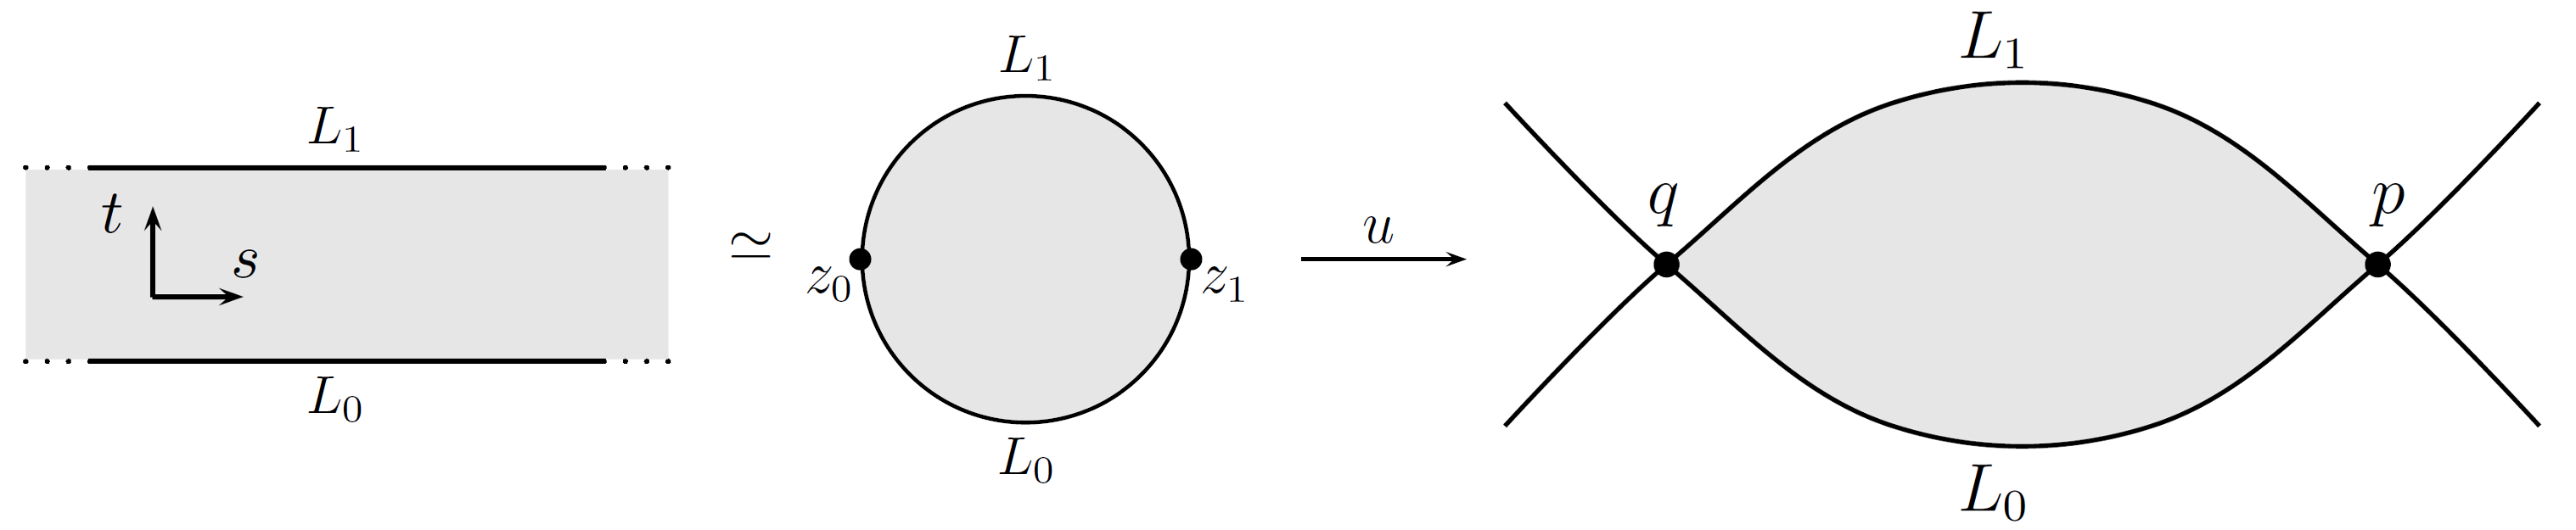
\includegraphics[width=0.9\linewidth]{fig02.png}
  \caption{属于 $\widehat{\mathcal M}(p,q;[u],J)$ 的一条 $J$-全纯条带 $u$。[来源：\cite{Aur13}]\hfill（原书 p.68）}
  \label{fig:02}
\end{figure}

\begin{Def}\label{def:5.12}
设 $M=(M,\omega,J)$ 是近复辛流形，$L_0,L_1\subset M$ 是紧致拉格朗日子流形，
且 $L_0\pitchfork L_1$。考虑 Cauchy--Riemann 问题 (57) 连同约束 (58) 与 (59)
的解 $u:\mathbb R\times[0,1]\to M$，它给出一个同伦类
$[u]\in\pi_2(M,L_0\cup L_1)
=\operatorname{Hom}_{\mathrm{hTop}}((B^2,S^1),(M,L_0\cup L_1))$，其中
$(B^2,S^1)\simeq(\mathbb D^2\setminus\{\pm1\},\mathbb R\times\{0\}\cup
\mathbb R\times\{1\})$ 与 $(M,L_0\cup L_1)$ 是带基点的拓扑空间对。

对固定的 $p,q\in\mathcal X(L_0,L_1)$，记
$\widehat{\mathcal M}(p,q;[u],J)$ 为表示 $[u]$ 的 (57)--(59) 之解构成的
\emph{模空间}，并令
$\mathcal M(p,q;[u],J):=\widehat{\mathcal M}(p,q;[u],J)/\mathbb R$。
\end{Def}

我们注意，$\mathbb R$ 通过沿 $s$ 坐标的平移自由作用在
$\widehat{\mathcal M}(p,q;[u],J)$ 上：若 $u(s,t)\in
\widehat{\mathcal M}(p,q;[u],J)$，则
$u_{\tilde s}(s,t):=u(s-\tilde s,t)\in\widehat{\mathcal M}(p,q;[u],J)$ 对所有
$\tilde s\in\mathbb R$ 成立。定义 $\mathcal M(p,q;[u],J)$ 时已把这一作用考虑在内。

现在有三方面问题妨碍我们为 $CF(L_0,L_1)$ 定义边界算子。也就是说，要使
$\widehat{\mathcal M}(p,q;[u],J)$ 成为“可驾驭”的空间，我们需要它具有如下性质：
\begin{itemize}
  \item \emph{横截性}，它保证 $\widehat{\mathcal M}(p,q;[u],J)$ 可被赋予有限维
  光滑流形的结构，其维数由 $[u]$ 的 Maslov 指标给出。
  \item \emph{紧致性}，只有在没有“能量堆积”使
  $\widehat{\mathcal M}(p,q;[u],J)$ 定义不良时才成立。
  \item \emph{可定向性}，它应与底拉格朗日子流形定向的选取相容。
\end{itemize}
然而，这些要求没有一项是先验满足的，因此需要额外假设。

先简要处理可定向性。下面的定义有意保持含糊，因为部分技术细节我们宁愿回避。
讲求实用的读者可以跳过。

\begin{Def}\label{def:5.13}
设 $L^n\subset M^{2n}$ 是拉格朗日子流形。假定 $L$ 可定向，即配有（一个等价类的）
处处非零 $n$-形式 $\theta_L\in\Omega^n(L)$，即一个体积形式。注意，由于光滑流形
特别是胞腔复形，可以考虑其骨架滤过。则称 $L$ 为：
\begin{itemize}
  \item \emph{自旋流形}，若可在 $1$-骨架 $L^{(1)}$ 上平凡化切丛 $TL$，且该平凡化
  可延拓到 $2$-骨架 $L^{(2)}$。这种平凡化的同伦类称为 $L$ 的\emph{自旋结构}；
  它存在当且仅当第二 Stiefel--Whitney 类
  $w_2(TL)\in H^2(L;\mathbb Z_2)$——$TL$ 的一个不变量——为零。
  \item 相对于某个固定 $\langle b\rangle\in H^2(M;\mathbb Z_2)$ 的
  \emph{相对自旋流形}，若 $w_2(TL)=\langle b\rangle|_L$。
\end{itemize}
\end{Def}

% [Tutor Note: 【含糊】定义 5.13 把自旋结构说成“$1$-骨架上可延拓到 $2$-骨架的
% 平凡化”，这只在胞腔复形上直观成立，严格定义须用 $TL$ 的 $2$-连通覆盖或
% $\operatorname{Spin}(n)$-主丛；相对自旋条件 $w_2(TL)=\langle b\rangle|_L$
% 则是为了在 $w_2(TM)\neq0$ 时仍能定向模空间。原文注明完整证明见
% \cite{Sei08} 第 12 章。]

假定 $L_0$ 与 $L_1$ 可定向且自旋，可以证明它们的自旋结构为
$\widehat{\mathcal M}(p,q;[u],J)$ 给出一个典范定向（\cite{Sei08} 第 12 章证明了
这一点）。不过，若 $\operatorname{char}(\mathbb K)=2$，这些假设都不必要。

\medskip
\noindent\fbox{\parbox{0.96\linewidth}{%
此后，我们总假定所有拉格朗日子流形都带有（隐含的）定向与自旋结构选取。}}
\medskip

\subsection{Maslov 指标}\label{sec:5.4}

同伦类 $[u]\in\pi_2(M,L_0\cup L_1)$（其中 $u$ 解 (57)--(59)）的 Maslov 指标
决定 $\widehat{\mathcal M}(p,q;[u],J)$ 的维数。实际情况其实更微妙（不熟悉此事的
读者可跳过下面这条注）：

\begin{Rem}\label{rem:5.14}
Cauchy--Riemann 问题 (57)--(59) 实际上是一个 \emph{Fredholm 问题}，即
$\bar\partial_J$ 在任一零点 $u$（即解）处的线性化 $D_{\bar\partial_J,u}$ 是
Fredholm 算子。可为 $[u]$ 指定其 \emph{Fredholm 指标}
$\operatorname{ind}([u]):=\dim(\ker(D_{\bar\partial_J,u}))
-\dim(\operatorname{coker}(D_{\bar\partial_J,u}))$，它实际上与下文将计算的
Maslov 指标一致。我们指出，哈密顿 Floer 理论实际上用另一个量来讨论，即
\emph{Conley--Zehnder 指标}。
\end{Rem}

回忆注 5.3 中拉格朗日 Grassmann 流形 $LGr(n)$ 的定义，它微分同胚于
$U(n)/O(n)$。可以证明，行列式映射 $\det:U(n)/O(n)\to S^1$ 的平方
$\det^2$ 诱导出同构 $\pi_1(LGr(n))\cong\pi_1(S^1)=\mathbb Z$。

\begin{Def}\label{def:5.15}
基于某个 $W\in LGr(n)$ 的环路 $\gamma:[0,1]\to LGr(n)$ 的\emph{Maslov 指标}
由 $\operatorname{im}(\det^2\circ\gamma)\subset S^1$ 的卷绕数
$\operatorname{ind}(\gamma):=w(\gamma,W)\in\mathbb Z$ 给出（这里把
$LGr(n)$ 等同于 $U(n)/O(n)$）。

另一方面，给定两条道路 $l_0,l_1:[0,1]\to LGr(n)$，满足
$l_0(0)\pitchfork l_1(0)$ 与 $l_0(1)\pitchfork l_1(1)$，定义
$l:=(l_0,l_1):t\in[0,1]\mapsto(l_0(t),l_1(t))\in LGr(n)\times LGr(n)$。
道路 $l_0,l_1$ 的\emph{Maslov 指标}是
\begin{equation}
\operatorname{ind}(l_0,l_1):=\left|\operatorname{im}(l)\cap
\overline{LGr(n)}\right|,
\label{eq:5.60}
\end{equation}
其中 $\overline{LGr(n)}:=\{(W,W')\in LGr(n)\times LGr(n)\mid
W\not\pitchfork W'\}$。换种说法，$\operatorname{ind}(l_0,l_1)$ 是
$l_0(t)$ 与 $l_1(t)$ 不横截的（带符号）次数，$0\le t\le1$ 递增。
\end{Def}

% [Tutor Note: 【易错】(60) 中横线并非闭包，而是“非横截对”之集：原文用
% $\overline{LGr(n)}$ 记 $\{(W,W')\mid W\not\pitchfork W'\}$，它是
% $LGr(n)\times LGr(n)$ 中余维 $1$ 的 Maslov 循环。$l$ 与该循环的相交数
% 带符号计数，符号由 $LGr(n)$ 的定向决定；这一符号约定经 (61)、(65) 一直
% 传到交点的次数 $\deg(p)$，故不能随意改动。]

让我们借助一个简单例子剖析指标对道路的几何意义。

\begin{Ex}\label{ex:5.16}
为简单起见，取 $l_0(t):=\mathbb R^n\subset\mathbb R^{2n}\cong\mathbb C^n$
为常值，并定义
$l_1(t):=(e^{i\varphi_1(t)}\mathbb R)\times\cdots\times
(e^{i\varphi_n(t)}\mathbb R)$，使所有角 $\varphi_k$ 一致地从 $-\pi/2$ 变到
$\pi/2$。$l_0$ 与 $l_1$ 的 Maslov 指标恰为
$\operatorname{ind}(l_0,l_1)=n$。这在 $n=1$ 时最易看出：此时 $l_0$ 是 $x$ 轴，
直线 $l_1(t)$ 逆时针地从 $l_1(0)=y$ 轴（其中 $\varphi_1(0)=-\pi/2$）转到
$l_1(1)=y$ 轴（其中 $\varphi_1(1)=\pi/2$），除 $\varphi(1/2)=0$ 时两条直线
实际重合外，其余时刻均与 $l_0$ 横截相交。\hfill$\blacklozenge$
\end{Ex}

现在考虑解 Cauchy--Riemann 问题 (57)--(59) 的 $J$-全纯条带
$u:\mathbb R\times[0,1]\to M$。对任意 $t\in[0,1]$，记
$q=u(-\infty,t)$ 与 $p=u(\infty,t)$。于是光滑映射 $u$ 给出辛拉回丛
$u^*TM=\{((s,t),(x,v))\in(\mathbb R\times[0,1])\times TM\mid u(s,t)=x\}$，
并可如下定义 $u$ 的 Maslov 指标。

\begin{Def}\label{def:5.17}
在为 $u^*TM\to\mathbb R\times[0,1]$ 选定平凡化之后（例如见 \cite{Mer14}
第 5 章），定义两条道路
$l_i(s):=((u|_{\mathbb R\times\{i\}})^*TL_i)|_{(-s,i)}
\cong T_{u(-s,i)}L_i$，其中 $s\in\overline{\mathbb R}=[-\infty,+\infty]$，
$i=0,1$；它们的像实际上落在 $LGr(n)$ 中（由注 5.3），并且每条 $l_i$ 都从
$T_pL_i$ 走向 $T_qL_i$，满足 $l_0(-\infty)\pitchfork l_1(-\infty)$ 与
$l_0(\infty)\pitchfork l_1(\infty)$（因为 $L_0\pitchfork L_1$）。

$J$-全纯条带 $u$ 的\emph{Maslov 指标}就是两条道路 $l_0,l_1$ 的 Maslov 指标，
$\operatorname{ind}([u]):=\operatorname{ind}(l_0,l_1)$，如定义 5.15 所述
（该定义对扩大的定义域 $\overline{\mathbb R}$ 仍然有效）。
\end{Def}

我们指出，$\operatorname{ind}(l_0,l_1)$ 实际上与 $u^*TM$ 所选取的平凡化无关，
且在 $\operatorname{Sp}(2n,\mathbb R)$ 中元素的共轭下不变。

% [Tutor Note: 【易错】定义 5.17 中 $l_i$ 的自变量是 $-s$，因此当 $s$ 从
% $-\infty$ 增至 $+\infty$ 时，$l_i$ 实际从 $T_pL_i$ 走向 $T_qL_i$。这一
% “反向参数化”是为与 (61) 中环路 $\gamma_u=\overline{l_0}*\lambda_p*l_1*
% \overline{\lambda_q}$ 的拼接次序配套；若漏掉负号，会得到
% $\operatorname{ind}([u])=\deg(p)-\deg(q)$ 而非推论 5.23 的结论。]

这使 $\operatorname{ind}([u])$ 良定义。此外，它在拼接下可加（进一步的性质以及
稍作修改的构造，见 \cite{Sei99} 第 4 节）。下面看它作为适当环路指标的等价表述。

\begin{Def}\label{def:5.18}
考虑 $\lambda_0,\lambda_1\in LGr(n)$，满足
$\lambda_0\pitchfork\lambda_1$。唯一确定变换
$A\in\operatorname{Sp}(2n,\mathbb R)$，使 $A(\lambda_0)=\mathbb R^n\subset
\mathbb C^n$ 且 $A(\lambda_1)=(i\mathbb R)^n\subset\mathbb C^n$。则称
$\lambda:t\in[0,1]\mapsto A^{-1}((e^{-i\pi t/2}\mathbb R)^n)\in LGr(n)$ 为从
$\lambda_0=\lambda(0)$ 到 $\lambda_1=\lambda(1)$ 的\emph{标准短路径}。
\end{Def}

\begin{Def}\label{def:5.19}
设 $u:\mathbb R\times[0,1]\to M$ 是解 Cauchy--Riemann 问题 (57)--(59) 的
$J$-全纯条带。按上一段定义道路 $l_0,l_1:\overline{\mathbb R}\to LGr(n)$，
并考虑如定义 5.18 的标准短路径
$\lambda_p,\lambda_q:[0,1]\to LGr(n)$，它们分别从 $T_pL_0$ 到 $T_pL_1$、
从 $T_qL_0$ 到 $T_qL_1$。

于是得到 $LGr(n)$ 中以 $T_qL_0$ 为基点的环路
$\gamma_u:=\overline{l_0}*\lambda_p*l_1*\overline{\lambda_q}$（横线表示逆道路）。
$u$ 的\emph{Maslov 指标}与相应的卷绕数一致：
\begin{equation}
\operatorname{ind}([u]):=\operatorname{ind}(\gamma_u)
=w(\gamma_u,T_qL_0)\,.
\label{eq:5.61}
\end{equation}
\end{Def}

\begin{Ex}\label{ex:5.20}
取 $M=\mathbb R^2$。则图 2 所示 $J$-全纯条带 $u$ 的 Maslov 指标可用如下技巧
计算：选取 $u^*TM$ 的平凡化，使道路 $l_0(s)=T_{u(-s,0)}L_0$ 等于常值切直线
$\mathbb R\times\{0\}$，并不失一般性地把 $L_1$ 参数化为向下的开口抛物线弧段
$\{(x,-x^2)\in\mathbb R^2\mid x\in[q,p]\}$（为清楚起见参看图 2）。

于是显然，道路 $l_1(s)=T_{u(-s,1)}L_1$ 只与 $l_0$ 不横截一次，即在 $s=0$ 处
（此处切线 $l_1(0)$ 平行于 $\mathbb R\times\{0\}$）。因此，按定义 5.19 用标准
短路径在 $T_qL_0$ 处闭合环路，便得 $\operatorname{ind}([u])=1$。
\hfill$\blacklozenge$
\end{Ex}

下面讨论如何为 Floer 复形配备 $\mathbb Z$-分次。这里，我们关于一阶 Chern 类
为 $2$-挠的假设开始发挥作用。

考虑纤维丛 $LGr(TM)\to M$，其纤维为
$LGr(TM)_x:=LGr(T_xM)\cong LGr(n)$（这是丛
$P\times_{\operatorname{Sp}(2n,\mathbb R)}LGr(n)$，其中 $P$ 是相伴的辛标架丛，
即 $M$ 上的主 $\operatorname{Sp}(2n,\mathbb R)$-丛），每个纤维都有万有覆盖
$\upsilon_x:\widetilde{LGr(T_xM)}\to LGr(T_xM)$。于是 $2c_1(TM)=0$ 让我们\footnote{遗憾的是，这又是一个超出本书范围的技术细节。它在
\cite{Fuk02b} 引理 2.6 或 \cite{Sei08} 第 (11j) 节中，在拉格朗日膜
（Lagrangian brane）的语境下得到处理。}可以把所有这些覆盖粘起来，形成覆盖空间
$\widetilde{LGr(TM)}\to LGr(TM)$，使得
$\widetilde{LGr(TM)}_x=\widetilde{LGr(T_xM)}$ 对所有 $x\in M$ 成立。
$\widetilde{LGr(TM)}$ 的元素称为 $TM$ 中的\emph{分次拉格朗日平面}。

现在，给定某条拉格朗日子流形 $L\subset M$ 上的截面
$s\in\Gamma(L,LGr(TM))$，$x\in L\mapsto T_xL\in LGr(T_xM)$，我们可能想问：
把 $s$ 提升为某个截面 $\tilde s\in\Gamma(L,\widetilde{LGr(TM)})$ 的障碍是什么？
也就是说，如何得到交换图
\begin{equation}
\begin{tikzcd}
& \widetilde{T_xL}\in\widetilde{LGr(T_xM)} \arrow[d,"\upsilon_x"] \\
x\in L \arrow[ur,"\tilde s"] \arrow[r,"s"'] & T_xL\in LGr(T_xM)
\end{tikzcd}
\label{eq:5.62}
\end{equation}
事实证明，我们需要 $L$ 的 Maslov 类消没：

\begin{Def}\label{def:5.21}
设 $(M,\omega)$ 是满足 $2c_1(TM)=0$ 的辛流形，于是可为每个
$W\in LGr(T_xM)$ 指定一个“相位” $\phi(W)\in S^1$，并选取提升
$\tilde\phi(W)\in\mathbb R$ 满足 $\phi(W)=e^{2\pi i\tilde\phi(W)}$。则对拉格朗日
子流形 $L\subset M$，可定义其“相位函数” $\phi_L:L\to S^1$，
$\phi_L(x):=\phi(T_xL)$。$L$ 的\emph{Maslov 类}恰为\footnote{注意，$\mathbb Z$
可除，故 $\operatorname{Ext}(H_0(L),\mathbb Z)$ 消没，从而
$H^1(L;\mathbb Z)\cong\operatorname{Hom}(H_1(L),\mathbb Z)$。又，在 $L$ 的连通
分支上，Hurewicz 定理告诉我们
$H_1(L)\cong\pi_1(L)^{\mathrm{ab}}=\pi_1(L)/[\pi_1(L),\pi_1(L)]$，而 $\mathbb Z$
交换保证 $\operatorname{Hom}(\pi_1(L),\mathbb Z)\cong
\operatorname{Hom}(\pi_1(L)^{\mathrm{ab}},\mathbb Z)$。}
\begin{equation}
\mu_L\equiv[\phi_L]:=\pi_1(\phi_L)\in\operatorname{Hom}(\pi_1(L),\pi_1(S^1))
\cong H^1(L;\mathbb Z)\,.
\label{eq:5.63}
\end{equation}
此外，选取映射 $\tilde\phi_L:L\to\mathbb R$ 提升 $\phi_L$，即使其落入交换图
\begin{equation}
\begin{tikzcd}
& \tilde\phi(T_xL)\in\mathbb R \arrow[d,"\exp(2\pi i\,\cdot\,)"] \\
x\in L \arrow[ur,"\tilde\phi_L"] \arrow[r,"\phi_L"'] & \phi(T_xL)\in S^1
\end{tikzcd}
\label{eq:5.64}
\end{equation}
便得到带有分次提升 $\tilde\phi_L$ 的\emph{分次拉格朗日子流形}
$(L,\tilde\phi_L)$。
\end{Def}

% [Tutor Note: 【含糊】原文说“可为每个 $W$ 指定相位 $\phi(W)\in S^1$”，其
% 依据是 $\det^2:U(n)/O(n)\to S^1$ 的万有覆盖；$2c_1(TM)=0$ 保证这些局部
% 相位能沿 $M$ 整体粘接。相位函数的提升 $\tilde\phi_L$ 一旦选定，交点的次数
% $\deg(p)$ 便确定；把 $\tilde\phi_L$ 整体平移整数 $k$，所有次数同时平移
% $k$，Floer 复形只作整体平移，上同调不变。]

现在选取横截相交的分次拉格朗日子流形
$(L_0,\tilde\phi_{L_0}),(L_1,\tilde\phi_{L_1})\subset M$，满足
$[\phi_{L_0}]=[\phi_{L_1}]=0$，于是存在如图 (62) 的截面。取任意
$p\in L_0\cap L_1$。则存在一条受偏爱的（同伦类的）道路
$l_p:[0,1]\to LGr(T_pM)$，使 $l_p(0)=T_pL_0$ 且 $l_p(1)=T_pL_1$，即覆盖映射
$\upsilon_p$ 在观察万有覆盖 $\widetilde{LGr(T_pM)}$ 后所选出的那一条。

\begin{Def}\label{def:5.22}
设 $(L_0,\tilde\phi_{L_0}),(L_1,\tilde\phi_{L_1})\subset M$ 是 Maslov 类消没的
分次拉格朗日子流形，$p\in L_0\cap L_1$。设 $l_p:[0,1]\to LGr(T_pM)$ 是上一段
所述道路，$\lambda_p:[0,1]\to LGr(T_pM)$ 是从 $T_pL_0$ 到 $T_pL_1$ 的标准短
路径。则 $p$ 的\emph{次数}由
\begin{equation}
\deg(p):=w(\gamma_p)
\label{eq:5.65}
\end{equation}
给出，其中 $\gamma_p:=l_p*\overline{\lambda_p}$ 是以 $T_pL_0$ 为基点的环路。
\end{Def}

在适当地等同切空间 $T_x(L_0\cap L_1)$ 之后，定义 5.19 与 5.22 的直接推论是：

\begin{Cor}\label{cor:5.23}
设 $u:\mathbb R\times[0,1]\to M$ 是解 Cauchy--Riemann 问题 (57)--(59) 的
$J$-全纯条带，其中 $L_0$ 与 $L_1$ 是横截相交、Maslov 类消没
（$[\phi_{L_0}]=[\phi_{L_1}]=0$）的分次拉格朗日子流形。则
\[
\operatorname{ind}([u])=\deg(q)-\deg(p).
\]
特别地，$\operatorname{ind}([u])$ 只依赖于由 $u$ 相连的两个生成元 $p,q$，
因此可为 $CF(L_0,L_1)$ 配备 $\mathbb Z$-分次：
\[
CF^n(L_0,L_1):=\bigoplus_{\substack{p\in\mathcal X(L_0,L_1):\\
\deg(p)=n}}\Lambda_{\mathbb K}\cdot p\,,
\qquad n\in\mathbb Z.
\]
\end{Cor}

% [Tutor Note: 【易错】推论 5.23 的符号取决于 (61) 的环路次序与 (58) 的端点
% 约定：$q$ 是负端（$s\to-\infty$）、$p$ 是正端（$s\to+\infty$），故
% $\operatorname{ind}=\deg(q)-\deg(p)$。若把 $u$ 反向参数化，得到的是
% $\deg(p)-\deg(q)$，这正是 (74) 中 $\partial$ 提升次数 $+1$ 的来源：
% 从 $p$ 到 $q$ 的条带使 $\deg(q)=\deg(p)+1$。]

若没有假设 $2c_1(TM)=0$ 与 $[\phi_{L_0}]=[\phi_{L_1}]=0$，我们仅得到
$\mathbb Z_2$-分次（这一替代方案在 \cite{Sei99} 第 4 节中简要讨论）。

\medskip
\noindent\fbox{\parbox{0.96\linewidth}{%
此后，我们假定所有（可定向自旋的）拉格朗日子流形都是分次的，且 Maslov 类消没。}}
\medskip

\subsection{横截性}\label{sec:5.5}

模空间 $\widehat{\mathcal M}(p,q;[u],J)$ 的横截性处理起来更具挑战性，尤其在
底层理论方面。

\begin{Rem}\label{rem:5.24}
沿用注 5.14 的技术要点：若线性化 $D_{\bar\partial_J,u}$ 的所有零点都是正则的，
即 $D_{\bar\partial_J,u}$ 对所有 $u\in\widehat{\mathcal M}(p,q;[u],J)$ 都满射，
则横截性得以实现。
\end{Rem}

$L_0\pitchfork L_1$ 情形的解决办法，是允许 $\omega$-相容近复结构依赖 $t$，
即把 (57) 中的 $J$ 换成 $J_t$，$t\in[0,1]$（形式上，取
$J\in C^\infty([0,1],\mathcal J(M,\omega))$ 并写 $J_t:=J(t,\,\cdot\,)$）。

当我们试图在最一般情形 $L_0\not\pitchfork L_1$ 下定义 $CF(L_0,L_1)$ 时，也会
遇到同样的策略——若想在 $CF(L_i,L_i)$ 中找到恒等态射，这种情形确实必须研究！
事实上，为摆脱拉格朗日子流形的横截性要求，我们考虑时间依赖的哈密顿函数
$H\in C^\infty([0,1]\times M)$，使得
$L_0\pitchfork(\phi_H^1)^{-1}(L_1)$，其中 $\phi_H^1:M\to M$ 是相应
$t$-依赖哈密顿向量场 $X_H\in\mathfrak X([0,1]\times M)$ 的哈密顿微分同胚。
于是方程 (57) 变成微扰 PDE，微扰由 $X_H$ 给出：
\begin{equation}
\bar\partial_{J,H}(u):=\partial_su+J_t(u)(\partial_tu-X_{H_t}(u))=0\,.
\label{eq:5.66}
\end{equation}
（这有时称为 \emph{Floer 方程}，$\bar\partial_{J,H}$ 称为 Floer 微分。）边界条件
必须相应修改。有限能量约束 (59) 成为：
\begin{equation}
E(u)=\frac12\int_{-\infty}^{+\infty}\!\!\int_0^1
\left(|\partial_su|^2+|\partial_tu-X_{H_t}(u)|^2\right)ds\,dt<\infty,
\label{eq:5.67}
\end{equation}
并且我们仍要求 $u(s,i)\in L_i$（$i=0,1$）。然而，$s\to\pm\infty$ 时的渐近线
因下面的观察而改变。

\begin{Rem}\label{rem:5.25}
微扰 Cauchy--Riemann 方程 (66) 可按如下方式化为 (57) 形式的齐次
Cauchy--Riemann 方程。设 $\phi_H^t:M\to M$ 是 $X_H$ 的流，并考虑 $u$ 在该流下
的原像 $\tilde u:\mathbb R\times[0,1]\to M$，
$\tilde u(s,t):=(\phi_H^t)^{-1}(u(s,t))$，于是链式法则给出
$\partial_t\tilde u=(\phi_H^t)^{-1}_*(\partial_tu-X_H)$。再定义
$\tilde J_t:=(\phi_H^t)^{-1}_*(J_t)$。则 (66) 呈现熟悉的面貌
\[
\partial_s\tilde u+\tilde J_t(\tilde u)\partial_t\tilde u=0,
\]
这是我们有把握其解为 $\tilde J$-全纯条带 $\tilde u$ 的 PDE，且
$\tilde u(s,0)=u(s,0)\in L_0$，
$\tilde u(s,1)=(\phi_H^1)^{-1}(u(s,1))\in(\phi_H^1)^{-1}(L_1)$。
\end{Rem}

% [Tutor Note: 【含糊】注 5.25 中“$\tilde J_t:=(\phi_H^t)^{-1}_*(J_t)$”是把
% 近复结构沿微分同胚拉回；要验证 $\tilde J_t$ 仍与某个辛形式相容，须同时
% 拉回 $\omega$ 或检查 $\tilde J_t^2=-\mathrm{id}$ 与相容性。原文未说明
% $(\phi_H^t)^{-1}_*$ 作用在 $(1,1)$-张量上，也未验证该拉回保持 $\tilde J$
% 的可积性以外的性质；这里照印，细节见 \cite{Mer14} 第 3 章。]

由上一注，Floer 复形的定义 5.11 现在需要修改
$\mathcal X(L_0,L_1)\equiv\mathcal X(L_0,L_1;H):=L_0\cap(\phi_H^1)^{-1}(L_1)$，
由于 $L_0\pitchfork(\phi_H^1)^{-1}(L_1)$，它仍是离散有限集。生成元是按流线
$\gamma:[0,1]\to M$（按定义满足 $\dot\gamma(t)=X_{H_t}(t,\gamma(t))$）微扰的
交点，使得 $\gamma(0)\in L_0$ 且 $\gamma(1)\in L_1$。相应地，Floer 微分计数
形如 $\mathcal M(p,q;[u],J,H)$ 的模空间中的\emph{微扰} $J$-全纯条带，这些模空间
现在也依赖于 $H$。

\begin{Rem}\label{rem:5.26}
（警告）在选取合适的 $H\in C^\infty([0,1]\times M)$ 使
$L_0\pitchfork(\phi_H^1)^{-1}(L_1)$ 时，我们忽略了一个非平凡事实：$H$ 实际上应
取自 $\mathcal H_{\mathrm{reg}}\subset C^\infty([0,1]\times M)$，即所有这样的
哈密顿函数之子集：其哈密顿微分同胚对某对拉格朗日子流形满足上述横截性。不过，
这并不使我们的分析失效，因为 $\mathcal H_{\mathrm{reg}}$ 原来是
$C^\infty([0,1]\times M)$ 的稠密子集（更精确地说，是 Baire 意义下的第二纲集；
参看 \cite{Sal97} 定理 1.24）。

类似地，保证线性化 $D_{\bar\partial_J,u}$ 满射（见注 5.24）的时间依赖近复结构
$J$，实际上也应属于稠密子集
$\mathcal J_{\mathrm{reg}}\subset C^\infty([0,1],\mathcal J(M,\omega))$。

选取数据 $(J,H)$ 时，我们把这些考虑放在心上。
\end{Rem}

% [Tutor Note: 【背景】$\mathcal H_{\mathrm{reg}}$ 稠密但不一定开；Floer 理论
% 的“通有选取”通常指存在稠密 $G_\delta$ 集使所有条带正则。原文用“Baire 第二
% 纲”表述，只保证稠密性，未保证稳定性；实际使用中还需横截性论证对每个
% 同伦类分别成立。]

让我们从略有不同的视角考察微扰问题 (66)，即 \cite{Oh91}、\cite{McS94} 与
\cite{Mer14} 第 3 章所提供的视角。

\begin{Def}\label{def:5.27}
设 $(M,\omega)$ 是辛流形，$L_0,L_1\subset M$ 是任意拉格朗日子流形，
$H\in C^\infty([0,1]\times M)$ 是时间依赖哈密顿量。定义\emph{道路空间}
\[
\mathcal P=\mathcal P(L_0,L_1):=\{\gamma\in C^\infty([0,1],M)\mid
\gamma(0)\in L_0,\ \gamma(1)\in L_1\}.
\]
这是具有可数多个连通分支的无穷维光滑流形，其切空间为
\[
T_\gamma\mathcal P=\Gamma(\gamma^*TM)\cong\Gamma_\gamma(TM)
:=\{\xi\in C^\infty([0,1],TM)\mid\xi(t)\in T_{\gamma(t)}M\},
\]
对每个 $\gamma\in\mathcal P$。我们通过它所等同的 $C^\infty(\mathcal P)$-线性映射
$\mathfrak X(\mathcal P)\to C^\infty(\mathcal P)$ 定义闭 $1$-形式
$a_H\in\Omega^1(\mathcal P)$：
\begin{equation}
\begin{aligned}
(a_H)_\gamma(\xi)
&:=\int_0^1\left(\omega_{\gamma(t)}(\xi(t),\dot\gamma(t))
-(dH_t)_{\gamma(t)}(\xi(t))\right)dt\\
&=\int_0^1\omega_{\gamma(t)}
\left(\xi(t),\dot\gamma(t)-X_{H_t}(\gamma(t))\right)dt,
\end{aligned}
\label{eq:5.68}
\end{equation}
其中 $\gamma\in\mathcal P$（于是
$\dot\gamma:=\frac{d}{dt}\big|_t\gamma\in\Gamma_\gamma(TM)$），
$\xi\in T_\gamma\mathcal P$；最后一个等式利用了
$dH_t=\omega(\,\cdot\,,X_{H_t}):\mathfrak X(M)\to C^\infty(M)$，即哈密顿向量场
的定义（见定义 5.4）。注意 $a_H$ 的闭性是 $\omega$ 闭性的直接推论。
\end{Def}

于是不难看出：

\begin{Cor}\label{cor:5.28}
设 $(M,\omega)$ 是辛流形，$L_0,L_1\subset M$ 是任意拉格朗日子流形，
$H\in C^\infty([0,1]\times M)$ 是生成流 $\phi_H^t:M\to M$ 的时间依赖哈密顿
函数。如上定义 $a_H\in\Omega^1(\mathcal P)$。则 $\gamma\in\mathcal P$ 是 $a_H$
的零点，$\gamma\in\operatorname{zeros}(a_H)$，当且仅当 $\gamma$ 是流线，即
$\gamma(t)=\phi_H^t(x)$ 对某个 $x\in L_0$ 成立。特别地，由时间 $0$ 处的求值给出
一个双射：
\begin{equation}
\{\gamma\in\operatorname{zeros}(a_H)\}\longleftrightarrow
\{\gamma(0)=x\in L_0\cap(\phi_H^1)^{-1}(L_1)\}\,.
\label{eq:5.69}
\end{equation}
\end{Cor}

推论 5.28 告诉我们，可以把 Floer 复形 $CF(L_0,L_1)$ 的生成元等同于闭
$1$-形式 $a_H$ 的零点；我们称后者为从 $L_0$ 到 $L_1$ 的\emph{时间 $1$ 哈密顿弦}。

不过，我们还能改进这一解释。

\begin{Def}\label{def:5.29}
设 $(M,\omega)$ 是辛流形，$L_0,L_1\subset M$ 是任意拉格朗日子流形。如上定义
道路空间 $\mathcal P=\mathcal P(L_0,L_1)$，并为
$\mathcal P=\bigsqcup_{k\in I}\mathcal P_k$ 的每个连通分支选取固定的参考道路
$\gamma_k\in\mathcal P_k$。对 $\gamma\in\mathcal P_k$，称\footnote{这一术语并非标准。}
$\bar\gamma\in C^\infty(\overline{\mathbb R}\times[0,1],M)$ 为
$\gamma$ 的\emph{桥}，若 $\bar\gamma(-\infty,\,\cdot\,)=\gamma_k$，
$\bar\gamma(+\infty,\,\cdot\,)=\gamma$，且
$\bar\gamma(s,\,\cdot\,)\in\mathcal P_k$ 对所有
$s\in\overline{\mathbb R}$ 成立（于是也可写
$\bar\gamma\in C^\infty(\overline{\mathbb R},\mathcal P_k)$）。
\end{Def}

\begin{Def}\label{def:5.30}
设 $(M,\omega)$ 是辛流形，$L_0,L_1\subset M$ 是拉格朗日子流形，
$H\in C^\infty([0,1]\times M)$。设 $\mathcal P=\mathcal P(L_0,L_1)$ 是相应的
道路空间，并固定某个 $\gamma_0\in\mathcal P$，使
$\gamma_0(0)=q\in L_0\cap(\phi_H^1)^{-1}(L_1)$ 是 Floer 复形
$CF(L_0,L_1)$ 的微扰生成元（或等价地由 (69)，使
$\gamma_0\in\operatorname{zeros}(a_H)$）。定义\emph{哈密顿作用量泛函}
$A_H:\mathcal P\to\mathbb R$ 为
\begin{equation}
A_H(\gamma):=\int_{\mathbb R\times[0,1]}\bar\gamma^*\omega
-\int_0^1H_t(\gamma(t))dt,
\label{eq:5.70}
\end{equation}
其中 $\bar\gamma\in C^\infty(\mathbb R\times[0,1],M)$ 是 $\gamma\in\mathcal P$ 的
任一桥，满足 $\bar\gamma(-\infty)=\gamma_0$（为使其有意义，注意 $\gamma$ 必须与
$\gamma_0$ 属于 $\mathcal P$ 的同一连通分支！）。
\end{Def}

就目前所写，$A_H$ 的定义仍不完整，因为我们必须证明它与桥 $\bar\gamma$ 的具体
选取无关——事实上我们小小地作弊了：若不对 $M,L_0,L_1$ 作适当假设，在
$\mathcal P=\mathcal P(L_0,L_1)$ 上定义哈密顿作用量泛函一般是不可能的，人们被迫
改在其 \emph{Novikov 覆盖} $\overline{\mathcal P}$ 上工作。这是由所有对
$[\gamma,\bar\gamma]$ 构成的空间，其中 $\bar\gamma$ 是 $\gamma\in\mathcal P$ 的
桥；在把相对于 $\partial(\mathbb R\times[0,1])$ 同伦的所有桥等同之后得到。再多做
一些工作，可以进一步改造 $\overline{\mathcal P}$，得到覆盖映射
$\pi:\overline{\mathcal P}\to\mathcal P$，在 $H=0$ 时满足
$dA_H=\pi^*(a_H)$（例如见 \cite{Oh91} 命题 13.5.1）。这在微扰情形 $H\neq0$ 下
仍然成立：

\begin{Lem}\label{lem:5.31}
设 $A_H:\overline{\mathcal P}\to\mathbb R$ 是哈密顿作用量泛函 (70)，
$a_H\in\Omega^1(\mathcal P)$ 是 $1$-形式 (68)。则
$dA_H=\pi^*(a_H)$。因此 $A_H$ 的临界点与 $a_H$ 的零点一致，
$\operatorname{crit}(A_H)=\operatorname{zeros}(a_H)$。
\end{Lem}

% [Tutor Note: 【易错】作用量泛函只在 Novikov 覆盖 $\overline{\mathcal P}$ 上
% 良定义，其理由与 (70) 中桥的选取有关：不同桥相差闭曲面，$\int\bar\gamma^*\omega$
% 的改变量是辛面积，一般非零。因此 $dA_H=\pi^*(a_H)$ 中的 $\pi^*$ 不可省；
% 原文在 $H=0$ 处说明，并称微扰情形同理。证明依赖 $\omega$ 闭与 Stokes 定理。]

这与推论 5.28 一起，帮助我们细化对一般 Floer 复形
$CF(L_0,L_1;H)$ 生成元的解释：
\begin{equation}
\{\gamma(0)=x\in\mathcal X(L_0,L_1;H)\}\longleftrightarrow
\{\gamma\in\operatorname{crit}(A_H)\}\,.
\label{eq:5.71}
\end{equation}

引理 5.31 还引出下面两个定义。

\begin{Def}\label{def:5.32}
设 $(M,\omega,J)$ 是近复辛流形，$J\in\mathcal J(M,\omega)$，
$L_0,L_1\subset M$ 是拉格朗日子流形，$H\in C^\infty([0,1]\times M)$。定义
$L^2$-内积
\[
\langle\!\langle\xi,\zeta\rangle\!\rangle_J
:=\int_0^1(g_J)_{\gamma(t)}(\xi(t),\zeta(t))dt
=\int_0^1\omega_{\gamma(t)}(J_{\gamma(t)}(\xi(t)),\zeta(t))dt,
\]
其中 $\gamma\in\mathcal P$，$\xi,\zeta\in T_\gamma\mathcal P$。然后记
$\nabla_JA_H\in\mathfrak X(\mathcal P)$ 为向量场
\begin{equation}
\nabla_JA_H(\gamma):=J(\gamma)(\dot\gamma-X_H(\,\cdot\,,\gamma))\in
T_\gamma\mathcal P
\label{eq:5.72}
\end{equation}
（其中 $J(\gamma)\equiv J_{\gamma(\,\cdot\,)}$）。显式地，对任意 $t\in[0,1]$ 有
$\nabla_JA_H(\gamma)(t):=J_{\gamma(t)}(\dot\gamma(t)-X_{H_t}(\gamma(t)))
\in T_{\gamma(t)}M$。
\end{Def}

\begin{Lem}\label{lem:5.33}
向量场 $\nabla_JA_H\in\mathfrak X(\mathcal P)$ 是 $A_H$ 关于
$\langle\!\langle\,\cdot\,,\,\cdot\,\rangle\!\rangle_J$ 的 $L^2$-梯度，即
$(dA_H)_\gamma(\xi)=\langle\!\langle\nabla_JA_H(\gamma),\xi\rangle\!\rangle_J$
对所有 $\gamma\in\mathcal P$ 与 $\xi\in T_\gamma\mathcal P$ 成立。
\end{Lem}

\begin{proof}
这是直接计算。取任意 $\gamma\in\mathcal P$ 与 $\xi\in T_\gamma\mathcal P$，则
\begin{align*}
(dA_H)_\gamma(\xi)
&=\int_0^1\omega_{\gamma(t)}\left(\xi(t),\dot\gamma(t)
-X_{H_t}(\gamma(t))\right)dt\\
&=\int_0^1\omega_{\gamma(t)}\left(J^2_{\gamma(t)}
\left(\dot\gamma(t)-X_{H_t}(\gamma(t))\right),\xi(t)\right)dt\\
&=\int_0^1(g_J)_{\gamma(t)}\left(J_{\gamma(t)}
\left(\dot\gamma(t)-X_{H_t}(\gamma(t))\right),\xi(t)\right)dt\\
&=\int_0^1(g_J)_{\gamma(t)}\left(\nabla_JA_H(\gamma)(t),\xi(t)\right)dt
=\langle\!\langle\nabla_JA_H(\gamma),\xi\rangle\!\rangle_J.
\end{align*}
\end{proof}

% [Tutor Note: 【易错】证明第二行用了 $J^2=-\mathrm{id}$ 与 $\omega$ 的反对称性：
% $\omega(J^2v,\xi)=\omega(-v,\xi)=\omega(\xi,v)$，故与第一行同值；第三行再用
% $g_J=\omega(J\,\cdot\,,\,\cdot\,)$。若采用文献中相反的 $g_J$ 约定，此处
% $\nabla_JA_H$ 与 (73) 的流方向都会整体变号。]

用刚刚建立的语言，微扰 Cauchy--Riemann 方程 (66) 可以写成
\begin{equation}
\frac{d}{ds}u(s)+\nabla_JA_H(u(s))=0,
\label{eq:5.73}
\end{equation}
这是 $\mathcal P$ 上的一个 ODE；其中我们把 $J$-全纯条带
$u:\mathbb R\times[0,1]\to M$ 重新解释为映射 $u:\mathbb R\to\mathcal P$，即
$A_H$ 的（有界）负梯度流线。解 $u\in\mathcal M(p,q;[u],J,H)$ 的能量可通过
作用量泛函表示为
\[
E(u)=A_H(\gamma_-)-A_H(\gamma_+),
\]
其中 $\gamma_\pm\in\operatorname{crit}(A_H)$ 满足 $\gamma_-(0)=q$ 与
$\gamma_+(0)=p$。显然这说得通：$\mathcal M(p,q;[u],J,H)$ 非空，当且仅当
$A_H(\gamma_-)>A_H(\gamma_+)$ 或 $\gamma_-=\gamma_+$。

然而，这一替代立场并未给我们带来更多好处，我们宁愿把焦点保持在\footnote{确实，这正是 Andreas Floer 在发展 Floer 同调时的天才直觉：把提法不当的 ODE (73) 看作 PDE (57) 的微扰，而 (57) 的解正是众所周知的 $J$-全纯条带。}$M$ 上的微扰
PDE (66)。对底层 Floer 理论机制感兴趣的读者，再次被引向 \cite{Oh91}。

\medskip
\noindent\fbox{\parbox{0.96\linewidth}{%
此后，我们隐含地选取时间依赖近复结构
$J\in C^\infty([0,1],\mathcal J(M,\omega))$ 与哈密顿量
$H\in C^\infty([0,1]\times M)$，把分析转向未必横截相交的拉格朗日子流形的
微扰 Cauchy--Riemann 问题 (66)。}}
\medskip

\subsection{紧致性}\label{sec:5.6}

在着手定义 Floer 微分之前，必须先处理光滑流形
$\widehat{\mathcal M}(p,q;[u],J,H)$ 的紧致性问题。由于下面这个结果（例如见
\cite{Sal97} 命题 3.3），它或许是第 5.3 节所列三项要求中最微妙的一项。

\begin{Pro}[Gromov 紧致性定理]\label{prop:5.34}
考虑一列 $J$-全纯条带
$(u_n)_{n\in\mathbb N}\subset\widehat{\mathcal M}(p,q;[u],J,H)$，其能量一致有界，
$\sup_{n\in\mathbb N}E(u_n)<\infty$。则存在有限多个点
$(s_j,t_j)\equiv s_j+it_j=:z_j\in\mathbb D^2\setminus\{\pm1\}$（例如
$j=1,\dots,l$），以及一个子列
$(u_{n_k})_{k\in\mathbb N}\subset\widehat{\mathcal M}(p,q;[u],J,H)$，它一致收敛
到 (66) 的某个解 $u\in\widehat{\mathcal M}(p,q;[u],J,H)$，且其导数在
$(\mathbb D^2\setminus\{\pm1\})\setminus\{z_1,\dots,z_l\}$ 的紧子集上收敛。
\end{Pro}

% [Tutor Note: 【含糊】Gromov 紧致性定理只说“在冒泡点之外 $C^\infty$ 收敛”，
% 既未说明极限对象是稳定映射（可能带气泡树），也未说明气泡的能量；证明需要
% 先验 $C^0$ 界、椭圆正则性与单调性，超出本书范围。原文把它当作黑箱使用，
% 并在 (75) 的粘接定理中反向补回。]

\begin{Def}\label{def:5.35}
考虑上一命题中 $J$-全纯曲线之子列
$(u_{n_k})_{k\in\mathbb N}\subset\widehat{\mathcal M}(p,q;[u],J,H)$。则导数
$(du_{n_k})_k$ 在那些 $z_j=(s_j,t_j)\in\mathbb R\times[0,1]$ 处无界，这造成
$k\to\infty$ 时的“能量集中”。我们说极限条带 $u$ 出现一个\emph{冒泡}。这种
“冒泡”现象有三种可能（见图 3）：
\begin{itemize}
  \item \emph{条带断裂}，发生在
  $\lim_{k\to\infty}|(du_{n_k})(z)|=\infty$ 于 $z=(s,t)\in\mathbb R\times[0,1]$
  且 $s\to\pm\infty$ 时，于是极限条带“断裂”（即具有一个中间节点）。若把每个
  分量看作 $J$-全纯圆盘，这等价于在端点 $p,q$ 之一处出现气泡。形式上，存在
  序列 $a_n\to\pm\infty$，使平移后的条带 $u_n(\,\cdot\,-a_n,\,\cdot\,)$ 收敛到
  一个非常值极限条带。
  \item \emph{圆盘冒泡}，发生在
  $\lim_{k\to\infty}|(du_{n_k})(z)|=\infty$ 于某个 $z=(s,t)\in\mathbb R\times
  [0,1]$、$t\in\{0,1\}$ 时，于是极限条带具有一个气泡，它由一张 $J$-全纯圆盘
  构成，其边界与 $L_0$ 或 $L_1$ 相交——并且在适当重标度后完全含于 $L_0$ 或
  $L_1$ 中。
  \item \emph{球面冒泡}，发生在
  $\lim_{k\to\infty}|(du_{n_k})(z)|=\infty$ 于某个
  $z=(s,t)\in(\mathbb R\times[0,1])^\circ$ 时，于是极限条带出现一个气泡，
  它在适当重标度后是一张 $J$-全纯球面 $\mathbb C P^1\to M$，并在
  $\operatorname{im}(u)$ 的某个内点处与其横截相交。
\end{itemize}
\end{Def}

条带断裂正是 Floer 微分在没有圆盘冒泡与球面冒泡时平方为零的原因。后两者不可取，
因为它们还妨碍 $\widehat{\mathcal M}(p,q;[u],J,H)$ 的横截性；第 5.5 节所采用的
微扰 $J\in C^\infty([0,1],\mathcal J(M,\omega))$ 与
$H\in C^\infty([0,1]\times M)$ 这次也解决不了问题！因此，我们希望保留条带断裂
现象，而舍弃圆盘冒泡与球面冒泡。\begin{figure}[htbp]
  \centering
  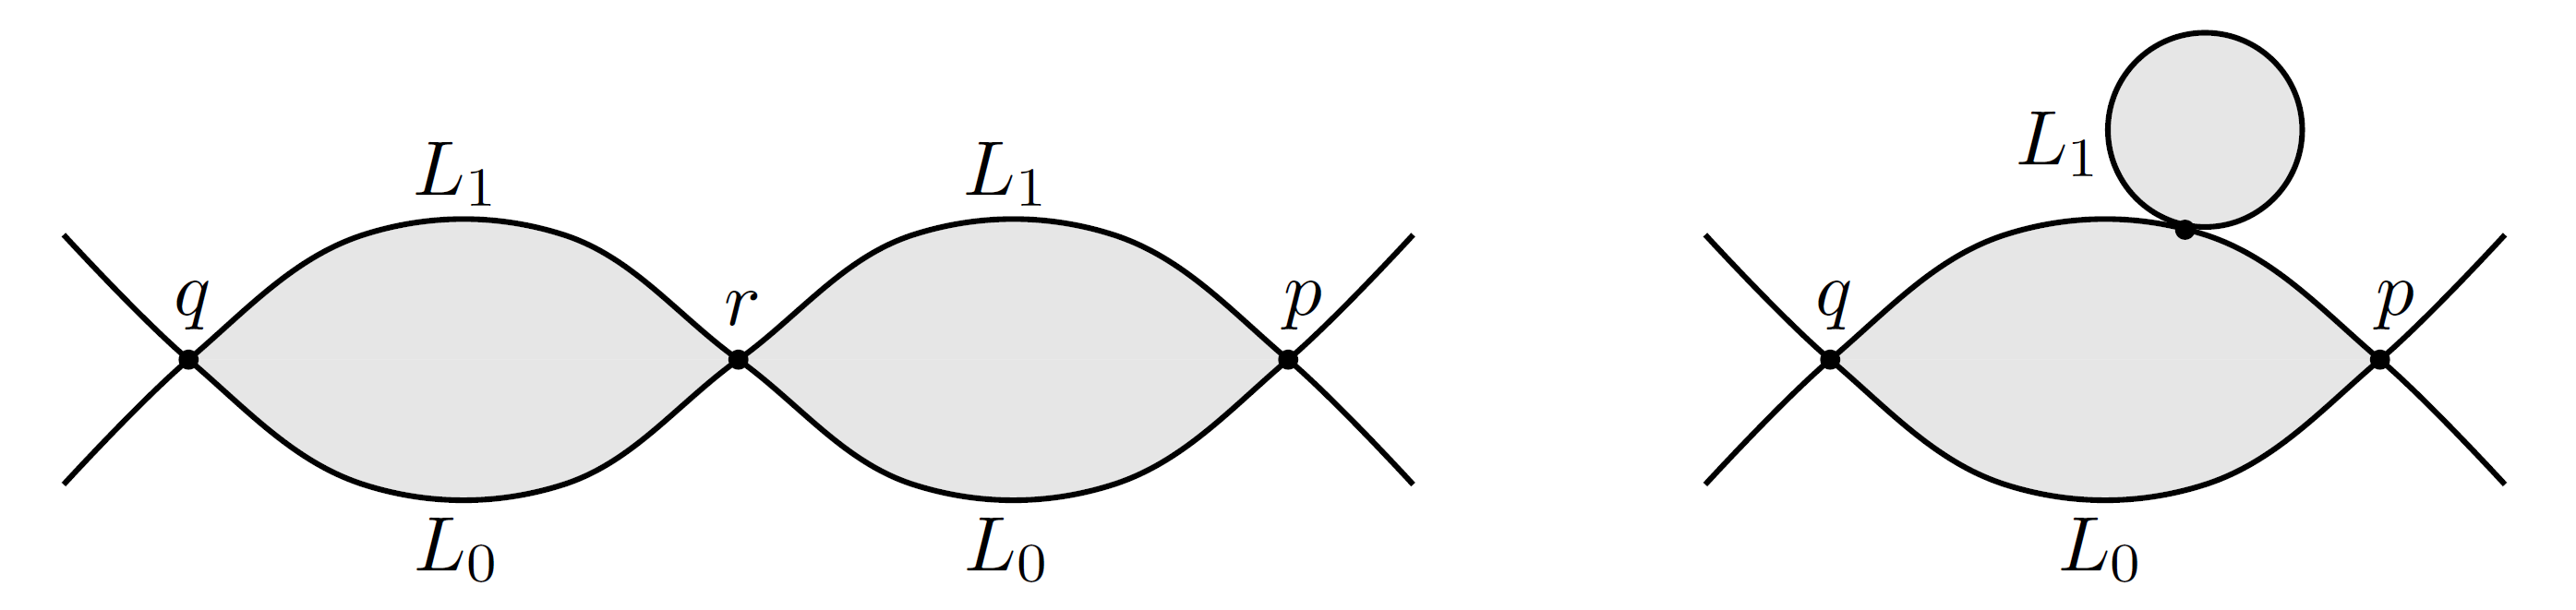
\includegraphics[width=0.9\linewidth]{fig03.png}
  \caption{两种可能的“冒泡”现象：条带断裂（左）与圆盘冒泡（右）。[来源：\cite{Aur13}]\hfill（原书 p.78）}
  \label{fig:03}
\end{figure}

这只需要求相应的 $J$-全纯圆盘与球面的辛面积
为零即可。

\begin{Lem}\label{lem:5.36}
设 $(M,\omega)$ 是辛流形，$L_0,L_1\subset M$ 是拉格朗日子流形，满足\footnote{注意
$\langle\omega\rangle\in H^2_{\mathrm{dR}}(M)\cong H^2(M;\mathbb R)\cong
\operatorname{Hom}(H_2(M),\mathbb R)\oplus\operatorname{Ext}(H_1(M),\mathbb R)
=\operatorname{Hom}(H_2(M),\mathbb R)$，于是把 $\pi_2(M)$ 与其在 Hurewicz 映射
$h:\pi_2(M)\to H_2(M)$ 下的像等同后，可把 $\langle\omega\rangle$ 限制到
$\pi_2(M)$。换言之，我们要求上同调与同调之间的配对
$\langle\langle\omega\rangle,h(\,\cdot\,)\rangle\equiv\langle\omega\rangle\cdot
\operatorname{im}(h)$ 消没，记号即由此而来。把 $\langle\omega\rangle$ 看作
$H^2_{\mathrm{dR}}(M,L_i)$ 的元素时同理。}
$\langle\omega\rangle\cdot\pi_2(M,L_i)=0$。则 $L_0$ 与 $L_1$ 不界定任何
$J$-全纯圆盘或球面。
\end{Lem}

% [Tutor Note: 【含糊】证明只有一行：若 $v:\mathbb D^2\to M$ 是边界落在 $L_i$
% 上的 $J$-全纯圆盘，则 $E(v)=\langle\omega,[v]\rangle=0$，故 $v$ 常值；球面
% 同理（因 $\pi_2(M)\to\pi_2(M,L_i)$）。原文未写出这一步，而它正是“面积为零”
% 与“无冒泡”等价的直观来源。]

这只是若干防止圆盘冒泡与球面冒泡的条件之一。后文将看到，在正合辛流形上，这一点
自动成立。

\medskip
\noindent\fbox{\parbox{0.96\linewidth}{%
此后，我们假定所有拉格朗日子流形 $L\subset M$ 都满足“无冒泡”条件
$\langle\omega\rangle\cdot\pi_2(M,L)=0$。}}
\medskip

\subsection{Floer 微分与 Floer 上同调}\label{sec:5.7}

我们终于收集齐了使后续理论适定的全部必要假设。下面着手定义 Floer 复形的第二份
数据。

\begin{Def}\label{def:5.37}
设 $(M,\omega)$ 是辛流形，$L_0,L_1\subset M$ 是拉格朗日子流形，相应的 Floer
复形 $CF(L_0,L_1)\equiv CF(L_0,L_1;J,H)$ 如 (56) 所定义（其中
$\mathcal X(L_0,L_1)=L_0\cap(\phi_H^1)^{-1}(L_1)$）。\emph{Floer 微分}
$\partial\equiv\partial_{J,H}:CF(L_0,L_1)\to CF(L_0,L_1)$ 是下式的
$\Lambda_{\mathbb K}$-线性延拓：
\begin{equation}
\partial(p):=\sum_{\substack{q\in\mathcal X(L_0,L_1)\\
[u]:\operatorname{ind}([u])=1}}
\left(\#\mathcal M(p,q;[u],J,H)\right)T^{\omega([u])}q,
\label{eq:5.74}
\end{equation}
其中 $\#\mathcal M(p,q;[u],J,H)\in\mathbb Z$（或 $\mathbb Z_2$）是来自微扰
Cauchy--Riemann 问题 (66) 的模空间 $\mathcal M(p,q;[u],J,H)$ 的（带符号或无符号）
基数，而 $\omega([u])$ 是辛面积（由无冒泡条件，它与代表元的选取无关）。由
推论 5.23，$\partial$ 的次数为 $1$。（注意 $\partial(p)$ 中 $q$ 的系数
\[
\sum_{[u]:\,\operatorname{ind}([u])=1}
\left(\#\mathcal M(p,q;[u],J,H)\right)T^{\omega([u])}\in\Lambda_{\mathbb K}
\]
是 Novikov 域的一个元素。）
\end{Def}

% [Tutor Note: 【易错】(74) 中 $T^{\omega([u])}$ 良定义依赖无冒泡条件：若
% $[u]$ 与 $[u']$ 同伦，则 $\omega([u])-\omega([u'])$ 是球面或带边圆盘的
% 面积，按假设为零。带符号计数 $\#\mathcal M$ 要求模空间可定向（定义 5.13 的
% 自旋结构），且 $\partial$ 提升次数 $+1$ 正是推论 5.23 的
% $\operatorname{ind}=\deg(q)-\deg(p)$。]

为证明 $\partial$ 良定义，还需要流形理论的最后一个（非平凡）结果。

\begin{Lem}\label{lem:5.38}
任意紧致 $1$ 维光滑流形 $M$ 的边界点的带符号总数等于零。
\end{Lem}

\begin{proof}
（略证）这是紧致 $1$ 维光滑流形分类定理的推论：任何这样的流形必微分同胚于有限
个闭实区间与若干 $S^1$ 拷贝的不交并。前者各有两个边界点，后者没有边界点。由于
边界点在微分同胚下保持，$M$ 有偶数个边界点。这直接证明了无符号计数的情形
（即模 $2$ 工作）。若我们关心定向、从而计入符号，仔细分析会揭示 $\partial M$ 的
带符号基数仍然相消。
\end{proof}

\begin{Thm}\label{thm:5.39}
设 $(M,\omega)$ 是辛流形，$L_0,L_1\subset M$ 是拉格朗日子流形，满足
$\langle\omega\rangle\cdot\pi_2(M,L_i)=0$（$i=0,1$）。则 $\partial$ 良定义，且
满足 $\partial^2=0$。此外，诱导的上同调群在选取时间依赖的 $J$ 与 $H$ 下
（在同构意义下）不变。
\end{Thm}

\begin{proof}
（略证）(74) 中的计数遍历所有同伦类
$[u]\in\pi_2(M,L_0\cup L_1)$，满足
$\operatorname{ind}([u])=\dim(\widehat{\mathcal M}(p,q;[u],J,H))=1$；于是相应的
模空间 $\mathcal M(p,q;[u],J,H)=\widehat{\mathcal M}(p,q;[u],J,H)/\mathbb R$
（由横截性它们是光滑流形）紧致、可定向且 $0$ 维，因而是可以带符号计数的有限集。
此外，(74) 中的和良定义，因为由 Gromov 紧致性定理，满足有限能量界 (67)、且其
模空间非空的同伦类 $[u]$ 只有有限多个。还要记得 $\mathcal X(L_0,L_1)$ 有限。

固定两个生成元 $p,q\in\mathcal X(L_0,L_1)$ 与某个 Maslov 指标为 $2$ 的
$[u]\in\pi_2(M,L_0\cup L_1)$。则
$\dim(\widehat{\mathcal M}(p,q;[u],J,H))=2$，于是光滑流形
$\mathcal M(p,q;[u],J,H)=\widehat{\mathcal M}(p,q;[u],J,H)/\mathbb R$ 是 $1$ 维的。
再次由命题 5.34，只需加入连接 $p$ 与 $q$、代表 $[u]$ 的断裂条带，便可把它紧化
为空间 $\overline{\mathcal M}(p,q;[u],J,H)$（按假设，没有陷入圆盘或球面冒泡的
风险）。相应地，其边界 $\partial\overline{\mathcal M}(p,q;[u],J,H)$ 含于形如
$\mathcal M(p,r;[u'],J,H)\times\mathcal M(r,q;[u''],J,H)$ 的模空间乘积之
不交并中，其中 $r\in CF(L_0,L_1)$ 是任意生成元，
$[u']+[u'']=[u]\in\pi_2(M,L_0\cup L_1)$（见图 3 左）。由于 Maslov 指标在条带
断裂下可加（按构造），且任何非常值条带的 Maslov 指标至少为 $1$（由横截性），
$\operatorname{ind}([u])=2$ 蕴含
$\operatorname{ind}([u'])=\operatorname{ind}([u''])=1$。反之，一个粘接定理\footnote{关于
某些有针对性的表述，可参看 \cite{Mer14} 第 8 节或 \cite{Sal97} 第 3.3 节，并思考
它们在 Morse 理论中的类比。}告诉我们，
$\overline{\mathcal M}(p,q;[u],J,H)$ 实际上是带边的 $1$ 维流形，且
\begin{equation}
\partial\overline{\mathcal M}(p,q;[u],J,H)
=\bigsqcup_{\substack{r\in\mathcal X(L_0,L_1)\\
[u']+[u'']=[u]\\
\operatorname{ind}([u'])=\operatorname{ind}([u''])=1}}
\mathcal M(p,r;[u'],J,H)\times\mathcal M(r,q;[u''],J,H),
\label{eq:5.75}
\end{equation}
其定向与各分量自然定向相容（后者来自 $L_0$ 与 $L_1$ 定向和自旋结构的隐含选取）。

由引理 5.38，紧致 $1$ 维光滑流形 $\mathcal M(p,q;[u],J,H)$ 的边界带符号基数
为零：
\[
\sum_{\substack{r\in\mathcal X(L_0,L_1)\\
[u']+[u'']=[u]\\
\operatorname{ind}([u'])=\operatorname{ind}([u''])=1}}
\left(\#\mathcal M(p,r;[u'],J,H)\right)\cdot
\left(\#\mathcal M(r,q;[u''],J,H)\right)=0.
\]
把最后一个表达式乘以 $\Lambda_{\mathbb K}$ 的形式变量 $T$、以总条带能量为权
$T^{\omega([u])}=T^{\omega([u'])+\omega([u''])}$，并对所有类
$[u]\in\pi_2(M,L_0\cup L_1)$ 求和，恰得 $\partial^2(p)$。因此 $\partial^2(p)=0$。

我们还须证明 $\partial=\partial_{J,H}$ 诱导的上同调群不依赖微扰数据 $J,H$ 的
选取。这里只给概览。\footnote{更多细节可在 \cite{Mer14} 第 9 章找到（非拉格朗日
情形）。}

取另一对 $(J',H')$。由于 $C^\infty([0,1],\mathcal J(M,\omega))$ 与
$C^\infty([0,1]\times M)$ 都道路连通，存在渐近常值道路
$\chi:\tau\in\overline{\mathbb R}\mapsto
(J(\tau),H(\tau))\in C^\infty([0,1],\mathcal J(M,\omega))\times
C^\infty([0,1]\times M)$，使得 $\chi(-\tau)=(J,H)$，且 $\chi(\tau)=(J',H')$
对所有 $\tau\ge N$ 成立，其中 $N\ge0$ 足够大。接着通过计数方程
\[
\partial_su+J_t(\tau,u)\left(\partial_tu-X_{H_t(\tau,u)}\right)=0
\]
的解来构造\emph{延拓映射}
$\Phi_\chi:CF(L_0,L_1;J,H)\to CF(L_0,L_1;J',H')$，方式如下：
$p'\in\mathcal X(L_0,L_1;H')$ 在 $F(p)$ 中的系数，是当
$s\to\pm\infty$ 时分别收敛到 $p$ 与 $p'$ 的指标 $0$ 解的带符号计数。对称地，
可定义延拓映射
$\Phi'_\chi:CF(L_0,L_1;J',H')\to CF(L_0,L_1;J,H)$。于是可以证明
$\partial_{J',H'}\circ\Phi_\chi=\Phi_\chi\circ\partial_{J,H}$ 与
$\partial_{J,H}\circ\Phi'_\chi=\Phi'_\chi\circ\partial_{J',H'}$，这意味着
$\Phi_\chi$ 与 $\Phi'_\chi$ 是互逆的链映射，从而
$\Phi'_\chi\circ\Phi_\chi$ 链同伦于
$\mathrm{id}_{CF(L_0,L_1;J,H)}$，而 $\Phi_\chi\circ\Phi'_\chi$ 链同伦于
$\mathrm{id}_{CF(L_0,L_1;J',H')}$。过渡到上同调便知
$H(\Phi_\chi):H(CF(L_0,L_1;J,H))\to H(CF(L_0,L_1;J',H'))$ 是同构，正如所求。
\end{proof}

% [Tutor Note: 【勘误】原文写 $\chi(-\tau)=(J,H)$ 且对 $\tau\ge N$ 有
% $\chi(\tau)=(J',H')$，其中 $\tau\in\overline{\mathbb R}$。按“渐近常值道路”
% 的通常含义应为：$\chi(\tau)=(J,H)$ 对 $\tau\le-N$，$\chi(\tau)=(J',H')$
% 对 $\tau\ge N$。译文照印原文，读者按此理解即可。]

% [Tutor Note: 【勘误】原文说 $p'$ 在“$F(p)$”中的系数，但 $F$ 在上下文里
% 没有定义；按文意应为延拓映射 $\Phi_\chi(p)$。译文照印 $F(p)$，读者按
% $\Phi_\chi(p)$ 理解即可。]

\begin{Def}\label{def:5.40}
设 $(M,\omega)$ 是辛流形，$L_0,L_1\subset M$ 是拉格朗日子流形，满足
$\langle\omega\rangle\cdot\pi_2(M,L_i)=0$（$i=0,1$）。则称
\begin{equation}
HF(L_0,L_1):=H(CF(L_0,L_1),\partial)=\frac{\ker(\partial)}
{\operatorname{im}(\partial)}
\label{eq:5.76}
\end{equation}
为\emph{拉格朗日 Floer 上同调}（由定理 5.39，可无歧义地选取任意
$J\in C^\infty([0,1],\mathcal J(M,\omega))$ 与 $H\in C^\infty([0,1]\times M)$
来定义 $CF(L_0,L_1)$ 与 $\partial$）。显式地，第 $n$ 个群为
$HF^n(L_0,L_1)=\ker(\partial_n)/\operatorname{im}(\partial_{n-1})$。
\end{Def}

由第 5.5 节的构造与定理 5.39 的证明立即推出：哈密顿同痕的拉格朗日子流形
$L_1,L_1'\subset M$ 在 Floer 上同调上诱导同构
$HF(L_0,L_1)\cong HF(L_0,L_1')$。另一方面，若 $L_0\cap L_1=\varnothing$，则
$HF(L_0,L_1)=\{0\}$。

\begin{Rem}\label{rem:5.41}
为得到 Floer \emph{同调}，必须把此前所有构造“反着”看。例如图 2 的条带从
$q$ 走向 $p$，最终导致所有分次反转。

回到上同调：在适当选取数据 $(J,H)$ 后，可以证明 Floer 复形
$CF(L_0,L_1)$ 与 $CF(L_1,L_0)$ 连同它们的微分互为对偶（此时从 $q$ 到 $p$ 的
条带是后者的一个元素）。
\end{Rem}

% [Tutor Note: 【易错】“上同调”与“同调”的差别不只是记法：把条带方向、端点
% 与 Maslov 指标同时反号后，$\partial$ 的次数从 $+1$ 变成 $-1$。原文的
% $HF(L_0,L_1)$ 是上同调，$\partial$ 提升次数；若按同调书写，需把整个复形
% 的指标取负，这正是注 5.41 所说“所有分次反转”。]

\begin{Ex}\label{ex:5.42}
看看放弃假设 $\langle\omega\rangle\cdot\pi_2(M,L_i)=0$ 会出什么问题，是有
启发性的；也就是说，允许拉格朗日子流形界定 $J$-全纯圆盘与球面。考虑 $2$ 维
流形 $M:=\mathbb R\times S^1$，带标准面积形式 $\omega:=ds\wedge dt$，以及
图 4 左所示的拉格朗日子流形 $L_0,L_1$。则 $L_0$ 与 $L_1$ 界定两张 Maslov
指标为 $1$ 的 $J$-全纯条带 $u,v$，它们分别从 $p$ 到 $q$、从 $q$ 到 $p$。按
定义，$\partial(p)=\pm T^{\omega([u])}q$ 且
$\partial(q)=\pm T^{\omega([v])}p$，于是
$\partial^2(p)=\pm T^{\omega([u])+\omega([v])}p\neq0$。
\end{Ex}

\begin{figure}[htbp]
  \centering
  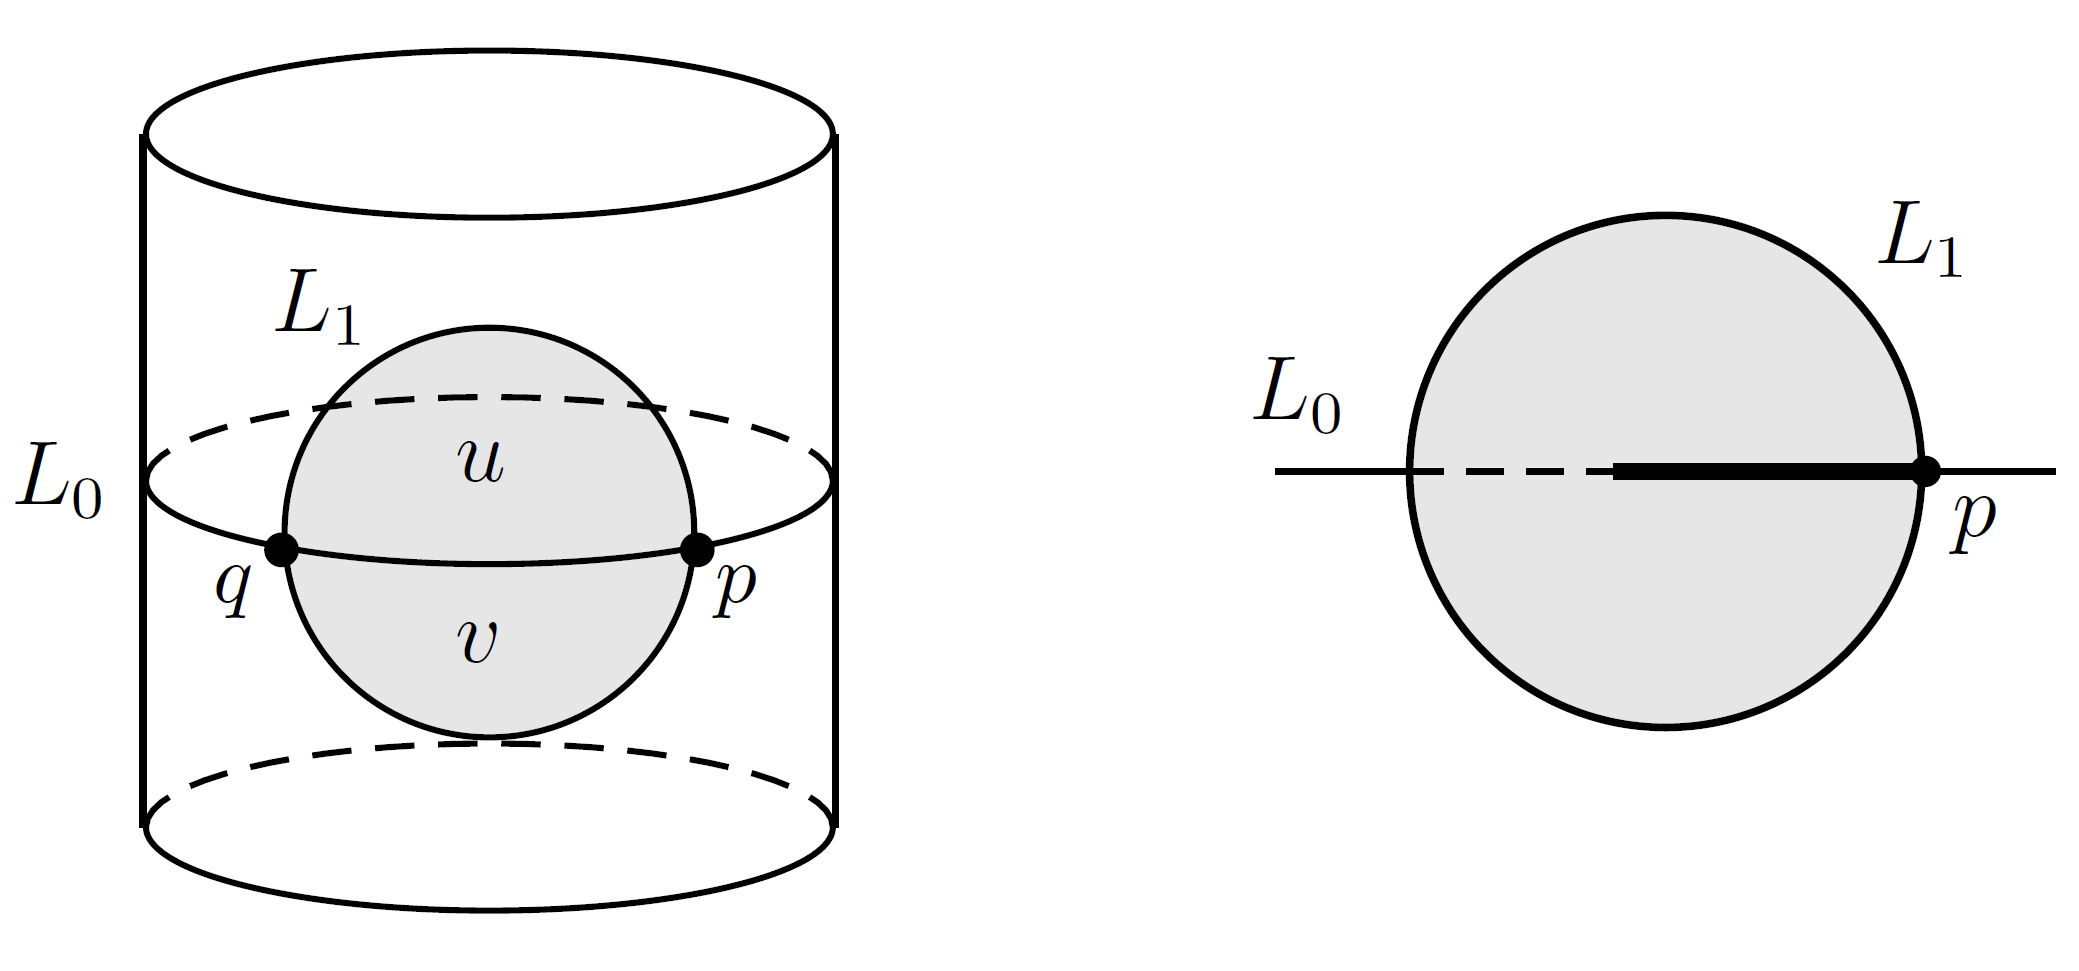
\includegraphics[width=0.8\linewidth]{fig04.png}
  \caption{若拉格朗日子流形上存在 $J$-全纯圆盘，则 Floer 微分不再平方为零。[来源：\cite{Aur13}]\hfill（原书 p.81）}
  \label{fig:04}
\end{figure}

从代数上看发生了什么？看图 4 右中 $M$ 的局部图像，在把
$\mathbb R\times[0,1]\simeq\mathbb D^2\setminus\{\pm1\}\subset\mathbb C$ 等同
之后，$L_0\supset[-1,1]$ 落在 $\mathbb R$ 上，而 $L_1$ 与 $S^1$ 重合。聚焦于
从 $p$ 到自身的指标 $2$ 的 $J$-全纯条带模空间，其像可通过沿 $L_0$（图中粗线）
剪开一条缝得到。任何这样的条带由
\[
w_\alpha(z):=\frac{z^2+\alpha}{1+\alpha z^2},
\qquad\text{其中}\quad
dw_\alpha(z)=2z\,\frac{1-\alpha^2}{(1+\alpha z^2)^2},
\]
给出，$\alpha\in(-1,1)$ 调节缝长。有两种极限情形：
\begin{itemize}
  \item 若 $\alpha\to-1$，指标 $2$ 的条带 $(w_\alpha)_\alpha$ 收敛到断裂条带
  $w$，其指标 $1$ 的分量为 $u$ 与 $v$，正如 图 3 左（确实，我们可以沿缝把
  图 4 的圆盘“打开”，并微分同胚地映为断裂构型）。这意味着能量集中在
  $z=\pm1$，正如以下所确认：
  \[
  \lim_{\alpha\to-1}|dw_\alpha(\pm1)|
  =\lim_{\alpha\to-1}\left|\frac{-4\alpha}{2(1+\alpha)}\right|=\infty.
  \]
  \item 若 $\alpha\to1$，$(w_\alpha)_\alpha$ 收敛到 $p$ 处的常值条带，并在
  $z=i$ 处带一个圆盘气泡，映到 $L_1$ 所围成的圆盘。于是能量集中在 $i$：
  \[
  \lim_{\alpha\to1}|dw_\alpha(i)|
  =\lim_{\alpha\to1}\left|\frac{4\alpha}{2(1-\alpha)}\right|=\infty.
  \]
\end{itemize}
$\alpha\to1$ 时发生的圆盘冒泡导致 $\partial^2(p)\neq0$！
\hfill$\blacklozenge$

% [Tutor Note: 【勘误】直接计算给出
% $|dw_\alpha(\pm1)|=2(1-\alpha)/(1+\alpha)$、
% $|dw_\alpha(i)|=2(1+\alpha)/(1-\alpha)$，而原文两式
% $\left|-4\alpha/(2(1+\alpha))\right|$、$\left|4\alpha/(2(1-\alpha))\right|$
% 与它们相差一个因子 $2$（且前者符号不同）。两式都仍趋于 $\infty$，故
% “能量集中”的结论不受影响；译文照印原文。]

% [Tutor Note: 【背景】例 5.42 说明：圆盘冒泡使 $\partial^2\neq0$，Floer 上
% 同调在一般辛流形上并非总是定义良好，除非引入 Kuranishi 结构/虚拟技术
% （\cite{FOOO09}）。这正是第 5.8 节转向正合流形、以及第 6 章引入 wrapped
% Fukaya 范畴的动机之一。]

最后，描述 $L_0=L_1$ 情形的 Floer 上同调。同样，以下陈述的证明对我们这个层次
来说相当高级——它涉及 Morse 理论——因此只给略证，并把读者引向 \cite{Aur13}
例 1.12。

\begin{Pro}\label{prop:5.43}
设 $(M^{2n},\omega)$ 是辛流形，$L^n\subset M$ 是拉格朗日子流形，满足
$\langle\omega\rangle\cdot\pi_2(M,L)=0$。则
$HF(L,L)\cong H(L;\Lambda_{\mathbb K})$（系数在 Novikov 域中的奇异上同调）。
\end{Pro}

\begin{proof}
（略证）首先，设 $L$ 是任意紧致实 $n$ 维流形。已知\footnote{由 Weinstein
拉格朗日邻域定理；见 \cite{Sil12} 定理 8.4。}$L\subset M$ 的某个邻域辛同胚于
$L_0:=\mathbf o(L)\subset T^*L$ 的某个邻域，其中
$\mathbf o\in\Gamma(L,T^*L)$ 表示零截面，而
$T^*L=(T^*L,\theta=\sum_i dq_i\wedge dp_i)$ 是 $L$ 的余切丛。取 Morse 函数
$f\in C^\infty(L)$ 与某个 $\varepsilon>0$，令
$L_1:=\operatorname{graph}(\varepsilon df)
=\{(x,\varepsilon(df)_x)\in T_x^*L\mid x\in L\}$。则
$L_0,L_1\subset T^*L$ 是哈密顿同痕的正合拉格朗日子流形，在
$\operatorname{crit}(f)$（即 $f$ 的临界点集）处横截相交。

选取分次提升，得到分次 Floer 复形 $CF(L_0,L_1)$，其生成元为任意
$p\in\operatorname{crit}(f)$，且 $\deg(p)=n-i(p)$（$i(p)$ 为 $p$ 的 Morse
指标）。经过适当的微扰与重标度，可以证明
$HF(L_0,L_1)\cong HM(f;\Lambda_{\mathbb K})$，即 $L$ 的 Morse 上同调，而后者
又同构于通常的奇异上同调 $H(L;\Lambda_{\mathbb K})$。连同哈密顿同痕下的不变性，
便得 $HF(L,L)\cong HF(L_0,L_0)\cong HF(L_0,L_1)\cong H(L;\Lambda_{\mathbb K})$。

现在设 $L^n\subset M$ 是满足 $\langle\omega\rangle\cdot\pi_2(M,L)=0$ 的
拉格朗日子流形。对足够小的微扰哈密顿量，决定 $HF(L,L)$ 的任何 $J$-全纯条带
必含于 $L$ 的某个小管状邻域中（由于能量约束）。因此上述分析也适用于这一般
情形。
\end{proof}

% [Tutor Note: 【勘误】原文把余切丛写成
% $T^*L=(T^*L,\theta=\sum_i dq_i\wedge dp_i)$；但 $\theta$ 应是一次形式
% （Liouville 形式 $\theta=\sum_i p_i\,dq_i$），而 $\sum_i dq_i\wedge dp_i$
% 是辛形式 $\omega_{T^*L}$（二次形式）。疑为笔误。译文照印原文；读者应以
% $\theta=\sum_i p_i\,dq_i$、$\omega=-d\theta=\sum_i dq_i\wedge dp_i$ 为准。]

% [Tutor Note: 【易错】$\deg(p)=n-i(p)$ 中 $i(p)$ 是 Morse 指标（负特征值
% 个数），故临界点的次数与 Morse 上同调的次数一致；若改用 Morse 同调（把
% 指标当作次数），所有次数变成 $i(p)$，与推论 5.23 的次数相差 $n$ 的平移。
% 这一平移是 $L$ 的分次提升选取的一部分，不影响 $HF(L,L)\cong H(L;\Lambda)$
% 的结论。]

% [Tutor Note: 【含糊】“经过适当的微扰与重标度”一句省略了关键步骤：需要把
% 条带方程在 $L$ 的管状邻域内展开，并证明只在 $\operatorname{crit}(f)$ 附近
% 有解（能量限制在小常数以下），从而把 Floer 微分与 Morse 微分逐项等同；
% 细节见 \cite{Aur13} 例 1.12 与 \cite{Sei08} 第 17 章。原文只说“可以证明”。]

再次强调，无冒泡假设 $\langle\omega\rangle\cdot\pi_2(M,L)=0$ 是本质的：否则
$HF(L,L)$（只要它有定义）可能只是 $H(L;\Lambda_{\mathbb K})$ 的一个更小的子群。

\subsection{正合流形情形}\label{sec:5.8}

在继续之前，让我们在正合辛流形 $M$ 中存在正合拉格朗日子流形 $L$ 的情形下，
简要重访上一节的理论。和以前一样，假定 $2c_1(TM)=0$，且所有 $L$ 都是紧致、
可定向、自旋、分次的，并具有消没的 Maslov 类。

\begin{Lem}\label{lem:5.44}
设 $(M^{2n},\omega)$ 是正合辛流形，$L_0,L_1\subset M$ 是正合拉格朗日子流形。
则定义 $CF(L_0,L_1)$ 的任何 $J$-全纯条带的能量为常数。此外，圆盘冒泡与球面
冒泡现象不会发生（即使我们不要求 $\langle\omega\rangle\cdot\pi_2(M,L_i)=0$！）。
\end{Lem}

\begin{proof}
设 $\omega=d\nu\in\Omega^2(M)$ 是附着于 $M$ 的正合形式，其中
$\nu\in\Omega^1(M)$；并设 $f_i\in C^\infty(L_i)$ 满足
$\nu|_{L_i}=df_i\in\Omega^1(L_i)$（$i=0,1$，参看定义 5.2）。考虑从 $p$ 到
$q$、边界在 $L_0\cup L_1$ 中的 $J$-全纯条带 $u:\mathbb R\times[0,1]\to M$，
如图 2 所示。其能量为
\begin{equation}
\begin{aligned}
E(u)&=\int_{\mathbb R\times[0,1]}u^*\omega
=\int_{\mathbb R\times[0,1]}d(u^*\nu)
&&\text{（因 $d$ 与拉回可交换）}\\
&=\int_{\partial(\mathbb R\times[0,1])}u^*\nu
&&\text{（由 Stokes 定理）}\\
&=\int_{\mathbb R\times\{1\}}u^*(\nu|_{L_1})
-\int_{\mathbb R\times\{0\}}u^*(\nu|_{L_0})
&&\text{（因 $\mathbb R\times\{i\}$ 映入 $L_i$）}\\
&=\int_{\mathbb R\times\{1\}}d(u^*f_1)
-\int_{\mathbb R\times\{0\}}d(u^*f_0)
&&\text{（因 $d$ 与拉回可交换）}\\
&=\int_{\partial(\mathbb R\times\{1\})}f_1\circ u
-\int_{\partial(\mathbb R\times\{0\})}f_0\circ u
&&\text{（由 Stokes 定理与 $u^*$ 的定义）}\\
&=\left.f_1(u(\,\cdot\,,1))\right|_{+\infty}^{-\infty}
-\left.f_0(u(\,\cdot\,,0))\right|_{+\infty}^{-\infty}
&&\text{（因我们从 $p$ 积分到 $q$）}\\
&=(f_1(q)-f_1(p))-(f_0(q)-f_0(p)).
\end{aligned}
\label{eq:5.77}
\end{equation}
因此 $u$ 的能量为常数，正如所断言。

现在考虑可能的冒泡现象。若 $v:\mathbb D^2\to M$ 是 $J$-全纯圆盘，其像在
某点 $r\in L_1$ 处与 $u$ 相交（见图 3 右），则其能量为
\[
E(v)=\int_{\mathbb D^2}v^*\omega=\int_{S^1}v^*\nu
=\int_{\partial S^1}v^*f_1=0
\]
（利用 $d$ 与 $v^*$ 可交换、两次使用 Stokes 定理，以及
$\partial S^1=\varnothing$）。类似地，设 $w:\mathbb C P^1\simeq S^2\to M$ 是
$J$-全纯球面，在某个内点处与 $u$ 相交。相应能量为
\[
E(w)=\int_{S^2}w^*\omega=\int_{\partial S^2}w^*\nu=0
\]
（因 $\partial S^2=\varnothing$）。由此可见，在两种情形下，条带的任何区域都
没有奇异的能量集中。因此圆盘冒泡与球面冒泡被排除。
\end{proof}

% [Tutor Note: 【易错】计算 (77) 时，$\partial(\mathbb R\times[0,1])$ 的
% 定向为 $\mathbb R\times\{1\}$ 取正向、$\mathbb R\times\{0\}$ 取负向，故
% 第三行两项符号相反；而 $u(+\infty)=p$、$u(-\infty)=q$，所以
% $f_1(u)|^{+\infty}_{-\infty}$ 的上限是 $+\infty$、下限是 $-\infty$。原文
% 写成 $|^{+\infty}_{-\infty}$ 却得 $f_1(q)-f_1(p)$，是因为其竖线记号的
% 上下限顺序与常规相反；译文照印，计算以 (77) 末行为准。]

% [Tutor Note: 【易错】(77) 末行不一定是正数：$E(u)\ge0$ 给出
% $(f_1(q)-f_1(p))\ge(f_0(q)-f_0(p))$，即 $f_1-f_0$ 沿条带从 $p$ 到 $q$
% 不增。这一单调性与 $E(u)=A_H(\gamma_-)-A_H(\gamma_+)$ 一致，也是
% “正合情形无冒泡”的真正原因：任何非定常圆盘或球面的能量必为零。]

因此，若与正合拉格朗日子流形打交道，使 Floer 微分良定义所需的紧致性便自动
获得。不过，若 $M$ 非紧，则需对其加一个额外假设（具体地说，$M$ 必须在无穷远
处凸，或者几何有界；例如参看 \cite{CGK02}）。又，借助方程 (77)——它告诉我们
所有辛面积都相等——可用因子 $T^{f_1(p)-f_0(p)}$ 重标度生成元
$p\in\mathcal X(L_0,L_1)$，从而 (74) 中的权重 $T^{\omega([u])}$ 可被忽略，允许
我们直接在域 $\mathbb K$ 上工作。

% [Tutor Note: 【易错】重标度的具体做法是：把生成元 $p$ 换成
% $T^{f_1(p)-f_0(p)}p$，则 (74) 中 $q$ 的系数变为
% $T^{\omega([u])+f_1(q)-f_0(q)}$；由 (77)，
% $\omega([u])=f_1(q)-f_1(p)-f_0(q)+f_0(p)$，故该指数恰为
% $f_1(p)-f_0(p)$，与 $p,q$ 之外的量无关，可整体提出。这样 $\partial$ 与
% 原来的只差一个对角共轭，上同调不变。]

最重要的是，引理 5.44 告诉我们，正合拉格朗日子流形不可能被阻碍，于是其中每
一个都是 Fukaya 范畴的（非零）对象。下面总结这一情形。

\begin{Def}\label{def:5.45}
设 $(M,\omega)$ 是正合辛流形，配有某个
$J\in C^\infty([0,1],\mathcal J(M,\omega))$ 与
$H\in C^\infty([0,1]\times M)$。设 $L_0,L_1\subset M$ 是正合拉格朗日子流形
（带有上文列出的全部数据）。$(L_0,L_1)$ 的 \emph{Floer 复形}是自由模
\[
CF(L_0,L_1)\equiv CF(L_0,L_1;H):=
\bigoplus_{p\in L_0\cap(\phi_H^1)^{-1}(L_1)}\mathbb K\cdot p,
\]
连同边界算子 $\partial\equiv\partial_{J,H}:CF(L_0,L_1)\to CF(L_0,L_1)$；后者
定义为下式的 $\mathbb K$-线性延拓：
\[
\partial(p):=\sum_{\substack{q\in L_0\cap(\phi_H^1)^{-1}(L_1)\\
[u]:\operatorname{ind}([u])=1}}
\left(\#\mathcal M(p,q;[u],J,H)\right)q
\]
（若希望忽略定向，只需作替换 $\mathbb K\leftarrow\mathbb Z_2$ 与
$\#\mathcal M(p,q;[u],J,H)\leftarrow
|\mathcal M(p,q;[u],J,H)|\ (\mathrm{mod}\ 2)$）。我们得到拉格朗日 Floer 上同调
$HF(L_0,L_1):=H(CF(L_0,L_1;H),\partial_{J,H})$；由定理 5.39 知它与
$(J,H)$ 的选取无关。
\end{Def}



% ============================================================================
% 第 6 章  Fukaya 范畴  （原书 pp.85–109，PDF pp.88–112）
% ============================================================================
\section{Fukaya 范畴}\label{ch:06}

% 原书公式在全书范围内连续编号：本章自 (78) 起、至 (100) 止，共 23 个编号公式。
% main.tex 已采用全局连续编号；此处补设计数器为 77，保证本章首个编号公式
% 恰为 (78)。若前几章的公式计数已经连续到 77，则本行只是空操作。
\setcounter{equation}{77}

\takeaway{%
  核心图像：Fukaya 范畴以拉格朗日子流形为对象、以 Floer 复形为态射空间，
  合成映射 $\mu^d$ 由伪全纯多边形的带权计数给出；对象间的“几何运算”
  （映射锥）具体化为 Dehn 扭转与拉格朗日连通和。\\
  数学工具：伪全纯圆盘与条带的模空间、Maslov 指标、结合面体 $K_d$、
  非幺 $A_\infty$-范畴、扭复形与 Yoneda 嵌入。\\
  主要结论：$\mu^d$ 满足 $A_\infty$-结合关系（命题 6.12），上同调范畴与
  三角包络分别是 Donaldson–Fukaya 范畴与 $\mathsf D^\pi(\mathcal F(M))$；
  沿球面的 Dehn 扭转与沿单点横截相交的连通和都等于映射锥
  （定理 6.23、定理 6.28）；wrapped 版本以卷绕哈密顿量处理非紧正合流形。%
}

\subsection{Floer 乘积}\label{sec:6.1}

我们引入第三条拉格朗日子流形，并改造上一章的几何构造，以便在两个 Floer
复形之间定义一个乘积，即 \emph{Floer 乘积}。主要参考文献是 \cite{Aur13}
第 2 节。

照例考虑近复辛流形 $M^{2n}=(M,\omega,J)$，其中 $2c_1(TM)=0$ 且
$J\in\mathcal J(M,\omega)$；再取三条拉格朗日子流形 $L_0,L_1,L_2\subset M$，
假定它们紧致、可定向、自旋、分次，Maslov 类消没，且不包围任何冒泡。
此外设它们两两横截相交：$L_i\pitchfork L_j$ 对 $i\neq j\in\{0,1,2\}$ 成立。
此时横截性、紧致性与可定向性都容易实现（一般情形稍后讨论）。我们要找的
是相应 Floer 复形之间如下形式的乘积运算：
\[
CF(L_1,L_2)\otimes CF(L_0,L_1)\longrightarrow CF(L_0,L_2)\,.
\]

参照图~\ref{fig:05}，研究如下问题：给定 $p_1\in\mathcal X(L_0,L_1)$、
$p_2\in\mathcal X(L_1,L_2)$、$q\in\mathcal X(L_0,L_2)$（此处暂时
$\mathcal X(L_i,L_j)=L_i\cap L_j$），以及点
$z_1=e^{-i\pi/3}$、$z_2=e^{i\pi/3}$、$z_0=-1\in S^1$，我们要找
$J$-全纯映射 $u:\mathbb D^2\setminus\{z_0,z_1,z_2\}\to M$ 满足边界条件
\begin{equation}
\left\{
\begin{aligned}
&u(e^{i\alpha})\in L_0 \quad \text{若}\ \alpha\in\bigl(-\pi,-\tfrac{\pi}{3}\bigr)
&&\text{且}\ \lim_{z\to z_0}u(z)=q\,,\\[2pt]
&u(e^{i\alpha})\in L_1 \quad \text{若}\ \alpha\in\bigl(-\tfrac{\pi}{3},\tfrac{\pi}{3}\bigr)
&&\text{且}\ \lim_{z\to z_1}u(z)=p_1\,,\\[2pt]
&u(e^{i\alpha})\in L_2 \quad \text{若}\ \alpha\in\bigl(\tfrac{\pi}{3},\pi\bigr)
&&\text{且}\ \lim_{z\to z_2}u(z)=p_2\,,
\end{aligned}
\right.
\label{eq:6.78}
\end{equation}
并且能量有限，$E(u)<\infty$。它们是某个适当表述的 Cauchy--Riemann 问题的解
（见下文式 \eqref{eq:6.81}），由此得到的同伦类
$[u]\in\pi_2(M,L_0\cup L_1\cup L_2)$ 定义了模空间
$\mathcal M(p_1,p_2,q;[u],J)$；得益于关于紧致性与横截性的假设，后者是有限维
光滑流形。与 Floer 微分一样，所求的乘积运算要对所有这些 $J$-全纯映射作带权
计数；如图~\ref{fig:05} 所示，它们也可称为 \emph{伪全纯三角形}。

\begin{figure}[htbp]
  \centering
  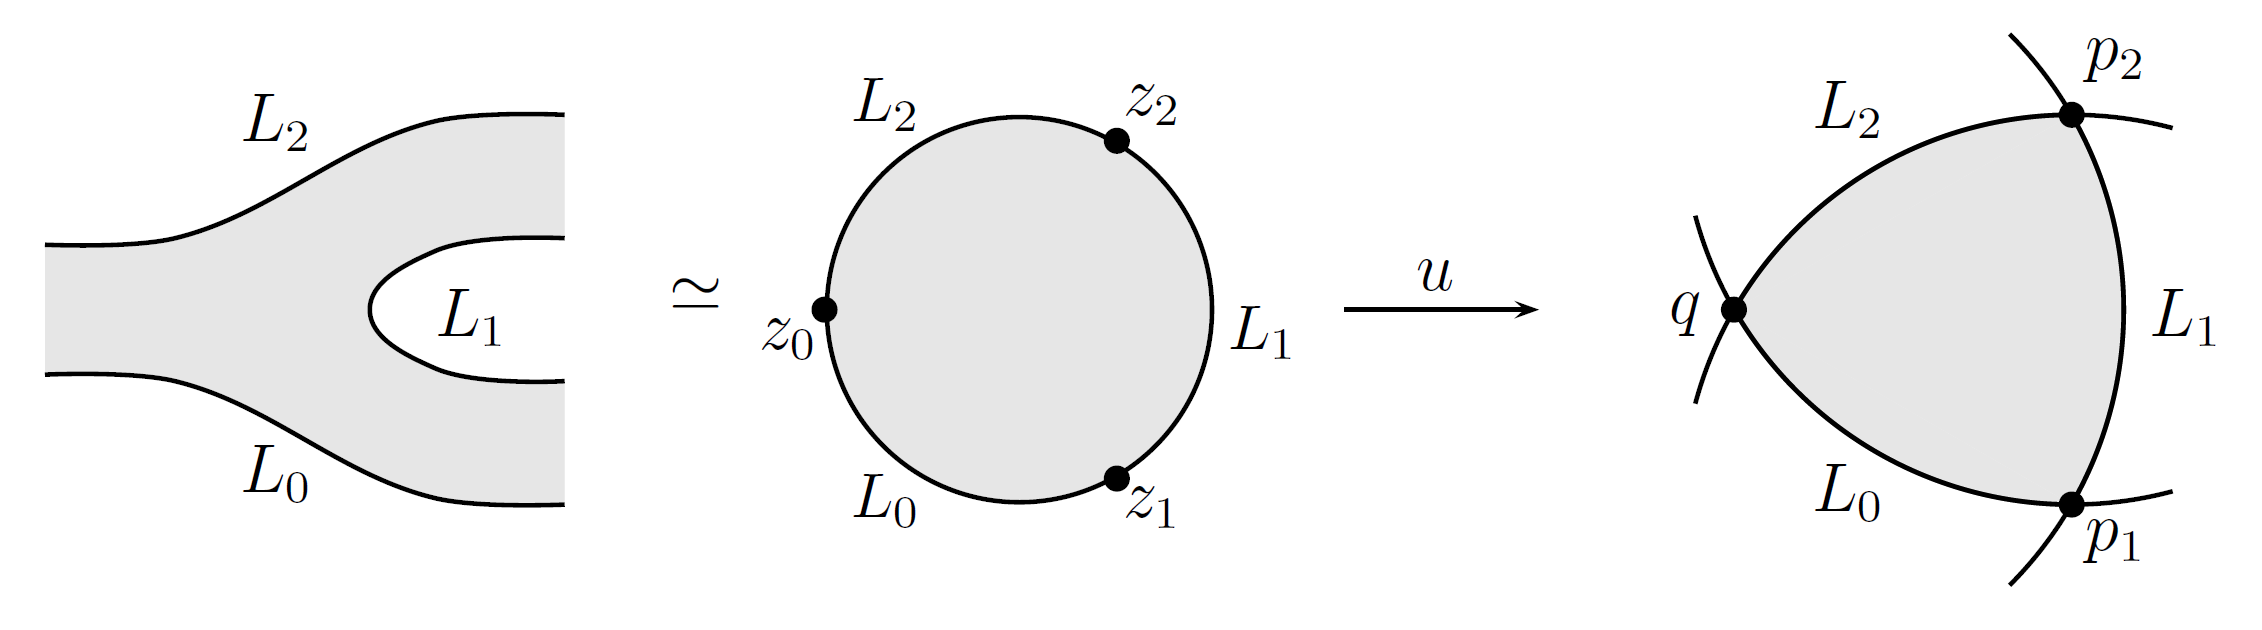
\includegraphics[width=0.9\linewidth]{fig05.png}
  \caption{属于 $\mathcal M(p_1,p_2,q;[u],J)$ 的一条三穿孔 $J$-全纯圆盘 $u$。\hfill（原书 p.85）}
  \label{fig:05}
\end{figure}

\begin{Rem}\label{rem:6.1}
与 (57)--(59) 的相似之处显而易见。事实上，$\mathbb D^2$ 中每个“穿孔” $z_i$
的充分小开邻域都双全纯于 $\mathbb R\times[0,1]\subset\mathbb R^2\cong\mathbb C$，
图~\ref{fig:05} 正强调了这一点：它给出了三穿孔圆盘
$\mathbb D^2\setminus\{z_0,z_1,z_2\}$ 与左端“三端条带”之间的一个双全纯映射。

另一方面，图 2 已经暗示了 $\mathbb D^2\setminus\{\pm1\}$ 与
$\mathbb R\times[0,1]$ 的等同。因此人们可以——而且马上会看到，也应当——
把问题 \eqref{eq:6.78} 理解为第 5 章所讨论内容的“$3$ 次类比”。
\end{Rem}

% [Tutor Note: 【易错】式 (78) 的三段边界弧以 $z_0=-1$、$z_1=e^{-i\pi/3}$、
% $z_2=e^{i\pi/3}$ 为分界点：与 $\mathbb R\times[0,1]$ 的端点 $\pm1$ 不同，
% 这里三段弧的长度都是 $2\pi/3$。计数时三个穿孔点的循环次序固定在
% $\operatorname{Aut}(\mathbb D^2)$ 轨道下才不依赖 $z_j$ 的具体位置。]

注意，与定义 5.12 不同，我们并不要求用 $\mathbb R$ 去除
$\mathcal M(p_1,p_2,q;[u],J)$，因为解空间上不存在整体的自由平移作用。
事实上，自同构群 $\operatorname{Aut}(\mathbb D^2)$ 在带标记边界点的循环有序
三元组上传递作用，所以连 $z_j$ 的选取也无关紧要。于是
$\mathcal M(p_1,p_2,q;[u],J)$ 的维数直接等于 Maslov 指标
$\operatorname{ind}([u])$：

\begin{Lem}\label{lem:6.2}
设 $M^{2n}=(M,\omega,J)$ 是近复辛流形，$2c_1(TM)=0$，而
$L_0,L_1,L_2\subset M$ 是如上拉格朗日子流形，特别地分次且
$[\phi_{L_i}]=0$。则成立
\[
\dim\bigl(\mathcal M(p_1,p_2,q;[u],J)\bigr)
=\operatorname{ind}([u])=\deg(q)-\deg(p_1)-\deg(p_2)\,.
\]
（同样，这也等于由 $D_{\bar\partial_{J,u}}$ 定义的 Fredholm 指标。）
\end{Lem}

\begin{proof}[证明（概要）]
只需改造第 5.4 节给出的 Maslov 指标定义。暂记 $q:=p_0$，沿
$\partial(\operatorname{im}(u))$ 逆时针行进：先把 $u^*TM$ 适当平凡化，
再考虑定义 5.17 所述从 $T_{p_j}L_j$ 到 $T_{p_k}L_j$ 的道路 $l_i$，以及从
$T_{p_i}L_k$ 到 $T_{p_i}L_i$ 的典范短道路 $\lambda_{p_i}$，其中
$(i,j,k)$ 遍取 $(0,1,2)$ 的循环置换；然后研究以 $T_{p_0}L_0$ 为基点的环路
\[
\gamma_u:=l_2*\lambda_{p_1}*l_0*\lambda_{p_2}*l_1*\lambda_{p_0}
\in LGr(n)\,.
\]
定义 5.22 关于生成元次数的论述在此仍成立（并且由我们的假设而有意义）。
于是所断言的等式来自道路拼接下的可加性。
\end{proof}

% [Tutor Note: 【易错】引理 6.2 的指标位移是关键：输出端点 $q$ 贡献
% $+\deg(q)$，两个输入端点各贡献一个负号。这正是 $\mu^2$ 度数为
% $0=2-2$、$\mu^d$ 度数为 $2-d$ 的来源（式 (83)、(84)）。]

% [Tutor Note: 【背景】证明中的环路 $\gamma_u$ 按
% $l_2,\lambda_{p_1},l_0,\lambda_{p_2},l_1,\lambda_{p_0}$ 交错拼接；
% 若把 $(i,j,k)$ 的循环置换写错方向，会得到反向环路，Maslov 指标相差一个
% 符号。原文按逆时针参数化，与第 5 章定义 5.17 的约定一致。]

引理 6.2 的证明还表明，$CF(L_1,L_2)\otimes CF(L_0,L_1)$ 带有由两个 Floer
复形自然诱导的 $\mathbb Z$-分次（特别地
$\deg(p_2\otimes p_1)=\deg(p_2)+\deg(p_1)$）。

\begin{Def}\label{def:6.3}
设 $M=(M,\omega,J)$ 是近复辛流形，$2c_1(TM)=0$，而
$L_0,L_1,L_2\subset M$ 是带通常装饰的拉格朗日子流形，特别地满足
$\langle\omega\rangle\cdot\pi_2(M,L_i)=0$。\emph{Floer 乘积}
$\cdot:CF(L_1,L_2)\otimes CF(L_0,L_1)\to CF(L_0,L_2)$ 是下述映射的
$\Lambda_{\mathbb K}$-线性延拓：
\begin{equation}
p_2\otimes p_1\longmapsto p_2\cdot p_1
:=\sum_{\substack{q\in\mathcal X(L_0,L_2)\\ [u]:\ \operatorname{ind}([u])=0}}
\bigl(\#\mathcal M(p_1,p_2,q;[u],J)\bigr)\,T^{\omega([u])}\,q\,,
\label{eq:6.79}
\end{equation}
其中 $\mathcal M(p_1,p_2,q;[u],J)$ 是 Cauchy--Riemann 问题 \eqref{eq:6.78}
代表 $[u]\in\pi_2(M,L_0\cup L_1\cup L_2)$ 的解构成的模空间。式
\eqref{eq:6.79} 中的求和良定义（论证同定理 5.39 的证明），而引理 6.2
告诉我们 $\cdot$ 是 $0$ 次映射。
\end{Def}

% [Tutor Note: 【易错】式 (79) 的下标条件写作“[u]: ind([u])=0”，
% 它不是对生成元 $q$ 求和时的附加条件，而是对同伦类求和的范围；
% 对一般的 $(p_1,p_2,q)$ 只有有限多个类满足此条件（由能量下界与
% $\langle\omega\rangle\cdot\pi_2(M,L_i)=0$ 保证）。]

下面考察 Floer 乘积相对于 Floer 微分的核心性质：它满足分次 Leibniz 法则。
我们借助其背后的几何论证来微调微扰、时间依赖近复结构与哈密顿量的选取。

\begin{Pro}\label{pro:6.4}
Floer 乘积满足分次 Leibniz 法则
\begin{equation}
\partial(p_2\cdot p_1)=(-1)^{|p_1|}\partial(p_2)\cdot p_1
-p_2\cdot\partial(p_1)\,,
\label{eq:6.80}
\end{equation}
其中 $|p_1|:=\deg(p_1)$，且各 $\partial$ 是定义 5.37 给出的适当 Floer 微分。
因此，上同调上诱导的乘积
$HF(L_1,L_2)\otimes HF(L_0,L_1)\to HF(L_0,L_2)$ 良定义，并且实际上与
所涉及的微扰数据的选取无关（参见其证明）。
\end{Pro}

% [Tutor Note: 【易错】式 (80) 的符号 $(-1)^{|p_1|}$ 只加在
% $\partial(p_2)\cdot p_1$ 一项上；这是 Koszul 符号法则在“微分是
% 分次导子”上的体现。若把 $p_1,p_2$ 的次序或符号放反，会与
% 式 (85) 中 $d=2$ 的 $A_\infty$-关系差一个整体符号。]

\begin{proof}[证明（概要）]
我们定性解释其中的几何想法，并对照定理 5.39 证明中的做法。取图~\ref{fig:05} 中那样的
生成元 $p_1\in\mathcal X(L_0,L_1)$、$p_2\in\mathcal X(L_1,L_2)$、
$q\in\mathcal X(L_0,L_2)$，以及同伦类
$[u]\in\pi_2(M,L_0\cup L_1\cup L_2)$，设 $\operatorname{ind}([u])=1$。
假定横截性成立，则 $\mathcal M(p_1,p_2,q;[u],J)$ 是光滑 $1$ 维流形；由
Gromov 紧致性定理 5.34，它可以紧化为某个
$\overline{\mathcal M}(p_1,p_2,q;[u],J)$，只需补上断裂条带（按假设，
圆盘冒泡与球面冒泡均被排除）。

但现在有三个“条带状”端点可以聚集能量。由 Maslov 指标在条带断裂下的可加性、
圆盘的指标非负（横截性使然），以及非常值条带的指标至少为 $1$，指标分解
$\operatorname{ind}([u])=\operatorname{ind}([u'])+\operatorname{ind}([u''])$
只有三种可能：适当重新命名后，$u'$ 必是某条指标 $1$ 的条带，而 $u''$ 是以
$L_0,L_1,L_2$ 为边界的指标 $0$ 圆盘。\footnote{这与我们按假设排除的圆盘冒泡
不同：后者的边界落在单条子流形上，并且是唯一能导致能量爆破的圆盘。}
说白了，我们只需把伪全纯三角形 $u$ 在一个角上“捏紧”，见图~\ref{fig:06}。具体地说，
图中所示三种构型分别贡献 $\partial(p_2\cdot p_1)$、$p_2\cdot\partial(p_1)$
与 $\partial(p_2)\cdot p_1$ 中 $T^{\omega([u])}q$ 的系数。

\begin{figure}[htbp]
  \centering
  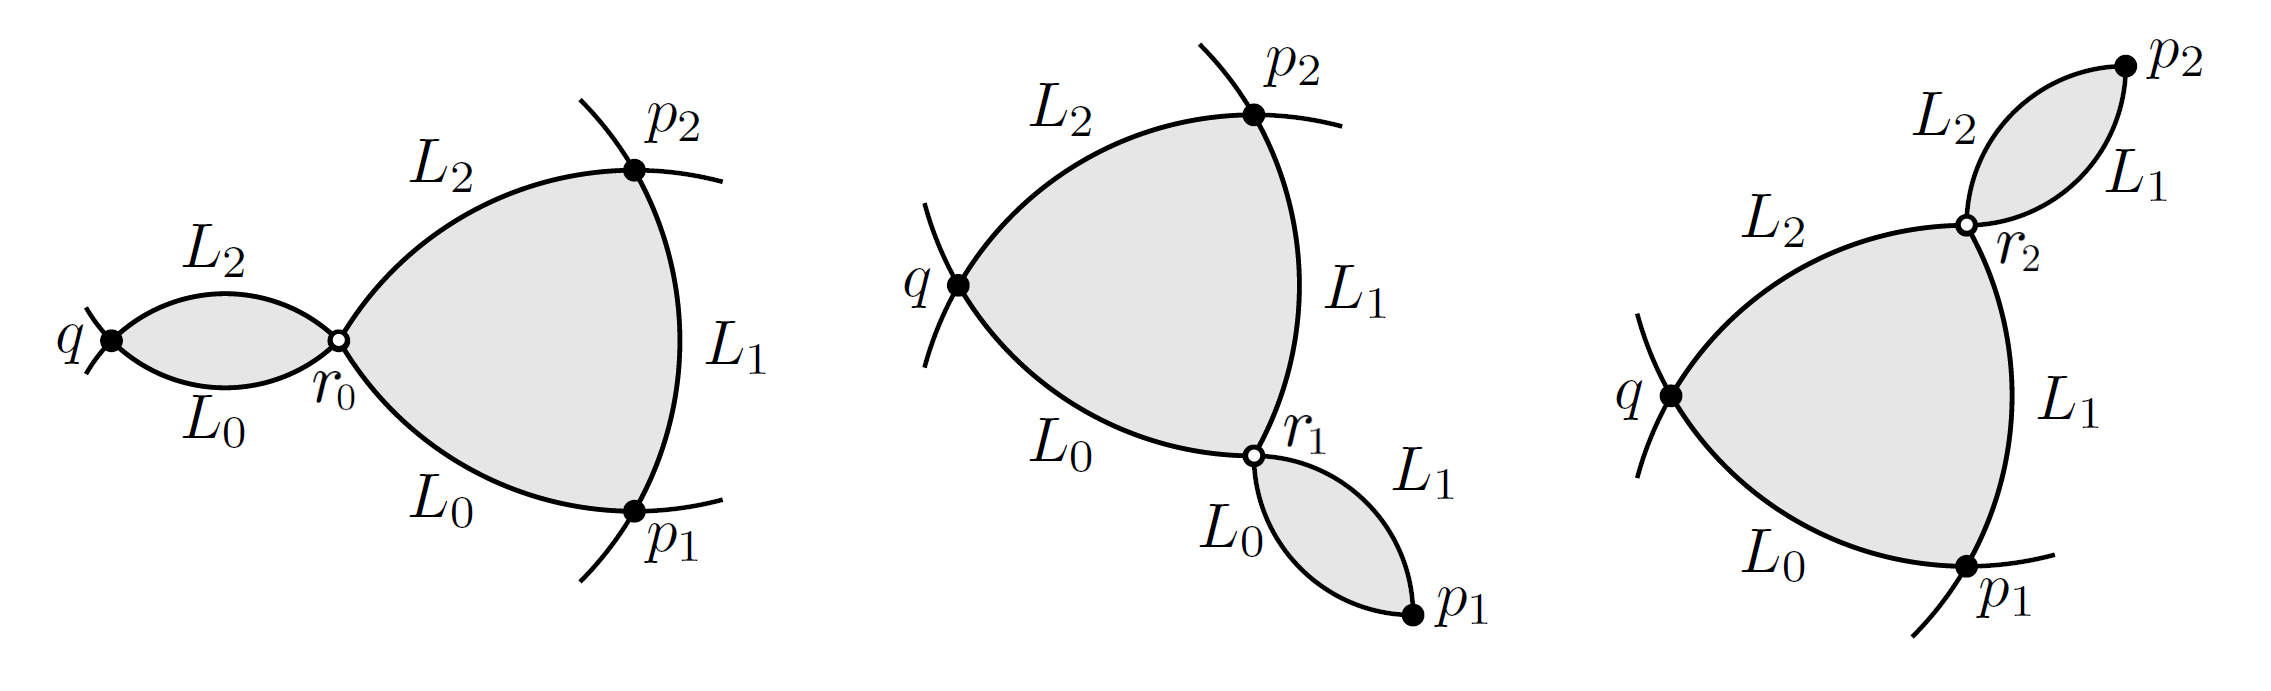
\includegraphics[width=0.9\linewidth]{fig06.png}
  \caption{$\mathcal M(p_1,p_2,q;[u],J)$ 中三穿孔 $J$-全纯圆盘的三类可能极限构型。\hfill（原书 p.87）}
  \label{fig:06}
\end{figure}

这意味着 $\partial\overline{\mathcal M}(p_1,p_2,q;[u],J)$ 包含在形如
$\mathcal M(p_i,r_i;[u'],J)\times\mathcal M(r_i,p_j,p_k;[u''],J)$ 的模空间
乘积的无交并之中，其中 $r_j\in\mathcal X(L_i,L_j)$ 是“捏紧”得到的点
（仍记 $q:=p_0$）。反向包含由另一个粘接定理给出，于是
$\overline{\mathcal M}(p_1,p_2,q;[u],J)$ 确实是紧致 $1$ 维光滑流形，
其边界如上所述（且定向相容）。引理 5.38 告诉我们，后者的（带符号或无符号）
基数为零；对所有同伦类求和并仔细计及次数，即得 Leibniz 法则
\eqref{eq:6.80}。

至于式 \eqref{eq:6.79} 在上同调上诱导出良定义乘积，论证十分容易：若
$\partial(p_1)=\partial(p_2)=0$，则由 \eqref{eq:6.80} 得
$\partial(p_2\cdot p_1)=0$；若再有 $p_1=\partial(p_1')$，则
$p_2\cdot p_1=\partial(p_2\cdot p_1')$。因此闭上链与上边界都被保持，正是
所愿。
\end{proof}

% [Tutor Note: 【含糊】证明中“反向包含由另一个粘接定理给出”省略了
% 全部分析细节：需要先在每条指标 1 的条带与指标 0 的三角形之间建立
% 预粘接（pre-glue），再证明粘接映射是微分同胚。完整论证见
% \cite{Sei08} 第 9 章与 \cite{FOOO09} 第 7–8 章；本译本不补写。]

最后讨论 $L_i\not\pitchfork L_j$ 的一般情形。为达到横截性，我们重新引入
时间依赖的近复结构与哈密顿量：对每个条带状端点取一对
$(J_{ij},H_{ij})\in C^\infty([0,1],\mathcal J(M,\omega))\times
C^\infty([0,1]\times M)$，按所界定的拉格朗日子流形标记
$0\le i<j\le 2$（见图~\ref{fig:05} 左）。注意由注 6.1，这样做是合理的。然而
这一次，这样的数据无法延拓到整个穿孔圆盘：必须选取整体定义的
$J\in C^\infty(\mathbb D^2,\mathcal J(M,\omega))$ 与
$H\in C^\infty(\mathbb D^2\times M)$（即随 $\mathbb D^2$ 光滑变化的族），
使它们在每个 $z_j$ 的固定邻域内与所选的 $(J_{ij},H_{ij})$ 相符。

于是我们只在穿孔附近恢复微扰方程 (66)，那里可以使用全纯局部复坐标
$z=s+it$，$(s,t)\in\mathbb R\times[0,1]$。为看清这一点，取
$\beta\in\Omega^1(\mathbb D^2)$ 使 $\beta|_{S^1}=0$ 且在诸 $z_j$ 附近
$\beta=dt$。微扰 Cauchy--Riemann 方程 (57)，得到
\begin{equation}
(du-X_H\otimes\beta)^{0,1}_J=0\,,
\label{eq:6.81}
\end{equation}
它在三个穿孔附近恰与 Floer 方程重合：
$0=(du-X_H\otimes dt)^{0,1}_J=\partial_s u+J_t(u)(\partial_t u-X_{H_t}(u))$，
其中 $J$ 与 $H$ 仅依赖 $t$。与第 5.5 节所得类似，有
$\mathcal X(L_i,L_j)=L_i\cap(\phi^1_{H_{ij}})^{-1}(L_j)$；上面几段的证明
可原样搬到微扰乘积映射
$\cdot:CF(L_1,L_2;J_{12},H_{12})\otimes CF(L_0,L_1;J_{01},H_{01})
\to CF(L_0,L_2;J_{02},H_{02})$ 上，于是它满足 Leibniz 法则。

% [Tutor Note: 【易错】式 (81) 中 $\beta$ 在 $S^1$ 上为零、在穿孔附近为 $dt$，
% 因此 $(du-X_H\otimes\beta)^{0,1}_J$ 的微扰项只在穿孔附近出现；若取
% $\beta=dt$ 整体定义，则方程不再与 Floer 方程局部相符。另注意
% $(\,\cdot\,)^{0,1}_J$ 是 $J$-反线性部分的投影，$\beta$ 是实 $1$-形式。]

\subsection{高阶复合映射}\label{sec:6.2}

现在考虑涉及 $(d+1)$ 条拉格朗日子流形 $L_0,\dots,L_d\subset M$ 的高阶乘积，
它们带有通常的装饰。

给定 $d+1$ 个生成元 $p_1\in\mathcal X(L_0,L_1)$，
$p_2\in\mathcal X(L_1,L_2)$，……，
$p_d\in\mathcal X(L_{d-1},L_d)$，$q\in\mathcal X(L_d,L_0)$，以及边界穿孔
$z_j=e^{i\pi(1+2j/(d+1))}$、$z_0=-1\in S^1$（$j=1,\dots,d$）；我们要找
$J$-全纯映射 $u:\mathbb D^2\setminus\{z_0,z_1,\dots,z_d\}\to M$，满足微扰
Cauchy--Riemann 方程 \eqref{eq:6.81} 的 $(d+1)$ 次类比，边界条件为
\begin{equation}
\left\{
\begin{aligned}
&u(e^{i\alpha})\in L_0 \quad \text{若}\ \alpha\in\Bigl(\pi,\pi+\tfrac{2\pi}{d+1}\Bigr)
&&\text{且}\ \lim_{z\to z_0}u(z)=q\,,\\[2pt]
&u(e^{i\alpha})\in L_j \quad \text{若}\ \alpha\in\Bigl(\pi+\tfrac{2j\pi}{d+1},\pi+\tfrac{2(j+1)\pi}{d+1}\Bigr)
&&\text{且}\ \lim_{z\to z_j}u(z)=p_j\,,
\end{aligned}
\right.
\label{eq:6.82}
\end{equation}
并且能量有限，$E(u)<\infty$。我们称其为\emph{广义 Cauchy--Riemann 问题}。
代表固定同伦类 $[u]\in\pi_2\bigl(M,\bigcup_{i=0}^d L_i\bigr)$ 的解构成模空间
$\mathcal M(p_1,\dots,p_d,q;[u],J,H)$。情形如图~\ref{fig:07} 所示，该图也说明为何
$J$-全纯解 $u$ 的像 $\operatorname{im}(u)$（进而 $u$ 本身）被称为
\emph{伪全纯多边形}。

这里我们已经选取了适当的、依赖定义域的
$J\in C^\infty(\mathbb D^2,\mathcal J(M,\omega))$ 与
$H\in C^\infty(\mathbb D^2\times M)$，并注意（见下文定义 6.9）如下事实：
与上一节 $d=2$ 的情形不同，此处循环有序元组
$(z_0,z_1,\dots,z_d)\subset S^1$ 有许多选法，区别在于每个穿孔在其弧上的
确切相对位置。

\begin{Def}\label{def:6.5}
设 $\operatorname{Punct}_{d+1}$ 是边界穿孔的一切有序构型
$(z_0,z_1,\dots,z_d)\subset S^1$ 构成的空间（$d\ge 2$），
$\operatorname{Aut}(\mathbb D^2)$ 是 $\mathbb D^2$ 的双全纯群。则
$\mathcal M_{0,d+1}:=\operatorname{Punct}_{d+1}/\operatorname{Aut}(\mathbb D^2)$
是 $\mathbb D^2$ 上\emph{共形结构}的模空间，它是一个可缩的 $(d-2)$ 维
光滑流形。
\end{Def}

\begin{figure}[htbp]
  \centering
  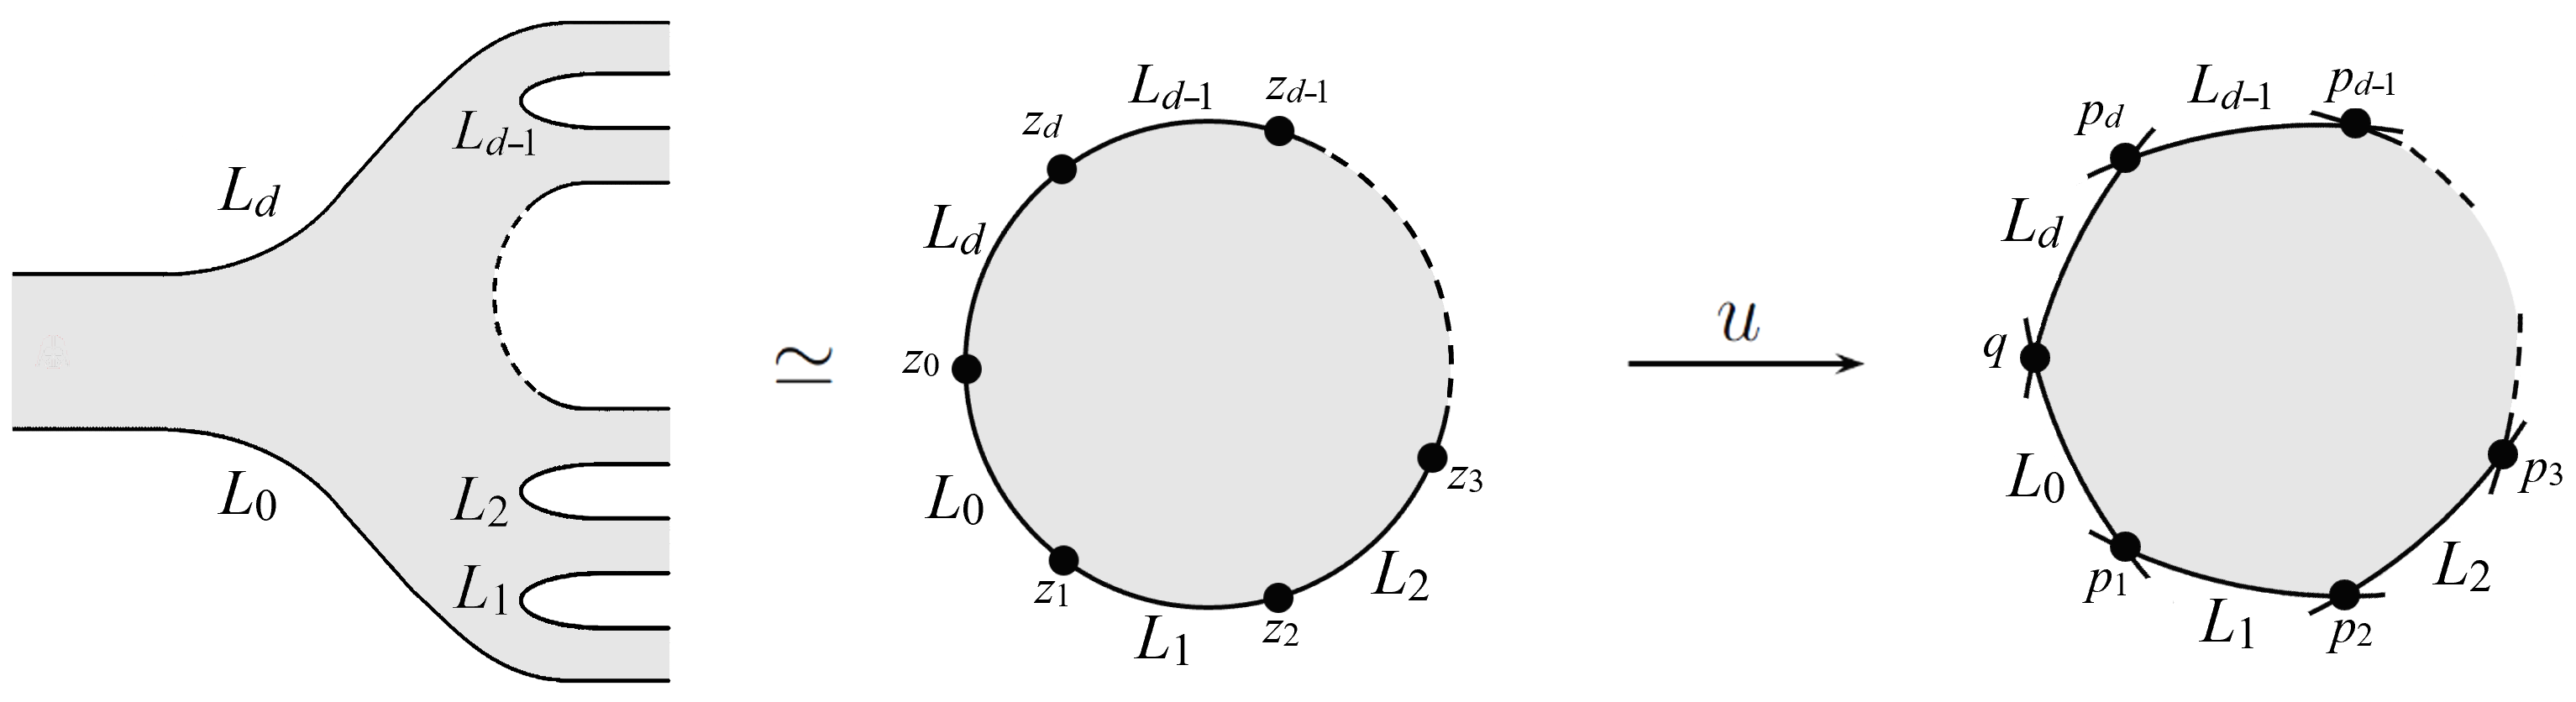
\includegraphics[width=0.9\linewidth]{fig07.png}
  \caption{属于 $\mathcal M(p_1,\dots,p_d,q;[u],J,H)$ 的一条 $(d+1)$-穿孔 $J$-全纯圆盘 $u$。\hfill（原书 p.89）}
  \label{fig:07}
\end{figure}

空间 $\mathcal M_{0,d+1}$ 有自然的紧化，得到 $(d-2)$ 维多胞形
$\overline{\mathcal M}_{0,d+1}$——（同胚地）正是我们在第 1.1 节遇到的
结合面体 $K_d$！其边界 $\partial\overline{\mathcal M}_{0,d+1}$ 参数化
$\mathbb D^2$ 的一切可能退化（\emph{节点退化}），退化为若干子圆盘，每个
至少携带一个穿孔 $z_j$。具体地说，每个 $(d-3)$-骨架分支对应一类（同伦类
意义下的）退化为两个圆盘、每个至少保留两个穿孔；同样，$(d-4)$-骨架可
指派三个圆盘的构型，如此类推。

% [Tutor Note: 【背景】$\mathcal M_{0,d+1}$ 的维数是 $d-2$：$d+1$ 个边界
% 穿孔在 $S^1$ 上共 $d+1$ 个自由度，商去 $\operatorname{Aut}(\mathbb D^2)$
% 的 $3$ 个自由度，得 $d-2$。紧化把它添成结合面体 $K_d$，其面的偏序
% 恰对应括号的插入方式；这正是 $A_\infty$-关系的几何来源。]

\begin{Ex}\label{ex:6.6}
设 $d=3$。我们知道紧化的 $1$ 维多胞形 $\overline{\mathcal M}_{0,4}=K_3$
同胚于 $[0,1]\subset\mathbb R$（见图 1 左下）。构成其 $0$-骨架的两个端点
标记 $\mathbb D^2$ 在固定穿孔 $z_1,z_2,z_3\in S^1$ 时（不失一般性）的两种
可能退化：或者 $z_0\in S^1$ 可沿 $L_0$ 向 $z_1$ “滑动”，最终与它一起落入
对应 $0$ 的退化构型的某个子圆盘中；或者它沿 $L_3$ 向 $z_3$ 滑动，产生
对应 $1$ 的构型（见图~\ref{fig:08}）。
\end{Ex}

\begin{figure}[htbp]
  \centering
  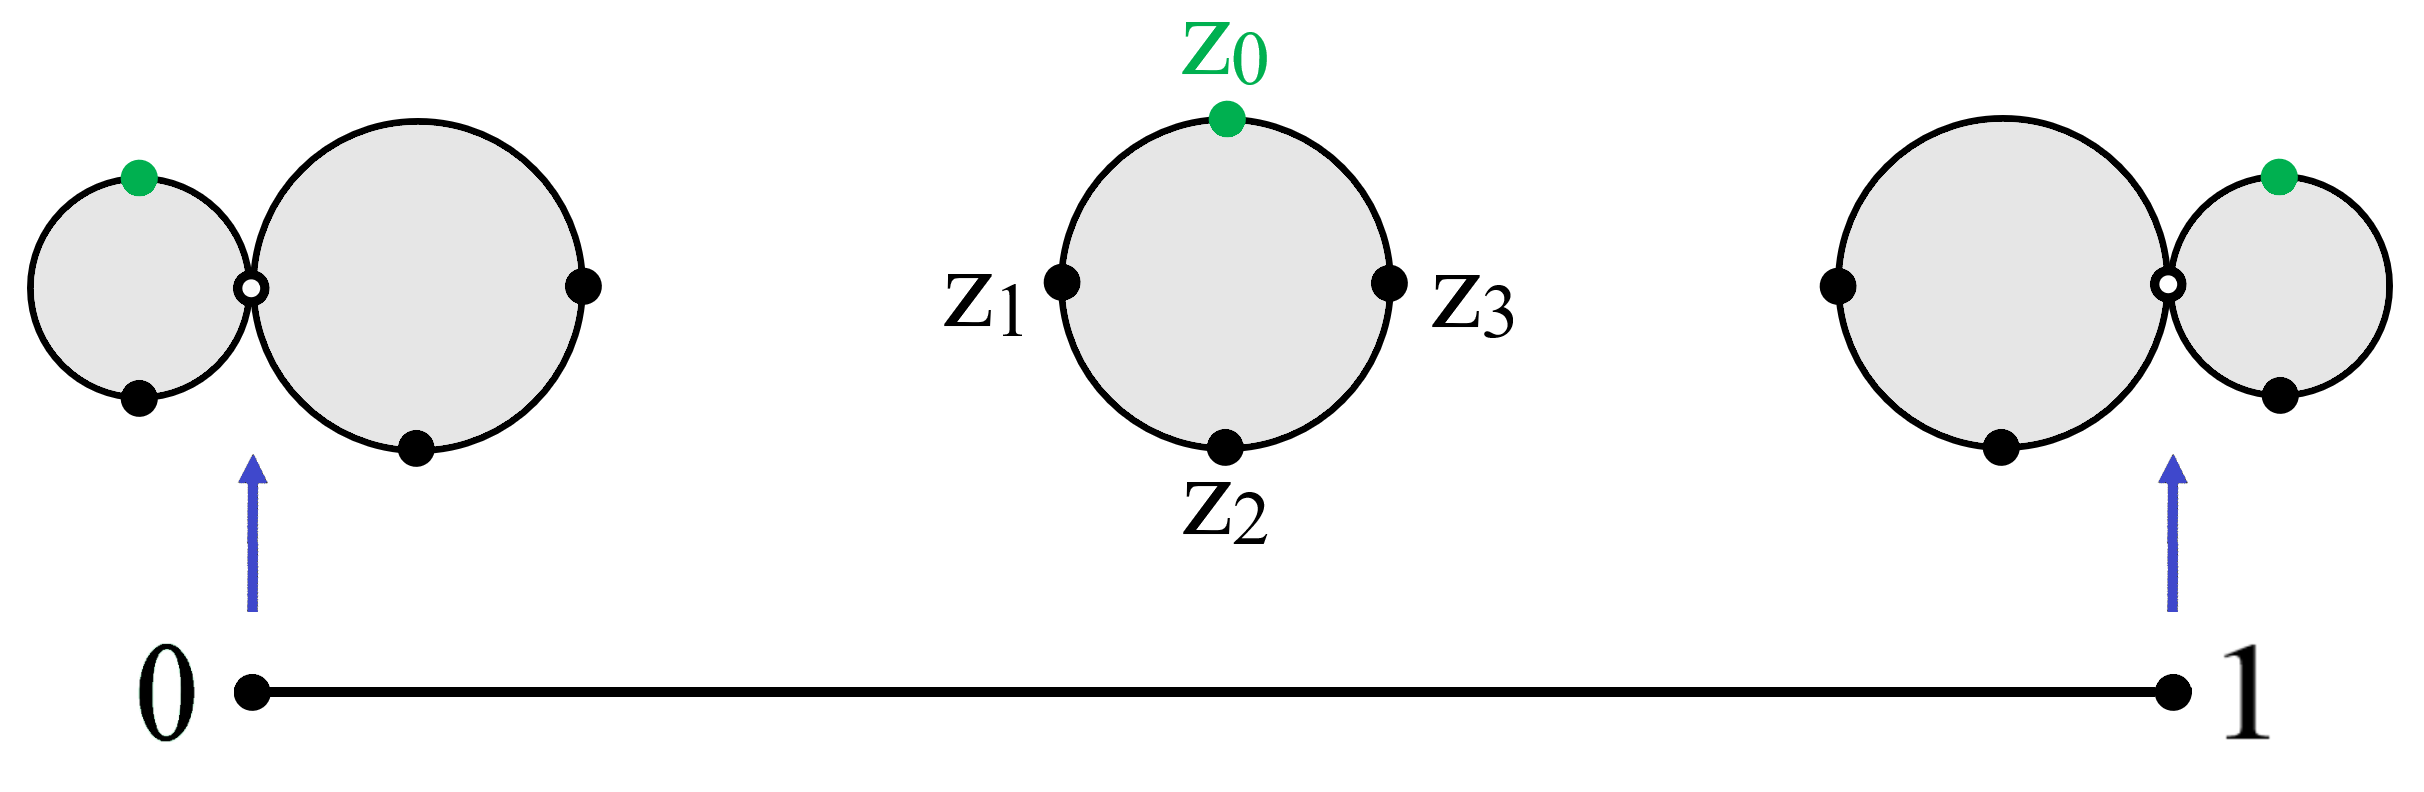
\includegraphics[width=0.8\linewidth]{fig08.png}
  \caption{多胞体 $\overline{\mathcal M}_{0,4}=K_3$ 及其对应的退化极限构型（白点表示新生成的节点）。\hfill（原书 p.89）}
  \label{fig:08}
\end{figure}

换个方式，我们也可固定 $z_0,z_1,z_2$ 而让 $z_3$ 变动。这个“滑动操作”
——由第 1.1 节的同伦 $m_3$ 形式化——会对 Floer 复形上的某些高阶复合映射
作出贡献，下面将予以说明。

\begin{Rem}\label{rem:6.7}
在上一个例子的基础上，可以如下解释 $\mathcal M_{0,d+1}$ 的定义。群
$\operatorname{Aut}(\mathbb D^2)\cong PSL(2,\mathbb R)$ 是 $3$ 维 Lie 群，
其作用至多能唯一固定 $\mathbb D^2$ 的三个边界穿孔（事实上
$\mathcal M_{0,3}=\operatorname{Punct}_3/\operatorname{Aut}(\mathbb D^2)$
是 $0$ 维的，故可忽略，正如紧接注 6.1 之后的讨论所示）。若 $d>2$，
即若处理多于三个穿孔，则这些穿孔可自由地沿映入拉格朗日子流形的弧滑动，
从而在 $\mathcal M_{0,d+1}$ 中产生非平凡的不同类。模去可被固定的三个穿孔，
便知 $\mathcal M_{0,d+1}$ 具有 $(d+1)-3=d-2$ 维光滑流形的结构。

与例 6.6 类似，当两个或更多穿孔撞在一起时，$\mathbb D^2$ 便发生节点退化，
由此产生冒泡效应；该效应消解为若干携带相关点的子圆盘。$\mathcal M_{0,d+1}$
的紧化就是把这类极限构型一并纳入，它们由 $\partial\overline{\mathcal M}_{0,d+1}$
标定。
\end{Rem}

\begin{Ex}\label{ex:6.8}
对 $\overline{\mathcal M}_{0,5}=K_4$ 的直观理解如下。给定五个穿孔
$z_0,z_1,z_2,z_3,z_4\in S^1$，固定一个（相邻的！）三元组，比如
$z_1,z_2,z_3$，而让 $z_0,z_4$ 变动。我们有十种方式让这一对“相撞”。
例如 $z_0$ 可以撞上 $z_1$，我们不妨将其写作 $(z_0*z_1)$。其余组合为
（沿图~\ref{fig:09} 逆时针移动）：
$(z_4*(z_0*z_1))$、$(z_4*z_0*z_1)$、$((z_4*z_0)*z_1)$、
$(z_4*z_0)$、$(z_3*(z_4*z_0))$、$(z_3*z_4*z_0)$、
$((z_3*z_4)*z_0)$、$(z_3*z_4)$ 以及 $(z_0*z_1)(z_3*z_4)$。

括号至关重要，因为它们规定了碰撞的次序！事实上，$(z_4*z_0*z_1)$ 对应
退化为两个子圆盘、其中一个携带 $z_0,z_1,z_4$ 的节点退化；而
$(z_4*(z_0*z_1))$ 编码三个圆盘的构型，其中间的圆盘携带 $z_4$，末端的
圆盘收集 $z_0$ 与 $z_1$。显然，所列组合中有五个标定五边形 $K_4$ 的边
（即其 $1$-骨架），另外五个标定其顶点（$0$-骨架）。
\end{Ex}

\begin{figure}[htbp]
  \centering
  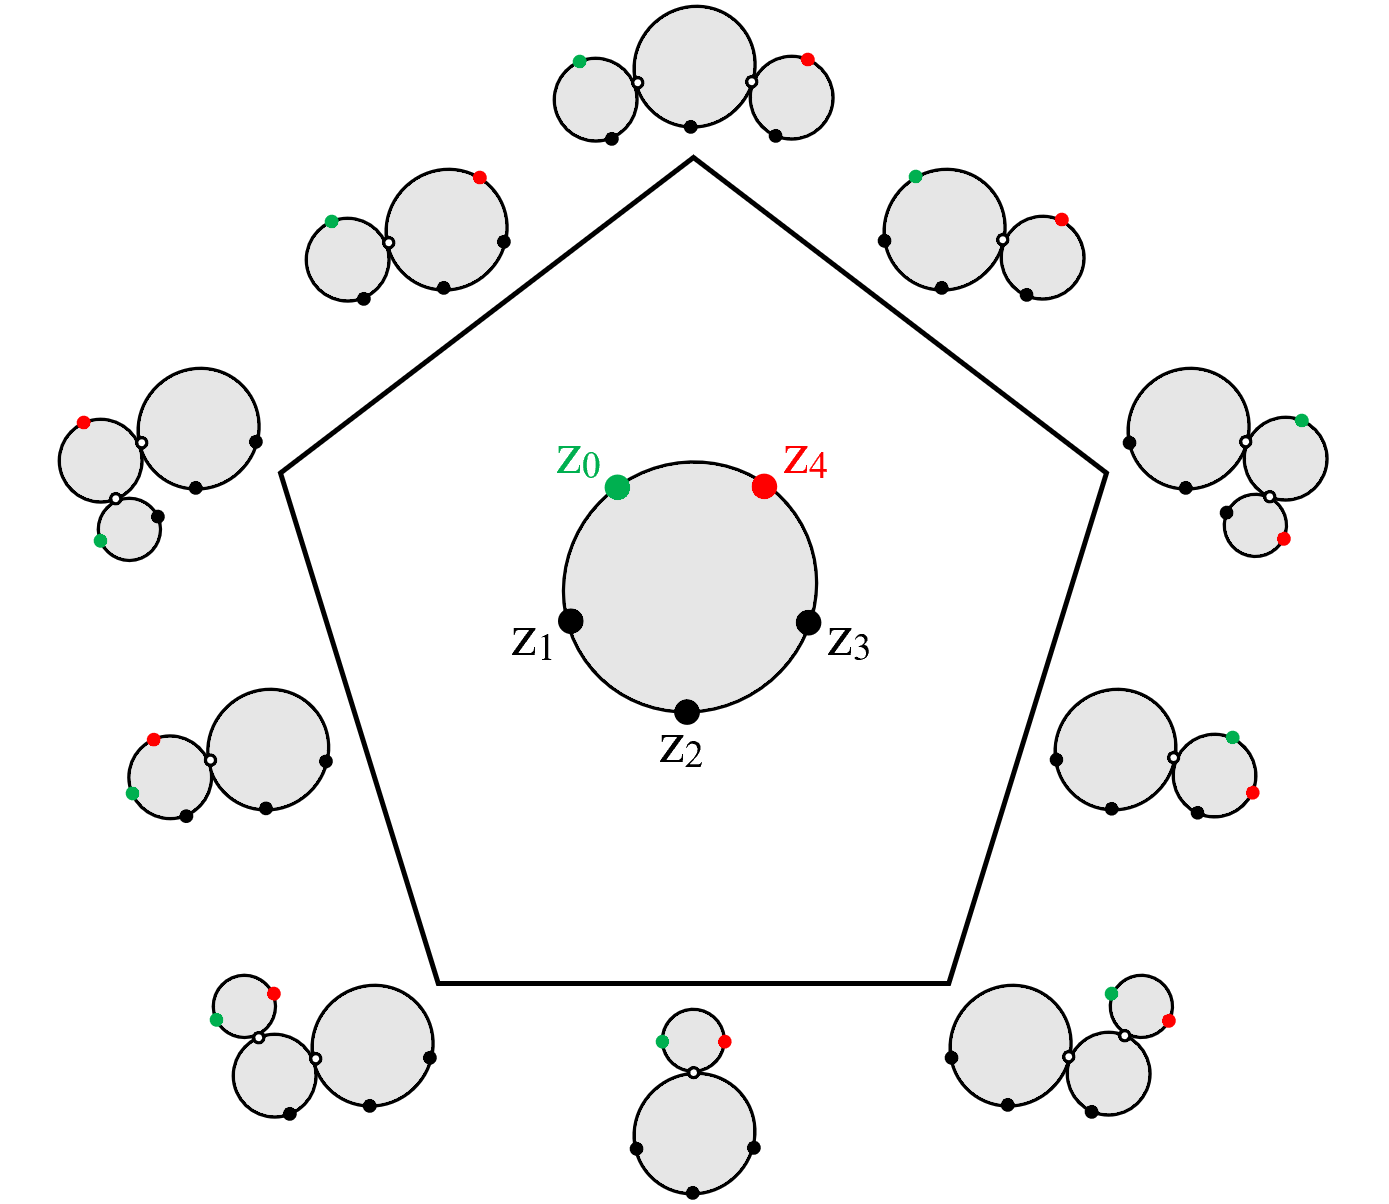
\includegraphics[width=0.55\linewidth]{fig09.png}
  \caption{多胞体 $\overline{\mathcal M}_{0,5}=K_4$ 及其对应的退化极限构型（白点表示新生成的节点）。\hfill（原书 p.90）}
  \label{fig:09}
\end{figure}

我们有意让变量保持循环次序，以凸显另一种解释：$K_d$ 的
$(d-r)$-骨架分支对应于在字符串 $z_0z_1\cdots z_{d-1}z_d$ 中适当插入
$r-2$ 对括号。例如
$(z_4*(z_0*z_1))\equiv(z_0z_1))z_2z_3(z_4$。这使得研究高维结合面体大大
简化。读者不妨考察 $K_5$（图 1 中最右侧者），其九个面、二十一条边与
十四个顶点分别参数化退化为两个、三个与四个子圆盘的可能节点退化。

% [Tutor Note: 【勘误】“$(z_4*(z_0*z_1))\equiv(z_0z_1))z_2z_3(z_4$”这一
% 括号串在原书中括号不平衡（左括号与右括号数目不等）。原文如此印，
% 疑为“$(z_0z_1))z_2z_3(z_4$”想表达的是把 $z_4$ 与 $(z_0*z_1)$ 分别
% 归入两个子圆盘的括号插入；译文照印，读者理解其意即可，勿据此做符号推导。]

最后说明在 $d+1$ 条拉格朗日子流形的一般情形下如何选取相容的微扰数据。
其存在性的证明见 \cite{Sei08} 引理 9.5。

\begin{Def}\label{def:6.9}
给定共形结构 $(z_0,z_1,\dots,z_d)\in\mathcal M_{0,d+1}$，考虑相应的、
形如 \eqref{eq:6.81}、带边界条件 \eqref{eq:6.82} 与有限能量约束的广义
Cauchy--Riemann 问题。再考虑确定 $CF(L_i,L_j)$ 的时间依赖
$(J_{ij},H_{ij})\in C^\infty([0,1],\mathcal J(M,\omega))\times
C^\infty([0,1]\times M)$，对每个条带状端点（即定义在 $p_j$ 与 $q$ 的固定
邻域上、可用全纯局部坐标之处）按所界定的拉格朗日子流形标记
$0\le i<j\le d$。为达到横截性，我们选取
$J\in C^\infty(\mathbb D^2,\mathcal J(M,\omega))$ 与
$H\in C^\infty(\mathbb D^2\times M)$，使得：
\begin{itemize}
  \item $(J,H)$ 在相应的条带状端点上与每个 $(J_{ij},H_{ij})$ 相符；
  \item 按定义 6.5 的方式使 $\mathbb D^2$ 节点退化时，$J$ 与 $H$ 在节点
  周围的（条带状）区域中平移不变，并且确实与那里的局部哈密顿量及近复结构
  重合。
\end{itemize}
我们称这样的对 $(J,H)$ 为 \emph{Floer 数据}；由构造，它依赖于
$(z_0,z_1,\dots,z_d)$ 以及所有 $J_{ij}$ 与 $H_{ij}$。于是由此产生的 Floer
上同调称为“无障碍的（unobstructed）”。
\end{Def}

% [Tutor Note: 【含糊】“Floer 数据”的相容性只是逐条列出的要求，原文并未
% 构造它；存在性完全依赖 \cite{Sei08} 引理 9.5 的归纳构造（逐次在
% 结合面体的骨架上延拓）。所谓“unobstructed”指 $\mu^0=0$、从而
% $A_\infty$-关系不被圆盘冒泡破坏，而非指模空间自动正则。]

$\mathcal M_{0,d+1}$ 的介入还意味着必须相应改造引理 6.2 及其证明。

\begin{Lem}\label{lem:6.10}
固定共形结构 $(z_0,z_1,\dots,z_d)\in\mathcal M_{0,d+1}$ 及如上述相容的
Floer 数据 $(J,H)\in C^\infty(\mathbb D^2,\mathcal J(M,\omega))\times
C^\infty(\mathbb D^2\times M)$。考虑相应的广义 Cauchy--Riemann 问题，它对
每个解 $[u]\in\pi_2\bigl(M,\bigcup_{i=0}^d L_i\bigr)$ 给出模空间
$\mathcal M(p_1,\dots,p_d,q;[u],J,H)$。则
\begin{equation}
\begin{aligned}
\dim\bigl(\mathcal M(p_1,\dots,p_d,q;[u],J,H)\bigr)
&=\dim(\mathcal M_{0,d+1})+\operatorname{ind}([u])\\
&=d-2+\deg(q)-\sum_{i=1}^{d}\deg(p_i)\,,
\end{aligned}
\label{eq:6.83}
\end{equation}
其中 $\dim(\mathcal M_{0,d+1})$ 计入 $(z_0,z_1,\dots,z_d)$ 的可能形变。
\end{Lem}

\begin{Def}\label{def:6.11}
设 $(M,\omega,J)$ 是近复辛流形，$2c_1(TM)=0$，而 $L_0,\dots,L_d\subset M$
是带通常装饰的拉格朗日子流形，特别地满足
$\langle\omega\rangle\cdot\pi_2(M,L_i)=0$。选取 Floer 数据
$(J,H)\in C^\infty(\mathbb D^2,\mathcal J(M,\omega))\times
C^\infty(\mathbb D^2\times M)$ 以达到横截性。第 $d$ 个 \emph{Floer 复合映射}
$\mu^d:CF(L_{d-1},L_d)\otimes\cdots\otimes CF(L_0,L_1)\to CF(L_0,L_d)$
是下述映射的 $\Lambda_{\mathbb K}$-线性延拓：
\begin{equation}
\mu^d(p_d,\dots,p_1):=\sum_{\substack{q\in\mathcal X(L_0,L_d)\\
[u]:\ \operatorname{ind}([u])=2-d}}
\bigl(\#\mathcal M(p_1,\dots,p_d,q;[u],J,H)\bigr)\,
T^{\omega([u])}\,q\,,
\label{eq:6.84}
\end{equation}
\end{Def}

其中 $\mathcal M(p_1,\dots,p_d,q;[u],J,H)$ 是广义 Cauchy--Riemann 问题
\eqref{eq:6.81} 代表 $[u]\in\pi_2\bigl(M,\bigcup_{i=0}^d L_i\bigr)$ 的解
构成的模空间。按通常论证，该求和良定义；并且注意引理 6.10 使 $\mu^d$
成为次数 $2-d$ 的分次映射。

特别地，$\mu^1=\partial_{J,H}$ 是（$1$ 次的）Floer 微分 (74)，而
$\mu^2=\cdot$ 是（$0$ 次的）Floer 乘积 \eqref{eq:6.79}。

% [Tutor Note: 【易错】式 (84) 的指标条件 $\operatorname{ind}([u])=2-d$
% 必须与式 (83) 联读：由 $\dim(\mathcal M)=d-2+\operatorname{ind}([u])$
% 及 $\operatorname{ind}([u])=2-d$ 知所计数的模空间是 $0$ 维的；而式 (83)
% 的另一个表达式给出 $\deg(q)-\sum_i\deg(p_i)=2-d$。换言之，指标条件
% $\operatorname{ind}=2-d$ 正是“$\mu^d$ 的度数为 $2-d$”的另一种说法。
% 这也是 $\mu^1$ 为 $1$ 次、$\mu^2$ 为 $0$ 次的原因。]

\begin{Pro}\label{pro:6.12}
Floer 复合映射 $\mu^d$ 满足 $A_\infty$-结合关系 (6)：
\begin{equation}
\sum_{\substack{1\le m\le d\\ 0\le n\le d-m}}(-1)^{\dagger_n}\,
\mu^{d-m+1}\bigl(p_d,\dots,p_{n+m+1},
\mu^m(p_{n+m},\dots,p_{n+1}),p_n,\dots,p_1\bigr)=0\,,
\label{eq:6.85}
\end{equation}
在 $CF(L_0,L_d)$ 中成立，其中 $p_i\in CF(L_{i-1},L_i)$，且
$\dagger_n:=\bigl(\sum_{i=1}^{n}|p_i|\bigr)-n$。\footnote{鉴于式
\eqref{eq:6.85}，我们的确用 $|p_i|$ 取代了 $\deg(p_i)$。}
\end{Pro}

对 $d=1,2$，前两个这样的方程即 $\partial(\partial(p_1))=0$ 与
$\partial(p_2\cdot p_1)=(-1)^{|p_1|}\partial(p_2)\cdot p_1
-p_2\cdot\partial(p_1)$（分次 Leibniz 法则 \eqref{eq:6.80}）。特别地，
$d=3$ 的情形说明 Floer 乘积 $\mu^2$ 在 $\mu^3$ 给出的同伦意义下结合，
因而在上同调上结合。

% [Tutor Note: 【易错】式 (85) 的符号 $(-1)^{\dagger_n}$ 只依赖前 $n$ 个
% 输入 $p_1,\dots,p_n$ 的次数，且指数里减的是 $n$ 而非 $n-1$——这来自
% 悬挂 $s$ 的次数平移约定（见第 2 章式 (6)）。若漏掉 $-\,n$，则
% $d=2$ 时无法退化为式 (80) 的符号 $(-1)^{|p_1|}$。]

% [Tutor Note: 【易错】原书用一个脚注说明：从式 (85) 起改用 $|p_i|$ 代替
% $\deg(p_i)$。两种记号指同一个次数，并非两种分次；译文在式 (83) 中保留
% $\deg$、在式 (85) 及以后用 $|\cdot|$，与原书一致。]

\begin{proof}[证明（概要）]
$d=1,2$ 的情形已分别由定理 5.39 与命题 6.4 处理。后者的证明也顺带说明了
$\mu^2$ 在上同调上的结合性。

为证明一般恒等式 \eqref{eq:6.85}，我们按“通常”步骤进行：在定义 6.11 的
框架下，考察满足 $\operatorname{ind}([u])=3-d$ 的类
$[u]\in\pi_2\bigl(M,\bigcup_{i=0}^d L_i\bigr)$ 及其模空间
$\mathcal M(p_1,\dots,p_d,q;[u],J,H)$；由式 \eqref{eq:6.83}、横截性与
命题 5.34，它们是 $1$ 维光滑流形，紧化为某个
$\overline{\mathcal M}(p_1,\dots,p_d,q;[u],J,H)$，其边界点或者对应
\begin{itemize}
  \item 在 $d+1$ 个生成元之一处断裂的指标 $1$ 的 $J$-全纯条带，它们随后
  与伪全纯多边形分离（如图~\ref{fig:06}），或者
  \item 由 $\overline{\mathcal M}_{0,d+1}$ 的 $(d-3)$-骨架描述的
  $\mathbb D^2$ 节点退化，即两个圆盘、每个至少携带两个穿孔（如图~\ref{fig:08}）。
\end{itemize}
前者由生成元之一处的能量聚集引起，产生 \eqref{eq:6.85} 中所有含 $\mu^1$
的项；后者起源于穿孔互相“撞上”（如注 6.7 所解释），贡献
\eqref{eq:6.85} 中其余全部被加项。所需等式仍由下述论证得到：空间
$\overline{\mathcal M}(p_1,\dots,p_d,q;[u],J,H)$ 是紧致 $1$ 维流形，
其边界定向相容，故带符号基数必为零；最后对所有同伦类求和。\footnote{关于
从 Morse--Bott Floer 理论角度出发的略有不同的处理，可参阅 \cite{Fuk02a}
第 3 节。}

下面讨论 $d=3$ 的情形。$\overline{\mathcal M}(p_1,p_2,p_3,q;[u],J,H)$ 中
第一类边界点是自指标 $-1$ 的伪全纯方形在其四个穿孔之一处断裂出的指标 $1$
条带；它们对应
$\partial(\mu^3(p_3,p_2,p_1))$、$\mu^3(p_3,p_2,\partial p_1)$、
$\mu^3(p_3,\partial p_2,p_1)$ 与 $\mu^3(\partial p_3,p_2,p_1)$ 这几项。
第二类边界点则对应例 6.6 所述两种节点构型，即两个二穿孔的指标 $0$ 圆盘；
它们给出 $p_3\cdot(p_2\cdot p_1)$ 与 $(p_3\cdot p_2)\cdot p_1$。系数由
生成元的次数决定，于是相应的 $A_\infty$-恒等式确实成立。
\end{proof}

\subsection{Fukaya 范畴的 $A_\infty$ 结构}\label{sec:6.3}

我们终于可以开始收获第一部分的果实了。

\begin{Def}\label{def:6.13}
设 $M=(M,\omega)$ 是满足 $2c_1(TM)=0$ 的辛流形。其（紧致）\emph{Fukaya 范畴}
$\mathcal F(M)$ 是由以下数据刻画的 $A_\infty$-范畴：
\begin{itemize}
  \item 对象集 $\operatorname{obj}(\mathcal F(M))$，由 $M$ 的紧致、可定向、
  自旋、分次的拉格朗日子流形 $L_i\subset M$ 组成，其 Maslov 类消没：
  $\mu_{L_i}\equiv[\phi_{L_i}]=0\in H^1(L;\mathbb Z)$，并满足无冒泡条件
  $\langle\omega\rangle\cdot\pi_2(M,L_i)=0$；连同隐含选取的分次提升
  $\tilde\phi_{L_i}:L_i\to\mathbb R$ 与自旋结构。
  \item 微扰数据
  $(J_{L,L'},H_{L,L'})\in C^\infty([0,1],\mathcal J(M,\omega))\times
  C^\infty([0,1]\times M)$，对每一对 $(L,L')\subset\operatorname{obj}(\mathcal F(M))$；
  以及定义 6.9 中那样的 Floer 数据
  $(J,H)\in C^\infty(\mathbb D^2,\mathcal J(M,\omega))\times
  C^\infty(\mathbb D^2\times M)$，对每个元组
  $(L_0,\dots,L_d)\subset\operatorname{obj}(\mathcal F(M))$；于是它们在解
  相应广义 Cauchy--Riemann 问题 \eqref{eq:6.82} 的 $J$-全纯曲线的条带状
  区域中，与所有 $(J_{L_i,L_j},H_{L_i,L_j})$ 相容。
  \item 对任意两条 $L_0,L_1\in\operatorname{obj}(\mathcal F(M))$（可以相同），
  $\mathbb Z$-分次自由 $\Lambda_{\mathbb K}$-模
  \begin{equation}
  \hom_{\mathcal F(M)}(L_0,L_1):=CF(L_0,L_1;H_{L_0,L_1})\,,
  \label{eq:6.86}
  \end{equation}
  它来自 (56) 经 $H_{L_0,L_1}$ 所作的哈密顿微扰。
  \item （多）线性 $\mathbb Z$-分次复合映射
  $\mu^d_{\mathcal F(M)}:=\mu^d$ 如 \eqref{eq:6.84}，对每个 $d\ge 1$ 与
  $L_0,\dots,L_d\in\operatorname{obj}(\mathcal F(M))$（于是由命题 6.12 满足
  $A_\infty$-结合关系）。
\end{itemize}
\end{Def}

\begin{Rem}\label{rem:6.14}
\begin{itemize}
  \item 我们已经暗示过，Fukaya 范畴的定义有很多种，取决于对 $M$ 及其
  拉格朗日子流形所作的确切假设。例如，去掉 $2c_1(TM)=0$ 以及对每条
  拉格朗日子流形要求 $[\phi_{L_i}]=0$ 这两个条件，会把 $\mathbb Z$-分次
  降为 $\mathbb Z_2$-分次；再取 $\operatorname{char}(\mathbb K)=2$，便可
  忽略自旋结构。最值得注意的是，wrapped Fukaya 范畴只考虑正合流形，
  建立在第 5.8 节所见内容之上；我们将在下文第 6.5 节简要讨论这一变体。
  Fukaya 范畴的相对版本与投影版本也在 \cite{Sei13} 第 8 节中讨论。
  \item 我们甚至可以对微扰数据作各种改动；然而由此得到的所有
  $A_\infty$-范畴都拟同构（在定义 2.8 的意义下）。这意味着，在同构意义下
  （更准确地说，在拟同构意义下），$\mathcal F(M)$ 是 $M$ 的“辛不变量”
  （详见 \cite{Sei08} 第 10 章）。
  \item 反过来，若去掉无冒泡条件
  $\langle\omega\rangle\cdot\pi_2(M,L_i)=0$，并把定义改写为 Morse--Bott
  Floer 理论的语言，最终会得到\emph{弯曲 $A_\infty$-范畴}的概念：此时
  圆盘冒泡由 $0$ 次复合映射 $\mu^0:L_i\subset M\mapsto\mu^0_{L_i}\in
  CF(L_i,L_i)$ 的像来编码，而 $\mu^0$ 满足 $A_\infty$-结合关系（更多细节
  见 \cite{Aur13} 注 2.11 与 \cite{Fuk02a} 第 3 节）。在这种情形下，
  人们把对象集限制为其 $\mu^0_L$ 是 c-单位元 $e_L$（见下文式
  \eqref{eq:6.87}）之倍数的那些对象；在镜像对称中，这对应所谓的
  “超势”或“中心荷”。
  \item 在低维情形，Fukaya 范畴的存在性与良定义性可能由拓扑约束保证。
  例如，任何满足 $2c_1(TM)=0$ 的 $4$ 维辛流形 $M^4$（如经典
  Calabi--Yau 流形）都不出现冒泡现象（见 \cite{AS09} 引理 3.3），因此其
  相伴的 Fukaya 范畴良定义（尽管其对象——消没 Maslov 类的拉格朗日曲面
  $L^2\subset M$——在哈密顿同痕下的不变性并非先验可得；参看 \cite{AS09}
  引理 3.4）。
\end{itemize}
\end{Rem}

\begin{Def}\label{def:6.15}
设 $M$ 是满足 $2c_1(TM)=0$ 的辛流形，$\mathcal F(M)$ 是其 Fukaya 范畴。
诱导的上同调范畴 $H(\mathcal F(M))$（如定义 2.6 所述）称为
\emph{Donaldson--Fukaya 范畴}或\emph{量子范畴}。具体地说，其对象仍是
拉格朗日子流形，Hom 集是由 Floer 微分诱导的全 Floer 上同调环 (76)。

子范畴 $H^0(\mathcal F(M))\subset H(\mathcal F(M))$ 只考虑每个态射空间的
零次上同调，$\hom_{H^0(\mathcal F(M))}(L_0,L_1):=HF^0(L_0,L_1)$。

注意，由于哈密顿同痕的拉格朗日子流形 $L_1,L_1'\subset M$ 对任意
$L_0\subset M$ 诱导同构
$\hom_{H(\mathcal F(M))}(L_0,L_1)=HF(L_0,L_1)\cong HF(L_0,L_1')
=\hom_{H(\mathcal F(M))}(L_0,L_1')$（参看定义 5.5 与注 5.25），令
$L_0:=L_1$ 便证明它们在 $H(\mathcal F(M))$ 中作为对象同构。这就勾销了
我们在第 5.2 节所加的唯一限制。
\end{Def}

% [Tutor Note: 【易错】$H(\mathcal F(M))$ 的 Hom 集是\emph{全} Floer 上同调
% $HF^\bullet$，而 $H^0$ 只取 $\bullet=0$ 的部分；两者不是同一个范畴。
% 文中“$H(\mathcal F(M))$ 是真正的范畴”依赖引理 6.16 的 c-单位元，
% 而非严格单位元。]

既然 Fukaya 范畴已经就绪，我们自然会关心它作为 $A_\infty$-范畴的幺性。
下面几点观察可参阅 \cite{AS09} 第 3 节。

\begin{Lem}\label{lem:6.16}
对任意 Fukaya 范畴 $\mathcal F(M)$，每条拉格朗日子流形
$L\in\operatorname{obj}(\mathcal F(M))$ 都有上同调单位元
$e_L\in\hom^0_{\mathcal F(M)}(L,L)$，即一个 $0$ 次闭上链（于是
$\mu^1_{\mathcal F(M)}(e_L)=0$），使得在 Donaldson--Fukaya 范畴中
$\langle e_L\rangle=\mathrm{id}_L\in HF(L,L)$。因此 $H(\mathcal F(M))$
是真正的范畴。
\end{Lem}

\begin{proof}[证明（概要）]
回忆
\[
CF^0(L,L)=\bigoplus_{p\in\mathcal X(L,L):\ |p|=0}\Lambda_{\mathbb K}\cdot p\,,
\]
其中 $\mathcal X(L,L)=L\cap(\phi^1_H)^{-1}(L)$ 是 $L$ 与它经适当哈密顿函数
$H\in C^\infty(M\times[0,1])$ 微扰后的副本的横截相交。在所有这样的微扰
$0$ 次生成元 $p$ 中，上同调单位元 $e_L$ 由 Cauchy--Riemann 问题 (66) 的
下述 $1$ 次（即 $d=0$）类比得到：取 $L_0=L_1:=L$，并从一个边界穿孔的
$\mathbb D^2$ 出发（它映为 $e_L$）。所求闭上链为
\begin{equation}
e_L:=\sum_{\substack{q\in\mathcal X(L,L)\\ |q|=0}}
\bigl(\#\mathcal M(q;[u],J,H)\bigr)\,T^{\omega([u])}\,q\,.
\label{eq:6.87}
\end{equation}
借助命题 5.43 可以证明，它确实代表 $HF(L,L)\cong H(L;\Lambda_{\mathbb K})$
中的恒等态射。精确的证明涉及 TQFT 的粘接论证——远远超出本书范围。
\end{proof}

% [Tutor Note: 【含糊】$e_L$ 的“显式公式” (87) 只是一个计数表达式；
% 证明它是单位元需要把带一个边界穿孔的圆盘与条带粘接（TQFT 粘接），
% 原文明确说超出范围。注意 $\mu^0$（圆盘冒泡）在此被无冒泡条件排除，
% 故该式和有限且不含 $\mu^0$ 的项。]

\begin{Lem}\label{lem:6.17}
定义 $\mathcal F(M)$ 的微扰数据可以选得使任意拉格朗日子流形
$L\subset M$ 的上同调单位元 $e_L\in\hom^0_{\mathcal F(M)}(L,L)$ 满足
$\mu^2_{\mathcal F(M)}(e_L,e_L)=e_L$，且当 $d>2$ 时
$\mu^d_{\mathcal F(M)}(e_L,\dots,e_L)=0$。
\end{Lem}

\begin{proof}[证明（概要）]
考虑我们在命题 5.43 的证明中用过的 Morse 函数 $f\in C^\infty(L)$，得到
$HF(L,L)\cong HM(f;\Lambda_{\mathbb K})$。Morse 同调同构于奇异同调，而
在胞腔复形（如光滑流形）的情形，后者又同构于胞腔同调（见 \cite{Hat09}
定理 2.35）。由于 $L^n\subset M^{2n}$ 是 $n$ 维的，$CF(L,L)$
集中在 $0$ 到 $n$ 次之间。于是，由于
$\mu^d_{\mathcal F(M)}(e_L,\dots,e_L)\in CF^{2-d}(L,L)$（$\mu^d$
的度数为 $2-d$），$d>2$ 迫使它为零。

为证 $\mu^2_{\mathcal F(M)}(e_L,e_L)=e_L$，只需取 $f$ 在 $L$ 的每个连通
分支上有唯一最大值与最小值。
\end{proof}

% [Tutor Note: 【易错】关键的一步是次数限制：$L$ 是 $n$ 维的，Morse 指标
% 取值于 $[0,n]$，故 $CF(L,L)$ 集中在 $0$ 到 $n$ 次，而
% $\mu^d(e_L,\dots,e_L)\in CF^{2-d}(L,L)$；当 $d>2$ 时 $2-d<0$，该元素
% 必为零。这一步依赖 $L$ 紧致且为有限型，否则 $CF(L,L)$ 可能有更高次部分。]

上一个引理告诉我们，$\mathcal F(M)$ \emph{不是}严格幺的：因为在式 (28) 中
我们曾要求更强的条件，即只要有一个输入是单位元 $e_L$，两条恒等式就应成立。

不过，我们可以求助于某个形式微分同胚
$\Phi:\mathcal F(M)\to\widetilde{\mathcal F}(M)$，其目标
$\widetilde{\mathcal F}(M)$ 是严格幺的 $A_\infty$-范畴；尽管这在几何上
毫无意义：复合映射 $\mu^d_{\widetilde{\mathcal F}(M)}$ 将不再是伪全纯
多边形的计数！

因此，处理 Fukaya 范畴时，我们至多只能使用上同调单位元——这正是我们
如此集中地研究 c-幺 $A_\infty$-范畴的原因！在澄清了 $\mathcal F(M)$ 的
基本结构之后，下面总结我们从第一部分已知的主要结果：

\begin{itemize}
  \item 首先，可以通过映入 $\mathcal F(M)$ 的 $A_\infty$-函子来研究
  $\mathcal F(M)$：对任意非幺 $A_\infty$-范畴 $\mathcal C$，
  $Q:=\mathsf{nu}\text{-}\mathsf{fun}(\mathcal C,\mathcal F(M))$ 是 c-幺的；
  若 $E_G\in\hom^0_Q(G,G)$ 是 c-单位元，则
  $E^0_G(X)\in CF^0(G(X),G(X))$ 对任意 $X\in\operatorname{obj}(\mathcal C)$
  都是 c-单位元 \eqref{eq:6.87}（由命题 2.26）。此外，同伦的
  $A_\infty$-函子 $G_0\simeq G_1\in
  \mathsf{nu}\text{-}\mathsf{fun}(\mathcal C,\mathcal F(M))$ 在
  $H^0\bigl(\mathsf{nu}\text{-}\mathsf{fun}(\mathcal C,\mathcal F(M))\bigr)$
  中作为对象同构（由引理 2.28）。
  另一方面，对任意 c-幺 $A_\infty$-范畴 $\mathcal B$ 与拟等价
  $G\in\mathsf{fun}(\mathcal B,\mathcal F(M))$，存在逆拟等价
  $F\in\mathsf{fun}(\mathcal F(M),\mathcal B)$，使得在相应的 c-幺
  $A_\infty$-函子零次上同调范畴中两个复合都是恒等函子（由定理 2.31；
  若想联系两个不同流形的 Fukaya 范畴，这一条尤其有用）。
  \item 可以考虑 $A_\infty$-范畴
  \[
  \mathcal Q(M):=\mathsf{mod}\bigl(\mathcal F(M)\bigr)
  \]
  即 $\mathcal F(M)$ 上 c-幺 $A_\infty$-模的范畴；其对象是 c-幺
  $A_\infty$-函子 $\mathcal M:\mathcal F(M)^{opp}\to\mathsf{Ch}$，给出
  $\{\mathcal M(L)=\bigoplus_{n\in\mathbb Z}\mathcal M(L)^n\mid
  L\in\operatorname{obj}(\mathcal F(M))\}$，复合映射为
  \[
  \mu^d_{\mathcal M}:\mathcal M(L_{d-1})\otimes CF(L_{d-2},L_{d-1})
  \otimes\cdots\otimes CF(L_0,L_1)\to\mathcal M(L_0)[2-d]
  \]
  对一切 $d\ge 1$ 与 $L_i\in\operatorname{obj}(\mathcal F(M))$，而
  预模同态如 (25) 所述（参看定义 2.20）。

  于是可以定义 Yoneda 嵌入
  \[
  \Upsilon\equiv\Upsilon_{\mathcal F(M)}:\mathcal F(M)\to\mathcal Q(M)\,,
  \]
  它在上同调意义下全且忠实，由
  $\Upsilon(L)(\tilde L):=CF(\tilde L,L)$ 与
  $\mu^d_{\Upsilon(L)}:=\mu^d:CF(L_{d-1},L)\otimes\cdots\otimes
  CF(L_0,L_1)\to CF(L_0,L)$ 给出，如 \eqref{eq:6.84}（由定义 2.35）。
  对任意 $\mathcal M\in\operatorname{obj}(\mathcal Q(M))$ 与
  $L\in\operatorname{obj}(\mathcal F(M))$，Yoneda 引理 2.36 使下述
  $\Upsilon^1(p)^d$ 的延拓
  \[
  \lambda_{\mathcal M}:\mathcal M(L)\to
  \hom_{\mathcal Q(M)}\bigl(\Upsilon(L),\mathcal M(L)\bigr)
  \]
  成为拟同构（其中 $p\in CF(\tilde L,L)$）：
  \[
  \Upsilon^1(p)^d:CF(L_{d-1},\tilde L)\otimes CF(L_{d-2},L_{d-1})
  \otimes\cdots\otimes CF(L_0,L_1)\to CF(L_0,L),
  \]
  \[
  (\tilde p,p_{d-1},\dots,p_1)\mapsto
  \mu^{d+1}(p,\tilde p,p_{d-1},\dots,p_1)\,.
  \]
  \item 映射 $\lambda$ 与引理 3.11 配合，给出 Floer 上同调环之间如下
  一些等同：\footnote{第 3.2 节开头给过的警告在此同样适用：拉格朗日
  子流形的直和、张量积与平移应理解为 $\mathcal F(M)$ 对象之间的形式代数
  运算，本身并无几何意义——并且无论如何，只在相应的拟代表存在时才有意义！}
  \[
  \begin{aligned}
  HF(L,L_0\oplus L_1)&\cong HF(L,L_0)\oplus HF(L,L_1)\,,\\
  HF(L_0,Z\otimes L_1)&\cong H(Z)\otimes HF(L_0,L_1)\,,\\
  HF(L_0,S^\sigma L_1)&\cong HF(L_0,L_1)[\sigma]\,,\\
  HF(S^\sigma L_0,L_1)&\cong HF(L_0,L_1)[-\sigma]\,,\\
  HF(S^\sigma L_0,S^\sigma L_1)&\cong HF(L_0,L_1)\,,
  \end{aligned}
  \]
  对一切 $L,L_0,L_1\in\operatorname{obj}(\mathcal F(M))$ 与
  $Z\in\operatorname{obj}(\mathsf{Ch})$ 成立。

  最有意义的是，任意闭上链 $p\in CF^0(L_0,L_1)$ 都确定一个抽象映射锥
  $\operatorname{Cone}(p)=C\in\operatorname{obj}(\mathcal Q(M))$
  （如定义 3.16），它对任意 $L\in\operatorname{obj}(\mathcal F(M))$
  指派上链复形
  \[
  \operatorname{Cone}(p)(L)=(\mathcal C(L),\mu^1_{\mathcal C})
  :=\Bigl(CF(L,L_0)[1]\oplus CF(L,L_1),\;
  \begin{pmatrix}\mu^1&0\\ \mu^2(p,\,\cdot\,)&\mu^1\end{pmatrix}\Bigr),
  \]
  并嵌入由“抽象”包含与投影构成的图表 (36)；后者又检测
  Donaldson--Fukaya 范畴 $H(\mathcal F(M))$ 中的正合三角形 (37)
  （即所有 Yoneda 像同构于 (36) 的三角形）。
  \item 按定义 3.24 构造 Fukaya 范畴的加性扩张 $\Sigma\mathcal F(M)$，
  最终可定义 $\mathcal F(M)$ 上\emph{扭复形}的 $A_\infty$-范畴
  $\operatorname{Tw}\mathcal F(M)$：对象是数对 $(L,\delta_L)$，其中
  $L=(I,\{L_i\},\{V^i\})\in\operatorname{obj}(\Sigma\mathcal F(M))$，而
  $\delta_L=(\delta^{j,i}_L)\in\hom^1_{\Sigma\mathcal F(M)}(L,L)$ 严格
  下三角；态射空间如式 (40)，复合映射由 (46) 给出。

  借助全嵌入 $\mathcal F(M)\hookrightarrow\operatorname{Tw}\mathcal F(M)$，
  通常的拉格朗日子流形可视为平凡的扭复形。特别地，
  $\operatorname{Tw}\mathcal F(M)$ 是 c-幺的（由引理 3.31），而推论 3.32
  通过拟等价把它与其它扭复形的 $A_\infty$-范畴联系起来。
  \item 在 $\operatorname{Tw}\mathcal F(M)$ 中，上面列出的直和、张量积与
  平移运算在 Floer 复形层面也成立（定义 3.33）。同样，任意
  $p\in\hom_{\operatorname{Tw}\mathcal F(M)}(L_0,L_1)$ 都给出扭映射锥
  \[
  \operatorname{Cone}(p)=(C,\delta_C)
  :=\Bigl(SL_0\oplus L_1,\;
  \begin{pmatrix}\delta_{L_0}&0\\ p&\delta_{L_1}\end{pmatrix}\Bigr)
  \in\operatorname{obj}(\operatorname{Tw}\mathcal F(M)),
  \]
  使得 $\Upsilon(\operatorname{Cone}(p))\cong\operatorname{Cone}(p)$
  （参看定义 3.34，其中用到 $A_\infty$-平移函子
  $S:\operatorname{Tw}\mathcal F(M)\to\operatorname{Tw}\mathcal F(M)$），
  并嵌入 $H^0(\operatorname{Tw}\mathcal F(M))$ 中的图表 (50)。

  如前所述，扭复形的优点在于 $\operatorname{Tw}\mathcal F(M)$ 是三角
  $A_\infty$-范畴（由推论 3.38）：可以对任意闭上链
  $p\in CF^0(L_0,L_1)$ 指定前述典范正合三角形
  \begin{equation}
  \begin{tikzcd}[row sep=2.6em, column sep=3.4em]
  L_0 \arrow[rr, "\langle p\rangle"] & & L_1 \arrow[dl] \\
  & \operatorname{Cone}(p) \arrow[ul, "\langle \pi\rangle{[}1{]}"] \arrow[ur, "\langle i\rangle" swap] &
  \end{tikzcd}
  \label{eq:6.88}
  \end{equation}
  在 $H^0(\operatorname{Tw}\mathcal F(M))$ 中（那里我们把典范投影记作
  $\pi$，以免混淆）。命题 3.39 表明
  $\bigl(H^0(\operatorname{Tw}\mathcal F(M)),H^0(S)\bigr)$ 是标准的三角
  范畴，于是满足第 3.1 节的公理。例如，可以旋转图表 (88) 得到 (51) 的
  两个正合三角形，或在 $H(\operatorname{Tw}\mathcal F(M))$ 中构成向量
  空间的长正合列：
  \[
  \cdots\to HF^n(L,L_0)\to HF^n(L,L_1)\to HF^n(L,C)
  \to HF^{n+1}(L,L_0)\to\cdots\,,
  \]
  \[
  \cdots\to HF^n(L_1,L)\to HF^n(L_0,L)\to HF^n(C,L)
  \to HF^{n+1}(L_1,L)\to\cdots\,,
  \]
  对任意 $L\in\operatorname{obj}(\operatorname{Tw}\mathcal F(M))$。然后
  可用这些结果来验证命题 3.43 中检验 $H(\mathcal F(M))$ 中三角形正合性
  的判据，以及引理 3.46 关于 $\mathcal F(M)$ 三角性的判据。
  \item 此外，$\operatorname{Tw}\mathcal F(M)$ 由 $\mathcal F(M)$ 生成
  （由引理 3.45）；反之 $\bigl(\operatorname{Tw}\mathcal F(M),\imath\bigr)$
  是 $\mathcal F(M)$ 的三角包络（由命题 3.50），于是可以给 Fukaya 范畴
  配上其有界导出范畴
  $\mathsf D^{\mathrm b}(\mathcal F(M)):=H^0(\operatorname{Tw}\mathcal F(M))$。

  取 $\mathcal F(M)$ 的分裂封闭 $(\Pi\mathcal F(M),\Upsilon_{\mathcal F(M)})$
  （命题 4.13），便可纳入分裂对象。对扭复形而言，
  $\Pi(\operatorname{Tw}\mathcal F(M))$ 的优点在于它仍是
  $A_\infty$-三角的（由引理 4.14），于是分裂封闭导出范畴
  \[
  \mathsf D^\pi(\mathcal F(M)):=H^0\bigl(\Pi(\operatorname{Tw}\mathcal F(M))\bigr)
  \]
  是标准的三角范畴。具体地说，$\mathcal F(M)$ 分裂生成
  $\Pi(\operatorname{Tw}\mathcal F(M))$：后者的任意对象都可由拉格朗日
  子流形出发，作一切可能的映射锥与平移、迭代，最后取所得幂等自同态的像
  而得。

  一个有用的结果是：拟等价的 Fukaya 范畴其分裂封闭导出范畴也等价，
  这又可加强为分裂生成的全子范畴之间的拟等价（即推论 4.19）。
  \item 关于扭转：按定义 4.20，可沿任意
  $L_0\in\operatorname{obj}(\mathcal F(M))$ 定义抽象扭转函子
  $\mathcal T_{L_0}:\mathcal Q(M)\to\mathcal Q(M)$，它在 Yoneda 模
  $\Upsilon(L_1)\in\operatorname{obj}(\mathcal Q(M))$ 上给出分次向量空间
  \[
  \mathcal T_{L_0}\bigl(\Upsilon(L_1)\bigr)(L)
  :=\bigl(CF(L_0,L_1)\otimes CF(L,L_0)\bigr)[1]\oplus CF(L,L_1),
  \]
  对每个 $L\in\mathcal F(M)$ 成立。其任意拟代表
  $T_{L_0}(L_1)\in\operatorname{obj}(\mathcal F(M))$ 称为 $L_1$ 沿
  $L_0$ 的\emph{扭转}，它嵌入正合三角形
  \begin{equation}
  \begin{tikzcd}[row sep=2.6em, column sep=3.4em]
  HF(L_0,L_1)\otimes L_0 \arrow[rr, "\langle \mathrm{ev}\rangle"] & & L_1 \arrow[dl] \\
  & T_{L_0}(L_1) \arrow[ul, "\langle\pi\rangle{[}1{]}"] \arrow[ur, "\langle i\rangle" swap] &
  \end{tikzcd}
  \label{eq:6.89}
  \end{equation}
  它由态射 $\mathrm{ev}:CF(L_0,L_1)\otimes L_0\to L_1$ 构成，后者在
  $\Upsilon$ 下对应定义 4.21 的抽象求值
  $\epsilon\in CF^0(CF(L_0,L_1)\otimes\Upsilon(L_0),\Upsilon(L_1))$。
  若在扭复形中工作，则得到
  $T_{L_0}(L_1)=S(HF(L_0,L_1)\otimes L_0)\oplus L_1
  =\operatorname{Cone}(\mathrm{ev})\in\operatorname{obj}(\operatorname{Tw}\mathcal F(M))$，
  从而使扭转函子
  $T_{L_0}:\operatorname{Tw}\mathcal F(M)\to\operatorname{Tw}\mathcal F(M)$
  合法化。
\end{itemize}

% [Tutor Note: 【易错】图表 (88)、(89) 里 $[1]$ 只出现在第三个箭头
% $\langle\pi\rangle[1]$ 上，这是三角范畴中“$\operatorname{Cone}(p)$
% 到 $L_0[1]$”的平移；第一个箭头不带平移。旋转正合三角形时，平移会
% 依次搬到下一个箭头上，是常见的出错处。]

% [Tutor Note: 【背景】$\operatorname{Tw}\mathcal F(M)$ 中“扭”的部分
% 是严格下三角矩阵 $\delta_L$，它把 $\bigoplus_i SL_i$ 变成一个带有
% 微分 $\delta^2=0$ 的上链复形；这就是 Bondal–Kapranov 意义下的扭复形。
% 原文以引用代替构造，细节见 \cite{Sei08} 第 3–4 章。]

粗略地说，$\mathsf D^\pi(\mathcal F(M))$ 把我们可以从 $\mathcal F(M)$
中提取的“代数特征”发挥到极致；而若立即取上同调，即只处理
Donaldson--Fukaya 范畴，则例如会丢失三角结构。

然而，我们为何如此关心正合三角形？若从 Fukaya 范畴所能推得的只是
第一部分记号层面的改写，那研究它又有什么意义？原来，映射锥的概念在这个
特定背景下具有几何意义。我们将在下一节讨论这一点。

\subsection{Fukaya 范畴的几何特征}\label{sec:6.4}

我们先简要谈及 Hochschild 上同调与几何的关联（讨论见 \cite{AS09} 第 3 节）。

\begin{Rem}\label{rem:6.18}
考虑哈密顿函数 $H\in C^\infty(\mathbb R/\mathbb Z\times M)$ 及其定义的
\emph{哈密顿 Floer 复形}
\[
CF(H):=\bigoplus_{\gamma\in\mathcal P^\circ_1(H)}\mathbb Z_2\cdot\langle\gamma\rangle\,,
\]
其中 $\mathcal P^\circ_1(H)$ 是相伴哈密顿向量场
$X_H\in\mathfrak X(\mathbb R/\mathbb Z\times M)$ 的可缩 $1$-周期轨道之集
（例如见 \cite{Mer14} 第 2 章）。取这样一个生成元
$\gamma_x:=\phi^1_H(x)\in\mathcal P^\circ_1(H)$（$x\in M$ 必须是 $H$ 的流
$\phi^t_H$ 的不动点）。于是可定义映射
\[
\Psi:CF(H)\to CC\bigl(\mathcal F(M)\bigr)\,,
\]
其目标为定义 2.14 的 Hochschild 复形；它把 $\langle\gamma_x\rangle$ 送到
一列（多）线性分次映射
$\Psi(\langle\gamma_x\rangle)=(h^0,h^1,\dots)$，其中第 $d$ 项 $h^d$
计数带有内部穿孔（收敛到 $\gamma_x$）与 $d$ 个边界穿孔的伪全纯圆盘
（后者照例是 $h^d$ 的输入）。

映射 $\Psi$ 实际上是链映射，于是诱导同态 $H(\Psi)$，从 $M$ 的量子上同调
$QH(M):=H(M)\otimes\Lambda_{\mathbb K}$ 映到其 Fukaya 范畴的 Hochschild
上同调 $HH(\mathcal F(M))$。另一方面，指派
$\Xi:CC(\mathcal F(M))\to CF(L,L)$，$(h^d)_{d\ge 0}\mapsto h^0_L$
本身也是链映射，从而对任意 $L\in\mathcal F(M)$ 诱导同态
$H(\Xi):HH(\mathcal F(M))\to HF(L,L)$。特别地，由于 $L$ 不界定任何伪全纯
圆盘（这是 $\mathcal F(M)$ 对象的定义使然），复合
\[
H(\Xi)\circ H(\Psi):QH(M)\to HH(\mathcal F(M))\to HF(L,L)
\]
就是上同调上的限制（\cite{AS09} 引理 3.11）。
\end{Rem}

% [Tutor Note: 【背景】$h^d$ 的几何意义是“带一个内部穿孔、$d$ 个边界穿孔的
% 圆盘计数”，因此 $\Psi$ 把闭弦（哈密顿轨道）变成开弦（Fukaya 范畴的
% Hochschild 链）；这条链映射正是“闭弦–开弦映射”的最简形式。原文未提
% $\Psi$、$\Xi$ 的链映射性证明，细节见 \cite{AS09} 第 3 节。]

下面讨论与本书旅程关系更大的对象：Dehn 扭转。相关理论见 \cite{Sei02}
第 1 章。

\begin{Def}\label{def:6.19}
考虑余切丛 $T:=T^*S^n\cong S^n\times\mathbb R^{n+1}$，配以标准辛形式
$\omega_T\in\Omega^2(T)$；在满足 $\langle q,p\rangle_{\mathrm{std}}=0$ 的
整体坐标 $(q,p)\in S^n\times\mathbb R^{n+1}$ 下，它写作
$\omega_T=\sum_{i=1}^{n}dp_i\wedge dq_i$。于是对每个 $\lambda\ge 0$ 可定义
子丛
\[
T(\lambda):=\{(q,p)\in T\mid \|p\|\le\lambda\}\subset T\,,
\]
即零截面 $S^n\equiv T(0)\subset T$ 的管状邻域；以及纤维长度泛函
$\varrho:T\to\mathbb R$，$\varrho(q,p):=\|p\|$，它生成 $S^n$ 上标准的
测地流：
\[
\Theta:(t,(q,p))\in(0,\pi)\times T\longmapsto
\Bigl(\cos(t)p-\sin(t)\|p\|q,\ \cos(t)q+\sin(t)\frac{p}{\|p\|}\Bigr)\in T\,.
\]
（回忆 $T\cong TS^n$。）注意 $\Theta_\pi$ 正是对径映射
$a(q,p):=(-q,-p)$，它连续延拓到 $T(0)$ 上。
\end{Def}

% [Tutor Note: 【易错】$\Theta$ 的第二个分量是
% $\cos(t)q+\sin(t)\,p/\|p\|$：$q$ 是“位置”、$p/\|p\|$ 是单位切向量，
% 两者都取 $S^n$ 上的点，故和仍落在 $S^n$。若把 $p$ 而非 $p/\|p\|$
% 写进第二分量，$\Theta$ 就不再是 $T$ 到自身的辛同胚。$t=\pi$ 时
% $\Theta_\pi(q,p)=(-q,-p)$ 与 $t\to0$ 的 $\Theta_0=\mathrm{id}$ 之间
% 相差对径映射。]

下面的关键技巧性步骤，证明见 \cite{Sei02} 引理 1.8。

\begin{Lem}\label{lem:6.20}
设 $h\in C^\infty(\mathbb R)$ 是光滑函数，满足：当 $t\gg 0$ 时 $h(t)=0$；
且当 $|t|$ 充分小时 $h(-t)=h(t)-kt$，其中 $k\in\mathbb Z$。定义哈密顿函数
$H:=h\circ\varrho|_{T\setminus T(0)}\in C^\infty(T\setminus T(0))$。则相伴的
哈密顿微分同胚
$\phi^{2\pi}_H:T\setminus T(0)\to T\setminus T(0)$ 可光滑延拓到 $T(0)$
上，给出紧支集的 $\phi\in\operatorname{Symp}(T,\omega_T)$。

此外，若 $\operatorname{supp}(h)\subset(-\infty,\lambda)$ 对某
$\lambda>0$ 成立，则 $\phi|_{T(\lambda)}\in\operatorname{Symp}(T(\lambda),
\omega_T)$，且在边界附近为恒等。
\end{Lem}

\begin{Def}\label{def:6.21}
若在上一个引理中 $k=1$ 且
$\operatorname{supp}(h)\subset(-\infty,\lambda)$，则称所得的辛同胚
$\tau_{S^n}:=\phi\in\operatorname{Symp}(T,\omega_T)$ 为（模型）
\emph{Dehn 扭转}。具体地：
\begin{equation}
\tau_{S^n}(q,p):=
\begin{cases}
\Theta_{2\pi h'(\|p\|)}(q,p) & \text{若}\ (q,p)\in T(\lambda)\setminus T(0)\,,\\
a(q,p) & \text{若}\ (q,p)\in T(0)\,.
\end{cases}
\label{eq:6.90}
\end{equation}
\end{Def}

利用关于 $h$ 的假设作简单计算可知，旋转角
$2\pi h'(\|p\|)$ 从 $2\pi h'(0)=\pi$（此处 $\Theta_\pi\equiv a$ 是把
$S^n$ 映到自身的对径映射）连续递减到 $2\pi h'(\lambda)=0$（此处
$\Theta_0\equiv\mathrm{id}$）。$T(\lambda)$ 中任何其它 Dehn 扭转都与
\eqref{eq:6.90} 辛同痕。

% [Tutor Note: 【易错】由 $2\pi h'(0)=\pi$ 得 $h'(0)=1/2$，而非 $1$：
% 旋转角是 $2\pi h'$，所以 $h'$ 从 $1/2$ 降到 $0$。定义 6.21 的分段定义中，
% 在 $T\setminus T(0)$ 上用 $\Theta_{2\pi h'}$，在 $T(0)$ 上直接取对径
% 映射 $a$；两者在 $\|p\|\to0$ 时衔接，因为 $2\pi h'(0)=\pi$。]

\begin{figure}[htbp]
  \centering
  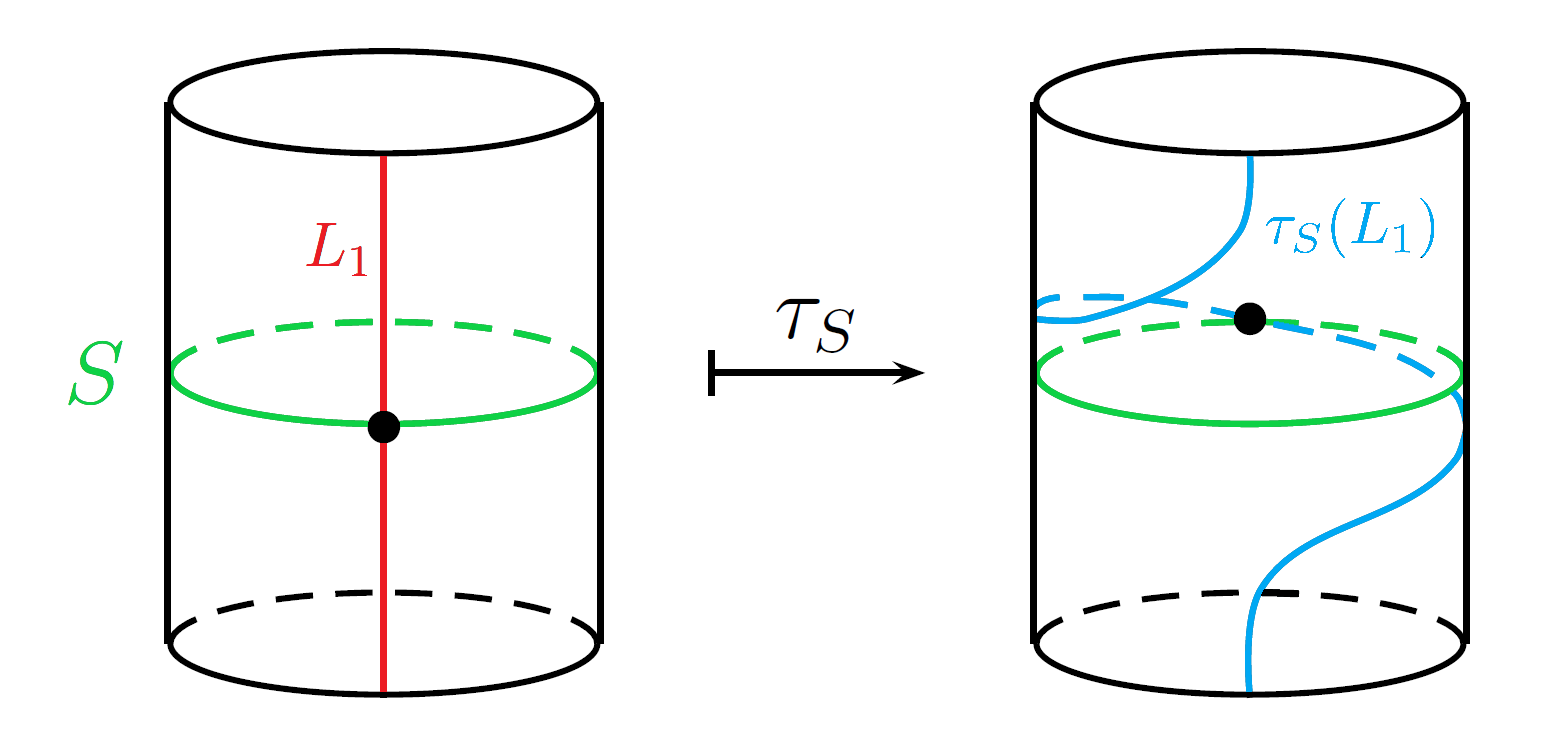
\includegraphics[width=0.8\linewidth]{fig10.png}
  \caption{沿球面 $S:=S_n$ 作用的 Dehn 扭转 $\tau_S$：所选纤维 $L_1$ 绕 $S$ 螺旋一周，并渐近地保持不变。\hfill（原书 p.100）}
  \label{fig:10}
\end{figure}

Dehn 扭转 $\tau_{S^n}$ 对 $T(\lambda)$ 的一条纤维的作用如图~\ref{fig:10} 所示。
有时便于通过要求 $h'|_{\mathbb R_{\ge0}}\ge0$、且只要“扭转速度” $h'$
超过某容差 $0<\varepsilon<1/2$ 就有 $h''<0$，来控制 $\tau_{S^n}$ 的
“摆动程度”。由此可以推断扭转后的纤维会在何处（横截地）与另一条未扭转的
纤维相交；若两条纤维的足点互为对径点，相交恰好发生在零截面上，正如图~\ref{fig:10}
所示（见 \cite{Sei02} 引理 1.9）。

我们把这一理论搬到流形层面。

\begin{Def}\label{def:6.22}
设 $M^{2n}=(M,\omega)$ 是辛流形。紧致拉格朗日子流形 $S^n\subset M$ 称为
\emph{拉格朗日球面}，若存在微分同胚 $f:S^n\to S$。它是\emph{标架的
（framed）}，若给定这样一些微分同胚的类 $[f]$，其中 $f_1\sim f_2$ 当且
仅当 $f_2^{-1}\circ f_1$ 可在 $\operatorname{Diff}(S^n)$ 内连续形变为
$O(n+1)$ 的某个正交矩阵。

对任意标架拉格朗日球面 $S=(S,[f])$ 可配一个 Dehn 扭转
$\tau_S\in\operatorname{Symp}(M,\omega)$。给定 $\lambda>0$，取任一代表
映射 $f:S^n\equiv T(0)\to S$ 并延拓到 $T(\lambda)$；后者经
$\iota:T(\lambda)\hookrightarrow M$ 辛嵌入 $M$，在 $T(\lambda)$ 内构造
支撑的 Dehn 扭转 \eqref{eq:6.90}。沿 $S$ 的 Dehn 扭转\footnote{读者不要被这里的记号迷惑：目前尚不知道
$[\tau_S]\in\pi_0(\operatorname{Symp}(M,\omega))$ 是否依赖于具体的类
$[f]$，尽管构造中其它所有选择实际上都无关紧要。为方便起见，我们不再
提及具体的标架 $[f]$，并隐含地把所有拉格朗日球面都视为已标架。}于是
为：
\begin{equation}
\tau_S(x):=
\begin{cases}
\iota\circ\tau_{S^n}\circ\iota^{-1}(x) & \text{若}\ x\in\operatorname{im}(\iota)\,,\\
x & \text{其它情形}\,.
\end{cases}
\label{eq:6.91}
\end{equation}
（具体地说，$\tau_S$ 是 $\phi^{2\pi}_H:M\setminus S\to M\setminus S$ 在
$S$ 上唯一可能的延拓，其中
$H:=h\circ\varrho\circ\iota^{-1}|_{\operatorname{im}(\iota)\setminus S}$
在 $M\setminus\operatorname{im}(\iota)$ 上为零。）特别地，$\tau_S$ 把
$S$ 对径地映到自身。
\end{Def}

% [Tutor Note: 【背景】定义 6.22 隐含使用了 Weinstein 拉格朗日邻域定理：
% 任何 $S\subset M$ 的邻域都辛同胚于 $T^*S^n$ 中零截面的邻域
% $T(\lambda)$。这正是可以把模型扭转 \eqref{eq:6.90} 搬到 $M$ 上的原因；
% 该定理见 \cite{Sil12} 定理 8.4。]

上一个定义隐含使用了 Weinstein 拉格朗日邻域定理（\cite{Sil12} 定理 8.4）：
$S\subset M$ 的任何邻域都辛同胚于 $S^n\equiv T(0)\subset T^*S^n$ 的
某个邻域 $T(\lambda)$（我们在命题 5.43 中也用过这一点）。

作为辛同胚，$\tau_S$ 把拉格朗日子流形映为拉格朗日子流形，并保持其全部
装饰（这一点并不平凡！）。换言之，$L\in\operatorname{obj}(\mathcal F(M))$
蕴含 $\tau_S(L)\in\operatorname{obj}(\mathcal F(M))$。我们关心的主要
结果是：

\begin{Thm}\label{thm:6.23}
设 $M$ 是辛流形，$\mathcal F(M)$ 是其相伴的 Fukaya 范畴。设
$S\in\operatorname{obj}(\mathcal F(M))$ 是拉格朗日球面，
$L\in\operatorname{obj}(\mathcal F(M))$ 是任意拉格朗日子流形。则
\begin{equation}
\tau_S(L)\cong T_S(L)=\operatorname{Cone}(\mathrm{ev})
\in\operatorname{obj}\bigl(\mathsf D^{\mathrm b}(\mathcal F(M))\bigr)\,,
\label{eq:6.92}
\end{equation}
其中 $T_S(L)$ 是 $L$ 沿 $S$ 的代数扭转，与
$\mathrm{ev}:CF(S,L)\otimes S\to L$ 的映射锥重合（如定义 4.21）。因此存在
正合三角形
\begin{equation}
\begin{tikzcd}[row sep=2.6em, column sep=3.4em]
HF(S,L)\otimes S \arrow[rr, "\langle \mathrm{ev}\rangle"] & & L \arrow[dl] \\
& \tau_S(L) \arrow[ul, "\langle\pi\rangle{[}1{]}"] \arrow[ur, "\langle c\rangle" swap] &
\end{tikzcd}
\label{eq:6.93}
\end{equation}
在 $\mathsf D^{\mathrm b}(\mathcal F(M))$ 中。于是，分别用
$HF(\tilde L,\square)$ 或 $HF(\square,\tilde L)$ 作用，给出长正合列
\[
\cdots\to\bigl(HF(S,L)\otimes HF(\tilde L,S)\bigr)^n
\xrightarrow{\langle\mu^2\rangle}HF^n(\tilde L,L)\to
HF^n(\tilde L,\tau_S(L))\xrightarrow{[1]}\cdots
\]
\[
\cdots\to HF^n(L,\tilde L)\to
\bigl(HF(S,L)\otimes HF(S,\tilde L)\bigr)^n
\xrightarrow{\langle d\rangle[1]}HF^{n+1}(\tau_S(L),\tilde L)\to\cdots
\]
对任意 $\tilde L\in\operatorname{obj}(\mathcal F(M))$ 成立；其中
$\mu^2$ 是 Floer 乘积，而 $\langle d\rangle$ 是一个复合，涉及典范同构
$HF(L,S)\cong HF(\tau_S(L),\tau_S(S))=HF(\tau_S(L),S)$ 与 Donaldson
“裤子”乘积。
\end{Thm}

\begin{proof}[证明（概要）]
这里只给出非常粗略的论证轮廓——精确证明是 Seidel 整篇论文
\cite{Sei02} 的内容。目标是先在 $A_\infty$-模层面工作，以便应用
引理 4.23。为保持一致，重记 $L_0:=S$、$L_1:=L$，并取
$L_2\in\operatorname{obj}(\mathcal F(M))$ 与 $\tau_{L_0}(L_1)$ 同痕；
由此定义 Floer 闭上链 $c\in CF(L_1,L_2)$（于是 $\mu^1(c)=0$）以及
$\mu^2(c,\,\cdot\,):CF(L_0,L_1)\to CF(L_0,L_2)$ 与零映射之间的链同伦
$k:CF(L_0,L_1)\to CF(L_0,L_2)[-1]$：
$\mu^1\circ k+k\circ\mu^1+\mu^2(c,\,\cdot\,)=0$。

在造出 \cite{Sei08} 引理 5.3 所需的适当附加数据之后（这在该书
(17d)--(17f) 各节中完成），引理 4.23 给出良定义的模同构
$t:T_{L_0}(\Upsilon(L_1))\to\Upsilon(L_2)$。还可改进此结果，把符号、
分次与膜结构一并纳入（\cite{Sei08} 定理 17.16）。因此
$T_{L_0}(\Upsilon(L_1))\cong\Upsilon(L_2)
\in\operatorname{obj}\bigl(H^0(\mathcal Q(M))\bigr)$。

现在借助注 4.22 第二个要点中的同构
$\mathcal T_{Y_0}(\tilde\Upsilon(Y_1))\cong
\tilde\Upsilon(\mathcal T_{Y_0}(Y_1))$ 过渡到扭复形。不妨设
$L_2=\tau_{L_0}(L_1)\in\operatorname{obj}(\operatorname{Tw}\mathcal F(M))$，
便得到
\[
\tilde\Upsilon(T_S(L))=\tilde\Upsilon(T_{L_0}(L_1))
\cong\mathcal T_{L_0}(\tilde\Upsilon(L_1))
\cong\tilde\Upsilon(\tau_{L_0}(L_1))=\tilde\Upsilon(\tau_S(L))\,,
\]
从而 $T_S(L)\cong\tau_S(L)\in\operatorname{obj}\bigl(\mathsf D^{\mathrm b}
(\mathcal F(M))\bigr)$（回忆 $\tilde\Upsilon$ 是拟等价）。

由图表 (89) 立即看出 $\tau_S(L)$ 嵌入正合三角形 \eqref{eq:6.93}；
其中我们辨认出 $c:L\to\tau_S(L)$ 恰是上面构造的 Floer 闭上链，而
$\langle\pi\rangle\in\hom_{\mathsf D^{\mathrm b}(\mathcal F(M))}
\bigl(\tau_S(L),(HF(S,L)\otimes S)[1]\bigr)\cong
\bigl(HF(S,L)\otimes HF(\tau_S(L),S)\bigr)^1\cong
\bigl(HF(S,L)\otimes HF(L,S)\bigr)^n$。此外，容易验证
$HF(\tilde L,\langle\mathrm{ev}\rangle)=\langle\mu^2\rangle$。关于 $d$
的确切定义，再次请读者参阅 \cite{Sei02}。
\end{proof}

% [Tutor Note: 【含糊】定理 6.23 的证明压缩了 Seidel 论文的整个主体：
% 链条是“$A_\infty$-模层面的模同构 $\Rightarrow$ 加符号/分次/膜结构
% $\Rightarrow$ 过渡到扭复形”。原文明确说精确证明是 \cite{Sei02} 的
% 内容，本译本不补。]

% [Tutor Note: 【易错】式 (92) 的 $\operatorname{Cone}(\mathrm{ev})$ 中
% $\mathrm{ev}:CF(S,L)\otimes S\to L$ 是“求值”态射，方向是
% $CF(S,L)\otimes S\to L$，不是反方向；相应的三角形 (93) 首项也因此写成
% $HF(S,L)\otimes S$。若把 $\mathrm{ev}$ 写成 $L\to CF(S,L)\otimes S$，
% 三个态射的次数都会错位。]

回顾扭映射锥通过 Yoneda 嵌入拟代表其抽象对应物，由定理 6.23 的证明还可
推出：

\begin{Cor}\label{cor:6.24}
设 $M$ 是辛流形，$\mathcal F(M)$ 是其相伴的 Fukaya 范畴。设
$S\in\operatorname{obj}(\mathcal F(M))$ 是拉格朗日球面，
$L\in\operatorname{obj}(\mathcal F(M))$ 是任意拉格朗日子流形。则 $L$ 沿
$S$ 的 Dehn 扭转 $\tau_S(L)\in\operatorname{obj}\bigl(\mathsf D^{\mathrm b}
(\mathcal F(M))\bigr)$ 拟代表 Yoneda 模
$\Upsilon(L)\in\operatorname{obj}(\mathcal Q(M))$ 沿 $S$ 的抽象代数扭转
$T_S(\Upsilon(L))\in\operatorname{obj}(\mathcal Q(M))$。
\end{Cor}

读者想必已经猜到，其背后的理论远比我们所触及的深刻——它围绕
Lefschetz 纤维化展开，而后者是 Picard--Lefschetz 理论的基本研究对象之一。
遗憾的是，详尽的研究超出我们的能力；感兴趣的读者可参阅 \cite{Sei08}
第三部分。

Fukaya 范畴的第二个有几何意义的侧面是所谓的\emph{拉格朗日手术}，其构造
在 \cite{FOOO07} 第 10.54 节中给出概要。先看另一件技术性准备。

\begin{Def}\label{def:6.25}
对满足 $|\varepsilon|>0$ 且足够小的 $\varepsilon\in\mathbb R$，考虑光滑
函数 $f_\varepsilon:\mathbb R^n\setminus\{0\}\to\mathbb R$，
$f_\varepsilon(x):=\varepsilon\log(\|x\|)$，以及它定义的 $1$-形式：
\[
df_\varepsilon(x)=\varepsilon\frac{x\cdot dx}{\|x\|^2}
=\sum_{j=1}^{n}y_j\,dx_j\in T^*_x(\mathbb R^n\setminus\{0\})\,,
\qquad y_j:=\varepsilon\frac{x_j}{\|x\|^2}\in\mathbb R\,.
\]
则 $H_\varepsilon:=\operatorname{graph}(df_\varepsilon)
=\{(x_1,y_1,\dots,x_n,y_n)\mid x\in\mathbb R^n\setminus\{0\}\}
\subset T^*(\mathbb R^n\setminus\{0\})\cong\mathbb C^n\setminus(i\mathbb R)^n$
是拉格朗日子流形，当 $\|x\|\to0$ 时渐近趋于 $(i\mathbb R)^n$（即
$0\in\mathbb R^n$ 上方的余切纤维），当 $\|x\|\to\infty$ 时渐近趋于零截面
$\mathbb R^n$；其中与复空间的等同由 $z_j:=x_j+iy_j\in\mathbb C$ 给出。

注意，若记 $r:\mathbb C^n\to\mathbb C^n$ 为沿对角线的反射
（$x_j+iy_j\mapsto y_j+ix_j$，$j=1,\dots,n$），则 $r(H_\varepsilon)
=H_\varepsilon$（事实上，构造的对称性说明 $H_\varepsilon$ 也是镜像图像，
由一切满足 $y\in\mathbb R^n\setminus\{0\}$ 且
$x_j=\varepsilon y_j/\|y\|^2$ 的 $(y_1,x_1,\dots,y_n,x_n)\in
T^*(\mathbb R^n\setminus\{0\})$ 组成）。

再取修正用的光滑函数 $g\in C^\infty(\mathbb R_{>0})$，使得当
$0<x\le x_0$ 时 $g(x)=\log(x)-|\varepsilon|$，其中
$x_0\equiv x_0(|\varepsilon|)$ 足够小；当 $x\ge 2x_0$ 时 $g$ 为常数，
且 $g'\ge0$、$g''\le0$（与引理 6.20 中的映射 $h$ 比较）。定义调整后的
光滑函数
\[
\tilde f_\varepsilon:\mathbb R^n\setminus\{0\}\to\mathbb R\,,\qquad
\tilde f_\varepsilon(x):=\varepsilon g(\|x\|)=
\begin{cases}
f_\varepsilon(x)-\varepsilon|\varepsilon| & \text{若}\ 0<x\le x_0\,,\\
\text{常数} & \text{其它情形}\,,
\end{cases}
\]
并考察其图像 $\tilde H_\varepsilon:=\operatorname{graph}(d\tilde f_\varepsilon)
\subset T^*(\mathbb R^n\setminus\{0\})$；它仍是拉格朗日子流形，且在反射
$r$ 下不变。特别地，在 $0$ 处半径为 $2x_0$ 的 $n$ 维复球
$B^n_{2x_0}(0)\subset\mathbb C^n$ 之外，
$\tilde H_\varepsilon=\mathbb R^n\cup(i\mathbb R)^n$。
\end{Def}

% [Tutor Note: 【易错】$f_\varepsilon=\varepsilon\log\|x\|$ 的符号决定
% 手术“从哪一侧”光滑化：$H_\varepsilon$ 在 $\|x\|\to0$ 时贴到余切纤维
% $(i\mathbb R)^n$ 上、在 $\|x\|\to\infty$ 时贴到零截面 $\mathbb R^n$ 上。
% 因此 $L_1\#_\varepsilon L_2=L_2\#_{-\varepsilon}L_1$：交换次序必须同时
% 把 $\varepsilon$ 变号。这正是后文强调 $L_2\#_\varepsilon L_1$ 连同痕
% 都不对的原因。]

\begin{Def}\label{def:6.26}
设 $M^{2n}=(M,\omega)$ 是辛流形，$\mathcal F(M)$ 是其相伴的 Fukaya 范畴。
设 $L_1,L_2\in\operatorname{obj}(\mathcal F(M))$ 在某个 $p\in M$ 处横截
相交。取适当的 Darboux 坐标卡\footnote{这是局部坐标
$(x^j,y^j)_{j=1}^n$，使 $\omega|_U=\sum_{j=1}^n dx^j\wedge dy^j$；
由 \cite{Sil12} 定理 8.1，这样的坐标卡总是存在。}
$\psi:U\subset M\to V\subset\mathbb R^{2n}\cong\mathbb C^n$，定义在 $p$
的邻域 $U$ 上、以 $p$ 为中心（故 $\psi(p)=0$）；可把两条拉格朗日子流形
摆成 $\psi(L_1\cap U)=\mathbb R^n\cap V$ 与
$\psi(L_2\cap U)=(i\mathbb R)^n\cap V$。

现在按定义 6.25 构造 $\tilde H_\varepsilon$，并调整 $\varepsilon$ 使
$B^n_{2x_0}(0)\subset\psi(U)$。于是
\begin{equation}
L_1\#_\varepsilon L_2:=
\begin{cases}
(L_1\cup L_2)\setminus U & \text{在}\ M\setminus U\ \text{上}\,,\\
\psi^{-1}(\tilde H_\varepsilon)\cap U & \text{在}\ U\ \text{上}\,,
\end{cases}
\label{eq:6.94}
\end{equation}
称为 $L_1$ 与 $L_2$ 在 $p$ 处的\emph{拉格朗日连通和}（或\emph{拉格朗日
手术}），有时简记为 $L_1\#L_2$。它是 $M$ 的拉格朗日子流形，继承全部
所需的装饰（这一点并不平凡！），即 $L_1\#_\varepsilon L_2
\in\operatorname{obj}(\mathcal F(M))$。区域
$(L_1\#_\varepsilon L_2)\cap U=\psi^{-1}(\tilde H_\varepsilon)\cap U$
称为\emph{拉格朗日把手}。
\end{Def}

二维情形如图~\ref{fig:11} 所示，四维情形可参阅 \cite{AS09} 第 3 节。

由上述构造可知 $L_1\#_\varepsilon L_2=L_2\#_{-\varepsilon}L_1$（而不是
$L_2\#_\varepsilon L_1$，后者甚至不同痕于 $L_1\#_\varepsilon L_2$！）。
此外，只要 $\operatorname{sgn}(\varepsilon)=\operatorname{sgn}(\delta)$，
$L_1\#_\varepsilon L_2$ 就哈密顿同痕于某个 $L_1\#_\delta L_2$（在拉格朗日
把手的适当管状邻域中计算即可看出）。然而，若在多个不同点作手术，最终
结果就失去同痕不变性。

% [Tutor Note: 【含糊】“在拉格朗日把手的适当管状邻域中计算”省略了
% $L_1\#_\varepsilon L_2$ 与 $L_1\#_\delta L_2$ 之间的显式哈密顿同痕；
% 其要点是把 $\varepsilon$ 连续形变到同号的 $\delta$（保持
% $|\varepsilon|>0$ 足够小），并让调整函数 $g$ 随之连续变化。]

\begin{figure}[htbp]
  \centering
  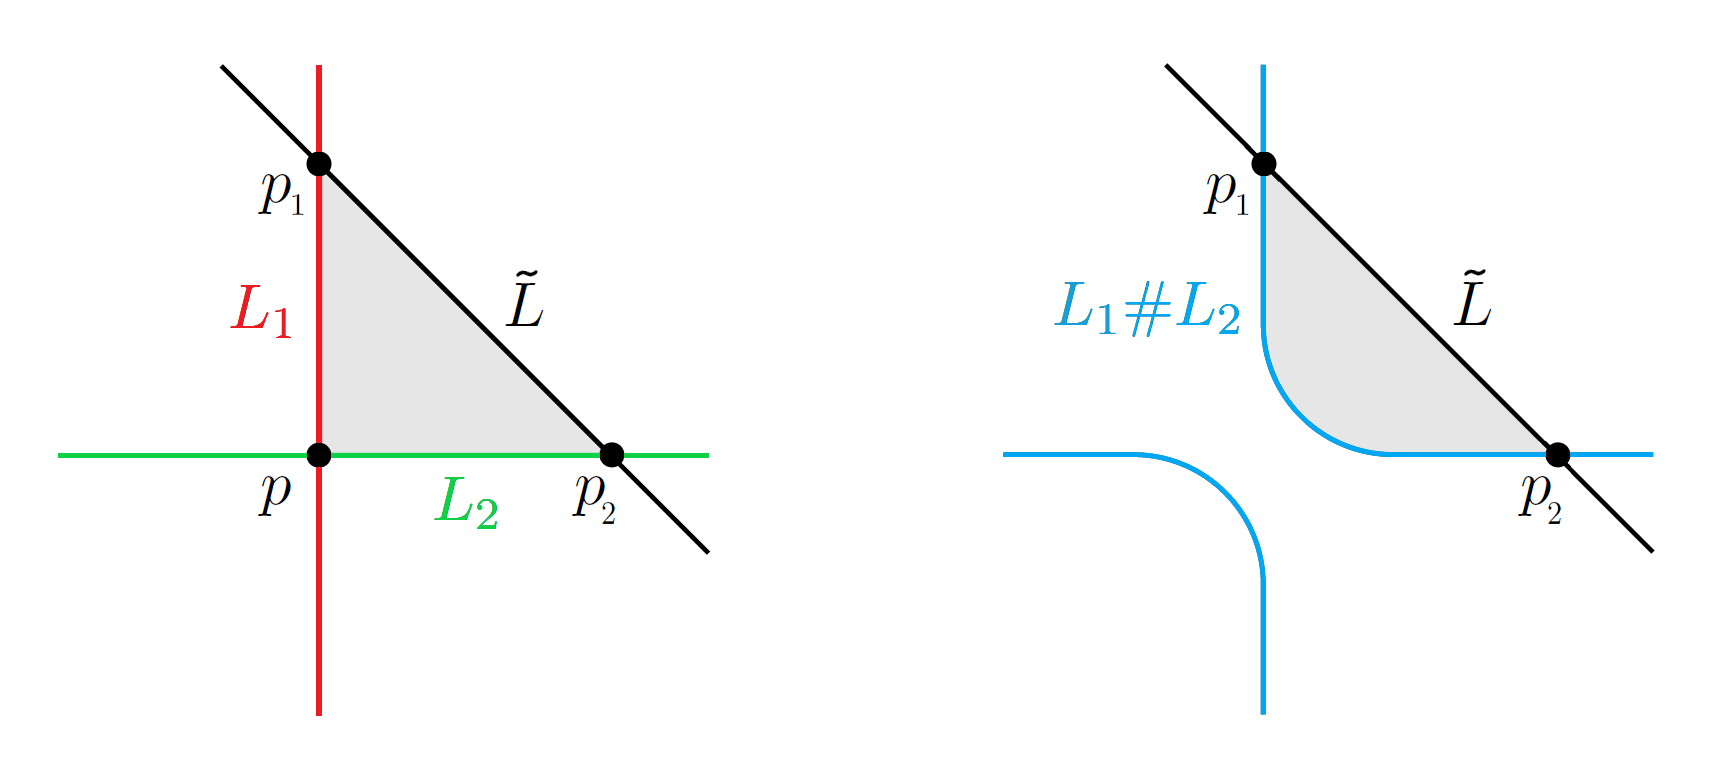
\includegraphics[width=0.8\linewidth]{fig11.png}
  \caption{两个一维拉格朗日子流形 $L_1,L_2\subset M^2$ 在 $p\in M$ 处横截相交时的拉格朗日连通和 $L_1\#L_2$；在 $0\in\mathbb C$ 的某个邻域内，经适当的 Darboux 坐标卡，它们分别映为实轴与虚轴。$L_1\#L_2$ 的“弯曲区域”即所谓的拉格朗日把手。\hfill（原书 p.103）}
  \label{fig:11}
\end{figure}

\begin{Rem}\label{rem:6.27}
取 $L_2=S\in\operatorname{obj}(\mathcal F(M))$ 为拉格朗日球面，与 $L_1$
在唯一一点 $p$ 处横截相交。则 $L_1\#S$ 哈密顿同痕于 Dehn 扭转
$\tau_S(L_1)$：
\begin{equation}
L_1\#S\simeq\tau_S(L_1)
\label{eq:6.95}
\end{equation}
（与图~\ref{fig:10} 比较）。因此，$S$ 调控扭转，而 $L_1$ 支配渐近行为。在二维情形，
$L_1$ 的局部 Darboux 图像对应虚直线 $i\mathbb R$，$S$ 的局部图像对应以
$1\in\mathbb C$ 为圆心的 $S^1$。于是拉格朗日手术相当于把 $S^1$ 与
$i\mathbb R$ 之间在 $0$ 附近被挤压的角形区域磨光。这可非正式地看作产生
拉格朗日连通和的一般配方。
\end{Rem}

% [Tutor Note: 【易错】式 (95) 中 $\simeq$ 表示哈密顿同痕，而非同构；
% $L_1\#S$ 与 $\tau_S(L_1)$ 只是同痕的拉格朗日子流形，在 $\mathcal F(M)$
% 的上同调范畴中才成为同构对象。原文在此用了 $\simeq$ 而非 $\cong$，
% 译文保留这一区别。]

与 Dehn 扭转类似，拉格朗日连通和与扭映射锥密切相关：

\begin{Thm}\label{thm:6.28}
设 $L_1,L_2\in\operatorname{obj}(\mathcal F(M))$ 在唯一一点 $p\in M$ 处
横截相交，于是 $p$ 必然是 $CF(L_2,L_1)$ 的 Floer 闭上链。\footnote{这由
Floer 复形与微分的定义立得：$\mu^1$ 是 $1$ 次的，故不可能保持
$\mathcal X(L_2,L_1)$ 中唯一的生成元 $p$。}再取第三条
$\tilde L\in\operatorname{obj}(\mathcal F(M))$，使交点满足
$\tilde L\cap(L_1\#_\varepsilon L_2)=(\tilde L\cap L_1)\cup
(\tilde L\cap L_2)$（当 $|\varepsilon|$ 足够小时可行；参看图~\ref{fig:11}）。记
$p_i$ 为 $\tilde L\cap L_i$ 中的横截交点。则对由 $\tilde L$ 与
$L_1\#_\varepsilon L_2$ 所围区域上适当的近复结构
$J\in\mathcal J(M,\omega)$，存在双射
\[
\left\{\begin{array}{c}
\text{以}\ \tilde L\ \text{与}\ L_1\#_\varepsilon L_2\ \text{为边界}\\
\text{从}\ p_2\ \text{到}\ p_1\ \text{的}\ J\text{-全纯条带}
\end{array}\right\}
\longleftrightarrow
\left\{\begin{array}{c}
\text{以}\ \tilde L,L_1,L_2\ \text{为边界，从}\ p_2\ \text{经}\ p_1\\
\text{到}\ p\ \text{的}\ J\text{-全纯三角形}
\end{array}\right\}.
\]
作为推论，$CF(\tilde L,L_1\#_\varepsilon L_2)$ 是
$\mu^2(p,\,\cdot\,):CF(\tilde L,L_2)\to CF(\tilde L,L_1)$ 的标准映射锥
（在上链复形意义下），于是嵌入短正合列
\[
\{0\}\to CF(\tilde L,L_1)\to CF(\tilde L,L_1\#_\varepsilon L_2)
\to CF(\tilde L,L_2)\to\{0\}\,,
\]
它诱导长正合列
\begin{equation}
\begin{aligned}
\cdots\to HF^n(\tilde L,L_1)&\to HF^n(\tilde L,L_1\#_\varepsilon L_2)
\to HF^n(\tilde L,L_2)\\
&\xrightarrow{\langle\mu^2(p,\,\cdot\,)\rangle[1]}\cdots\,.
\end{aligned}
\label{eq:6.96}
\end{equation}
事实上存在正合三角形
\begin{equation}
\begin{tikzcd}[row sep=2.6em, column sep=3.4em]
L_2 \arrow[rr, "\langle p\rangle"] & & L_1 \arrow[dl] \\
& L_1\#_\varepsilon L_2 \arrow[ul, "\langle\pi\rangle{[}1{]}"] \arrow[ur, "\langle i\rangle" swap] &
\end{tikzcd}
\label{eq:6.97}
\end{equation}
在 $\mathsf D^{\mathrm b}(\mathcal F(M))$ 中，也就是说
\begin{equation}
L_1\#_\varepsilon L_2\cong\operatorname{Cone}(p)
\in\operatorname{obj}\bigl(\mathsf D^{\mathrm b}(\mathcal F(M))\bigr)\,.
\label{eq:6.98}
\end{equation}
\end{Thm}

% [Tutor Note: 【易错】三角形 (97) 的方向是 $L_2\xrightarrow{\langle p\rangle}L_1
% \xrightarrow{\langle i\rangle}L_1\#_\varepsilon L_2$，即映射锥的“第一项”
% 是 $L_2$ 而不是 $L_1$；这与 (98) 中 $\operatorname{Cone}(p)$ 的次序一致。
% 若把 $p$ 看成 $CF(L_1,L_2)$ 的元素，三角形要整体反向，易生混淆。]

该结果的证明贯穿 \cite{FOOO07} 第 10.59--10.62 节（那里称之为
“定理 Z”）。为研究由 $L_1\#_\varepsilon L_2$ 与 $\tilde L$ 界定的
$J$-全纯条带所对应的模空间
$\mathcal M(p_2,p_1;[u],J,H)$，该证明大量依赖我们在第 5 章偶尔提及的
分析工具以及粘接技巧，并利用了复空间 $\mathbb C^n$ 中的局部构造。

\begin{Rem}\label{rem:6.29}
仍取 $L_2=S\in\operatorname{obj}(\mathcal F(M))$ 为拉格朗日球面，使
$L_1\#S\simeq\tau_S(L_1)$。于是定理 6.28 的断言与定理 6.23 的断言相容。
事实上，把连接同态
$\langle\mu^2\rangle:HF(S,L_1)\otimes HF(\tilde L,S)\to HF(\tilde L,L_1)$
的输入固定为 $\langle p\rangle\in HF(S,L_1)$（并重记 $L:=L_1$）之后，
\eqref{eq:6.93} 诱导的长正合列正是 \eqref{eq:6.96}。同样，图表
\eqref{eq:6.93} 取 \eqref{eq:6.97} 的形状。
\end{Rem}

最后提醒一点：把 Dehn 扭转与拉格朗日连通和等同于扭映射锥，是一把双刃剑：
代数对象与几何对象之间这种词典的好处，部分被处理高阶 Floer 复合映射
$\mu^d$ 的必要性所抵消——想想作多次手术时图~\ref{fig:11} 的局部图像。因此，
研究拉格朗日构件（constituents）不可避免地要求我们增强手头的分析工具。
这超出本书范围；我们不再深入。

最后给出关于分裂封闭 $\mathsf D^\pi(\mathcal F(M))$ 之重要性的一些启发。
给定有限多条拉格朗日子流形 $L_i\in\operatorname{obj}(\mathcal F(M))$，
它们生成 $A_\infty$-子范畴 $\mathcal A\subset\mathcal F(M)$；则
$A_\infty$-范畴 $\operatorname{Tw}\mathcal A$ 包含由它们迭代可构造的
一切映射锥，特别是 Dehn 扭转与拉格朗日连通和。对全部初始对象作手术，
可能产生一条不连通的拉格朗日子流形。它虽是 $\mathcal A$ 的元素，其连通
分支却未必还是 $\mathcal A$ 的元素。因此人们猜想：取
$\operatorname{Tw}\mathcal A$ 的幂等完备化，可以把各个构件作为
$\mathsf D^\pi(\mathcal A)$ 的对象纳入，从而弥补这一缺陷。在环面的情形，
这一点尤其成立：

\begin{Ex}\label{ex:6.30}
考虑辛环面 $\mathbb T^2=S^1\times S^1$，配以标准面积形式
$\omega:=d\theta_1\wedge d\theta_2$，其中 $\theta_1$ 与 $\theta_2$ 是
相应因子 $S^1\subset\mathbb C$ 上的角坐标。\footnote{注意
$\theta_j(e^{2\pi it}):=t\in(0,1)$ 只在 $S^1\setminus\{1\}$ 上良定义，
并非整体定义，因此 $d\theta_j$ 并非由 $\theta_j$ 的外微分所得的
$1$-形式！}$\mathcal F(\mathbb T^2)$ 的对象（即带装饰的拉格朗日子流形）
是 $\mathbb T^2$ 上的一切\emph{简单环路}（即不自交的闭道路），可等同于
$\mathbb Z\oplus\mathbb Z=\pi_1(\mathbb T^2)$ 的类代表元，并由其在
$\mathbb T^2$ 的商空间表示中的有理斜率（同伦意义下）决定。

取定一条经线方向的环路 $L_1:=\alpha\in\operatorname{obj}(\mathcal F(\mathbb T^2))$
与一条纬线方向的环路 $L_2:=\beta\in\operatorname{obj}(\mathcal F(\mathbb T^2))$，
它们分别沿着 $\mathbb T^2$ 的等同多边形的两个因子（图~\ref{fig:12} 左上）；它们
属于 $\pi_1(\mathbb T^2)$ 的类 $(1,0)$ 与 $(0,1)$。记
$p\in CF(L_2,L_1)$ 为 $\alpha$ 与 $\beta$ 的唯一交点。由于 $\beta$
显然微分同胚于 $S^1$，它是拉格朗日球面，故可构造 $\alpha$ 沿它的 Dehn
扭转。由注 6.27 与定理 6.28，这给出新的简单环路
$\tau_\beta(\alpha)\simeq\alpha\#\beta\cong\operatorname{Cone}(p)
\in\operatorname{obj}\bigl(\mathsf D^{\mathrm b}(\mathcal F(\mathbb T^2))\bigr)$，
如图~\ref{fig:12} 右上所示。Dehn 扭转过程可以无限迭代（这相当于第 4.4 节所讨论的
反复取代数扭转），并同样可沿 $\alpha$ 施加 $\tau_\alpha$。

由于我们将遍历 $\pi_1(\mathbb T^2)$ 的所有同伦类——事实上
$\tau_\alpha,\tau_\beta\in\operatorname{Diff}(\mathbb T^2)$ 生成
$\mathbb T^2$ 的映射类群，即其微分同胚的环境同痕类——人们自然会期待
由此得到 $\mathcal F(\mathbb T^2)$ 的全部对象；但事实远非如此：取
$\nu\in\Omega^1(\mathbb T^2\setminus\{p\})$ 使 $d\nu=\omega$
（在挖去一点的环面上这是可行的），且
$\int_\alpha\nu=\int_\beta\nu=0$，这意味着
$\alpha,\beta\subset\mathbb T^2$ 是\emph{平衡的}（或\emph{正合的}）
拉格朗日子流形，且 $\nu|_\alpha=d\theta_\alpha$、$\nu|_\beta=d\theta_\beta$
（于是确实 $\int_\alpha\nu=\int_\alpha d\theta_\alpha
=\theta_\alpha(e^{2\pi i})-\theta_\alpha(e^0)=0$，对 $\beta$ 同理）。
那么上面构造的一切后续映射锥也将是正合的：观察图~\ref{fig:12} 左上中的
$\tau_\beta(\alpha)$，可见它在 $[0,1]\times[0,1]$ 上的双射性使其所描述的
Dehn 扭转后的拉格朗日子流形为正合——换个说法，若沿相应的简单环路追踪
（见图~\ref{fig:12}），会看到它绕每个因子恰好一周（事实上
$\tau_\beta(\alpha)$ 代表 $(1,1)\in\pi_1(\mathbb T^2)$）。这显然是我们
需要去除的限制，因为并非所有简单环路都正合！

\begin{figure}[htbp]
  \centering
  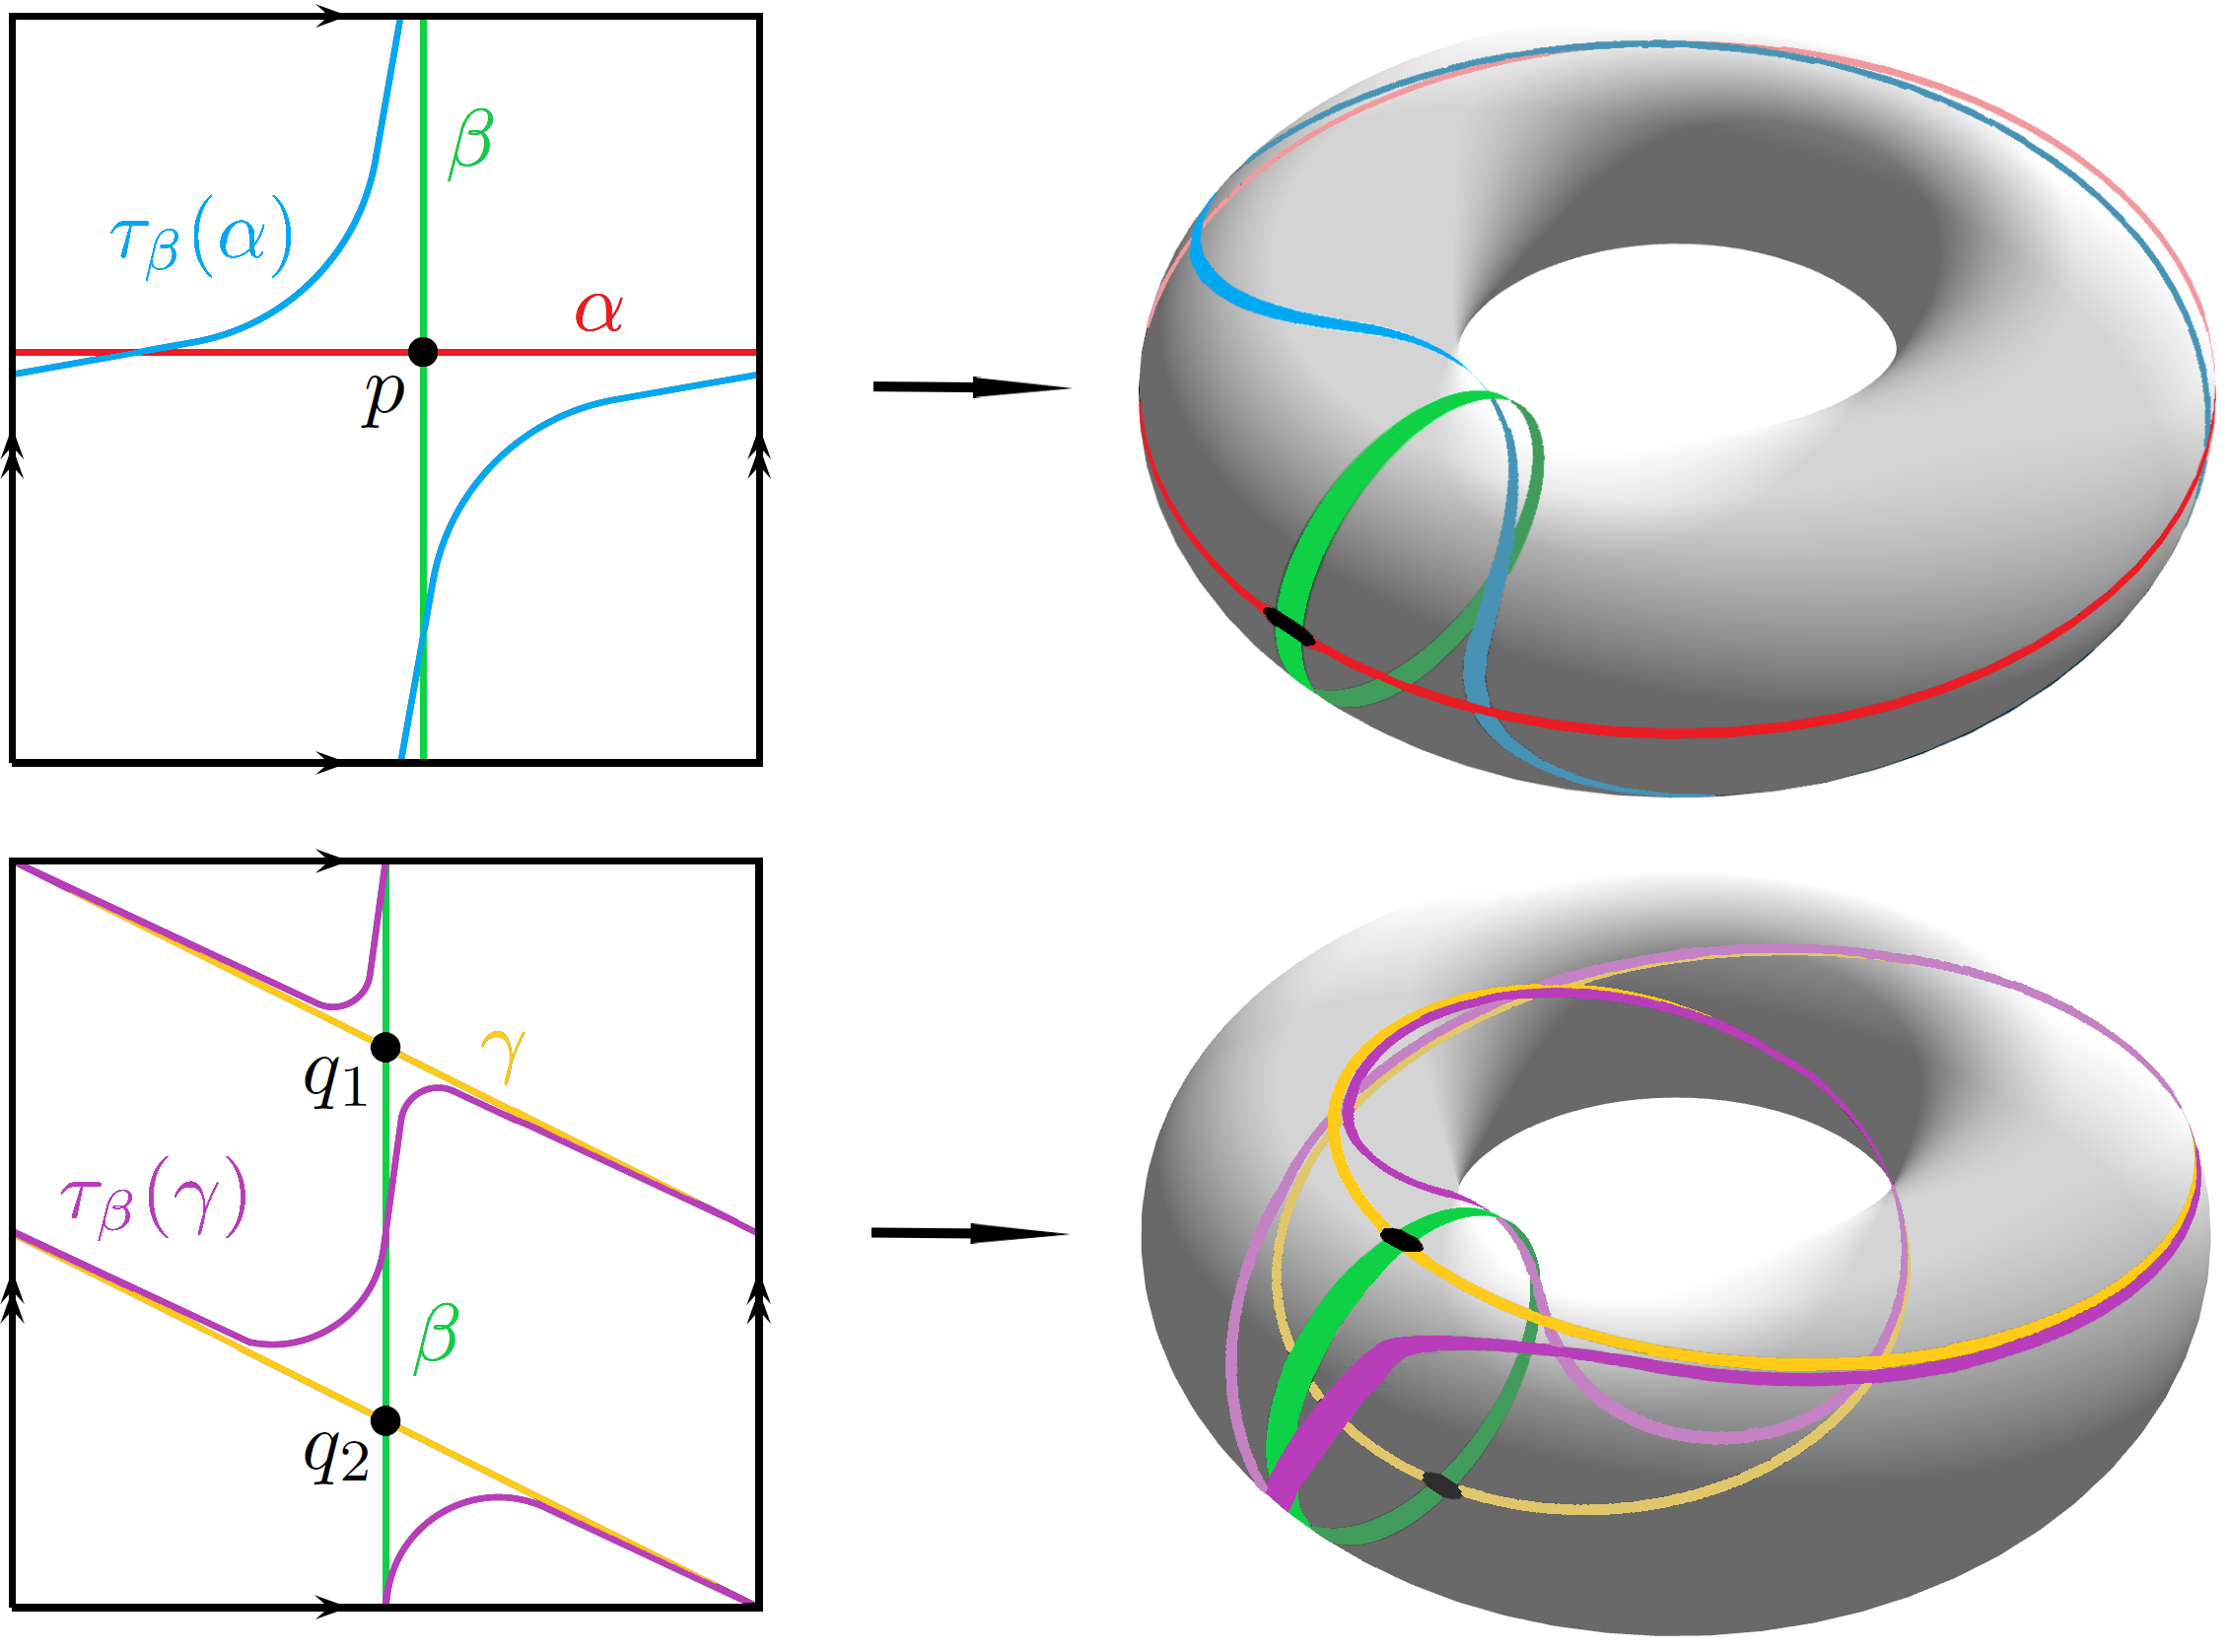
\includegraphics[width=0.85\linewidth]{fig12.png}
  \caption{两个简单闭曲线的拉格朗日连通和可能给出非平衡简单闭曲线的直和（下排）。它们是分裂封闭导出范畴 $\mathsf D^\pi(\mathcal F(T^2))$ 的真正对象。\hfill（原书 p.106）}
  \label{fig:12}
\end{figure}

例如，考虑第三条简单环路
$L_3:=\gamma\in\operatorname{obj}(\mathcal F(\mathbb T^2))$，其有理斜率为
$-1/2$（图~\ref{fig:12} 左下），代表类 $(2,1)\in\pi_1(\mathbb T^2)$（即
$\tau_\alpha(\tau_\alpha(\beta))$ 的类）；它与 $\beta$ 相交两次，设交点为
$q_1,q_2\in CF(L_2,L_3)$。构造 $\gamma$ 与 $\beta$ 的（二重）连通和，
并小心应用定理 6.28，可得
$\tau_\beta(\gamma)\simeq\gamma\#\beta
\cong\operatorname{Cone}(T^{w_1}q_1+T^{w_2}q_2)$ 在
$\mathsf D^{\mathrm b}(\mathcal F(\mathbb T^2))$ 中成立，其中权重
$w_1,w_2\in\mathbb R$ 适当。其几何结果恰是图~\ref{fig:12} 右下那两条紫色的、
非正合简单环路之直和，它们都落在 $\alpha$ 的同伦类 $(1,0)$ 中。用心的
读者已经知道下一步：取 $\mathcal F(\mathbb T^2)$ 的分裂封闭，从而把
映射锥的两个直和项都作为 $\mathsf D^\pi(\mathcal F(\mathbb T^2))$ 的
对象纳入。

总之，通过沿 $\alpha$ 与 $\beta$ 反复扭转并最终纳入出现的直和项，可以
得到 $\mathbb T^2$ 的一切简单环路（在哈密顿同痕意义下）。更系统的讨论见
\cite{LP11}，尤其侧重拉格朗日手术与由此产生的正合三角形。我们的处理旨在
为下一个结果提供几何直观。
\end{Ex}

% [Tutor Note: 【易错】$\operatorname{Cone}(T^{w_1}q_1+T^{w_2}q_2)$ 中
% 的 $T^{w_i}$ 是 Novikov 系数（$T$ 是 Novikov 变量），权重
% $w_1,w_2\in\mathbb R$ 来自两条条带的辛面积；它不是拓扑对象，而是
% 打点计数中的指数权。若把 $T^{w_i}$ 误读为“$T$ 的 $w_i$ 次幂算子”，
% 会误以为这是某种几何运算。]

\begin{Pro}\label{pro:6.31}
辛 $2$-环面 $\mathbb T^2=S^1\times S^1$ 的任意一对经线与纬线都分裂生成
其 Fukaya 范畴 $\mathcal F(\mathbb T^2)$。因此，任何微分同胚于
$\mathbb T^2$ 的紧致 $2$ 维辛流形 $M^2$，其 Fukaya 范畴 $\mathcal F(M)$
都被任意一对经线与纬线同构地分裂生成。
\end{Pro}

\begin{proof}[证明（概要）]
我们直接在 $M$ 上工作。设 $S_1,S_2\in\operatorname{obj}(\mathcal F(M))$
分别微分同胚于上一例中固定的经线与纬线。取任一同伦本质的闭曲线（即
$\mathbb T^2$ 中简单环路的流形类比）。我们要证明它落在 $\{S_1,S_2\}$
的分裂封闭中，于是整个 Fukaya 范畴 $\mathcal F(M)$ 也如此。

首先可以证明，对所有 $k\ge1$ 都有
$(\tau_{S_1}\circ\tau_{S_2})^{6k}=1\in SL(2,\mathbb Z)$。于是存在典范
态射 $i:L\to(\tau_{S_1}\circ\tau_{S_2})^{6k}(L)\cong L$，它嵌入
$\mathsf D^{\mathrm b}(\mathcal F(M))$ 中的图表
\[
\begin{tikzcd}[row sep=2.6em, column sep=3.6em]
Y \arrow[rr] & & L \arrow[dl, "\langle i\rangle"] \\
& (\tau_{S_1}\circ\tau_{S_2})^{6k}(L) \arrow[ul] &
\end{tikzcd}
\]
其中由三角范畴的公理 (T1)，可找到某个
$Y\cong\operatorname{Cone}(i)\in\operatorname{obj}\bigl(\mathsf D^{\mathrm b}
(\mathcal F(M))\bigr)$ 补全正合三角形。注意由命题 5.43，
$\langle i\rangle\in HF^0(L,L)\cong H^0(L)$ 只是一个奇异上同调类。
若它为零，则由注 3.48 的讨论立即推出
$\operatorname{Cone}(i)\cong L\oplus L$，从而 $L$ 是一个直和项，必被纳入
$\{S_1,S_2\}$ 的分裂封闭中，正如所断言。

可以证明，若取 $k=2$，则 $\langle i\rangle=0$。然而其背后的论证对我们
所发展的有限工具而言过于曲折。读者可参阅 \cite{AS09} 命题 6.1 以了解
主要策略的概要。
\end{proof}

% [Tutor Note: 【含糊】“对所有 $k\ge1$ 有 $(τ_{S_1}∘τ_{S_2})^{6k}=1\in SL(2,Z)$”
% 依赖映射类群 $MCG(\mathbb T^2)=SL(2,\mathbb Z)$ 中两个 Dehn 扭转生成元
% 的关系 $(\tau_\alpha\tau_\beta)^6=1$；原文未给证明。取 $k=2$ 时
% $\langle i\rangle=0$ 更只是引用 \cite{AS09} 命题 6.1，本译本不补写。]

\subsection{wrapped Fukaya 范畴}\label{sec:6.5}

作为本章的结束，我们简要而颇为含糊地讨论 Fukaya 范畴的 wrapped 版本，
它处理正合辛流形（回忆第 5.8 节的设定）。其主要优点是：我们不再需要
要求正合拉格朗日子流形紧致，只需其在无穷远处有某种行为。我们仍按
\cite{Aur13} 第 4.1 节的纲要进行，并参照 \cite{Abo10} 第 2 节。先补充
一些工作工具（见 \cite{Sil12}）。

\begin{Def}\label{def:6.32}
设 $M^n$ 是光滑流形。点 $p\in M$ 称为\emph{接触点}，若它有一个切超平面
$H_p\subset T_pM$，即维数为 $\dim(H_p)=n-1$ 的子空间。

给定光滑截面 $H\in\Gamma(TM)$（\emph{接触分布}），$p\mapsto H_p$；
局部可写作 $H=\ker(\alpha)$，其中 $\alpha\in\Omega^1(M)$ 不唯一，且
$d\alpha|_H$ 是辛形式。于是每个 $H_p$ 都是某个线性映射
$0\neq\alpha_p:T_p\to\mathbb R$ 的核。我们称 $\alpha$ 为 $M$ 上的
\emph{接触形式}。其非退化性迫使 $M$ 的维数 $n$ 为奇数。
\end{Def}

\begin{Def}\label{def:6.33}
正合辛流形 $M^{2n}=(M,\omega)$（$\omega=d\lambda\in\Omega^2(M)$）称为
\emph{Liouville 流形}，若它配有某个完备的 $Z\in\mathfrak X(M)$，该向量场
在无穷远处向外（见下一段），并满足 $\iota_Z(\omega)=\lambda$，或等价地
$\mathcal L_Z(\omega)=\omega$。此时 $Z$ 称为与 Liouville 形式
$\lambda\in\Omega^1(M)$ 相伴的\emph{Liouville 向量场}。
\end{Def}

我们特别关心这样的 Liouville 流形 $(M^{2n},\omega=d\lambda)$：它含有某个
紧致区域 $M^{in}\subset M$，具有如下性质（见图~\ref{fig:13}）：
\begin{itemize}
  \item $(2n-1)$ 维边界 $\partial M^{in}$ 是光滑超曲面，配有接触形式
  $\alpha:=\lambda|_{\partial M^{in}}\in\Omega^1(\partial M^{in})$；
  \item $\operatorname{zeros}(Z)\subset M^{in}$，且 $Z$ 正横截于
  $\partial M^{in}$，即对一切 $x\in\partial M^{in}$ 有
  $Z(x)\notin T_x(\partial M^{in})$ 且 $Z(x)(x^1)>0$（在 $x$ 周围的适当
  半空间坐标卡中）。
\end{itemize}

$Z$ 的流 $\phi^t_Z:M\to M$ 使我们能把 $M\setminus M^{in}$ 等同于
辛化 $[1,\infty)\times\partial M^{in}$：其中给定径向坐标函数
$r\in C^\infty([1,\infty))$，有
$Z=r\frac{\partial}{\partial r}$ 与 $\lambda=r\alpha$。滥用记号，我们可以
非正式地把 Liouville 流形写成粘合空间
\begin{equation}
M=M^{in}\sqcup_{\partial M^{in}}\bigl([1,\infty)\times\partial M^{in}\bigr)\,.
\label{eq:6.99}
\end{equation}
为后文之用，记 $\psi^\rho_Z:=\phi^{\log\rho}_Z$ 为 $Z$ 的时间
$\log\rho$ 流（$\rho>1$）；注意 $\phi^t_Z$ 是共形辛的，故
$\psi^\rho_Z\in\operatorname{Symp}(M,\omega)$。

% [Tutor Note: 【易错】$M\setminus M^{in}\cong[1,\infty)\times\partial M^{in}$
% 中的坐标 $r$ 满足 $Z=r\,\partial/\partial r$、$\lambda=r\alpha$；因此
% 时间 $t$ 的流把 $r$ 变成 $e^t r$，从而 $\psi^\rho_Z=\phi^{\log\rho}_Z$
% 把 $r$ 乘以 $\rho$。这个“时间–半径”对应在定义 $\mu^2_{W(M)}$ 的
% 重标度（$\rho=2$）时反复用到。]

\begin{figure}[htbp]
  \centering
  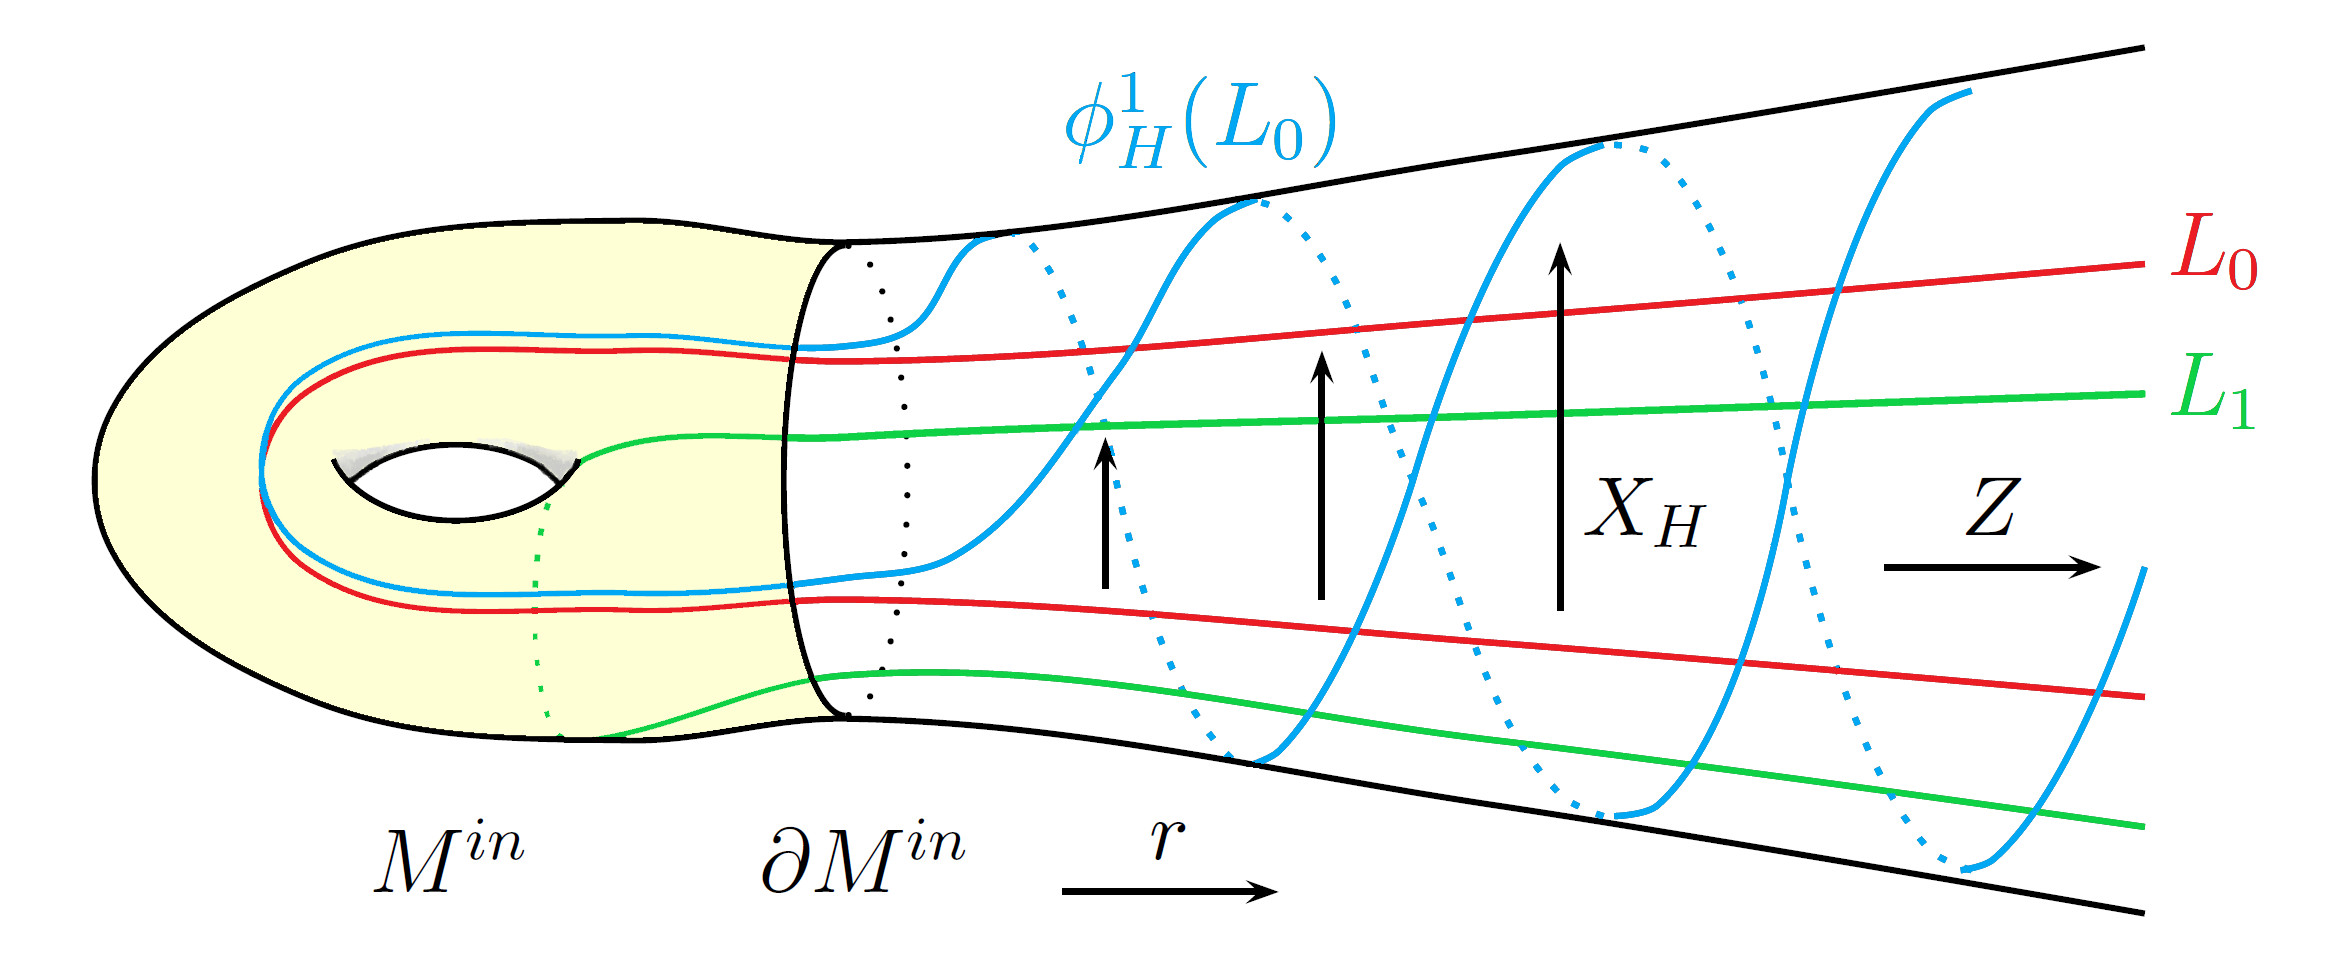
\includegraphics[width=0.8\linewidth]{fig13.png}
  \caption{Liouville 二维流形 $M$ 的正合拉格朗日子流形 $L_0,L_1\in\operatorname{obj}(\mathcal W(M))$。“卷绕哈密顿量” $H\in C^\infty(M)$（在 $M$ 的某紧子集之外为二次型）的流使 $L_0$ 沿径向向外螺旋。\hfill（原书 p.108）}
  \label{fig:13}
\end{figure}

给定如上所述的 Liouville 流形 $(M^{2n},\omega=d\lambda)$（且
$2c_1(TM)=0$），其 \emph{wrapped Fukaya 范畴} $\mathcal W(M)$ 是如下
构造的 $A_\infty$-范畴（更从容的探讨见 \cite{Abo10}）：

\begin{itemize}
  \item $\operatorname{obj}(\mathcal W(M))$ 中的对象是按第 5 章意义适当
  装饰的连通正合拉格朗日子流形
  \begin{equation}
  L=L^{in}\sqcup_{\partial L^{in}}\bigl([1,\infty)\times\partial L^{in}\bigr)
  \subset M
  \label{eq:6.100}
  \end{equation}
  （“在无穷远处为锥形”），其中 $L^{in}\subset M^{in}$，且 $\lambda$ 在区域
  $[1,\infty)\times\partial L^{in}$ 上消没（于是
  $\partial L^{in}=L\cap\partial M^{in}$ 是 Legendrian 子流形）。因此，
  任何这样的 $L$ 必在 $L^{in}$ 之外关于 $\phi^t_Z$ 不变。
  \item 为确保相应模空间的横截性，哈密顿微扰 $H\in C^\infty(M)$ 必须在
  某个紧子集 $C\subset M$ 之外为二次型，即 $H|_{M\setminus C}=r^2$；
  在那里，相伴的哈密顿向量场 $X_H\in\mathfrak X(M)$ 为
  $X_H|_{M\setminus C}=2rR_\alpha$，其中 $R_\alpha$ 是
  $\alpha=\lambda|_{\partial M^{in}}$ 的 \emph{Reeb 向量场}，即满足
  $d\alpha(R_\alpha,\,\cdot\,)=0$ 与 $\alpha(R_\alpha)=1$ 的唯一向量场。
  此外，我们考虑在 $\partial M^{in}$ 上为接触型的近复结构
  $J\in C^\infty([0,1],\mathcal J(M,\omega))$：对一切 $t\in[0,1]$ 有
  $\lambda\circ J|_{\partial M^{in}}=r\alpha\circ J|_{\partial M^{in}}=dr$。
  \item \emph{wrapped Floer 复形} $CW(L_0,L_1)\equiv CW(L_0,L_1;H)$
  是由
  $\mathcal X(L_0,L_1):=\phi^1_H(L_0)\cap L_1$ 的微扰交点生成的自由模
  （在 $\mathbb K$ 上！），其中 $\phi^1_H(L_0)\pitchfork L_1$（参看图~\ref{fig:13}）。
  由推论 5.28，这些交点恰是 $M^{in}$ 内从 $L_0$ 到 $L_1$ 的时间 $1$
  哈密顿弦，而在其余部分则是从 $\partial L_0$ 到 $\partial L_1$ 的非退化
  Reeb 弦。
  \item 与标准 Fukaya 范畴一样，第一个复合映射是 Floer 微分
  $\mu^1_{\mathcal W(M)}:=\partial_{J,H}:CW(L_0,L_1)\to CW(L_0,L_1)[1]$，
  如 (74) 所定义，它计数求解 Floer 方程 (66) 的 Maslov 指标 $1$ 的微扰
  $J$-全纯条带。其良定义性以及上同调上对 $(J,H)$ 的独立性，沿定理 5.39
  的同一思路论证（证明的改编见 \cite{Abo10} 第 2 节）。我们只需强调：上面
  的选取保证任何解条带都留在 $M$ 的某个有界子集内。因此可以谈论
  \emph{wrapped Floer 上同调环} $HW(L_0,L_1)$。
  \item 然而这里是第一个警告：当 $d\ge2$ 时，广义 Cauchy--Riemann 问题
  的定义方程 \eqref{eq:6.81} 行为不佳，无法弥补 $M$ 的非紧性。代替地，
  必须要求 $1$-形式 $\beta\in\Omega^1(\mathbb D^2)$ 还满足 $d\beta\le0$；
  这可通过 Abouzaid 的重标度技巧实现（\cite{Abo10} 第 3.2 节）：对
  $\rho>1$，$\psi^\rho_Z(L_i)$ 与 $L_i\in\operatorname{obj}(\mathcal W(M))$
  正合拉格朗日同痕，且在无穷远处
  $\frac1\rho H\circ\psi^\rho_Z=\rho H$（当 $\rho=2$ 时为 $2r^2$），于是
  可定义 Floer 乘积
  \[
  \begin{aligned}
  \mu^2_{\mathcal W(M)}:\ &CW(L_1,L_2;J,H)\otimes CW(L_0,L_1;J,H)\\
  &\to CW\bigl(\psi^2_Z(L_0),\psi^2_Z(L_2);(\psi^2_Z)_*J,
  \tfrac12H\circ\psi^2_Z\bigr)\cong CW(L_0,L_2;J,H)\,.
  \end{aligned}
  \]
  它来自满足方程 \eqref{eq:6.81} 的有限能量指标 $0$
  $\tilde J$-全纯三角形计数，所用的是适当重标度的 Floer 数据
  $(\tilde J,\tilde H)\in C^\infty([0,1],\mathcal J(M,\omega))\times
  C^\infty([0,1]\times M)$：它在“输入穿孔” $z_1,z_2$ 附近（那里
  $\beta=dt$）与所选的 $(J,H)$ 相符，而在“输出穿孔” $z_0$ 附近（那里
  $\beta=2dt$）与
  $\bigl(\tfrac14H\circ\psi^2_Z,(\psi^2_Z)_*J\bigr)$ 相符。最后，我们
  还用了正合拉格朗日同痕诱导的自然同构
  $CW(L_0,L_1;J,H)\cong CW\bigl(\psi^\rho_Z(L_0),\psi^\rho_Z(L_1);
  (\psi^\rho_Z)_*J,\tfrac1\rho H\circ\psi^\rho_Z\bigr)$。
  \item 更高阶复合映射 $\mu^d_{\mathcal W(M)}$ 以类似方式构造（见
  \cite{Abo10} 第 4.1 节）。
\end{itemize}

% [Tutor Note: 【易错】重标度中出现两个不同的系数：乘积的目标复形写作
% $CW(\psi^2_Z(L_0),\psi^2_Z(L_2);(\psi^2_Z)_*J,\frac12H\circ\psi^2_Z)$，
% 而输出穿孔附近所取的 Floer 数据是 $(\frac14H\circ\psi^2_Z,
% (\psi^2_Z)_*J)$。两者不同，是因为 $\beta$ 在输入穿孔附近为 $dt$、
% 在输出穿孔附近为 $2dt$（以制造 $d\beta\le0$）；核对时请以
% \cite{Abo10} 第 3.2 节的约定为准，勿把两个系数混用。]

\begin{Rem}\label{rem:6.34}
注意第一步中我们并未禁止 $\operatorname{obj}(\mathcal W(M))$ 中的正合
拉格朗日子流形紧致，落在 $M^{in}$ 内的那些正是紧致的。由所概述的构造
可知，$\mathcal F(M^{in})\subset\mathcal W(M)$ 是第 5.8 节所定义的全
$A_\infty$-子范畴。

wrapped Fukaya 范畴在研究紧致流形 $N$ 的余切丛 $M=T^*N$ 时特别有用；
后者自然配有 Liouville 形式 $\lambda:=p\,dq\in\Omega^1(M)$。此处所诉诸的
“卷绕哈密顿量”是 $H:=\|p\|^2$。原型例子是 $T^*S^1$，其 $H$ 仍是二次
函数 $r^2$（讨论见 \cite{Aur13} 第 4.2 节）。由此可以推出关于 wrapped
Floer 上同调以及 $\mathcal W(M)$ 本身的若干重要结果；其中一些在
\cite{Aur13} 第 4.3 节中有所强调。
\end{Rem}

% [Tutor Note: 【背景】原书从头到尾没有出现“stop”一词：wrapped 版本的
% 无穷远行为完全由 $M^{in}$ 与其接触边界 $\partial M^{in}$ 描述。在
% Abouzaid--Seidel、Auroux 等的框架里，$\partial M^{in}$（或其上的
% Legendrian 子流形）正是“stop”的载体，卷绕只在 stop 的补集上进行。
% 读者对照 \cite{Abo10} 阅读时可把 $\partial M^{in}$ 视为 stop。]

% [Tutor Note: 【含糊】本节对 wrapped 范畴的处理明确是“简要而含糊”的：
% $\mu^2_{\mathcal W(M)}$ 的构造只说明“来自计数”，没有验证 $A_\infty$-关系；
% 高阶 $\mu^d$ 更是直接引用 \cite{Abo10} 第 4.1 节。原文如此，本译本不补写。]


% ============================================================================
% 第 7 章  迈向同调镜像对称  （原书 pp.110–127，PDF pp.113–130）
% ============================================================================
\section{迈向同调镜像对称}\label{ch:07}

% 原书公式在全书范围内连续编号：本章自 (101) 起、至 (120) 止，共 20 个编号公式。
% main.tex 已采用全局连续编号；此处补设计数器为 100，保证本章首个编号公式
% 恰为 (101)。若前几章的公式计数已经连续到 100，则本行只是空操作。
\setcounter{equation}{100}

\takeaway{%
  核心图像：弦论用一维的弦取代零维点粒子；镜像对称让一对 Calabi–Yau 流形上的 A-模型与 B-模型互换。\\
  数学工具：Kähler 几何与 Hodge 理论、Calabi–Yau 流形、层与导出范畴、Floer 上同调与 $A_\infty$-范畴。\\
  主要结论：镜像对称猜想（猜想~\ref{con:7.8}）与同调镜像对称猜想（猜想~\ref{con:7.26}）；SYZ 猜想用特殊拉格朗日环面的对偶纤维化构造镜像对。%
}

\subsection{镜像对称的物理起源}\label{sec:7.1}

镜像对称是弦论中涌现的一种现象。弦论是高能理论物理的一个分支，试图把引力与标准粒子物理统一起来，并力图使自己成为涵盖量子引力的“万物理论”（\cite{BBS07}）。在弦论之前，物理学历来依赖经典几何；而大约发端于 20 世纪 60 年代末、70 年代初的弦论，则建立在一种更丰富的几何之上——量子几何——同时也积极促成了后者的建立。量子几何的新特征只在 Planck 尺度 $\hbar\sim10^{-35}$ m 才显现（更广泛的讨论见 \cite{Gre97}）。
% [Tutor Note: 【勘误】原文把 Planck 尺度写成“ℏ ∼ 10^{-35} m”。ℏ 的量纲是作用量，10^{-35} m 实际上是 Planck 长度 l_P = (ℏG/c^3)^{1/2}；作者以此代指普朗克尺度，译文照印。]

量子几何的核心想法，是把粒子当作零维点状客体的量子场论描述，替换为弦的描述。弦是非常小的一维客体，或为闭圈，或为开线段；其不同的振动模式决定质量、电荷与自旋等基本性质，从而有效复制了所有基本粒子与力的载体的特征和相互作用方式（\cite{BBS07}）。

然而，要使这个模型在物理与数学上都自洽，就必须为弦所栖居的环境时空增添额外的维度，好让弦沿这些维度振动。于是，Minkowski 时空 $\mathbb R^4$ 必须换成某个更高维的流形 $M=\mathbb R^4\times X$。弦论的后续版本成功融入了超对称的概念——它在玻色子与费米子之间建立一种物理对偶——并由此催生了五种主要的超弦理论（参见 \cite{Zwi09}），它们都要求 $X$ 是某个特定的六维紧 Riemann 流形。
% [Tutor Note: 【背景】五种超弦理论即 I 型、IIA 型、IIB 型、SO(32) 杂化与 E_8×E_8 杂化。超弦的临界维数是 10：四维 Minkowski 时空加上六维紧化的内部流形 X，故 X 是复三维的。]

为了与我们四维 Minkowski 极限下的实验相符，六个额外的（空间）维度在宏观上必须不可探测，也就是说，它们必须在 $\operatorname{diam}(X)\sim\hbar$ 的尺度内“卷”回自身。这样的模型称为紧化。若把超对称计入，$X$ 就必须取某个三维复 Calabi–Yau 流形或簇（见 \cite{GHJ03} 与 \cite{YN10}；下一节将引入这种对象）。弦在这些维度里扫出紧的二维曲面，称为世界面（与之相对，点粒子扫出的是世界线）；物理学家在世界面上构造二维超共形量子场论（SCFT），其性质取决于 $X$ 的不变量（\cite{GHJ03}）。

20 世纪 80 年代末，人们发现各种超弦理论之间存在若干非平凡的物理对偶，其中最突出的是连接 IIA 型与 IIB 型弦理论的 T-对偶；它蕴含两者的 SCFT 等价，从而所描述的物理也等价（参看 \cite{BBS07}）。人们又发现，这种等价反映在各自底层 Calabi–Yau 流形的某些不变量之间的对应上，于是称这样一对流形构成“镜像对”。随后的研究很快自成气候，使镜像对称成为一门名副其实的数学分支（\cite{ABCp09}）。计数几何是研究几何问题之解的计数的领域，它从这一新成员中获益良多（\cite{HKKp03} 有讨论）：例如，可以嵌入五次 Calabi–Yau 流形（如本章末图~\ref{fig:15} 所画的那个）的直线数目是 2875，而圆锥曲线的数目是 609250（见 \cite{YN10}）。
% [Tutor Note: 【勘误】原文称五次 Calabi–Yau 流形的图像见“本章末的 Figure 15”。但原书 Figure 15（p.127）是 SYZ 猜想的示意图，并非五次流形的图像；此处疑为作者交叉引用笔误，译文照印。]

到 80 年代末，许多由来已久的这类谜题已被解开。1991 年，物理学家 Candelas、de la Ossa、Green 与 Parkes 的研究 \cite{CdGP91} 重新点燃了人们对这一题目的兴趣：他们证明，镜像对称可以把模型 Calabi–Yau 流形 $X$ 上的困难问题化为其镜像流形 $X^\dagger$ 上容易得多的问题，例如预言嵌入有理曲线的数目，且维数不限！
% [Tutor Note: 【含糊】原文作“rational curves of any dimension”（任意维数的有理曲线）。曲线总是一维的，此处疑指“任意次数（degree）”的有理曲线计数，即 [CdGP91] 预言的 Gromov–Witten 不变量；译文照印原文措辞。]

目前，关于镜像对称最重要、形式化也最好的陈述之一是猜想~\ref{con:7.8}（参看 \cite{Aur09}），它把一对 $(X,X^\dagger)$ 以下述方式联系起来：

\begin{quote}
$X$ 上的 A-模型对应于 $X^\dagger$ 上的 B-模型，而 $X$ 上的 B-模型对应于 $X^\dagger$ 上的 A-模型。
\end{quote}

粗略地说，（拓扑扭化的非线性 sigma）A-模型只挑选流形的辛结构，而（拓扑扭化的非线性 sigma）B-模型只捕捉其复的、代数几何的特征；人们常说 A-侧与 B-侧（这一术语来自前述的 IIA 型与 IIB 型超弦理论）。理解这个猜想是第~\ref{sec:7.2} 节的目标。
% [Tutor Note: 【背景】A-模型是拓扑扭化的 IIA 型非线性 sigma 模型，只依赖辛结构（有 B-场时依赖复化 Kähler 类）；B-模型是拓扑扭化的 IIB 型模型，只依赖复结构。扭化（twisting）指把世界面上的超共形代数改造成拓扑场论所需的 BRST 算子。]

到 20 世纪 90 年代初，大部分数学机器都建立在“闭”弦理论之上：其对象是闭弦，它们形成极小的圈，扫出管状世界面。然而，一旦考虑端点落在 D-膜上的开弦，新的研究动力便出现了。$p$-膜是 $p$ 维的广义弦，扫出一个 $(p+1)$ 维时空体积（\cite{Moo05}）。D-膜是其中一类特殊对象：它给端点落在其上的开弦世界面加上 Dirichlet 边界条件（“D”即由此而来）。图~\ref{fig:14} 画出了一些可能的构型。

\begin{figure}[htbp]
  \centering
  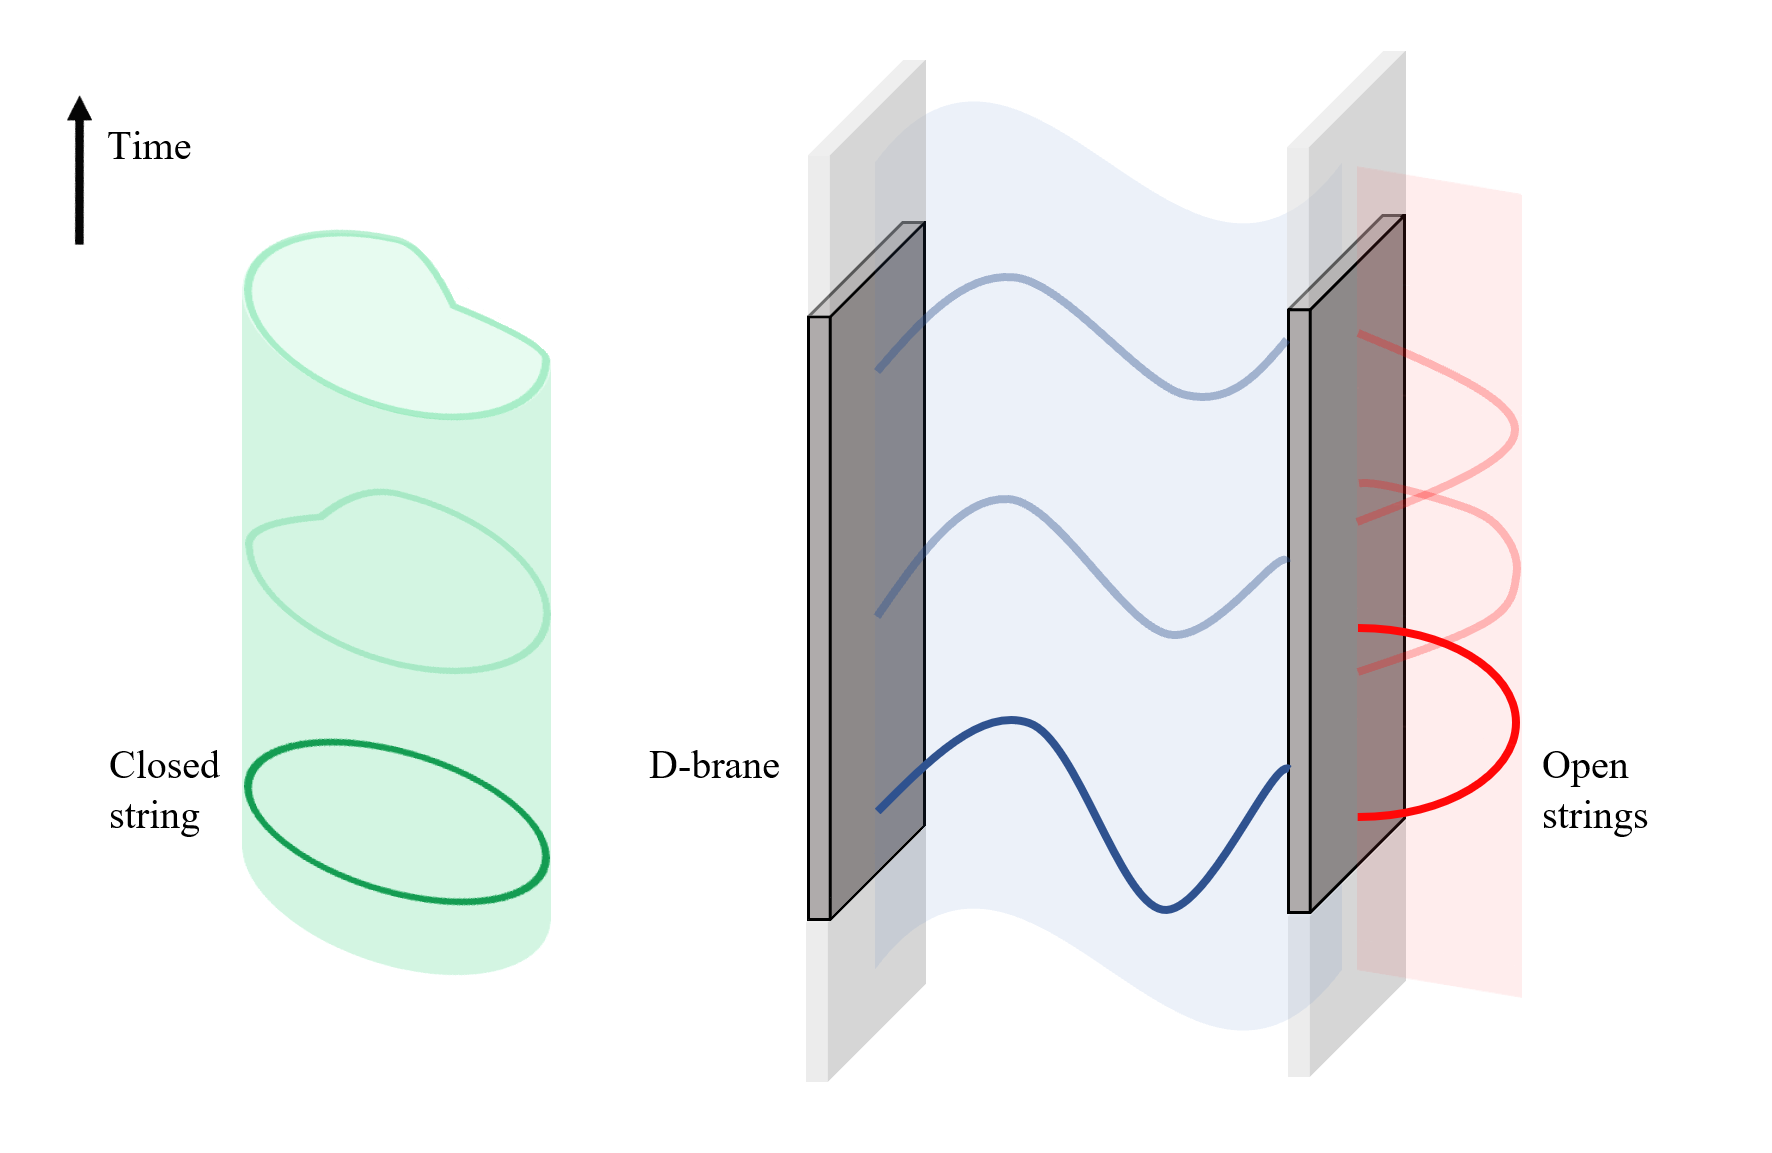
\includegraphics[width=0.55\linewidth]{fig14.png}
  \caption{一些可能的弦构型及其世界面。蓝色开弦的边界落在不同的 D-膜上，这应会令人想起第 5 章反复讨论的某个问题……\hfill（原书 p.111）}
  \label{fig:14}
\end{figure}

量子场论的公理早已提示，D-膜应当被组织成数学范畴（参看 \cite{ABCp09}）。具体说来，在 A-模型中相关对象（A-膜）是带平坦线丛的拉格朗日子流形，而在 B-模型中则是带有全纯向量丛的复子流形（B-膜）。第~\ref{sec:7.3} 节将考察这两种类型。
% [Tutor Note: 【背景】“A-膜是带平坦线丛的拉格朗日子流形”只是底线情形；一旦引入 B-场，平坦线丛须换成曲率为 iB|_L 的酉联络（见注 7.24），更一般地还要用扭复形与分级拉格朗日子流形来描述。]

1994 年，受开弦观点的推动，数学家 M. Kontsevich 登场。在苏黎世举行的国际数学家大会（ICM）上，他给出了镜像对称猜想的同调精细化（发表于 \cite{Kon94}）。他断言：给定满足 $c_1(X)=0$ 的 $2n$ 维辛流形 $(X,\omega)$ 与对偶的 $n$ 维复代数流形 $X^\dagger$，

\begin{quote}
“由 Fukaya 范畴 $\mathcal F(X)$（或某个适当扩大后的范畴）构造的导出范畴，等价于 $X^\dagger$ 上凝聚层的导出范畴”，
\end{quote}

从而在开弦理论与三角范畴之间画出一条平行线。这个论证有一半我们已经熟悉。于是，第~\ref{sec:7.3} 节的目标是尽可能合理地解释镜像那一侧究竟是什么，以及它如何嵌入猜想~\ref{con:7.26}——那是 Kontsevich 断言的一个（过于宽泛的）版本（\cite{Fuk02a} 中有概述）。最后我们还会提到 Strominger、Yau 与 Zaslow 三人的一个猜想：他们 1996 年的工作 \cite{SYZ96} 定性地说明了如何“具体地”构造一对镜像 Calabi–Yau 流形。
% [Tutor Note: 【含糊】Kontsevich 所说的“适当扩大后的范畴”，在本书语境中即对 $\mathcal F(X)$ 取分裂封闭扭复形所得的导出范畴 $\mathsf D^\pi(\mathcal F(X))$（也可换成 wrapped 版本），使得 Hom 集恰为 Floer 上同调；详见第 3.5、3.6 节与 \cite{Fuk02a} 第 2 章。]

在继续之前，我们要强调：弦论及其各分支（包括镜像对称）的严格数学表述，至今仍远未完成，这也是它们带有猜想性质的原因。除此之外，我们还选择一条更直接、更不分散的进路，把所有必要的要素只讨论到定义层面。除了常识之外，这样做还有两方面理由：一方面，我们希望给出一个自足的综述，使我们看清迄今发展出的理论嵌入“更大图景”的何处；另一方面，本章也充当一张试探性的路线图，为可能的后续工作指明方向。

\subsection{镜像对称}\label{sec:7.2}

镜像对称猜想的主角是 Calabi–Yau 流形。我们要给出的定义需要先在 Kähler 几何的领域里做几步准备。首先，我们绕开全纯图册，给出复流形的另一种刻画（证明在文献中很容易找到）。

\begin{Lem}[Newlander--Nirenberg 定理]\label{lem:7.1}
设 $M^n=(M,J)$ 是 $\mathbb C$ 上 $n$ 维近复流形。则它是复流形（如第 5.1 节所述），当且仅当其近复结构 $J\in\mathcal T^{1,1}(M)$ 使 Nijenhuis 张量
\[
N_J(X,Y):=[X,Y]+J\bigl([JX,Y]+[X,JY]\bigr)-[JX,JY]
\]
对所有 $X,Y\in\mathfrak X(M)$ 为零（此时称 $J$ 为 $M$ 的\textbf{可积复结构}）。
\end{Lem}

它与复流形通常定义的相容性，源于 Nijenhuis 张量 $N_J$ 正是（$J$-）全纯函数存在的障碍：所谓全纯函数，就是光滑函数 $f\in C^\infty(M,\mathbb C)$，满足 $(df)_x\circ J=i(df)_x$ 对一切 $x\in M$ 成立（其中 $df:=d(\operatorname{Re}(f))+i\,d(\operatorname{Im}(f))$；可与 $J$-全纯曲线的定义 5.7 对照）。
% [Tutor Note: 【易错】Newlander–Nirenberg 定理常被简写为“Nijenhuis 张量为零即复结构可积”。要点在于 J 必须属于 C^1 且 N_J 是 TM 值 2-形式，等式 N_J(X,Y)=0 的符号约定随 [JX,JY] 项的系数而异；本书采用 N_J = [X,Y] + J([JX,Y]+[X,JY]) − [JX,JY]。]

由于固定某个 Riemann 度量（它总是存在）之后，辛流形自然成为近复流形，我们有时用记号 $(M^{2n},J,\omega)$ 来强调它还带有复结构，其中维数 $2n$ 是就 $\mathbb R$ 而言的。

\begin{Rem}\label{rem:7.2}
下面是复微分几何的一些基本概念（更易消化的介绍见 \cite{Sil12} 第 14、15 章）。
\begin{itemize}
  \item $M^{2n}$ 上的近复结构 $J\in\mathcal T^{1,1}(M)\cong\Gamma(\operatorname{End}(TM))$ 可以延拓到复化切丛 $TM^{\mathbb C}:=TM\otimes\mathbb C$（其纤维为 $T_xM^{\mathbb C}=T_xM\otimes\mathbb C$）：只需令 $J(X\otimes z):=J(X)\otimes z$ 对一切 $X\in\mathfrak X(M)$、$z\in\mathbb C$ 成立。这样得到特征值为 $\pm i$ 的张量场 $J\in\mathcal T^{1,1}(TM^{\mathbb C})$（按定义如此），于是可把 $TM^{\mathbb C}$ 分解为两个特征子丛，即 $TM^{\mathbb C}=TM^{1,0}\oplus TM^{0,1}$。同样可构造复化余切丛 $T^*M^{\mathbb C}:=T^*M\otimes\mathbb C=T^*M^{1,0}\oplus T^*M^{0,1}$。
  \item 特别地，谈论 $(M,J)$ 上的复值形式才有意义：令 $\Lambda^{p,q}(T^*M^{\mathbb C}):=\Lambda^p(T^*M^{1,0})\wedge\Lambda^q(T^*M^{0,1})$，则\textbf{$(p,q)$-形式}是 $\Omega^{p,q}(M):=\Gamma(\Lambda^{p,q}(T^*M^{\mathbb C}))$ 的元素。然后定义
  \[
  \Omega^r(M):=\bigoplus_{p+q=r}\Omega^{p,q}(M)\;.
  \]
  若假定 $M$ 是复流形，则可把 $\Omega^{1,1}(M)$ 看成由 $dz\wedge d\bar z$ 局部张成的空间，其中 $z=x+iy\in C^\infty(M,\mathbb C)$ 是某个（全纯）坐标函数（从而 $dz\circ J=i\,dz=i\,dx-dy$）。
  \item 设 $\pi^{p,q}:\Lambda^r(T^*M^{\mathbb C}):=\bigoplus_{p+q=r}\Lambda^{p,q}(T^*M^{\mathbb C})\to\Lambda^{p,q}(T^*M^{\mathbb C})$ 表示到第 $(p,q)$ 个直和项的投影。于是（延拓后的）外微分算子 $d:\Omega^\bullet(M)\to\Omega^{\bullet+1}(M)$ 给出两个微分
  \[
  \partial_p:=\pi^{p+1,q}\circ d:\Omega^{p,q}(M)\to\Omega^{p+1,q}(M)\;,\qquad
  \bar\partial_q:=\pi^{p,q+1}\circ d:\Omega^{p,q}(M)\to\Omega^{p,q+1}(M)\;.
  \]
  对函数 $f\in C^\infty(M,\mathbb C)$，有 $d^0f=\partial^0f+\bar\partial^0f$，因此特别地，$f$ 全纯当且仅当 $\bar\partial^0f=0$。
  \item 事实上，在复流形 $M$ 上，对任意形式 $\nu\in\Omega^r(M)$ 都有 $d=\partial+\bar\partial$；又由 $0=d^2\nu=\partial^2\nu+(\partial\bar\partial+\bar\partial\partial)\nu+\bar\partial^2\nu$ 可推出：$\partial,\bar\partial$ 分别是上链复形 $\Omega^{\bullet,q}$ 与 $\Omega^{p,\bullet}$ 的（反交换的）上边缘算子。于是，对一切 $p,q\in\mathbb Z$，Dolbeault 上同调群
  \begin{equation}\label{eq:7.101}
  H^{p,q}_{Db}(M):=\frac{\ker(\bar\partial_q)}{\operatorname{im}(\bar\partial_{q-1})}
  \end{equation}
  都有良好定义。
  \item 进而，Dolbeault 定理给出同构
  \begin{equation}\label{eq:7.102}
  H^{p,q}_{Db}(M)\cong H^q(M;\Omega^{p,0}_M)\;,
  \end{equation}
  其中右端是与 $M$ 上 $(p,0)$-形式层 $\Omega^{p,0}_M$ 相伴的第 $q$ 个层上同调群（层上同调可参阅 \cite{Har77} 第 III 章）。这个结果可以看作 de Rham 定理的复类比。
\end{itemize}
\end{Rem}
% [Tutor Note: 【易错】第 (101) 式中 $\ker$ 与 $\operatorname{im}$ 都是无穷维空间，逐点定义的商只在复流形上才有意义；但当 $M$ 紧 Kähler 时，Hodge 定理保证 $H^{p,q}_{Db}(M)$ 有限维。另注意原书公式编号自 (101) 起，是全书连续编号，非按章重新计数。]
% [Tutor Note: 【含糊】第二条把 $\Lambda^{p,q}$ 写成 $\Lambda^p(T^*M^{1,0})\wedge\Lambda^q(T^*M^{0,1})$，严格说应是张量积 $\otimes$（两个向量丛一般不能作外积）；这是文献中常见的不严格写法，译文照印。]

\begin{Def}\label{def:7.3}
设 $M^n=(M,J)$ 是复流形，并配有 Riemann 度量 $h\in\Gamma(T^*M\otimes T^*M)$。若 $h(X,Y)=h(JX,JY)$ 对一切 $X,Y\in\mathfrak X(M)$ 成立（这意味着 $TM$ 上有一个光滑变化的正定 Hermitian 内积），则称 $h$ 为 \textbf{Hermitian 度量}，并称 $(M,J,h)$ 为 \textbf{Hermitian 流形}。注意这些数据确定了一个实 $(1,1)$-形式 $\kappa:=-\operatorname{Im}(h)\in\Omega^2(M)$，它满足 $\kappa(J\cdot,\cdot)=h(\cdot,\cdot)$。

此外，若还满足 $\nabla J=0$（其中 $\nabla$ 是 $h$ 的 Levi–Civita 联络），等价地若 $d\kappa=0$ 或 $\nabla\kappa=0$，则 $h$ 还是 \textbf{Kähler 度量}。此时称 $M=(M,J,h,\kappa)$ 为 \textbf{Kähler 流形}，称 $\kappa$ 为其 \textbf{Kähler 形式}；在局部坐标卡 $(U,(z_j)_{j=1}^n)$ 上它由
\begin{equation}\label{eq:7.103}
\kappa=\frac{i}{2}\sum_{j,k=1}^{n}G_{jk}\,dz_j\wedge d\bar z_k
\end{equation}
给出，其中 $(G_{jk}(x))$ 在一切 $x\in M$ 处都是正定 Hermitian 矩阵（\cite{Sil12} 第 16.1 节有证明）。
\end{Def}

从辛的观点看，Kähler 流形不过是带可积复结构 $J\in\mathcal J(M,\kappa)$ 的辛流形 $(M^{2n},\kappa)$，再配上一个相伴的 Kähler 度量 $\kappa^{\mathbb C}:=B-i\kappa$——它也叫\textbf{复化 Kähler 形式}——其中 $B=\operatorname{Re}(\kappa^{\mathbb C})$（即“B-场”）是由 $B(\cdot,\cdot):=\kappa(J\cdot,\cdot)$ 给出的 $M$ 上良好定义的 Riemann 度量（对照定义 5.6）。据此，我们略去冗余，直接把 Kähler 流形记作 $(M,J,\kappa^{\mathbb C})$，其中 $\kappa=-\operatorname{Im}(\kappa^{\mathbb C})$。
% [Tutor Note: 【易错】原书把 Re(κ^ℂ)=B 称作“B-场”，又说它是由 B(·,·):=κ(J·,·) 给出的 Riemann 度量。物理学惯例中的 B-场是一个闭 2-形式，复化 Kähler 形式通常写作 B+iω；此处 B 实际扮演度量的角色。另外本书 p.124 又写作 ρ=B+iκ（符号相反），见该处【勘误】。]

此外注意 $J\in\operatorname{Symp}(M,\kappa)$，这正是 $\kappa\in\Omega^2(M)$ 实际上是一个（$\partial/\bar\partial$-闭的）$(1,1)$-形式的原因，于是得到良好定义的 Dolbeault 上同调类 $\langle\kappa\rangle\in H^{1,1}_{Db}(M)$。

对紧 Kähler 流形，de Rham 上同调与 Dolbeault 上同调之间有直接联系：

\begin{Thm}[Hodge]\label{thm:7.4}
设 $M^n=(M,J,\kappa^{\mathbb C})$ 是紧 Kähler 流形。则有如下 \textbf{Hodge 分解}：
\[
H^r_{dR}(M;\mathbb C)\cong\bigoplus_{p+q=r}H^{p,q}_{Db}(M)\;,
\]
且 $H^{p,q}_{Db}(M)\cong\overline{H^{q,p}_{Db}(M)}$，所有 $H^{p,q}_{Db}(M)$ 都是有限维的。记 $b_r(M):=\dim\bigl(H^r_{dR}(M;\mathbb C)\bigr)$ 为 Betti 数，$h^{p,q}(M):=\dim\bigl(H^{p,q}_{Db}(M)\bigr)$ 为 $M$ 的 \textbf{Hodge 数}，于是有 $b_r(M)=\sum_{p+q=r}h^{p,q}(M)$ 以及 $h^{p,q}(M)=h^{q,p}(M)$。
\end{Thm}

Hodge 数的信息编码在所谓的 \textbf{Hodge 菱形}中：
\begin{equation}\label{eq:7.104}
\begin{array}{ccccccc}
& & & h^{n,n} & & & \\
& & h^{n,n-1} & & h^{n-1,n} & & \\
& h^{n,n-2} & & h^{n-1,n-1} & & h^{n-2,n} & \\
& \vdots & & \vdots & & \vdots & \\
& h^{2,0} & & h^{1,1} & & h^{0,2} & \\
& & h^{1,0} & & h^{0,1} & & \\
& & & h^{0,0} & & &
\end{array}
\end{equation}

中央一列由所有 $h^{k,k}(M)$ 组成，可以证明它们是正整数。底层 Dolbeault 上同调群的复共轭，对应于关于这条中央列的镜像；而关于菱形中心的对称则由 \textbf{Hodge $\ast$-算子}给出，它是映射 $\ast:\Lambda(T_xM)\to\Lambda(T_xM)$，
\[
\ast(v_1\wedge\dots\wedge v_k):=v_{k+1}\wedge\dots\wedge v_n
\qquad(\text{其中 }\ast(1)=v_1\wedge\dots\wedge v_n\text{，且 }\ast(v_1\wedge\dots\wedge v_n)=1)\;,
\]
它给出同构 $H^{p,q}_{Db}(M)\cong H^{n-p,n-q}_{Db}(M)$。
% [Tutor Note: 【含糊】这里 ∗ 的公式只对定向正交标架 (v_1,…,v_n) 成立；一般情形须先用度量把形式化为多重向量，再与体积形式缩并。原书用它说明 H^{p,q}_Db ≅ H^{n−p,n−q}_Db，与 Hodge 菱形的中心对称一致。]

还剩最后一点技术准备。

\begin{Def}\label{def:7.5}
设 $M=(M,g)$ 是配有 Levi–Civita 联络 $\nabla$ 的 Riemann 流形。$g$ 在 $x\in M$ 处的 \textbf{Riemann 和乐群}为
\[
\operatorname{Hol}_x(g):=\operatorname{Hol}^\nabla(x)=\{P_\gamma:T_xM\to T_xM\mid P_\gamma\text{ 为平行移动映射，}\gamma\text{ 是 }x\text{ 处的分段光滑闭路}\}\;,
\]
它可以看作子群\footnote{回忆：只要假定 $M$ 连通（我们默认如此），对任意 $x\in M$，在共轭意义下都有 $\operatorname{Hol}^\nabla(x)<\mathrm{GL}(n,\mathbb R)$。} $\operatorname{Hol}(g)<\mathrm O(n)$，如 \cite{GHJ03} 第 2.5 节所解释。特别地，给定 Kähler 流形 $(M^n,J,\kappa^{\mathbb C})$，可以证明 $\operatorname{Hol}(\kappa^{\mathbb C}):=\operatorname{Hol}(\operatorname{Re}(\kappa^{\mathbb C}))<\mathrm U(n)$（而 $\mathrm U(n)$ 本身又是 $\mathrm O(2n)$ 的子群；见 \cite{GHJ03} 第 4.2 节）。
\end{Def}
% [Tutor Note: 【背景】Berger 分类说，非对称空间上不可约的 Riemann 和乐群只有 SO(n)、U(n)、SU(n)、Sp(n)、Sp(n)·Sp(1)、G_2、Spin(7)。Kähler 流形对应 U(n)，Calabi–Yau 流形对应 SU(n)；记号 Hol(κ^ℂ) 中的 κ^ℂ 实际指其 Riemann 度量 Re(κ^ℂ)。]

现在终于可以定义 Calabi–Yau 流形了（参考文献为 \cite{GHJ03} 的定义 4.3）。

\begin{Def}\label{def:7.6}
\textbf{Calabi–Yau 流形} $X^n=(X,\varpi)$ 是指满足 $\operatorname{Hol}(\kappa^{\mathbb C})=\mathrm{SU}(n)$ 的紧 Kähler 流形 $(X,J,\kappa^{\mathbb C})$，并且配有全纯体积形式 $\varpi\in\Omega^{n,0}(X)$，满足
\[
\kappa^n/n!=(-1)^{n(n-1)/2}(i/2)^n\,\varpi\wedge\bar\varpi\;,
\]
我们称 $\varpi$ 为其 \textbf{Calabi–Yau 形式}。
\end{Def}
% [Tutor Note: 【易错】定义 7.6 的归一化 κ^n/n! = (−1)^{n(n−1)/2}(i/2)^n ϖ∧ϖ̄ 依赖 Kähler 形式与全纯体积形式的相位约定；把 ϖ 换成 e^{iθ}ϖ 时右端不变，这正是注 7.7 说 ϖ 仅在相差一个相位的意义下唯一的原因。]

\begin{Rem}[警告]\label{rem:7.7}
文献中对 Calabi–Yau 流形其实有好几种可能互不等价的定义。有些定义放弃紧性要求，或放弃整体和乐群等于 $\mathrm{SU}(n)$ 的要求；另一些则不提全纯体积形式 $\varpi$（事实上它在相差一个相位的意义下唯一确定；见 \cite{GHJ03} 引理 4.4）。许多作者只要求典范线丛 $K_X:=\Lambda^n(T^*X)\cong\Omega^{n,0}_X$ 平凡，即 $K_X\cong\mathcal O_X$（$X$ 上全纯函数层，见下文例~\ref{ex:7.12}），而 $\varpi$ 是它的一个常值截面。无论采用哪种定义，都可推出 $c_1(TX)=0$，且 $X$ 的 Ricci 曲率为零（这也是 Yau 所证明的 Calabi 猜想的推论）。
\end{Rem}

让我们把迄今见过的流形可能结构之间的蕴含关系链总结如下：

\begin{center}
\begin{minipage}{0.92\linewidth}\centering
\begin{tikzcd}[column sep=small, row sep=small]
  & & \text{complex} \arrow[dr, Rightarrow] & & \\
  \text{Calabi--Yau} \arrow[r, Rightarrow] & \text{Kähler} \arrow[ur, Rightarrow] \arrow[dr, Rightarrow] & & \text{almost complex} \arrow[r, Rightarrow] & \text{smooth even-dim.} \\
  & & \text{symplectic} \arrow[ur, Rightarrow] & &
\end{tikzcd}
\end{minipage}
\end{center}
% [Tutor Note: 【易错】小框图的箭头方向是“蕴含”：Calabi–Yau ⟹ Kähler，Kähler ⟹ 复且辛，复与辛各自 ⟹ 近复，近复 ⟹ 实偶维光滑流形。反向均不成立：例如 Hopf 曲面 S^3×S^1 是复流形，但 b_2=0，故不可能是辛流形；而并不是每个辛流形都能配上可积复结构。]

最后，下述陈述是镜像对称猜想的一个极其干瘪的版本。更完整的表述会动用 Gromov–Witten 理论与所谓的 Yukawa 耦合；读者可参阅 \cite{GHJ03} 第 15–17 章。
% [Tutor Note: 【背景】Gromov–Witten 不变量计数穿过给定同调类的 J-全纯曲线，是 A-模型的可观测量；它们通过量子上同调相乘（以三点不变量为结构常数）组织起来。Yukawa 耦合即三点函数 ⟨∂_i∂_j∂_k F⟩，其生成函数（prepotential）满足镜像对称预言的 Picard–Fuchs 方程。]

\begin{Con}[镜像对称猜想]\label{con:7.8}
给定 Calabi–Yau 流形 $X^n=(X,J,\kappa^{\mathbb C},\varpi)$，存在同维的“镜像” Calabi–Yau 流形 $X^\dagger=(X^\dagger,J^\dagger,\kappa^{\mathbb C\dagger},\varpi^\dagger)$，使得有自然同构
\begin{equation}\label{eq:7.105}
H^q(X,\Omega^p(T_X))\cong H^q(X^\dagger,\Omega^p_{X^\dagger})\;,\qquad
H^q(X^\dagger,\Omega^p(T_{X^\dagger}))\cong H^q(X,\Omega^p_X)\;.
\end{equation}
\end{Con}
% [Tutor Note: 【易错】式 (105) 中的 Ω^p(T_X) 指切丛的外幂 Λ^p T_X，而非 p-形式层 Ω^p_X；由与 ϖ 的缩并可得 Ω^p(T_X) ≅ Ω^{n−p,0}_X，因此 (105) 等价于 Hodge 数的“转 90°”对称。]

由于 $\Lambda^{p,0}(T_X^{\mathbb C})\to\Omega^{n-p,0}(X)$、$v_1\wedge\dots\wedge v_p\mapsto(i_{v_1}\circ\dots\circ i_{v_p})(\varpi)$ 是自然同构，故有 $\Omega^p(T_X)\cong\Omega^{n-p,0}_X$（类似地 $\Omega^p(T_{X^\dagger})\cong\Omega^{n-p,0}_{X^\dagger}$），于是可以把 \eqref{eq:7.105} 直接改写为 Dolbeault 上同调的语言：
\begin{equation}\label{eq:7.106}
H^{n-p,q}_{Db}(X)\cong H^{p,q}_{Db}(X^\dagger)\qquad\text{与}\qquad H^{n-p,q}_{Db}(X^\dagger)\cong H^{p,q}_{Db}(X)\;.
\end{equation}

特别地，定义模空间
\[
\mathcal M_{symp}(X):=\{\kappa\in\Omega^{1,1}(X)\mid\kappa\text{ 是 Kähler 形式}\}\;,\qquad
\mathcal M_{cplx}(X):=\{J\in\operatorname{Symp}(X,\kappa)\mid J\text{ 与 }\kappa\text{ 相容}\}/\operatorname{Diff}(X)\;,
\]
人们期待两个“镜像映射” $\mathcal M_{symp}(X)\to\mathcal M_{cplx}(X^\dagger)$ 与 $\mathcal M_{symp}(X^\dagger)\to\mathcal M_{cplx}(X)$，它们把 $H^{1,1}_{Db}(X)\cong H^1(X^\dagger,\Omega^{n-1}_{X^\dagger})\cong H^1(X^\dagger,T_{X^\dagger})$ 与反向的同构联系起来\footnote{用 \cite{Kon94} 中 Kontsevich 的话说，人们猜想：“用辛 [Calabi–Yau] 流形 $X$ 的 Gromov–Witten 不变量构造的纯 Hodge 结构的复变分，局部等价于 [$X^\dagger$ 上的] 代数几何变分”。}（群 $H^1(X,T_X)$ 支配 $(X,J)$ 的“形变”）。

从物理上说，最后这个陈述断言存在我们在第~\ref{sec:7.1} 节预告过的对应关系：“$(X,\kappa^{\mathbb C})$ 上的 A-模型 $\leftrightarrow$ $(X^\dagger,J^\dagger)$ 上的 B-模型”与“$(X,J)$ 上的 B-模型 $\leftrightarrow$ $(X^\dagger,\kappa^{\mathbb C\dagger})$ 上的 A-模型”。此外，该猜想还预言 $X$ 与 $X^\dagger$ 上的 SCFT（从而“它们的物理”）等价。

\begin{Rem}\label{rem:7.9}
对 Calabi–Yau 流形 $X^n$，Dolbeault 上同调上还有一族额外的对称性，来自 Hodge $\ast$-算子与 Calabi–Yau 形式的外积，即
\[
H^{p,0}_{Db}(X)\cong H^{n,n-p}_{Db}(X)\cong H^{n-p}(X,\mathcal O_X)\cong H^{0,n-p}_{Db}(X)\;,
\]
于是 $h^{p,0}(X)=h^{n-p,0}(X)$；这还不算定理~\ref{thm:7.4} 给出的 $h^{p,q}(X)=h^{q,p}(X)$ 与 $h^{p,q}(X)=h^{n-p,n-q}(X)$。

再注意 $H^{n,0}_{Db}(X)\cong H^0(X,\mathcal O_X)\cong\mathcal O_X(X)$（最后一个同构是层上同调的标准结果），于是 $h^{n,0}(X)=h^{0,n}(X)=1$。此外可以证明 $H^{0,0}_{Db}(X)\cong\mathbb C$，从而 $b_0(X)=h^{0,0}(X)=1$，且对 $0<k<n$ 有 $h^{k,0}(X)=0$（见 \cite{GHJ03} 命题 5.6）。
\end{Rem}

\begin{Ex}\label{ex:7.10}
让我们考察三维 Calabi–Yau 流形 $X$。由上一注可知 $h^{2,0}(X)=h^{0,2}(X)=0$，从而 $h^{1,3}(X)=h^{3,1}(X)=0$；又 $h^{1,0}(X)=h^{0,1}(X)=0$，从而 $h^{2,3}(X)=h^{3,2}(X)=0$；同时 $h^{3,3}(X)=h^{0,0}(X)=1$，$h^{3,0}(X)=h^{0,3}(X)=1$。因此（并利用 $h^{2,2}(X)=h^{1,1}(X)$ 与 $h^{2,1}(X)=h^{1,2}(X)$）得到如下退化 Hodge 菱形：
\begin{equation}\label{eq:7.107}
\begin{array}{ccccccc}
& & & 1 & & & \\
& & 0 & & 0 & & \\
& 0 & & h^{1,1} & & 0 & \\
1 & & h^{1,2} & & h^{1,2} & & 1 \\
& 0 & & h^{1,1} & & 0 & \\
& & 0 & & 0 & & \\
& & & 1 & & &
\end{array}
\end{equation}
\end{Ex}

于是，镜像对称猜想“不过”是说：存在对偶的三维 Calabi–Yau 流形 $X^\dagger$，其 Hodge 菱形由上述菱形绕其中心旋转 $90^\circ$ 得到。特别地，$h^{1,1}(X)=h^{1,2}(X^\dagger)$ 且 $h^{1,2}(X)=h^{1,1}(X^\dagger)$。

同理，在复维数 1 与 2 时得到 Hodge 菱形：
\begin{equation}\label{eq:7.108}
\begin{array}{c@{\qquad}c}
\begin{array}{ccc}
& 1 & \\
1 & & 1 \\
& 1 &
\end{array}
&
\begin{array}{ccccc}
& & 1 & & \\
& 0 & & 0 & \\
1 & & 20 & & 1 \\
& 0 & & 0 & \\
& & 1 & &
\end{array}
\end{array}
\end{equation}

确实，一维 Calabi–Yau 流形必然是某条复椭圆曲线 $\mathbb C/\Lambda$，其中 $\Lambda$ 是某个 $\mathbb Z^2$-格（特别地，它是例 6.30 研究过的辛二维环面 $\mathbb T^2$）。正如它们 Hodge 菱形的唯一性所暗示的，猜想~\ref{con:7.8} 断言这类流形自对偶，从而在它们上面给出辛结构与复结构之间的直接对应。

另一方面，二维 Calabi–Yau 流形是 K3 曲面，即满足 $h^{1,0}(X)=0$ 且典范丛平凡的紧复曲面；它们可以实现为 $\mathbb{CP}^3$ 中的代数曲面（例如射影簇 $X=V_p(x_0^4+x_1^4+x_2^4+x_3^4)$，即 Fermat 四次曲面）。反之，任何这样的曲面都可赋予 Calabi–Yau 结构。由于所有 K3 曲面彼此微分同胚，且 $b_2(X)=22$，我们得到上面画出的 Hodge 菱形。于是在维数 2 时，镜像对称转化为 K3 曲面之间的一种密切关系。
% [Tutor Note: 【易错】原文称 K3 曲面“可实现为 CP^3 中的代数曲面”。严格说只有四次曲面这一族 K3 能这样嵌入；一般 K3 是复二维紧流形且未必是代数的。译文照印原文措辞。]

然而，从 $n=3$ 起，这个猜想就获得了非平凡的风味，尤其因为目前尚不知道 Calabi–Yau 三维流形的拓扑族是否有限。非退化的五次三维流形——例如 Fermat 五次超曲面 $V_p(x_0^5+x_1^4+x_2^4+x_3^4+x_4^5)\subset\mathbb{CP}^4$ 这样的代数曲面——正是 \cite{CdGP91} 最初研究的对象；在那里，相应的 Hodge 菱形被证明满足 $h^{1,1}(X)=1=h^{1,2}(X^\dagger)$ 与 $h^{1,2}(X)=101=h^{1,1}(X^\dagger)$。\hfill$\blacklozenge$
% [Tutor Note: 【勘误】原文把 Fermat 五次超曲面写成 x_0^5+x_1^4+x_2^4+x_3^4+x_4^5，其中 x_1,x_2,x_3 的指数显然应为 5（五次超曲面是五次齐次多项式的零点集）；同句又把它称作“代数曲面（algebraic surfaces）”，但三维流形应称代数簇或三维流形。译文照印原文。]

\subsection{同调镜像对称}\label{sec:7.3}

我们先把代数几何中相关的定义收集起来。代数几何是同调镜像对称猜想的 B-侧所主导的理论（更详尽的叙述见 \cite{Har77} 或 \cite{Gat20}）。

\begin{Def}\label{def:7.11}
设 $X$ 是拓扑空间，$\mathsf C$ 是范畴。$X$ 上取值于 $\mathsf C$ 的\textbf{预层} $\mathcal F$ 由以下数据组成：
\begin{itemize}
  \item 对每个开子集 $U\subset X$ 有一个对象 $\mathcal F(U)\in\operatorname{obj}(\mathsf C)$，其元素 $s\in\mathcal F(U)$ 称为 $\mathcal F(U)$ 的\textbf{截面}；
  \item 对每一对开子集 $U\subset V\subset X$ 有\textbf{限制映射} $\rho_U^V\in\operatorname{Hom}_{\mathsf C}(\mathcal F(V),\mathcal F(U))$，
\end{itemize}
并满足：$\mathcal F(\varnothing)=\{0\}$；对一切开集 $U\subset X$ 有 $\rho_U^U=\operatorname{id}_{\mathcal F(U)}$；对一切三元组 $U\subset V\subset W\subset X$ 有 $\rho_U^V\circ\rho_V^W=\rho_U^W$。

若还满足“粘接性质”，则称预层 $\mathcal F$ 是 $X$ 上取值于 $\mathsf C$ 的\textbf{层}：对任意开子集 $U\subset X$ 及其开覆盖 $\{U_i\}_{i\in I}$，只要所有截面 $s_i\in\mathcal F(U_i)$ 彼此相容，即 $s_i|_{U_i\cap U_j}=s_j|_{U_i\cap U_j}$，就存在唯一的 $s\in\mathcal F(U)$ 使 $s|_{U_i}=s_i$ 对一切 $i\in I$ 成立。
\end{Def}

当 $\mathsf C=\mathsf{Sets}$，且特别地 $\mathcal F(U)\subset\operatorname{Hom}_{\mathsf{Sets}}(U,K)$ 对一切开子集 $U\subset X$ 成立时，$\mathcal F$ 是\textbf{$K$-值函数的层}（$K$ 为任意基域）。

（预）层的直和与限制在显然的指定下仍是（预）层。这里我们最感兴趣的是 $K=\mathbb C$ 与 $\mathsf C=\mathbb C\text{-}\mathsf{Alg}$（$\mathbb C$-代数范畴）的情形：

\begin{Ex}\label{ex:7.12}
设 $(X,J)$ 是复流形。通过指定
\[
U\mapsto\mathcal O_X(U):=\{f\in C^\infty(U,\mathbb C)\mid f\text{ 是 }J\text{-全纯的}\}
\]
（我们已在第~\ref{sec:7.2} 节开头定义过 $J$-全纯函数），得到 $X$ 上的\textbf{全纯函数层} $\mathcal O_X$。这是取值于 $\mathbb C\text{-}\mathsf{Alg}$ 的 $\mathbb C$-值函数层。\hfill$\blacklozenge$
\end{Ex}

\begin{Def}\label{def:7.13}
设 $X$ 是拓扑空间，其上配有取值于某范畴 $\mathsf C$ 的层 $\mathcal F,\mathcal G$。$X$ 上的\textbf{层态射} $\chi:\mathcal F\to\mathcal G$ 是一族映射 $\chi_U\in\operatorname{Hom}_{\mathsf C}(\mathcal F(U),\mathcal G(U))$（对所有开子集 $U\subset X$），使得对任意一对开子集 $U\subset V\subset X$ 都有
\[
\rho_U^V\circ\chi_V=\chi_U\circ\rho_U^V\in\operatorname{Hom}_{\mathsf C}(\mathcal F(V),\mathcal G(U))
\]
（其中 $\rho$ 同时表示 $\mathcal F$ 与 $\mathcal G$ 的限制映射）。

给定 $X$ 上另一个层态射 $\tilde\chi:\mathcal G\to\mathcal H$，我们按“逐点”方式定义 $\tilde\chi\circ\chi$：$(\tilde\chi\circ\chi)_U:=\tilde\chi_U\circ\chi_U\in\operatorname{Hom}_{\mathsf C}(\mathcal F(U),\mathcal H(U))$。这些运算给出良好定义的范畴 $\operatorname{Sh}(X;\mathsf C)$，即 $X$ 上取值于 $\mathsf C$ 的层的范畴。
\end{Def}

例如，取环范畴 $\mathsf C=\mathsf{Rings}$ 与 $\mathcal F\in\operatorname{Sh}(X;\mathsf{Rings})$，则 $X=(X,\mathcal F)$ 成为以 $\mathcal F$ 为结构层的\textbf{环空间}。

\begin{Ex}\label{ex:7.14}
设 $X$ 是复流形，$\mathcal O_X$ 是其全纯函数层。则 $(X,\mathcal O_X)$ 是良好定义的环空间（因为 $\mathbb C$-代数不过是富化的环）。\hfill$\blacklozenge$
\end{Ex}

\begin{center}
\fbox{\begin{minipage}{0.92\linewidth}
从此以后，谈到复流形 $X$ 时，我们都隐含地把它看作以 $\mathcal O_X$ 为结构层的环空间。
\end{minipage}}
\end{center}

\begin{Rem}\label{rem:7.15}
在代数几何中，人们通常研究代数上更丰富的\textbf{局部环空间}概念。设 $X$ 是拓扑空间，$\mathcal F$ 是 $X$ 上取值于 $\mathsf C$ 的预层。$\mathcal F$ 在 $x\in X$ 处的\textbf{茎}为
\[
\mathcal F_x:=\{(U,s)\mid x\in U,\ U\subset X\text{ 开},\ s\in\mathcal F(U)\}/\sim\;,
\]
其中 $(U,s)\sim(U',s')$ 当且仅当存在某个开子集 $V\subset U\cap U'$，使得 $x\in V$ 且 $s|_V=s'|_V$。我们把等价类 $[(U,s)]\in\mathcal F_x$ 称为 $\mathcal F$ 在 $x$ 处的\textbf{芽}。注意茎自动继承 $\mathsf C$ 中对象的结构。

于是，对 $\mathcal F\in\operatorname{Sh}(X;\mathsf{Rings})$，$(X,\mathcal F)$ 是局部环空间，当且仅当它是环空间并且每个茎 $\mathcal F_x$ 都是局部环（即只有一个极大理想）。
\end{Rem}

\begin{Def}\label{def:7.16}
设 $(X,\mathcal F)$ 是环空间。$X$ 上的 \textbf{$\mathcal F$-模层}（也简记为 $\mathcal F$-模）是 $X$ 上的层 $\mathcal Q$，使得对每个开子集 $V\subset X$，$\mathcal Q(V)$ 都是 $\mathcal F(V)$-模，并且相应的限制映射都是 $\mathcal F(V)$-模同态：
\[
\rho_U^V(s_1+s_2)=\rho_U^V(s_1)+\rho_U^V(s_2)\;,\qquad
\rho_U^V(\lambda\cdot s)=\rho_U^V(\lambda)\cdot\rho_U^V(s)\;,
\]
对一切开集 $U\subset V\subset X$ 与 $s,s_1,s_2\in\mathcal Q(V)$、$\lambda\in\mathcal F(V)$ 成立。
\end{Def}

给定 $X$ 上另一个 $\mathcal F$-模层 $\tilde{\mathcal Q}$，若每个环同态 $\chi_U:\mathcal Q(U)\to\tilde{\mathcal Q}(U)$ 都是 $\mathcal F(U)$-线性的，则称 $\chi:\mathcal Q\to\tilde{\mathcal Q}$ 是 \textbf{$\mathcal F$-模态射}。配以任意两个此类态射之间通常的复合，我们再次得到范畴结构；$\mathcal F$-模可以限制、可以直和，所得仍是其中的 $\mathcal F$-模。

现在，若还满足以下两条，则称 $\mathcal Q$ 是 $X$ 上的\textbf{凝聚 $\mathcal F$-模层}：
\begin{itemize}
  \item $\mathcal Q$ 是\textbf{有限生成}的，即对每个点 $x\in X$，存在开邻域 $U\subset X$ 与（限制后）层的满射 $\psi:\mathcal F|_U^{\oplus n}\to\mathcal Q|_U$，其中 $n\in\mathbb N$；
  \item 对一切开集 $U\subset X$、$n\in\mathbb N$ 以及 $\mathcal F$-模态射 $\chi:\mathcal F|_U^{\oplus n}\to\mathcal Q|_U$，$\chi$ 的核层 $\operatorname{Ker}(\chi)$ 都是有限生成的（该核层由 $V\mapsto\ker(\chi_V)$ 指定）。
\end{itemize}
此外，若第一条中的满射 $\psi$ 其实是层的同构（当且仅当每个 $\psi_V$ 都是双射），则称 $\mathcal Q$ 是\textbf{秩 $n$ 局部自由}的。

把 $X$ 上凝聚 $\mathcal F$-模层之间的态射定义为恰好其底层的 $\mathcal F$-模态射，便得到范畴 $\operatorname{Coh}(X,\mathcal F)$，即 $X$ 上凝聚 $\mathcal F$-模层的范畴。

\begin{Rem}\label{rem:7.17}
设 $X=(X,J)$ 是复流形。则秩 $k$ 的复向量丛 $\pi:E\to X$ 与秩 $k$ 的局部自由 $\mathcal O_X$-模层 $\mathcal E_E\cong\bigoplus_{i=1}^{k}\mathcal O_X$ 之间存在双射对应（例如见 \cite{Gat20} 注 14.18 或 \cite{Har77} 习题 5.18）。特别地，若 $k=1$，我们谈论的是\textbf{线丛}；因此我们将相应地互换记号：$E\leftrightarrow\mathcal E$ 或 $TL\leftrightarrow L$。

类似地，$X$ 上的全纯向量丛——即转移函数全纯的复向量丛——与 $X$ 上凝聚的 $\mathcal O_X$-模层是同一回事。相当粗略地说，我们把任何配有全纯向量丛 $\pi:E\to Y$ 的复子流形 $Y\subset X$ 称为由 $(X,J)$ 紧化的 B-模型的 \textbf{（B-）膜}。我们用 $\mathcal V(X,J)$ 表示 $X$ 上（稳定）B-膜的相应模空间。它在同调镜像对称猜想中扮演积极角色。
\end{Rem}
% [Tutor Note: 【含糊】这里把 B-膜“简化”为带全纯向量丛的复子流形，只是便于叙述的特例。导出范畴意义上的 B-膜还允许凝聚层的复形（乃至扭曲对象）；正是这些复形才与 Fukaya 一侧的扭复形一一对应，见猜想 7.26。]

\begin{Rem}\label{rem:7.18}
$\operatorname{Coh}(X,\mathcal F)$ 中任何凝聚层 $\mathcal Q$ 都自动是\textbf{拟凝聚}的，意思是存在 $X$ 的开覆盖 $\{U_i\}_{i\in I}$ 与正合列
\[
\bigoplus_{j\in I_i}\mathcal F|_{U_i}\xrightarrow{\ \psi_i\ }\bigoplus_{j\in J_i}\mathcal F|_{U_i}\xrightarrow{\ \chi_i\ }\mathcal Q|_{U_i}\to\{0\}
\]
（其中指标集 $I_i,J_i$ 可以无限），对一切 $i\in I$ 成立。于是注意，$\mathcal Q$ 局部地是 $\mathcal F$-模态射的余核：由正合性与层的同构定理，
\[
\mathcal Q|_{U_i}=\operatorname{im}(\chi_i)\cong\Bigl(\mathcal F|_{U_i}^{\oplus|J_i|}\Bigr)/\ker(\chi_i)=\operatorname{coker}(\psi_i)\;.
\]
的确，$\operatorname{Coh}(X,\mathcal F)$ 是阿贝尔范畴，因而含有态射的核与余核。
\end{Rem}

由上一注，我们可以正当地谈论有界导出范畴 $\mathsf D^{\mathrm b}(\operatorname{Coh}(X,\mathcal F))$。由于它恰是同调镜像猜想中 $\mathcal F(M)$ 的有界导出范畴的对应物，我们要更仔细地考察其结构。仿照定义 3.7 的精神，我们只给出概要，更严格的推导请读者参阅 \cite{GM03} 第 III.5–III.6 节。

\begin{Def}\label{def:7.19}
设 $\mathsf A,\mathsf B$ 是阿贝尔范畴，$F:\mathsf A\to\mathsf B$ 是加性左（相应地右）正合函子。若类 $\mathcal R\subset\mathsf A$ 满足：
\begin{itemize}
  \item $\mathcal R$ 对直和封闭；
  \item 对任意 $C^\bullet\in\operatorname{obj}(\operatorname{Kom}^+(\mathcal R))$——即 $\mathsf A$ 中任一有下界的无环复形（若在 $\operatorname{Kom}^-(\mathcal R)$ 中，则要求有上界）——$F(C^\bullet)$ 都是 $\mathsf B$ 中的无环复形；
  \item 对一切 $A\in\operatorname{obj}(\mathsf A)$，存在 $R\in\operatorname{obj}(\mathcal R)$ 与单射 $i\in\operatorname{Hom}_{\mathsf A}(A,R)$（此时称 $\mathcal R$ 有“足够多的内射对象”；反之，若存在满射 $p\in\operatorname{Hom}_{\mathsf A}(R,A)$，则称 $\mathcal R$ 有“足够多的投射对象”），
\end{itemize}
则称 $\mathcal R$ \textbf{适应于} $F$。

若这样的类存在，我们可以通过令 $RF(C^\bullet)^i:=F(C^i)$，定义从（适当局部化后的）$\operatorname{Kom}^+(\mathcal R)$ 到 $\mathsf D^+(\mathsf B)$（相应的有下界导出范畴）的函子 $RF$。再作一些额外选择，便可延拓为良好定义的三角函子 $RF:\mathsf D^+(\mathsf A)\to\mathsf D^+(\mathsf B)$，称为 $F$ 的\textbf{右导出函子}（若 $F$ 右正合，则得到左导出函子 $LF:\mathsf D^-(\mathsf A)\to\mathsf D^-(\mathsf B)$；当 $F$ 正合时它与 $RF$ 一致）。

我们令 $R^kF:=H^k(RF):\mathsf D^+(\mathsf A)\to\mathsf{Ab}$，即 $R^kF(C^\bullet)=H^k(F(C^\bullet))$（类似地 $L^kF:=H^k(LF):\mathsf D^-(\mathsf A)\to\mathsf{Ab}$）。于是由 $RF$ 的三角性，短正合列 $\{0\}\to A^\bullet\to B^\bullet\to C^\bullet\to\{0\}$ 诱导出长正合列
\[
\dots\to R^kF(A^\bullet)\to R^kF(B^\bullet)\to R^kF(C^\bullet)\to R^{k+1}F(A^\bullet)\to\dots
\]
（对 $LF$ 类似）。由这一构造也容易看出：当 $k<0$ 时 $R^kF=0$，且 $R^0F=F$（相应地，当 $k>0$ 时 $L^kF=0$，且 $L^0F=F$）。
\end{Def}

\begin{Def}\label{def:7.20}
设 $\mathsf A$ 是阿贝尔范畴，$A,B\in\operatorname{obj}(\mathsf A)$。把集中在次数 $0$ 的单对象复形记作 $A^\bullet:=(\dots\to\{0\}\to A\to\{0\}\to\dots)$ 与 $B^\bullet:=(\dots\to\{0\}\to B\to\{0\}\to\dots)$（而 $B^\bullet[k]:=B^{\bullet+k}$ 表示 $B$ 集中在次数 $-k$，一如往常）。则对 $k\in\mathbb Z$，定义第 $k$ 个 \textbf{Ext-阿贝尔群}
\begin{equation}\label{eq:7.109}
\operatorname{Ext}^k_{\mathsf A}(A,B):=\operatorname{Hom}_{\mathsf D^{\mathrm b}(\mathsf A)}(A^\bullet,B^\bullet[k])
\end{equation}
（$=\operatorname{Hom}_{\mathsf D^{\mathrm b}(\mathsf A)}(A^\bullet[l],B^\bullet[k+l])$，对任意 $l\in\mathbb Z$，这是对 $\mathsf D^{\mathrm b}(\mathsf A)$ 的平移函子作 $l$ 次作用的结果）。

由此得到函子 $\operatorname{Ext}^k_{\mathsf A}:\mathsf A^{opp}\times\mathsf A\to\mathsf{Ab}$，其中对任意 $A\in\operatorname{obj}(\mathsf A)$，$\operatorname{Ext}^k_{\mathsf A}(A,\square)$ 是共变的，$\operatorname{Ext}^k_{\mathsf A}(\square,A)$ 是反变的。于是，$\mathsf D^{\mathrm b}(\mathsf A)$ 中的复合 $A^\bullet\to B^\bullet[k]\to C^\bullet[k+l]$ 给出双线性积
\begin{equation}\label{eq:7.110}
\diamond:\operatorname{Ext}^k_{\mathsf A}(A,B)\otimes\operatorname{Ext}^l_{\mathsf A}(B,C)\to\operatorname{Ext}^{k+l}_{\mathsf A}(A,C)\;,
\end{equation}
即 \textbf{Yoneda 积}。
\end{Def}

\begin{Pro}\label{pro:7.21}
设 $\mathsf A$ 是阿贝尔范畴，$A,B\in\operatorname{obj}(\mathsf A)$ 固定。Ext-群具有以下性质：
\begin{itemize}
  \item $\mathsf A$ 中的短正合列 $\{0\}\to A\to A'\to A''\to\{0\}$ 与 $\{0\}\to B\to B'\to B''\to\{0\}$（看作 $\mathsf D^{\mathrm b}(\mathsf A)$ 中的区分三角形）分别诱导长正合列
  \[
  \dots\to\operatorname{Ext}^k_{\mathsf A}(A'',B)\to\operatorname{Ext}^k_{\mathsf A}(A',B)\to\operatorname{Ext}^k_{\mathsf A}(A,B)\to\operatorname{Ext}^{k+1}_{\mathsf A}(A'',B)\to\dots\;,
  \]
  \[
  \dots\to\operatorname{Ext}^k_{\mathsf A}(A,B)\to\operatorname{Ext}^k_{\mathsf A}(A,B')\to\operatorname{Ext}^k_{\mathsf A}(A,B'')\to\operatorname{Ext}^{k+1}_{\mathsf A}(A,B)\to\dots\;.
  \]
  \item 当 $k<0$ 时 $\operatorname{Ext}^k_{\mathsf A}(A,B)=\{0\}$，而 $\operatorname{Ext}^0_{\mathsf A}(A,B)=\operatorname{Hom}_{\mathsf A}(A,B)$。
  \item 若 $\mathsf A$ 有“足够多的内射对象”，则左正合函子 $\operatorname{Hom}_{\mathsf A}(A,\square):\mathsf A\to\mathsf{Ab}$ 有右导出函子 $R\operatorname{Hom}_{\mathsf A}(A,\square):\mathsf D^+(\mathsf A)\to\mathsf D^+(\mathsf{Ab})$，满足 $R^k\operatorname{Hom}_{\mathsf A}(A,\square)\cong\operatorname{Ext}^k_{\mathsf A}(A,\square)$（与~\eqref{eq:7.109} 相容）。
  \item 若 $\mathsf A$ 有“足够多的投射对象”，则左正合函子 $\operatorname{Hom}_{\mathsf A}(\square,B):\mathsf A^{opp}\to\mathsf{Ab}$ 有右导出函子 $R\operatorname{Hom}_{\mathsf A}(\square,B):\mathsf D^+(\mathsf A^{opp})\to\mathsf D^+(\mathsf{Ab})$，满足 $R^k\operatorname{Hom}_{\mathsf A}(\square,B)\cong\operatorname{Ext}^k_{\mathsf A}(\square,B)$（与~\eqref{eq:7.109} 相容）。
\end{itemize}
（注：最后两条与定义~\ref{def:7.19} 合起来蕴含前两条，事实上可以把它们用作 Ext-群的另一种定义。）
\end{Pro}
% [Tutor Note: 【背景】Ext 群是 Hom 的右导出函子：把相应变元换成内射消解（或投射消解）后再取上同调。第一条长正合列来自 Hom 函子作用于区分三角形所得的长正合列（见 \cite{GM03} 第 III 章），与定义 7.19 中 RF 的三角性一致。]

\begin{Def}\label{def:7.22}
考虑复流形 $X=(X,\mathcal O_X)$ 的阿贝尔范畴 $\operatorname{Coh}(X)$。则按定义 3.7 与 7.20，可以这样描述其\textbf{凝聚层的有界导出范畴} $\mathsf D^{\mathrm b}(\operatorname{Coh}(X))$：
\begin{itemize}
  \item $\operatorname{obj}\bigl(\mathsf D^{\mathrm b}(\operatorname{Coh}(X))\bigr)=\operatorname{obj}\bigl(\operatorname{Kom}^{\mathrm b}(\operatorname{Coh}(X))\bigr)$ 中的对象是 $X$ 上凝聚层的有界上链复形（的同伦类），例如 $Q^\bullet:=(\dots\to Q^{i-1}\to Q^i\to Q^{i+1}\to\dots)$，其中每个 $Q^i\in\operatorname{obj}(\operatorname{Coh}(X))$。
  \item 对单对象复形 $Q^\bullet,\tilde Q^\bullet\in\operatorname{obj}\bigl(\mathsf D^{\mathrm b}(\operatorname{Coh}(X))\bigr)$，Hom-群 $\operatorname{Hom}_{\mathsf D^{\mathrm b}(\operatorname{Coh}(X))}(Q^\bullet,\tilde Q^\bullet)$ 可通过等式~\eqref{eq:7.109} 与 Ext-群 $\operatorname{Ext}_{\operatorname{Coh}(X)}(Q,\tilde Q)$ 等同；这一等同可推广到 $X$ 上一般的凝聚层复形。
\end{itemize}
换个说法，按定义，$\mathsf D^{\mathrm b}(\operatorname{Coh}(X))$ 中的态射 $Q^\bullet\to\tilde Q^\bullet$ 是上链复形同伦范畴 $H(\operatorname{Coh}(X))$ 中的（等价类）\textbf{屋顶}：
\begin{equation}\label{eq:7.111}
\begin{tikzcd}[column sep=large, row sep=large]
& Q^\bullet \arrow[dl, "s"'] \arrow[dr, "t"] & \\
\mathcal U^\bullet & & \tilde Q^\bullet
\end{tikzcd}
\end{equation}
其中 $s\in S$（$S$ 是 $H(\operatorname{Coh}(X))$ 中全部拟同构构成的局部化类），$t\in\operatorname{Hom}_{H(\operatorname{Coh}(X))}(Q^\bullet,\tilde Q^\bullet)$。
\begin{itemize}
  \item 复合映射
  \[
  \operatorname{Hom}_{\mathsf D^{\mathrm b}(\operatorname{Coh}(X))}(Q_1^\bullet,Q_2^\bullet)\times\operatorname{Hom}_{\mathsf D^{\mathrm b}(\operatorname{Coh}(X))}(Q_0^\bullet,Q_1^\bullet)\to\operatorname{Hom}_{\mathsf D^{\mathrm b}(\operatorname{Coh}(X))}(Q_0^\bullet,Q_2^\bullet)
  \]
  是相应 Yoneda 积~\eqref{eq:7.110} 的延拓。
\end{itemize}
\end{Def}
% [Tutor Note: 【含糊】严格说 $\mathsf D^{\mathrm b}$ 的对象是复形本身，而不是“同伦类”；同伦类出现在态射的层面：$\operatorname{Kom}^{\mathrm b}$ 的 Hom 集模去链同伦后才成为导出范畴的 Hom 集。原书括号中的说法是简写，译文照印。]
% [Tutor Note: 【勘误】式 (111) 的“屋顶”图中，两支箭头从 $Q^\bullet$ 出发指向 $\mathcal U^\bullet$ 与 $\tilde Q^\bullet$；而导出范畴中表示态射 $Q^\bullet\to\tilde Q^\bullet$ 的标准屋顶应为 $Q^\bullet\xleftarrow{s}\mathcal U^\bullet\xrightarrow{t}\tilde Q^\bullet$（公共源为 $\mathcal U^\bullet$，$s$ 为拟同构）。原文所画方向与“$t\in\operatorname{Hom}(Q^\bullet,\tilde Q^\bullet)$”的声明倒是彼此一致，疑似作者笔误；译文照印原图方向，读者按标准定义理解即可。]

现在，定理 3.8 说明了 $\mathsf D^{\mathrm b}(\operatorname{Coh}(X))$ 如何被看作三角范畴。为了正确陈述同调镜像对称猜想，我们还必须把 Fukaya 范畴的定义也“富化”。

\begin{Def}\label{def:7.23}
设 $X$ 是复辛流形，$L\subset X$ 是拉格朗日子流形。$L$ 上的\textbf{局部系统}是\footnote{更一般地，拓扑空间上的（线性）局部系统是其上局部常值的层，且各茎具有有限维向量空间的结构。局部系统因而充当层上同调的系数。}复向量丛 $E\to L$，配有联络 $\nabla$，它平坦（从而 $E$ 上相应的分布可积），且对一切 $x\in L$，和乐群 $\operatorname{Hol}^\nabla(x)<\mathrm U(n)$ 都落在酉群中。若 $E$ 还配有相容的 Hermitian 度量 $h\in\Gamma(E^*\otimes E^*)$（定义~\ref{def:7.3} 的意义下），则称该局部系统是 \textbf{Hermitian} 的。我们简记
\[
\mathcal L:=(L,E,\nabla)\;.
\]
\end{Def}
% [Tutor Note: 【易错】平坦联络的和乐给出表示 $\pi_1(L)\to\mathrm{GL}(n,\mathbb C)$；要求和乐群落在 $\mathrm U(n)$ 内，即要求该表示是酉表示。按 Riemann–Hilbert 对应，秩 $n$ 的平坦复向量丛等价于 $\pi_1(L)$ 的 $n$ 维复表示，而对应的局部常值层就是通常所说的局部系统。在 A-模型中若 B-场非零，则 A-膜的联络曲率不再是零而是 $iB|_L$，见注 7.24。]

\begin{Rem}\label{rem:7.24}
设 $X=(X,J,\kappa^{\mathbb C},\varpi)$ 是 Calabi–Yau 流形，复化 Kähler 形式为 $\kappa^{\mathbb C}=B-i\kappa$。在由 $(X,\kappa^{\mathbb C})$ 紧化的 A-模型的语境中，若 $\nabla$ 的曲率满足 $R^\nabla=iB|_L$（其中 $E$ 可以是平坦的 $\mathrm U(1)$-线丛），则称 $\mathcal L=(L,E,\nabla)$ 为 \textbf{（A-）膜}。

进而，若 $L_0,L_1$ 通过某个 $\phi\in\operatorname{Ham}(X,\kappa)$（对照定义 5.5）哈密顿同痕，使得 $\phi^*E_1\cong E_0$，并且存在 $L_0\times[0,1]$ 上的联络 $\tilde\nabla$ 满足 $R^{\tilde\nabla}=i\phi^*(B)$ 与 $\tilde\nabla|_{L_0\times\{t\}}=\phi_t^*(\nabla_t)$（$t=0,1$），则称两个膜 $\mathcal L_0=(L_0,E_0,\nabla_0)$ 与 $\mathcal L_1=(L_1,E_1,\nabla_1)$ \textbf{哈密顿等价}。我们把诱导的商集记作 $\mathcal Lag(X,\kappa^{\mathbb C})$。

再做些工作（见 \cite{Fuk02a} 第 2 章），便可以把 $\mathcal Lag(X,\kappa^{\mathbb C})$ 看作由 $(X,\kappa^{\mathbb C})$ 紧化的 A-模型在 $X$ 上（稳定）A-膜的模空间。值得注意的是，它带有复结构，其切空间为 $T_{\mathcal L}\mathcal Lag(X,\kappa^{\mathbb C})\cong H^1(L;\Lambda_{\mathbb C})$。
\end{Rem}

\begin{Def}\label{def:7.25}
设 $X=(X,\omega)$ 是满足 $2c_1(TX)=0$ 的复辛流形。$X$ 的\textbf{“富化”Fukaya 范畴} $\widetilde{\mathcal F}(X)$ 具有以下结构：
\begin{itemize}
  \item 对象是（经过适当装饰的）紧拉格朗日子流形 $\mathcal L=(L,E,\nabla)$，配有 Hermitian 局部系统。
  \item $\mathcal L_0,\mathcal L_1\in\operatorname{obj}(\widetilde{\mathcal F}(X))$ 的态射空间为
  \begin{equation}\label{eq:7.112}
  \hom_{\widetilde{\mathcal F}(X)}(\mathcal L_0,\mathcal L_1)=CF(\mathcal L_0,\mathcal L_1):=\bigoplus_{p\in\mathcal X(L_0,L_1)}\operatorname{Hom}(E_0|_p,E_1|_p)\otimes\Lambda_{\mathbb C}\;.
  \end{equation}
  \item 给定 $\mathcal L_0,\dots,\mathcal L_d\in\operatorname{obj}(\widetilde{\mathcal F}(X))$，使得 $L_d\cap L_0=\{q:=p_{d+1}\equiv p_0\}$ 且 $L_i\cap L_{i+1}=\{p_{i+1}\}$（$i=0,\dots,d-1$），沿界定 (81) 的任一解 $u\in\mathcal M(p_1,\dots,p_d,q;[u],J,H)$ 的拉格朗日弧作平行移动（关于相应的联络 $\nabla_i$），得到线性同构 $\mathbb P_{\gamma_i}\in\operatorname{Hom}(E_i|_{p_i},E_i|_{p_{i+1}})$。于是，我们定义复合映射 $\mu^d\equiv\mu^d_{\widetilde{\mathcal F}(X)}$ 为下式的 $\Lambda_K$-线性延拓：
  \begin{equation}\label{eq:7.113}
  \mu^d(f_d,\dots,f_1):=\sum_{\substack{q\in\mathcal X(L_0,L_d)\\ [u]:\ \operatorname{ind}([u])=2-d}}\bigl(\#\mathcal M(p_1,\dots,p_d,q;[u],J,H)\bigr)\,T^{\omega([u])}\,\eta_{[u],f_d,\dots,f_1}\;,
  \end{equation}
  其中 $f_i\in\hom_{\widetilde{\mathcal F}(X)}(\mathcal L_{i-1},\mathcal L_i)$，且 $\eta_{[u],f_d,\dots,f_1}:=\mathbb P_{\gamma_d}\circ f_d\circ\dots\circ\mathbb P_{\gamma_1}\circ f_1\circ\mathbb P_{\gamma_0}\in\operatorname{Hom}(E_0|_q,E_d|_q)$。
\end{itemize}
\end{Def}
% [Tutor Note: 【背景】式 (112) 与 (113) 是 Floer 理论的“装饰”版本：$\Lambda_{\mathbb C}$ 是 Novikov 域，变量 $T$ 记录圆盘面积 $\omega([u])$；$\operatorname{ind}([u])$ 是圆盘的 Maslov 指标；$\mathcal M(\dots)$ 是以 $p_1,\dots,p_d,q$ 为边界穿孔的 $J$-全纯圆盘模空间，$\#\mathcal M$ 表示带符号计数。(113) 正是 $A_\infty$-关系在拉格朗日 Floer 理论中的来源。]
% [Tutor Note: 【易错】$\mathcal X(L_0,L_1)$ 表示两条拉格朗日子流形的横截交点集；只有当 $L_0,L_1$ 已作 Hamiltonian 扰动并处于一般位置时它才是有限集，$\mu^d$ 的求和才收敛（在 Novikov 域中按能量从上到下有限）。]

取上同调，便得到“富化”的 \textbf{Fukaya–Donaldson 范畴} $H(\widetilde{\mathcal F}(X))$，其 Hom-群是由上链复形 $(CF(\mathcal L_0,\mathcal L_1),\mu^1)$ 得来的 Floer 上同调环 $\operatorname{Hom}_{H(\widetilde{\mathcal F}(X))}(\mathcal L_0,\mathcal L_1)=HF(\mathcal L_0,\mathcal L_1)$。

这一变体所依托的 Floer 理论细节，我们不在此讨论（\cite{Fuk02a} 第 2 章有部分分析），但我们会保留 Floer 复形与上同调的记号。我们只再指出：wrapped Fukaya 范畴的定义也可以适当改动，以契合这个富化版本。

如我们现在所知，径直取上同调得到 $H(\widetilde{\mathcal F}(X))$ 会丢掉太多信息。我们转而考虑 $\widetilde{\mathcal F}(X)$ 的\textbf{分裂封闭导出范畴}
\[
\mathsf D^\pi(\widetilde{\mathcal F}(X))=H^0\bigl(\Pi(\operatorname{Tw}\widetilde{\mathcal F}(X))\bigr)\;,
\]
它保留了三角性与分裂直和项。关于后者结构的明确陈述，我们请读者复习第 3.5 与 3.6 节。
% [Tutor Note: 【背景】$\operatorname{Tw}$ 取扭复形，$\Pi$ 取幂等完备化（分裂封闭），$H^0$ 取第零次上同调；三步合起来把 $A_\infty$-范畴变成三角范畴。原书上标写的是 $\mathsf D^\pi$，这只是分裂封闭导出范畴的记号，不要与基本群 $\pi_1$ 混淆。]

猜想~\ref{con:7.8} 的同调版本可以陈述如下（参看 \cite{Fuk02a} 第 2 章）。

\begin{Con}[同调镜像对称猜想]\label{con:7.26}
给定 Calabi–Yau 流形 $X^n=(X,J,\kappa^{\mathbb C},\varpi)$，存在同维的“镜像” Calabi–Yau 流形 $X^\dagger=(X^\dagger,J^\dagger,\kappa^{\mathbb C\dagger},\varpi^\dagger)$，以及三角范畴的等价
\begin{equation}\label{eq:7.114}
\mathsf D^\pi(\widetilde{\mathcal F}(X))\cong\mathsf D^{\mathrm b}(\operatorname{Coh}(X^\dagger))
\qquad\text{与}\qquad
\mathsf D^\pi(\widetilde{\mathcal F}(X^\dagger))\cong\mathsf D^{\mathrm b}(\operatorname{Coh}(X))\;.
\end{equation}
\end{Con}

因此，以下对应关系成立：
\begin{itemize}
  \item （由拉格朗日子流形分裂封闭地生成的扭复形）$L\in\operatorname{obj}\bigl(\mathsf D^\pi(\widetilde{\mathcal F}(X))\bigr)$ 对应于凝聚层的有界上链复形（的同伦类）$E^\dagger\in\operatorname{obj}\bigl(\mathsf D^{\mathrm b}(\operatorname{Coh}(X^\dagger))\bigr)$；镜像地，$L^\dagger\in\operatorname{obj}\bigl(\mathsf D^\pi(\widetilde{\mathcal F}(X^\dagger))\bigr)$ 对应于 $E\in\operatorname{obj}\bigl(\mathsf D^{\mathrm b}(\operatorname{Coh}(X))\bigr)$。
  \item Hom-群同构于 Ext-群：
  \[
  \operatorname{Hom}_{\mathsf D^\pi(\widetilde{\mathcal F}(X))}(L_0,L_1)\equiv HF(L_0,L_1)\cong\operatorname{Ext}(E_0^\dagger,E_1^\dagger)\equiv\operatorname{Ext}_{\operatorname{Coh}(X^\dagger)}(E_0^\dagger,E_1^\dagger)\;,
  \]
  \[
  \operatorname{Hom}_{\mathsf D^\pi(\widetilde{\mathcal F}(X^\dagger))}(L_0^\dagger,L_1^\dagger)\equiv HF(L_0^\dagger,L_1^\dagger)\cong\operatorname{Ext}(E_0,E_1)\equiv\operatorname{Ext}_{\operatorname{Coh}(X)}(E_0,E_1)\;.
  \]
  值得注意的是，$\operatorname{Ext}^k(E^\dagger,E^\dagger)\cong H^k(L;\Lambda_{\mathbb C})$（由命题 5.43 的一个变体），反向也成立。
  \item 在这些同构下，Floer 积
  \[
  \langle\mu^2\rangle:HF(L_1,L_2)\otimes HF(L_0,L_1)\to HF(L_0,L_2)
  \quad\text{与}\quad
  \langle\mu^2\rangle:HF(L_1^\dagger,L_2^\dagger)\otimes HF(L_0^\dagger,L_1^\dagger)\to HF(L_0^\dagger,L_2^\dagger)
  \]
  分别化为 Yoneda 积
  \[
  \diamond:\operatorname{Ext}(E_1^\dagger,E_2^\dagger)\otimes\operatorname{Ext}(E_0^\dagger,E_1^\dagger)\to\operatorname{Ext}(E_0^\dagger,E_2^\dagger)
  \quad\text{与}\quad
  \diamond:\operatorname{Ext}(E_1,E_2)\otimes\operatorname{Ext}(E_0,E_1)\to\operatorname{Ext}(E_0,E_2)\;.
  \]
\end{itemize}

从物理上说，我们得到由 $(X,\kappa^{\mathbb C})$ 紧化的 A-模型在 $X$ 上（稳定）A-膜 $\mathcal L$ 的模空间 $\mathcal Lag(X,\kappa^{\mathbb C})$ 与由 $(X^\dagger,J^\dagger)$ 紧化的 B-模型在 $X^\dagger$ 上（稳定）B-膜 $\mathcal E^\dagger$ 的模空间 $\mathcal V(X^\dagger,J^\dagger)$ 之间的双射对应\footnote{更精确地说，存在 $\mathcal V(X^\dagger,J^\dagger)$ 中 $\mathcal E^\dagger$ 的一个邻域 $\mathcal U$ 与一个概形 $Y\subset\operatorname{Ext}^1(\mathcal E^\dagger,\mathcal E^\dagger)\cong H^1(L;\Lambda_{\mathbb C})\cong T_{\mathcal L}\mathcal Lag(X,\kappa^{\mathbb C})$ 之间的同构。}（对照注~\ref{rem:7.17} 与注~\ref{rem:7.24}），以及镜像的对应。

\begin{Rem}\label{rem:7.27}
猜想~\ref{con:7.26} 是 \cite{Kon94} 中 Kontsevich 所给版本的膨胀，膨胀到过于一般而未必成立的程度。例如，对象之间的双射并不成立，因为 $\operatorname{obj}\bigl(\mathsf D^{\mathrm b}(\operatorname{Coh}(X^\dagger))\bigr)$ 通常比 $\operatorname{obj}\bigl(\mathsf D^\pi(\widetilde{\mathcal F}(X))\bigr)$ 大。此外，$\mathcal Lag(X,\kappa^{\mathbb C})$ 先验地无阻碍，而 $\mathcal V(X^\dagger,J^\dagger)$ 却可能仍带阻碍\footnote{一个可能的解决办法由 Fukaya 在 \cite{Fuk02a} 猜想 3.21 中提出，即借助弯曲 $A_\infty$-范畴中的界定链（bounding chains，如注 6.14 所述）。否则，$HF(\mathcal L,\mathcal L)$ 与 $H(L;\Lambda_{\mathbb C})$ 一般只通过一个谱序列相联系。}，从而危及态射群之间以及复合映射之间的对应。

因此，人们有时会舍弃一部分 Calabi–Yau 装饰，只保留 $X=(X,\kappa)$ 上的辛结构与其镜像 $X^\dagger=(X^\dagger,J^\dagger)$ 上的复结构；这一取舍也受制于这样一个事实——据作者所知，迄今还没有展示对应 $(X,J)\leftrightarrow(X^\dagger,\kappa^\dagger)$ 的例子。

无论如何我们都要强调：镜像流形的存在性与唯一性都没有保证——毕竟我们谈的是一个猜想。
\end{Rem}
% [Tutor Note: 【含糊】原文说 $\mathcal V(X^\dagger,J^\dagger)$ “might be still”，字面费解；由其脚注（$HF(L,L)$ 与 $H(L;\Lambda_{\mathbb C})$ 只通过谱序列相联系）判断，这里应读作“仍可能带阻碍（obstructed）”。译文按此理解处理，原文措辞照印。]

\begin{Ex}\label{ex:7.28}
我们简要列举几个例子，并指出相关文献\footnote{更详尽的已验证情形清单很容易在网上找到，例如 \url{https://ncatlab.org/nlab/show/mirror+symmetry}。}。
\begin{itemize}
  \item 第一个非平凡情形是复椭圆曲线（其镜像对称我们已在例~\ref{ex:7.10} 讨论过），由 Polishchuk 与 Zaslow 在 \cite{PZ00} 中证明。这里的优点是：涉及扭复形的 $\mathsf D^\pi(\widetilde{\mathcal F}(X))$ 的构造可以绕开。作者们改为直接处理富化的 Donaldson–Fukaya 范畴 $\mathcal F^0(X):=H(\widetilde{\mathcal F}(X))$，并证明
  \begin{equation}\label{eq:7.115}
  \mathcal F^0(E^\rho)\cong\mathsf D^{\mathrm b}(\operatorname{Coh}(E_\tau))\;,
  \end{equation}
  其中 $X:=E^\rho$ 是配有复化 Kähler 形式 $\rho=B+i\kappa$ 的辛二维环面 $\mathbb T^2$（回忆例 6.30），$X^\dagger:=E_\tau$ 是椭圆曲线 $\mathbb C/\Lambda$，$\Lambda:=\langle1,\tau\rangle$（$\operatorname{Im}(\tau)>0$）。对偶关系翻译为 $\rho\leftrightarrow\tau$。
% [Tutor Note: 【勘误】此处写作 $\rho=B+i\kappa$，而定义 7.3 之后、注 7.24 与猜想 7.8 中复化 Kähler 形式都写作 $\kappa^{\mathbb C}=B-i\kappa$，符号相反。译文照印原文，读者注意本书内部约定不一致。]
  \item 在 \cite{PZ00} 中，椭圆曲线是在一般基域 $K$ 上处理的，而二维环面的辛侧（不失一般性）在 $\mathbb C$ 上讨论。Abouzaid 与 Smith 把分析专门化到 $K=\Lambda_{\mathbb R}$，证明了 \cite{AS09} 定理 6.4：
  \begin{equation}\label{eq:7.116}
  \mathsf D^\pi(\mathcal F(\mathbb T^2))\cong\mathsf D^{\mathrm b}(\operatorname{Coh}(E_A))\;,
  \end{equation}
  其中 $\mathbb T^2$ 配有标准面积形式 $\kappa=A\,d\theta_1\wedge d\theta_2$，而 $E_A:=\Lambda_{\mathbb R}^*/\langle T_A\rangle$ 是 Tate 椭圆曲线（的解析化），它由其坐标环 $\Lambda_{\mathbb R}[x,y]/\{y^2+xy=x^3+a_4(T)x+a_6(T)\}$ 代数地定义（形式变量 $T\in\Lambda_{\mathbb R}$ 的无穷级数 $a_4,a_6$ 的定义见 \cite{AS09} 定义 6.3）。此结果后来被用来证明 $QH(\mathbb T^2;\Lambda_{\mathbb R})\cong HH(\mathcal F^2)$；参看注 6.18。
% [Tutor Note: 【含糊】原文此处写作 $HH(\mathcal F^2)$，其中上标 2 的含义未在正文交代；按注 6.18 的语境，应为二维环面 $\mathbb T^2$ 的 Fukaya 范畴的 Hochschild 上同调，即 $HH(\mathcal F(\mathbb T^2))$。译文照印原记号。]
  \item 在 \cite{AS09} 中，Abouzaid 与 Smith 随后转向其主要目标，即关于四维环面\footnote{与例 6.30 和命题 6.31 所提示的分析类似，$\mathcal F(\mathbb T^4)$ 被四个二维环面分裂生成，这些环面由经线与纬线的两两乘积得到。} $\mathbb T^4=\mathbb R^4/\mathbb Z^4$ 在 $\Lambda_{\mathbb R}$ 上的一个等价：
  \begin{equation}\label{eq:7.117}
  \mathsf D^\pi(\mathcal F(\mathbb T^4))\cong\mathsf D^{\mathrm b}(\operatorname{Coh}(E_A\times E_A))\;,
  \end{equation}
  它可推广为：对任意 $k\in\mathbb Z$，有 $\mathsf D^\pi(\mathcal F(\mathbb T^{2k}))\cong\mathsf D^{\mathrm b}(\operatorname{Coh}(E_A^k))$（并为 Fukaya 范畴的一个无阻碍版本）。
  \item 在 \cite{Sei13} 中，Seidel 在 $\Lambda_{\mathbb Q}$ 上对任意四次曲面 $X_0\subset\mathbb{CP}^3$ 证明了该猜想（四次曲面即四元四次齐次多项式的零点轨迹给出的射影簇）。
  \item 此外，同调镜像对称猜想的若干部分分别由 Fukaya 对阿贝尔簇（\cite{Fuk00}）、由 Kontsevich 与 Soibelman 对环面纤维化（\cite{KS01}）作了讨论。
  \item 也有一些推广到非 Calabi–Yau 流形的情形，例如亏格 $g\ge 2$ 的曲面（见 \cite{Sei11}），或镜像为 Landau–Ginzburg 模型的 Fano 簇（\cite{Aur07}）。\hfill$\blacklozenge$
\end{itemize}
\end{Ex}

现在读者可能会合理地发问：“实际上怎样才能构造出 Calabi–Yau 流形的镜像对呢？”答案由 Strominger、Yau 与 Zaslow 的工作 \cite{SYZ96} 给出，它发表于 Kontsevich 的猜想之后两年。其动机来自下述观察。

\begin{Rem}\label{rem:7.29}
镜像 Calabi–Yau 流形 $X^\dagger$ 中的点 $p\in X^\dagger$ 与\textbf{摩天层} $\mathcal O_p\in\operatorname{obj}(\operatorname{Coh}(X^\dagger))\subset\operatorname{obj}\bigl(\mathsf D^{\mathrm b}(\operatorname{Coh}(X^\dagger))\bigr)$ 一一对应；后者由以下指定定义：
\begin{equation}\label{eq:7.118}
U\subset X^\dagger\text{ 开}\ \longmapsto\ \mathcal O_p(U):=
\begin{cases}
\mathbb C & \text{若 } p\in U\;,\\
\{0\} & \text{否则}\;.
\end{cases}
\end{equation}
（摩天层的主要特征，尤其在代数几何领域中的用法，见 \cite{Gat20} 第 13、14 章。）因此，我们可以把 $X^\dagger$ 等同于 $X^\dagger$ 上摩天层的模空间；按猜想~\ref{con:7.26}，后者又应对应于 $\mathsf D^\pi(\widetilde{\mathcal F}(X))$ 中某类对象 $L_p$ 的模空间。

现在，层上同调中的一个练习可证明 $\operatorname{Ext}^k_{\operatorname{Coh}(X^\dagger)}(\mathcal O_p,\mathcal O_p)\cong\Lambda^kT_pX^\dagger$（例如见 \cite{Aur09} 第 16 讲）。又因 $\operatorname{Ext}(\mathcal O_p,\mathcal O_p)\cong H(\mathbb T^n;\mathbb C)\cong HF(\mathbb T^n,\mathbb T^n)$（作为分次向量空间，再次利用命题 5.43），我们不禁要说：这些 $L_p$ 不是别的，正是\textbf{拉格朗日环面} $\mathbb T^n$，即微分同胚于标准环面 $\mathbb T^n\subset\mathbb R^{2n}\cong\mathbb C^n$ 的 $2n$ 维辛流形。
\end{Rem}
% [Tutor Note: 【易错】此处的关键计算是：光滑点处 $\operatorname{Ext}^\bullet(\mathcal O_p,\mathcal O_p)$ 是外代数 $\Lambda^\bullet T_pX^\dagger$，它在镜像一侧与 $H^\bullet(\mathbb T^n)$ 同构。这提示镜像对象应具有 $n$ 维环面的 Floer 上同调；点本身不是 Fukaya 范畴的对象（那里对象是 $n$ 维拉格朗日子流形），故不能取“点”作镜像。]

这已经足够接近我们感兴趣的对象了。我们只需要下面几个概念。

\begin{Def}\label{def:7.30}
设 $X=(X,J,\kappa^{\mathbb C})$ 是 Kähler 流形，$\varpi\in\Omega^{n,0}(X)$ 是全纯体积形式。若 $|\varpi|_\kappa:=\sqrt{|\kappa(\varpi,\bar\varpi)|}=g\in C^\infty(X,\mathbb R_{>0})$ 且 $\varpi\wedge\bar\varpi=\operatorname{const}(n)\,g^2\kappa^n$，则称 $X$ 为\textbf{几乎 Calabi–Yau}流形。
% [Tutor Note: 【含糊】此处 $\kappa(\varpi,\bar\varpi)$ 用 Kähler 形式 $\kappa$ 的记号表示由其诱导的 Hermitian 内积，而非 $2$-形式的求值；$|\varpi|_\kappa$ 就是全纯体积形式关于该度量的点态范数。]
\end{Def}

$X$ 中的拉格朗日环面 $T\subset X$ 满足 $\varpi|_T=e^{i\phi}g\cdot\operatorname{vol}_\kappa|_T$，其中相位函数 $e^{i\phi}:T\to S^1$（回忆定义 5.21）。若 $e^{i\phi}$ 实际上是常数，则称 $T$ 为\textbf{特殊}的（这最终蕴含 $\operatorname{Im}(\varpi|_T)=0$，即一般拉格朗日子流形为特殊拉格朗日的条件）。

最后，我们陈述以 Strominger、Yau 与 Zaslow 命名的“几何”镜像对称猜想。它建立在注~\ref{rem:7.29} 的直觉之上：镜像 Calabi–Yau 流形 $X^\dagger$ 的一般点对应某些 $(T,\nabla)$ 的同构类，其中 $T\subset X$ 是拉格朗日环面，$\nabla$ 是 $\mathbb C\to T$ 上的平坦 $\mathrm U(1)$-联络（于是它们对应于 $\operatorname{Hom}(\pi_1(T),\mathrm U(1))$ 的元素）。最初在 \cite{SYZ96} 中，这个猜想并未写成正式的数学命题——至今也尚未达成一致。这里我们采用 \cite{GHJ03} 第 12.2 节与 \cite{Aur09} 第 21 讲的表述。

\begin{Con}[SYZ 猜想]\label{con:7.31}
设 $X$ 是 $n$ 维 Calabi–Yau 流形（最初 $n=3$）。则存在镜像的 $n$ 维 Calabi–Yau 流形 $X^\dagger$ 与某个紧的 $n$ 维（就 $\mathbb R$ 而言）拓扑底流形 $B$，使得 $X$ 与 $X^\dagger$ 带有由特殊拉格朗日环面构成的对偶纤维化：
\begin{equation}\label{eq:7.119}
\begin{tikzcd}[column sep=small, row sep=small]
\mathbb T^n \arrow[r] \arrow[d, "\pi"'] & X & \Longleftrightarrow & X^\dagger & (\mathbb T^n)^\vee \arrow[l] \arrow[d, "\pi^\dagger"'] \\
B & & & & B
\end{tikzcd}
\end{equation}
其中 $(\mathbb T^n)^\vee:=\operatorname{Hom}(\pi_1(\mathbb T^n),\mathrm U(1))$，意思是
\begin{equation}\label{eq:7.120}
X^\dagger=\{(T,\nabla)\mid T=(\pi^\dagger)^{-1}(b)\subset X^\dagger\ \text{为特殊拉格朗日环面},\ \nabla\in(\mathbb T^n)^\vee\}\;,
\end{equation}
并且对一切 $b\in B$，纤维 $\pi^{-1}(b)$ 与 $(\pi^\dagger)^{-1}(b)$ 应彼此对偶（有些纤维可能是奇异环面，因此 $B$ 实际上应限制到某个子集 $B_{reg}\subset B$）。对称的陈述同样成立。
\end{Con}
% [Tutor Note: 【勘误】式 (120) 把 $T$ 写成 $(\pi^\dagger)^{-1}(b)\subset X^\dagger$，等于用 $X^\dagger$ 自身来定义 $X^\dagger$；按前文（$T\subset X$ 是 $X$ 中的拉格朗日环面、$X^\dagger$ 的参数空间记录 $(T,\nabla)$）它应为 $T=\pi^{-1}(b)\subset X$。译文照印原文。]

这一情形如图~\ref{fig:15} 所示，颇具启发性。我们不深入细节，只限于几点说明：

\begin{Rem}\label{rem:7.32}
与猜想~\ref{con:7.26} 一样，我们给出的 SYZ 猜想受制于其过高的一般性。更稳妥的陈述预先假定存在对偶对 $(X,X^\dagger)$，且只在三维情形，并断言纤维 $\pi^{-1}(b)$、$(\pi^\dagger)^{-1}(b)$ 分别是 $X$ 与 $X^\dagger$ 中的非奇异特殊拉格朗日环面 $T^3$ 与 $T^{\dagger3}$。拓扑上，这可解释为奇异（上）同调中的 $H^1(T)\cong H_1(T^\dagger)$。几何上，对带有平坦 Riemann 度量的环面 $T=V/\Lambda$（$\Lambda$ 是某向量空间 $V$ 中的格）这是合理的，其对偶取形式 $T^\dagger=V^*/\Lambda^*$（对偶向量空间模对偶格）。

后面这一点正是为什么猜想~\ref{con:7.31} 其实应被理解为关于一族对偶三维 Calabi–Yau 流形 $\{(X_t,X_t^\dagger)\}_t$ 的\textbf{大复结构极限} $t\to0$ 的陈述。在这个极限下，纤维的直径比底流形 $B$ 的直径小得多，其度量近似平坦。主要有两条进路（\cite{GHJ03} 第 12.3、12.4 节有讨论）：
\begin{itemize}
  \item 一条辛拓扑进路：把 $X$ 与 $X^\dagger$ 仅看作六维实辛流形，把 $\pi,\pi^\dagger$ 看作光滑三维实流形 $B$ 上的非特殊光滑拉格朗日纤维化。由此得到的对偶已被很好地理解，尤其是对五次三维流形与四维环面中的 Calabi–Yau 超曲面。
  \item 一条局部几何进路：强调一般三维（几乎）Calabi–Yau 流形的特殊拉格朗日纤维化的奇异行为。这一视角表明 $\pi,\pi^\dagger$ 不必光滑，只需分段光滑；这决定了奇异底轨迹 $B\setminus B_{reg}$ 的性质：它在 $B$ 中的余维数或为 1、或为 2，相应的纤维或沿一个 $S^1$ 奇异、或在有限多个点处奇异。
\end{itemize}
\end{Rem}

\begin{figure}[htbp]
  \centering
  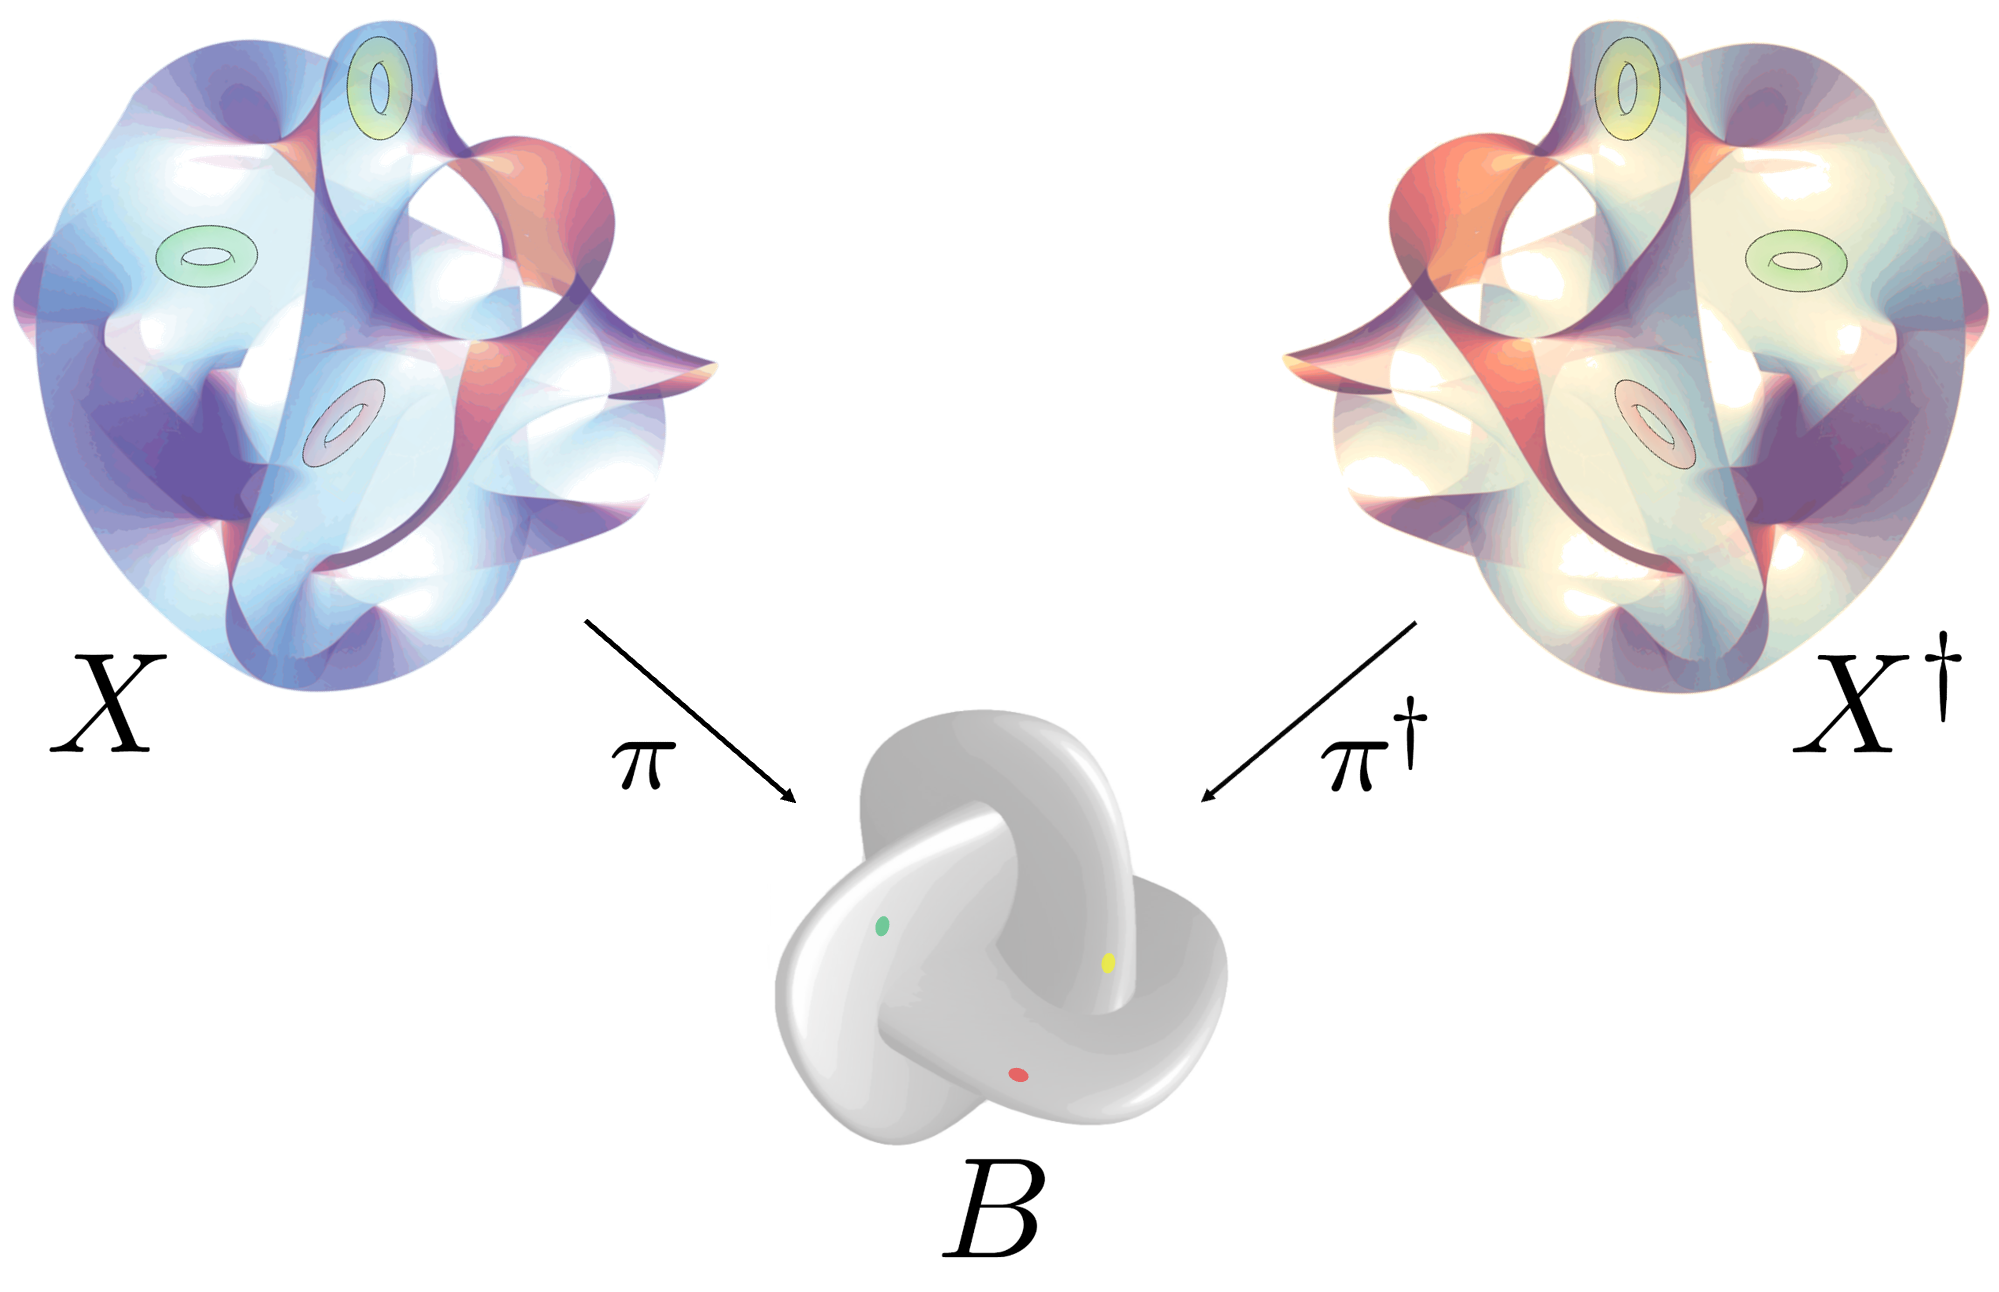
\includegraphics[width=0.62\linewidth]{fig15.png}
  \caption{SYZ 猜想把镜像 Calabi--Yau 流形对 $(X,X^\dagger)$ 的纤维（特殊拉格朗日环面）联系起来。（来源：\url{http://hci.stanford.edu/~cagatay/projects/boys/Demiralp-2009-CLF.pdf}、\url{https://plus.maths.org/content/hidden-dimensions}；特别感谢 KoMa，他建议了编辑此图及许多其他图的最佳方式。）\hfill（原书 p.127）}
  \label{fig:15}
\end{figure}

% ============================================================================
%  展望  （原书 p.128，PDF p.131）
% ============================================================================
\clearpage
\section*{展望}
\addcontentsline{toc}{section}{展望}

在结束讨论之前，作一点回顾是应当的。同调镜像对称带我们走过了一段旅程：从大量"抽象废话"
（也就是范畴论与同调代数）出发，进入 Floer 理论所刻画的几何领域，最终又拱回
Kontsevich 的代数猜想，即我们最初声明的目标。这条抛物线要求我们向纯粹数学的许多基础
分支借用概念：辛几何与复几何、泛函分析的影子、无处不在的代数拓扑，最后还有代数几何的
一瞥——而这一切始终有范畴论的记号作伴。无需多言，我们才刚刚触及这个主题所能提供之物的
皮毛。而正是在这种看似永无止境的可能性中，也许就藏着它不可否认的魅力。

毕竟，一个尝试性的物理"万有理论"会汇聚如此丰富的数学、并指出其间的意外联系，从而提升
一种更微妙地交织在一起的理论图景——并反过来提升现实本身——这种愿景看来是公平的。当然，
据作者所能作出的最佳猜测，这里所呈现的部分内容已经相当过时；而同调镜像猜想至今在其最
一般的形式下仍未获证明。但教训仍在彼处，而那首交响乐值得一听。

% [Tutor Note: 【背景】"abstract nonsense" 是范畴论的戏称，源自 Mac Lane；作者用它自嘲，
% 中译保留为"抽象废话"并在括号内点明。末句 "the symphony is one worth listening to"
% 呼应前文 "symphony"，故译为"交响乐"，不译作"交响曲"以外的比喻义。]

% [Tutor Note: 【勘误】原书 p.128 正文首句 "a little retrospection is in order" 与末段
% "part of what presented here is ... already quite obsolete" 中，原文 "what presented"
% 缺系动词（应为 "what is presented"），属英文笔误，译文按语法补足，特此说明。]


% ============================================================================
%  refs.tex —— 参考文献（保留原文英文；编号与原文一致）
% ============================================================================

\begin{thebibliography}{99}

\bibitem[ABC+09]{ABCp09} P.S. Aspinwall, T. Bridgeland, A. Craw, M.R. Douglas, M. Gross, A. Kapustin, G.W. Moore, G. Segal, B. Szendröi, P.M.H. Wilson. Dirichlet branes and mirror symmetry. Clay Mathematics Monographs, vol. 4, AMS, (2009). ISBN: 978-0-8218-3848-8. URL: http://www.claymath.org/library/monographs/cmim04.pdf.

\bibitem[Abo10]{Abo10} M. Abouzaid. A geometric criterion for generating the Fukaya category. Publications mathématiques de l’IHES, Tome 112 (2010), 191–240, (September 29, 2010.) URL: https://arxiv.org/abs/1001.4593.

\bibitem[AS09]{AS09} M. Abouzaid, I. Smith. Homological mirror symmetry for the four- torus. Duke Math. J. 152, no. 3 (2010), 373–440, (July 31, 2009). URL: https://arxiv.org/abs/0903.3065v2.

\bibitem[Aur07]{Aur07} D. Auroux. Mirror symmetry and T-duality in the complement of an anticanonical divisor, (July 10, 2007). URL: https://arxiv.org/ abs/0706.3207v2.

\bibitem[Aur09]{Aur09} D. Auroux. Mirror symmetry. Lecture notes, MIT, (Spring 2009). URL: https://math.berkeley.edu/\textasciitilde{}auroux/18.969-S09/.

\bibitem[Aur13]{Aur13} D. Auroux. A beginner’s introduction to Fukaya categories, (January 29, 2013). URL: https://arxiv.org/abs/1301.7056v1.

\bibitem[BBS07]{BBS07} K. Becker, M. Becker, J. Schwarz. String theory and M-theory: A modern introduction. Cambridge University Press, (2007). ISBN: 978- 0-521-86069-7.

\bibitem[CdGP91]{CdGP91} P. Candelas, X. de la Ossa, P. Green, L. Parkes. A pair of Calabi–Yau manifolds as an exactly soluble superconformal theory. Nuclear Physics B, Vol. 359, Issue 1, 21–74, (February 1, 1991). URL: https://webspace.science.uu.nl/\textasciitilde{}beuke106/ HypergeometricFunctions/COGP.pdf.

\bibitem[CGK02]{CGK02} K. Cieliebak, V.L. Ginzburg, E. Kerman. Symplectic homology and periodic orbits near symplectic submanifolds, (November 12, 2002). URL: https://arxiv.org/abs/math/0210468v2.

\bibitem[Flo88]{Flo88} A. Floer. Morse theory for Lagrangian intersections. J. Differential Geom. 28, no. 3, 513–547, (1988). URL: https://projecteuclid.org/journals/ journal-of-differential-geometry/volume-28/issue-3/ Morse-theory-for-Lagrangian-intersections/10.4310/jdg/ 1214442477.full.

\bibitem[FOOO07]{FOOO07} K. Fukaya, Y.-G. Oh, H. Ohta, K. Ono. Lagrangian surgery and holomorphic discs. Chapter 10, (November 17, 2007). URL: https://www.math.kyoto-u.ac.jp/\textasciitilde{}fukaya/Chapter10071117.pdf.

\bibitem[FOOO09]{FOOO09} K. Fukaya, Y.-G. Oh, H. Ohta, K. Ono. Lagrangian intersection Floer theory: anomaly and obstruction. AMS/IP Studies in Advanced Mathematics, Vol. 46, (2009). ISBN: 978-0-8218-5253-8.

\bibitem[Fuk93]{Fuk93} K. Fukaya. Morse homotopy, A∞-category, and Floer homologies. In Proceedings of GARC workshop on Geometry and Topology (H.J. Kim ed.), Seoul National University, 1–102, (1993). URL: https://www.math.kyoto-u.ac.jp/\textasciitilde{}fukaya/mfikki.pdf.

\bibitem[Fuk99]{Fuk99} K. Fukaya. Floer homology for 3-manifold with boundary I. Kyoto University, (1999). URL: https://www.math.kyoto-u.ac.jp/ \textasciitilde{}fukaya/bdrt1.pdf.

\bibitem[Fuk00]{Fuk00} K. Fukaya. Mirror symmetry of abelian varieties and multi-theta functions. J. Algebraic Geom. 11, 393–512, (2000). URL: https://www.math.kyoto-u.ac.jp/\textasciitilde{}fukaya/abelrev.pdf.

\bibitem[Fuk02a]{Fuk02a} K. Fukaya. Floer homology and mirror symmetry I. (2002) URL: https://www.math.kyoto-u.ac.jp/\textasciitilde{}fukaya/mirror1.pdf.

\bibitem[Fuk02b]{Fuk02b} K. Fukaya. Floer homology and mirror symmetry II. (2002) URL: https://projecteuclid.org/download/pdf\_1/euclid.aspm/ 1546230292.

\bibitem[Gat20]{Gat20} A. Gathmann. Algebraic geometry. Lecture notes, TU Kaiserslautern, (2019–2020). URL: https://www.mathematik.uni-kl. de/\textasciitilde{}gathmann/de/alggeom-2019.php.

\bibitem[GHJ03]{GHJ03} M. Gross, D. Huybrechts, D. Joyce. Calabi–Yau manifolds and related geometries. Lectures at a Summer School in Nordfjordeid (June 2001), Springer Universitext, (2003). ISBN: 978-3-540-44059-8.

\bibitem[GJ90]{GJ90} E. Getzler, J.D.S. Jones. A∞-algebras and the cyclic bar complex. Illinois J. Math. 34, no. 2, 256–283, (1990). URL: https://cpb-us-e1.wpmucdn.com/sites.northwestern.edu/ dist/c/2278/files/2019/08/cyclic2.pdf.

\bibitem[GM03]{GM03} S.I. Gelfand, Yu.I. Manin. Methods of homological algebra. Second edition, Springer Monographs in Mathematics, (2003). ISBN: 978-3- 642-07813-2.

\bibitem[Gre97]{Gre97} B.R. Greene. String theory on Calabi–Yau manifolds. Columbia University, New York, (February 23, 1997). URL: https://arxiv.org/ abs/hep-th/9702155v1.

\bibitem[Har77]{Har77} R. Hartshorne. Algebraic Geometry. Springer Graduate Texts in Mathematics 52, (1977). ISBN: 978-1-4757-3849-0.

\bibitem[Hat09]{Hat09} A. Hatcher. Algebraic Topology. Cambridge University Press, (2009). ISBN: 978-0-521-79540-1. URL: http://pi.math.cornell. edu/\textasciitilde{}hatcher/AT/ATpage.html.

\bibitem[HKK+03]{HKKp03} K. Hori, S. Katz, A. Klemm, R. Pandharipande, R. Thomas, C. Vafa, R. Vakil, E. Zaslow. Mirror symmetry. Clay Mathematics Monographs, vol. 1, AMS, (2003). ISBN: 978-0-8218-2955- 4. URL: https://web.archive.org/web/20060919020706/http://math.stanford.edu/\textasciitilde{}vakil/files/mirrorfinal.pdf.

\bibitem[Kad80]{Kad80} T.V. Kadeishvili. On the theory of homology of fiber spaces. (Rus- sian) International Topology Conference (Moscow State Univ., Moscow, 1979). Uspekhi Mat. Nauk 35 (1980), no. 3(213), 183–188. URL: https://arxiv.org/pdf/math/0504437.pdf.

\bibitem[Kel01]{Kel01} B. Keller. Introduction to A-infinity algebras and modules. Homology Homotopy Appl. 3, (January 12, 2001). URL: https://arxiv.org/ abs/math/9910179v2.

\bibitem[Kel06]{Kel06} B. Keller. A-infinity algebras, modules and functor cate- gories. (February 12, 2006) URL: https://arxiv.org/abs/math/0510508v3.

\bibitem[Kon94]{Kon94} M. Kontsevich. Homological algebra of mirror symmetry. In Proceedings of the International Congress of Mathematicians, Birkhäuser, 120–139, (November 30, 1994). URL: https://arxiv.org/abs/ alg-geom/9411018v1.

\bibitem[KS01]{KS01} M. Kontsevich, Y. Soibelman. Homological mirror symmetry and torus fibrations. (June 4, 2001). URL: https://arxiv.org/abs/ math/0011041v2.

\bibitem[Lef03]{Lef03} K. Lefèvre-Hasegawa. Sur les A∞-catégories. PhD thesis, Université Paris 7, (October 21, 2003). URL: https://arxiv.org/abs/math/ 0310337v1.

\bibitem[LP11]{LP11} Y. Lekili, T. Perutz. Fukaya categories of the torus and Dehn surgery. (March 4, 2011) URL: https://arxiv.org/abs/1102.3160.

\bibitem[May01]{May01} J.P. May. The axioms for triangulated categories, edited extract from The additivity of traces in triangulated categories, Advances in Math- ematics 163, 34—73, (2001). URL: http://www.math.uchicago.edu/\textasciitilde{}may/MISC/Triangulate.pdf.

\bibitem[McS94]{McS94} D. McDuff, D. Salamon. J-holomorphic curves and quantum co- homology. University Lecture Series, Vol. 6, AMS, (1994). ISBN: 0-8218-0332-8. URL: https://people.math.ethz.ch/\textasciitilde{}salamon/ PREPRINTS/jholsm.pdf (May 1995).

\bibitem[Mer14]{Mer14} W.J. Merry. Floer theory. Lecture notes, ETH Zürich, (2013–2014). URL: https://www.merry.io/other-notes/floer-theory/.

\bibitem[Mer18]{Mer18} W.J. Merry. Algebraic topology. Lecture notes, ETH Zürich, (2017–2018). URL: https://www.merry.io/courses/ algebraic-topology/.

\bibitem[Mer19]{Mer19} W.J. Merry. Differential geometry. Lecture notes, ETH Zürich, (2018–2019). URL: https://www.merry.io/courses/ differential-geometry/.

\bibitem[Moo05]{Moo05} G. Moore. What is... a brane?. Notices of the AMS, vol. 52, no. 2, 214–215, (February 2005). URL: http://www.ams.org/notices/ 200502/what-is.pdf.

\bibitem[MS74]{MS74} J.W. Milnor, J.D. Stasheff. Characteristic classes. Annals of Math- ematics Studies, no. 76, Princeton University Press; University of Tokyo Press, (1974). ISBN: 978-0-691-08122-9. URL: https://www. maths.ed.ac.uk/\textasciitilde{}v1ranick/papers/milnstas.pdf.

\bibitem[Oh91]{Oh91} Y.-G. Oh. Symplectic topology and Floer homology. IBS Center for Geometry and Physics, and Pohang University of Science and Tech- nology, Republic of Korea. Cambridge University Press, (1991). URL: https://cgp.ibs.re.kr/\textasciitilde{}yongoh/all.pdf.

\bibitem[PZ00]{PZ00} A. Polishchuk, E. Zaslow. Categorical mirror symmetry: the elliptic curve. Adv. Theor. Math. Phys. 4, 1187–1207, (April 7, 2000). URL: https://arxiv.org/abs/math/9801119v3.

\bibitem[Sal97]{Sal97} D. Salamon. Lectures on Floer homology. IAS/Park City Gradu- ate Summer School on Symplectic Geometry and Topology, (De- cember 1, 1997). URL: https://people.math.ethz.ch/\textasciitilde{}salamon/ PREPRINTS/floer.pdf.

\bibitem[Sei99]{Sei99} P. Seidel. Lagrangian two-spheres can be symplectically knotted. J. Differential Geom. 52, 145–171, (May 31, 2000). URL: https://arxiv.org/abs/math/9803083.

\bibitem[Sei02]{Sei02} P. Seidel. A long exact sequence for symplectic Floer cohomology. Revised version, Topology 42, 1003–1063, (July 20, 2002). URL: https://arxiv.org/abs/math/0105186v2.

\bibitem[Sei08]{Sei08} P. Seidel. Fukaya categories and Picard-Lefschetz theory. Zurich Lec- tures in Advanced Mathematics, European Mathematical Society, (2008). ISBN: 978-3-03719-063-0.

\bibitem[Sei11]{Sei11} P. Seidel. Homological mirror symmetry for the genus two curve. (August 21, 2011) URL: https://arxiv.org/abs/0812.1171v5.

\bibitem[Sei13]{Sei13} P. Seidel. Homological mirror symmetry for the quartic surface. (August 6, 2013) URL: https://arxiv.org/abs/math/0310414v4.

\bibitem[Sil12]{Sil12} A.C. da Silva. Lectures on symplectic geometry. Lecture Notes in Mathematics, Springer, (2008). ISBN: 978-3-540-45330-7. URL: https://people.math.ethz.ch/\textasciitilde{}acannas/Papers/lsg.pdf (January 2006).

\bibitem[Sta63]{Sta63} J.D. Stasheff. Homotopy associativity of H-spaces, I-II. Trans. of AMS, Vol. 108, 275–292 resp. 293–312, (August 1963). URL: https://www.ams.org/journals/tran/1963-108-02/ S0002-9947-1963-99936-3/S0002-9947-1963-99936-3.pdf resp. https://www.ams.org/journals/tran/1963-108-02/ S0002-9947-1963-0158400-5/S0002-9947-1963-0158400-5. pdf.

\bibitem[SYZ96]{SYZ96} A. Strominger, S.-T. Yau, E. Zaslow. Mirror symmetry is T-duality. Nucl. Phys. B479, 243–259, (June 14, 1996). URL: https://arxiv. org/abs/hep-th/9606040v2.

\bibitem[Ver96]{Ver96} J.-L. Verdier. Des catégories dérivées des catégories abéliennes. Astérisque 239, Société Mathématique de France, (1996). URL: http://www.numdam.org/issue/AST\_1996\_\_239\_\_R1\_0.pdf.

\bibitem[Wen14]{Wen14} C. Wendl. Lectures on holomorphic curves in symplectic and contact geometry. University College London, (May 27, 2014). URL: https://arxiv.org/abs/1011.1690v2.

\bibitem[YN10]{YN10} S.-T. Yau, S. Nadis. The shape of inner space: string theory and the geometry of the universe’s hidden dimensions. Basic Books, (2010). ISBN: 978-0-465-02023-2.

\bibitem[Zwi09]{Zwi09} B. Zwiebach. A first course in string theory. Cambridge University Press, (2009). ISBN: 978-0-521-88032-9.

\end{thebibliography}
% ============================================================================
%  appendix_glossary.tex —— 英中术语对照表（译者增补，非原文内容）
%  由 work/GLOSSARY.md 生成；修改词表后重跑 tools/mkglossary.py
% ============================================================================

\appendix
\section{英中术语对照表}
\label{app:glossary}

本表由译者补入，原文并无此附录。所列为全书反复出现的核心术语，按主题分组；
数学专名（Kontsevich、Fukaya、Calabi--Yau、Floer 等）与记号一律保留原文，不作音译。

\vspace{0.6em}
\noindent\textbf{A∞ 与同调代数}\par\nobreak
\vspace{0.3em}
{\small
\begin{longtable}{p{0.42\textwidth}p{0.42\textwidth}}
\toprule
English & 中文 \\
\midrule
\endhead
$A_\infty$-algebra / category / functor / module & $A_\infty$-代数 / 范畴 / 函子 / 模 \\
$A_\infty$-space & $A_\infty$-空间 \\
non-unital / strictly unital / cohomologically unital (c-unital) & 非幺的 / 严格幺的 / 上同调幺的（c-幺的） \\
unitality & 幺性 \\
unit & 单位元 \\
associahedron ($K_n$) & 结合面体（$K_n$，保留记号） \\
pre-natural transformation & 预自然变换 \\
natural transformation & 自然变换 \\
cohomological category & 上同调范畴 \\
quasi-equivalence & 拟等价 \\
quasi-isomorphism & 拟同构 \\
homotopy equivalence & 同伦等价 \\
homotopic & 同伦的 \\
homotopy unit & 同伦单位元 \\
Homological Perturbation Lemma & 同调微扰引理 \\
Hochschild cohomology & Hochschild 上同调 \\
Koszul sign rule & Koszul 符号法则 \\
suspension $SV=V[1]$ / shift $[n]$ & 悬挂 $SV=V[1]$ / 平移 $[n]$ \\
graded vector space / degree & 分次向量空间 / 次数 \\
differential & 微分 \\
cochain complex / cochain map & 上链复形 / 上链映射 \\
Yoneda embedding & Yoneda 嵌入 \\
representable functor & 可表函子 \\
enriched category & 富化范畴 \\
mapping cone / cone & 映射锥 / 锥 \\
exact triangle & 正合三角形 \\
distinguished triangle & 区分三角形（distinguished triangle） \\
triangulated / pre-triangulated & 三角的 / 预三角的 \\
translation functor & 平移函子 \\
octahedral axiom / Verdier's axiom & 八面体公理 / Verdier 公理 \\
twisted complex & 扭复形 \\
twisting & 扭转 \\
convolution & 卷积 \\
split-closed / split-closure & 分裂封闭的 / 分裂封闭 \\
split-generation / split-generate & 分裂生成 \\
idempotent & 幂等 \\
direct summand & 直和项 \\
abstract image & 抽象像 \\
bounded derived category $\mathsf{D}^{\mathrm b}$ & 有界导出范畴 \\
split-closed derived category $\mathsf{D}^\pi$ & 分裂封闭导出范畴 \\
formal / formality & 形式的 / 形式性 \\
minimal model & 极小模型 \\
spectral sequence & 谱序列 \\
exact sequence & 正合列 \\
cokernel / kernel & 余核 / 核 \\
additive / abelian category & 加性范畴 / 阿贝尔范畴 \\
object / morphism / functor & 对象 / 态射 / 函子 \\
hom-set & Hom 集 \\
full / faithful & 全的 / 忠实的 \\
\bottomrule
\end{longtable}}

\vspace{0.6em}
\noindent\textbf{辛几何与 Floer 理论}\par\nobreak
\vspace{0.3em}
{\small
\begin{longtable}{p{0.42\textwidth}p{0.42\textwidth}}
\toprule
English & 中文 \\
\midrule
\endhead
symplectic manifold / form & 辛流形 / 辛形式 \\
almost complex structure / compatible & 近复结构 / 相容的 \\
$J$-holomorphic & $J$-全纯 \\
Lagrangian submanifold & 拉格朗日子流形 \\
exact / monotone Lagrangian & 正合 / 单调拉格朗日（子流形） \\
special Lagrangian & 特殊拉格朗日 \\
Floer complex / differential / cohomology & Floer 复形 / 微分 / 上同调 \\
Lagrangian Floer cohomology & 拉格朗日 Floer 上同调 \\
Maslov index / class & Maslov 指标 / 类 \\
grading / graded & 分次 / 分次的 \\
transversality / regular & 横截性 / 正则的 \\
moduli space & 模空间 \\
compactness / bubbling / strip breaking / disk bubbling & 紧致性 / 冒泡 / 条带断裂 / 圆盘冒泡 \\
gluing & 粘接 \\
punctured disk / boundary puncture & 穿孔圆盘 / 边界穿孔 \\
strip & 条带 \\
energy & 能量 \\
Novikov ring / field & Novikov 环 / 域 \\
completion & 完备化 \\
Fukaya category & Fukaya 范畴 \\
wrapped Fukaya category & wrapped Fukaya 范畴（wrapped 不译） \\
stop & stop（不译） \\
Liouville manifold / form / vector field & Liouville 流形 / 形式 / 向量场 \\
Lagrangian handle / connected sum & 拉格朗日把手 / 连通和 \\
Dehn twist & Dehn 扭转 \\
vanishing cycle / thimble & 消没圈 / thimble（顶针，首次括注） \\
Lefschetz fibration & Lefschetz 纤维化 \\
cotangent bundle / unit cotangent bundle & 余切丛 / 单位余切丛 \\
symplectomorphism & 辛同胚 \\
Hamiltonian / Hamiltonian vector field & 哈密顿（量）/ 哈密顿向量场 \\
moment map & 矩映射 \\
action functional & 作用量泛函 \\
contractible & 可缩的 \\
\bottomrule
\end{longtable}}

\vspace{0.6em}
\noindent\textbf{镜像对称}\par\nobreak
\vspace{0.3em}
{\small
\begin{longtable}{p{0.42\textwidth}p{0.42\textwidth}}
\toprule
English & 中文 \\
\midrule
\endhead
mirror symmetry / mirror pair & 镜像对称 / 镜像对 \\
Homological Mirror Symmetry (HMS) & 同调镜像对称（HMS） \\
A-side / B-side & A-侧 / B-侧 \\
A-model / B-model & A-模型 / B-模型 \\
D-brane / open string / closed string & D-膜 / 开弦 / 闭弦 \\
worldsheet & 世界面 \\
Calabi–Yau manifold & Calabi–Yau 流形 \\
Kähler manifold / Kähler class & Kähler 流形 / Kähler 类 \\
complexified Kähler class & 复化 Kähler 类 \\
Hodge diamond / Hodge number & Hodge 菱形 / Hodge 数 \\
coherent sheaf & 凝聚层 \\
bounded derived category of coherent sheaves & 凝聚层的有界导出范畴 \\
Fourier–Mukai transform & Fourier–Mukai 变换 \\
T-duality & T-对偶 \\
SYZ conjecture / torus fibration & SYZ 猜想 / 环面纤维化 \\
quantum cohomology & 量子上同调 \\
Gromov–Witten invariant & Gromov–Witten 不变量 \\
Yukawa coupling & Yukawa 耦合 \\
elliptic curve / genus & 椭圆曲线 / 亏格 \\
deformation / moduli & 形变 / 模 \\
large complex structure limit & 大复结构极限 \\
hyperkähler & 超 Kähler \\
mirror map & 镜像映射 \\
\bottomrule
\end{longtable}}

\vspace{0.6em}
\noindent\textbf{结构词}\par\nobreak
\vspace{0.3em}
{\small
\begin{longtable}{p{0.42\textwidth}p{0.42\textwidth}}
\toprule
English & 中文 \\
\midrule
\endhead
Introduction / Outlook / References / Index & 引言 / 展望 / 参考文献 / 索引 \\
Part / Chapter / Section / Subsection & 部分 / 章 / 节 / 小节 \\
Theorem / Lemma / Proposition / Corollary / Conjecture & 定理 / 引理 / 命题 / 推论 / 猜想 \\
Definition / Example / Remark / Proof & 定义 / 例 / 注 / 证明 \\
Definition (as heading inside text) & 定义 \\
"It is obvious that …" & "显然……"（批注中说明省略了什么） \\
up to isomorphism & 在同构意义下 \\
without loss of generality & 不失一般性 \\
the reader may check & 读者可自行验证 \\
\bottomrule
\end{longtable}}


\end{document}
